\documentclass[11pt]{report}

\usepackage{epsf,epsfig,subfigure,latexsym,makeidx,latexsym,xspace,amssymb}

\pagestyle{headings}

% LaTeX Size Stuff
%-----------------
\newcommand{\newsched}{Batched Scheduling}
\newcommand{\Newsched}{Batched Scheduling}
\newcommand{\NewSched}{Batched Scheduling}
\newcommand{\Oldsched}{Single Stack Scheduling}
\newcommand{\OldSched}{Single Stack Scheduling}
\newcommand{\oldsched}{Single Stack Scheduling}
\newcommand{\localsched}{Local Scheduling}
\newcommand{\Localsched}{Local Scheduling}
\newcommand{\LocalSched}{Local Scheduling}

\setlength{\topmargin}{-0.25in}
\setlength{\headheight}{10pt}
\setlength{\headsep}{30pt}
\setlength{\oddsidemargin}{0.0in}
\setlength{\evensidemargin}{0.0in}
\setlength{\textheight}{8.5in}
\setlength{\textwidth}{6.5in}
\setlength{\footskip}{50pt}
\setlength{\parskip}{2mm}               % space between paragraphs

\def\cut{\mbox{\tt '!'/0}}
\def\not{\mbox{${\tt '\backslash+'/1}$}}

\newtheorem{example}{Example}[section]

\newenvironment{Prog}{\begin{tt}\begin{tabular}[c]{l}}{\end{tabular}\end{tt}}

\newcommand{\comment}[1]{}
\newcommand{\ourprolog}{XSB}
\newcommand{\smallourprolog}{xsb}
\newcommand{\version}{Version 2.2}
\newcommand{\LRD}{LRD-stratified}

\newcommand{\demo}[1]{\hspace*{1.5cm}{\tt #1}}
\newcommand{\desc}[1]{\item[{\tt #1}]\hspace*{1mm}\newline}
\newcommand{\desce}[1]{\item[{\tt #1}]}
\newcommand{\ourrepeatitem}[1]{\item[{\mbox{\tt #1}}]\ \\ \vspace*{-.35in}}
\newcommand{\ouritem}[1]{\item[{\mbox{\tt #1}}]\ \\}
\newcommand{\ournewitem}[2]{\item[{\mbox{\tt #1}}]\hspace*{\fill}{\mbox{\sf #2}}\ \\}

\newcommand{\stuff}[1]{
        \begin{minipage}{4in}
        {\tt \samepage
        \begin{tabbing}
        \hspace{8mm} \= \hspace{6mm} \= \hspace{10mm} \= \hspace{55mm} \= \kill
        #1 \hfill
        \end{tabbing}
        }
        \end{minipage}
}

\newcommand{\longline}{\noindent\rule{\textwidth}{.01in}}

%------------------------------------------------------------
\input{predindex.sty}
\makepredindex
\makeindex
%------------------------------------------------------------

\begin{document}

\title{\bf The XSB System \\ \version \\ Volume 1: Programmer's Manual}

\author{{\epsfxsize=230pt \epsfbox{xsb-logo.eps}}\\
        \ \\ \ \\
        {\em Konstantinos Sagonas} \\
        {\em Terrance Swift} \\
        {\em David S. Warren} \\ 
        {\em Juliana Freire} \\
        {\em Prasad Rao} \\
        \ \\ \\ \\
        {\normalsize with contributions from} \\
        {\em Steve Dawson} \\
        {\em Michael Kifer} \\
        \ \\
} 

%%\date{November 1999}

\maketitle

\thispagestyle{empty}
\begin{center}
{\bf {\Large 
		Credits
            %=============%
}}
\end{center}

% Apologies to anyone I left out...  It wasn't intentional! TLS.

\begin{quote}
Day-to-day care and feeding of XSB including bug fixes, ports, and
configuration management has been done by Kostis Sagonas, David
Warren, Terrance Swift, Prasad Rao, Steve Dawson, Juliana Freire,
Ernie Johnson, Baoqiu Cui, Michael Kifer, Bart Demoen and Luis F.
Castro.

In \version, the core engine development of the SLG-WAM has been
mainly implemented by Terrance Swift, Kostis Sagonas, Prasad Rao,
Juliana Freire, Ernie Johnson, Luis Castro and Rui Marques.  The
breakdown, very roughly, was that Terrance Swift wrote the initial
tabling engine, the SLG-WAM, and builtins.  Prasad Rao reimplemented
the engine's tabling subsystem to use tries for variant-based table
access and Ernie Johnson extended and refactored these routines in a
number of ways, including adding call subsumption.  Kostis Sagonas
implemented most of tabled negation.  Juliana Freire revised the table
scheduling mechanism starting from Version~1.5.0 to create the batched
and local scheduling that is currently used.  Baoqiu Cui revised the
data structures used to maintain delay lists, and added attributed
variables to the engine.  Finally, Luis Castro rewrote the emulator to
use jump tables and wrote a heap-garbage collector for the SLG-WAM.
Rui Marques was mainly responsible for making XSB multi-threaded, as
well as for the concurrency control algorithms used for shared tables.

Other engine work includes the following.  Memory expansion code for
WAM stacks was written by Ernie Johnson and Bart Demoen.  Heap garbage
collection was written by Luis de Castro, Kostis Sagonis and Bart
Demoen.  Rui Marques improved the trailing of the SLG-WAM and rewrote
much of the engine to make it compliant with 64-bit architectures.
Assert and retract code was based on code written by Jiyang Xu and
significantly revised by David S. Warren, who added alternative,
multiple, and star indexing.  Trie assert/retract code, and trie
interning code was written by Prasad Rao, as was most code for
reclaiming table space. The current version of {\tt findall/3} was
re-written from scratch by Bart Demoen, as was XSB's throw and catch
mechanism.  64-bit floats were added by Charles Rojo.

In terms of Prolog code, Kostis Sagonas was responsible for HiLog
compilation and associated builtins.  Steve Dawson implemented
Unification Factoring.  The revision of XSB's I/O into ISO-compatable
streams was done by Michael Kifer and Terrance Swift.  The {\tt
  auto\_table} and {\tt suppl\_table} directives were written by
Kostis Sagonas.  The DCG expansion module was written by Kostis
Sagonas for non-tabled code and by Baoqiu Cui, Terrance Swift and
David Warren for tabled code.  The handling of the {\tt multifile}
directive was written by Baoqiu Cui. C.R. Ramakrishnan wrote the mode
analyzer for XSB.  Michael Kifer implemented the {\tt storage} module.

For configuration management, Michael Kifer rewrote parts of the XSB
code to make XSB configurable with GNU's Autoconf, implemented XSB's
package system, and integrated GPP with XSB's compiler.  GPP, the
source code preprocessor used by XSB, was written by Denis Auroux, who
also wrote the GPP manual reproduced in Appendix A.

The starting point of XSB (in 1990) was PSB-Prolog 2.0 by Jiyang Xu.
PSB-Prolog in its turn was based on SB-Prolog, primarily designed and
written by Saumya Debray, David S. Warren, and Jiyang Xu.  Thanks are
also due to Weidong Chen for his work on Prolog clause indexing for
SB-Prolog, to Richard O'Keefe, who contributed the Prolog code for the
Prolog reader and the C code for the tokenizer, and to Ciao Prolog
whose {\tt write\_term/[2,3]} we use.

... Now what did I forget this time ?

\end{quote}

%%% Local Variables: 
%%% mode: latex
%%% TeX-master: "manual1"
%%% End: 

\newpage
\thispagestyle{empty}
%\input{Acknowl}
%\newpage

\pagenumbering{roman}
\tableofcontents
\newpage        % Just to avoid a silly LaTeX bug with \pagenumbering
  
\pagenumbering{arabic}

\chapter{Introduction} \label{introduction}
%==========================================

XSB is a research-oriented, commercial-grade Logic Programming system
for Unix and Windows-based platforms.  In addition to providing nearly
all functionality of ISO-Prolog, XSB includes the following features:
\begin{itemize}
%
\item Evaluation of queries according to the Well-Founded Semantics
  \cite{VGRS91} through full SLG resolution;
%
\item A fully multi-threaded evaluation mechanism with thread-shared
  static code, and that allows dynamic code and tables to be
  thread-shared or thread-private.
%
\item Constraint handling for tabled programs based on an engine-level
  implementation of annotated variables and a package, {\tt clpqr} for
  handling real constraints, and the addition of Constraint Handling
  Rules \cite{};
% 
\item A variety of indexing techniques for asserted code 
  including variable-depth indexing on several alternate arguments,
  fixed-depth indexing on combined arguments, trie-indexing.  In
  addition, both backtrackable and non-backtrackable updates to asserted
  code are supported.
%
\item A set of mature packages, to extend XSB to evaluate
  F-logic~\cite{KLW95} through the {\em FLORA} package, to model check
  concurrent systems through the {\em XMC} system, to manage
  ontologies through the {\em Cold Dead Fish} package, to support
  literate programming through the {\tt xsbdoc} package, and to
  support answer set programming through the {\tt XASP} package among
  other features.
%
\item A number of interfaces to other software systems, such a C, Java,
  Perl, ODBC, SModels \cite{NiSi97}, and Oracle.
%
\item Fast loading of large files by the {\tt load\_dync}
  predicate, and by other means.
%
\item A compiled HiLog implementation;
%
\item Backtrackable updates through XSB's {\tt storage} module that
  support the semantics of transaction logic \cite{BoKi94}.
%
\item Extensive pattern matching packages, and interfaces to libwww
  routines, all of which are especially useful for Web applications.
%
\item A novel transformation technique called {\em unification
factoring} that can improve program speed and indexing for compiled
code; 
%
\item Macro substitution for Prolog files via the {\tt xpp}
  preprocessor (included with the XSB distribution).
%
\item Preprocessors and Interpreters so that XSB can be used to evaluate
  programs that are based on advanced formalisms, such as extended logic
  programs (according to the Well-Founded Semantics \cite{ADP94});
  Generalized Annotated Programs \cite{KiSu92}.
%
\item Source code availability for portability and extensibility under
  the GNU General Public Library License.
\end{itemize}
 
Though XSB can be used as a Prolog system\footnote{Many of the Prolog
  components of XSB were originally based on PSB-Prolog~\cite{Xu90},
  which itself is based on version 2.0 of SB-Prolog~\cite{Debr88}.},
we avoid referring to XSB as such, because of the availability of SLG
resolution and the handling of HiLog terms.  These facilities, while
seemingly simple, significantly extend its capabilities beyond those
of a typical Prolog system. We feel that these capabilities justify
viewing XSB as a new paradigm for Logic Programming.  We briefly
discuss some of these features; others are discussed in Volumes 1 and
2 of the XSB manual, as well as the manuals for various XSB packages
such as FLORA, XMC, Cold Dead Fish, xsbdoc, and XASP.

\paragraph{Well-Founded Semantics} To understand the implications of
SLG resolution \cite{ChWa96}, recall that Prolog is based on a
depth-first search through trees that are built using program clause
resolution (SLD).  As such, Prolog is susceptible to getting lost in
an infinite branch of a search tree, where it may loop infinitely.
SLG evaluation, available in XSB, can correctly evaluate many such
logic programs.  To take the simplest of examples, any query to the
program:
\begin{center}
\begin{minipage}{3.8in}
\begin{verbatim}
:- table ancestor/2.

ancestor(X,Y) :- ancestor(X,Z), parent(Z,Y).
ancestor(X,Y) :- parent(X,Y).
\end{verbatim}
\end{minipage}
\end{center}
will terminate in XSB, since {\tt ancestor/2} is compiled as a tabled
predicate; Prolog systems, however, would go into an infinite loop.
The user can declare that SLG resolution is to be used for a predicate
by using {\tt table} declarations, as here.  Alternately, an {\tt
auto\_table} compiler directive can be used to direct the system to
invoke a simple static analysis to decide what predicates to table
(see Section~\ref{tabling_directives}).  This power to solve recursive
queries has proven very useful in a number of areas, including
deductive databases, language processing \cite{syntactica, semantica},
program analysis \cite{DRW96, CoDS96, Boul97}, model checking
\cite{RRRSSW97} and diagnosis \cite{GSTPD00}.  For efficiency, we
have implemented SLG at the abstract machine level so that tabled
predicates will be executed with the speed of compiled Prolog.  We
finally note that for definite programs SLG resolution is similar to
other tabling methods such as OLDT resolution~\cite{TaSa86} (see
Chapter
\ref{chap:TablingOverview} for details).

\begin{example} \label{ex:Russell}
The use of tabling also makes possible the evaluation of programs with
non-stratified negation through its implementation of the {\em
well-founded semantics} \cite{VGRS91}.  When logic programming rules
have negation, paradoxes become possible.  As an example consider one
of Russell's paradoxes --- 
the barber in a town shaves every person who does not shave himself ---
written as a logic program.
\begin{center}
\begin{verbatim} 
:- table shaves/2.

shaves(barber,Person):- person(Person), tnot(shaves(Person,Person)).
person(barber).
person(mayor).
\end{verbatim} 
\end{center}
Logically speaking, the meaning of this program should be that the
barber shaves 
the mayor, but the case of the barber is trickier.  If we conclude
that the barber does not shave himself our meaning does not reflect the 
first rule in the program.  If we conclude that the barber does shave
himself, we have reached that conclusion using information beyond what 
is provided in the program.  The well-founded semantics, does not
treat{\tt shaves(barber,barber)} as either true or false, but as {\em
undefined}. 
Prolog, of course, would enter an infinite loop.  XSB's treatment of
negation is discussed further in Chapter \ref{chap:TablingOverview}.
\end{example}

\index{multi-threading}
\paragraph{Multi-threading} New to \version{} of XSB is a thorough
revision of XSB to support multi-threading using Posix or
Windows-level threads.  Detached XSB threads can be created to execute
specific tasks, and these threads will exit when the query succeeds
(or fails) and all thread memory reclaimed.  While a thread's
execution state is, of course, private, it shares many resources with
other threads, such as static code and I/O streams.  Dynamic code and
tables are thread-private by default, but if a predicate is declared
thread-shared, any dynamic code and tables for this predicate will be
shared among threads.  {\sc should mention something about, shared
  completed tables}.

We also note that tabled programs can be used with attributed
variables, leading to constraint tabled programs (see Volume 2 of this
manual for a discussion of the interfaces to attributed variables).

\comment{TLS: constraint handling?}

\index{indexing!star-indexing}
\paragraph{Indexing Methods} Data oriented applications may also
require indices other than Prolog's first argument indexing.  XSB
offers a variety of indexing techniques for asserted code.  Clauses
can be indexed on a group of arguments or on alternative arguments.
For instance, the executable directive {\tt index(p/4,[3,2+1])}
specifies indexes on the (outer functor symbol of) the third argument
{\em or} on a combination of (the outer function symbol of) the second
and first arguments.  If data is expected to be structured within
function symbols and is in unit clauses, the directive {\tt
  index(p/4,trie)} constructs an indexing trie of the {\tt p/4}
clauses using a depth-first, left-to-right traversal through each
clause.  Representing data in this way allows discrimination of
information nested arbitrarily deep within clauses.  Advantages of
both kinds of indexing can be combined via {\em star-indexing}.
Star-indexing indicates that up to the first 5 fields in an argument
will be used for indexing (the ordering of the fields is via a
depth-first traversal).  For instance, {\tt index(p/4,[*(4),3,2+1])}
acts as above, but looks within 4th argument of {\tt p/4} before
examining the outer functor of argument 3 (and finally examining the
outer functors of arguments 2 and 1 together.  Using such indexing XSB
routinely performs efficiently perform intensive analyses of in-memory
knowledge bases with millions of highly structured facts.  Indexing
techniques for asserted code are covered in Section \ref{sec:assert}.

\index{InterProlog} \index{ODBC Interface}
\paragraph{Interfaces} A number of interfaces are available to link XSB
to other systems.  In UNIX systems XSB can be directly linked into C
programs; in Windows-based system XSB can be linked into C programs
through a DLL interface.  On either class of operating system, C
functions can be made callable from XSB either directly within a
process, or using a socket library.  XSB can also inter-communicate
with Java through the InterProlog interface, \footnote{InterProlog is
  available at \url{www.declarativa.com/InterProlog/default.htm}.}, or
YJXSB.  Within Interprolog, XSB and Java can be linked either through
Java's jni interface, or through sockets.  XSB can access external
data in a variety of ways: through an ODBC interface, through an
Oracle interface, or through a variety of mechanisms to read data from
flat files.  These interfaces are all described in Volume 2 of this
manual.

\paragraph{Fast Loading of Code}  A further goal of XSB is to provide
in implementation engine for both logic programming and for
data-oriented applications such as in-memory deductive database
queries and data mining \cite{SaSw94}.  One prerequisite for this
functionality is the ability to load a large amount of data very
quickly.  We have taken care to code in C a compiler for asserted
clauses.  The result is that the speed of asserting and retracting
code is faster in XSB than in any other Prolog system of which we are
aware, even when some of the sophisticated indexing mechanisms
described above are employed.  At the same time, because asserted code
is compiled into SLG-WAM code, the speed of executing asserted code in
XSB is faster than that of many other Prologs as well.  We note
however, that XSB does not follow the ISO-semantics of
assert~\cite{LiOk87}.

\paragraph{HiLog} XSB also supports HiLog programming
\cite{ChKW93,SaWa95}.  HiLog allows a form of higher-order
programming, in which predicate ``symbols'' can be variable or
structured.  For example, definition and execution of {\em generic
  predicates} like this generic transitive closure relation are
allowed:
\begin{center}
\begin{minipage}{3.7in}
\begin{verbatim}
closure(R)(X,Y) :- R(X,Y).
closure(R)(X,Y) :- R(X,Z), closure(R)(Z,Y).
\end{verbatim}
\end{minipage}
\end{center}
where {\tt closure(R)/2} is (syntactically) a second-order predicate
which, given any relation {\tt R}, returns its transitive closure
relation {\tt closure(R)}.  With XSB, support is provided for reading and
writing HiLog terms, converting them to or from internal format as
necessary (see Section~\ref{HiLog2Prolog}).  Special meta-logical
standard predicates (see Section~\ref{MetaLogical}) are also provided
for inspection and handling of HiLog terms.  Unlike earlier versions
of XSB (prior to version 1.3.1) the current version automatically
provides {\em full compilation of HiLog predicates}.  As a result,
most uses of HiLog execute at essentially the speed of compiled
Prolog.  For more information about the compilation scheme for HiLog
employed in XSB see~\cite{SaWa95}.

HiLog can also be used with tabling, so that the program above can also be
written as:
\begin{center}
\begin{minipage}{3.7in}
\begin{verbatim}
:- hilog closure.
:- table apply/3.

closure(R)(X,Y) :- R(X,Y).
closure(R)(X,Y) :- closure(R)(X,Z), R(Z,Y).
\end{verbatim}
\end{minipage}
\end{center}
as long as the underlying relations (the predicate symbols to which
$R$ will be unified) are also declared as Hilog.  For example, if {\tt
a/2} were a binary relation to which the {\tt closure} predicate would
be applied, then the declaration {\tt :- hilog a.} would also need to
be included.

\paragraph{Unification Factoring} For compiled code, XSB offers {\em
  unification factoring}, which extends clause indexing methods found
in functional programming into the logic programming framework.
Briefly, unification factoring can offer not only complete indexing
through non-deterministic indexing automata, but can also $factor$
elementary unification operations.  The general technique is described
in \cite{DRSS96}, and the XSB directives needed to use it are covered
in Section \ref{the_compiler}.

\index{Flora} \index{xsbdoc} \index{XASP}
\paragraph{XSB Packages} Based on these features, a number of
sophisticated packages have been implemented using XSB.  For instance,
XSB supports a sophisticated object-oriented interface called {\em
  Flora}.  {\em Flora} (\url{http://flora.sourceforge.net}) is
available as an XSB package and is described in its own manual,
available from the same site from which XSB was downloaded.  Another
package, XMC \url{http://www.cs.sunnysb.edu/~lmc} depends on XSB to
perform sophisticated model-checking of concurrent systems.  Within
the XSB project, the Cold Dead Fish package supports maintenance of,
and reasoning over ontologies; xsbdoc supports literate programming in
XSB, and XASP provides an interface to Smodels to support Answer Set
programming.  XSB packages also support Perl-style pattern matching
and Posix-style pattern matching.  In addition, experimental
preprocessing libararies currently supported are Extended logic
programs (under the well-founded semantics), and Annotated Logic
Programs.  These latter libraries are described in Volume 2 of this
manual.

\section{Using This Manual}
It should be mentioned that we adopt some standard notational
conventions, such as the name/arity convention for describing
predicates and functors, {\tt +} to denote input arguments, {\tt -} to
denote output arguments, {\tt ?} for arguments that may be either
input or output and {\tt \#} for arguments that are both input and
output (can be changed by the procedure).  See Section
\ref{mode_declarations} for more details.
\index{notational conventions}  Also, the manual uses UNIX syntax for
files and directories except when it specifically addresses other
operating systems such as Windows.  

Finally, we note that XSB is under continuous development, and this
document ---intended to be the user manual--- reflects the current
status (\version) of our system.  While we have taken great effort to
create a robust and efficient system, we would like to emphasize that
XSB is also a research system and is to some degree experimental.
When the research features of XSB --- tabling, HiLog, and Indexing
Techniques --- are discussed in this manual, we also cite documents
where they are fully explained.  All of these documents can be found
via the world-wide web or anonymous ftp from {\tt
$\{$www/ftp$\}$.cs.sunysb.edu}, the same host from which XSB can be
obtained.

While some of \version\ is subject to change in future releases, we
will try to be as upward-compatible as possible. We would also like to
hear from experienced users of our system about features they would
like us to include.  We do try to accommodate serious users of XSB
whenever we can.  Finally, we must mention that the use of
undocumented features is not supported, and at the user's own risk.



%%% Local Variables: 
%%% mode: latex
%%% TeX-master: "manual1"
%%% End: 

\chapter{Getting Started with XSB} \label{quick_start}
%=====================================================

This section describes the steps needed to install XSB under UNIX and
under Windows.

\section{Installing XSB under UNIX}
%==================================
\label{installation_options}

If you are installing on a UNIX platform, the version of XSB that you
received may not include all the object code files so that an
installation will be necessary.  The easiest way to install XSB is to
use the following procedure.

\begin{enumerate}
\item	Decide in which directory in your file system you want to install
  XSB and copy or move XSB there.
\item Make sure that after you have obtained XSB by anonymous ftp (using
  the {\tt bin}ary option) or from the web, you have uncompressed it by
  following the instructions found in the file {\tt README}.
  
\item Note that after you uncompress and untar the XSB tar file, a
  subdirectory {\tt XSB} will be tacked on to the current directory. All
  XSB files will be located in that subdirectory.
  
  In the rest of this manual, let us use {\tt \$XSB\_DIR} to refer to this
  subdirectory.  Note the original directory structure of XSB must be
  maintained, namely, the directory {\tt \$XSB\_DIR} should contain all the
  subdirectories and files that came with the distribution. In particular,
  the following directories are required for XSB to work: \verb'emu',
  \verb'syslib', \verb'cmplib', \verb'lib', \verb'packages', \verb'build',
  and \verb'etc'.

\index{configuration}

\item Change directory to {\tt \$XSB\_DIR/build} and then run these commands:
  %%
  \begin{quote}
    \tt
    configure\\
    \tt
    makexsb
  \end{quote}
  %%
  %%$
  This is it!
  
  In addition, it is now possible to install XSB in a shared directory
  ({\it e.g.}, {\tt /usr/local}) for everyone to use.  In this situation,
  you should use the following sequence of commands:
  %%
  \begin{quote}
    \tt
    configure --prefix=\$SHARED\_XSB\\
    \tt
    makexsb\\
    \tt
    makexsb install
  \end{quote}
  %%$
  where {\tt \$SHARED\_XSB}  denotes the shared directory where XSB is
  installed.  In all cases, XSB can be run using the script
  %%$
  \begin{quote}
    \tt
    \$XSB\_DIR/bin/xsb
  \end{quote}
  However, if XSB is installed in a central location, the script for
  general use is:
  \begin{quote}
    \verb'<central-installation-directory>/<xsb-version>/bin/xsb'
  \end{quote}
\end{enumerate}
  %%

{\bf Important:} The XSB executable determines the location of the
libraries it needs based on the full path name by which it was invoked.
The ``smart script'' \verb|bin/xsb| also uses its full path name to
determine the location of the various scripts that it needs in order to
figure out the configuration of your machine.  Therefore, there are certain
limitations on how XSB can be invoked.

Here are some legal ways to invoke XSB:
%%
\begin{enumerate}
\item  invoking the smart script \verb|bin/xsb| or the XSB executable using
  their absolute or relative path name.
\item using an alias for \verb|bin/xsb| or the executable.
\item creating a new shell script that invokes either \verb|bin/xsb| or the
  XSB executable using their {\em full\/} path names. 
\end{enumerate}
%%

Here are some ways that are guaranteed to not work in some or all cases:
%%
\begin{enumerate}
\item  creating a hard link to either \verb|bin/xsb| or the executable and
  using {\it it\/} to invoke XSB. (Symbolic links should be ok.)
\item changing the relative position of either \verb|bin/xsb| or the
  XSB executable with respect to the rest of the XSB directory tree.
\end{enumerate}
%%

The configuration script allows many different options to be
specified.  A full listing can be obtained by typing {\tt
\$XSB\_DIR/build/configure --help}.
%%
\begin{description}
\item[Type of Machine.]  The configureation script automatically detects
  your machine and OS type, and builds XSB accordingly. Moreover, you can
  build XSB for different architectures while using the same tree and the
  same installation directory provided, of course, that these machines are
  sharing this directory, say using NFS or Samba. All you will have to do
  is to login to a different machine with a different architecture or OS
  type, and repeat the above sequence of comands.
  
  The configuration files for different architectures reside in different
  directories, and there is no danger of an architecture conflict.
  Moreover, you can keep using the same {\tt ./bin/xsb} script regardless
  of the architecture. It will detect your configuration and will use the
  right files for the right architecture! 

  If XSB is being built on a machine running Windows in which Cygwin
  is installed, Cygwin and Windows are treated as separate operating
  systems, as their APIs are completely different.  If no previous
  configuration has been made, the configure script will attempt to
  use {\tt gcc} and other Unix facilities, and therefore will compile
  the system under Cygwin.  If this behavior is not desired, the
  option {\tt --with-wind} (equivalently, {\tt --with-os=wind}) uses a
  Window compiler and API.  If a user wants to ensure the Cygwin
  compiler is used (say after a previous configuration for Windows),
  the option {\tt -without-wind} can be used.  See
  Section~\ref{quick:DOS} for more details.

\index{cc} \index{gcc} \index{acc}  
\item[Choice of the C Compiler and Other options] \label{cc} The {\tt
configure} script will attempt to use {\tt gcc}, if it is available.
Otherwise, it will revert to {\tt cc} or {\tt acc}.  Some versions of
{\tt gcc} are broken for particular platforms, in which case you would
have to give {\tt configure} an additional directive {\tt --with-cc}
(or {\tt --with-acc}).  If you must use some special compiler, use
{\tt --with-cc=your-own-compiler}.  You can also use the {\tt
optimization-level} option to disable the default C compiler
optimization level.  (or {\tt --disable-optimization} to disable all
compiler optimizations).  {\tt --enable-debug}, and there are many
other options.  Finally, the {\tt force64} option forces compilation
to use 64 bit mode on 64-bit machines that default to 32 bit
compilation.  Type {\tt configure --help} to see them all. Also see
the file~\verb'$XSB_DIR/INSTALL' for more details.

\item[XSB and Site-specific Information] Using the option {\tt
--prefix=PREFIX} installs architecture-independent files in the
directory {\tt PREFIX}, e.g. {\tt /usr/local}, which can be useful if
XSB is to be shared at a site.  Using the option {\tt
--site-prefix=DIR} installs site-specific libraries in {\tt DIR/site}.
Other options indicate directories in which to search for
site-specific static and dynamic libraries, and for include files.


%%$
\index{InterProlog Interface}
\index{Oracle Interface}
\index{SModels Interface}
\index{XASP}
\index{ODBC Interface}
\index{Tck/Tk}

\item[Interfaces] Certain interfaces must be designated at
configuration time, including those to Oracle, ODBC, Smodels, Tck/Tk,
and Libwww.  However, the XSB-calling-C interface interface does not
need to be specified at configuration time.  If you wish to use the
InterProlog Java interface that is based on {\tt jni}, you must
specify this at configuration time; otherwise if you wish to use the
sockets-based Interprolog interface, it does not need to be specified
at configuration time.  See Volume 2 and the InterProlog site {\tt
www.declarativa.com} for details of specific interfaces

While the XSB configuration mechanism can detect most include and
library paths, use of certain interfaces may require information about
particular directories.  In particular the {\tt
--site-static-libraries} option might be needed if compiling with
support for statically linked packages (such as Oracle) or if your
standard C libraries are in odd places. Alternately, dynamic libraries
on odd places may need to be speficied at configuation time using the
{\tt --site-dynamic-libraries} option.  and finally, the {\tt
--site-includes} option might be needed if your standard header files
(or your {\tt jni.h} file) are in odd places, or if XSB is compiled
with ODBC support.  Type {\tt configure --help} for more details.

%%$
\index{scheduling strategy}
\item[Type of Scheduling Strategy.]  The ordering of operations within
a tabled evaluation can drastically affect its performance.  XSB
provides two scheduling strategies: Batched Evaluation and Local
Evaluation.  Local Evaluation ensures that, whenever possible,
subgoals are fully evaluated before there answers are returned, and
provides superior behavior for programs in which tabled negation is
used.  Batched Evaluation evaluates queries to reduce the time to the
first answer of a query.  Both evaluation methods can be useful for
different programs.  Since Version 2.4, Local Evaluation has been the
default evaluation method for XSB.  Batched Evaluation can be chosen
via the {\tt --enable-batched-scheduling} configure option.  Detailed
explanations of the scheduling strategies can be found in
\cite{JFLP-Scheduling}, and further experimentation in \cite{CaSW02}.

%
\comment{
\index{memory management}
\index{garbage collection}
\item[Type of Memory Management.]  Routines for managing execution
stacks for tabled evaluations can be quite complex, due to
interdependencies of tabled subgoals.  Stack management algorithms can
be based on common elements are shared among computation states or are
copied.  The default configuration of XSB (sometimes called the
SLG-WAM configuration) shares these elements while the option {\tt
--enable-chat} copies these elements.  Each of these configurations
has advantages.  The Chat configuration is faster and requires less
space for Prolog execution, while the SLG-WAM configuration is faster
and requires less space for large tabled evaluations.  See
\cite{SaSw98,CHAT@PADL-99,CaSW02,CAT@PLILP-98,CATmem@ISMM-98} for
in-depth discussion of the engine memory management.
}
\end{description}

Other options are of interest to advanced users who wish to experiment
with XSB, or to use XSB for large-scale projects.  In general, however
users need not concern themselves with these options.

\subsection{Possible Installation Problems}


\paragraph*{Lack of Space for Optimized Compilation of C Code}
When making the optimized version of the emulator, the temporary space
available to the C compiler for intermediate files is sometimes not
sufficient. For example on one of our SPARCstations that had very
little {\tt /tmp} space the {\tt "-O4"} option could not be used for
the compilation of files {\tt emuloop.c}, and {\tt tries.c}, without
changing the default {\tt tmp} directory and increasing the swap
space.  Depending on your C compiler, the amount and nature of {\tt
/tmp} and swap space of your machine you may or may not encounter
problems.  If you are using the SUN C compiler, and have disk space in
one of your directories, say {\tt dir}, add the following option to
the entries of any files that cannot be compiled:

\demo{       -temp=dir}

\noindent
If you are using the GNU C compiler, consult its manual pages
to find out how you can change the default {\tt tmp} directory or how you
can use pipes to avoid the use of temporary space during compiling.
Usually changing the default directory can be done by declaring/modifying
the {\tt TMPDIR} environment variable as follows:

\demo{       setenv TMPDIR dir}

\paragraph*{Missing XSB Object Files}
When an object (*.xwam) file is missing from the {\tt lib} directories
you can normally run the {\tt make} command in that directory to
restore it (instructions for doing so are given in Chapter
\ref{quick_start}).  However, to restore an object file in the
directories {\tt syslib} and {\tt cmplib}, one needs to have a
separate Prolog compiler accessible (such as a separate copy of
XSB), because the XSB compiler uses most of the files in these
two directories and hence will not function when some of them are
missing.  For this reason, distributed versions normally include all
the object files in {\tt syslib} and {\tt cmplib}.

\section{Installing XSB under Windows}
\subsection{Using Cygnus Software's \mbox{CygWin32}}
\label{quick:cygwin}

This is easy: just follow the Unix instructions. This is the preferred way to
run XSB under Windows, because this ensures that all features of XSB are
available.


\subsection{Using Microsoft Visual C++}
\label{quick:DOS}
%==========================================

\begin{enumerate}
\item 
   XSB will unpack into a subdirectory named {\tt xsb}.
   Assuming that you have {\tt XSB.ZIP} in the {\tt \$XSB\_DIR} directory,
   you can issue the command
\begin{verbatim}
   unzip386 xsb.zip
\end{verbatim}
   which will install XSB in the subdirectory {\tt xsb}.

 \item If you decide to move XSB to some other place, make sure that the
   entire directory tree is moved --- XSB executable looks for the files it
   needs relatively to its current position in the file system.

\end{enumerate}


You can compile XSB under Microsoft Visual C++ compiler 
to create a console-supported top loop or a DLL by following
these steps:

\begin{enumerate}

\item
   cd build

\item
  Type:\\
  {\tt makexsb\_wind "CFG=option" ["DLL=yes"] ["ORACLE=yes"] ["SITE\_LIBS=libraries"]}
  %%
  \begin{itemize}
  \item The items in square brackets are optional.
  \item The options for {\tt CFG} are: \emph{release} or \emph{debug}.  The
    latter is used when you want to compile XSB with debugging enabled.
  \item The other parameters to {\tt makexsb\_wind} are optional. The {\tt DLL}
    parameter tells Visual C++ to compile XSB as a DLL. The {\tt ORACLE}
    parameter compiles XSB with support for Oracle DBMS. If {\tt ORACLE} is
    specified, you {\bf must} also specify the necessary Oracle libraries
    using the parameter {\tt SITE\_LIBS}.
  \end{itemize}
  %%
   
 \item The above command will compile XSB as requested and will put the XSB 
   executable in:
%%
\[
 \tt
 \$XSB\_DIR\backslash config\backslash \mbox{\tt x86-pc-windows}\backslash bin
 \backslash xsb.exe
\]
%%
   If you requested to compile XSB as a DLL, then the DLL will be placed in
%%
\[
 \tt
 \$XSB\_DIR\backslash config\backslash \mbox{\tt x86-pc-windows}\backslash
 bin \backslash xsb.dll
\]
%%
\end{enumerate}
%%
{\bf Note}: the XSB executable and the DLL can coexist in the same source
tree structure. However, if you first compiled  XSB as an executable and
then want to compile it as a DLL (or vice versa), then you must run 
%%
\begin{verbatim}
 makexsb_wind  clean  
\end{verbatim}
%%
in between.


\section{Invoking XSB}
%=====================

Under Unix, XSB can be invoked by the command:
\begin{quote}
       \tt \$XSB\_DIR/bin/xsb
\end{quote}
%%$
if you have installed XSB in your private directory.
If XSB is instaled in a shared directory ({\it e.g.}, \$SHARED\_XSB
for the entire site (UNIX only), then you should use
\begin{quote}
       \tt \$SHARED\_XSB/bin/xsb
\end{quote}
%%
In both cases, you will find yourself in the top level interpreter.  
As mentioned above, this script automatically detects the system
configuration you are running on and will use the right files and
executables. (Of course, XSB should have been built for that architecture
earlier.)

Under Windows, you should invoke XSB by typing:
\[
 \tt
 \$XSB\_DIR\backslash config\backslash \mbox{\tt x86-pc-windows}\backslash bin
 \backslash xsb.exe
\]
%%


You may want to make an alias such as {\tt \smallourprolog} to the above
commands, for convenience, or you might want to put the directory where the
XSB command is found in the {\tt \$PATH} environment variable. However, you
should {\bf not} make hard links to this script or to the XSB executable.
If you invoke XSB via such a hard link, XSB will likely be confused and will
not find its libraries.  That said, you {\bf can} create other scripts and
call the above script from there.

Most of the ``standard'' Prolog predicates are supported by XSB, 
so those of you who consider yourselves champion entomologists, can try
to test them for bugs now.  Details are in Chapter~\ref{standard}.


\section{Compiling XSB programs}
%===============================

All source programs should be in files whose names have the 
suffix {\tt .P}.  One of the ways to compile a program from a file in 
the current directory and load it into memory, is to type the query:
\begin{verbatim}
     [my_file].
\end{verbatim}
where \verb'my_file' is the name of the file, or preferably, the name
of the module (obtained from the file name by deleting the suffix {\tt .P}).
To find more about the module system of XSB see Section~\ref{Modules}.

If you are eccentric (or you don't know how to use an editor) you can also 
compile and load predicates input directly from the terminal by using the
command:
\begin{verbatim}
     [user].
\end{verbatim}
A {\tt CTRL-d} or the atom \verb'end_of_file' followed by a period 
terminates the input stream.


\section{Sample XSB Programs}
%============================

If for some reason you don't feel like writing your own XSB programs, 
there are several sample XSB programs in the directory: 
{\tt \$XSB\_DIR/examples}.  All contain source code.

The entry predicates of all the programs in that directory are given
the names {\tt demo/0} (which prints out results) and {\tt go/0}
(which does not print results).\footnote{
  %%
  This convention does not apply to the subdirectories of the examples
  directory, which illustrate advanced features of XSB.
  %%
  }
%%
Hence, a sample session might look like
(the actual times shown below may vary and some extra information is given
using comments after the \% character):

{\footnotesize
 \begin{verbatim}
my_favourite_prompt> cd $XSB_DIR/examples
my_favourite_prompt> $XSB_DIR/bin/xsb
XSB Version 2.0 (Gouden Carolus) of June 27, 1999
[i586-pc-linux-gnu; mode: optimal; engine: slg-wam; scheduling: batched]
| ?- [queens].
[queens loaded]

yes
| ?- demo.

% ...... output from queens program .......

Time used: 0.4810 sec

yes
| ?- statistics.

memory (total)         1906488 bytes:       203452 in use,      1703036 free
  permanent space       202552 bytes
  glob/loc space        786432 bytes:          432 in use,       786000 free
    global                                     240 bytes
    local                                      192 bytes
  trail/cp space        786432 bytes:          468 in use,       785964 free
    trail                                      132 bytes
    choice point                               336 bytes
  SLG subgoal space          0 bytes:            0 in use,            0 free
  SLG unific. space      65536 bytes:            0 in use,        65536 free
  SLG completion         65536 bytes:            0 in use,        65536 free
  SLG trie space             0 bytes:            0 in use,            0 free
   (call+ret. trie           0 bytes,     trie hash tables            0 bytes)

      0 subgoals currently in tables
      0 subgoal check/insert attempts inserted     0 subgoals in the tables
      0 answer  check/insert attempts inserted     0 answers  in the tables

       Time: 0.610 sec. cputime,  18.048 sec. elapsetime

yes
| ?- halt.          % I had enough !!!

End XSB (cputime 1.19 secs, elapsetime 270.25 secs)
my_favourite_prompt>
 \end{verbatim}
}


\section{Exiting XSB}
%====================

If you want to exit XSB, issue the command \verb'halt.' or
simply type \verb'CTRL-d' at the XSB prompt. To exit XSB while it is
executing queries, strike \verb'CTRL-c' a number of times.


%%% Local Variables: 
%%% mode: latex
%%% TeX-master: "manual1"
%%% End: 

\chapter{System Description}
\label{system}

% TLS: changing object file extensions.
% TLS: discuss relative paths.

Throughout this chapter, we use \verb'$XSB_DIR' to refer to the
directory in which XSB was installed.

\section{Entering and Exiting XSB}
%=================================

After the system has been installed, the emulator's executable code appears 
in the file:
\begin{verbatim}
                     $XSB_DIR/bin/xsb
\end{verbatim}
If, after being built, XSB is later installed  at a central location,
\verb'$SHARED_XSB', the emulators executable code appears in
\begin{verbatim}
                     $SHARED_XSB/bin/xsb
\end{verbatim}
Either of these commands invokes XSB's top level interpreter which is
the most common way of using XSB.

\version{} of XSB can also directly execute object code files from the
command line interface.  Suppose you have a top-level routine {\tt go}
in a file {\tt foo.P} that you would like to run from the UNIX or
Windows command line.  As long as {\tt foo.P} contains a directive
{\tt :- go.}, and {\tt foo} has been compiled to an object file ({\tt
foo.xwam}), then
\begin{verbatim}
                       $XSB_DIR/bin/xsb -B foo.xwam
\end{verbatim}
will execute {\tt go}, loading the appropriate files as
needed~\footnote{In XSB, all extensions --- (default '.P', '.H',
'.xwam', '.D' (output by mode inferencing), and '.A' (assembly dump)
--- are defined in C and Prolog code using macros in {\tt
\$XSB\_DIR/emu/extensions\_xsb.h} and can be changed by a user if
desired.  Of course, such a step should not be taken lightly, as it
can cause severe compatability problems.}.
%
In fact the command
\verb'$XSB_DIR/bin/xsb' is equivalent to the command:
\begin{verbatim}
             $XSB_DIR/bin/xsb -B $XSB_DIR/syslib/loader.xwam
\end{verbatim}
%%$

There are several ways to exit XSB.  A user may issue the
command \verb'halt.' or \verb'end_of_file', or simply type
\verb'CTRL-d' at the XSB prompt.  To interrupt XSB
while it is executing a query, strike \verb'CTRL-c'.


\section{The System and its Directories}
%=======================================
When installed, The XSB system resides in a single directory that
contains several subdirectories.  For completeness, we review the
information in all subdirectories.  Normally, only the documentation
and files in the Prolog subdirectories, particularly {\tt examples},
{\tt lib}, and {\tt packages} will be of interest to users.
\begin{enumerate}
\item {\tt bin} contains scripts that call XSB executables
for various configurations.
%
\item {\tt build} contains XSB configuration scripts.  You may
already be familiar with the {\tt build} directory, which is used to
build XSB.
%
\item {\tt config} contains executables and other files specific to
particular configurations.
%
\item {\tt docs} contains the user manuals and other documentation,
including the technical documentation manual for developers.
%
\item {\tt emu} contains the C source code for the XSB emulator, for
I/O and for various interfaces.
%
\item {\tt etc} contains miscellaneous files used by XSB.
%
\item {\tt examples} contains some examples for Prolog, tabling,
HiLog and various interfaces.
%
\item {\tt cmplib} contains Prolog source and object code for the
compiler. 
%
\item {\tt gpp} contains a copy of the Gnu pre-processor used to
preprocess Prolog files.
%
\item {\tt lib} contains Prolog source and object code for extended
libraries. 
%
\item {\tt packages} The directory {\tt packages} contains the various
applications, such as FLORA, the XMC model checker and many others.
These applications are written in XSB and can be quite useful, but are
not part of the XSB system per se.
%
\item {\tt Prolog\_includes} contains include files for the Prolog
libraries, which are preprocessed using GPP.
%
\item {\tt syslib} contains Prolog source and object code for core XSB
libraries. 
\end{enumerate}

\noindent
All Prolog source programs are written in XSB, and all object (byte
code) files contain SLG-WAM instructions that can be executed by the
emulator.  These byte-coded instructions are machine-independent, so
usually no installation procedure is needed for the byte code files.

\section{The Module System of XSB} \label{Modules}
%========================================================
XSB has been designed as a module-oriented Prolog system.  Modules
provide a small step towards {\em logic programming ``in the large''}
that facilitates large programs or projects to be put together from
components which can be developed, compiled and tested separately.
Also module systems enforce the {\em principle of information hiding}
and can provide a basis for {\em data abstraction}.

The module system of XSB, bears more similarities to an {\em
atom-based} module system than that of most other Prologs.  Briefly,
the main difference between atom-based module systems and
predicate-based ones is that in an atom-based module system {\em any
symbol in a module can be imported, exported or be a local symbol} as
opposed to the predicate-based ones where this can be done only for
predicate symbols~\footnote{Operator symbols can be exported as any
other symbols, but their precedence must be redeclared in the
importing module.}.

The following three files may be associated with a particular module:
\begin{itemize}
\item A single {\it source} file, whose name is the module name plus 
      the suffix ``{\tt .P}''.  
\item An {\it object (byte-code)} file, whose name consists of the module 
      name plus the suffix ``{\tt .xwam}''.
\item An optional {\it header} file, whose name is the module name plus 
      the suffix ``{\tt .H}''.  When used, the header file normally
      contains file-level declarations and directives while the source
      file usually contains the actual definitions of the predicates
      defined in that module.
\end{itemize}
The module hierarchy of XSB is {\em flat} --- nested modules are not
possible.

By default, files are not treated as modules.  In order for a file to
be treated as a module, it must contain one or more {\it export
declarations}, which specify that a set of symbols appearing in that
module is visible and therefore can be used by any other module.  Any
file (either module or not) may also contain {\it import
declarations}, which allow symbols defined in and exported by other
modules to be used in the current module.  In addition, a module can
also contain {\it local declarations}, which specify that a set of
symbols are {\it visible by this module only}, and therefore cannot be
accessed by any other module.  Export, local, and import declarations
can appear anywhere in the source or header files and have the
following forms:

\demo{:- export $sym_1$, \ldots, $sym_l$. }

\demo{:- local $sym_1$, \ldots, $sym_m$. }

\demo{:- import $sym_1$, \ldots, $sym_n$ from $module$. }

\noindent
where $sym_i$ has the form $functor/arity$.

We note that only exported symbols can be imported; for example
importing a local symbol will cause an {\tt environment conflict
error} when the file referred to by the import statement is loaded.
When a non-module file is loaded, its predicates and symbols are
loaded into the module {\tt usermod}, which is the working module of
the XSB interpreter.  Dynamically asserted code is also loaded into
{\tt usermod}.

Currently the module name is stored in its byte code file, which means
that if the byte code file is renamed, the module name is not altered,
and hence may cause confusion to the user and/or the system.  So, it
is advisable that the user not rename byte code files generated for
modules by the XSB compiler.  However, byte code files generated for
non-modules can be safely renamed.

In order to understand the semantics of modules, the user should keep in
mind that in a module oriented system, the name of each symbol is identified
as if it were prefixed with its module name, hence two symbols of the same
$functor/arity$ but different module prefixes are distinct symbols.  
Currently the following set of rules is used to determine the module 
prefix of a symbol:
\begin{itemize}
\item	Every predicate symbol appearing in a module (i.e. that appears as
	the head of some clause) is assumed by default to be {\em
	local} to that module unless it is declared otherwise (via an
	export or import declaration).  Symbols that are local to a
	given module are not visible to other modules.
\item	Every other symbol (essentially function symbols) in a module is
	assumed to be {\em global} (its module prefix is {\tt
	usermod}) unless declared otherwise.
\item	If a symbol is imported from another module (via an explicit import 
	declaration), the module prefix of the symbol is the module it
	is imported from; any other symbol takes the module where the
	symbol occurs as its module prefix.
\item	The XSB interpreter treats {\tt usermod} as its working module.
\item	Symbols that are either defined in non-modules loaded into the
	system or that are dynamically created (by the use of standard
	predicates such as {\tt read/1, functor/3, '=..'/2}, etc) are
	contained in {\tt usermod}%
\footnote{The standard predicates of XSB are listed in {\tt
\$XSB\_DIR/syslib/std\_xsb.P}.}.  \index{standard predicates}
\end{itemize}
%
The following facts about the module system of XSB may not be
immediately obvious:
\begin{itemize}
\item   If users want to use a symbol from another module, they must
        explicitly import it otherwise the two symbols are different
        even if they are of the same $functor/arity$ form.
\item	A module can only export predicate symbols that are defined in
        that module.  As a consequence, a module {\em cannot} export
        predicate symbols that are imported from other modules.
        This happens because an {\tt import} declaration is just a
        request for permission to use a symbol from a module where
        its definition and an {\tt export} declaration appear.
\item   The implicit module for a particular symbol appearing in a
        module must be uniquely determined.  As a consequence, a
        symbol of a specific $functor/arity$ {\em cannot} be declared
        as both exported and local, or both exported and imported from
        another module, or declared to be imported from more than one
        module, etc.  These types of environment conflicts are
        detected at compile-time and abort the compilation.
\item   It is an error to import a symbol from a module that does not
        export it.  This error is {\em not\/} detected at compile-time
        but at run-time when a call to that symbol is made.  If the
        symbol is defined in, but not exported from the module that
	defines it, an environment conflict error will take place.
	If the symbol is not defined in that module an undefined
	predicate/function error will be be reported to the user.
	\index{errors!undefined predicate}
\item   In the current implementation, at any time only one symbol of
        a specific $functor/arity$ form can appear in a module.  As an
        immediate consequence of this fact, only one $functor/arity$
        symbol can be loaded into the current working module ({\tt
        usermod}).  An attempt to load a module that redefines that
        symbol results in a warning to the user and the newly loaded
        symbol {\em overrides} the definition of the previously loaded
        one.
\end{itemize}

\paragraph*{Usage inference and the module system}
The import and export statements of a module $M$ are used by the
compiler for inferring usage of predicates.  At compilation time, if a
predicate $P/N$ occurs as callable in the body of a clause defined in
$M$, but $P$ is neither defined in $M$ nor imported into $M$ from some
other module, a warning is issued that $P/N$ is undefined.  Here
``occurs as callable'' means that $P/N$ is found as a literal in the
body of a clause, or within a system meta-predicate, such as {\tt
assert/1}, {\tt findall/3}, etc.  Currently, occurrences of a term
inside user-defined meta-predicates are not considered as callable by
XSB's usage inference algorithm.  Alternatively, if $P/N$ is defined in
$M$, it is {\em used} if $P/N$ is exported by $M$, or if $P/N$ occurs
as callable in a clause for a predicate that is used in $M$.  The
compiler issues warnings about all unused predicates in a module.  On
the other hand, since all modules are compiled separately, the usage
inference algorithm has no way of checking whether a predicate
imported from a given module is actually exported by that module.

\index{xsbdoc}
\index{\texttt{document\_export/1}}
\index{\texttt{document\_import/1}}
Usage inference can be highly useful during code development for
ensuring that all predicates are defined within a set of files, for
eliminating dead code, etc.  In addition, import and export
declarations are used by the {\tt xsbdoc} documentation system to
generate manuals for code~\footnote{Further information on {\tt
xsbdoc} can be found in {\tt \$XSB\_DIR/packages/xsbdoc}.}.  For these
reasons, it is sometimes the case that usage inference is desired even
in situations where a given file is not ready to be made into a
module, or it is not appropriate for the file to be a module for some
other reason.  In such a case the directives {\tt document\_export/1}
and {\tt document\_import/1} can be used, and have the same syntax as 
{\tt export/1} and {\tt import/1}, respectively.  These directives
affect only usage inference and {\tt xsbdoc}.  A file is treated as a
module if and only if it includes an {\tt export/1} statement, and
only {\tt import/1} statements affect dynamic loading and name
resolution for predicates.

%===============================================================
\section{The Dynamic Loader and its Search Path} \label{LibPath}
\index{load search path}

XSB differs from some other Prolog system in its ability to {\tt
dynamically} load modules.  In XSB, the loading of user modules Prolog
libraries (such as the XSB compiler) is delayed until predicates in
them are actually needed, saving program space for large Prolog
applications.  Dynamic loading is done by default, unlike other
systems where it is not the default for non-system libraries.

When a predicate imported from another module (see
Section~\ref{Modules}) is called during execution, the dynamic loader
is invoked automatically if the module is not yet loaded into the
system, The default action of the dynamic loader is to search for the
byte code file of the module first in the system library directories
(in the order {\tt lib, syslib}, and then {\tt cmplib}), and finally
in the current working directory.  If the module is found in one of
these directories, then it will be loaded ({\em on a first-found
basis}). Otherwise, an error message will be displayed on the current
error stream reporting that the module was not found.  Because system
modules are dynamically loaded, the time it takes to compile a file is
slightly longer the first time the compiler is invoked in a session
than for subsequent compilations.


\subsection{Changing the Default Search Path and the Packaging System}
%=========================================================

The default search path of the dynamic loader can easily be changed by
having a file named {\verb|.xsb/xsbrc.P|} in the user's home
directory.  User-supplied library directories are searched by the
dynamic loader {\em before} searching the default library directories.
\index{\texttt{library\_directory/1}}  The {\verb|.xsb/xsbrc.P|} file,
which is automatically consulted by the XSB interpreter, might look
like the following:
\begin{verbatim}
             :- assert(library_directory('./')).
             :- assert(library_directory('~/')).
             :- assert(library_directory('/usr/lib/sbprolog')).
\end{verbatim}
After loading the module of the above example, the current working
directory is searched first, then the user's home directory,, then
{\tt "/usr/lib/sbprolog/"}, and finally XSB's system library
directories ({\tt lib, syslib}, and {\tt cmplib}).  XSB also uses {\tt
library\_directory/1} for internal purposes.  For instance, before the
user's {\verb|.xsb/xsbrc.P|} is consulted, XSB puts the {\tt packages}
directory and the directory \verb|.xsb/config/$CONFIGURATION| on the
library search path.  The directory
\verb'.xsb/config/$CONFIGURATION' is used to store user libraries that
are machine or OS dependent. (\verb'$CONFIGURATION' for a machine is
something that looks like {\tt sparc-sun-solaris2.6} or {\tt
pc-linux-gnu}, and is selected by XSB automatically at run time).  

Note that the file {\verb|.xsb/xsbrc.P|} is not limited to setting the
library search path.  In fact, arbitrary Prolog code can go there.

We emphasize that in the presence of a {\verb|.xsb/xsbrc.P|} file {\em
it is the user's responsibility to avoid module name clashes with
modules in XSB's system library directories}.  Such name clashes can
cause unexpected behavior as system code may try to load a user's
predicates.  The list of module names in XSB's system library
directories can be found by looking through the directories {\tt
\$XSB\_DIR/\{syslib,cmplib,lib\}}.

\index{packages}
Apart from the user libraries, XSB now has a simple packaging system.
A {\em package\/} is an application consisting of one or more files that
are organized in a subdirectory of one of the XSB system or user libraries.
The system directory \verb|$XSB_DIR/packages| has several examples
%%$
of such packages, many of which are documented in Volume 2 of this
manual, or contain their own manuals.  Packages are convenient
as a means of organizing large XSB applications, and for simplifying
user interaction with such applications.  User-level packaging is
implemented through the predicate
%%
\begin{verbatim}
     bootstrap_userpackage(+LibraryDir, +PackageDir, +PackageName).
\end{verbatim}
%%
\index{\texttt{bootstrap\_userpackage/3}}
which must be imported from the {\tt packaging} module. 

To illustrate, suppose you wanted to create a package, {\tt foobar}, inside
your own library, {\tt my\_lib}. Here is a sequence of steps you can
follow:  
%%
\begin{enumerate}
\item Make sure that {\tt my\_lib}\ is on the library search path by putting
  an appropriate assert statement in your {\tt xsbrc.P}.
\item Make a subdirectory \verb|~/my_lib/foobar| and organize all the
  package files there. Designate one file, say, {\tt foo.P}, as the
  entry point, {\it i.e.}, the application file that must be loaded first.
\item Create the interface program \verb|~/my_lib/foobar.P| with the
  following content:
    %%
    \begin{verbatim}
           :- bootstrap_userpackage('~/my_lib', 'foobar', foobar), [foo].
    \end{verbatim}
    %%
  The interface program and the package directory do not need to have the
  same name, but it is convenient to follow the above naming schema.
\item Now, if you need to invoke the {\tt foobar} application, you can
  simply type \verb|[foobar].| at the XSB prompt. This is because both and
  \verb|~/my_lib/foobar| have already been automatically added to the
  library search path.
\item If your application files export many predicates, you can simplify
  the use of your package by having \verb|~/my_lib/foobar.P| import all
  these predicates, renaming them, and then exporting them. This provides a
  uniform interface to the {\tt foobar} module, since all the package
  predicates are can now be imported from just one module, {\tt foobar}.
\end{enumerate}
%%
In addition to adding the appropriate directory to the library search
path, the \verb|bootstrap_userpackage/3| predicate also adds
information to the predicate \verb|package_configuration/3|, so that
other applications could query the information about loaded packages.

Packages can also be unloaded using the predicate
\verb|unload_package/1|. For instance, 

%%
\begin{verbatim}
       :- unload_package(foobar).  
\end{verbatim}
%%
removes the directory \verb|~/my_lib/foobar| from the library search path
and deletes the associated information from \verb|package_configuration/3|.
\index{\texttt{unload\_package/1}}
\index{\texttt{package\_configuration/2}}

Finally, if you have developed and tested a package that you think is
generally useful and you would like to distribute it with XSB, please
contact {\tt xsb-development@sourceforge.net}.


\subsection{Dynamically loading predicates in the interpreter}
%=============================================================
Modules are usually loaded into an environment when they are consulted
(see Section~\ref{Consulting}).  Specific predicates from a module can
also be imported into the run-time environment through the standard
predicate {\tt import PredList from Module}\index{\texttt{import/1}}.
Here, {\tt PredList} can either be a Prolog list or a comma list.
(The {\tt import/1} can also be used as a directive in a source module
(see Section~\ref{Modules}). \index{standard predicates}

We provide a sample session for compiling, dynamically loading, and
querying a user-defined module named {\tt quick\_sort}.  For this
example we assume that {\tt quick\_sort.P} is a file in the current
working directory, and contains the definitions of the predicates {\tt
concat/3} and {\tt qsort/2}, both of which are exported.

{\footnotesize
\begin{verbatim}
             | ?- compile(quick_sort).
             [Compiling ./quick_sort]
             [quick_sort compiled, cpu time used: 1.439 seconds]

             yes
             | ?- import concat/3, qsort/2 from quick_sort. 

             yes
             | ?- concat([1,3], [2], L), qsort(L, S).

             L = [1,3,2]
             S = [1,2,3]

             yes.
\end{verbatim}
}

The standard predicate {\tt import/1} does not load the module 
containing the imported predicates, but simply informs the system 
where it can find the definition of the predicate when (and if) the
predicate is called.


\section{Command Line Arguments} \label{sec:EmuOptions}
%========================================================
\index{emulator!command line options}
\index{options!command line arguments}
\index{stacks!default sizes}
\index{stacks!expanding}
%========================================================

There are several command line options for the emulator. The general 
synopsis obtained by the command {\tt \$XSB\_DIR/bin/xsb --help} is: 
{\small 
\begin{verbatim}
xsb [flags] [-l] [-i]
xsb [flags] -n
xsb [flags] module
xsb [flags] -B boot_module [-D cmd_loop_driver] [-t] [-e goal]
xsb [flags] -B module_to_disassemble -d
xsb -[h | v]
xsb --help | --version | --nobanner | --quietload | --noprompt

memory management flags:
    -c tcpsize | -m glsize | -o complsize | -u pdlsize | -r | -g gc_type
miscellaneous flags:
    -s | -S | -T

module:
    Module to execute after XSB starts up.
    Module should have no suffixes, no directory part, and
    the file module.xwam must be on the library search path.
boot_module:
    This is a developer's option.
    The -B flags tells XSB which bootstrapping module to use instead
    of the standard loader.  The loader must be specified using its
    full pathname, and boot_module.xwam must exist.
module_to_disassemble:
    This is a developer's option.
    The -d flag tells XSB to act as a disassembler.
    The -B flag specifies the module to disassemble.
cmd_loop_driver:
    The top-level command loop driver to be used instead of the
    standard one.  Usually needed when XSB is run as a server.

           -i : bring up the XSB interpreter
      -e goal : evaluate goal when XSB starts up
           -l : the interpreter prints unbound variables using letters
           -n : used when calling XSB from C
           -B : specify the boot module to use in lieu of the standard loader
           -D : Sets top-level command loop driver to replace the default
           -t : trace execution at the SLG-WAM instruction level
                  (for this to work, build XSB with the --debug option)
           -d : disassemble the loader and exit
         -c N : allocate N KB for the trail/choice-point stack
         -m N : allocate N KB for the local/global stack
         -o N : allocate N KB for the SLG completion stack
         -u N : allocate N KB for the SLG unification stack
           -r : turn off automatic stack expansion
   -g gc_type : choose garbage collection ("none", "indirection", "sliding", or "copying") 
           -s : maintain detailed statistical information
           -S : set default tabling method to subsumption-based
           -T : print a trace of each called predicate
-v, --version : print the version and configuration information about XSB
   -h, --help : print this help message
   --nobanner : don't show the XSB banner on startup
  --quietload : don't show the `module loaded' messages
   --noprompt : don't show prompt (for non-interactive use)

\end{verbatim}
}
The order in which these options appear makes no difference.

\begin{description}
\item[{\tt -i}] Brings up the XSB interpreter.  This is the normal use
        and because of this, use of this option is optional and is
        only kept for backwards compatibility.
\item[{\tt -l}] Forces the interpreter to print unbound variables as
	letters, as opposed to the default setting which prints
	variables as memory locations prefixed with an underscore.
	For example, starting XSB's interpreter with this option will
	print the following:
        \begin{verbatim}
                  | ?- Y = X, Z = 3, W = foo(X,Z).

                  Y = A
                  X = A
                  Z = 3
                  W = foo(A,3)
	\end{verbatim}
	as opposed to something like the following:
	\begin{verbatim}
                  | ?- Y = X, Z = 3, W = foo(X,Z).

                  Y = _10073976
                  X = _10073976
                  Z = 3
                  W = foo(_10073976,3);
	\end{verbatim}
\item[{\tt -n}] used in conjunction with the {\tt -i} option, to
    indicate that the usual read-eval-print top-loop is not to be
    entered, but instead will interface to a calling C program.  See
    the chapter {\it Calling XSB from C} in Volume 2  for details.
\item[{\tt -d}] Produces a disassembled dump of {\tt byte\_code\_file} to 
    {\tt stdout} and exits.
\item[{\tt -c} {\em size}] Allocates {\em initial  size\/} KBytes of space
    to the trail/choice-point stack area.  The trail stack grows
    upward from the bottom of the region, and the choice point stack
    grows downward from the top of the region.  Because this region is
    expanded automatically from Version 1.6.0 onward, this option
    is rarely needed.  Default initial size: 768 KBytes.
\item[{\tt -m} {\em size}] Allocates {\em size\/} KBytes
    of space to the local/global stack area.  The global stack grows 
    upward from the bottom of the region, and the local stack grows 
    downward from the top of the region.  Default: 768 KBytes.
\item[{\tt -o} {\em size}] Allocates {\em size\/} KBytes of space
    to the completion stack area.  Because this region is expanded
    automatically from Version 1.6.0 onward, this option is rarely
    needed. Default initial size 64 KBytes.
\item[{\tt -u} {\em size}] Allocates {\em size} KBytes of space
    to the unification (and table copy) stack.  Default 64 KBytes.
    (This option is rarely needed.)
\item[{\tt -D}] Tells XSB to use a top-level command loop driver specified
  here instead of the standard XSB interpreter. This is most useful when
  XSB is used as a server.
\item[{\tt -r}] Turns off automatic stack expansion.
%
\index{garbage collection}
\item[{\tt -g gc\_type}] Chooses the garbage collection strategy that
is employed; choice of the strategy is between {\tt "none"} (meaning
perform no garbage collection), or garbage collection based on {\tt
sliding} on {\tt copying}, or on {\tt indirection} (See
\cite{CATmem@ISMM-98} for descriptions of the first two garbage
collectors, and \cite{CaSC01} for a description of the third).  
%
\item[{\tt -s}] Maintains information on the size of program stacks 
    for the predicate {\tt statistics/0}.  This option may be expected
    to slow execution by around 10\%.  Default: off.
\item[{\tt -S}] Indicates that tabled predicates are to be evaluated
    using subsumption-based tabling as a default for tabled predicates
    whose tabling method is not specified by using {\tt
    use\_variant\_tabling/1} or {\tt use\_subsumptive\_tabling/1} (see
    Section \ref{sec:TablePred:Decl&Mod}).  If this option is not
    specified, variant-based tabling will be used as the default tabling
    method by XSB\@.
\item[{\tt -T}] Generates a trace at entry to each called predicate
    (both system and user-defined).  This option is available mainly
    for people who want to modify and/or extend XSB, and it is
    {\em not\/} the normal way to trace XSB programs.  For the
    latter, the standard predicates {\tt trace/0} or {\tt debug/0}
    should be used (see Chapter~\ref{debugging}).

    Note: This option is not available when the system is being used
    at the non-tracing mode (see Section~\ref{debugging}).
\item[{\tt -t}] Traces through code at SLG-WAM instruction level.  This
    option is for internal debugging and is not fully supported.
    It is also not available when the system is being used at the non-debug
    mode (see Section~\ref{debugging}).
\item[{\tt -e goal}] Pass {\tt goal}  to XSB at startup. This goal is evaluated
    right before the first prompt is issued. For instance, 
    \verb'xsb -e "write('Hello!'), nl."'
    will print a heart-warming message when XSB starts up.
  \item[{\tt --nobanner}] Start XSB without showing the startup banner.
    Useful in batch scripts and for interprocess communication (when XSB is
    launched as a subprocess).
  \item[{\tt --quietload}] Do not tell when a new module gets loaded. Again, is
    useful in non-interactive activities and for interprocess communication.
  \item[{\tt --noprompt}] Do not show the XSB prompt. This is useful only in batch
    mode and in interprocess communication when you do not want the prompt
    to clutter the picture.
\end{description}

\comment{
As an example, a program which uses more heap and local stack than the
default configuration of XSB might be run by invoking XSB with the command.
\begin{verbatim}
         xsb -m 2000
\end{verbatim}
}

\section{Memory Management}\label{memory_management}
\index{memory management}
\index{garbage collection}
%===================================================
All execution stacks are automatically expanded in \version{},
including the local stack/heap region, the trail/choice point region,
and the completion stack region.  Each of these regions begin with an
initial value set by the user (or the default stated in
Section~\ref{sec:EmuOptions}), and double their size until it is not
possible to do so with available system memory.  At that point XSB
tries to find the maximal amount of space that will still fit in
system memory.  .  In addition, heap garbage collection is
automatically included in XSB \cite{CaSC01,CATmem@ISMM-98}.  (To
change the algorithm used for heap garbage collection or to turn it
off altogether, see the predicate {\tt garbage\_collection/1} or
Section~\ref{sec:EmuOptions} for command-line options).  In \version{}
the default behavior is indirect garbage collection.

The program area (the area into which the code is loaded) is also
dynamically expanded as needed.  For dynamic code (created using {\tt
assert/1}, or the standard predicates {\tt load\_dyn/1} and {\tt
load\_dync/1}) index size is also automatically reconfigured.  Space
used by dynamic code is reclaimed when that code is retracted or
abolished.  \version{} provides memory management for table space as
well.  Space for tables is dynamically allocated as needed and
reclaimed through use of the predicates {\tt abolish\_all\_tables/0}
and {\tt abolish\_table\_pred/1}
%,{\tt abolish\_table\_call/1}.  
(see Section~\ref{sec:TablingPredicates}).

\section{Compiling and Consulting} \label{Consulting}
%====================================================
In XSB, both interpreted (i.e. asserted) and compiled code are
transformed into SLG-WAM instructions.  Compiled code may be more
optimized than interpreted code, and compilation produces an object
code file, but certain types of indexing, such as trie and star
indexing are (currently) available only for intperpreted predicates
(see {\tt index/2}).

\index{\texttt{consult/[1,2]}}
The standard predicate {\tt consult/[1,2]} is the most convenient
method for entering rules into XSB's database~\footnote{In XSB, {\tt
reconsult/[1,2]} is defined to have the same actions as {\tt
consult/[1,2]}.}.  Though {\tt consult} comes in many flavors, the
most general form is:
\begin{center}{\tt
	consult(+FileList, +CompilerOptionList) }
\end{center} 
At the time of the call both of its arguments must be instantiated
(ground).  {\tt FileList} is a list of filenames or module names (see
Section~\ref{Modules}) and {\tt CompilerOptionList} is a list of
options that are to be passed to the compiler when (and if) it should
be invoked.  For a detailed description of the format and the options
that can appear in this list see Section~\ref{the_compiler}.

If the user wants to consult one module (file) only, she can provide
an atom instead of a list for the first argument of {\tt consult/2}.
Furthermore, if there isn't any need for special compilation options
the following two forms:
\begin{center}{\tt
	    [FileName]. \\
	consult(FileName).
}\end{center}
are just notational shorthands for:
\begin{center}{\tt
	consult(FileName, []).
}\end{center}

Consulting a file (module) conceptually consists of the following five
steps which are described in detail in the following paragraphs.
\begin{description}
\item[Name Resolution:] determine the file to be consulted, including
	directory and drive location and extension.
\item[Compilation:]  if the source file has changed later than the
	object file, compile the module using predicate {\tt
            compile/2} with the options specified.
\item[Loading:] load the object code of the file into memory. 
\item[Importing:] if the file is a module, import any the exported
	predicates of that module to {\tt usermod}.
\item[Query Execution:] execute any queries that the file may contain.
\end{description}

There are two steps to name resolution: determining the proper
directory prefix and determining the proper file extension.  When {\tt
FileName} is absolute (i.e. it contains a path from the file to the
root of the file system) determining the proper directory prefix is
straightforward.  If {\tt FileName} is relative, i.e. it conains a
{\tt '/'} in Unix or {\tt '/'} in Windows, {\tt FileName} is expanded
to a directory prefix in an OS-dependent way, resolving symbols like
{\tt '.'}, {\tt '..'} and {\tt '\~{}'} when applicable.  However, the
user may also enter a name without any directory prefix. In this case,
the directory prefix is a directory in the dynamic loader path (see
Section~\ref{LibPath}) where the source file exists.  Once the
directory prefix is determined, the file name is checked for an
extension.  If there is no extension the loader first checks for a
file in the directory with the {\tt .P} extension, (or {\tt .c} for
foreign modules) before searching for a file without the extension.
Note that since directories in the dynamic loader path are searched in
a predetermined order (see Section~\ref{LibPath}), if the same file
name appears in more than one of these directories, the compiler will
consult the first one it encounters.

Compilation is performed if the update date of a source file ({\tt
*.P} or {\tt *.H}) is later than that of the the object file ({\tt
*.xwam}).
%%
\comment{
{\em and} if the source file is not larger than the default compile
size.  This default compile is set to be 5000 words (via a declaration
in {\tt cmplib/config.P}), but can be reset by the user.  If the
source file is larger than the default compile size, the file will be
loaded using {\tt load\_dyn/1}, and otherwise it will be compiled
({\tt load\_dyn/1} can also be called separately, see the Section {\it
Asserting Dynamic Code} for details).  While {\tt load\_dyn} gives
reasonably good execution times, compilation can always be done by
using {\tt compile/[1,2]} explicitly.  } 
%%
Currently (\version), a foreign language module is compiled when at
least one of files {\tt *.c} or {\tt *.H} has been changed from the
time the corresponding object files have been created.

\index{\texttt{multifile/2}}
Once the file is compiled into byte-code, the byte-code for the file
is loaded into XSB's database.  The default action upon loading is to
delete any previous byte-code for predicates defined in the file.  If
this is not the desired behavior, the user may add to the file a
declaration
\begin{center}
{\tt :- multifile <Predicate\_List> .} \\
\end{center}
where {\tt Predicate\_List} is a list of predicates in {\em
functor/arity\/} form.  The effect of this declaration is to delete {\em
only\/} those clauses of {\tt predicate/arity} that were defined in the
file itself.

After loading the file all exported predicates of that module are
imported into the current environment (the current working module {\tt
usermod}) if the file is a module.  For non-modules, all predicates
are imported into the current working module.

Finally any queries --- that is, any terms with principal functor {\tt
'?-'/1}, or with the principal functor {\tt ':-'/1} and that are not
directives like the ones described in Section~\ref{the_compiler} 
are executed in the order that they are encountered.

\section{The Compiler} \label{the_compiler} \index{Compiler}
%===========================================================

The XSB compiler translates XSB source files into
byte-code object files.  It is written entirely in Prolog.
Both the sources and the byte code\index{byte code!files!compiler}
for the compiler can be found in the XSB system directory
{\tt cmplib}\index{Compiler!\texttt{cmplib}}.
%
\index{GPP}
Prior to compiling, XSB filters the programs through \emph{GPP}, a 
preprocessor written by Denis Auroux (auroux@math.polytechnique.fr).
This preprocessor maintains high degree of compatibility with the C
preprocessor, but is more suitable for processing Prolog programs.
The preprocessor is invoked with the compiler option \verb|xpp_on|
as described below. The various features of GPP are described in
Appendix~\ref{gpp-man}.

XSB also allows the programmer to use preprocessors other than GPP.
However, the modules that come with XSB distribution require GPP.
This is explained below (see \verb|xpp_on| compiler option).

The following sections describe the various aspects of the compiler 
in more detail.


\subsection{Invoking the Compiler} \label{compiler_invoking}
\index{invoking the Compiler}\index{Compiler!invoking}
%=====================================================

The compiler is invoked directly at the interpreter level (or in a 
program) through the Prolog predicates {\tt compile/[1,2]}.  

\index{\texttt{compile/[1,2]}}
The general forms of predicate {\tt compile/2} are:
\begin{center}{\tt	
	compile(+File, +OptionList) \\
	compile(+FileList, +OptionList)
}
\end{center}
and at the time of the call both of its arguments should be ground.

The second form allows the user to supply a proper list of file names as
the parameter for {\tt compile/[1,2]}.  In this case the compiler will
compile all the files in {\tt FileList} with the compiler
options specified in {\tt OptionList} (but see
Section~\ref{sec:CompilerOptions} below for the precise details.)

\demo{$|$ ?- compile(Files).} 

\noindent
is just a notational shorthand for the query:

\demo{$|$ ?- compile(Files, []).}

The standard predicates {\tt consult/[1,2]} call {\tt compile/1} (if
necessary).  Argument {\tt File} can be any syntactically valid UNIX
or Windows file name (in the form of a Prolog atom), but the user can also
supply a module name.

The list of compiler options {\tt OptionList}, if specified, 
should be a proper Prolog list, i.e.\ a term of the form:
\begin{center}
	{\tt [ $option_1$, $option_2$, $\ldots$, $option_n$ ].}
\end{center}
where $option_i$ is one of the options described in
Section~\ref{sec:CompilerOptions}.

The source file name corresponding to a given module is obtained by 
concatenating a directory prefix and the extension {\tt .P} (or {\tt .c}) 
to the module name.  The directory prefix must be in the
dynamic loader path (see Section~\ref{LibPath}).
Note that these directories are searched in a predetermined
order (see Section~\ref{LibPath}), so if a module with the same name
appears in more than one of the directories searched, the compiler 
will compile the first one it encounters.  In such a case, the user can 
override the search order by providing an absolute path name.

If {\tt File} contains no extension, an attempt is made to compile the 
file {\tt File.P} (or {\tt File.c}) before trying compiling the file 
with name {\tt File}.  

We recommend use of the extension {\tt .P} for Prolog source file to
avoid ambiguity.  Optionally, users can also provide a header file for
a module (denoted by the module name suffixed by {\tt .H}).  In such a
case, the XSB compiler will first read the header file (if it
exists), and then the source file.  Currently the compiler makes no
special treatment of header files.  They are simply included in the
beginning of the corresponding source files, and code can, in
principle, be placed in either.  
\comment{
In future versions of XSB the
header files may be used to check interfaces across modules, hence it
is a good programming practice to restrict header files to
declarations alone.
}
 
The result of the compilation (an SLG-WAM object code file) is stored
in a ($\langle$filename$\rangle$.xwam), but {\tt compile/[1,2]} does {\em
not\/} load the object file it creates.  (The standard predicates {\tt
consult/[1,2]} and {\tt reconsult/[1,2]} both recompile the source
file, if needed, and load the object file into the system.)  The
object file created is always written into the directory where the
source file resides (the user must therefore have write permission
in that directory).
 
If desired, when compiling a module (file), clauses and directives can be
transformed as they are read.  This is indeed the case for definite clause
grammar rules (see Chapter~\ref{DCGs}), but it can also be done for clauses
of any form by providing a definition for predicate {\tt term\_expansion/2}
(see Section~\ref{DCG_builtins}).

Predicates {\tt compile/[1,2]} can also be used to compile foreign
language modules.  In this case, the names of the source files should
have the extension {\tt .c} and a {\tt .P} file must {\em not\/}
exist.  A header file (with extension {\tt .H}) {\em must} be present
for a foreign language module (see the chapter {\it Foreign Language
Interface} in Volume 2).


\subsection{Compiler Options}\label{sec:CompilerOptions}
\index{Compiler!options}\index{options!Compiler}
%=================================================

Compiler options can be set in three ways: from a global list of
options ({\tt set\_global\_compiler\_options/1}), from the
compilation command ({\tt compile/2} and {\tt consult/2}), and
from a directive in the file to be compiled (see compiler directive
{\tt compiler\_options/1}).

\begin{description}
\ouritem{set\_global\_compiler\_options(+OptionsList)}
\index{\texttt{set\_global\_compiler\_options/1}} 
    {\tt OptionsList} is a list of compiler options (described below).
    Each can optionally be prefixed by \verb|+| or \verb|-|,
    indicating that the option is to be turned on, or off,
    respectively.  (No prefix turns the option on.)  This evaluable
    predicate sets the global compiler options in the way indicated.
    These options will be used in any subsequent compilation, unless
    they are 
    reset by another call to this predicate, overridden by options
    provided in the compile invocation, or overridden by options in
    the file to be compiled.
\end{description}

The following options are currently recognized by the compiler:
\begin{description}
\item[{\tt optimize}]\index{\texttt{optimize}}
	When specified, the compiler tries to optimize the object code.
	In \version, this option optimizes predicate calls, among other
	features, so execution may be considerably faster for recursive
	loops.  However,
	due to the nature of the optimizations, the user may not be able to
	trace all calls to predicates in the program.  
%%
	\comment{TLS: can no longer assert to static code
	Also the Prolog code
	should be {\em static}.  In other words, the user is {\em not} allowed
	to alter the entry point of these compiled predicates by asserting new
	clauses.  }
%%
	As expected, the compilation phase will also be slightly
	longer.  For these reasons, the use of the {\tt optimize} option may
	not be suitable for the development phase, but is
	recommended once the code has been debugged.


\item[{\tt xpp\_on}]\index{\texttt{xpp\_on}}\index{GPP}
  Filter the program through a preprocessor  before sending it to the XSB 
  compiler. By default (and for the XSB code itself), XSB uses GPP, a
  preprocessor developed by Denis Auroux (auroux@math.polytechnique.fr)
  that has high degree of compatibility with the C preprocessor, but is
  more suitable for Prolog syntax. In this case, the source code can
  include the usual C 
  preprocessor directives, such as \verb|#define|, \verb|#ifdef|, and
  \verb|#include|. This option can be specified both as a parameter to
  compile/2 and as part of the {\tt compiler\_options/1} directive inside
  the source file. See Appendix~\ref{gpp-man} for more details on GPP.

  When an \verb|#include "file"| statement is encountered,
  XSB directs GPP preprocessor to search for the files to include in the
  directories \verb|$XSB_DIR/emu| 
  %%$
  and \verb|$XSB_DIR/prolog_includes|.
  %%$
  \index{\texttt{xpp\_include\_dir}}
  %%
  However, additional directories can be added to this search path by
  asserting into the predicate \verb|xpp_include_dir/1|, {\bf which must
    be imported from module} {\tt parse}.
  
  Note that when compiling XSB programs, GPP searches the current directory
  and the directory of the parent file that contains the include-directive
  \emph{last}. If you want additional directories to be searched, then the
  following statements must be executed:
%%
\begin{verbatim}
    :- import xpp_include_dir/1 from parse.
    :- assert(xpp_include_dir('some-other-dir')).
\end{verbatim}
%%
  If you want Gpp to search directories in a different order,
  {\tt xpp\_options/1} can be used (see below).

   Note: if you assert something into this predicate then you must also {\tt
    retractall(xpp\_include\_dir(\_))} after that or else subsequent Prolog
  compilations might not work correctly.

  XSB predefines the constant {\tt XSB\_PROLOG}, which can be used for
  conditional compilation. For instance, you can write portable program
  to run under XSB and and other prologs that support C-style
  preprocessing and use conditional compilation to account for the
  differences: 
  %%
  \begin{samepage}
  \begin{verbatim}
#ifdef XSB_PROLOG
    XSB-specific stuff
#else
    other Prolog's stuff
#endif
    common stuff
  \end{verbatim}
  \end{samepage}
  %%

  \index{xpp\_program}
  %%
  However, as mentioned earlier, XSB lets the user filter programs (except
  the programs that belong to XSB distribution) through any preprocessor
  the user wants. To this end, one only needs to assert the appropriate
  command into the predicate \verb|xpp_program|, which should be imported
  from module {\tt parse}. The command should not include the file
  name---XSB appends the name of the file to be compiled to the command
  supplied by the user. For instance, executing
  %%
  \begin{verbatim}
   :- assert(xpp_program('/usr/bin/m4 -E -G')).
  \end{verbatim}
  %%
  before calling the compiler will have the effect that the next XSB
  program passed to the compiler will be first preprocessed by the M4 macro
  package. Note that the XSB compiler automatically clears out the
  {\tt xpp\_program} predicate, so there is no need to tidy up each time.
  But this also means that if you need to compile several programs with a
  non-standard preprocessor then you must specify that non-standard
  preprocessor each time the program is compiled.
  
\item[{\tt xpp\_options}] \index{\texttt{xpp\_options}} This dynamic predicate
  must be imported from module {\tt parse}.  If some atom is asserted into
  {\tt xpp\_options} then this atom is assumed to be the list of command
  line options to be used by the preprocessor (only the first asserted atom
  is ever considered). If this predicate is empty, then the default list of
  options is used (which is {\tt '-P -m -nostdinc -nocurinc'}, meaning: use
  Prolog mode and do not search the standard C directories and the
  directory of the parent file that contains the include-instruction).
  
  As mentioned earlier, when XSB invokes Gpp, it uses the option {\tt
    -nocurinc} so that Gpp will not search the directory of the parent file. 
  If a particular application requires that the parent file directory
  must be searched, then this can be accomplished by executing 
  {\tt assert(xpp\_options('-P -m -nostdinc'))}.
  
  Note: if you assert something into this predicate then you must also {\tt
    retractall(xpp\_options(\_))} after that or else subsequent Prolog
  compilations might not work correctly.
  
\item[{\tt xpp\_dump}] \index{\texttt{xpp\_dump}}
  %%
  This causes XSB to dump the output from the GPP preprocessor into a file.
  If the file being compiled is named {\tt file.P} then the dump file is
  named {\tt file.P\_gpp}. This option can be included in the list of
  options in the {\tt compiler\_options/1} directive, but usually it is
  used for debugging, as part of the {\tt compile/2} predicate. If {\tt
    xpp\_dump} is specified directly in the file using {\tt
    compiler\_options/1} directive, then it should \emph{not} follow the
  {\tt gpp\_on} option in the list (or else it will be ignored).

\item[{\tt quit\_on\_error}] \index{\texttt{quit\_on\_error}}
  This causes XSB to exit if compilation of a program end with an error.
  This option is useful when running XSB from a makefile, when it is
  necessary to stop the build process after an error has been detected. For
  instance, XSB uses this option during its own build process.


%-------------------------------
\index{tabling!compiler options}
%-------------------------------
\item[{\tt auto\_table}]\index{\texttt{auto\_table}} When specified as a
  compiler option, the effect is as described in
  Section~\ref{tabling_directives}.  Briefly, a static analysis is made to
  determine which predicates may loop under Prolog's SLD evaluation.  These
  predicates are compiled as tabled predicates, and SLG evaluation is used
  instead.
%qkostis
\item[{\tt suppl\_table}]\index{\texttt{suppl\_table}} The intention of this
  option is to direct the system to table for efficiency rather than
  termination.  When specified, the compiler uses tabling to ensure that no
  predicate will depend on more than three tables or EDB facts (as
  specified by the declaration {\tt edb} of
  Section~\ref{tabling_directives}).  The action of {\tt suppl\_table} is
  independent of that of {\tt auto\_table}, in that a predicate tabled by
  one will not necessarily be tabled by the other.  During compilation,
  {\tt suppl\_table} occurs after {\tt auto\_table}, and uses table
  declarations generated by it, if any.
%--------------------------------------
\index{specialization!compiler options}
%--------------------------------------
\item[{\tt spec\_repr}]\index{\texttt{spec\_repr}}
	When specified, the compiler performs specialization of partially
	instantiated calls by replacing their selected clauses with the
	representative of these clauses, i.e. it performs {\em folding\/}
	whenever possible.  We note in general, the code replacement
	operation is not always sound; i.e. there
	are cases when the original and the residual program are not
	computationally equivalent.  The compiler checks for sufficient (but
	not necessary) conditions that guarantee computational equivalence.
	If these conditions are not met, specialization is not performed
	for the violating calls.
\item[{\tt spec\_off}]\index{\texttt{spec\_off}}
	When specified, the compiler does not perform specialization of
	partially instantiated calls.
\item[{\tt unfold\_off}]\index{\texttt{unfold\_off}}
	When specified, singleton sets optimizations are not performed
	during specialization.  This option is necessary in \version\
	for the specialization of {\tt table} declarations that select
	only a single chain rule of the predicate.
%qtls ??
\item[{\tt spec\_dump}]\index{\texttt{spec\_dump}}
	Generates a {\tt module.spec} file, containing the result of
	specializing partially instantiated calls to predicates defined
	in the {\tt module} under compilation.  The result is in Prolog
	source code form.

%---------------------------------------------
\index{unification factoring!compiler options}
%---------------------------------------------
\item[{\tt ti\_dump}]\index{\texttt{ti\_dump}}
	Generates a {\tt module.ti} file containing the result of applying
	unification factoring to predicates defined in the {\tt module}
	under compilation.  The result is in Prolog source code form.
	See page~\pageref{transformational_indexing} for more information
	on unification factoring.
\item[{\tt ti\_long\_names}]\index{\texttt{ti\_long\_names}}
	Used in conjunction with {\tt ti\_dump}, generates names for
	predicates created by unification factoring that reflect the
	clause head factoring done by the transformation.
\comment{
\item[{\tt init\_var\_off}]\index{\texttt{init\_var\_off}}
	When specified, the compiler will give a warning (instead of an
	error) upon finding that a potentially uninitialized variable is
	being used.  {\em Potentially uninitialized variables\/} are
	variables that appear in only one branch of an {\sf or} or an
	{\sf if-then-else} goal in the body, and, furthermore, are used
	after that goal.
	In certain clauses, the variable may always be initialized after
	the {\sf or} or the {\sf if-then-else} goal, because the execution 
	cannot continue through the path of the branch that does not initialize
	the variable.  In these cases, the {\tt init\_var\_off} option can be
	useful, though the user is cautioned against careless use of this
	option.

	{\sc Warning:} The object-file generated by the compiler when this
		option is used may not execute correctly (or even cause
		XSB to core dump!) if the variable is indeed
		uninitialized when used.
}
%---------------------------------------------
\index{mode analysis!compiler options}
%---------------------------------------------
\item[{\tt modeinfer}]\index{\texttt{modeinfer}}
	This option is used to trigger mode analysis. For each module
	compiled,  the mode analyzer creates a  {\tt {\em module}.D} file
	that contains the mode information.

	{\sc Warning:}
	Occasionally, the analysis itself may take a long time. 
	As far as we have seen,
	the analysis times are longer than the rest of the compilation time
	only when the module contains recursive predicates of arity $\geq 10$.
	If the analysis takes an unusually long time
	(say, more than 4 times as long as the rest of the compilation)
	you may want to abort and restart compilation without {\tt modeinfer}.
	
\item[{\tt mi\_warn}]\index{\texttt{mi\_warn}}
	During mode analysis, the {\tt .D} files corresponding to the
	imported modules are read in. The option {\tt mi\_warn} is used
	to generate warning messages if these {\tt .D} files are 
	outdated --- {\em i.e.}, older
	than the last modification time of the source files.

\item[{\tt mi\_foreign}] This option is used {\em only\/} when mode analysis
	is performed on XSB system modules. This option is
	needed when analyzing {\tt standard} and {\tt machine} in
	{\tt syslib}.


\item[{\tt sysmod}] \index{standard predicates}
	Mainly used by developers when compiling system modules. If
	specified, standard predicates (see {\tt
	/\$XSB\_DIR/syslib/std\_xsb.P}) are automatically available
	for use only if they are primitive predicates (see the file
	{\tt \$XSB\_DIR/syslib/machine.P} for a current listing of
	primitive predicates.  When compiling in this mode,
	non-primitive standard predicates must be explicitly imported
	from the appropriate system module.  Also standard predicates 
	are permitted to be defined.
\item[{\tt allow\_redefinition}] \index{standard predicates}
	By default the compiler refuses to compile a file that
	contains clauses that would redefine a standard predicate
	(unless the {\tt sysmod} option is in effect.)  By specifying
	this option, the user can direct the compiler to quietly allow
	redefinition of standard predicates.

\item[{\tt verbo}] Compiles the files (modules) specified in ``verbose'' mode, 
	printing out information about the progress of the compilation of each 
	predicate.
\item[{\tt profile}] This option is usually used when modifying the
	XSB compiler.  When specified, the compiler prints out
	information about the time spent in each phase of the
	compilation process.

\item[{\tt asm\_dump, compile\_off}] Generates a textual representation of 
	the SLG-WAM assembly code and writes it into the file {\tt module.A}
	where {\tt module} is the name of the module (file) being compiled.  
	
	{\sc Warning:} This option was created for compiler debugging and is
		not intended for general use.  There might be cases where
		compiling a module with these options may cause generation
		of an incorrect {\tt .A} and {\tt .xwam} file.  In such cases,
		the user can see the SLG-WAM instructions that are
		generated for a module by compiling the module as usual and
		then using the {\tt -d module.xwam} command-line
		option of the 
		XSB emulator (see Section~\ref{sec:EmuOptions}).
\item[{\tt singleton\_warnings\_off}] Does not print out any warnings
	for singleton variables during compilation.  This option can
	be useful for compiling generated programs.
\item[{\tt index\_off}] When specified, the compiler does not generate indices
	for the predicates compiled.  
\end{description}


\subsection{Specialization}\label{specialization}
\index{Compiler!specialization}\index{specialization!Compiler}
%=============================================================

From Version 1.4.0 on, the XSB compiler automatically performs
specialization of partially instantiated calls.  Specialization can be
thought as a source-level program transformation of a program to a
residual program in which partially instantiated calls to predicates
in the original program are replaced with calls to specialized versions
of these predicates.  The expectation from this process is that the
calls in the residual program can be executed more efficiently that
their non-specialized counterparts.  This expectation is justified
mainly because of the following two basic properties of the
specialization algorithm:
\begin{description}
\item[Compile-time Clause Selection] The specialized calls of the
	residual program  directly select (at compile time) a subset
	containing only the clauses that the corresponding calls of the
	original program would otherwise have to examine during their
	execution (at run time).  By doing so, laying down unnecessary
	choice points is at least partly avoided, and so is the need to
	select clauses through some sort of indexing.
\item[Factoring of Common Subterms] Non-variable subterms of partially
	instantiated calls that are common with subterms in the heads
	of the selected clauses are factored out from these terms
	during the specialization process.  As a result, some head
	unification ({\tt get\_*} or {\tt unify\_*}) and some argument
	register ({\tt put\_*}) WAM instructions of the original
	program become unnecessary.  These instructions are eliminated
	from both the specialized calls as well as from the specialized
	versions of the predicates.
\end{description}
Though these properties are sufficient to get the idea behind
specialization, the actual specialization performed by the XSB
compiler can be better understood by the following example.  The
example shows the specialization of a predicate that checks if a list
of HiLog terms is ordered:
\begin{center}
\tt
\begin{tabular}{ccc}
\begin{tabular}{l}
ordered([]). \\
ordered([X]). \\
ordered([X,Y|Z]) :- \\
\ \ \ \ X @=< Y, ordered([Y|Z]). 
\end{tabular}
& $\longrightarrow$ &
\begin{tabular}{l}
ordered([]). \\
ordered([X]). \\
ordered([X,Y|Z]) :- \\
\ \ \ \ X @=< Y, \_\$ordered(Y, Z). \\
\\
:- index \_\$ordered/2-2. \\
\_\$ordered(X, []). \\
\_\$ordered(X, [Y|Z]) :- \\
\ \ \ \ X @=< Y, \_\$ordered(Y, Z).
\end{tabular}
\end{tabular}
\end{center}
The transformation (driven by the partially instantiated call
{\tt ordered([Y|Z])}) effectively allows predicate {\tt ordered/2}
to be completely deterministic (when used with a proper list as its
argument), and to not use any unnecessary heap-space for its
execution.  We note that appropriate {\tt :- index} directives are
automatically generated by the XSB compiler for all specialized
versions of predicates.

The default specialization of partially instantiated calls is without
any folding of the clauses that the calls select.  Using the {\tt
spec\_repr} compiler option (see Section~\ref{sec:CompilerOptions})
specialization with replacement of the selected clauses with the
representative of these clauses is performed.  Using this compiler
option, predicate {\tt ordered/2} above would be specialized as follows:
%%
\begin{center}
\begin{minipage}{4.1in}
\begin{verbatim}
ordered([]).
ordered([X|Y]) :- _$ordered(X, Y).

:- index _$ordered/2-2.
_$ordered(X, []).
_$ordered(X, [Y|Z]) :- X @=< Y, _$ordered(Y, Z).
\end{verbatim}
\end{minipage}
\end{center}
%%$
%%
We note that in the presense of cuts or side-effects, the code
replacement operation is not always sound, i.e.  there are cases when
the original and the residual program are not computationally equivalent
(with respect to the answer substitution semantics).  The compiler
checks for sufficient (but not necessary) conditions that guarantee
computational equivalence, and if these conditions are not met,
specialization is not performed for the violating calls.

The XSB compiler prints out messages whenever it specialises
calls to some predicate.  For example, while compiling a file
containing predicate {\tt ordered/1} above, the compiler would print
out the following message:
\begin{center}
{\tt	\% Specialising partially instantiated calls to ordered/1}
\end{center}
The user may examine the result of the specialization transformation
by using the {\tt spec\_dump} compiler option
(see Section~\ref{sec:CompilerOptions}).

Finally, we have to mention that for technical reasons beyond the scope of
this document, specialization cannot be transparent to the user; predicates
created by the transformation do appear during tracing.


\subsection{Compiler Directives}\label{compiler_directives}
\index{Compiler!directives}\index{directives!Compiler}
%=====================================================

Consider a directive
\begin{verbatim}
:- foo(a).
\end{verbatim}
That occurs in a file that is to be compiled.  There are two logical
interpretations of such a directive.
\begin{enumerate}
\item {\tt foo(a)} is to be executed upon loading the file; or
%
\item{\tt foo(a)} provides information used by the compiler in
compiling the file. 
\end{enumerate}

By default, the interpretation of a directive is as in case (1) {\em
except} in the case of the compiler directives listed in this section,
which as their name implies, are taken to provide information to the
compiler.  Some of the directives, such as the {\tt mode/1} directive,
have no meaning as an executable directive, while others, such as {\tt
import/2} do.  In fact as an executable directive {\tt import/2}
imports predicates into {\tt usermod}.  For such a directive, a 
statement beginning with {\tt ?-}, such as 
\begin{verbatim}
?- import foo/1 from myfile.
\end{verbatim}
indicates that the directive should be executed upon loading the file,
and should have no meaning to the compiler.  On the other hand, the
statement
\begin{verbatim}
:- import foo/1 from myfile.
\end{verbatim}
Indicates that {\tt foo/1} terms in the file to be compiled are to be
understood as {\tt myfile:foo/1}.  In other words, the statement is
used by the compiler and will not be executed upon loading.  For
non-compiler directives the use of {\tt ?-} and {\tt :-} has no effect
--- in both cases the directive is executed upon loading the file.

The following compiler directives are recognized in \version\ of XSB
\footnote{Any parallelisation directives ({\tt parallel}) are simply
ignored by the compiler, but do not result in syntax errors to enhance
compatibility with various other earlier versions of PSB-Prolog.}.

\subsubsection{Mode Declarations}\label{mode_declarations}
\index{modes!directives}\index{directives!modes}
%-----------------------------------------------------

The XSB compiler accepts {\tt mode} declarations of the form:

\demo{:- mode $ModeAnnot_1, \ldots, ModeAnnot_n$.}

\noindent
where each $ModeAnnot$ is a {\em mode annotation\/} (a {\em term
indicator\/} whose arguments are elements of the set {\tt
$\{$+,-,\#,?$\}$}).  From Version 1.4.1 on, {\tt mode} directives are
used by the compiler for tabling directives, a use which differs from
the standard use of modes in Prolog systems\footnote{The most common
uses of {\tt mode} declarations in Prolog systems are to reduce the
size of compiled code, or to speed up a predicate's execution.}.  See
Section~\ref{tabling_directives} for detailed examples.

Mode annotations have the following meaning:
\begin{description}
\item[{\tt +}]
	This argument is an input to the predicate.  In every invocation
	of the predicate, the argument position must contain a non-variable
	term.  This term may not necessarily be ground, but the 
	predicate is guaranteed not to alter this argument).

	\demo{:- mode see(+), assert(+).}
\item[{\tt -}]
	This argument is an output of the predicate.  In every
	invocation of the predicate the argument
	position {\em will always be a variable\/} (as opposed to 
	the {\tt \#} annotation below).
	This variable is unified with the value returned by the predicate.
	We note that Prolog does not enforce the requirement that output
	arguments should be variables; however, output unification is not
	very common in practice.

	\demo{:- mode cputime(-).}
\item[{\tt \#}]
	This argument is either:
	\begin{itemize}
	\item	An output argument of the predicate for which a non-variable
		value may be supplied for this argument position.  If such a
		value is supplied, the result in this position is unified with
		the supplied supplied value.  The predicate fails if this
		unification fails.  If a variable term is supplied, the
		predicate succeeds, and the output variable is unified with
		the return value.

		\demo{:- mode '='(\#,\#).}
	\item	An input/output argument position of a predicate that has
		only side-effects (usually by further instantiating that
		argument).  The {\tt \#} symbol is used to denote the $\pm$
		symbol that cannot be entered from the keyboard.
	\end{itemize}
\item[{\tt ?}]
	This argument does not fall into any of the above categories. 
        Typical cases would be the following:
	\begin{itemize}
	\item	An argument that can be used both as input and as output
		(but usually not with both uses at the same time).

		\demo{:- mode functor(?,?,?).}
	\item	An input argument where the term supplied can be a variable
		(so that the argument cannot be annotated as {\tt +}), or is
		instantiated to a term which itself contains uninstantiated
		variables, but the predicate is guaranteed {\em not\/} to
		bind any of these variables.

		\demo{:- mode var(?), write(?).}
	\end{itemize}
\end{description}
We try to follow these mode annotation conventions throughout this manual.

Finally, we warn the user that {\tt mode} declarations can be error-prone,
and since errors in mode declarations do not show up while running the
predicates interactively, unexpected behavior may be witnessed in compiled
code, optimized to take modes into account (currently not performed by
XSB)\@.  However, despite this danger, {\tt mode} annotations can be
a good source of documentation, since they express the programmer's
intention of data flow in the program.


\subsubsection{Tabling Directives}\label{tabling_directives}
\index{tabling!directives}\index{directives!tabling}
%-----------------------------------------------------
\index{\texttt{auto\_table}}
Memoization is often necessary to ensure that programs terminate, and
can be useful as an optimization strategy as well.  The underlying
engine of XSB is based on SLG, a memoization strategy, which,
in our version, maintains a table of calls and their answers for each
predicate declared as {\em tabled}.  Predicates that are not declared
as tabled execute as in Prolog, eliminating the expense of tabling
when it is unnecessary.

The simplest way to use tabling is to include the directive

\demo{:- auto\_table.}

\noindent
anywhere in the source file.  {\tt auto\_table} declares predicates
tabled so that the program will terminate.

To understand precisely how {\tt auto\_table} does this, it is
necessary to mention a few properties of SLG.  For programs which have
no function symbols, or where function symbols always have a limited
depth, SLG resolution ensures that any query will terminate after it
has found all correct answers.  In the rest of this section, we
restrict consideration to such programs.

Obviously, not all predicates will need to be tabled for a program to
terminate.  The {\tt auto\_table} compiler directive tables only those
predicates of a module which appear to static analysis to contain an
infinite loop, or which are called directly through {\tt tnot/1}.  It
is perhaps more illuminating to demonstrate these conditions through
an example rather than explaining them.  For instance, in the program.

%tls commented out minipage because latex was formatting badly,
\begin{center}
%\begin{minipage}{3in}
\begin{verbatim}
:- auto_table. 

p(a) :- s(f(a)). 

s(X) :- p(f(a)).

r(X) :- q(X,W),r(Y).

m(X) :- tnot(f(X)).

:- mode ap1(-,-,+).
ap1([H|T],L,[H|L1]) :- ap1(T,L,L1).

:- mode ap(+,+,-).
ap([],F,F).
ap([H|T],L,[H|L1]) :- ap(T,L,L1).

mem(H,[H|T]).
mem(H,[_|T]) :- mem(H,T).
\end{verbatim}
%\end{minipage}
\end{center}

\noindent
The compiler prints out the messages
\begin{verbatim}
% Compiling predicate s/1 as a tabled predicate
% Compiling predicate r/1 as a tabled predicate
% Compiling predicate m/1 as a tabled predicate
% Compiling predicate mem/2 as a tabled predicate
\end{verbatim}

Terminating conditions were detected for {\tt ap1/3} and {\tt ap/3}, but
not for any of the other predicates.

{\tt auto\_table} gives an approximation of tabled programs which we
hope will be useful for most programs.  The minimal set of tabled
predicates needed to insure termination for a given program is
undecidable.  
\comment{
Practically, refining the set of tabled predicates
deduced by {\tt auto\_table} is still an open research problem.
}
It should be noted that the presence of meta-predicates such as {\tt
call/1} makes any static analysis useless, so that the {\tt
auto\_table} directive should not be used in such cases.

Predicates can be explicitly declared as tabled as well, through the
{\tt table/1}.  When {\tt table/1} is used, the directive takes the
form

\demo{:- table(F/A).}

\noindent
where {\tt F} is the functor of the predicate to be tabled, and {\tt A} its
arity.  

\index{\texttt{suppl\_table}}
Another use of tabling is to filter out redundant solutions for
efficiency rather than termination.  In this case, suppose that the
directive {\tt edb/1} were used to indicate that certain predicates were
likely to have a large number of clauses.  Then the action of the declaration
{\tt :- suppl\_table} in the program:
\begin{verbatim}
:- edb(r1/2).
:- edb(r2/2).
:- edb(r3/2).

:- suppl_table.

join(X,Z):- r1(X,X1),r2(X1,X2),r3(X2,Z).
\end{verbatim}
would be to table {\tt join/2}.  The {\tt suppl\_table} directive is
the XSB analogue to the deductive database optimization, {\em
supplementary magic templates} \cite{BeRa91}.  {\tt suppl\_table/0} is
shorthand for {\tt suppl\_table(2)} which tables all predicates
containing clauses with two or more {\tt edb} facts or tabled
predicates.  By specifying {\tt suppl\_table(3)} for instance, only
predicates containing clauses with three or more {\tt edb} facts or
tabled predicates would be tabled.  This flexibility can prove useful
for certain data-intensive applications.


\subsubsection{Indexing Directives}\label{indexing_directives}
\index{indexing!directives}\index{directives!indexing}
%-------------------------------------------------------------

The XSB compiler by default generates an index on the principal 
functor of the first argument of a predicate.  Indexing on the appropriate 
argument of a predicate may significantly speed up its execution time.  
In many cases the first argument of a predicate may not be the most
appropriate argument for indexing and changing the order of arguments
may seem unnatural.  In these cases, the user may generate an index
on any other argument by means of an indexing directive.  This is a
directive of the form:

\demo{:- index Functor/Arity-IndexArg.}

\noindent
indicating that an index should be created for predicate 
{\tt Functor}/{\tt Arity} on its ${\tt IndexArg}^{\rm th}$ argument.
One may also use the form:

\demo{:- index(Functor/Arity, IndexArg, HashTableSize).}

\index{\texttt{index/2}}
\noindent
which allows further specification of the size of the hash table to use for
indexing this predicate if it is a {\em dynamic} (i.e., asserted) predicate.
For predicates that are dynamically loaded, this directive can be used to
specify indexing on more than one argument, or indexing on a combination
of arguments (see its description on page~\pageref{index_dynamic}).
For a compiled predicate the size of the hash table is computed automatically,
so {\tt HashTableSize} is ignored.

All of the values {\tt Functor}, {\tt Arity}, {\tt IndexArg} (and possibly
{\tt HashTableSize}) should be ground in the directive.  More specifically,
{\tt Functor} should be an atom, {\tt Arity} an integer in the range 0..255,
and {\tt IndexArg} an integer between 0 and {\tt Arity}.  If {\tt IndexArg}
is equal to~0, then no index is created for that predicate. An {\tt index}
directive may be placed anywhere in the file containing the predicate it
refers to.

As an example, if we wished to create an index on the third argument 
of predicate {\tt foo/5}, the compiler directive would be:

\demo{:- index foo/5-3.}


\subsubsection{Unification Factoring}\label{transformational_indexing}
\index{indexing!transformational}
When the clause heads of a predicate have portions of arguments common
to several clauses, indexing on the principal functor of one argument
may not be sufficient.  Indexing may be improved in such cases by the
use of unification factoring.  Unification Factoring is a program
transformation that ``factors out'' common parts of clause heads,
allowing differing parts to be used for indexing, as illustrated by
the following example:
\begin{center}
\tt
\begin{tabular}{ccc}
\begin{tabular}{l}
p(f(a),X) :- q(X). \\
p(f(b),X) :- r(X).
\end{tabular}
& $\longrightarrow$ &
\begin{tabular}{l}
p(f(X),Y) :- \_\$p(X,Y). \\
\_\$p(a,X) :- q(X). \\
\_\$p(b,X) :- r(X).
\end{tabular}
\end{tabular}
\end{center}
The transformation thus effectively allows $p/2$ to be indexed
on atoms $a/0$ and $b/0$.  Unification Factoring is transparent
to the user; predicates created by the transformation are internal
to the system and do not appear during tracing.

The following compiler directives control the use of unification
factoring:\footnote{Unification factoring was once called
transformational indexing, hence the abbreviation {\tt ti} in the
compiler directives}.
\begin{description}
\item[{\tt :- ti(F/A).}] Specifies that predicate $F/A$ should be
	compiled with unification factoring enabled.
\item[{\tt :- ti\_off(F/A).}] Specifies that predicate $F/A$ should be
	compiled with unification factoring disabled.
\item[{\tt :- ti\_all.}] Specifies that all predicates defined in the
	file should be compiled with unification factoring enabled.
\item[{\tt :- ti\_off\_all.}] Specifies that all predicates defined in
	the file should be compiled with unification factoring disabled.
\end{description}
By default, higher-order predicates (more precisely, predicates named
{\it apply\/} with arity greater than 1) are compiled with unification
factoring enabled.  It can be disabled using the {\tt ti\_off}
directive.  For all other predicates, unification factoring must be
enabled explicitly via the {\tt ti} or {\tt ti\_all} directive.  If
both {\tt :- ti(F/A).} ({\tt :- ti\_all.}) and {\tt :- ti\_off(F/A).}
({\tt :- ti\_off\_all.}) are specified, {\tt :- ti\_off(F/A).} ({\tt
:- ti\_off\_all.}) takes precedence.  Note that unification factoring
may have no effect when a predicate is well indexed to begin
with.  For example, unification factoring has no effect on the
following program:
\begin{center}
\tt
\begin{tabular}{l}
p(a,c,X) :- q(X). \\
p(b,c,X) :- r(X).
\end{tabular}
\end{center}
even though the two clauses have $c/0$ in common.  The user may
examine the results of the transformation by using the {\tt ti\_dump}
compiler option (see Section~\ref{sec:CompilerOptions}).

\subsubsection{Other Directives} \label{other-directives}
%==============================================

XSB has other directives not found in other Prolog systems.

\begin{description}
\desc{:- hilog $atom_1, \ldots, atom_n$.}
	Declares symbols $atom_1$ through $atom_n$ as HiLog symbols.
	The {\tt hilog} declaration should appear {\em before} any use of
	the symbols.  See Chapter~\ref{Syntax} for a purpose of this
 	declaration.
\desc{:- ldoption($Options$).}
        This directive is only recognized in the header file ({\tt .H} file) 
	of a foreign module. See the chapter {\it Foreign Language
Interface} in Volume 2 for its explanation.
\desc{:- compiler\_options($OptionsList$).}
	Indicates that the compiler options in the list $OptionsList$
	should be used to compile this file.  This must appear at the
	beginning of the file.  These options will override any others,
	including those given in the compilation command.  The options
	may be optionally prefixed with \verb|+| or \verb|-| to
	indicate that they should be set on or off.  (No prefix
	indicates the option should be set on.)

\end{description}

\subsection{Inline Predicates}\label{inline_predicates}
\index{Compiler!inlines}\index{inlines!Compiler}
%======================================================

{\em Inline predicates} represent ``primitive'' operations in the WAM.
Calls to inline predicates are compiled into a sequence of WAM
instructions in-line, i.e. without actually making a call to the
predicate.  Thus, for example, relational predicates (like {\tt >/2},
{\tt >=/2}, etc.) compile to, essentially, a subtraction followed by a
conditional branch.  As a resut, calls to inline predicates will not
be trapped by the debugger, and their evaluation will not be visible
during a trace of program execution.  Inline predicates are expanded
specially by the compiler and thus {\em cannot be redefined by the
user without changing the compiler}.  The user does not need to import
these predicates from anywhere.  There are available no matter what
options are specified during compiling.

Table~\ref{inlinepredicatetable} lists the inline predicates of
XSB \version.  Those predicates that start with \verb|_$|
are internal predicates that are also expanded in-line during
compilation.

\begin{table}[htbp]\centering{\tt
\begin{tabular}{lllll}
\verb|'='/2|    &\verb|'<'/2|	&\verb|'=<'/2|  &\verb|'>='/2| &\verb|'>'/2| \\
\verb|'=:='/2|  &\verb|'=\='/2|	&is/2           &\verb|'@<'/2| &\verb|'@=<'/2|\\
\verb|'@>'/2|	&\verb|'@>='/2|	&\verb|'=='/2|	&\verb|'\=='/2|&fail/0  \\
true/0		&var/1		&nonvar/1	&halt/0	       &'!'/0   \\
'\_\$cutto'/1	&'\_\$savecp'/1	&'\_\$builtin'/1
\end{tabular}}
\caption{The Inline Predicates of XSB}\label{inlinepredicatetable}
\end{table}

We warn the user to be cautious when defining predicates whose functor
starts with {\tt \_\$} since the names of these predicates may
interfere with some of XSB's internal predicates.  The situation may
be particularly severe for predicates like {\tt '\_\$builtin'/1} that
are treated specially by the XSB compiler.





%%% Local Variables: 
%%% mode: latex
%%% TeX-master: "manual1"
%%% End: 

\chapter{Syntax} \label{Syntax}
%==============================

The syntax of XSB is taken from C-Prolog with extensions to support
HiLog~\cite{ChKW93}~\footnote{Sporadic attempts are made to make XSB
ISO-compliant, contact us if you have a problem with syntax.}, which
adds certain features of second-order syntax to Prolog.

\section{Terms} \label{TermSyntax}
%=================================
The data objects of the HiLog language are called {\em terms}.
A {\em HiLog term} can be constructed from any logical symbol or a term
followed by any finite number of arguments.  In any case, a {\em term}
is either a {\em constant}, a {\em variable}, or a {\em compound term}.

A {\em constant} is either a {\em number} (integer or floating-point) or an
{\em atom}.  Constants are definite elementary objects, and correspond to
proper nouns in natural language.


\subsection{Integers}
The printed form of an integer in HiLog consists of a sequence of digits
optionally preceded by a minus sign ({\tt '-'}).  These are normally 
interpreted as base $10$ integers.  It is also possible to enter integers
in other bases ($2$ through $36$); this can be done by preceding the digit
string by the base (in decimal) followed by an apostrophe ({\tt '}).  If a
base greater than $10$ is used, the characters {\tt A-Z} or {\tt a-z} are
used to stand for digits greater than $9$.

Using these rules, examples of valid integer representations in XSB are:
\begin{verbatim}
           1    -3456    95359    9'888    16'1FA4    -12'A0    20'
\end{verbatim}
representing respectively the following integers in decimal base:
\begin{verbatim}
           1    -3456    95359     728       8100      -120      0
\end{verbatim}

Note that the following:
\begin{verbatim}
                   +525     12'2CF4     37'12     20'-23
\end{verbatim}
are not valid integers of XSB.

A base of $0$ (zero) will return the ASCII code of the (single) character
after the apostrophe; for example,
\begin{verbatim}
                                 0'A = 65
\end{verbatim}


\subsection{Floating-point Numbers}
A HiLog floating-point number consists of a sequence of digits with an
embedded decimal point, optionally preceded by a minus sign ({\tt '-'}), and
optionally followed by an exponent consisting of uppercase or lowercase
{\tt 'E'} and a signed base $10$ integer.

Using these rules, examples of HiLog floating point numbers are:
\begin{verbatim}
              1.0    -34.56    817.3E12    -0.0314e26    2.0E-1
\end{verbatim}
Note that in any case there must be at least one digit before, and one digit
after, the decimal point.


\subsection{Atoms}
A HiLog atom is identified by its name, which is a sequence of up to 1000
characters (other than the null character).  Just like a Prolog atom, a HiLog
atom can be written in any of the following forms:
\begin{itemize}
\item Any sequence of alphanumeric characters (including {\tt '\_'}), starting
      with a lowercase letter.

\item Any sequence from the following set of characters (except of the
      sequence {\tt '/*'}, which begins a comment):
      \begin{verbatim}
                     + - * / \ ^ < > = ` ~ : . ? @ # &
      \end{verbatim}

\item Any sequence of characters delimited by single quotes, such as:
      \begin{verbatim}
                         'sofaki'    '%'    '_$op'
      \end{verbatim}
      If the single quote character is to be included in the sequence it must
      be written twice. For example:
      \begin{verbatim}
                             'don''t'      ''''
      \end{verbatim}

\item Any of the following:
      \begin{verbatim}
                                 !  ;  []  {}
      \end{verbatim}
      Note that the bracket pairs are special. While {\tt '[]'} and
      {\tt '$\{\}$'} are atoms, {\tt '['}, {\tt ']'}, {\tt '$\{$'},
      and  {\tt '$\}$'} are not.
      Like Prolog, the form {\tt [X]} is a special notation for lists
      (see Section~\ref{Lists}), while the form {\tt $\{$X$\}$} is
      just ``syntactic sugar'' for the term {\tt '$\{\}$'(X)}.
\end{itemize}

Examples of HiLog atoms are:
\begin{verbatim}
               h   foo   ^=..   ::=   'I am also a HiLog atom'   []
\end{verbatim}


\subsection{Variables}
Variables may be written as any sequence of alphanumeric characters
(including {\tt '\_'}) beginning with either a capital letter or {\tt '\_'}.
For example:
\begin{verbatim}
                      X   HiLog   Var1   _3   _List
\end{verbatim}

If a variable is referred to only once in a clause, it does not need to be
named and may be written as an {\em anonymous variable}, represented by a
single underscore character {\tt '\_'}.  Any number of anonymous variables
may appear in a HiLog clause; all of these variables are read as distinct
variables.  Anonymous variables are not special at runtime.


\subsection{Compound Terms}
Like in Prolog, the structured data objects of HiLog are {\em compound terms}
(or {\em structures}).  The external representation of a HiLog compound term
comprises a {\em functor} (called the {\em principal functor} or the
{\em name} of the compound term) and a sequence of one or more terms called
{\em arguments}.  Unlike Prolog where the functor of a term must be an atom,
in HiLog the functor of a compound term {\em can be any valid HiLog term}.
This includes numbers, atoms, variables or even compound terms.  Thus, since
in HiLog a compound term is just a term followed by any finite number of
arguments, all the following are valid external representations of HiLog
compound terms: 
\label{some_compound_terms}
\begin{verbatim}
          foo(bar)             prolog(a, X)              hilog(X)       
       123(john, 500)        X(kostis, sofia)         X(Y, Z, Y(W))   
      f(a, (b(c))(d))       map(double)([], [])     h(map(P)(A, B))(C)
\end{verbatim}

Like a functor in Prolog, a functor in HiLog can be characterized by
its {\em name} and its {\em arity} which is the number of arguments this
functor is applied to.  For example, the compound term whose principal functor
is {\tt 'map(P)'} of arity 2, and which has arguments {\tt L1}, and {\tt L2},
is written as:
\begin{verbatim}
                            map(P)(L1, L2)
\end{verbatim}

As in Prolog, when we need to refer explicitly to a functor we will normally
denote it by the form $Name/Arity$.  Thus, in the previous example, the functor
{\tt 'map(P)'} of arity 2 is denoted by:
\begin{verbatim}
                                 map(P)/2
\end{verbatim}
Note that a functor of arity 0 is represented as an atom.

In Prolog, a compound term of the form $p(t_1, t_2, \ldots, t_k)$ is usually
pictured as a tree in which every node contains the name $p$ of the functor
of the term and has exactly $k$ children each one of which is the root of the
tree of terms $t_1, t_2, \ldots, t_k$.

For example, the compound term
\begin{verbatim}
                 s(np(kostis), vp(v(loves), np(sofia)))
\end{verbatim}
would be pictured as the following tree:

\begin{minipage}{4.0in}
\begin{verbatim}
                                  s
                                /   \
                             np       vp
                             |       /  \
                             |      v     np
                             |      |     |
                          kostis  loves  sofia
\end{verbatim}
\end{minipage}

\noindent
The principal functor of this term is {\tt s/2}.  Its two arguments are also
compound terms.  In illustration, the principal functor of the second
argument is {\tt vp/2}.

Likewise, any external representation of a HiLog compound term
$t(t_1, t_2, \ldots, t_k)$ can be pictured as a tree in which every node
contains the tree representation of the name $t$ of the functor of the term
and has exactly $k$ children each one of which is the root of the tree of
terms $t_1, t_2, \ldots, t_k$.

Sometimes it is convenient to write certain functors as {\em operators}.
{\em Binary functors} (that is, functors that are applied to two arguments)
may be declared as {\em infix operators}, and {\em unary functors} (that is,
functors that are applied to one argument) may be declared as either 
{\em prefix or postfix operators}.  
Thus, it is possible to write the following:
\begin{verbatim}
                    X+Y     (P;Q)     X<Y      +X     P;
\end{verbatim}
More about operators in HiLog can be found in section~\ref{Operators}.


\subsection{Lists}\label{Lists}
As in Prolog, lists form an important class of data structures in HiLog.
They are essentially the same as the lists of Lisp: a list is either the atom
{\tt '[]'}, representing the empty list, or else a compound term with functor
{\tt '.'}  and two arguments which are the head and tail of the list
respectively, where the tail of a list is also a list.
Thus a list of the first three natural numbers is the structure:
\begin{verbatim}
                                  .
                                 / \
                                1    .
                                    / \
                                   2    .
                                       / \
                                      3   []
\end{verbatim}
which could be written using the standard syntax, as:
\begin{verbatim}
                             .(1,.(2,.(3,[])))
\end{verbatim}
but which is normally written in a special list notation, as:
\begin{verbatim}
                                  [1,2,3]
\end{verbatim}
Two examples of this list notation, as used when the tail of a list is a
variable, are:
\begin{verbatim}
                       [Head|Tail]      [foo,bar|Tail]
\end{verbatim}
which represent the structures:
\begin{verbatim}
                            .                .
                           / \              / \
                       Head   Tail        foo   .
                                               / \
                                             bar  Tail
\end{verbatim}
respectively.

Note that the usual list notation {\tt [H|T]} does not add any new power
to the language; it is simply a notational convenience and improves
readability. The above examples could have been written equally well as:
\begin{verbatim}
                      .(Head,Tail)      .(foo,.(bar,Tail))
\end{verbatim}

For convenience, a further notational variant is allowed for lists of
integers that correspond to ASCII character codes.  Lists written in this
notation are called {\em strings}.  For example,
\begin{verbatim}
                            "I am a HiLog string"
\end{verbatim}
represents exactly the same list as:
\begin{verbatim}
    [73,32,97,109,32,97,32,72,105,76,111,103,32,115,116,114,105,110,103]
\end{verbatim}


\section{From HiLog to Prolog} \label{HiLog2Prolog}
%==================================================
From the discussion about the syntax of HiLog terms, it is clear that the
HiLog syntax allows the incorporation of some higher-order constructs in
a declarative way within logic programs.  As we will show in this section,
HiLog does so  while retaining a clean first-order declarative semantics.
The semantics of HiLog is first-order, because every HiLog term (and formula)
is automatically {\em encoded (converted)} in predicate calculus in the way
explained below.

Before we briefly explain the encoding of HiLog terms, let us note that the 
HiLog syntax is a simple (but notationally very convenient) encoding for Prolog
terms, of some special form.  In the same way that in Prolog:
\begin{center}
{\tt	1 + 2}
\end{center}
is just an (external) shorthand for the term:
\begin{center}
{\tt  +(1, 2)} 
\end{center}
in the presence of an infix operator declaration for {\tt +} 
(see section~\ref{Operators}), so:
\begin{center}
{\tt  X(a, b)}
\end{center}
is just an (external) shorthand for the Prolog compound term:
\begin{center}
{\tt    apply(X, a, b)}
\end{center}
Also, in the presence of a {\tt hilog} declaration (see
section~\ref{other-directives}) for {\tt h}, the HiLog term whose external
representation is:
\begin{center}
{\tt  h(a, h, b)} 
\end{center}
is a notational shorthand for the term:
\begin{center}
{\tt apply(h, a, h, b)}
\end{center}
Notice that even though the two occurrences of {\tt h} refer to the same 
symbol, only the one where {\tt h} appears in a functor position is encoded
with the special functor {\tt apply/}$n, n \geq 1$.

The encoding of HiLog terms is performed based upon the existing declarations
of {\em hilog symbols}.  These declarations (see section~\ref{other-directives}),
determine whether an atom that appears in a functor position of an external 
representation of a HiLog term, denotes a functor or the first argument of a 
set of special functors {\tt apply}.  The actual encoding is as follows:
\begin{itemize}
\item	The encoding of any variable or parameter symbol (atom or number) that
	does not appear in a functor position is the variable or the symbol
	itself.
\item	The encoding of any compound term {\tt t} where the functor {\em f}
	is an atom that is not one of the hilog symbols (as a result of a
	previous {\tt hilog} declaration), is the compound term that has
	{\em f} as functor and has as arguments the encoding of the arguments
	of term {\em t}.  Note that the arity of the compound term that results
	from the encoding of {\em t} is the same as that of {\em t}.
\item	The encoding of any compound term {\tt t} where the functor {\em f}
	is either not an atom, or is an atom that is a hilog symbol, is a 
	compound term that has {\tt apply} as functor, has first argument
	the encoding of {\em f} and the rest of its arguments are obtained
	by encoding of the arguments of term{\em t}.  Note that in this case
	the arity of the compound term that results from the encoding of
	{\em t} is one more than the arity of {\em t}.
\end{itemize}

Note that the encoding of HiLog terms described above, implies that even
though the HiLog terms:
\begin{center}
\begin{minipage}{1.0in}
\begin{verbatim}
	p(a, b)
	h(a, b)
\end{verbatim}
\end{minipage}
\end{center}
externally appear to have the same form, in the presence of a {\tt hilog}
declaration for {\tt h} but not for {\tt p}, they are completely different.
This is because these terms are shorthands for the terms whose internal 
representation is: 
\begin{center}
\begin{minipage}{1.2in}
\begin{verbatim}
	    p(a, b)
	apply(h, a, b)
\end{verbatim}
\end{minipage}
\end{center}
respectively.  Furthermore, only {\tt h(a,b)} is unifiable with the HiLog term
whose external representation is {\tt X(a, b)}.

We end this short discussion on the encoding of HiLog terms with a small
example that illustrates the way the encoding described above is being done.
Assuming that the following declarations of parameter symbols have taken place,
\begin{center}
\begin{minipage}{1.6in}
\begin{verbatim}
 :- hilog h.
 :- hilog (hilog).
\end{verbatim}
\end{minipage}
\end{center}
before the compound terms of page~\pageref{some_compound_terms} were
read by XSB, the encoding of these terms in predicate calculus using
the described transformation is as follows:
\begin{center}
\begin{minipage}{4.5in}
\begin{verbatim}
      foo(bar)                    prolog(a,X) 
   apply(hilog,X)             apply(123,john,500)
apply(X,kostis,sofia)       apply(X,Y,Z,apply(Y,W))
  f(a,apply(b(c),d))       apply(map(double),[],[])  
        apply(apply(h,apply(map(P),A,B)),C)
\end{verbatim}
\end{minipage}
\end{center}


\section{Operators} \label{Operators}
%====================================
From a theoretical point of view, operators in Prolog are simply a notational
convenience and add absolutely nothing to the power of the language.
For example, in most Prologs {\tt '+'} is an infix operator, so
\begin{verbatim}
                                 2 + 1
\end{verbatim}
is an alternative way of writing the term {\tt +(2, 1)}.  That is, {\tt 2 + 1}
represents the data structure:
\begin{verbatim}
                                   +
                                  / \
                                 2   1
\end{verbatim}
and not the number 3.  (The addition would only be performed if the structure
were passed as an argument to an appropriate procedure, such as {\tt is/2}).
% tls we havent done this yet. described in section~\ref{Arithmetic}).

However, from a practical or a programmer's point of view, the existence of
operators is highly desirable, and clearly handy.

Prolog syntax allows operators of three kinds: {\em infix}, {\em prefix}, and
{\em postfix}.  An {\em infix} operator appears between its two arguments,
while a {\em prefix} operator precedes its single argument and a {\em postfix}
operator follows its single argument.

Each operator has a precedence, which is an integer from 1 to 1200.  The
precedence is used to disambiguate expressions in which the structure of the
term denoted is not made explicit through the use of parentheses.  The
general rule is that the operator with the highest precedence is the
principal functor.  Thus if {\tt '+'} has a higher precedence than {\tt '/'},
then the following
\begin{verbatim}
                           a+b/c     a+(b/c)
\end{verbatim}
are equivalent, and both denote the same term {\tt +(a,/(b,c))}. Note that
in this case, the infix form of the term {\tt /(+(a,b),c)} must be written
with explicit use of parentheses, as in:
\begin{verbatim}
                               (a+b)/c
\end{verbatim}

If there are two operators in the expression having the same highest
precedence, the ambiguity must be resolved from the {\em types} (and 
the implied {\em associativity}) of the operators.  The possible types
for an infix operator are
\begin{verbatim}
                          yfx     xfx     xfy
\end{verbatim}
Operators of type {\tt 'xfx'} are not associative.  Thus, it is required that
both of the arguments of the operator must be subexpressions of lower
precedence than the operator itself; that is, the principal functor of each
subexpression must be of lower precedence, unless the subexpression is written
in parentheses (which automatically gives it zero precedence).

Operators of type {\tt 'xfy'} are {\em right-associative}:  only the
first (left-hand) subexpression must be of lower precedence; the right-hand
subexpression can be of the same precedence as the main operator.
{\em Left-associative} operators (type {\tt 'yfx'}) are the other way around.

An atom named {\tt Name} can be declared as an operator of type {\tt
Type} and precedence {\tt Precedence} by the command;

\begin{description}
\isoitem{op(+Precedence,+Type,+Name)}{op/3}
\end{description}
%
The same command can be used to redefine one of the predefined XSB
operators (obtainable via {\tt current\_op/3}).  However, it is not
allowed to alter the definition of the comma ({\tt ','}) operator.  An
operator declaration can be cancelled by redeclaring the {\tt Name}
with the same {\tt Type}, but {\tt Precedence} 0.

As a notational convenience, the argument {\tt Name} can also be a list of
names of operators of the same type and precedence.

It is possible to have more than one operator of the same name, so
long as they are of different kinds: infix, prefix, or postfix.  An
operator of any kind may be redefined by a new declaration of the same
kind.  For example, the built-in operators {\tt '+'} and {\tt '-'} are
as if they had been declared by the command:
\begin{verbatim}
                       :- op(500, yfx, [+,-]).
\end{verbatim}
so that:
\begin{verbatim}
                                  1-2+3
\end{verbatim}
is valid syntax, and denotes the compound term:
\begin{verbatim}
                                 (1-2)+3
\end{verbatim}
or pictorially:
\begin{verbatim}
                                    +
                                   / \
                                  -   3
                                 / \
                                1   2
\end{verbatim}

In XSB, the list functor {\tt '.'/2} is one of the standard operators,
that can be thought as declared by the command:
\begin{verbatim}
                          :- op(661, xfy, .).
\end{verbatim}
So, in XSB,
\begin{verbatim}
                                  1.2.[]
\end{verbatim}
represents the structure
\begin{verbatim}
                                    .
                                   / \
                                  1   .
                                     / \
                                    2   []
\end{verbatim}
Contrasting this picture with the picture above for {\tt 1-2+3} shows
the difference between {\tt 'yfx'} operators where the tree grows to
the left, and {\tt 'xfy'} operators where it grows to the right.  The
tree cannot grow at all for {\tt 'xfx'} type operators.  It is simply
illegal to combine {\tt 'xfx'} operators having equal precedences in
this way.

If these precedence and associativity rules seem rather complex, remember
that you can always use parentheses when in any doubt.

In \version{} of XSB the possible types for prefix operators are:
\begin{verbatim}
                      fx       fy       hx       hy
\end{verbatim}
and the possible types for postfix operators are:
\begin{verbatim}
                               xf       yf
\end{verbatim}

We end our discussion about operators by mentioning that prefix
operators of type {\tt hx} and {\tt hy} are {\em proper HiLog
  operators}.  The discussion of proper HiLog operators and their
properties is deferred for the manual of a future version.


\newtheorem{exercise}{Exercise}[section]

\chapter{Using Tabling in XSB: A Tutorial Introduction} 
\label{tabling_overview}
%=============================================================

XSB has two ways of evaluating predicates.  The default is to use
Prolog-style evaluation, but by using various declarations a
programmer can use also tabled resolution which allows for a
different, more declarative programming style than Prolog.  In this
section we discuss the various aspects of tabling and how it is
implemented in XSB.  Our aim in this section is to provide a user with
enough information to be able to program productively in XSB.  It is
best to read this tutorial with a copy of XSB handy, since much of the
information is presented through a series of exercises.

For the theoretically inclined, XSB uses SLG resolution which can
compute queries to non-floundering normal programs under the
well-founded semantics \cite{VGRS91}, and is guaranteed to terminate
when these programs have the {\em bounded term-depth property}.  This
tutorial covers only enough of the theory of tabling to explain how to
program in XSB.  For those interested, the web site contain papers
covering in detail various aspects of tabling (often through the links
for individuals involved in XSB).  An overview of SLG resolution, and
practical evaluation strategies for it are provided in
\cite{ChWa96,Swif99b,SaSW99,FSW98}.  The engine of XSB, the SLG-WAM,
is described in \cite{SaSw98,RRSSW98,JFLP-Scheduling, SaSW96,
ChSW95,CAT@PLILP-98} as it is implemented in \version{} and its
performance analyzed.  Examples of large-scale applications that use
tabling are overviewed in \cite{Swif99a,CoDS96,DRW96}.

\section{XSB as a Prolog System}\label{tabling_env}
%===========================================================

Before describing how to program using tabling it is perhaps
worthwhile reviewing some of the goals of XSB 
\begin{enumerate}
\item	To execute tabled predicates at the speed of compiled Prolog.
\item	To ensure that the speed of compiled Prolog is not slowed
	significantly by adding the option of tabling.
\item	To execute that the functionality of Prolog is not compromised
 	by support for tabling.
\item	To provide Prolog functionality in tabled predicates 
	whenever it is semantically sensible to do so.
\item	To provide standard predicates to manipulate tables
	taken as objects in themselves.
\end{enumerate}

Goals 1 and 2 are addressed by XSBs engine, which in \version{} is
based on a memory-copying version of a virtual machine called the
SLG-WAM.  The overhead for SLD resolution using this machine is
negligible.  Thus when XSB is used simply as a Prolog system (i.e., no
tabling is used), it is reasonably competitive with other Prolog
implementations based on a WAM emulator written in C or assembly.  For
example, XSB Version 1.6 is about two to three times slower than
Quintus 3.1.1 or emulated SICStus Prolog 3.1.

Goals 3, 4 and 5 have been nearly met, but there are a few instances
in which interaction of tabling with a Prolog construct has been
accomplished, or is perhaps impossibe.  Accordingly we discuss these
instances throughout this chapter.  XSB is still under development
however, so that future versions may support more transparent mixing
of Prolog and tabled code (e.g. allowing tabled predicates in the
scope of \not) or adding Prolog functionality to tabled predicates
(e.g. allowing non-ground negation in {\tt tnot/1}).

\section{Tabling in Definite Programs}	\label{sec:def}

Definite programs, also called Horn Clause Programs, are those
programs without negation --- In XSB, this means without the {\tt
\verb|\+|/1}, {\tt fail\_if/1}, {\tt not/1} or {\tt tnot/1} operators.
Consider the Prolog program
\begin{center}
\begin{minipage}{3.8in}
\begin{verbatim}
path(X,Y) :- path(X,Z), edge(Z,Y).
path(X,Y) :- edge(X,Y).
\end{verbatim}						       
\end{minipage}
\end{center}
together with the query {\tt ?- path(1,Y)}.  This program has a
simple, declarative meaning: there is a path from {\tt X} to {\tt Y}
if there is a path from {\tt X} to some node {\tt Z} and there is a
path from {\tt Z} to {\tt Y}, or if there is a direct path from {\tt
X} to {\tt Y}.  Prolog, however enters into an infinite loop when
computing an answer to this query.  The inability of Prolog to answer
such queries, which arise frequently, comprises one of its major
limitations as an implementation of logic.

A number of approaches have been developed to address this problem by
reusing partial answers to the query {\tt path(1,Y)}
\cite{Diet87,TaSa86,BMSU86,Viei89,Walk93}. The ideas behind these
algorithms can be described in the following manner.  First, the
implementation keeps track of all calls to tabled predicates, (or {\em
tabled subgoals} such as {\tt path(1,Y)} in the above example.
Whenever a new tabled subgoal $S$ is called, a check is first made to
see whether $S$ is in the table.  If so, $S$ is resolved against
answers in the table; if not $S$ is entered into the table and the
subgoal is resolved against program clauses, as in Prolog.  Answers
are handled in the same way.  When an answer to a tabled subgoal $S$
is derived a check is made against the table for $S$ to see if the
answer is there.  If the answer isn't in the table for $S$, the answer
is added and scheduled to be returned to all instances where $S$ has
been called; if the answer is already in the table, the evaluation
simply fails and backtracks to generate more answers.

Predicates can be declared tabled in a variety of ways.  A common form
is the compiler directive
\[
	{\tt \mbox{:-} table\ } p_1/n_1, \ldots, p_k/n_k.
\]
where $p_i$ is a predicate symbol and $n_i$ is an integer representing
the arity of $p_i$.  This directive can be added to the file
containing the predicate to be tabled and then to compile the file.

\begin{exercise}
Unless otherwise noted, the file table\_examples.P in the directory
\verb|$XSB_DIR/examples| contains all code for the running examples in
this section.  Consult the file into XSB and type the query
\begin{verbatim}
         ?- path(1,Y).
\end{verbatim}
and continue hitting semi-colons until you have exhausted all answers.
Type the query again.  Can you guess why the order of answers is
different?  Now type
\begin{verbatim}
         ?- abolish_all_tables.
\end{verbatim}
and retry the path query.
\end{exercise}

\begin{exercise}
If you are curious, try rewriting the path query as it would be
written in Prolog.  Will it now terminate for the provided {\tt
edge/2} relation?  (Remember, in XSB you can always hit
\verb|<ctrl>-C| if you go into an infinite loop).
\end{exercise}

The return of answers in tabling aids in filtering out redundant
computations -- indeed it is this property which makes tabling
terminate for many classes of programs.  The {\em same generation}
program furnishes a case of the usefulness of tabling for optimizing a
Prolog program.

\begin{exercise} \label{ex:samegen}
If you are {\em still} curious, load in the file {\tt cyl.P} in the
\verb|$XSB_DIR/examples| directory using the command.
\begin{verbatim}
         ?- load_dync(cyl.P).
\end{verbatim}
and then type the query
\begin{verbatim}
         ?- same_generation(X,X),fail.
\end{verbatim}
Now rewrite the {\tt same\_generation/2} program so that it does not
use tabling and retry the same query what happens?  (Be patient --- or
use \verb|<ctrl>-C|).
\end{exercise}

The examples stress two differences between tabling and SLD resolution
beyond termination properties.  First, that each solution to tabled
subgoal is returned only once --- a property that is helpful not only
for {\tt path/2} but also for {\tt same\_generation/2} which
terminates in Prolog.  Second, because answers are sometimes obtained
using program clauses and sometimes using answers, answers may be
returned in an unaccustomed order.

In the language of tabling, the first instance of a tabled subgoal $S$
is called a $generator$ subgoal, and is expanded using program clauses
as in SLD resolution (Prolog).  Subsequent instances of $S$ are
referred to as $consuming$ subgoals and are expanded using answers in
the table for $S$ instead of program clauses.  Because $consuming$
subgoals resolve against unique answers rather than repeatedly against
program clauses, tabling will terminate whenever (1) a finite number
of subgoals are encountered in query evaluation, (2) each of these
subgoals have a finite number of answers.  Indeed, it can be proven
that for any program with the {\em bounded term depth property}
(roughly, where all terms generated in a program have a maximum
depth), SLG computation will terminate.  These programs include the
important class of {\em Datalog} programs.

\paragraph*{Variant and Subsumptive Tabling}
The above description gives the general idea of how tabling affects
definite programs but is imprecise on certain points.  In XSB, a
subgoal subgoals $S_2$ can use a table from $S_1$ if $S_1$ is a {\em
variant} of $S_2$, that is, if $S_1$ and $S_2$ are the same up to
variable renaming.  Other tabling strategies may allow $S_2$ to use
the table of $S_1$ if $S_2$ not more general than $S_1$, or $S_2$ is
{\em subsumed by} $S_1$:
\begin{example}
The terms {\tt p(f(Y),X,1)} and {\tt p(f(Z),U,1)} are variants, but
{\tt p(f(Y),X,1)} and {\tt p(f(Z),Z,1)} are not.  In fact, the former
subsumes the latter.
\end{example}
Just as a subsumption or variance relation can be used to decide when
one subgoal can use the table of another, the two relations can be
used to determine when an answer should be returned.  In XSB's engine,
a derived answer $A$ will be considered new and returned to a subgoal
$S$ only if $A$ is not a variant of some other previously derived
answer for $S$.  In \version{} of XSB, subgoal subsumption is not
supported: although work on an engine that includes subgoal subsumption
is nearing completion.  Answer subsumption, however, can be flexibly
programmed as discussed in Section \ref{sec:table-aggregation}
\footnote{We also note that the library {\sf subsumes} contains
routines for checking variance and subsumption.}.

\paragraph{Cuts and Tabling} \label{sec:cuts}
\index{tabling!cuts}

Tabling integrates well with most Prolog functionality, even for
non-pure Prolog predicates.  Meta-logical predicates like {\tt var/1},
and predicates with side-effects like {\tt read/1} and {\tt write/1}
can be used freely in tabled predicates as long as it is remembered
that only the first call to a goal will execute program clauses: the
rest will look up answers from a table.  

The use of cuts with tabling is more problematic, as can be seen from
the following exercise.

\begin{exercise} \label{ex:nocut}
Consider the program
\begin{verbatim}
:- table cut_p/1,cut_q/1,cut_r/0,cut_s/0.

cut_p(X):- cut_q(X),cut_r.
cut_r:- cut_s.
cut_s:- cut_q(_).
cut_q(1).       cut_q(2).

once(Term):- call(Term),!.
\end{verbatim}
What solutions are derived for the goal {\tt ?- p(X)}?  Suppose that
{\tt cut\_p/1} were rewritten as 
\begin{verbatim}
p1(X):- q1(X),once(r1).
\end{verbatim}

How should this cut over a table affect the answers generated for {\tt
cut\_p/1}?  What happens if you rewrite {\tt p/1} in this way and
compile it in XSB?
\end{exercise}

The solution \version{} of XSB takes to the problem posed in Exercise
\ref{ex:nocut} is to check whether a tabled predicate statically lies
in the scope of a cut at compile time.  If so, the compilation is
aborted.  However, cuts are allowed within tabled predicates, subject
(as always) to the restriction that the scope of a cut cannot include
a call to a tabled predicate.  

\begin{example}
An example of using cuts in a tabled predicate is a tabled
meta-interpreter.
\begin{verbatim}
:- table demo/1.

demo(true).
demo((A,B)):-!,demo(A),demo(B).
demo(C):-call(C).
\end{verbatim}
More elaborate tabled meta-interpreters can be extremely useful, for
instance to implement various extensions of definite or normal
programs.
\end{example}

In \version{} of XSB a ``cut'' over tables occurs only when the user
makes a call to a tabled predicate from the interpreter level, but
does not generate all solutions.  In such a case, the user will see
the warning {\tt "Removing incomplete tables..."} appear.  Any
complete tables will not be removed.  They can be abolished by using
one of XSB's predicates for abolishing tables.

\paragraph*{Potential Pitfalls in Tabling}
While the judicious use of tabling can make some programs faster, its
indiscriminate use can make other programs slower.  Naively tabling
{\tt append/3} is one case
\begin{center}
\begin{minipage}{3.5in}
\begin{verbatim}
append([],L,L).
append([H|T],L,[H|T1]) :- append(T,L,T1).
\end{verbatim}						       
\end{minipage}
\end{center}
can, in the worst case, copy $N$ sublists of the first and third
arguments into the table, transforming a linear algorithm into a
quadratic one.

\begin{exercise} \label{ex:append}
If you need convincing that tabling can sometimes slow a query down,
type the query:
\begin{verbatim}
         ?- genlist(1000,L),prolog_append(L,[a],Out).
\end{verbatim}
and then type the query
\begin{verbatim}
         ?- genlist(1000,L),table_append(L,[a],Out).
\end{verbatim}
{\tt append/3} is a particularly bad predicate to table.  Type the query
\begin{verbatim}
         ?- table_append(L,[a],Out).
\end{verbatim}
(i.e. with no {\tt genlist/2} and backtrack through a few answers.
Will {\tt table\_append/3} ever succeed for this predicate?  Why not?

Suppose DCG predicates (Section \ref{DCGs}) are defined to be tabled.
How is this similar to tabling append?
\end{exercise}

Another issue to be aware of when using tabling in XSB is tracing.
XSB's tracer is a standard 4-port tracer, that interacts with the
engine at each call, exit, redo, and failure of a predicate (see
Chapter \ref{debugging}).  When tabled predicates are traced, these
events may occur in unexpected ways, as the following example shows.

\begin{exercise} \label{ex:scc}

Consider a tabled evaluation when the query {\tt ?- a(0,X)} is given
to the following program
\begin{verbatim}
:- table mut_ret_a/2, mut_ret_b/2.
mut_ret_a(X,Y):- mut_ret_d(X,Y).
mut_ret_a(X,Y):- mut_ret_b(X,Z),mut_ret_c(Z,Y).

mut_ret_b(X,Y):- mut_ret_c(X,Y).
mut_ret_b(X,Y):- mut_ret_a(X,Z),mut_ret_d(Z,Y).

mut_ret_c(2,2).      mut_ret_c(3,3).

mut_ret_d(0,1).	     mut_ret_d(1,2).     mut_ret_d(2,3).
\end{verbatim}
{\tt mut\_ret\_a(0,1)} can be derived immediately from the first
clause of {\tt mut\_ret\_a/2}.  All other answers to the query depend
on answers to the subgoal {\tt mut\_ret\_b(0,X)} which arises in the
evaluation of the second clause of {\tt mut\_ret\_a/2}.  Each answer
to {\tt mut\_ret\_b(0,X)} in turn depends on an answer to {\tt
mut\_ret\_a(0,X)}, so that the evaluation switches back and forth
between deriving answers for {\tt mut\_ret\_a(0,X)} and {\tt
mut\_ret\_b(0,X)}.

Try tracing this evaluation, using creep and skip.  Do you find the
behavior intuitive or not?
\end{exercise}

\paragraph*{Table Directives and Declarations}
Often it is tedious to decide which predicates must be tabled.  To
address this, XSB can automatically table predicates in files.  The
declaration {\tt auto\_table} chooses predicates to table to assist in
termination, while {\tt suppl\_table} chooses predicates to table to
optimize data-oriented queries.  Both are explained in Section
\ref{tabling_directives}.

\index{tabling!dynamic predicates}
\begin{exercise}
The reader may have noted that the command {\tt table} was referred to
as a directive, while {\tt auto\_table} and {\tt suppl\_table} were
both referred to as declarations.  The difference is that the user can
execute a directive at the command line but not a compiler declaration.
For instance, restart XSB and at the XSB prompt, type the directive
\begin{verbatim}
         ?- table(dyn_path/2).
\end{verbatim}
and 
\begin{verbatim}
         ?- load_dyn(dyn_examples).
\end{verbatim}
Try the queries to {\tt path/2} of the previous examples.  Note that
it is important to dynamically load {\tt dyn\_examples.P} ---
otherwise the code in the file will be compiled without knowledge of
the tabling declaration.
\end{exercise}

\section{Stratified Normal Programs}
\index{negation!stratified}

Normal programs extend definite programs to include default negation,
which posits a fact as false if all attempts to prove it fail.  As
shown in Example \ref{ex:Russell}, which presented one of Russell's
paradoxes as a logic program, the addition of default negation allows
logic programs to express contradictions.  As a result, some
assertions, such as {\tt shaves(barber,barber)} may be undefined,
although other facts, such as {\tt shaves(barber,mayor)} may be true.
Formally, the meaning of normal programs may be given using the {\em
well-founded semantics} and it is this semantics that XSB adopts for
negation.

\paragraph*{The Intuition behind Stratified Programs}

Before considering the full well-founded semantics, we discuss how XSB
can be used to evaluate programs with {\em stratified negation}.
Intuitively, a program uses stratified negation whenever there is no
recursion through negation.  Indeed, most programmers, most of the
time, use stratified negation.  
%Refining this intuition can lead to an
%array of stratification classes which we will discuss in Section
%\ref{sec:nonstrat}.

\begin{exercise} \label{ex:win1}
The program
\begin{verbatim}
         win(X):- move(X,Y),tnot(win(Y)).
\end{verbatim}
is stratified when the {\tt move/2} relation is a binary tree.  This
can be seen by loading the file {\tt
\verb|$XSB_DIR/examples/|tree1k.P} along with {\tt table\_examples.P}
and typing the query
% $
\begin{verbatim}
         ?- win(1).
\end{verbatim}
{\tt win(1)} calls {\tt win(2)} through negation, {\tt win(2)} calls
{\tt win(4)} through negation, and so on, but no subgoal ever calls
itself recursively through negation.
\end{exercise}

The previous example of {\tt win/1} over a binary tree is a simple
instance of a stratified program, but it does not even require
tabling.  A more complex example is presented below.

\begin{exercise} \label{ex:lrd}
Consider the query {\tt ?- lrd\_s} to the following program
\begin{verbatim}
lrd_p:- lrd_q,tnot(lrd_r),tnot(lrd_s).
lrd_q:- lrd_r,tnot(lrd_p).
lrd_r:- lrd_p,tnot(lrd_q).
lrd_s:- tnot(lrd_p),tnot(lrd_q),tnot(lrd_r). 
\end{verbatim}
Should {\tt lrd\_s} be true or false?  Try it in XSB.  Using the
intuitive definition of ``stratified'' as not using recursion through
negation, is this program stratified?  Would the program still be
stratified if the order of the literals in the body of clauses for
{\tt lrd\_p}, {\tt lrd\_q}, or {\tt lrd\_r} were changed?
\end{exercise}

The rules for {\tt p}, {\tt q} and {\tt r} are involved in a positive
loop, and no answers are ever produced.  Each of these atoms can be
failed, thereby proving {\tt s}.  Exercise \ref{ex:lrd} thus
illustrates an instance of how tabling differs from Prolog in
executing stratified programs since Prolog would not fail finitely for
this program.

\paragraph*{Completely Evaluated Subgoals}
\index{tabling!complete evaluation}

Knowing when a subgoal is completely evaluated can be useful when
programming with tabling.  Simply put, a subgoal $S$ is {\em completely
evaluated} if an evaluation can produce no more answers for $S$.  The
computational strategy of XSB makes great use of complete evaluation
so that understanding this concept and its implications can be of
great help to a programmer.

Consider a simple approach to incorporating negation into tabling.
Each time a negative goal is called, a separate table is opened for
the negative call.  This evaluation of the call is carried on to
termination.  If the evaluation terminates, its answers if any, are
used to determine the success of failure of the calling goal.  This
general mechanism underlies early formulations for tabling stratified
programs \cite{KeTo88,Seki89}.  Of course this method may not be
efficient.  Every time a new negative goal is called, a new table must
be started, and run to termination.  We would like to use information
already derived from the computation to answer a new query, if at all
possible --- just as with definite programs.

XSB addresses this problem by keeping track of the {\em state} of each
subgoal in the table.  A call can have a state of {\em complete}, {\em
incomplete} or {\em not\_yet\_called}.  
%The value $not\_yet\_called$
%means that there is in fact no table entry.  
Calls that do have table entries may be either $complete$ or
$incomplete$.  A subgoal in a table is marked $complete$ only after it
is determined to be completely evaluated; otherwise the subgoal is
$incomplete$.  If a tabled subgoal is not present in the table, it is
termed {\em not\_yet\_called}.  XSB contains predicates that allow a
user to examine the state of a given table (Section
\ref{tabling_predicates}).

Using these concepts, we can overview how tabled negation is evaluated
for stratified programs.  If a literal {\tt tnot(S)} is called, where
{\tt S} is a tabled subgoal, the evaluation checks the state of {\tt
S}.  If {\tt S} is $complete$ the engine simply determines whether the
table contains an answer for {\tt S}.  Otherwise the engine $suspends$
the computation path leading to {\tt tnot(S)} until {\tt S} is
completed (and calls {\tt S} if necessary).  Whenever a suspended
subgoal {\tt tnot(S)} is completed with no answers, the engine resumes
the evaluation at the point where it had been suspended.  We note that
because of this behavior, tracing programs that heavily use negation
may produce behavior unexpected by the user.


\paragraph*{{\tt tnot/1} vs. \not }
\index{{\tt tnot/1}}
\index{\not}

Subject to some semantic restrictions, an XSB programmer can intermix
the use of tabled negation ({\tt tnot/1}) with Prolog's negation
(\not, or equivalently {\tt fail\_if/1} or {\tt not/1}).  These
restrictions are discussed in detail below --- for now we focus on
differences in behavior or these two predicates in stratified
programs.  Recall that ${\tt '\backslash+'(S)}$ calls $S$ and if $S$
has a solution, Prolog , executes a cut over the subtree created by
${\tt '\backslash+'(S)}$, and fails.  {\tt tnot/1} on the other hand,
does not execute a cut, so that all subgoals in the computation path
begun by the negative call will be completely evaluated.  The major
reason for not executing the cut is to insure that XSB evaluates
ground queries to Datalog programs with negation with polynomial data
complexity.  As seen in Section \ref{sec:cuts}, this property cannot
be preserved if negation ``cuts'' over tables.

There are other small differences between {\tt tnot/1} and \not
illustrated in the following exercise.

\begin{exercise}
In general, making a call to non-ground negative subgoal in Prolog may
be unsound (cf. \cite{Lloy84}), but the following program illustrates
a case in which non-ground negation is sound.
\begin{verbatim}
ngr_p:- \+ ngr_p(_).
ngr_p(a).
\end{verbatim}
Its tabled analog is 
\begin{verbatim}
:- table ngr_tp/1.
ngr_tp:- tnot(ngr_tp(_)).
ngr_tp(a).
\end{verbatim}
\version{} of XSB will flounder on the call to {\tt ngr\_tp}, but not
on the call to {\tt ngr\_p/0}.  

The description of {\tt tnot/1} in Section \ref{sec:control} describes
other small differences between \not and {\tt tnot/1} as implemented
in XSB.
\end{exercise}

Before leaving the subject of stratification, we note that the
concepts of stratification also underly XSB's evaluation of tabled
findall: {\tt tfindall/3}.  Here, the idea is that a program is
stratified if it contains no loop through tabled findall (See the
description of predicate {\tt tfindall/3} on
page~\pageref{tfindall/3}).

\subsection{Non-stratified Programs}
\index{negation!unstratified}

As discussed above, in stratified programs, facts are either true or
false, while in non-stratified programs facts may also be undefined.
XSB represents undefined facts as {\em conditional answers}.

\paragraph*{Conditional Answers}
\index{tabling!conditional answers}

\begin{exercise}
Consider the behavior of the {\tt win/1} predicate from Exercise
\ref{ex:win1}.
\begin{verbatim}
         win(X):- move(X,Y),tnot(win(Y)).
\end{verbatim}
when the when the {\tt move/2} relation is a cycle.  Load the file
{\tt \verb|$XSB_DIR/examples|cycle1k.P} into XSB and again type the
query {\tt ?- win(1)}.  Does the query succeed?  Try {\tt
tnot(win(1))}.

Now import {\tt get\_residual/2} via the command
\begin{verbatim}
?- import get_residual/2 from tables.
\end{verbatim}
Can you guess what is happening with this non-stratified program?
\end{exercise}

The predicate {\tt get\_residual/2} (Section \ref{tabling_predicates})
unifies its first argument with a tabled subgoal and its second
argument with the (possibly empty) delay list of that subgoal.  The
truth of the subgoal is taken to be conditional on the truth of the
elements in the delay list.  Thus {\tt win(1)} is conditional on {\tt
tnot(win(2))}, {\tt win(2)} in {\tt tnot(win(3))} and so on until {\tt
win(1023)} which is conditional on {\tt win(1)}.

From the perspective of the well-founded semantics, {\tt win(1)} is
undefined.  Informally, true answers in the well-founded semantics are
those that have a (tabled) derivation.  False answers are those for
which all possible derivations fail --- either finitely as in Prolog
or by failing positive loops.  {\tt win(1)} fits in neither of these
cases -- there is no proof of {\tt win(1)}, yet it does not fail in
the sense given above and is thus undefined.

However this explanation does not account for why undefined answers
should be represented as conditional answers, or why a query with a
conditional answer {\em and} its negation should both succeed.  These
features arise from the proof strategy of XSB, which we now examine in
more detail.

\begin{exercise} \label{ex:simpl}
Consider the program
\begin{verbatim}
:- table simpl_p/1,simpl_r/0,simpl_s/0.
simpl_p(X):- tnot(simpl_s).

simpl_s:- tnot(simpl_r).
simpl_s:- simpl_p(X).

simpl_r:- tnot(simpl_s),simpl_r.
\end{verbatim}
Is {\tt simpl\_p(X)} true for any {\tt X}?  Try the query {\tt ?-
simpl\_p(X)} -- be sure to backtrack through all possible answers.
Now try the query again.  What could possibly account for this
behavior?
\end{exercise}

At this point, it is worthwhile to examine closely the evaluation of
the program in Exercise \ref{ex:simpl}.  The query {\tt simpl\_p(X)}
calls {\tt simpl\_s} and {\tt simpl\_r} and executes the portion of
the program shown below in bold:
\begin{center}
\begin{tabular}{l}
{\bf simpl\_p(X):- tnot(simpl\_s).} \\
\\
{\bf simpl\_s:- tnot(simpl\_r).} \\
{\bf simpl\_s:- simpl\_p(X).} \\
\\
{\bf simpl\_r:- tnot(simpl\_s)},{\it simpl\_r.}
\end{tabular}
\end{center}
Based on evaluating only the bold literals, the three atoms are all
undefined since they are neither proved true, nor fail.  However if
the evaluation could only look at the literal in italics, {\em
simpl\_r}, it would discover that {\em simpl\_r} is involved in a
positive loop and, since there is only one clause for {\em simpl\_r},
the evaluation could conclude that the atom was false.  This is
exactly what XSB does, {\tt delays} the evaluation of {\tt
tnot(simpl\_s)} in the clause for {\tt simpl\_r} and looks ahead to
the next literal in the body of that clause.  This action of looking
ahead of a negative literal is called {\em delaying}.  A delayed
literal is moved into the {\em delay list} of a current path of
computation.  Whenever an answer is derived, the delay list of the
current path of computation is copied into the table.  If the delay
list is empty, the answer is unconditional; otherwise it is
conditional.  Of course, for definite programs any answers will be
unconditional --- we therefore omited delay lists when discussing such
programs.

In the above program, delaying occurs for the negative literals in
clause for {\tt simpl\_p(X)}, {\tt simpl\_s}, and {\tt simpl\_r}.
In the first two cases, conditional answers can be derived, while in
the third, {\tt simpl\_r} will fail as mentioned above.  Delayed
literals eventually become evaluated through {\em simplification}.
Consider an answer of the form 
\begin{verbatim}
simpl_p(X):- tnot(simpl_s)|
\end{verbatim}
where the {\tt |} is used to represent the end of the delay list.  If,
after the answer is copied into the table, {\tt simpl\_s} turns out to
be false, (after being initially delayed), the answer can become
unconditional.  If {\tt simpl\_s} turns out to be true, the answer
should be removed, it is false.

In fact, it is this last case that occurs in Exercise \ref{ex:simpl}.
The answer
\begin{verbatim}
simpl_p(X):- tnot(simpl_s)|
\end{verbatim}
is derived, and returned to the user (XSB does not currently print out
the delay list).  The answr is then removed through simplification so
that when the query is re-executed, the answer does not appear.

We will examine in detail how to alter the XSB interface so that
evaluation of the well-founded semantics need not be confusing.  It is
worthwhile to note that the behavior just described is uncommon.

\version\ of XSB handles dynamically stratified programs through
delaying negative literals when it becomes necessary to look to their
right in a clause, and then simplifying away the delayed literals when
and if their truth value becomes known.  However, to ensure
efficiency, literals are never delayed unless the engine determines
them to not to be stratified under the \LRD\ evaluation method.

\paragraph{When Conditional Answers are Needed} \label{sec:lrd}

A good Prolog programmer uses the order of literals in the body of a
clause to make her program more efficient.  However, as seen in the
previous section, delaying can break the order that literals are
evaluated within the body of a clause.  It then becomes natural to ask
if any guarantees can be made that XSB is not delaying literals
unnecessarily.

Such a guarantee can in fact be made, using the concept of {\em
dynamic stratification} \cite{Przy89d}.  Without going into the
formalism of dynamic stratification, we note that a program is
dynamically stratified if and only if it has a two-valued model.  It
is also known that computation of queries to dynamically
stratified programs is not possible under any fixed strategy for
selecting literals within the body of a clause.  In other words, some
mechanism for breaking the fixed-order literal selection strategy must
be used, such as delaying.

However, by redefining dynamic stratification to use an arbitrary
fixed-order literal selection strategy (such as the left-to-right
strategy of Prolog), a new kind of stratification is characterized,
called {\em Left-to-Right Dynamic Stratification}, or {\em
LRD-stratification}.  \LRD{} is not as powerful as dynamic
stratification, but is more powerful than other fixed-order
stratification methods, and it can be shown that for ground programs,
XSB delays only when programs are not \LRD.  In the language of
\cite{SaSW99} XSB is {\em delay minimal}.

\paragraph{Programming in the Well-founded Semantics}
\index{well-founded semantics}

XSB delays literals for non-\LRD{} programs and later simplifies them
away.  But how can the programmer determine when all simplification
has been done?  One method is to use local evaluation, discussed below
in Section \ref{sec:local}.  A second method is to make a top-level
call for a predicate, {\tt p} as follows:
\begin{verbatim}
?- p,fail ; p.
\end{verbatim}
when the second {\tt p} in this query is called, all simplification on
{\tt p} will have been performed.  However, this query will succeed if
{\tt p} is true {\em or} undefined.

\begin{exercise} \label{ex:true-val}
Write a predicate {\tt wfs\_call(?Tpred,?Val)} such that if {\tt
Tpred} is a ground call to a tabled predicate, {\tt
wfs\_call(?Tpred,?Val)} calls {\tt Tpred} and unifies {\tt Val} with
the truth value of {\tt Tpred} under the well-founded semantics.

How would you modify {\tt wfs\_call(?Tpred,?Val)} so that it properly
handled cases in which {\tt Tpred} is non-ground.
\end{exercise}

\paragraph*{Trouble in Paradise: Answer Completion}
\index{tabling!answer completion}

The engine for XSB performs both Prolog style and answer resolution,
along with delay and simplification.  What it does not do is to
perform an operation called {\em answer completion} which is needed in
certain (pathological?) programs.

\begin{exercise}
Consider the following program:
\begin{verbatim}
:- table p/1,r/0,s/0.
ac_p(X):- ac_p(X).
ac_p(X):- tnot(ac_s).

ac_s:- tnot(ac_r).
ac_s:- ac_p(X).

ac_r:- tnot(ac_s),ac_r.
\end{verbatim}
Using either the predicate from Exercise \ref{ex:true-val} or some
other method, determine the truth value of {\tt ac\_p(X)}.  What
should the value be?  (hint: what is the value of {\tt ac\_s/1}?).
\end{exercise}

For certain programs, XSB will delay a literal (such as {\tt ac\_p(X)}
that it will not be able to later simplify away.  In such a case, an
operation, called {\em answer completion} is needed to remove the
clause
\begin{verbatim}
      p(X):- p(X)|
\end{verbatim}
Without answer completion, XSB may consider some answers to be
undefined rather than false.  It is thus is sound, but not complete
for terminating programs to the well-founded semantics.  Answer
completion is not available for \version{} of XSB, as it is expensive
and the need for answer completion arises rarely in practice.  However
answer completion will be included at some level in future versions of
XSB.

\subsection{On Beyond Zebra: Implementing Other Semantics for
Non-stratified Programs}
\index{stable models}

The Well-founded semantics is not the only semantics for
non-stratified programs.  XSB can be used to (help) implement other
semantics that lie in one of two classes.  1) Semantics that extend
the well-founded semantics to include new program constructs; or 2)
semantics that contain the well-founded partial model as a submodel.

An example of a semantics of class 1) is (WFSX) \cite{ADP95}, which
adds explicit (or provable) negation to the default negation used by
the Well-founded semantics.  The addition of explicit negation in
WFSX, can be useful for modeling problems in domains such as diagnosis
and hierarchical reasoning, or domains that require updates
\cite{Leit97}, as logic programs.  WFSX is embeddable into the
well-founded semantics; and this embedding gives rise to an XSB
meta-interpreter, or, more efficiently, to the preprocessor described
in Section {\it Extended Logic Programs} in Volume 2.  See
\cite{Swif99a} for an overview of the process of implementing
extensions of the well-founded semantics.

An example of a semantics of class 2) is the stable model semantics.
Every stable model of a program contains the well-founded partial
model as a submodel.  As a result, the XSB can be used to evaluate
stable model semantics through the {\em residual program}, to which we
now turn.

\paragraph*{The Residual Program}

Given a program $P$ and query $Q$, the residual program for $Q$ and
$P$ consists of all (conditional and unconditional) answers created in
the complete evaluation of $Q$.  

\begin{exercise} \label{ex:pos-delay}
Consider the following program.
\begin{verbatim}
     :- table ppgte_p/0,ppgte_q/0,ppgte_r/0,ppgte_s/0,
              ppgte_t/0,ppgte_u/0,ppgte_v/0.
     ppgte_p:- ppgte_q.          ppgte_p:- ppgte_r.

     ppgte_q:- ppgte_s.          ppgte_r:- ppgte_u.
     ppgte_q:- ppgte_t.          ppgte_r:- ppgte_v.

     ppgte_s:- ppgte_w.          ppgte_u:- undefined.
     ppgte_t:- ppgte_x.          ppgte_v:- undefined.

     ppgte_w:- ppgte(1).         ppgte_x:- ppgte(0).
     ppgte_w:- undefined.        ppgte_x:- undefined.

     ppgte(0).

     :- table undefined/0.
     undefined:- tnot(undefined).
\end{verbatim}
Write a routine that uses {\tt get\_residual/2} to print out the
residual program for the query {\tt ?- ppgte\_p,fail}.  Try altering the
tabling declarations, in particular by making {\tt ppgte\_q/0}, {\tt
ppgte\_r/0}, {\tt ppgte\_s/0} and {\tt ppgte\_t/0} non-tabled.  What
effect does altering the tabling declarations have on the residual
program?
\end{exercise}

When XSB returns a conditional answer to a literal $L$, it does not
propagate the delay list of the conditional answer, but rather delays
$L$ itself, even if $L$ does not occur in a negative loop.  This has
the advantage of ensuring that delayed literals are not propagated
exponentially through conditional answers.

\paragraph*{Stable Models}
\index{negation!stable models}

Stable models are one of the most popular semantics for non-stratified
programs.  The intuition behind the stable model semantics for a
ground program $P$ can be seen as follows.  Each negative literal $not
L$ in $P$ is treated as a special kind of atom called an {\em
assumption}.  To compute the stable model, a guess is made about
whether each assumption is true or false, creating an assumption set,
$A$.  Once an assumption set is given, negative literals do not need
to be evaluated as in the well-founded semantics; rather an evaluation
treats a negative literal as an atom that succeeds or fails depending
on whether it is true or false in $A$.

\begin{example}
Consider the simple, non-stratified program
\begin{center}
\begin{Prog}
writes\_manual(terry)-$\neg$writes\_manual(kostis),has\_time(terry). \\
writes\_manual(kostis)-$\neg$writes\_manual(terry),has\_time(kostis). \\
has\_time(terry). \\
has\_time(kostis). \\
\end{Prog}
\end{center}
there are two stable models of this program: in one {\tt
writes\_manual(terry)} is true, and in another {\tt
writes\_manual(kostis)} is true.  In the Well-Founded model, neither
of these literals is true.  The residual program for the above program
is
\begin{center}
\begin{Prog}
writes\_manual(terry)-$\neg$writes\_manual(kostis). \\
writes\_manual(kostis)-$\neg$writes\_manual(terry). \\
has\_time(terry). \\
has\_time(kostis). \\
\end{Prog}
\end{center}
\end{example}

Computing stable models is an intractable problem, meaning that any
algorithm to evaluate stable models may have to fall back on
generating possible assumption sets, in pathological cases.  For a
ground program, if it is ensured that residual clauses are produced
for {\em all} atoms, using the residual program may bring a
performance gain since the search space of algorithms to compute
stable models will be correspondingly reduced.  In fact, by using XSB
in conjunction with a Stable Model generator, Smodels \cite{NiSi96},
an efficient system has been devised for model checking of concurrent
systems that is 10-20 times faster than competing systems
\cite{LiRS98}.  

\section{Tabled Aggregation} \label{sec:table-aggregation}
\index{tabled aggregation}
\index{{\tt filterReduce/4}}
\index{{\tt filterPO/4}}

The following shortest path predicate is a modification of the {\tt
path/2} predicate of Section \ref{sec:def}:
\begin{center}
\begin{minipage}{3.8in}
\begin{verbatim}
:- table path/3.
path(X,Y,C) :- path(X,Z,C1), edge(Z,Y,C2), C is C1 + C2.
path(X,Y,C) :- edge(X,Y,C).
\end{verbatim}						       
\end{minipage}
\end{center}

\begin{exercise}
{\tt path/3} has a simple declarative meaning: it computes the path
between two vertices of a graph along with the cost of the path.
Since {\tt path/3} is tabled would you expect it to terminate?  Try
the query {\tt ?- path(1,5,X)} over the graph provided in the file
{\tt table\_examples.P}.
\end{exercise}

If we could use tabling to compute the path with least cost, or the
shortest path, the program would not only omit extraneous information,
but it would also terminate.  Recall that for simple horn programs,
variant-based tabling ensures termination by only returning a given
answer $A$ once, and failing on subsequent derivations of $A$.  If
this strategy could be extended so that the engine only returned a new
answer if it was minimal, termination could be ensured.  The XSB
predicate, {\tt filterReduce(?Pred,+Binary\_operator,+Identity,Value)},
does just this.  

\begin{exercise}
The use of {\tt filterReduce/4} can be seen most easily through an
example such as the following, (which uses a closely related predicate
{\tt filterReduce1/4}).
\begin{center}
\begin{minipage}{3.8in}
\begin{verbatim}
shorter_path(X,Y,C) :- filterReduce1(sp(X,Y),min,infinity,C).

sp(X,Y,C) :- shorter_path(X,Z,C1),
             edge(Z,Y,C2),C is C1 + C2.
sp(X,Y,C) :- edge(X,Y,C).

min(X,Y,Y):- \+ number(X),!.
min(X,Y,X):- \+ number(Y),!.
min(One,Two,Min):- One > Two -> Min = Two ; Min = One.
\end{verbatim}						       
\end{minipage}
\end{center}
Note that the library predicate {\tt filterReduce1/4} is tabled, so
that neither {\tt sp/3} nor {\tt shorter\_path/3} need be tabled.  Now
try the query {\tt shorter\_path(1,5,C)}.
\end{exercise}

{\tt filterReduce1((?Pred,+Binary\_operator,+Identity,Value)}, forms a
new predicate out of {\tt Pred} and {\tt Value} to get a new predicate
to call.  {\tt Binary\_Operator} must define a binary function in
which the first two arguments determine the third.  {\tt Id} must be
the identity of {\tt Binary\_operator}.  {\tt Value} becomes the
result of applying {\tt Op} to all the elements in the table that are
variants of {\tt Pred}.  In our case, when a new answer {\tt
sp(X,Y,C)} is derived within {\tt filterReduce1/4}, the later
predicate returns only when {\tt C} is a shorter  path for {\tt X} and
{\tt Y} than any so far derived.

While {\tt shorter\_path/4} terminates, it returns non-optimal
solutions, and these solutions can in principle be costly ---
\cite{JFLP-Scheduling} cites a case in which the shorter path program,
which should be less than cubic in the number of vertices in a graph,
has exponential complexity because of the non-optimal solutions that
are returned.  Fortunately, this has an easy solution.

\begin{exercise}
The actual {\tt shortest\_path} program has the following definition.
\begin{center}
\begin{minipage}{3.8in}
\begin{verbatim}
filterReduce(Call,Op,Id,Res) :- filterReduce1(Call,Op,Id,Res), fail.
filterReduce(Call,Op,Id,Res) :- filterReduce1(Call,Op,Id,Res).

shortest_path(X,Y,C) :- filterReduce(sp(X,Y),min,infinity,C).

sp(X,Y,C) :- shortest_path(X,Z,C1),
             edge(Z,Y,C2),C is C1 + C2.
sp(X,Y,C) :- edge(X,Y,C).

min(X,Y,Y):- \+ number(X),!.
min(X,Y,X):- \+ number(Y),!.
min(One,Two,Min):- One > Two -> Min = Two ; Min = One.
\end{verbatim}						       
\end{minipage}
\end{center}
Once again try the query {\tt shortest\_path(1,5,C)}.
\end{exercise}

By simply failing out of {\tt filterReduce1/4} and then rereading the
maximal value from the table, an efficient {\tt shortest\_path}
algorithm is derived, whose complexity is roughly cubic in the number
or vertices of the graph.  This solution is not general for all
predicates, but does work for deriving the shortest path.  A more
general solution is provided in Section \ref{sec:local}.

{\tt filterReduce/4} is an extremely useful predicate.  It can write
database aggregation functions, such as min, max, count, sum, and
average.  However, it can also be used to implement paraconsistent and
quantitative reasoning through Generalized Annotated Programs
\cite{KiSu92}, as detailed in the section on GAPs in Volume 2 of this
manual.

Several predicates perform tabled aggregation besides {\tt
filterReduce/4}.  One of these is the predicate {\tt
filterPO1(?Pred,?Preference\_structure,+Partial\_order)}.  Analoguosly
to {\tt filterReduce1/4} if {\tt Pred} is an n-ary predicate, {\tt
filterPO/4} forms a (n+1)-ary predicate {\tt Pred1} whose last
argument is {\tt Preference\_structure} and whose functor and all
other arguments are determined by {\tt Pred}.  {\tt
filterPO(?Pred,?Preference\_structure,+Partial\_order)}, then calls
{\tt Pred1} and for each return of {\tt Pred1} fails if there is some
answer already in the table for {\tt filterPO1/4} such that the first
n arguments of {\tt Pred} in the tabled answer unify with the first n
arguments of {\tt Pred} in the return and whose preference structure
(last argument) is preferred to that of the return.  A case study in
the use of {\tt filterPO/4} to construct preference logic grammars can
be found in \cite{CuSW99}.

\subsection{Local Evaluation} \label{sec:local}
\index{Local Scheduling}

For the shortest path example, simply failing until a minimal answer
was derived and then returning that solution was an effective
technique for computing the shortest path.  However, this approach
will not always work.  As we have seen in Exercise \ref{ex:scc},
programs can consist of sets of mutually recursive predicates and in
principle these sets can be arbitrarily large.  If these computations
are to use tabled aggregation, the approach taken by {\tt
filterReduce/4} will not suffice.  To see this, we make the notion of
mutual recursion more precise.  A tabled computation can be viewed as
a directed graph, in which there is a link from one non-completed
tabled predicate $P1$ to a non-completed tabled predicate $P2$ if $P2$
(or $tnot(P2))$ is called by $P1$.  Of course, this graph constantly
changes through an evaluation as resolution proceeds, subgoals are
completed, and so on.  Any directed graph can be uniquely partitioned
into a set of maximal {\em strongly connected components} or SCCs, and
these sets correspond to sets of mutually recursive predicates.  The
SCCs then, are reminiscent of the \LRD stratification discussed in
Section \ref{sec:lrd}, except that both positive and negative links
are counted as dependencies.  From this view, to optimally compute
tabled aggregation, non-optimal answers from a given subgoal $S$ must
be returned within the SCC of $S$, but not outside the SCC.  This
action is performed by {\em Local Scheduling}.

It is illustrative to compare local scheduling to {\em Batched
Scheduling} the default scheduling of XSB.  Batched scheduling returns
answers as they are derived, and resembles Prolog's tuple at a time
scheduling.  Local scheduling was shown to be quite efficient in terms
of time and space in \cite{JFLP-Scheduling}, and is the fastest
scheduling strategy that we know of for computing a sequence of
answers.  The same paper also introduced Local Scheduling, which
computes all answers for each SCC and return only the best answer (or
answers) out of the SCC, when the SCC is completely evaluated ---
exactly the thing for tabled aggregation.

XSB can be configured to use local scheduling via the configuration
option {\tt --enable-local-scheduling} and remaking XSB.  This will
not affect the default version of XSB, which will also remain
available.


%%% Local Variables: 
%%% mode: latex
%%% TeX-master: "manual1"
%%% End: 

\chapter{Standard Predicates} \label{standard}
%=============================================

Standard predicates are always available to the Prolog interpreter, and do
not need to be imported or loaded explicitly as do other Prolog predicates.
Our standard predicates are listed below.  Standard predicates whose 
semantics depend on HiLog terms or on SLG evaluation are marked as 
{\sf HiLog} or {\sf Tabling}.

It is possible for the user to add standard predicates not provided
in the standard release. See the section on Customizing XSB.

\section{Input and Output}
Presently, input and output can only be done with respect to the 
current input and output
streams.  These can be set, reset or checked using the file handling
predicates described below.  The default input and output streams are
internally denoted by userin and userout (the user accesses them both 
via the name {\tt ``user''}, and they refer to the user's terminal).


\subsection{File Handling}
\begin{description}
\ouritem{see(+F)}\index{{\tt see/1}}
    Makes file {\tt F} the current input stream. 
    \begin{itemize}
    \item If there is an open input stream associated with the file that 
          has {\tt F} as its file name, and that stream was opened previously
	  by {\tt see/1}, then it is made the current input stream.
    \item Otherwise, the specified file is opened for input and made the
          current input stream. If the file does not exist, {\tt see/1} 
	  fails.
    \end{itemize}
    Also note that different file names (that is, names which do not unify) 
    represent different input streams (even if these different file names 
    correspond to the same file).

    Exceptions:
    \begin{description}
    \item[{\tt permission\_error}]
    	File {\tt F} is directory or file is not readable. 
    \item[{\tt instantiation\_error}]
    	{\tt F} is not instantiated at the time of call. 
    \item[{\tt existence\_error}]
    	File {\tt F} does not exist. 
    \end{description}

\ouritem{seeing(?F)}\index{{\tt seeing/1}}
    {\tt F} is unified with the name of the current input stream.
    This is exactly the same with predicate {\tt current\_input/1}
    described in section~\ref{State}, and it is only provided for
    upwards compatibility reasons.

\ouritem{seen}\index{{\tt seen/0}}
    Closes the current input stream. 
    Current input reverts to {\tt ``userin''} (the standard input stream).

\ouritem{tell(+F)}\index{{\tt tell/1}}
    Makes file {\tt F} the current output stream. 
    \begin{itemize}
    \item If there is an open output stream associated with {\em F}  
          and that was opened previously 
          by {\tt tell/1}, then that stream is made the current output 
	  stream. 
    \item Otherwise, the specified file is opened for output and made the
          current output stream. If the file does not exist, it is created.
    \end{itemize}

    Also note that different file names (that is, names which do not unify) 
    represent different output streams (even if these different file names 
    correspond to the same file).

    Exceptions:
    \begin {description}
    \item[{\tt permission\_error}]
	File {\tt F} does not have write permission, or is a directory.
    \item[{\tt instantiation\_error}]
	{\tt F} is uninstantiated.
    \end{description}

\ouritem{telling(?F)}\index{{\tt telling/1}}
    {\tt F} is unified with the name of the current output stream.
    This predicate is exactly the same with predicate {\tt current\_output/1}
    described in section~\ref{State}, and it is only provided for
    upwards compatibility reasons.

\ouritem{told}\index{{\tt told/0}}
    Closes the current output stream. 
    Current output stream reverts to ``userout'' (the standard output stream).

\ouritem{open(+File,+Mode,-Stream)}\index{{\tt close/1}}
    {\tt open/1} creates a stream for the file designated in {\em
    File}, and binds {\em Stream} to a structure representing that
    stream.  {\em Mode} can be one of either {\tt read} to create an
    input stream or {\tt write} or {\tt append} to create an output
    stream.  If the mode is {\tt write}, the contents of {\em File}
    are removed and {\em File} becomes a record of the output stream.
    If the mode is {\tt append} the output stream is appended to the
    contents of {\em File}.

    Exceptions ({\tt read} mode)
    \begin{description}
    \item[{\tt permission\_error}]
    	File {\tt F} is directory or file is not readable. 
    \item[{\tt instantiation\_error}]
    	{\tt F} is not instantiated at the time of call. 
    \item[{\tt existence\_error}]
    	File {\tt F} does not exist. 
    \end{description}

    Exceptions ({\tt write} mode)
    \begin {description}
    \item[{\tt permission\_error}]
	File {\tt F} does not have write permission, or is a directory.
    \item[{\tt instantiation\_error}]
	{\tt F} is uninstantiated.
    \end{description}

\ouritem{close(+Stream)}\index{{\tt close/1}}
	{\tt close/1} closes the stream {\em Stream}.

\ouritem{file\_exists(+F)}\index{{\tt file\_exists/1}}
    Succeeds if file {\tt F} exists. {\tt F} must be instantiated to
    an atom at the time of the call, or an error message is displayed on
    the standard error stream and the predicate aborts.

    Exceptions:
    \begin {description}
    \item[{\tt instantiation\_error}]
	{\tt F} is uninstantiated.
    \end{description}

\end{description}


\subsection{Character I/O}
\begin{description}
\ouritem{nl}\index{{\tt nl/0}}
    A new line character is sent to the current output stream.

\ouritem{nl(+Stream)}\index{{\tt nl/1}}
    A new line character is sent to the designated output stream.

\ouritem{get0(?N)}\index{{\tt get0/1}}
    {\tt N} is the ASCII code of the next character read from the current 
    input stream. If the current input stream reaches its end of file,
    a {\tt -1} is returned 

    Compatibility Note:  Unlike other Prologs, such as C-Prolog, the input 
    stream is not closed on encountering the end-of-file character.

\ouritem{get(?N)}\index{{\tt get/1}}
    {\tt N} is the ASCII code of the next non-blank printable character
    from the current input stream. It has the same behaviour as {\tt get0/1}
    when an end of file character is encountered.

    Compatibility Note:  Unlike other Prologs, such as C-Prolog, the input 
    stream is not closed on encountering the end-of-file character.

\ouritem{put(+N)}\index{{\tt put/1}}
    Puts the ASCII character code {\tt N} to the current output stream.

    Exceptions:
    \begin{description}
    \item[{\tt instantiation\_error}]
	{\tt N} is not instantiated at the time of the call.
    \item[{\tt type\_error}]
	{\tt N} is not an integer at the time of the call.
    \end{description}

\ouritem{tab(+N)}\index{{\tt tab/1}}
    Puts {\tt N} spaces to the current output stream. 

    Exceptions:
    \begin{description}
    \item[{\tt instantiation\_error}]
	{\tt N} is not instantiated at the time of the call.
    \item[{\tt type\_error}]
	{\tt N} is not an integer at the time of the call.
    \end{description}
\end{description}

\subsection{Term I/O}
\begin{description}
\ouritem{read(?Term)}\index{{\tt read/1}}
    A HiLog term is read from the current or designated input stream,
    and unified with {\tt Term} according to the operator declarations
    in force.  (See Section~\ref{TermSyntax} for the definition and
    syntax of HiLog terms). The term must be delimited by a full stop
    (i.e. a ``.'' followed by a carriage-return, space or tab).
    Predicate {\tt read/1} does not return until a valid HiLog term is
    successfully read; that is, in the presense of syntax errors {\tt
    read/1} does not fail but continues reading terms until a term
    with no syntax errors is encountered.  If a call to {\tt
    read(Term)} causes the end of the current input stream to be
    reached, variable {\tt Term} is unified with the term {\tt
    end\_of\_file}.  In that case, further calls to {\tt read/1} for
    the same input stream will cause an error failure.

    Exceptions:
    \begin{description}
    \item[{\tt existence\_error}]
	{\tt end\_of\_file} is reached before the current term is read.
    \end{description}

\ouritem{read(+Stream, ?Term)}\index{{\tt read/2}}
	{\tt read/2} has the same behavior as {\tt read/1} but the
	input stream is explicitly designated using the first argument.

\ouritem{write(?Term)}\index{{\tt write/1}}
    The HiLog term {\tt Term} is written to the current output stream, 
    according to the operator declarations in force.  Any uninstantiated 
    subterm of term {\tt Term} is written as an anonymous variable (an 
    underscore followed by a non-negative integer).  

    All {\em proper HiLog terms} (HiLog terms which are not also Prolog terms) 
    are not written in their internal Prolog representation.  Predicate 
    {\tt write/1} always succeeds without producing an error.

    The HiLog terms that are output by {\tt write/1} cannot in general be 
    read back using {\tt read/1}.  This happens for two reasons:
    \begin{itemize}
    \item The atoms appearing in term {\tt Term} are not quoted. In that case 
          the user must use {\tt writeq/1} or 
          {\tt write\_canonical/1} described below, which quote around atoms 
          whenever necessary.
    \item The output of {\tt write/1} is not terminated by a full-stop;
          therefore, if the user wants the term to be accepted as input to
          {\tt read/1}, the terminating full-stop must be explicitly sent 
          to the current output stream. 
    \end{itemize}

    Predicate {\tt write/1} treats terms of the form 
    \verb|'$VAR'(N)| specially:  it writes {\tt 'A'} if {\tt N}=0,
    {\tt 'B'} if {\tt N}=1, $\ldots$, {\tt 'Z'} if {\tt N}=25, {\tt 'A1'} 
    if {\tt N}=26, etc.  Terms of this form are generated by
    {\tt numbervars/[1,3]} described in the section {\it Library Utilities} in Volume 2.
%% $

\ouritem{write(+Stream, ?Term)}\index{{\tt write/2}}
	{\tt write/2} has the same behavior as {\tt write/1} but the
	output stream is explicitly designated using the first argument.

\ouritem{writeln(?Term)}\index{{\tt writeln/1}}
    {\tt writeln(Term)} can be defined as {\tt write(Term), nl}.

\ouritem{writeln(+Stream,?Term)}\index{{\tt writeln/2}}
    {\tt writeln(Term)} can be defined as {\tt write(Stream,Term),
    nl(Stream)}.

\ouritem{display(?Term)}\index{{\tt display/1}}
    The HiLog term {\tt Term} is displayed on the terminal (standard output 
    stream), according to the operator declarations in force. In other words,
    {\tt display/1} is similar to {\tt write/1} but the result is always
    written on {\tt ``userout''}\@.  Like {\tt write/1}, {\tt display/1} 
    always succeeds without producing an error. After returning from a call 
    to this predicate, the current output stream remains unchanged.

\ournewitem{write\_prolog(?Term)}{HiLog}\index{{\tt write\_prolog/1}}
    This predicate acts as does {\tt write/1} except that
    any HiLog term {\tt Term} is written as a Prolog term. 
    {\tt write\_prolog/1} outputs {\tt Term} according to the operator 
    declarations
    in force.  Because of this, it differs from {\tt write\_canonical/1} 
    described below, despite the fact that both predicates write HiLog terms
    as Prolog terms.

\ournewitem{write\_prolog(+Stream,?Term)}{HiLog}\index{{\tt write\_prolog/2}}
	{\tt write\_prolog/2} has the same behavior as {\tt
	write\_prolog/1} but the output stream is explicitly
	designated using the first argument.

\ouritem{writeq(?Term)}\index{{\tt writeq/1}}
    Acts as {\tt write(Term)}, but atoms and functors are quoted
    whenever necessary to make the result acceptable as input to 
    {\tt read/1}\@. {\tt writeq/1} treats treats terms of the form 
    \verb|'$VAR'(N)| the same way as {\tt write/1}, writing {\tt A} if
    {\tt N}= 0, etc. 
%% $

    {\tt writeq/1} always succeeds without producing an error.

\ouritem{writeq(+Stream, ?Term)}\index{{\tt writeq/2}}
	{\tt writeq/2} has the same behavior as {\tt writeq/1} but the
	output stream is explicitly designated using the first argument.

\ouritem{write\_canonical(?Term)}\index{{\tt write\_canonical/1}}
    This predicate is provided so that the HiLog term {\tt Term}, 
    if written to a file, can be read back using {\tt read/1} regardless of 
    special characters appearing in {\tt Term} or prevailing operator 
    declarations. Like {\tt write\_prolog/1}, {\tt write\_canonical/1} 
    writes all proper HiLog terms to the current output stream using the 
    standard Prolog syntax (see Section~\ref{TermSyntax} on the standard 
    syntax of HiLog terms). {\tt write\_canonical/1} also quotes atoms and 
    functors as {\tt writeq/1} does, to make them acceptable as input of 
    {\tt read/1}\@.  Operator declarations are not taken into consideration,
    and compound terms are therefore always written in the form:

		\[ \langle predicate\ name \rangle
			(\langle arg_1 \rangle, \ldots,
			 \langle arg_n \rangle) \]

    Unlike {\tt writeq/1}, {\tt write\_canonical/1} does not treat terms 
    of the form \verb|'$VAR'(N)| specially. It writes square bracket lists 
    using {\tt '.'/2} and {\tt []} (that is, {\tt [foo, bar]} is written 
    as \verb|'.'(foo,'.'(bar,[]))|).
%% $

\ournewitem{read\_canonical(-Term)}{basics} \index{{\tt
read\_canonical/1}} 
Reads a term that is in canonical format from the
current input stream and returns it in {\tt Term}. On end-of-file, it
returns the atom {\tt end\_of\_file}.  If it encounters an error, it
prints an error message on stderr and returns the atom {\tt
read\_canonical\_error}. This is significantly faster than {\tt
read/1}, but requires the input to be in canonical form.

\ouritem{write\_canonical(+Stream, ?Term)}\index{{\tt write\_canonical/2}}
	{\tt write\_canonical/2} has the same behavior as {\tt
	write\_canonical/1} but the output stream is explicitly
	designated using the first argument.

\ouritem{print(?Term)}\index{{\tt print/1}}
    This predicate is intended to provide a handle for user-defined 
    pretty-printing.  Currently it is defined as {\em write/1}.

\end{description}

\section{Special I/O}

\begin{description}
\ouritem{fmt\_read(+Format, types(+T1,+T2,...), args(-A1,-A2,...), -RetCode)}\index{{\tt fmt\_read/4}} 
 This predicate implements C-style formatted input. It reads the current
 input according to the {\tt Format} string.  {\tt Format} has the
 same syntax as the input format in C. The term {\tt types(...)} lists the
 types of the arguments; they must match the types specified in {\tt
 Format}. Here, 1 means string, 2 means integer, and 3 means float.
 The term {\tt args()} specifies the variables for the input. {\tt RetCode}
 specifies the return code: 0 -- ok; -1 -- end of file.

\ouritem{read\_line(-Line, -Status)}\index{{\tt read\_line/2}} 
 Reads the next line from the current input and puts it in {\tt Line}.
 If the line is larger than the available buffer, then {\tt Status} is 0.
 If the line was read in full, up to and including the newline character,
 then {\tt Status} is 1. 

\ouritem{fmt\_write(+Format, args(-A1,-A2,...))}\index{{\tt fmt\_write/2}} 
 Similar to formatted write in C. The semantics of the arguments is the
 same as for {\tt fmt\_read/4}.

\ouritem{fmt\_write\_string(-String, +Format, args(-A1,-A2,...))}\index{{\tt fmt\_write/2}} 
 Like {\tt fmt\_write/2}, but the output string is placed in {\tt String}.

\end{description}

% tls \section{Arithmetic} \label{Arithmetic}

%--- Need a very cursory description of arithmetic operations. \\
%--- Descriptions and of how we handle floats. \\


\section{Convenience} \label{Convenience}
These predicates are standard and often self-explanatory, so they are 
described only briefly.
\begin{description}

\ouritem{true}\index{{\tt true/0}} 
%\predindex{true/0~(I)}
    Always succeeds.

\ouritem{otherwise}\index{{\tt otherwise/0}} 
%\predindex{otherwise/0~(B)}
    Same as {\tt true/0}.

\ouritem{fail}\index{{\tt fail/0}}
%\predindex{fail/0~(I)}
    Always fails.

\ouritem{X = Y}\index{{\tt =/2}} 
%\predindex{=/2~(I)}
    Defined as if by the clause ``Z=Z'', i.e.~{\tt X} and~{\tt Y} are unified.

\ouritem{X $\backslash$\,= Y}\index{{\tt $\backslash$=/2}}
%\predindex{$\backslash$ =/2~$(I)}
%\index{not unifiable|see{$\backslash$=/2}}
    Succeeds if~{\tt X} and~{\tt Y} are not unifiable,
    fails if~{\tt X} and~{\tt Y} are unifiable.
    It is thus equivalent to {\tt $\backslash$+}\/{\tt (X = Y)}.

\end{description}


\section{Negation and Control}\label{sec:control}
\index{control}

\begin{description}
\ouritem{\cut}\index{{\cut}} 
    Cut (discard) all choice points made since the parent goal
    started execution.
    Cuts across tabled predicates are not valid.  The compiler checks for
    such cuts, although whether the scope of a cut includes a tabled 
    predicate is undecidable in the presence of meta-predicates like
    {\tt call/1}.
    Further discussion of conditions allowing cuts and of their actions 
    can be found in Section~\ref{tabling_env}.

\ouritem{fail\_if(+P)}\index{{\tt fail\_if/1}}
    If the goal {\tt P} has a solution, fails, otherwise it succeeds.
    Equivalently, it is true iff {\tt call(P)} 
    (see section~\ref{meta_predicates}) is false. Argument {\tt P} 
    must be ground for sound negation as failure, although no runtime 
    checks are made by the system.

    The standard predicate {\tt fail\_if/1} is compiled by the 
    XSB compiler.

    Exceptions:
    \begin{description}
    \item[{\tt instantiation\_error}]
	{\tt P} is not instantiated.
    \item[{\tt type\_error}]
	{\tt P} is not a callable term.
    \end{description}


\ouritem{$\backslash$+ +P}\index{{\tt \not}}
    Exactly the same as {\tt fail\_if/1}.  Its existence is only 
    for compatibility with other Prolog systems.

\ouritem{not +P}\index{{\tt not/1}} 
    If the goal {\tt P} has a solution, fails, otherwise it succeeds.
    It is defined by:
    \begin{center}
    \begin{minipage}{2.40in}
    \begin{verbatim}
	not(P) :- call(P), !, fail.
	not(_).
    \end{verbatim}
    \end{minipage}
    \end{center}

    Argument {\tt P} must be ground for sound negation, although no 
    runtime checks are made by the system.

    Note that in contrast to the other two kinds of negation as failure
    (\not\ and {\tt fail\_if/1}), predicate {\tt not/1} is not compiled
    by the compiler but the above definition is used.

    Exceptions: The same as {\tt call/1} 
		(see section~\ref{meta_predicates}).

\ournewitem{tnot(+P)}{Tabling}\index{{\tt tnot/1}}\label{tnot/1}
    The semantics of {\tt tnot/1} allows for correct execution of
    programs with according to the well-founded semantics.  {\tt P}
    must be a tabled predicate, 
% tls: need to provide an example.
%and the actions of {\tt tnot/1} are
%presented in Figure~\ref{fig:tnot}. 
%
%%----------------------------------------------------------------------------
\begin{figure}[hbt]
\longline
\begin{sf}
\begin{tabbing}
foooo\=foooo\=foooo\=foooo\=fooooooooooooooooooooo\=ooo\=\kill
\> tnot($S$) {\tt :-} \\
\> \> ( ground($S$) $\rightarrow$ \\
\> \> \> ( subgoal\_not\_in\_system($S$), call($S$), fail \\
\> \> \> ;   ( is\_complete($S$) $\rightarrow$ has\_no\_answers($S$) \\
\> \> \> \ \ ; negation\_suspend($S$), true \ \ \ 
			{\em /* if execution reaches here, $S$ */} \\
\> \> \> \ \ ) \> \>		{\em /* is completed with no answers */}\\
\> \> \> ) \\
\> \> ; error("Flounder: subgoal $S$ is not ground") \\
\> \> ).
\end{tabbing}
\longline
\end{sf}
\caption{The Prolog implementation of tabled negation ({\tt tnot/1})
	 for LRD-stratified programs.}
\label{fig:tnot}
\end{figure}
%----------------------------------------------------------------------------
 
%
    For a detailed description of the actions of tabled negation for
    in XSB \version\ see~\cite{SaSw98, SaSW96}.
    Chapter~\ref{tabling_overview} contains further discussion of the
    functionality of {\tt tnot/1}.

    Exceptions:
    \begin{description}
    \item[{\tt instantiation\_error}]
	{\tt P} is not ground (floundering occurs).
    \item[{\tt type\_error}]
	{\tt P} is not a callable term.
    \item[{\tt table\_error}]
	{\tt P} is not a call to a tabled predicate.
    \end{description}

\ournewitem{'t not'(+P)}{Tabling}\index{{\tt 't not'/1}}
    Same as {\tt tnot/1} but does not check for floundering.  This predicate
    is not standard, but should be explicitly imported from module {\tt
    tables}.  Since it is not safe, its use is discouraged.

\ouritem{P -> Q ; R}\index{{\tt ->/2}} 
    Analogous to if {\tt P} then {\tt Q} else {\tt R}, i.e.\ defined as 
    if by
	\begin{center}
	\begin{minipage}{2.10in}
	\begin{verbatim}
	(P -> Q ; R) :- P, !, Q.
	(P -> Q ; R) :- R.
	\end{verbatim}
	\end{minipage}
	\end{center}

\ouritem{P -> Q} \index{{\tt ->/2}} 
    When occurring other than as one of the alternatives of a disjunction,
    is equivalent to:
	\begin{center}
	{\tt P -> Q ; fail.}
	\end{center}

\ouritem{repeat} \index{{\tt repeat/2}} 
    Generates an infinite sequence of choice points (in other words it 
    provides a very convenient way of executing a loop). It is defined 
    by the clauses:
    \begin{center}
    \begin{minipage}{1.5in}
    \begin{verbatim}
	repeat.
	repeat :- repeat.
    \end{verbatim}
    \end{minipage}
    \end{center}

\end{description}


\section{Meta-Logical}\label{MetaLogical}

To facilitate manipulation of terms as objects in themselves,
XSB provides a number meta-logical predicates.  These
predicates include the standard meta-logical predicates of Prolog,
along with their usual semantics.  In addition are provided predicates
which provide special operations on HiLog terms.  For a full
discussion of Prolog and HiLog terms see Section~\ref{TermSyntax}.

\begin{description}
\ouritem{var(?X)}\index{{\tt var/1}} 
    Succeeds if {\tt X} is currently uninstantiated (i.e.\ is still a 
    variable); otherwise it fails.  

    Term {\tt X} is uninstantiated if it has not been bound to anything, 
    except possibly another uninstantiated variable. Note in particular,
    that the HiLog term X(Y,Z) is considered to be instantiated.  There 
    is no distinction between a Prolog and a HiLog variable.

    Examples:
    {\footnotesize
     \begin{verbatim}
                | ?- var(X).
                yes
                | ?- var([X]).
                no
                | ?- var(X(Y,Z)).
                no
                | ?- var((X)).
                yes
                | ?- var((X)(Y)).
                no
     \end{verbatim}}


\ouritem{nonvar(?X)}\index{{\tt nonvar/1}} 
    Succeeds if {\tt X} is currently instantiated to a non-variable term;
    otherwise it fails. This has exactly the opposite behaviour of 
    {\tt var/1}\@.

\ouritem{atom(?X)}\index{{\tt atom/1}} 
    Succeeds only if the {\tt X} is currently instantiated to an atom, that
    is to a Prolog or HiLog non-numeric constant.

    Examples:
    {\footnotesize
     \begin{verbatim}
                | ?- atom(HiLog).
                no
                | ?- atom(10).
                no
                | ?- atom('HiLog').
                yes
                | ?- atom(X(a,b)).
                no
                | ?- atom(h).
                yes
                | ?- atom(+).
                yes
                | ?- atom([]).
                yes
     \end{verbatim}}

\ouritem{integer(?X)}\index{{\tt integer/1}}
    Succeeds if {\tt X} is currently instantiated to an integer; 
    otherwise it fails. 

\ouritem{real(?X)}\index{{\tt real/1}} 
    Succeeds if {\tt X} is currently instantiated to a floating point number;
    otherwise it fails. 

\ouritem{float(?X)}\index{{\tt float/1}} 
    Same as {\tt real/1}. Succeeds if {\tt X} is currently instantiated 
    to a floating point number; otherwise it fails.  This predicate is 
    included for compatibility with earlier versions of SBProlog.
	
\ouritem{number(?X)}\index{{\tt number/1}} 
    Succeeds if {\tt X} is currently instantiated to either an integer or 
    a floating point number (real); otherwise it fails.

\ouritem{atomic(?X)}\index{{\tt atomic/1}} 
    Succeeds if {\tt X} is currently instantiated to an atom or a number;
    otherwise it fails.

    Examples:
    {\footnotesize
     \begin{verbatim}
                | ?- atomic(10).
                yes
                | ?- atomic(p).
                yes
                | ?- atomic(h).
                yes
                | ?- atomic(h(X)).
                no
                | ?- atomic("foo").
                no
                | ?- atomic('foo').
                yes
                | ?- atomic(X).
                no
                | ?- atomic(X((Y))).
                no
     \end{verbatim}}

\ouritem{compound(?X)}\index{{\tt compound/1}} 
    Succeeds if {\tt X} is currently instantiated to a compound term (with 
    arity greater that zero), i.e.\ to a nonvariable term that is not atomic;
    otherwise it fails.

    Examples:
    {\footnotesize
     \begin{verbatim}
                | ?- compound(1).
                no
                | ?- compound(foo(1,2,3)).
                yes
                | ?- compound([foo, bar]).
                yes
                | ?- compound("foo").
                yes
                | ?- compound('foo').
                no
                | ?- compound(X(a,b)).
                yes
                | ?- compound((a,b)).
                yes	
     \end{verbatim}}

\ouritem{structure(?X)}\index{{\tt structure/1}} 
    Same as {\tt compound/1}\@. Its existence is only for compatibility 
    with SB-Prolog version 3.1.

\ouritem{is\_list(?X)}\index{{\tt is\_list/1}}
    Succeeds if {\tt X} is a {\em proper list}. In other words if it is 
    either the atom {\tt []} or {\tt [H|T]} where H is any Prolog or HiLog
    term and T is a proper list; otherwise it fails.

    Examples:
    {\footnotesize
     \begin{verbatim}
                | ?- is_list([p(a,b,c), h(a,b)]).
                yes
                | ?- is_list([_,_]).
                yes
                | ?- is_list([a,b|X]).
                no
                | ?- is_list([a|b]).
                no
     \end{verbatim}}

\ouritem{is\_charlist(+X)}\index{{\tt is\_charlist/1}}
    Succeeds if {\tt X} is a Prolog string, {\it i.e.}, a list of
    characters.
    Examples:
    {\footnotesize
     \begin{verbatim}
                | ?- is_charlist("abc").
                yes
                | ?- is_charlist(abc).
                no
     \end{verbatim}}
\ouritem{is\_charlist(+X,-Size)}\index{{\tt is\_charlist/2}}
    Like above, but also returns the length of that string in the second
    argument, which must be a variable.

\ouritem{callable(?X)}\index{{\tt callable/1}}
    Succeeds if {\tt X} is currently instantiated to a term that standard
    predicate {\tt call/1} could take as an argument and not give an 
    instantiation or type error.  Note that it only checks for errors of
    predicate {\tt call/1}.  In other words it succeeds if {\tt X}
    is an atom or a compound term; otherwise it fails.  Predicate
    {\tt callable/1} has no associated error conditions.

    Examples:
    {\footnotesize
     \begin{verbatim}
                | ?- callable(p).
                yes
                | ?- callable(p(1,2,3)).
                yes
                | ?- callable([_,_]).
                yes
                | ?- callable(_(a)).
                yes
                | ?- callable(3.14).
                no
     \end{verbatim}}

\ournewitem{proper\_hilog(?X)}{HiLog}\index{{\tt proper\_hilog/1}}
    Succeeds if {\tt X} is a proper HiLog term; otherwise it fails.

    Examples:
    (In this example and the rest of the examples of this section we assume
     that {\tt h} is the only parameter symbol that has been declared a HiLog
     symbol).

    {\footnotesize
     \begin{verbatim}
                | ?- proper_hilog(X).
                no
                | ?- proper_hilog(foo(a,f(b),[A])).
                no
                | ?- proper_hilog(X(a,b,c)).
                yes
                | ?- proper_hilog(3.6(2,4)).
                yes
                | ?- proper_hilog(h).
                no
                | ?- proper_hilog([a, [d, e, X(a)], c]).
                yes
                | ?- proper_hilog(a(a(X(a)))).
                yes
     \end{verbatim}}

\ouritem{functor(?Term, ?Functor, ?Arity)}\index{{\tt functor/3}}
    Succeeds if the {\em functor} of the Prolog term {\tt Term} is 
    {\tt Functor} and the {\em arity} (number of arguments) of {\tt Term} is
    {\tt Arity}\@.  {\tt Functor} can be used in either the following two 
    ways:
    \begin{enumerate}
    \item If {\tt Term} is initially instantiated, then
          \begin{itemize}
          \item If {\tt Term} is a compound term, {\tt Functor} and 
                {\tt Arity} are unified with the name and arity of 
                its principal functor, respectively. 
          \item If {\tt Term} is an atom or a number, {\tt Functor} is 
                unified with {\tt Term}, and {\tt Arity} is unified with 0.
          \end{itemize}
    \item If {\tt Term} is initially uninstantiated, then either both 
          {\tt Functor} and {\tt Arity} must be instantiated, or {\tt Functor}
          is instantiated to a number, and
          \begin{itemize}
          \item If {\tt Arity} is an integer in the range 1..255, then
                {\tt Term} becomes instantiated to {\em the most general 
                Prolog term} having the specified {\tt Functor} and 
                {\tt Arity} as principal functor and number of arguments,
                respectively. The variables appearing as arguments of 
                {\tt Term} are all distinct.
          \item If {\tt Arity} is 0, then {\tt Functor} must be either an 
                atom or a number and it is unified with {\tt Term}. 
          \item If {\tt Arity} is anything else, then {\tt functor/3} aborts.
          \end{itemize}
    \end{enumerate}

    Exceptions:
    \begin{description}
    \item[{\tt domain\_error}]
	{\tt Functor} is instantiated to a compound term.
    \item[{\tt instantiation\_error}]
	Both {\tt Term}, and either {\tt Functor}, or {\tt Arity} are 
	uninstantiated.
    \end{description}

    Examples:
    {\footnotesize
     \begin{verbatim}
                | ?- functor(p(f(a),b,t), F, A).
                F = p
                A = 3

                | ?- functor(T, foo, 3).
                T = foo(_595708,_595712,_595716)

                | ?- functor(T, 1.3, A).
                T = 1.3
                A = 0

                | ?- functor(foo, F, 0).
                F = foo

                | ?- functor("foo", F, A).
                F = .
                A = 2

                | ?- functor([], [], A).
                A = 0

                | ?- functor([2,3,4], F, A).
                F = .
                A = 2

                | ?- functor(a+b, F, A).
                F = +
                A = 2

                | ?- functor(f(a,b,c), F, A).
                F = f
                A = 3

                | ?- functor(X(a,b,c), F, A).
                F = apply
                A = 4

                | ?- functor(map(P)(a,b), F, A).
                F = apply
                A = 3

                | ?- functor(T, foo(a), 1).
                ++Error: Wrong type in argument 2 of functor/3
                Aborting...

                | ?- functor(T, F, 3).
                ++Error: Uninstantiated argument 2 of functor/3
                Aborting...

                | ?- functor(T, foo, A).
                ++Error: Uninstantiated argument 3 of functor/3
                Aborting...
     \end{verbatim}}

\ournewitem{hilog\_functor(?Term, ?F, ?Arity)}{HiLog}
\index{{\tt hilog\_functor/3}}
    The XSB standard predicate {\tt hilog\_functor/3} succeeds 
    \begin{itemize}
    \item when {\tt Term} is a Prolog term and the principal function 
          symbol ({\em functor}) of {\tt Term} is {\tt F} and the
          {\em arity} (number of arguments) of {\tt Term} is 
          {\tt Arity}, or
    \item when {\tt Term} is a HiLog term, having {\em name} {\tt F} 
          and the number of arguments {\tt F} is applied to, in the 
          HiLog term, is {\tt Arity}.
    \end{itemize}
    The first of these cases corresponds to the ``usual'' behaviour of
    Prolog's {\tt functor/3}, while the second is the extension of
    {\tt functor/3} to handle HiLog terms. Like the Prolog's {\tt
    functor/3} predicate, {\tt hilog\_functor/3} can be used in either
    of the following two ways:
    \begin{enumerate}
    \item If {\tt Term} is initially instantiated, then
          \begin{itemize}
          \item If {\tt Term} is a Prolog compound term, {\tt F} and 
                {\tt Arity} are unified with the name and arity of 
                its principal functor, respectively.
          \item If {\tt Term} is an atom or a number, {\tt F} is unified 
                with {\tt Term}, and {\tt Arity} is unified with 0.
          \item If {\tt Term} is any other HiLog term, {\tt F} and {\tt Arity} 
                are unified with the name and the number of arguments 
                that {\tt F} is applied to. Note that in this case {\tt F}
                may still be uninstantiated.
          \end{itemize}
    \item If {\tt Term} is initially uninstantiated, then at least
          {\tt Arity} must be instantiated, and
          \begin{itemize}
          \item If {\tt Arity} is an integer in the range 1..255, then
                {\tt Term} becomes instantiated to {\em the most general 
                Prolog or HiLog term} having the specified {\tt F} and 
                {\tt Arity} as name and number of arguments {\tt F} is 
                applied to, respectively. The variables appearing as 
                arguments are all unique.
          \item If {\tt Arity} is 0, then {\tt F} must be a Prolog or
                HiLog constant, and it is unified with {\tt Term}\@. Note
                that in this case {\tt F} cannot be a compound term.
          \item If {\tt Arity} is anything else, then {\tt hilog\_functor/3}
                aborts.
          \end{itemize}
    \end{enumerate}
    In other words, the standard predicate {\tt hilog\_functor/3} either
    decomposes a given HiLog term into its {\em name} and {\em arity}, or
    given an arity ---and possibly a name--- constructs the corresponding 
    HiLog term creating new uninstantiated variables for its arguments. 
    As happens with {\tt functor/3} all constants can be their own 
    principal function symbols.

    Examples:
    {\footnotesize
     \begin{verbatim}
               | ?- hilog_functor(f(a,b,c), F, A).
               F = f
               A = 3

               | ?- hilog_functor(X(a,b,c), F, A).
               X = _595836
               F = _595836
               A = 3

               | ?- hilog_functor(map(P)(a,b), F, A).
               P = _595828
               F = map(_595828)
               A = 2

               | ?- hilog_functor(T, p, 2).
               T = p(_595708,_595712)

               | ?- hilog_functor(T, h, 2).
               T = apply(h,_595712,_595716)

               | ?- hilog_functor(T, X, 3).
               T = apply(_595592,_595736,_595740,_595744)
               X = _595592

               | ?- hilog_functor(T, p(f(a)), 2).
               T = apply(p(f(a)),_595792,_595796)

               | ?- hilog_functor(T, h(p(a))(L1,L2), 1).
               T = apply(apply(apply(h,p(a)),_595984,_595776),_596128)
               L1 = _595984
               L2 = _595776

               | ?- hilog_functor(T, a+b, 3).
               T = apply(a+b,_595820,_595824,_595828)
     \end{verbatim}}

\ouritem{arg(+Index, +Term, ?Argument)}\index{{\tt arg/3}}
    Unifies {\tt Argument} with the ${\tt Index}^{th}$ argument of 
    {\tt Term}\@, where the index is taken to start at $1$.
    Initially, {\tt Index} must be instantiated to any integer and {\tt Term} 
    to any non-variable Prolog or HiLog term.
    The arguments of the {\tt Term} are numbered from~1 upwards. An atomic term
    has $0$ arguments. If the initial conditions are not satisfied or~$I$ is 
    out of range, the call quietly fails.

    Examples:
    {\footnotesize
     \begin{verbatim}
                   | ?- arg(2, p(a,b), A).
                   A = b

                   | ?- arg(2, h(a,b), A).
                   A = a

                   | ?- arg(0, foo, A).
                   no

                   | ?- arg(2, [a,b,c], A).
                   A = [b,c]

                   | ?- arg(2, "HiLog", A).
                   A = [105,108,111,103]

                   | ?- arg(2, a+b+c, A).
                   A = c

                   | ?- arg(3, X(a,b,c), A).
                   X = _595820 
                   A = b 

                   | ?- arg(2, map(f)(a,b), A).
                   A = a

                   | ?- arg(1, map(f)(a,b), A). 
                   A = map(f)

                   | ?- arg(1, (a+b)(foo,bar), A).
                   A = a+b
     \end{verbatim}}

\ouritem{arg0(+Index, +Term, ?Argument)}\index{{\tt arg0/3}}
    Unifies {\tt Argument} with the ${\tt Index}^{th}$ argument of {\tt Term}
    if {\tt Index} $>$ 0, or with the functor of {\tt Term} if {\tt Index} = 0.

\ournewitem{hilog\_arg(+Index, +Term, ?Argument)}{HiLog}\index{{\tt hilog\_arg/3}}
    If {\tt Term} is a Prolog term, it has the same behaviour as {\tt arg/3},
    but if {\tt Term} is a proper HiLog term, {\tt hilog\_arg/3} unifies 
    {\tt Argument} with the 
    $({\tt Index}+1)^{th}$ argument of the Prolog representation of 
    {\tt Term}\@.  Semantically, {\tt Argument} is the ${\tt Index}^{th}$ 
    argument to which the {\em HiLog functor} of {\tt Term} is applied.
    The arguments of the {\tt Term} are numbered from~1 upwards. An atomic term 
    is taken to have $0$ arguments.  
    
    Initially, {\tt Index} must be instantiated to a positive integer and 
    {\tt Term} to any non-variable Prolog or HiLog term.
    If the initial conditions are not satisfied or~$I$ is 
    out of range, the call quietly fails. Note that like {\tt arg/3}
    this predicate does not succeed for {\tt Index}=0.

    Examples:
    {\footnotesize
     \begin{verbatim}
                   | ?- hilog_arg(2, p(a,b), A).
                   A = b

                   | ?- hilog_arg(2, h(a,b), A).
                   A = b

                   | ?- hilog_arg(3, X(a,b,c), A).
                   X = _595820
                   A = c

                   | ?- hilog_arg(1, map(f)(a,b), A).
                   A = a

                   | ?- hilog_arg(2, map(f)(a,b), A).
                   A = b

                   | ?- hilog_arg(1, (a+b)(foo,bar), A).
                   A = foo

                   | ?- hilog_arg(1, apply(foo), A). 
                   A = foo

                   | ?- hilog_arg(1, apply(foo,bar), A).
                   A = bar
     \end{verbatim}}

    Note the difference between the last two examples. The difference is 
    due to the fact that {\tt apply/1} is a Prolog term, while 
    {\tt apply/2} is a proper HiLog term.

\ouritem{?Term =.. [?Functor |?ArgList]}\index{{\tt =../2}} 
    Succeeds when {\tt Term} is any (Prolog or) HiLog term, {\tt Functor} is 
    its Prolog functor and {\tt ArgList} is the list of its arguments. 
    The use of {\tt =../2} (pronounced {\em univ}) although convenient, 
    can nearly always be avoided.
    Whenever efficiency is critical, it is advisable to use the
    predicates {\tt functor/3} and {\tt arg/3}, since {\tt =../2} is 
    implemented by calls to these predicates.  The behaviour of 
    {\tt =../2} is as follows:
    \begin{itemize}
    \item If initially {\tt Term} is uninstantiated, then the list in the 
          second argument of {\tt =../2} must be instantiated either to a
          {\em proper list} (list of determinate length) whose head is an 
          atom, or to a list of length 1 whose head is a number.
    \item If the arguments of {\tt =../2} are both uninstantiated, or if 
          either of them is not what is expected, {\tt =../2} aborts, 
          producing an appropriate error message.
    \end{itemize}

    Examples:
    {\footnotesize
     \begin{verbatim}
                   | ?- X - 1 =.. L.
                   X = _595692
                   L = [-,_595692,1]

                   | ?- p(a,b,c) =.. L.
                   L = [p,a,b,c]

                   | ?- h(a,b,c) =.. L.
                   L = [apply,h,a,b,c]

                   | ?- map(p)(a,b) =.. L.
                   L = [apply,map(p),a,b]

                   | ?- T =.. [foo].
                   T = foo

                   | ?- T =.. [3|X].
                   T = 3
                   X = []

                   | ?- T =.. [apply,X,a,b].
                   T = apply(X,a,b)

                   | ?- T =.. [1,2].
                   ++Error: Wrong type(s) in argument 2 of =../2
                   Aborting...

                   | ?- T =.. [a+b,2].
                   ++Error: Wrong type(s) in argument 2 of =../2
                   Aborting..

                   | ?- X =.. [foo|Y].
                   ++Error: Argument 2 of =../2 is not a proper list
                   Aborting...
     \end{verbatim}}

     Exceptions:
     \begin{description}
     \item[{\tt instantiation\_error}]
	Argument 2 of {\tt =../2} is not a proper list.
     \item[{\tt type\_error}]
	Head of argument 2 of {\tt =../2} is not an atom or number.
     \end{description}

%in the following line I used a very ``dirty'' LaTeX hack! -- Kostis.

\ournewitem{?Term \^{ }=.. [?F |?ArgList]}{HiLog}\index{{\tt \^{ }=../2}} 
    When {\tt Term} is a Prolog term, this predicate behaves exactly like
    the Prolog {\tt =../2}. However when {\tt Term} is a proper HiLog term, 
    {\tt \verb|^|=../2} 
    succeeds unifying {\tt F} to its HiLog functor and {\tt ArgList} to the 
    list of the arguments to which this HiLog functor is applied. Like 
    {\tt =../2}, the use of {\tt \verb|^|=../2} can nearly always be avoided
    by using the more efficient predicates {\tt hilog\_functor/3} and 
    {\tt hilog\_arg/3}. The behaviour of {\tt \verb|^|=../2}, on HiLog terms 
    is as follows:
    \begin{itemize}
    \item If initially {\tt Term} is uninstantiated, then the list in the 
          second argument of {\tt \verb|^|=../2} must be instantiated to 
          a {\em proper list} (list of determinate length) whose head can 
          be any Prolog or HiLog term.
    \item If the arguments of {\tt \verb|^|=../2} are both uninstantiated, 
          or if the second of them is not what is expected, 
          {\tt \verb|^|=../2} aborts, producing an appropriate error message.
    \end{itemize}
    Examples:
    {\footnotesize
     \begin{verbatim}
                   | ?- p(a,b,c) ^=.. L.
                   L = [p,a,b,c]

                   | ?- h(a,b,c) ^=.. L.
                   L = [h,a,b,c]

                   | ?- map(p)(a,b) ^=.. L.
                   L = [map(p),a,b]

                   | ?- T ^=.. [X,a,b].
                   T = apply(X,a,b)

                   | ?- T ^=.. [2,2].
                   T = apply(2,2)

                   | ?- T ^=.. [a+b,2].
                   T = apply(a+b,2)

                   | ?- T ^=.. [3|X].
                   ++Error: Argument 2 of ^=../2 is not a proper list
                   Aborting...
     \end{verbatim}}

     Exceptions:
     \begin{description}
     \item[{\tt instantiation\_error}]
	Argument 2 of {\tt \verb|^|=../2} is not a proper list.
     \end{description}

\ouritem{copy\_term(+Term, -Copy)}\index{{\tt copy\_term/2}}
    Makes a {\tt Copy} of {\tt Term} in which all variables have been
    replaced by brand new variables which occur nowhere else. It can
    be very handy when writing (meta-)interpreters for logic-based
    languages.  The version of {\tt copy\_term/2} provided is {\em space
    efficient} in the sense that it never copies ground terms. 
    Predicate {\tt copy\_term/2} has no associated errors or exceptions.

    Examples:
    {\footnotesize
     \begin{verbatim}
                   | ?- copy_term(X, Y).

                   X = _598948
                   Y = _598904

                   | ?- copy_term(f(a,X), Y).

                   X = _598892
                   Y = f(a,_599112)
     \end{verbatim}}

\ouritem{name(?Constant, ?CharList)}\index{{\tt name/2}} 
    The standard predicate {\tt name/2} performs the conversion 
    between a constant and its character list representation. 
    If {\tt Constant} is supplied (and is any atom or number), {\tt CharList} 
    is unified with a list of ASCII codes representing the {\em ``name''} 
    of the constant.  In that case, {\tt CharList} is exactly the list of 
    ASCII character codes that appear in the printed representation of 
    {\tt Constant}\@.  If on the other hand {\tt Constant} is a variable, 
    then {\tt CharList} must be a proper list of ASCII character codes. 
    In that case, {\tt name/2} will convert a list of ASCII characters 
    that can represent a number to a number rather than to a character string.
    As a consequence of this, there are some atoms (for example \verb|'18'|)
    which cannot be constructed by using {\tt name/2}\@. 
    If conversion to an atom is preferred in these cases, the 
    standard predicate {\tt atom\_codes/2} should be used instead. The 
    syntax for numbers that is accepted by {\tt name/2} is exactly the one 
    which {\tt read/1} accepts.  Predicate {\tt name/2} is provided for 
    backwards compatibility.  It is advisable that new programs use
    the predicates {\tt atom\_codes/2} and {\tt number\_codes/2} described
    below.

    In \version\ predicate {\tt name/2} is not yet implemented for 
    converting from a real number to its character list representation, 
    and if the representation of a real is provided as {\tt CharList}, 
    it will be converted to an atom.

    If both of the arguments of {\tt name/2} are uninstantiated or 
    {\tt CharList} is not a proper list of ASCII characters, {\tt name/2} 
    will abort and an error message will be sent to the standard error stream.

    Examples:
    {\footnotesize
     \begin{verbatim}
                   | ?- name('Foo', L).
                   L = [70,111,111]

                   | ?- name([], L).
                   L = [91,93]

                   | ?- name(431, L).
                   L = [52,51,49]

                   | ?- name(X, [102,111,111]).
                   X = foo
 
                   | ?- name(X, []).
                   X = ''

                   | ?- name(X, "Foo").
                   X = 'Foo'

                   | ?- name(X, [52,51,49]).
                   X = 431

                   | ?- name(X, [45,48,50,49,51]), integer(X).
                   X = -213

                   | ?- name(3.14, L).
                   ++Error: Predicate name/2 for reals is not implemented yet
                   Aborting...
     \end{verbatim}}

     Exceptions:
     \begin{description}
     \item[{\tt instantiation\_error}]
	Both arguments are uninstantiated, or argument 2 of {\tt name/2} 
	contains a variable or is not a proper list.
     \item[{\tt type\_error}]
	{\tt Constant} is not a variable, an atom or a number.
     \item[{\tt range\_error}]
	{\tt CharList} is not a list of ASCII characters.
     \item[{\tt implementation\_error}]
	{\tt Constant} is a real number (conversion from a real to its 
	character list representation is not implemented yet).
     \end{description}

\ouritem{atom\_codes(?Atom, ?CharList)}\index{{\tt atom\_codes/2}} 
    The standard predicate {\tt atom\_codes/2} performs the conversion 
    between an atom and its character list representation. 
    If {\tt Atom} is supplied (and is an atom), {\tt CharList} 
    is unified with a list of ASCII codes representing the {\em ``name''} 
    of that atom.  In that case, {\tt CharList} is exactly the list of 
    ASCII character codes that appear in the printed representation of 
    {\tt Atom}.  If on the other hand {\tt Atom} is a variable, 
    then {\tt CharList} must be a proper list of ASCII character codes. 
    In that case, {\tt Atom} is instantiated to an atom containing
    exactly those characters, even if the characters look like the
    printed representation of a number.

    If both of the arguments of {\tt atom\_codes/2} are uninstantiated or
    {\tt CharList} is not a proper list of ASCII characters, {\tt
    atom\_codes/2} aborts, and an error message will be sent to
    the standard error stream.

    Examples:
    {\footnotesize
     \begin{verbatim}
                   | ?- atom_codes('Foo', L).
                   L = [70,111,111]

                   | ?- atom_codes([], L).
                   L = [91,93]

                   | ?- atom_codes(X, [102,111,111]).
                   X = foo
 
                   | ?- atom_codes(X, []).
                   X = ''

                   | ?- atom_codes(X, "Foo").
                   X = 'Foo'

                   | ?- atom_codes(X, [52,51,49]).
                   X = '431'

                   | ?- atom_codes(X, [52,51,49]), integer(X).
                   no

                   | ?- atom_codes(X, [52,Y,49]).
                   ! Instantiation error in argument 2 of atom_codes/2
                   ! Aborting...

                   | ?- atom_codes(431, L).
                   ! Type error: in argument 1 of atom_codes/2
                   ! atom expected, but something else found
                   ! Aborting...

                   | ?- atom_codes(X, [52,300,49]).
                   ! Range error: in argument 2 of atom_codes/2
                   ! ASCII code expected, but 300 found
                   ! Aborting...
     \end{verbatim}}

    Exceptions:
    \begin{description}
    \item[{\tt instantiation\_error}]
	Both arguments are uninstantiated, or argument 2
	is not a proper list, or it contains a variable.
    \item[{\tt type\_error}]
	{\tt Atom} is not a variable or an atom.
    \item[{\tt range\_error}]
	{\tt CharList} is not a list of ASCII characters.
    \end{description}

\ouritem{number\_codes(?Number, ?CharList)}\index{{\tt number\_codes/2}} 
    The standard predicate {\tt number\_codes/2} performs the conversion 
    between a number and its character list representation. 
    If {\tt Number} is supplied (and is a number), {\tt CharList} is
    unified with a list of ASCII codes comprising the printed representation
    of that {\tt Number}.  If on the other hand {\tt Number} is a variable, 
    then {\tt CharList} must be a proper list of ASCII character codes that
    corresponds to the correct syntax of a number (either integer or float)
    In that case, {\tt Number} is instantiated to that number, otherwise
    {\tt number\_codes/2} will simply fail.

    If both of the arguments of {\tt number\_codes/2} are uninstantiated or
    {\tt CharList} is not a proper list of ASCII characters, {\tt
    number\_codes/2} aborts, and an error message will be sent to
    the standard error stream.

    Examples:
    {\footnotesize
     \begin{verbatim}
                   | ?- number_codes(123, L).
                   L = [49,50,51];

                   | ?- number_codes(N, [49,50,51]), integer(N).
                   N = 123

                   | ?- number_codes(31.4e+10, L).
                   L = [51,46,49,51,57,57,57,55,69,43,49,48]

                   | ?- number_codes(N, "314e+8").
                   N = 3.14e+10

                   | ?- number_codes(foo, L).
                   ! Type error: in argument 1 of number_codes/2
                   ! number expected, but something else found
                   ! Aborting...
     \end{verbatim}}

    Exceptions:
    \begin{description}
    \item[{\tt instantiation\_error}]
	Both arguments are uninstantiated, or argument 2
	is not a proper list, or it contains a variable.
    \item[{\tt type\_error}]
	{\tt Number} is not a variable or a number.
    \item[{\tt range\_error}]
	{\tt CharList} is not a list of ASCII characters.
    \end{description}

\end{description}


\section{All Solutions and Aggregate Predicates}
\index{sets, bags} \index{aggregate predicates!prolog}
%-----------------------------------------------------
Often there are many solutions to a problem and it is necessary
somehow to compare these solutions with one another.  The most general
way of doing this is to collect all the solutions into a list, which
may then be processed in any way desired.  So XSB provides several
builtin all-solutions predicates which collect solutions into lists.
Sometimes however, one wants simply to perform some aggregate
operation over the set of solutions, for example to find the maximum
or minimum of the set of solutions.  \ourprolog\ uses tabling and
HiLog to provide a general and powerful aggregation facility through
the use of two new builtins.

\begin{description}
\ouritem{setof(?X, +Goal, ?Set)}\index{{\tt setof/3}}
%\predindex{setof/3~(L)}
    This predicate may be read as ``{\tt Set} is the set of all instances 
    of {\tt X} such that {\tt Goal} is provable''.
    If~{\tt Goal} is not provable, {\tt setof/3} fails.
    The term {\tt Goal} specifies a goal or goals as in {\tt call(Goal)}.
    {\tt Set} is a set of terms represented as a list of those terms,
    without duplicates, in the standard order for terms 
    (see Section~\ref{Comparison}).
    If there are uninstantiated variables in {\tt Goal} which do not also 
    appear in {\tt X}, then a call to this evaluable predicate may backtrack,
    generating alternative values for~{\tt Set} corresponding to different
    instantiations of the free variables of~{\tt Goal}.
    Variables occurring in {\tt Goal} will not be treated as free if they 
    are explicitly bound within~{\tt Goal} by an existential quantifier.
    An existential quantification can be specified as:
    \begin{center}
    {\tt Y \^\ G}\index{\^}
    \end{center}
    meaning there exists a {\tt Y} such that {\tt G} is true,
    where {\tt Y} is some Prolog term (usually, a variable).
  
    Exceptions: Same as predicate {\tt call/1}
		(see Section~\ref{meta_predicates}).

\ouritem{bagof(?X, +Goal, ?Bag)}
%\predindex{bagof/3~(L)}\index{bagof/3|bold}
    This predicate has the same semantics as {\tt setof/3} except that the 
    third argument returns an unordered list that may contain duplicates.

    Exceptions: Same as predicate {\tt call/1}
		(see Section~\ref{meta_predicates}).

\ouritem{findall(?X, +Goal, ?List)}
%\predindex{findall/3~(L)}\index{findall/3|bold}
    Similar to predicate {\tt bagof/3}, except that variables in {\tt Goal}
    that do not occur in {\tt X} are treated as existential, and alternative
    lists are not returned for different bindings of such variables.  This
    makes {\tt findall/3} deterministic (non-backtrackable).  Unlike
    {\tt setof/3} and {\tt bagof/3}, if {\tt Goal} is unsatisfiable,
    {\tt findall/3} succeeds binding {\tt List} to the empty list.

    Exceptions: Same as predicate {\tt call/1}
		(see Section~\ref{meta_predicates}).

\ournewitem{tfindall(?X, +Goal, ?List)}{Tabling}
\index{{\tt tfindall/3}}
%\predindex{tfindall/3~(L)}
\label{tfindall/3}
    Like {\tt findall/3}, {\tt tfindall/3} treats all variables in
    {\tt Goal} that do not occur in {\tt X} as existential.  However,
    in {\tt tfindall/3}, the {\tt Goal} must be a call to a single
    tabled predicate.
	
    {\tt tfindall/3} allows the user to build programs that use
    stratified aggregation.  If the table to {\tt Goal} is incomplete,
    {\tt tfindall/3} suspends until the table has been completed, and
    only then computes {\tt List}.  See Chapter~\ref{tabling_overview}
    for further discussion of {\tt tfindall/3}.  Like {\tt findall/3},
    if {\tt Goal} is unsatisfiable, {\tt tfindall/3} succeeds binding
    {\tt List} to the empty list.

    Some of the differences between predicates {\tt findall/3} and
    {\tt tfindall/3} can be seen from the following example:

    {\footnotesize
    \begin{verbatim}
            | ?- [user].
            [Compiling user]
            :- table p/1.
            p(a).
            p(b).
            [user compiled, cpu time used: 0.639 seconds]
            [user loaded]

            yes
            | ?- p(X), findall(Y, p(Y), L).

            X = a
            Y = _922928
            L = [a];

            X = b
            Y = _922820
            L = [a,b];

            no
            | ?- abolish_all_tables.

            yes
            | ?- p(X), tfindall(Y, p(Y), L).

            X = b
            Y = _922820
            L = [b,a];

            X = a
            Y = _922820
            L = [b,a];

            no
    \end{verbatim}
    }

    Exceptions: Same as predicate {\tt findall/3} (see above).  Also:
    \begin{description}
    \item[{\tt table\_error}]
	Upon execution {\tt Goal} is not a subgoal of a tabled predicate.
    \end{description}

\ournewitem{tbagof(?X, +Goal, ?List) / tsetof(?X, +Goal, ?List)}{Tabling}
\index{{\tt tsetof/3}}
\index{{\tt tbagof/3}}

The standard predicates {\tt tbagof/3} and {\tt tsetof/3} provide
tabled versions of {\tt bagof/3} and {\tt setof/3} in a similar manner
to the way in which {\tt tfindall/3} provides a tabled version of {\tt
findall/3}.

\ouritem{X \^\ Goal}
%\predindex{$\wedge/2$~(L)}\index{$\wedge/2$|bold}
    The system recognises this as meaning there exists an {\tt X} such
    that {\tt Goal} is true, and treats it as equivalent to {\tt call(Goal)}.
    The use of this explicit existential quantifier outside predicates
    {\tt setof/3} and {\tt bagof/3} constructs is superfluous.
\end{description}

\subsection{Tabling Aggregate Predicates}
%-------------------------------------------------------------------------
\index{aggregate predicates!tabling} \index{tabling!aggregate predicates}
%-------------------------------------------------------------------------

HiLog provides an elegant way to introduce aggregate operations into
\ourprolog.  HiLog allows a user to define named (and parameterized)
sets (or bags).  For example, say we have a simple database-like predicate,
\verb|employee(Name,Dept,Sal)|, which contains a tuple for each
employee in our concern and contains the employee's name, department,
and salary.  From this predicate we can construct a set, or bag
really, that contains all the salaries of employees in the relation:
\begin{verbatim}
    :- hilog salaries.
    salaries(Sal) :- employee(_Name,_Dept,Sal).
\end{verbatim}
So \verb|salaries| is the name of a unary predicate that is true of
all salaries, or rather is the name of a {\em bag} of all salaries.
It is a bag since it may contain the same salary multiple times.
\ourprolog\ provides a predicate \verb|bagSum| which can be used to
sum up the elements in a named bag.  So given the definition of the
HiLog predicate \verb|salaries/1| above, we can get the sum of all the
salaries with:
\begin{verbatim}
    :- bagSum(salaries,TotalSals).
\end{verbatim}
The first argument to \verb|bagSum| is the name of a bag, and the
second is bound to the sum of the elements in the bag.

We can also do a ``group by'' to get total salaries within departments
as follows.  We define a parameterized predicate, \verb|sals(Dept)|,
to be the bag of salaries of employees in department \verb|Dept|, as
follows:
\begin{verbatim}
    sals(Dept)(Sal) :- employee(_Name,Dept,Sal).
\end{verbatim}
This rule says that \verb|Sal| is in the bag named \verb|sals(Dept)|
if there is an employee with some name who works in department
\verb|Dept| and has salary \verb|Sal|.

Now with this definition, we can define a predicate,
\verb|deptPayroll/2|, that associates with each department the sum of
all the salaries of employees in that department:
\begin{verbatim}
    deptPayroll(Dept,Payroll) :- bagSum(sals(Dept),Payroll).
\end{verbatim}

\ourprolog\ provides analogous aggregate operators, described below, to
compute the minimum, maximum, count, and average, of a bag,
respectively.  These predicates are all defined using a more basic
predicate \verb|bagReduce/4|.

\begin{description}

\ournewitem{bagReduce(?SetPred,?Arg,+Op,+Id)}{HiLog,Tabling}
\ournewitem{filterReduce(?SetPred,?Arg,+Op,+Id)}{Tabling}
\index{{\tt bagReduce/4}} 
\index{{\tt filterReduce/4}} 
{\tt SetPred} must be a HiLog set specification, i.e., a unary HiLog
predicate.  {\tt Op} must be a Hilog operation, i.e., a 3-ary HiLog
predicate that defines an associative operator.  The predicate must
define a binary function in which the first two arguments determine
the third.  {\tt Id} must be the identity of the operator.  {\tt
bagReduce} returns with {\tt Arg} bound to the ``reduce'' of the
elements of the bag determined by {\tt SetPred} under the operation
{\tt Op}.  I.e., {\tt Arg} becomes the result of applying the operator
to all the elements in the bag that unify with {\tt SetPred}.  See the
{\tt bagSum} operator below to see an example of {\tt bagReduce}'s
use.

{\tt filterReduce/4} acts as {\tt bagReduce/4} with two differences.
First, it does not depend on HiLog, so that {\tt filterReduce/4} will
be more robust especially when XSB's module system is used.  In
addition, {\tt filterReduce/4} aggregates solutions to {\tt Pred}
using a variance rather than unification.  An example of the use of
{\tt filterReduce/4} is given in Chapter \ref{tabling_overview}.

\ournewitem{bagPO(?SetPred,?Arg,+Order)}{HiLog,Tabling}
\ournewitem{filterPO(?SetPred,?Arg,+Order)}{Tabling}
\index{{\tt bagPO/3}}
\index{{\tt filterPO/3}}
    {\tt SetPred} must be a HiLog set specification, i.e., a unary
    HiLog predicate.  {\tt Order} must be a binary Hilog relation that
    defines a partial order.  {\tt bagPO} returns nondeterministically
    with {\tt Arg} bound to the maximal elements, under {\tt Order}, of
    the bag {\tt SetPred}.  {\tt bagPO/3} can be used with {\tt Order}
    being subsumption to reduce a set of answers and keep only the most
    general answers.

    See the {\tt bagMax} operator below to see an example of {\tt
    bagPO}'s use.

{\tt filterPO/3} acts as {\tt bagPO/3} with the single difference that
it does not depend on HiLog, so that {\tt filterPO/3} will be more
robust especially when XSB's module system is used.

\ournewitem{filterPO(\#Pred,+Order)}{Tabling} \index{{\tt
filterPO/2}} 

{\tt filterPO(\#Pred,+Order)} succeds only for a solution $Pred\theta$
of {\tt Pred} for which there is no solution $Pred\eta$ to {\tt Pred}
such that {\tt Order($Pred\eta$,$Pred\theta$)}.

Example:

For the following program
     \begin{center}
     {\tt
     \begin{tabular}{l}
          :- table p/2.	\\
          b(1,2).       \\
          p(1,3).       \\
          b(1,1).       \\
\\
	  prefer(b(X,X),b(X,Y)):- X \== Y. 
     \end{tabular}
     }
     \end{center}
the query 
\begin{center}
{\tt ?- filterPO(b(X,Y)}
\end{center}
will succeed only with the binding {\em X = 1,Y = 1}.

\ournewitem{bagMax(?SetPred,?Arg)}{HiLog,Tabling}
\index{{\tt bagMax/2}}
    {\tt SetPred} must be a HiLog set specification, i.e., a unary
    HiLog predicate.  {\tt bagMax} returns with {\tt Arg} bound to the
    maximum element (under the Prolog term ordering) of the set {\tt
    SetPred}.  To use this predicate, it must be imported from aggregs,
    and you must give the following definitions in the main module {\tt
    usermod}:
\begin{verbatim}
:- hilog maximum.
maximum(X,Y,Z) :- X @< Y -> Z=Y ; Z=X.
\end{verbatim}
    (These decarations are necessary because of a current limitation in
    how HiLog predicates can be used.  This requirement will be lifted in
    a future release.)  With this definition, {\tt bagMax/2} can be (and
    is) defined as follows:
\begin{verbatim}
bagMax(Call,Var) :- bagReduce(Call,Var,maximum,_).
\end{verbatim}
    (Where variables are minimal in the term ordering.)

Another possible definition of {\tt bagMax/2} would be:
\begin{verbatim}
:- hilog lt.
lt(X,Y) :- X @< Y.

bagMax(Call,Var) :- bagPO(Call,Var,lt).
\end{verbatim}
This definition would work, but it is slightly less efficient than the
previous definition since it is known that {\tt bagMax} is
deterministic.

\ournewitem{bagMin(?SetPred,?Arg)}{HiLog,Tabling}
\index{{\tt bagMin/2}}

    {\tt SetPred} must be a HiLog set specification, i.e., a unary
    HiLog predicate.  {\tt bagMin} returns with {\tt Arg} bound to the
    minimum element (under the Prolog term ordering) of the set {\tt
    SetPred}.  To use this predicate, it must be imported from aggregs,
    and you must give the following definitions in the main module {\tt
    usermod}:
\begin{verbatim}
:- hilog minimum.  
minimum(X,Y,Z) :- X @< Y -> Z=X ; Z=Y.
\end{verbatim}
    (These decarations are necessary because of a current limitation in
    how HiLog predicates can be used.  This requirement will be lifted in
    a future release.)  With this definition, {\tt bagMin/2} can be (and
    is) defined as:
\begin{verbatim}
bagMin(Call,Var) :- bagReduce(Call,Var,minimum,zz(zz)).
\end{verbatim}
    (where structures are the largest elements in the term ordering.)

\ournewitem{bagSum(?SetPred,?Arg)}{HiLog,Tabling}
\index{{\tt bagSum/2}}
    {\tt SetPred} must be a HiLog set specification, i.e., a unary
    HiLog predicate.  {\tt bagSum} returns with {\tt Arg} bound to the sum
    of the elements of the set {\tt SetPred}.  To use this predicate, it
    must be imported from aggregs, and you must give the following
    definitions in the main module {\tt usermod}:
\begin{verbatim}
:- hilog sum.
sum(X,Y,Z) :- Z is X+Y.
\end{verbatim}
    (These decarations are necessary because of a current limitation in
    how HiLog predicates can be used.  This requirement will be lifted in
    a future release.)  With this definition, {\tt bagSum/2} can be (and
    is) defined as:
\begin{verbatim}
bagSum(Call,Var) :- bagReduce(Call,Var,sum,0).
\end{verbatim}

\ouritem{bagCount(?SetPred,?Arg)}{HiLog,Tabling}
\index{{\tt bagCount/2}}
    {\tt SetPred} must be a HiLog set specification, i.e., a unary
    HiLog predicate.  {\tt bagCount} returns with {\tt Arg} bound to the
    count (i.e., number) of elements of the set {\tt SetPred}.  To use
    this predicate, it must be imported from aggregs, and you must give
    the following definitions in the main module {\tt usermod}:
\begin{verbatim}
:- hilog successor.
successor(X,_Y,Z) :- Z is X+1.
\end{verbatim}
    (These decarations are necessary because of a current limitation in
    how HiLog predicates can be used.  This requirement will be lifted in
    a future release.)  With this definition, {\tt bagCount/2} can be (and
    is) defined as:
\begin{verbatim}
bagCount(Call,Var) :- bagReduce(Call,Var,successor,0).
\end{verbatim}

\ournewitem{bagAvg(?SetPred,?Arg)}{HiLog,Tabling}
\index{{\tt bagAvg/2}}
    {\tt SetPred} must be a HiLog set specification, i.e., a unary
    HiLog predicate.  {\tt bagAvg} returns with {\tt Arg} bound to the
    average (i.e., mean) of elements of the set {\tt SetPred}.  To use
    this predicate, it must be imported from aggregs, and you must give
    the following definitions in the main module {\tt usermod}:
\begin{verbatim}
:- hilog sumcount.
sumcount([S|C],X,[S1|C1]) :- S1 is S+X, C1 is C+1.
\end{verbatim}
    (These decarations are necessary because of a current limitation in
    how HiLog predicates can be used.  This requirement will be lifted in
    a future release.)  With this definition, {\tt bagAvg/2} can be (and
    is) defined as:
\begin{verbatim}
bagAvg(Call,Avg) :- 
    bagReduce(Call,[Sum|Count],sumcount,[0|0]),
    Avg is Sum/Count.
\end{verbatim}

\end{description}


\section{Comparison} \label{Comparison}
\section{Unification and Comparison of Terms} \label{Comparison}
\index{terms!comparison of}
\index{terms!unification of}

The predicates described in this section allow unification and
comparison of terms~\footnote{Arithmetic comparison predicates that
may evaluate terms before comparing them are described in
Section~\ref{???}.}.

Like most Prologs, default unification in XSB does not perform a
so-called {\em occurs check} --- it does not handle situations where a
variable {\tt X} may be bound to a structure containing {\tt X} as a
proper subterm.  For instance, in the goal

{\tt X = f(X)}    {\em \% incorrect!}

{\tt X} is bound to {\tt f(X)} creating a term that is either cyclic
or infinite, depending on one's point of view.  Prologs in general
perform unification without occurs check since without occurs check
unification is linear in the size of the largest term to be unified,
while unification with occurs check may be exponential in the size of
the largest term to be unified.  Still, unification with occurs check
can be important for certain applications, in particular when Prolog
is used to implement theorem provers or sophisticated constraint
handlers.  As a result XSB provides an ISO-style implementation of the
predicate {\tt unify\_with\_occurs\_check/2} described below.

As opposed to unification predicates, term comparison predicates
described below take into account a standard total ordering of terms,
which has as follows:
%
\[ 
variables \ {\tt @<} \ floating \ point \ numbers \ {\tt @<} \ integers \ {\tt @<} \ atoms \ {\tt @<} \ compound \ terms 
\] 
%
Within each one of the categories, the ordering is as follows:
\begin{itemize}
\item ordering of variables is based on their address within the
  SLG-WAM --- the order is {\em not\/} related to the names of
  variables.  Thus note that two variables are identical only if they
  share the same address -- only if they have been unified or are the
  same variable to begin with.  As a correlary, note that two
  anonymous variables will not have the same address and so will not
  be considered identical terms.  As with most WAM-based Prologs, the
  order of variables may change as variables become bound to one
  another.  If the order is expected to be invariant across variable
  bindings, other mechanisms, such as attributed variables, should be
  used.
\item floating point numbers and integers are put in numeric order,
  from $-\infty$ to $+\infty$.  Note that a floating point number is
  always less than an integer, regardless of their numerical values.
  If comparison is needed, a coversion should be performed
  (e.g. through {\tt float/1}).
\item	atoms are put in alphabetical (i.e.\ ASCII) order;
\item	compound terms are ordered first by arity, then by the name of their
	principal functor and then by their arguments (in a left-to-right 
	order).
\item	lists are compared as ordinary compound terms having arity 2 and 
	functor {\tt '.'}.
\end{itemize}

For example, here is a list of terms sorted in increasing standard order:
\begin{center}
	{\tt [ X, 3.14, -9, fie, foe, fum(X), [X], X = Y, fie(0,2), fie(1,1) ]}
\end{center}
The basic predicates for unification and comparison of arbitrary terms are:
\begin{description}

\ouritem{X = Y}\index{\texttt{=/2}} 
    Unifies {\tt X} and {\tt Y} without occur check.

\ouritem{unify\_with\_occurs\_check(One,Two)} 
\index{\texttt{unify\_with\_occurs\_check/2}}
%
Unifies {\tt One} and {\tt Two} using an occur check, and failing if
{\tt One} is a proper subterm of {\tt Two} or if {\tt Two} is a proper
subterm of {\tt One}.  

{\bf Example:}
    {\footnotesize
     \begin{verbatim}
                | ?- unify_with_occurs_check(f(1,X),f(1,a(X))).

                no
                | ?- unify_with_occurs_check(f(1,X),f(1,a(Y))).

                X = a(_h165)
                Y = _h165

                yes
                | ?- unify_with_occurs_check(f(1,a(X)),f(1,a(X))).

                X = _h165

                yes
  \end{verbatim}}

\ouritem{T1 == T2}
\index{\texttt{==/2}}
    Tests if the terms currently instantiating {\tt T1} and {\tt T2}
    are literally identical (in particular, variables in equivalent positions
    in the two terms must be identical).
    For example, the goal:

    \demo{$|$ ?- X == Y.}

    \noindent
    fails (answers no) because {\tt X} and {\tt Y} are distinct variables.
    However, the question

    \demo{$|$ ?- X = Y, X == Y.}

    \noindent
    succeeds because the first goal unifies the two variables.

\ouritem{X $\backslash$\,= Y}\index{\texttt{$\backslash$=/2}}
    Succeeds if~{\tt X} and~{\tt Y} are not unifiable,
    fails if~{\tt X} and~{\tt Y} are unifiable.
    It is thus equivalent to {\tt $\backslash$+}\/{\tt (X = Y)}.

\ouritem{T1 {$\backslash$==} T2}
\index{\texttt{$\backslash$==/2}}
    Tests if the terms currently instantiating {\tt T1} and {\tt T2}
    are not literally identical.

\ouritem{Term1 ?= Term2}
\index{\texttt{?=/2}}
%
Succeeds if the equality of {\tt Term1} and {\tt Term2} can be
compared safely, i.e. whether the result of {\tt Term1 = Term2} can
change due to further instantiation of either term. It is defined as
by {\tt ?=(A,B) :- (A==B ; A \= B), !.} 

\ournewitem{unifiable(X, Y, -Unifier)}{constraintLib}
\index{\texttt{unifiable/3}}
%
If {\tt X} and {\tt Y} can unify, succeeds unifing {\tt Unifier} with
a list of terms of the form {\tt Var = Value} representing a most
general unifier of {\tt X} and {\tt Y}.\  {\tt unifiable/3} can handle
cyclic terms. Attributed variables are handles as normal
variables. Associated hooks are not executed~\footnote{In \version ,
  {\tt unifiable/3} is written as a Prolog predicate and so is slower
  than many of the predicates in this section.}.

% TLS: for some reason index statements for these @ comparison operators don't work.
\ouritem{T1 @$<$ T2}
\index{@/2}
    Succeeds if term {\tt T1} is before term {\tt T2} in the standard order.

\ouritem{T1 @$>$ T2}
\index{\verb|@>/2|}
    Succeeds if term {\tt T1} is after term {\tt T2} in the standard order.

\ouritem{T1 @$=<$ T2}
\index{@$=</2$}
    Succeeds if term {\tt T1} is not after term {\tt T2} in the standard order.

\ouritem{T1 @$>=$ T2}
\index{@$>=/2$}
    Succeeds if term {\tt T1} is not before term {\tt T2} in the standard order.

\ouritem{T1 @$=$ T2}
\index{@$=/2$}
    Succeeds if {\tt T1} and {\tt T2} are identical variables, or if
    the main strucure symbols of {\tt T1} and {\tt T2} are identical.

\ouritem{compare(?Op, +T1, +T2)}
\index{\texttt{compare/3}}
    Succeeds if the result of comparing terms {\tt T1} and {\tt T2} 
    is {\tt Op}, where the possible values for {\tt Op} are:
    \begin{description}
    \item[`='] if {\tt T1} is identical to {\tt T2},
    \item[`$<$'] if {\tt T1} is before {\tt T2} in the standard order,
    \item[`$>$'] if {\tt T1} is after {\tt T2} in the standard order.
    \end{description}
    Thus {\tt compare(=, T1, T2)} is equivalent to {\tt T1==T2}.
    Predicate {\tt compare/3} has no associated error conditions.

\end{description}

\subsection{Sorting of Terms}

Sorting routines compare and order terms without instantiationg them.
Users should be careful when comparing the value of uninstantiated
variables.  The actual order of uninstantiated variables may change in
the course of program evaluation due to variable aliasing, garbage
collection, or other reasons.

\begin{description}
\ouritem{sort(+L1, ?L2)} 
\index{\texttt{sort/2}}
    The elements of the list {\tt L1} are sorted into the standard order,
    and any identical (i.e.\ `==') elements are merged, yielding the 
    list~{\tt L2}.  The time to perform the sorting is $O(n log n)$ where 
    $n$ is the length of list {\tt L1}.  

    Examples:
    {\footnotesize
     \begin{verbatim}
                | ?- sort([3.14,X,a(X),a,2,a,X,a], L).

                L = [X,3.14,2,a,a(X)];

                no
     \end{verbatim}}
    Exceptions:
    \begin{description}
    \item[{\tt instantiation\_error}]
	Argument 1 of {\tt sort/2} is a variable or is not a proper list.
    \end{description}


\ouritem{keysort(+L1, ?L2)}
\index{\texttt{keysort/2}}
    The list {\tt L1} must consist of elements of the form \verb'Key-Value'.
    These elements are sorted into order according to the value of {\tt Key},
    yielding the list~{\tt L2}.  The elements of list {\tt L1} are scanned
    from left to right.  Unlike {\tt sort/2}, in {\tt keysort/2} no
    merging of multiple occurring elements takes place.  The time to perform
    the sorting is $O(n log n)$ where $n$ is the length of list {\tt L1}.  
    Note that the elements of {\tt L1} are sorted only according to the
    value of {\tt Key}, not according to the value of {\tt Value}.  The 
    sorting of elements in {\tt L1} is not guaranteed to be stable.

    Examples:
    {\footnotesize
     \begin{verbatim}
                | ?- keysort([3-a,1-b,2-c,1-a,3-a], L).

                L = [1-b,1-a,2-c,3-a,3-a];

                no \end{verbatim}}
     Exceptions: 
\begin{description} 
\item[{\tt instantiation\_error}]
     {\tt L1} {\tt keysort/2} is a variable or is not a proper
     list.  
\item[{\tt domain\_error(key\_value\_pair,Element)}] {\tt
     L1} contains an element {\tt Element} that is not of the
     form \verb'Key-Value'.  
\end{description}

\ournewitem{parsort(+L1, +SortSpec, +ElimDupl, ?L2)}{machine}
\index{\texttt{parsort/4}}

    {\tt parsort/4} is a very general sorting routine.  The list {\tt
    L1} may consist of elements of any form.  {\tt SortSpec} is the
    atom {\tt asc}, the atom {\tt desc}, or a list of terms of the
    form {\tt asc(I)} or {\tt desc(I)} where {\tt I} is an integer
    indicating a sort argument position.  The elements of list {\tt
    L1} are sorted into order according to the sort specification.
    {\tt asc} indicates ascending order based on the entire term; {\tt
    desc} indicates descending order.  For a sort specification that
    is a list, the individual elements indicate subfields of the
    source terms on which to sort.  For example, a specification of
    {\tt [asc(1)]} sorts the list in ascending order on the first
    subfields of the terms in the list.  {\tt [desc(1),asc(2)]} sorts
    into descending order on the first subfield and within equal first
    subfields into ascending order on the second subfield.  The order
    is determined by the standard predicate {\tt compare}.  If {\tt
    ElimDupl} is nonzero, merging of multiple occurring elements takes
    place (i.e., duplicate (whole) terms are eliminated in the
    output).  If {\tt ElimDupl} is zero, then no merging takes place.
    A {\tt SortSpec} of {\tt []} is equivalent to ``asc''.  The time
    to perform the sorting is $O(n log n)$ where $n$ is the length of
    list {\tt L1}.  The sorting of elements in {\tt L1} is not
    guaranteed to be stable. {\tt parsort/4} must be imported from
    module {\tt machine}.

    Examples:
    {\footnotesize
     \begin{verbatim}
            | ?- parsort([f(3,1),f(3,2),f(2,1),f(2,2),f(1,3),f(1,4),f(3,1)],
                 [asc(1),desc(2)],1,L). 

            L = [f(1,4),f(1,3),f(2,2),f(2,1),f(3,2),f(3,1)];

            no \end{verbatim}}

{\bf Error Cases:}
\begin{description} 
\item[{\tt instantiation\_error}]
     {\tt L1} is a variable or not a proper list.  
% TLS: not sure how to make sense of this...
%\item[{\tt type\_error}] The elements of {\tt L1} are not terms with at
%     least as many arguments as required by {\tt SortSpec}, or {\tt
%     SortSpec} is not of an allowed form.  
\end{description}
\end{description}




\section{Meta-Predicates} \label{meta_predicates}
\begin{description}
\ouritem{call(+X)}\index{{\tt call/1}} 
%\predindex{call/1~(P)}
    If {\tt X} is a nonvariable term in the program text, then it is 
    executed exactly as if {\tt X} appeared in the program text instead 
    of {\tt call(X)},
    e.g.
    \begin{center}
        {\tt $\ldots$, p(a), call( (q(X), r(Y)) ), s(X), $\ldots$}
    \end{center}
    is equivalent to
    \begin{center}
        {\tt $\ldots$, p(a), q(X), r(Y), s(X), $\ldots$}
    \end{center}
    However, if {\tt X} is a variable in the program text,
    then if at runtime {\tt X} is instantiated to a term which 
    would be acceptable as the body of a clause, the goal 
    {\tt call(X)} is executed as if that
    term appeared textually in place of the {\tt call(X)},
    {\em except that} any cut (`!')\index{"!/0}\index{cut}
    occurring in {\tt X} will remove only those choice points in~{\tt X}.
    If~{\tt X} is not instantiated as described above,
    an error message is printed and {\tt call/1} fails.

    Exceptions:
    \begin{description}
    \item[{\tt instantiation\_error}]
	Argument 1 of {\tt call/1} is not instantiated.
     \item[{\tt type\_error}]
	Argument 1 of {\tt call/1} is not a callable term.
    \end{description}

\ouritem{+X}					      
    (where {\tt X} is a variable) executes exactly the same as 
    {\tt call(X)}.
    However, the explicit use of {\tt call/1} is considered better
    programming practice.  The use of a top level variable subgoal
    elicits a warning from the compiler.

\ouritem{once(+X)}
\index{{\tt once/1}} 

{\tt once/1} is defined as {\tt once(X):- call(X),!.}  {\tt once/1}
should be used with care in tabled programs.  The compiler cannot
determine whether a tabled predicate is called in the scope of {\tt
once/1}, and such a call may lead to runtime errors.  If a tabled
predicate may occur in the scope of {\tt once/1}, use {\tt
table\_once/1} instead.

    Exceptions: The same as {\tt call/1}.

\ouritem{table\_once(+X)}
\index{{\tt table_once/1}} 

{\tt table\_once/1} is a weaker form of {\tt once/1}, suitable for
situations in which a single solution is desired for a subcomputation
that may involve a call to a tabled predicate.  {\tt
table\_once(?Pred)} succeeds only once even if there are many
solutions to the subgoal {\tt Pred}.  However, it does not ``cut
over'' the subcomputation started by the subgoal {\tt Pred}, thereby
ensuring the correct evaluation of tabled subgoals.

\end{description}


%%% Local Variables: 
%%% mode: latex
%%% TeX-master: "manual1"
%%% End: 

\section{Information about the System State} \label{State}
%========================================================
\index{state of the system} \index{system, state of}

Various aspects of the state of an instance of XSB --- information
about what predicates, modules, or dynamic clauses have been loaded,
their object files, along with other information can be inspected in
ways similar to many Prolog systems.  However, because the atom-based
module system of XSB may associate structures with particular modules,
predicates are provided to inspect these elements as well.  The
following descriptions of {\em state} predicates use the terms {\em
predicate indicator}, {\em term indicator} and {\em current module} to
mean the following:
\index{predicate indicator}
\index{term indicator}
\begin{itemize}
\item By {\em predicate indicator} \index{predicate indicator} we mean a
      {\em compound term} of the form {\tt M:F/A} or simply {\tt F/A}.
      When the predicate indicator is fully instantiated, {\tt M} and {\tt F}
      are atoms representing the {\em module name} and the {\em functor} 
      of the predicate respectively and {\tt A} is a non negative integer 
      representing its {\em arity}.

      Example: {\tt usermod:append/3}
\item By {\em term indicator} \index{term indicator} we mean a predicate or
      function symbol of arity N followed by a sequence of N variables
      (enclosed in parentheses if N is greater than zero).  A term indicator
      may optionally be prefixed by the module name, thus it can be of the
      form {\tt M:Term}.

      Example: {\tt usermod:append(\_,\_,\_)}
\item A module {\tt M} becomes a {\em current (i.e. ``known'') module} as
      soon as it is loaded in the system or when another module that is
      loaded in the system imports some predicates from module {\tt M}.

      Note that due to the dynamic loading of XSB, a module can be
      current even if it has not been loaded, and that some predicates
      of that module may not be defined. In fact, a module can be
      current even if it does not exist.  This situation occurs when a
      predicate is improperly imported from a non-existent module.
      Despite this, a module can never lose the property of being {\em
        current}.
\end{itemize}

\begin{description}

\isoitem{current\_input(?Stream)}{current\_input/1}
    Succeeds iff stream {\tt Stream} is the current input stream, or 
    procedurally unifies {\tt Stream} with the current input stream.

{\bf Error Cases}
\bi
\item 	{\tt Stream} is neither a variable nor a stream identifier
\bi
\item 	{\tt domain\_error(stream\_or\_variable,Stream))}
\ei
\ei
%
%\compatability 
%
%In XSB {\tt current\_input/1} does not throw an error if {\tt Stream}
%is not a current input stream, but quietly fails instead.

\isoitem{current\_output(?Stream)}{ISO}{current\_output/1}
%
    Succeeds iff stream {\tt Stream} is the current output stream, or 
    procedurally unifies {\tt Stream} with the current output stream.

{\bf Error Cases}
\bi
\item 	{\tt Stream} is neither a variable nor a stream identifier
\bi
\item 	{\tt domain\_error(stream\_or\_variable,Stream))}
\ei
\ei
%
\compatability 
%
In XSB {\tt current\_input/1} does not throw an error if {\tt Stream}
is not a current input stream, but quietly fails instead.

\index{Prolog-commons}
\isoitem{current\_prolog\_flag(?Flag\_Name, ?Value)}{current\_prolog\_flag/2}
%
{\tt current\_prolog\_flag/2} allows the user to examine both dynamic
aspects of XSB along with certain non-changeable ISO flags and
non-changeable Prolog-commons flags.  Calls to {\tt
  current\_prolog\_flag/2} will unify against ISO, Prolog-commons, and
XSB-specific flags.

ISO and Prolog-commons flags are as follows:

\begin{itemize}
\item {\tt bounded} Indicates whether integers in XSB are bounded.
  This flag always has the value {\tt true}
%
\item {\tt min\_integer, max\_integer} The minimum integer available in the current
  XSB configuration (differs between 32- and 64-bits.
%
\item {\tt max\_arity} Indicates the maximum arity of terms in XSB.
  This flag always has the value {\tt 255}
%
\item {\tt integer\_rounding\_function} This flag always has the value
  {\tt toward\_zero}
%
\item {\tt integer\_rounding\_function} This flag always has the value
  {\tt toward\_zero}
%
\item {\tt debug} Indicates whether trace or debugging is turned {\tt
  on} or {\tt off}
%
\item {\tt unknown} Indicates the behavior taken when calling an
  unknown predicate.  Values can be set to {\tt fail}, {\tt warning},
  or {\tt error}, indincating that calls to unknown predicates fail,
  produce a warning message to {\tt user\_warning} or throw an
  existence error.  The default setting is {\tt error}.
%
\item {\tt double\_quotes} Indicates that double-quoted terms in XSB
  represent lists of character codes.  Value is {\tt codes}
%
\item {\tt dialect} indicates the implementation of Prolog that is
  running.  Using this flag, applications intended to run on more than
  one Prolog can take actions that conditional on the executing
  Prolog.  The value is {\tt xsb}.
\end{itemize}

\compatability The ISO flags {\tt char\_conversion} is not available
-- XSB does not use character conversion.  XSB reads double quoted
strings as lists of character codes, so that the value of the flag
{\tt double\_quotes} is always {\tt codes}, and this flag is not
settable.

Other flag names may be specific to XSB or may be common to XSB and
certain other Prologs although they have not been made standard.  These
flag names are:
\begin{itemize}
%
\item {\tt backtrace\_on\_error} {\tt on} iff system-handled errors
automatically print out the trace of the execution stack where the
error arose, {\tt off} otherwise. Default is {\tt on}.  In the
multi-threaded engine, this flag is thread-specific and controls
whether the backtrace for a current execution will be printed to {\tt
  STDERR}.
%
\item {\tt dcg\_style}  the DCG style currently used; {\tt xsb} or {\tt
  standard} (standard is used in Quintus, SICSTUS, etc.).  See
Section~\ref{sec-dcg-differences} for more details. Default is {\tt
  xsb}. This flag affects all threads in the process.
%
\item {\tt debugging}  {\tt on} iff debug mode is on; {\tt off} otherwise.
This flag affects all threads in the process. 
%
\item {\tt heap\_garbage\_collection}  {\tt indirection}, {\tt none}, {\tt
  sliding}, or {\tt copying} depending on the heap garbage collection
strategy that is currently being employed (see also
Section~\ref{sec:EmuOptions}).  Default is {\tt indirection}.  This
flag is private to each thread.  
%
\item {\tt clause\_garbage\_collection}  {\tt on} if garbage collection for
retracted clauses is allowed, and off otherwise. Default is {\tt
  on}.  This flag is private to each thread.  
%
\item {\tt atom\_garbage\_collection}  {\tt on} if garbage collection for
atomic constants is allowed, and off otherwise. Default is {\tt on}.
This flag is global for all threads (currently, string garbage
collection will only be invoked if there is a single active thread.)

%
\item {\tt table\_gc\_action}  {\tt abolish\_tables\_transitively} if
  predicates or subgoals that depend on a conditional answer of an
  abolished table are to be abolished automatically, and {\tt
    abolish\_tables\_singly} if not.  Default is {\tt
    abolish\_tables\_transitively}.  This flag affects all threads in
  the process. 
%
\item {\tt goal}  the goal passed to XSB on command line with the `-e'
switch; `{\tt true.}' if nothing is passed.  This flag may be
examined, but not set. 
%
\item {\tt tracing}  {\tt on} iff trace mode is on; {\tt off}
otherwise. This flag affects all threads in the process. 
%
\item {\tt write\_depth}  The depth to which a term is written by {\tt
  write}-like predicates.  Default is 64.  This flag affects all
threads in the process.  

\item {\tt warning\_action} The action to take on warnings: the
  default value {\tt print\_warning} prints a warning message to the
  XSB {\tt STDWARN} stream when {\tt warning/1} is called; {\tt
    silent\_warning} silently succeeds when {\tt warning/1} is called;
  and {\tt error\_warning/1} throws a miscellaneous exception.

\item {\tt thread\_glsize} In the multi-threaded engine, the initial
  size, in kbytes, of the global and local stack area of a newly
  created thread if no such option is explicitly passed.  By default
  this is 768 (or 1536 for 64-bit configurations), or whatever was
  passed in if the command-line option {\tt -m} was used, but that
  value may be modified at any time by resetting the flag.  This flag
  affects a thread created by any thread in the process.

\item {\tt thread\_tcpsize} In the multi-threaded engine, the initial
  size, in kbytes, of the trail and choice point area of a newly
  created thread if no such option is explicitly passed.  By default
  this is 768 (or 1536 for 64-bit configurations), or whatever was
  passed in if the command-line option {\tt -c} was used, but that
  value may be modified at any time by resetting the flag.  This flag
  affects a thread created by any thread in the process.

\item {\tt thread\_complsize} In the multi-threaded engine, the
  initial size, in kbytes, of the completion stack area of a newly
  created thread if no such option is explicitly passed.  By default
  this is 64 (or 128 for 64-bit configurations), or whatever was
  passed in if the command-line option {\tt -0} was used, but that
  value may be modified at any time by resetting the flag.  This flag
  affects a thread created by any thread in the process.

\item {\tt thread\_pdlsize} In the multi-threaded engine, the initial
  size, in kbytes, of the unification stack area of a newly created
  thread if no such option is explicitly passed.  By default this is
  64 (or 128 for 64-bit configurations), or whatever was passed in if
  the command-line option {\tt -m} was used, but that value may be
  modified at any time by resetting the flag.  This flag affects a
  thread created by any thread in the process.

\item {\tt thread\_detached} In the multi-threaded engine, this
  specifies whether threads are to be created as detached or joinable
  if no explicit option is passed.  A value of {\tt true} indicates
  that threads are to be created as detached, and {\tt false} as
  joinable.  If this flag is not set, its default is {\tt false}.

\item {\tt max\_threads} In the multi-threaded engine, the maximum
  number of valid threads.  By default this is 1024 and this value may
  not be reset at runtime, but it may be set by the command-line
  option {\tt --max\_threads}.  This option is settable only by a
  command-line argument, and has no effect in the single-threaded
  engine.

\item {\tt max\_queue\_size} In the multi-threaded engine, the default
  maximum number of terms a message queue contains before writes to
  the message queue block.  By default this is 1000.  If set to 0,
  queues by default will be unbounded.  This option has no effect in
  the single-threaded engine.

\index{shared\_predicates}
\item {\tt shared\_predicates} In the multi-threaded engine, indicates
  whether predicates are considered thread-shared by default -- that
  is, whether tables or dynamic predicates are shared among threads.
  By default this is false, and predicates are considered
  thread-private by default.  This option is settable only by a
  command-line argument, and has no effect in the
  single-threaded engine.

\index{Attributed variables}
\item {\tt write\_attributes} Determines the action to take by {\tt
  write/1} when it writes an attributed variable.  By default {\em
  write/1} portrays attributed variables using module-specific
  routines (cf. Volume 2 of this manual) as $Variable \{ Module :
  PA\_Output\}$ where $PA\_Output$ is the output of the {\tt
    portray\_attrubutes/2} clause for $Module$.  However the value {\tt
    ignore} causes an attributed variable to be written simply as a
  variable; and {\tt dots} causes $Variable \{ <module_name> : ...\}$
  to be written.  The default behavior is set by the value {\tt
    portray}

\end{itemize}
    
Note that the non-standard flags are used only for dynamic XSB
settings, {\it i.e.}, settings that might change between sessions (via
command line arguments) or within the same session (via modifiable
flags).  For static configuration information, the predicate {\tt
  xsb\_configuration/2} is used. {xsb\_configuration/2}.

{\bf Error Cases}
\bi
\item 	{\tt Flag\_Name} is neither a variable nor an atom.
\bi
\item 	{\tt domain\_error(atom\_or\_variable,Flag\_Name)}
\ei
\ei

\isoitem{set\_prolog\_flag(?Flag\_Name, ?Value)}{set\_prolog\_flag/2}
%
{\tt set\_prolog\_flag/2} allows the user to change settable prolog
flags.  Currently the only settable ISO flag is the {\tt unknown}
flag.  Setting the flag {\tt unknown} to {\tt fail} results in calls
to undefined predicates to quietly fail.  Setting it to {\tt warning}
causes calls to undefined predicates to generate a warning (to {\tt
  STDWARN}) and then fail.  Setting it to {\tt error} (the default)
causes calls to undefined predicates to throw an existence error.

Dynamic XSB settings can also be changed, as described in {\tt
  current\_prolog\_flag/2}.

{\bf Error Cases}
\bi
\item 	{\tt Flag\_Name} or {\tt Value} is a variable.
\bi
\item 	{\tt instantiation\_error}
\ei
%
\item 	{\tt Flag\_Name} is not the name of a recognized Prolog flag.
\bi
\item 	{\tt domain\_error(xsb\_flag,Flag\_Name)}
\ei
\ei

\isoitem{current\_predicate(?Predicate\_Indicator)}{current\_predicate/1}
%
{\tt current\_predicate/1} can be used to backtrack through indicators
for loaded user or system predicates.  If {\tt Predicate\_Indicator}
unifies with {\tt Module:F/A} all loaded predicates unifying with this
indicator is returned.  If {\tt Predicate\_indicator} is {\tt F/A},
{\tt current\_predicate/1} behaves as if it were called with the form
{\tt usermod:F/A}.  Unlike {\tt current\_functor/1} {\tt
current\_predicate/1} does not return indicators for predicates that
have been imported but not actually loaded into code space.  For more
detailed analysis of predicate properties, the predicate {\tt
predicate\_property/2} can be used.

As an example to backtrack through all of the predicates defined and loaded in
module {\tt blah}, regardless of whether {\tt blah} is a system or a
user defined module, use:

    \stuff{
    \> \>	| ?- current\_predicate(blah:Predicate).
    }

    In this case {\tt Predicate} will have the form: {\tt Functor/Arity}.

    To backtrack through all predicates defined and loaded in any current 
    module, use:

    \stuff{
    \> \>	| ?- current\_predicate(Module:Functor/Arity).
    }

    This succeeds once for every predicate that is loaded in XSB's
    database.

    To find the predicates having arity 3 that are loaded in {\tt
    usermod}, use:

    \stuff{
    \> \>	| ?- current\_predicate(usermod:Functor/3).
    }

    while to find all predicates loaded in the global modules of the system
    regardless of their arity, use:

    \stuff{
    \> \>	| ?- current\_predicate(usermod:Predicate). \\
    }
%
{\bf Error Cases}
\bi
\item 	{\tt Predicate\_indicator} is neither a variable nor a predicate indicator
\bi
\item 	{\tt type\_error(predicate\_indicator,Predicate\_indicator))}
\ei
\ei
%
\compatability
%
In XSB, {\tt current\_predicate} will backtrack through system
predicates as well as user predicates.


%-----------------------------------------------------------------------------------------------
\comment{
%TLS: I don't see that this gives us anything useful over
%current_predicate/1, so why confuse the user?
%\ouritem{current\_predicate(?Name, ?Term\_Indicator)}
%{current\_predicate/2}}
%    Succeeds iff {\tt Term\_Indicator} is the most general term 
%    corresponding to one of the predicates having functor {\tt Name} that are 
%    defined and loaded in a particular module in the database. 
%    (The module can be either system or user defined).
%    Or procedurally, {\tt current\_predicate/2}
%    unifies {\tt Name} with the name of a loaded predicate, and 
%    {\tt Term\_Indicator} with the most general term corresponding to that
%   predicate.  The flavours of this predicate are analogous to those of 
%    {\tt current\_predicate/1} and behave according to whether 
%    {\tt Term\_Indicator} has one of the following two forms:
%    \begin{enumerate}
%    \item{\tt Module:Term.}
%    \item{\tt Term} (module is assumed to be usermod).
%    \end{enumerate}
%    If {\tt Term\_Indicator} is uninstantiated, then this predicate succeeds
%    only for {\tt usermod}. Like {\tt current\_predicate/1} only 
%    predicates that have a property in the following set:
%    \begin{center}
%    {\tt $\{$ loaded, dynamic, foreign $\}$ }
%    \end{center}
%    (see {\tt predicate\_property/2} below) are reported.
%
%    For example, if predicates {\tt foo/1} and {\tt foo/3} are defined and
%    loaded into module {\tt blah}, the following query will return:
%
%    \stuff{
%    \>	\>	| ?- current\_predicate(foo, blah:Term).\\
%    \>  \>						\\
%    \>	\>      Term = foo(\_638788,\_638792,\_638796);	\\
%    \>  \>						\\
%    \>	\>	Term = foo(\_638788);			\\
%    \>  \>						\\
%    \>	\>	no
%    }
%
%    If a module is specified, {\tt current\_predicate/2} succeeds only for
%    those predicates which are defined and loaded in that module. Unless 
%    the module is one of the global modules, {\tt current\_predicate/2} fails
%    for those predicates which are imported into that module.
%
%    On the other hand, the goal:
%
%    \stuff{
%    \>	\>	| ?- current\_predicate(Name, Term).
%    }
%
%    can be used to backtrack through every predicate that is loaded in the
%    global modules of \ourprolog's database.
%
%    Note that the order of term generation is undetermined. Once again, 
%    there are no error conditions associated with this predicate; if its
%    argument is not what it should be, the predicate simply fails.
%
%\ouritem{current\_functor(?Name, ?Term\_Indicator)}
%{current\_functor/2}}
%    Succeeds iff {\tt Term\_Indicator} is the most general term 
%    corresponding to one of the currently known terms having {\tt Name} 
%    as their functor appearing in a current module.  (Both system and user 
%    defined modules are checked).  Or procedurally, 
%    {\tt current\_functor/2} unifies {\tt Name} with the name of a functor 
%    known to the database, and {\tt Term\_Indicator} with the most 
%    general term corresponding to that functor. The flavours of this predicate 
%    are analogous to the ones of {\tt current\_functor/1} according to 
%    whether {\tt Term\_Indicator} has one of the following two forms:
%    \begin{enumerate}
%    \item{\tt Module:Term.}
%    \item{\tt Term} (for global modules).
%    \end{enumerate}
%    If {\tt Term\_Indicator} is uninstantiated, then this predicate succeeds
%    only for global modules.  
%    As in {\tt current\_functor/1} even unloaded predicates are reported
%    (if they have been imported and are are known to the database).
%
%    For example, if a predicate {\tt foo/2} and and a function symbol 
%    {\tt foo/1} are defined into module {\tt blah}, the following query 
%    will return:
%
%    \stuff{
%    \>	\>	| ?- current\_functor(foo, blah:Term).	\\
%    \>  \>						\\
%    \>	\>      Term = foo(\_638788,\_638792);		\\
%    \>  \>						\\
%    \>	\>	Term = foo(\_638788);			\\
%    \>  \>						\\
%    \>	\>	no
%    }
%
%    If a module is specified, {\tt current\_functor/2} succeeds only for
%    those functors (function and predicate symbols) which are defined in 
%    that module. Unless the module is one of the global modules, 
%    {\tt current\_functor/2} fails for the predicates which are imported 
%    into that module.
%
%    On the other hand, the goal:
%
%    \stuff{
%    \>	\>	| ?- current\_functor(Name, Term).
%    }
%
%    can be used to backtrack through every known term {\tt Term} in the global
%    modules of \ourprolog's database that has {\tt Name} as its functor.
%
%    Note that the order of term generation is undetermined. Once again, 
%    there are no error conditions associated with this predicate; if its
%    arguments are inappropriate, the predicate simply fails.
}
%--------------------------------------------------------------------------------------------------

\standarditem{current\_module(?Module)}{current\_module/1}
    The standard predicate {\tt current\_module/1} allows the user to
    check whether a given module is {\em current} or to generate
    (through backtracking) all currently known modules.  Succeeds iff
    {\tt Module} is one of the modules in the database. This includes
    both user modules and system modules.  For more detailed analysis
    of module properties, the predicate {\tt module\_property/2}
    can be used.

    Note that predicate {\tt current\_module/1} succeeds for a given
    module even if that module does not export any predicates. There
    are no error conditions associated with this predicate; if its
    argument does not unify with one of the current modules, {\tt
    current\_module/1} simply fails.

\standarditem{current\_module(?Module, ?ObjectFile)}{current\_module/2}
    Predicate {\tt current\_module/2} gives the relationship between
    the modules and their associated object file names. The file name
    {\tt ObjectFile} must be absolute and end with the object file
    extension for the system (by default, {\tt .xwam}).
%
    It is possible for a current module to have no associated file
    name (as is the case for {\tt "usermod"}), or for the system to be
    unable to determine the file name of a current module. In both
    cases, predicate {\tt current\_module/1} will succeed for this
    module, while {\tt current\_module/2} will fail. The system is
    unable to determine the file name of a given module if that module
    is not in one of the directories of the search path (see
    Section~\ref{LibPath}).  Once again, there are no error conditions
    associated with this predicate; if the arguments of {\tt
    current\_module/2} are not correct, or {\tt Module} has no
    associated {\tt File}, the predicate will simply fail.

\standarditem{current\_functor(?Predicate\_Indicator)}
{current\_functor/1}
{\tt current\_predicate/1} can be used to backtrack through indicators
for all non-atomic terms occurring in loaded modules.  If {\tt
Predicate\_Indicator} unifies with {\tt Module:F/A} all term
indicators unifying with {\tt F/A} in a module unifying with {\tt
Module} are returned.  If {\tt Predicate\_indicator} is {\tt F/A},
{\tt current\_predicate/1} behaves as if it were called with the form
{\tt usermod:F/A}.  Unlike {\tt current\_predicate/1} {\tt
current\_functor/1} returns not only structures occurring in
predicates but predicates that are imported into loaded modules but
are not yet themselves loaded.

As an example, to backtrack through all of the functors of positive
arity (function and predicate symbols) that appear in the global
modules of the system regardless of whether they are system or a user
defined, use:

    \stuff{
    \> \>	| ?- current\_functor(Functor/Arity), Arity > 0.
    }

    There are no error conditions associated with this predicate; if its 
    argument is not a predicate indicator the predicate simply fails.

\standarditem{current\_index(Functor/Arity,IndexSpec)}
{current\_index/2}
%
XSB has a variety of ways to index dynamic predicate including
alternate argument indexing, multiple argument indexing,
star-indexing, and tries, as discussed in Section~\ref{sec:assert}.
In addition XSB allows a choice of which argument to index for
compiled predicates as well.  {\tt current\_index/2} returns the index
specification for each functor/arity pair unifying with {\tt
Functor/Arity} and visible from the calling context of  {\tt current\_index/2}.

\standarditem{current\_atom(?Atom\_Indicator)}{current\_atom/1}
    Generates (through backtracking) all currently known atoms, and unifies
    each in turn with {\tt Atom\_Indicator}. 

%??? need to define visible.
\label{PredProp}
\standarditem{predicate\_property(?Term\_Indicator, ?Property)}
{predicate\_property/2}
    The standard predicate {\tt predicate\_property/2} can be used to find 
    the properties of any predicate that is visible to a particular module.
    Succeeds iff {\tt Term\_Indicator} is a term indicator for a current 
    predicate whose principal functor is a predicate having {\tt Property} 
    as one of its properties. Or procedurally, {\tt Property} is unified 
    with the currently known properties of the predicate having 
    {\tt Term\_Indicator} as its skeletal specification.
    
    A brief description of {\tt predicate\_property/2} is as follows:
    \begin{itemize} 
\item If {\tt Term\_Indicator} is not a variable, and is a structure
	or atom, then {\tt Property} is successively unified with the
	various properties associated with {\tt Term\_Indicator}.  If
	{\tt Term\_Indicator} is not a known to the system, the call
	succeeds with {\tt Property} successively unified to {\tt
	exported} and {\tt unclassified}.  These properties can be
	considered as a default for any structure or atom.
\item If {\tt Property} is bound to a valid predicate property, then {\tt
	predicate\_property/2} successively unifies {\tt
	Term\_Indicator} with the skeletal specifications of all
	predicates known to the system having the specified {\tt
	Property}.  
\item If {\tt Term\_Indicator} is a variable, then
	it is unified (successively through backtracking) with the
	most general term for a predicate whose known properties are
	unified with {\tt Property}.  
\item If {\tt Term\_Indicator}
	is not a term indicator, or if {\tt Property} is not a valid
	predicate property, the call fails.  
\end{itemize} 
\noindent
For example, all the loaded predicate skeletal specifications in
module {\tt "usermod"} may be enumerated using:

    \stuff{
    \>   \>	| ?- predicate\_property(Pred, loaded).
    }

    Also the following query finds all predicate skeletal specifications that 
    are exported by module {\tt blah}:

    \stuff{
    \>   \>	| ?- predicate\_property(blah:Pred, exported).
    }

    Currently, the following properties are associated with predicates 
    either implicitly or by declaration.  Double lines show property
    categories, and a predicate can have at most one property of each
    category.

    \begin{center}
    \begin{tabular}{||l|l||}               \hline 
	{\em Property}		& {\em Explanation} \\ \hline \hline
	{\tt unclassified}	& 
		The predicate symbol is not yet classified according  \\
	&	to this category. This property has various meanings. \\ 
	&	Usually for exported predicate symbols in system or   \\
	&	user defined modules it means that the predicate is   \\
	&	yet unloaded (because it has not been used).	      \\
	&	In {\tt usermod} it usually means that the predicate \\
	&	is either a function symbol, or an unloaded predicate \\
	&	symbol (including constants). \\ \hline
	{\tt dynamic}	& 
		The predicate is dynamic. \\ \hline
	{\tt loaded}		& 
		The predicate (including internal predicates) is a \\ 
	&	Prolog predicate loaded into the module in question; \\
	&	this is always the case for predicates in {\tt usermod}.\\ 
		\hline
	{\tt unloaded}		& 
		The predicate is yet unloaded into the module \\
	&	in question.\\ \hline
	{\tt foreign}	& 
		The predicate is a foreign predicate. This implies that  \\ 
	&	the predicate is already loaded in the system, because	 \\
	&	currently there is no way for XSB  to know that a \\
	&	predicate is a foreign predicate until it is loaded in	 \\
	&	the system.\\ \hline
%	{\tt function}	& 
%		The predicate symbol is declared as a function. \\ \hline
	\hline
	{\tt exported}	&
		The predicate symbol is exported by the module in \\ 
	&	question; in other words the predicate symbol is \\
	&	visible to any other module in the system. \\ \hline
	{\tt local}	& 
		The predicate symbol is local to the module \\
	&	in question. \\ \hline
	{\tt imported\_from(Mod)}	& 
		The predicate symbol is imported into the module in \\
	&	question from module {\tt Mod}. \\ \hline
	\hline
	{\tt spied}		&
		The predicate symbol has been declared spied \\
	&	(either conditionally or unconditionally). \\ \hline
	\hline
	{\tt tabled}	& 
		The predicate has been declared tabled. \\ \hline
	\hline
	{\tt shared}	& 
		The predicate has been declared shared in the \\
        &       multi-threaded engine.  This means that any dynamic \\
        &       code or tables for this predicate will be shared among \\
        &       threads, but it does not affect static, non-tabled code. \\ \hline
	\hline
	{\tt xsb\_standard\_pred}	& 
		The predicate symbol has the same Functor and Arity as  \\
	&	one of XSB's standard predicates, and is available to \\
	&	the user without needing to load a file or import the \\
	&	predicate from a module. \\ \hline
	\hline
	{\tt built\_in}	& 
		Same meaning as the property {\tt xsb\_standard\_pred}. \\
		This property provides compatibility with other Prolog \\
		compilers and with forthcoming ISO Prolog standards. \\ \hline
    \end{tabular}
    \end{center}

    Finally, since {\tt dynamic} is usually declared as an operator with 
    precedence greater than 999, writing the following:

    \stuff{
    \>   \>	| ?- predicate\_property(X, dynamic).
    }

    will cause a syntax error. The way to achieve the desired result is to
    parenthesize the operator like in:

    \stuff{
    \>   \>	| ?- predicate\_property(X, (dynamic)).
    }


\standarditem{module\_property(?Module, ?Property)}{module\_property/2}
    The standard predicate {\tt module\_property/2} can be used to find the
    properties of any current module.
    Succeeds iff {\tt Module} is the name of a current module having 
    {\tt Property} as one of its properties. Or procedurally, {\tt Property}
    is unified with the currently known properties of the module having 
    {\tt Module} as its name.

    Currently, the following properties are associated with modules 
    implicitly 

    \begin{center}
    \begin{tabular}{||l|l||}               \hline 
	{\em Property}		& {\em Explanation} \\ \hline \hline
	{\tt unloaded}		& 
		The module (including system modules) though it is \\
	&	current, is yet unloaded in the system. \\ \hline
	{\tt loaded}		& 
		The module (including system modules) is loaded in the \\
	&	system; this is always the case for {\tt usermod}.\\ \hline
    \end{tabular}
    \end{center}

\standarditem{listing}{listing/0}
    Lists in the current output stream the clauses for all dynamic
    predicates found in module {\tt usermod}.  Note that {\tt listing/0}
    does not list any compiled predicates unless they have the
    {\tt dynamic} property (see {\tt predicate\_property/2}).  A
    predicate gets the {\tt dynamic} property when it is explicitly
    declared as {\tt dynamic}, or automatically acquires it when some
    clauses for that predicate are asserted in the database.  In
    cases where a predicate was compiled but converted to {\tt dynamic}
    by asserting additional clauses for that predicate, {\tt listing/0}
    will just display an indication that there exist compiled clauses
    for that predicate and only the dynamically created clauses of the
    predicate will be listed.  For example:

    \stuff{ 
    \>   \>     | ?- [user]. \\ 
    \>   \>     [Compiling user] \\
    \>   \>     a(X) :- b(X). \\
    \>   \>     a(1). \\
    \>   \>     [user compiled, cpu time used: 0.3 seconds] \\
    \>   \>     [user loaded] \\
    \>   \>     \\
    \>   \>     yes \\
    \>   \>     | ?- assert(a(3)). \\
    \>   \>     \\
    \>   \>     yes \\
    \>   \>     | ?- listing. \\
    \>   \>     \\
    \>   \>     a(A) :- \\
    \>   \>  \>    \$compiled. \\
    \>   \>     a(3). \\
    \>   \>     \\
    \>   \>     yes \\
    }

    Predicate {\tt listing/0} always succeeds.  The query:

    \stuff{
    \>   \>     | ?- listing.
    }

    \noindent
    is just a notational shorthand for the query:

    \stuff{
    \>   \>     | ?- listing(X).
    }

\standarditem{listing(+Predicate\_Indicator)}{listing/1}
    If {\tt Predicate\_Indicator} is a variable then {\tt listing/1} is
    equivalent to {\tt listing/0}.
    If {\tt Predicate\_Indicator} is an atom, then {\tt listing/1} 
    lists the dynamic clauses for all predicates of that name found in 
    module {\tt usermod} of the database.
    The argument {\tt Predicate\_Indicator} can also be a predicate 
    indicator of the form {\tt Name/Arity} in which case only the 
    clauses for the specified predicate are listed.
    Finally, it is possible for {\tt Predicate\_Indicator}
    to be a list of predicate indicators and/or atoms; e.g.

    \stuff{
    \>   \>     | ?- listing([foo/2, bar, blah/4]).
    }

    If {\tt Predicate\_Indicator} is not a variable, an atom or a predicate 
    indicator (or list of predicate indicators) of the form {\tt Name/Arity}, 
    predicate {\tt listing/1} will simply fail.

    In future releases of \ourprolog, we intend to allow the user to
    specify a predicate indicator of the form {\tt Module:Name/Arity} 
    as argument of {\tt listing/1}.

\standarditem{xsb\_configuration(Feature\_Name, ?Value)}
{xsb\_configuration/2}
    Succeeds iff the current value of the XSB  feature {\tt
    Feature\_Name} is {\tt Value}.

    This predicate provides information on a wide variety of features
    related to how XSB was built, including the compiler used, the compiler
    and loader flags, the machine and OS on which XSB was built, the
    release number, the various directories that XSB uses to find its
    libraries, etc.

    To find all features and their values, ask the following query:

    \stuff{
    \>   \>	| ?- xsb\_configuration(FeatureName, Value), fail.
    }

    Here is how {\tt xsb\_configuration} might look like:

{\small
\begin{verbatim}
    xsb_configuration(architecture, 'i386-apple-darwin8.9.1').
    %% configuration is usualy the same as architecture, but it can also
    %% contain special tags, {\it e.g.}, i386-apple-darwin8.9.1-dbg, for a verion
    %% built with debugging enabled.
    xsb_configuration(configuration, 'i386-apple-darwin8.9.1-dbg').
    xsb_configuration(host_os, 'darwin8.9.1').
    xsb_configuration(os_version, '8.9.1').
    xsb_configuration(os_type, 'darwin').
    xsb_configuration(host_vendor, 'apple').
    xsb_configuration(host_cpu,  'i386').
    xsb_configuration(compiler, 'gcc').
    xsb_configuration(compiler_flags, '-faltivec -fPOC -Wall -pipe -g').
    xsb_configuration(loader_flags, '-g -lm ').
    xsb_configuration(compile_mode, 'debug').
    %% The type of XSB engine configured.
    xsb_configuration(scheduling_strategy, '(local)').
    xsb_configuration(engine_mode, 'slg-wam').
    xsb_configuration(word_size, '32').
    %% The following is XSB release information
    xsb_configuration(major_version, '3').
    xsb_configuration(minor_version, '1').
    xsb_configuration(beta_version, '').
    xsb_configuration(version, '3.1').
    xsb_configuration(codename, 'Incognito').
    xsb_configuration(release_date, date(1998, 10, 17)).
    %% Support for other languages
    xsb_configuration(perl_support, 'yes').v
    xsb_configuration(perl_archlib, '/usr/lib/perl5/i386-linux/5.00404').
    xsb_configuration(perl_cc_compiler, 'cc').
    xsb_configuration(perl_ccflags, '-Dbool=char -DHAS_BOOL -I/usr/local/include').
    xsb_configuration(perl_libs, '-lnsl -lndbm -lgdbm -ldb -ldl -lm -lc -lposix -lcrypt').
    xsb_configuration(javac, '/usr/bin/javac').
    /* Tells where XSB is currently residing; can be moved */
    xsb_configuration(install_dir, InstallDir) :- ...
    /* User home directory. Usually HOME. If that is null, then it would
       be the directory where XSB is currently residing.
       This is where we expect to find the .xsb directory */
    xsb_configuration(user_home, Home) :- ...
    /* Where XSB invocation script is residing */
    xsb_configuration(scriptdir, ScriptDir) :- ...
    /* where are cmplib, syslib, lib, packages, etc live */
    xsb_configuration(cmplibdir, CmplibDir) :- ...
    xsb_configuration(libdir, LibDir) :- ...
    xsb_configuration(syslibdir, SyslibDir) :- ...
    xsb_configuration(packagesdir, PackDir) :-  ...
    xsb_configuration(etcdir, EtcDir) :- ...
    /* architecture and configuration specific directories */
    xsb_configuration(config_dir, ConfigDir) :- ...
    xsb_configuration(config_libdir, ConfigLibdir) :- ...
    /* site-specific directories */
    xsb_configuration(site_dir, '/usr/local/XSB/site').
    xsb_configuration(site_libdir, SiteLibdir) :- ...
    /* site and configuration-specific directories */
    xsb_configuration(site_config_dir, SiteConfigDir) :- ...
    xsb_configuration(site_config_libdir, SiteConfigLibdir) :- ...
    /* Where user's arch-specific libraries are found by default. */
    xsb_configuration(user_config_libdir, UserConfigLibdir) :- ...
\end{verbatim}
}

\standarditem{hilog\_symbol(?Symbol)}{hilog\_symbol/1}
    Succeeds iff {\tt Symbol} has been declared as a HiLog symbol, or 
    procedurally unifies {\tt Symbol} with one of the currently known 
    (because of a prior declaration) HiLog symbols. The HiLog symbols
    are always atoms, but if the argument of {\tt hilog\_symbol},
    though instantiated, is not an atom the predicate simply fails.
    So, one can enumerate all the HiLog symbols by using the following
    query:

    \stuff{
    \>   \>	| ?- hilog\_symbol(X).
    }

\isoitem{current\_op(?Precedence, ?Specifier, ?Name)}{current\_op/3}
%
    This predicate is used to examine the set of operators currently
    in force.  It succeeds when the atom {\tt Name} is currently an
    operator of type {\tt Specifier} and precedence {\tt Precedence}.  None
    of the arguments of {\tt current\_op/3} need to be instantiated at
    the time of the call, but if they are, they must be of the
    following types: 
\begin{description}
\item[{\tt Precedence}] must be an integer in the range from 1 to 1200.  
\item[{\tt Specifier}] must be one of the atoms: 
\begin{verbatim} 
xfx xfy yfx fx fy hx hy xf yf 
\end{verbatim} 
\item[{\tt Name}] it must be an atom.
\end{description}

{\bf Error Cases}
\bi
\item 	{\tt Precedence} is neither a variable nor an integer in the
range from 1 to 1200. 
\bi
\item 	{\tt domain\_error(operator\_priority,Precedence)}
\ei
\item 	{\tt Specifier} is neither a variable nor an operator
specifier of the types above.
\bi
\item 	{\tt domain\_error(operator\_specifier,Specifier)}
\ei
\item 	{\tt Name} is neither a variable nor an atom.
\bi
\item 	{\tt domain\_error(atom\_or\_variable,Name)}
\ei
\ei

\standarditem{hilog\_op(?Precedence, ?Type, ?Name)}{hilog\_op/3}
    This predicate has exactly the same behaviour as {\tt current\_op/3}
    with the only difference that {\tt Type} can only have the values
    {\tt hx} and {\tt hy}.
\end{description}


%%% Local Variables: 
%%% mode: latex
%%% TeX-master: "manual1"
%%% End: 

%======================================================

\section{Execution State}\label{environmental}

\begin{description}

\standarditem{break}{break/0}
    Causes the current execution to be suspended at the beginning of the next 
    call.  The interpreter then enters break level 1 and is ready to accept
    input as if it were at top level.  If another call to {\tt break/0} is 
    encountered, it moves up to break level 2, and so on.  While execution 
    is done at break level $n>0$ the prompt changes to {\tt $n$: ?-}.

    To close a break level and resume the suspended execution, the user can 
    type the the atom {\tt end\_of\_file} or the end-of-file character 
    applicable on the system (usually {\tt CTRL-d} on UNIX systems).  
    Predicate {\tt break/0} 
    then succeeds (note in the following example that the calls to {\tt break/0}
    do not succeed), and the execution of the interrupted program is resumed.  
    Alternatively, the suspended execution can be abandoned by calling the 
    standard predicate {\tt abort/0}, which causes a return to the top level.

    An example of {\tt break/0} 's use is the following:

    \stuff{
        \>   \>     | ?- break. \\
        \>   \>     [ Break (level 1) ] \\
        \>   \>     1: ?- break. \\
        \>   \>     [ Break (level 2) ] \\
        \>   \>     2: ?- end\_of\_file. \\
        \>   \>     [ End break (level 2) ] \\
        \\
        \>   \>     yes \\
        \>   \>     1: ?-
    }

    Entering a break closes all incomplete tables (those which may not have a 
    complete set of answers).  Closed tables are unaffected, even if 
    the tables were created during the computation for which the break was
    entered.

\isoitem{halt}{ISO}{halt/0}
%
    Exits the XSB session regardless of the break level.  On exiting
    the system cpu and elapsed time information is displayed.

\isoitem{halt(Code)}{ISO}{halt/1}
%
Exits the XSB session regardless of the break level, sending the
integer {\tt Code} to the parent process.  Normally {\tt 0} is
considered to indicate normal termination, while other exit codes are
used to report various degrees of abnormality.

{\bf Error Cases}
\bi
\item 	{\tt Code} is not an integer
\bi
\item 	{\tt type\_error(Integer,Code)}
\ei
\ei

\standarditem{prompt(+NewPrompt, ?OldPrompt)}{prompt/2}
    Sets the prompt of the top level interpreter to {\tt NewPrompt} and 
    returns the old prompt in {\tt OldPrompt}.

    An example of {\tt prompt/2} 's use is the following:

    \stuff{
        \>   \>     | ?- prompt('Yes master > ', P). \\
        \\
        \>   \>     P = | ?- ; \\
        \\
        \>   \>     no \\
        \>   \>     Yes master > fail. \\
        \\
        \>   \>     no \\
        \>   \>     Yes master >
    }

\ourmoditem{trimcore}{trimcore/0}{machine}
%
A call to {\tt trimcore/0} reallocates an XSB thread's execution
stacks (and some tabling stacks) to their initial allocation size, the
action affecting only the memory areas for the calling thread.  When
XSB is called in standalone or server mode, {\tt trimcore/0} is
automatically called when the top interpreter level is reached.  When
XSB is embedded in a process, {\tt trimcore/0} is called at the top
interpreter level for any thread created through
{\ xsb\_ccall\_thread\_create()} (see Volume 2, Chapter 3 {\em
  Embedding XSB in a Process}).

\standarditem{gc\_heap}{gc\_heap/0}
\index{garbage collection!heap}
%
Explicitly invokes the garbage collector for a thread's heap. By
default, heap garbage collection is called automatically for each
thread upon stack expansion, unless the {\tt xsb\_flag} {\tt
  heap\_garbage\_collection} is set to {\tt none}.  Automatic heap
garbage collection should rarely need to be turned off, and should
rarely need to be invoked manually.

\comment{
\standarditem{garbage\_collection(+Option)}{garbage\_collection/1}
Sets the system so that subsequent heap garbage collecting will be
done according to the specified {\tt Option}.  {\tt Option} may be the
atom \verb|none| indicating that heap garbage collection is turned
off; it may be the atom \verb|sliding| indicating that sliding garbage
collection will be done; the atom \verb|copying| indicating that the
copying garbage collector will be used; or it may be the atom
\verb|indirection| indicating that the indirect-sliding garbage
collector will be used.
}

\standarditem{statistics}{statistics/0}
%
Displays usage information on the current output stream, including: 
\begin{itemize} 
\item Process-level information about allocated memory excluding
  execution stacks but including: 
\begin{itemize}
\item {\tt atom} Space used to maintain global information about
  predicates and structures. 
%
\item {\tt string} Space used to maintain information about atomic
  constants in XSB.
%
\item {\tt asserted} Space allocated for dynamic code.
%
\item {\tt asserted} Space allocated for static code.
%
\item {\tt foreign} Space allocated for foreign predicates.
%
\item {\tt table} Space allocated for XSB's tables.
%
\item {\tt findall} Space allocated for buffers to support {\tt
  findall/3} and similar predicates.
%
\item {\tt mt-private} Private space used by threads.
%
\item {\tt profiling} Space used to maintain profiling information, if
  XSB is called with profiling on.
%
\item {\tt gc temp} Temporary space for used for heap garbage
  collector.
%
\item {\tt interprolog} space allocated for the Interprolog XSB/Java
  interface.
%
\item {\tt thread} space allocated for the thread table
%
\item the space occupied by subgoal and answer tables (in the form of
  tries) \cite{RRSSW98,CuSW99b,TST99}.  In the multi-threaded
  configuration process level table space includes shared tables but
  not private tables.
\end{itemize}

\item Thread-specific information about allocation of memory
  for the calling thread including the  
\begin{itemize} 
\item Global stack (heap) and local (environment) stack (see e.g.
  \cite{AitK90}) for the calling thread. Memory for these two WAM
  stacks is allocated as a single unit so that each stack grows
  together; information is provided on the current allocation for the
  stacks as well as on the stack sizes themselves.  (See
  Section~\ref{sec:EmuOptions} for the memory re-allocation
  algorithm).  
%
\item Trail and choice point stack (see e.g. \cite{AitK90}) for the
  calling thread.  Memory for these two WAM stacks is allocated as a
  single unit so that each stack grows together; information is
  provided on the current allocation for the stacks as well as on the
  stack sizes themselves.  The (re-)allocation follows the algorithm
  sketched in Section~\ref{sec:EmuOptions}).  (See
  Section~\ref{sec:EmuOptions} for the memory re-allocation
  algorithm).  
%
\item SLG unification stack for the calling thread This stack is used
  as a space to copy terms from the execution stacks into table space,
  or back out.  This stack will not be reallocated unless extremely
  large terms are tabled.
%
\item SLG completion stack for the calling thread.  The completion
  stack is used to perform incremental completion for sets of mutually
  dependent tabled subgoals.  One completion stack frame is allocated
  per tabled subgoal \cite{SaSw98} but the size of these frames is
  version-dependent.
%
\item the space occupied by private subgoal and answer tables for the
  calling thread. 

\end{itemize}
In XSB's single-threaded configuration, maximum space used by each of
will be output if the {\tt '-s'} command-line option is used

\item Information about the number of tabling operations performed in
  the session by any thread.  Note that the statistics are divided up
  between calls to predicates that use variant tabling and those that
  use (call) subsumptive tabling (see
  Section~\ref{sec:SimilarityMeasures} and \cite{TST99}).
\begin{itemize}
\item Call Subsumption Subgoal Operations.  For predicates that use
subsumptive tabling, the total number of subsumptive subgoal calls is
given, as is the number of new calls ({\tt producers}) and the number
of repeated calls to non-completed tables ({\tt variants}).
Furthermore, the number of properly subsumed calls to incomplete
tables is given, along with the number of subsumed calls to completed
tables.  Finally, the total number of subsumptive table entries
overall is given, including all producer and consumer calls.
%
\item Call Subsumption Answer Operations.  In call subsumptive
tabling, answer lists are copied from producer subgoals to subsumed
consumer subgoals (this operation is not required in variant tabling).
The number of {\tt answer ident} operations represents the number of
times this copy is done.  In addition, the number of consumptions
performed by all consuming subsumptive table entries is also given.
%
\item Call Variance Subgoal Operations.  For call variance the number
of subgoal check/insert operations is given along with the unique
number of subgoals encountered ({\tt generator}) and the number of
redundant consumer encountered ({\tt consumer}).
%
\item Total Answer Operations.  For both variant and subsumptive
tables, the number of answer check insert operations is given along
with the number of answers actually inserted into the table and the
number of redundant answers derived.
\end{itemize}
%
\item Garbage Collection Information.  Time spent garbage collecting
  by the calling thread and number of heap cells collected.

\item Information about process CPU and clock time, as well as the
  number of active threads.
    \end{itemize}

As mentioned above, if XSB is configured with the single-threaded
engine and is invoked with the {\tt '-s'} option (see
Section~\ref{sec:EmuOptions}), additional information is printed out
about maximum use of each execution stack and table space.  However,
the {\tt '-s'} option can substantially slow down the emulator so
benchmarks of time should be performed separately from benchmarks of
space.

{\bf Example}: The following printout shows how the {\tt statistics/0}
output looks if it is invoked with the {\tt '-s'} option (without it
the {\tt Maximum stack used}, and {\tt Maximum table space used} lines
are not shown).  Information about the allocation size is provided
since the sizes can be changed through emulator options (see
Section~\ref{sec:EmuOptions}).

    {\footnotesize
     \begin{verbatim}
| ?- statistics.
Memory (total)         2429504 bytes:       726696 in use,      1702808 free
  permanent space       645520 bytes:       645520 in use,            0 free
    atom                                    120328
    string                                  156872
    asserted                                  3184
    compiled                                358216
    other                                     6920
  glob/loc space        786432 bytes:          652 in use,       785780 free
    global                                     456 bytes
    local                                      196 bytes
  trail/cp space        786432 bytes:          476 in use,       785956 free
    trail                                       88 bytes
    choice point                               388 bytes
  SLG unific. space      65536 bytes:            0 in use,        65536 free
  SLG completion         65536 bytes:            0 in use,        65536 free
  SLG table space        80048 bytes:        80048 in use,            0 free

  Maximum stack used: global 436724, local 14780, trail 27304, cp 20292,
                      SLG completion 0 (0 subgoals)
  Maximum table space used:  0 bytes

Tabling Operations
  0 subsumptive call check/insert ops: 0 producers, 0 variants,
  0 properly subsumed (0 table entries), 0 used completed table.
  0 relevant answer ident ops.  0 consumptions via answer list.
  0 variant call check/insert ops: 0 producers, 0 variants.
  0 answer check/insert ops: 0 unique inserts, 0 redundant.


   0 heap (  0 string) garbage collections by copying: collected 0 cells in 0.000000 secs

Time: 0.190 sec. cputime,  13.921 sec. elapsetime
\end{verbatim}} 

%===================

\standarditem{statistics(+Type)}{statistics/1}
%
{\tt statistics/1} allows the user to output detailed statistical
information about the atom and symbol tables, as well as about table
space.  The following calls to {\tt statistics/1} are supported:
%
\begin{itemize}
\item {\tt statistics(reset)}  Resets the CPU time as well as counts
for various tabling operations. 
%
\item {\tt statistics(atom)} Outputs statistics about both the atom
and symbol tables.  An example is: 
%
{\footnotesize
\begin{verbatim}
| ?- statistics(atom).

Symbol table statistics:
------------------------
Table Size:	8191
Total Symbols:	1188
            used buckets:              1088  (range: [0, 8174])
            unused buckets:            7103
            maximum bucket size:       3  (#: 18)

String table statistics:
------------------------
Table Size:	16381
Total Strings:	1702
            used buckets:              1598  (range: [0, 16373])
            unused buckets:            14783
            maximum bucket size:       3  (#: 2318)
\end{verbatim}}
%
\item {\tt statistics(table)} Outputs {\em very} detailed statistics
  about table space, including breakdowns into variant and subsumptive
  call- and answer- trie nodes and hash tables; answer return list
  nodes, and structures for conditional answers (cf. \cite{SaSw98,
    RRSSW98, TST99, CuSW99a}).  In the multi-threaded engine, these
  data structures are reported both for shared tables and for private
  tables of the calling thread.

  While this option is intended primarily for developers, it can also
  provide valuable information for the serious user of tabling.
\end{itemize}

\standarditem{statistics(?Key,-Result)}{statistics/2}
%
{\tt statistics/2} allows a user to determine information about
resources used by XSB.  Currently {\tt statistics/2} unifies {\tt Key}
with
\bi
\item {\tt runtime}, which instantiates {\tt Result} to the structure
  {\tt [TotalCPU,IncrCPU]} where {\tt TotalCPU} is the total
  (process-level) CPU time at the time of call, and {\tt IncrCPU} is
  the CPU time taken since the last call to {\tt statistics/2}.  Times
  are measured in seconds.  The process-level CPU time includes time
  taken for system calls, as well as time taken for garbage collection
  and stack-shifting.  Note that in the multi-threaded engine,
  {\tt statistics/2} measures the time for all threads.
%
\item {\tt walltime}, which instantiates {\tt Result} to the structure
  {\tt [TotalTime,IncrTime]} where {\tt TotalTime} is the total
  elapsed time at the time of call, and {\tt IncrTime} is the elapsed
  time taken since the last call to {\tt statistics/2}.  Times are
  measured in seconds.  
\ei

\comment{ 
\standarditem{cputime(-CPU\_Time)}{cputime/1}
%
\standarditem{walltime(-Time)}{cputime/1}
%
Returns the \texttt{Time}, in seconds, since execution started, or
since the last call to \texttt{statistics(0)} by any thread.

Returns the (process-level) {\tt CPU\_Time} at the time of the call in
seconds.  The difference between results of successive calls to this
predicate can measure the time spent in specific predicates.  Note
that in the multi-threaded engine, {cputime/1} measures the time for
all threads.

\standarditem{walltime(-Time)}{cputime/1}
%
Returns the \texttt{Time}, in seconds, since execution started, or
since the last call to \texttt{statistics(0)} by any thread.
}

\standarditem{time(+Goal)}{time/1}
\index{Prologs!SWI}
\index{Prologs!YAP}
%
Prints both the CPU time and wall time taken by the execution of \texttt{Goal}.
Any choice-points of \texttt{Goal} are discarded. The definition of predicate is based 
on the SWI-Prolog definition (minus reporting the number of inferences, which XSB does 
not currently support). This predicate is also found on other Prolog compilers such as YAP.

\end{description}

%need op (just so we dont forget ???


%=====================================================================



%========================================================

\section{Asserting, Retracting, and Other Database Modifications} \label{sec:assert}

XSB provides an array of features for modifying the dynamic database.
Using {\tt assert/1}, clauses can be asserted using first-argument
indexing in a manner that is now standard to Prolog implementations.
While this is the default behavior for XSB, other behavior can be
specified using the (executable) directives {\tt index/3} and {\tt
index/2}.  For instance, dynamic clauses can be declared to have
multiple or joint indexes, while this indexing can be either
hash-based as is typical in Prolog systems or based on {\em tries}.
No matter what kind of indexing is used, space is dynamically
allocated when a new clause is asserted and, unless specified
otherwise, released when it is retracted.  Furthermore, the size of
any index table expands dynamically as clauses are asserted.

Consider first dynamic predicates that use traditional hash-based
indexing.  XSB asserts WAM code for such clauses, leading to execution
times similar to compiled code for unit and binary clauses.
Furthermore, tabling can be used with a dynamic predicate by
explicitly declaring a predicate to be both dynamic and tabled.  For
clauses that are asserted as WAM code, the {\em ``immediate
semantics''} of dynamic predicates is used, not the so-called {\em
``logical semantics''} of assert/retract \cite{LiOk87}. This means
that significant care must be taken when modifying the definition of a
predicate which is currently being executed. Notice that this makes
some operations difficult. For example, one might try to retract from
dynamically asserted predicates, {\tt p/1} and {\tt q/1}, exactly
their intersection, by issuing the following query:
\begin{center} 
{\tt :- p(X), q(X), retract(p(X)), retract(q(X)), fail.}
\end{center}
Neither {\tt retract/1} nor {\tt retractall/1} support this behavior,
due to their techniques for space reclamation.  One alternative is to
use {\tt findall/3} to collect the intersection first, before retracting.
Another is to use the predicates {\tt retract\_nr/1} and {\tt
reclaim\_space/1}, described below.  

Asserting clauses as WAM code might be considerably slow for some
applications.  To remedy this, XSB provides an alternative to {\tt
assert/1} which implements assert's functionality using the trie-based
tabling data structures \cite{RRSSW98}.  Though trie-based dynamic
code can be created (and usually executed) significantly faster than
using {\tt assert/1}, users of the following predicates should be
aware that trie-based assert can be used only for unit clauses where a
relation is viewed as a set, and where the order of the facts is not
important.

XSB does not at this time fully support dynamic predicates defined
within compiled code.  The only way to generate dynamic code is by
explicitly asserting it, or by using the standard predicate {\tt
load\_dyn/1} to read clauses from a file and assert them (see
the section {\it Asserting Dynamic Code} in Volume 2).  There is a
{\tt dynamic/1} predicate (see 
page~\pageref{dynamic/1}) that declares a predicate within the system
so that if the predicate is called when no clauses are presently
defining it, the call will quietly fail instead of issuing an {\sf
``Undefined predicate''} error message.

\begin{description}

\ouritem{asserta(+Clause)}\index{\texttt{asserta/1}} 
%
If the index specification for the preicate is not {\tt trie}, this
predicate adds a dynamic clause, {\tt Clause}, to the database {\em
before} any other clauses for the same predicate currently in the
database.  If the index specification for the predicate is {\tt trie},
the clause is asserted arbitrarily within the trie, and a warning
message sent to {\tt stderr}.

Note that because of the precedence of {\tt :-/2}, using the second
form requires an extra set of parentheses: {\tt assert((Head :-
  Body))}.

{\bf Error Cases}
\bi
\item 	{\tt Clause} is not instantiated
\bi
\item 	{\tt instantiation\_error}
\ei
%
\item 	{\tt Clause} is not a callable clause.
\bi
\item 	{\tt domain\_error(callable,Clause)}
\ei
%
\item 	{\tt Clause} has a head that is a static builtin
\bi
\item 	{\tt permission\_error(modify,builtin,Clause)}
\ei
\item 	{\tt Clause} has a head that is a static user predicate
\bi
\item 	{\tt permission\_error(modify,static,Clause)}
\ei
%
\ei

\ouritem{assertz(+Clause)}\index{\texttt{assertz/1}} 
%
If the index specification for the predicate is not {\tt trie}, this
predicate adds a dynamic clause, {\tt Clause}, to the database {\em
  after} any other clauses for the same predicate currently in the
database.  If the index specification for the predicate is {\tt trie},
the clause is asserted arbitrarily within the trie, and a warning
message sent to {\tt stderr}.  Error cases are as with {\tt
  asserta/1}.

Note that because of the precedence of {\tt :-/2}, using the second
form requires an extra set of parentheses: {\tt assert((Head :-
  Body))}.

\ouritem{assert(+Clause)}\index{\texttt{assert/1}}
%
If the index specification for the predicate is not {\tt trie}, this
predicate adds a dynamic clause, {\tt Clause}, to the database {\em
  after} any other clauses for the same predicate currently in the
database (acting as {\tt assertz/1}).  If the index specification for
the predicate is {\tt trie}, the clause is asserted arbitrarily within
the trie.  Error cases are as with {\tt assertz/1}.

Note that because of the precedence of {\tt :-/2}, using the second
form requires an extra set of parentheses: {\tt assert((Head :-
  Body))}.

\ouritem{retract(+Clause)}\index{\texttt{retract/1}} 
%
removes through backtracking all clauses in the database that match
with {\tt Clause}.  {\tt Clause} must be of one of the forms: {\tt
  Head} or {\tt Head :- Body}.  Note, that because of the precedence
of {\tt :-/2}, using the second form requires an extra set of
parentheses: {\tt retract((Head :- Body))}.  Space is reclaimed after
a clause is retracted.

{\bf Error Cases}
\bi
\item 	{\tt Clause} is not instantiated
\bi
\item 	{\tt instantiation\_error}
\ei
%
\item 	{\tt Clause} is not a callable clause.
\bi
\item 	{\tt domain\_error(callable,Clause)}
\ei
%
\item 	{\tt Clause} has a head that is a static builtin
\bi
\item 	{\tt permission\_error(modify,builtin,Clause)}
\ei
\item 	{\tt Clause} has a head that is a static user predicate
\bi
\item 	{\tt permission\_error(modify,static,Clause)}
\ei
%
\ei

\ouritem{retractall(+Head)}\index{\texttt{retractall/1}} removes every
clause in the database whose head matches with {\tt Head}.  The
predicate whose clauses have been retracted retains the {\tt dynamic}
property (contrast this behavior with that of predicates {\tt
  abolish/[1,2]} below).  Predicate {\tt retractall/1} is determinate
and always succeeds.  The term {\tt Head} is not further instantiated
by this call.  Error cases are as with {\tt retract/1}.

\ouritem{abolish(+PredSpec)}\index{\texttt{abolish/1}} Removes the
definition of the specified predicate.  {\tt PredSpec} is of the form
{\tt Pred/Arity}.  Everything about the abolished predicate is
completely forgotten by the system (including the {\tt dynamic or static}
property) \footnote{For compatability with older Prologs, there is
  also an {\tt abolish/2} which takes {\tt Pred} and {\tt Arity} as
  its two arguments.}

\compatability \version{} of XSB allows static predicates to be
abolished and their space reclaimed.  Such space is reclaimed
immediately, and no check is made to ensure that XSB's choice point
stack is free of choice points for the abolished predicate.
Abolishing static code is thus dangerous and should be avoided unless
a user is certain it is safe to use.

{\bf Error Cases}
\bi
\item 	{\tt PredInd}, {\tt Pred} or {\tt Arity} is not instantiated
\bi
\item 	{\tt instantiation\_error}
\ei
%
\item 	{\tt Arity} is not in the range 0..255 ({\tt max\_arity})
\bi
\item 	{\tt domain\_error(arity\_indicator,Arity)}
\ei
%
\item 	{\tt PredInd} indicates a static builtin
\bi
\item 	{\tt permission\_error(modify,builtin,Predind)}
\ei
\item 	{\tt Clause} has a head that is a static user predicate
\bi
\item 	{\tt permission\_error(modify,static,Clause)}
\ei
%
\ei

\ouritem{clause(+Head,?Body)}\index{\texttt{clause/2}}
Returns through backtracking all dynamic clauses in the database whose head
matches {\tt Head} and Body matches {\tt Body}.  For facts the {\tt Body} is
{\tt true}.  

{\bf Error Cases}
\bi
\item 	{\tt Head} or {\tt Body} is not instantiated
\bi
\item 	{\tt instantiation\_error}
\ei
%
\item 	{\tt Head} (or {\tt Body}) is not a callable clause.
\bi
\item 	{\tt domain\_error(callable,Head)}
\ei
%
\item 	{\tt Head} is a static builtin
\bi
\item 	{\tt permission\_error(access,builtin,Head)}
\ei
\item 	{\tt Head} is a static user predicate
\bi
\item 	{\tt permission\_error(access,static,Clause)}
\ei
%
\ei

\ouritem{retract\_nr(+Clause)}\index{\texttt{retract\_nr/1}}
Performs just as {\tt retract/1} does, except that it does not reclaim the
space used by the retracted clause. This is provided to allow programmers
to modify dynamic clauses while executing them (a practice that is 
discouraged.) For example, to retract an intersection, as described above,
one could do:
\begin{center}
{\tt :- p(X), q(X), retract\_nr(p(X)), retract\_nr(q(X)), fail.}
\end{center}
In order to reclaim space after using {\tt retract\_nr/1}, see 
{\tt reclaim\_space/1} below.  Predicate {\tt retract\_nr/1}
is not a standard predicate and must be imported from module {\tt assert}.
{\tt retract\_nr/1} is provided for (partial)
compatibility with the {\tt retract/1} predicate of SB-Prolog.

%In this case, the {\tt retract\_nr/1} deletes the clauses, but will not
%drastically modify the clause data structure,
%and this code will execute. Of course, space is not reclaimed for further
%use (but see {\tt reclaim\_space/1} below).  Predicate {\tt retract\_nr/1}
%is not a standard predicate but must be imported from module {\tt assert}.
%The use of this predicate is discouraged; it is provided for (partial)
%compatibility with the {\tt retract/1} predicate provided by SB-Prolog that
%did not reclaim space.

\ouritem{reclaim\_space(+Head)}\index{\texttt{reclaim\_space/1}}
Runs through the dynamic code for the predicate indicated by {\tt Head}, and
reclaims space for any clauses that have been deleted from that predicate by
{\tt retract\_nr/1}.  This cannot safely be used when execution is still
within some invocation of the specified predicate, or will backtrack into
such a scope.  To complete our example of retracting the intersection of
dynamic predicates:
\begin{center}
{\tt :- p(X), q(X), retract\_nr(p(X)), retract\_nr(q(X)), fail\ ;\\
     reclaim\_space(p(\_)), reclaim\_space(q(\_)).}
\end{center}
would do the trick. Notice that the {\tt reclaim\_space} calls 
must be made after execution has completely failed
out of choice points for {\tt q(X)} and {\tt p(X)}.  Predicate 
{\tt reclaim\_space/1} is not
standard but must be imported from module {\tt assert}.
As with {\tt retract\_nr}, the use of this predicate is discouraged; 
it is provided for (partial) compatibility with SB-Prolog.

\comment{ 
TLS: I dont think we need hashtable size given that we use dynamic
hashing.  We still are supporting it, but we dont need to encourage it
\vspace{-.35in}
\ouritem{index(+PredSpec, +IndexSpec, +HashTableSize)}\index{\texttt{index/3}}

If {\tt index/3} is used, then the predicate indicated by {\tt
PredSpec} is declared to be indexed according to {\tt IndexSpec} using
initial hash table of sizes of {\tt HashTableSize}.  After this
directive is given, all clauses asserted to {\tt PredSpec} will be so
indexed.  

For dynamic predicates,
{\tt index/2} is an executable directive that can be used to specify
the indexing of a predicate before clauses to that predicate have been
asserted.  


As an example, one could specify: {\tt index(p/5,[1+2,1,4],300)}.
After clauses are asserted to it, a call to {\tt p/5} would first
check to see if both the first and second arguments are nonvariable
and if so, use an index based on both those values. Otherwise, it
would see if the second argument is nonvariable and if so, use an
index based on it. Otherwise, it would see if the fourth argument is
nonvariable and if so use an index based on it. As a last resort, it would
use no index but backtrack through all the clauses in the predicate.
(Notice that it may well make sense to include an argument that 
appears in a joint specification later alone, as 1 in this example,
but it never makes sense foring the single argument to appear earlier. In
that case the joint index would never be used.)

}

\ouritem{index(+PredSpec, +IndexSpec)}\index{\texttt{index/2}}
\label{index_dynamic} \index{indexing!dynamic predicates}

In general, XSB supports hash-based indexing on various arguments or
combinations of arguments, along with trie-based indexing.  The
availability of various kinds of indexing depends on whether code is
static (e.g. compiled) or dynamic (e.g. asserted or loaded with {\tt
load\_dyn/1}).  The executable directive {\tt index/2} does {\em
not\/} re-index an already existing predicate but takes effect only
for clauses asserted after the directive has been given.  Index
directives can be given to the compiler as part of source code or
executed during program execution (analogously to {\tt op/3}).

\begin{itemize}
\item {\em Hash-based Indexing} 
\begin{itemize}
\item {\em Static Predicates}\ 
In this case {\tt IndexSpec} must be a non-negative integer which
indicates the argument on which an index is to be constructed.  If
{\tt IndexSpec} is~0, then no index is kept (possibly an efficient
strategy for predicates with only one or two clauses.)
\item {\em Dynamic Predicates}
For a dynamic predicate, (to which no clauses have yet been asserted),
{\tt IndexSpec} is either an {\tt IndexElt} or a list of {\tt
IndexElt}s.  Each {\tt IndexElt} defines an index and specifies an argument or group of
arguments that make up the search key of the index.  An argument is
indicated by a small integer ({\tt ArgNo}) indicating the argument number (starting
from 1) to use in the index.  An argument indicator may optionally be annotated
as {\tt *(ArgNo)}.  The argument number alone indicates that only the
main functor symbol of the indicated argument will participate in the
index.  When annotated with the asterisk, the first 5 fields in the
corresponding term (in a depth-first traversal of the term) will be
used in the index.  If there are fewer than 5, they all will be used.
If any of the first 5 is a variable, then the index cannot be used.

An index is usually on a single argument, in which case the {\tt
IndexElt} consists of a single argument indicator.  However, sometimes
one wants an index on multiple arguments, meaning that the values of
several arguments are to be concatenated to create the search key of
the index.  Such a multi-argument (or joint) index is indicated by
using an {\tt IndexElt} that has up to 3 argument indicators separated
by the {\tt +} (plus) operator, e.g., {\tt 1+2+3}.

For example, {\tt index(p/3,[2,1])} indicates that clauses asserted to
the predicate {\tt p/3} should be indexed on both the second and the
first argument.  Subsequent calls to {\tt p/3} will first check to see
if the second argument is nonvariable, and if so use that index, using
the main functor symbol of that argument. If the second argument is
variable, it will next check to see if the first argument is
nonvariable and if so, use that index, built on the main functor
symbol of the first argument.  

{\tt index(p/3,[*(2),1])} would result in similar behavior as the
previous example, but the first index to be tried (on the second
argument) would be built using more of the term value in that second
argument position (not just the main functor symbol.)

As another example, one could specify: {\tt index(p/5,[1+2,1,4])}.
After clauses are asserted to it, a call to {\tt p/5} would first
check to see if both the first and second arguments are nonvariable
and if so, use an index based on both those values. Otherwise, it
would see if the first argument is nonvariable and if so, use an index
based on it. Otherwise, it would see if the fourth argument is
nonvariable and if so use an index based on it. As a last resort, it
would use no index but backtrack through all the clauses in the
predicate.  In all these cases, the indexes are built using only the
main functor symbol in the indicated argument position. (Notice that
it may well make sense to include an argument that appears in a joint
specification later alone, as 1 in this example, but it never makes
sense forcing the single argument to appear earlier. In that case the
joint index would never be used.)

If we want to use similar indexing on {\tt p/5} of the previous
example, except say argument 1 takes on complex term values and we
want to index on more of those terms, we might specify the index as
{\tt index(p/5,[*(1)+2,*(1),4])}.

\end{itemize}

\item {\em Trie-based Indexing}
The executable declaration {\tt index(Predspec,trie)} causes clauses
for {\tt Predspec} to be asserted using tries (see \cite{RRSSW98},
which is available through the XSB web page).  The name trie indexing
is something of a misnomer since the trie itself both indexes the term
and represents it.  In XSB, the above trie index is formed using a
left-to-right traversal of the unit clauses.  These indexes can be
very effective if discriminating information lies deep within a term,
and if there is sharing of left-prefixes of a term, can reduce the
space needed to represent terms.  Furthermore, asserting a unit clause
as a trie is much faster than asserting it using default WAM code.
\comment{
Trie indexing can be used with alternative or joint indexes.  For the
directive {\tt index(p/3,[2,1],trie)}, two trie indices would be
formed for {\tt p/3}: one that traversed arguments in order {\em
2,1,3} and another that traversed arguments in order {\em 1,2,3}.  The
actual implementation seeks to reduce redundant storage of code for
alternative indices.
}

Despite these advantages, representing terms as tries leads to
semantic differences from asserted code, of which the user should be
aware.  First, the order of clauses within a trie is arbitrary: using
{\tt asserta/1} or {\tt assertz} for a predicate currently using trie
indexing will give the same behavior as using {\tt assert}.  Also, the
current version of XSB only allows trie indexing for unit clauses.

Trie-based indexing is available only for dynamic predicates.
\end{itemize}

\ouritem{dynamic(+PredSpec)}\index{\texttt{dynamic/1}}\label{dynamic/1}
is an executable predicate which converts a predicate specified as
(Predicate/Arity) to a dynamic predicate. If {\tt Predicate} is not
previously defined, it will be initialized to empty (so that calls to
it quietly fail, instead of issuing {\sf ``Undefined predicate''}
error messages.) If the predicate is previously defined and dynamic,
{\tt dynamic/1} is a noop. If previously defined as compiled, {\tt
Predicate} will be converted to dynamic, which means that clauses can
be added, although the compiled portion cannot be manipulated.  Note
that {\tt dynamic/1} can be used like a compiler directive, since it
will be passed through to be executed when the module is loaded. Note,
however, that the semantics is different from that of the standard
\cite{ISO-Prolog} when the file contains clauses defining the
so-specified predicate.

\ouritem{table(+PredSpec)}\index{\texttt{table/1}}
is an executable predicate, where PredSpec is a predicate
specification for a dynamic predicate. (This is also a compiler
directive when {\tt PredSpec} specifies a compiled predicate. See the
section of this manual on compiler directives.) This predicate
declares a dynamic predicate to be tabled. It simply saves information
to be used at the time of assert and so it must be called before any
clauses are asserted into the specified predicate in order for the
predicate to be tabled.

\end{description}

\subsection{Reading Dynamic Code from Files} \label{sec:LoadDyn}
%===============================================

Several builtin predicates are available that can assert the contents
of a file into XSB's databse.  These predicates are useful when code
needs to be dynamic, or when the they contain a large number of
clauses or facts.  Configured properly, files containing millions of
facts can be read and asserted into memory in under a minute, making
XSB suitable for certain kinds of in-memory database
operations~\footnote{In \version{}, loading code dynamically can also
be useful when the clauses contain atoms whose length is more than 255
that cannot be handled by the XSB compiler.}.  

Each of the predicates in this section allow loading from files with
proper prolog extensions, and makes use of the XSB library paths.  See
Sections~\ref{LibPath} and~\ref{sec:filenames} for details.

\begin{description}
\ouritem{load\_dyn(+FileName)}
\index{\texttt{load\_dyn/1}}\label{load_dyn/1}
%\predindex{load\_dyn/1~(L)}
    Asserts the contents of file {\tt FileName} into the database.
    All existing clauses of the predicates in the file that already
    appear in the database, are retracted, unless there is a {\tt
    multifile/1} declaration for them.  An indexing declaration of a
    predcate {\tt p/n} in {\tt FileName} will be observed as long as
    the declarations occur before the first clause of {\tt p/n}.  file
    will be observed as Clauses in {\tt FileName} must be in a format
    that {\tt read/1} will process.  So, for example, operators are
    permitted.  As usual, clauses of predicates are not retracted if
    they are compiled instead of dynamically asserted.  All predicates
    are loaded into {\tt usermod}.  Module declarations such as {\tt
    :- export} are ignored and a warning is issued.

    Dynamically loaded files can be filtered through the XSB preprocessor.
    To do this, put the following in the source file: 
    %%
    \begin{verbatim}
    :- compiler_options([xpp_on]).      
    \end{verbatim}

    %%
    Of course, the name \verb|compiler_options| might seem like a misnomer
    here (since the file is not being compiled), but it is convenient to
    use the same directive both for compiling and loading, in case the same
    source file is used both ways.

{\bf Error Cases}
\bi
\item 	{\tt FileName} is a variable
 \bi
 \item 	{\tt instantiation\_error}
 \ei
\item 	{\tt FileName} is not an atom.
 \bi
 \item 	{\tt type\_error(FileName,atom)}
 \ei
\item {\tt FileName} has been loaded previously in the session {\em and}
  there is more than one active thread.  
 \bi
 \item 	{\tt misc\_error}
 \ei
%
\ei

\ouritem{load\_dyn(+FileName,+Dir)}
\index{\texttt{load\_dyn/2}}\label{load_dyn/2}
    Asserts the contents of file {\tt FileName} into the database.
    {\tt Dir} indicates whether {\tt assertz} or {\tt asserta} is to
    be used.  If {\tt Dir} is {\tt z}, then {\tt assertz} is used and
    the behavior of {\tt load\_dyn(FileName)} is obtained.  If {\tt
    Dir} is {\tt a}, then {\tt asserta} is used to add the clauses to
    the database, and clauses will be in the reverse order of their
    appearance in the input file.  {\tt asserta} is faster than {\tt
    assertz} for predicates such that their indexing and data result
    in many hash collisions.  {\tt Dir} is ignored for facts in {\tt
    FileName} that are trie-indexed.

{\bf Error Cases}
\bi
\item 	{\tt FileName} is a variable
\bi
\item 	{\tt instantiation\_error}
\ei
\item 	{\tt FileName} is not an atom:
\bi
\item 	{\tt type\_error(FileName,atom)}
\ei
%
\item 	{\tt Dir} is not equal to {\tt a} or {\tt z}~\footnote{For
backward compatability, {\tt 0} and {\tt 1} are also allowed.}: 
\bi
\item 	{\tt domain\_error(a\_or\_z,Dir)}
\ei
%
\item {\tt FileName} has been loaded previously in the session {\em and}
  there is more than one active thread.  
\bi
\item 	{\tt misc\_error}
\ei
\ei

\ouritem{load\_dync(+FileName)}\index{\texttt{load\_dync/1}}
\index{canonical forma}
    Acts as {\tt load\_dyn/1}, but assumes that facts are in
    ``canonical'' format and is much faster as a result.  In XSB, a
    term is in canonical format if it does not use any operators other
    than list notation and comma-list notation.  This is the format
    produced by the predicate {\tt write\_canonical/1}. (See {\tt
    cvt\_canonical/2} to convert a file from the usual {\tt read/1}
    format to {\tt read\_canonical} format.)  As usual, clauses of
    predicates are not retracted if they are compiled instead of
    dynamically asserted. All predicates are loaded into {\tt
    usermod}.  {\tt :- export} declarations are ignored and a warning
    is issued.

    Notice that this predicate can be used to load files of Datalog
    facts (since they will be in canonical format).  This predicate is
    significantly faster than {\tt load\_dyn/1} and should be used
    when speed is important.  (See {\tt load\_dync/2} below for
    further efficiency considerations.)  A file that is to be
    dynamically loaded often but not often modified by hand should be
    loaded with this predicate. 

    As with \verb|load_dyn/1|, the source file can be filtered through the C
    preprocessor. However, since all clauses in such a file must be in
    canonical form, the \verb|compiler_options/1| directive should look as
    follows:
    %%
    \begin{verbatim}
     :-(compiler_options('.'(xpp_on,[]))).      
    \end{verbatim}
    %%

{\bf Error Cases}
\bi
\item 	{\tt FileName} is a variable
\bi
\item 	{\tt instantiation\_error}
\ei
\item 	{\tt FileName} is not an atom.
\bi
\item 	{\tt type\_error(FileName,atom)}
\ei
%
\item {\tt FileName} has been loaded previously in the session {\em and}
  there is more than one active thread.  
\bi
\item 	{\tt misc\_error}
\ei
\ei

\ournewitem{load\_dync(+FileName,+Dir)}{consult}
\index{\texttt{load\_dync/2}}\label{load_dync/2}
    Acts as {\tt load\_dyn/2}, but assumes that facts are in
    ``canonical'' format.  {\tt Dir} is ignored for trie-asserted
    code, but otherwise indicates whether {\tt assertz} or {\tt
    asserta} is to be used.  If {\tt Dir} is {\tt z}, then {\tt
    assertz} is used and the exact behavior of {\tt
    load\_dync(FileName)} is obtained.  If {\tt Dir} is {\tt a}, then
    {\tt asserta} is used to add the clauses to the database, and
    clauses will end up in the reverse order of their appearance in
    the input file.  

    Setting {\tt Dir} to {\tt a} for non trie-asserted code can
    sometimes be {\em much} faster than the default of {\tt z}.  The
    reason has to do with how indexes on dynamic code are represented.
    Indexes use hash tables with bucket chains.  No pointers are kept
    to the ends of bucket chains, so when adding a new clause to the
    end of a bucket (as in {\tt assertz}), the entire chain must be
    run.  Notice that in the limiting case of only one populated
    bucket (e.g., when all clauses have the same index term), this
    makes assertz-ing a sequence of clauses quadratic.  However, when
    using {\tt asserta}, the new clause is added to the beginning of
    its hash bucket, and this can be done in constant time, resulting
    in linear behavior for asserta-ing a sequence of clauses.

{\bf Error Cases}
\bi
\item 	{\tt FileName} is a variable
\bi
\item 	{\tt instantiation\_error}
\ei
\item 	{\tt FileName} is not an atom:
\bi
\item 	{\tt type\_error(FileName,atom)}
\ei
%
\item 	{\tt Dir} is not instantiated to {\tt a} or {\tt z}~\footnote{For
backward compatability, {\tt 0} and {\tt 1} are also allowed.}: 
\bi
\item 	{\tt domain\_error(a\_or\_z,Dir)}
\ei
%
\item {\tt FileName} has been loaded previously in the session {\em and}
  there is more than one active thread.  
\bi
\item 	{\tt misc\_error}
\ei
\ei

\ouritem{ensure\_loaded(+FileName,+Action)}
\index{\texttt{ensure\_loaded/2}}
%
This predicate does nothing if {\tt FileName} has been loaded or
consulted into XSB, and has not changed since it was loaded or
consulted.  Otherwise
%
\bi
\item If {\tt Action} is instantiated to {\tt dyn} the behavior is as
{\tt load\_dyn/1} (or {\tt load\_dyn(FileName,z)}).

\item If {\tt Action} is instantiated to {\tt dyna} the behavior is as
{\tt load\_dyn(FileName,a)}.

\item If {\tt Action} is instantiated to {\tt dync} the behavior is as
{\tt load\_dync/1} (or {\tt load\_dync(FileName,z)}).

\item If {\tt Action} is instantiated to {\tt dynca} the behavior is as
{\tt load\_dync(FileName,a)}.

\item If {\tt Action} is instantiated to {\tt consult}, {\tt FileName}
is consulted.

\ei

{\bf Error Cases}
\bi
\item 	{\tt FileName} is not instantiated:
\bi
\item 	{\tt instantiation\_error}
\ei
\item 	{\tt FileName} is not an atom:
\bi
\item 	{\tt type\_error(FileName,atom)}
\ei
%
\item 	{\tt Action} is not a valid load action as described above
\bi
\item 	{\tt domain\_error(loadAction,Action)}
\ei
%
\ei

\ournewitem{cvt\_canonical(+FileName1,+FileName2)}{consult}
\index{\texttt{cvt\_canonical/2}}
    Converts a file from standard term format to ``canonical'' format.
    The input file name is {\tt FileName1}; the converted file is put in
    {\tt FileName2}.  This predicate can be used to convert a file in
    standard Prolog format to one loadable by {\tt load\_dync/1}.
\end{description}

%----------------------------------------------------------------------

\index{transaction logic}
\subsection{The {\tt storage} Module: Associative Arrays and Backtrackable Updates}
\label{storage module}

XSB provides a high-level interface that allows the creation of
``objects'' that efficiently manage the storage of facts or of
associations between keys and values.  Of course, facts and
associative arrays can be easily managed in Prolog itself, but the
{\tt storage} module is highly efficient and supports the semantics of
backtrackable updates as defined by Transaction logic \cite{BoKi94} in
addition to immediate updates.  The semantics of backtrackable updates
means that an update made by the storage module may is provisional
until the update is committed.  Otherwise, if a subgoal calling the
update fails, the change is undone. The commit itself may be made
either by the predicate {\tt storage\_commit/1}, or less cleanly by
cutting over the update itself.

A storage object $O$ is referred to by a name, which must be a
Prolog atom.  $O$ can be associated either with a set of facts or a
set of \emph{key-value pairs}.  Within a given storage object each key
is associated with a unique value: however since keys and values can
be arbitrary Prolog terms, this constraint need not be a practical
restriction.  A storage object $O$ is created on demand, simply by
calling (a backtrackable or non-backtrackable) update predicate that
refers to $O$.  However to reclaim $O$'s space within a running
thread, the predicate {\tt storage\_reclaim\_space/1} must be called.
Backtackable non-backtrackable updates can be made to the same storage
object, although doing so may not always be a good programming practice.

If multiple threads are used, each storage object is private to a
thread, and space for a storage object is reclaimed upon a thread's
exit.  Thread-shared storage objects may be supported in future
versions.

All the predicates described in this section must be imported from
module {\tt storage}.

\subsubsection{Non-backtrackable Storage}

\begin{description}
\ouritem{storage\_insert\_keypair(+StorageName,+Key, +Value, ?Inserted)}\index{\texttt{storage\_insert\_keypair/4}}
%%
Insert the given Key-Value pair into {\tt StorageName}.  If the pair
is new, then {\tt Inserted} unifies with {\tt 1}. If the pair is
already in {\tt StorageName}, then {\tt Inserted} unifies with {\tt
  0}. If {\tt StorageName} already contains a pair with the given key
that is associated with a \emph{different} value, then {\tt Inserted}
unifies with {\tt -1}.  The first argument, {\tt StorageName}, must be
an atom naming the storage to be used. Different names denote
different storages.  In all cases the predicate succeeds.

\ouritem{storage\_delete\_keypair(+StorageName, +Key, ?Deleted)}
\index{\texttt{storage\_delete\_keypair/3}}
%%
Delete the key-value pair with the given key from {\tt
  StorageName}. If the pair was in {\tt StorageName} then {\tt
  Deleted} unifies with {\tt 1}.  If it was \emph{not} in {\tt
  StorageName}s then {\tt Deleted} unifies with {\tt 0}.  The first
argument, {\tt StorageName}, must be an atom naming the storage object
to be used. Different names denote different storages.  In both cases
the predicate succeeds.

\ouritem{storage\_find\_keypair(+StorageName, +Key, ?Value)}
\index{\texttt{storage\_find\_keypair/3}}
%%
If {\tt StorageName} has a key pair with the given key, then {\tt Value} unifies
with the value stored in {\tt StorageName}. If no such pair exists in the
database, then the goal fails.

Note that this predicate works with non-backtrackable associative arrays
described above as well as with the backtrackable ones, described below.

\ouritem{storage\_insert\_fact(+StorageName, +Fact, ?Inserted)}\index{\texttt{storage\_insert\_fact/3}}
Similar to keypair insertion, but this primitive inserts facts rather than
key pairs.

\ouritem{storage\_delete\_fact(+StorageName, +Fact, ?Inserted)}\index{\texttt{storage\_delete\_fact/3}}
Similar to keypair deletion, but this primitive deletes facts rather than
key pairs.

\ouritem{storage\_find\_fact(+StorageName, +Fact)}\index{\texttt{storage\_find\_fact/2}}
Similar to keypair finding, but this primitive finds facts facts rather than
key pairs.
%%
\end{description}

\subsubsection{Backtrackable Updates}
\label{backtrackable update}

\begin{description}
\ouritem{storage\_insert\_keypair\_bt(+StorageName, +Key, +Value, ?Inserted)}
\index{\texttt{storage\_insert\_keypair\_bt/4}} 
%%
A call to this predicate inserts a key pair into {\tt StorageName} as
does {\tt storage\_insert\_keypair/4}, and the key-value pair may be
queried via {\tt storage\_find\_keypair/3}, just as with the
non-backtrackable updates described above.  In addition, the key-value
pair can be removed from {\tt StorageName} by explicit deletion.
However, the key pair will be removed from {\tt StorageName} upon
failing over the insertion goal {\em unless} a commit is made to {\tt
  StorageName} through the goal {\tt storage\_commit(StorageName)}.
The exact semantics is defined by Transaction Logic \cite{BoKi94}.

Note it is the update itself that is backtrackable, not the key-value
pair.  Hence, a key-pair may be (provisionally) inserted by a
backtrackable update and deleted by a non-backtrackable update, or
inserted by a non-backtrackable update and (provisionally) deleted by
a backtrackable update.  Of course, whether such a mixture makes sense
would depend on a given application.

\ouritem{storage\_delete\_keypair\_bt(+StorageName, +Key, ?Deleted)}
\index{\texttt{storage\_delete\_keypair\_bt/3}}
%%
Like {\tt storage\_delete\_keypair/3}, but backtrackable as described
for {\tt storage\_insert\_keypair\_bt/4}.

\ouritem{storage\_insert\_fact\_bt(+StorageName, +Goal)} \index{\texttt{storage\_insert\_fact\_bt/2}}
%%
Like {\tt storage\_insert\_fact/2}, but backtrackable.

\ouritem{storage\_delete\_fact\_bt(+StorageName, +Goal)} 
\index{\texttt{storage\_delete\_fact\_bt/2}}
%%
This is a backtrackable version of {\tt storage\_delete\_fact/2}.

\ouritem{storage\_commit(+StorageName)} \index{\texttt{storage\_commit/1}}
%%
Commits to {\tt StorageName} any backtrackable updates since the last
commit, or since initialization if no commit has been made to {\tt
  StorageName}.  If {\tt StorageName} does not exist, the predicate
silently fails.
%%
\end{description}
%%
\subsubsection{Reclaiming Space}
%%
\begin{description}
\ouritem{storage\_reclaim\_space(+StorageName)} \index{\texttt{storage\_reclaim\_space/1}}
%%
This is similar to {\tt reclaim\_space/1} for {\tt assert} and {\tt
  retract}, but it is used for storage managed by the primitives defined in
the {\tt storage} module. As with {\tt reclaim\_space/1}, this goal is
typically called just before returning to the top level.
%%
\end{description}



%%% Local Variables: 
%%% mode: latex
%%% TeX-master: "manual1"
%%% End: 

\chapter{Debugging} \label{debugging}
%====================================
\index{debugger}

\section{High-Level Tracing}
%===========================
\index{high-level tracing}
\index{tracing!high-level}

\ourprolog\ supports a version of the Byrd four-port debugger for debugging
Prolog code.  In this release (\version), it does not work very well
when debugging code involving tabled predicates.  If one only creeps
(see below), the tracing can provide some useful information.  We do
intend that future versions will have more complete debugging help for
tabled evaluation.

To turn on tracing, use {\tt trace/0}.  To turn tracing off, use 
{\tt notrace/0}.  When tracing is on, the system will print a message each
time a predicate is:
\begin{enumerate} \index{debugger!ports}
\item initially entered (Call), 
\item successfully returned from (Exit), 
\item failed back into (Redo), and
\item completely failed out of (Fail).  
\end{enumerate}
At each port, a message is printed and the tracer stops and prompts
for input.  (See the predicates {\tt show/1} and {\tt leash/1} described
below to modify what is traced and when the user is prompted.)

In addition to single-step tracing, the user can set spy points to influence
how the tracing/debugging works.  A spy point is set using {\tt spy/1}.
Spy points can be used to cause the system to enter the tracer when
a particular predicate is entered. Also the tracer allows ``leaping'' from
spy point to spy point during the debugging process.

When the tracer prompts for input, the user may enter a return, or a single
character followed by a return, with the following meanings:
\index{trace!options}
\begin{description}
\item[{\tt c, <CR>}: Creep]
    Causes the system to single-step to the next port
    (i.e.\ either the entry to a traced predicate called by the executed clause,
    or the success or failure exit from that clause).
\item[{\tt a}: Abort]\index{abort!trace facility}
    Causes execution to abort and control to return to the top level
    interpreter.
\item[{\tt b}: Break]
    Calls the evaluable predicate {\em break}, thus invoking recursively
    a new incarnation of the system interpreter.
    The command prompt at break level $n$ is
    \begin{center}
    {\tt $n$: \tt ?-}
    \end{center}
    The user may return to the previous break level by entering the system
    end-of-file character (e.g.\ {\tt ctrl-D}), or typing in the atom 
    {\tt end\_of\_file}; or to the top level interpreter by typing in
    {\tt abort}.
\item[{\tt f}: Fail] Causes execution to fail, thus transferring control to
    the Fail port of the current execution.
\item[{\tt h}: Help] Displays the table of debugging options.
\item[{\tt l}: Leap] Causes the system to resume running the program,
    only stopping when a spy-point is reached or the program terminates.
    This allows the user to follow the execution at a higher level than
    exhaustive tracing.
\item[{\tt n}: Nodebug] Turns off debug mode.
\item[{\tt q}: Quasi-skip] This is like Skip except that it does not mask
    out spy points.
\item[{\tt r}: Retry (fail)] Transfers to the Call port of the current goal.
    Note, however, that side effects, such as database modifications etc.,
    are not undone.
\item[{\tt s}: Skip] Causes tracing to be turned off for the entire execution
    of the procedure.  Thus, nothing is seen until control comes back to that
    procedure, either at the Success or the Failure port.
\item[{\tt e}: Exit] Causes immediate exit from \ourprolog\ back to the
    operating system.
\end{description}

Other standard predicates that are useful in debugging are:

\begin{description}
\ouritem{spy(Preds)} \index{{\tt spy/1}}
%\predindex{spy/1~(L)}
    where {\tt Preds} is a spy specification or a list of such
    specifications, and must be instantiated. This predicate sets spy
    points (conditional or unconditional) on predicates.  A spy
    specification can be of several forms. Most simply, it is a term
    of the form $P$/$N$, where $P$ is a predicate name and $N$ its
    arity.  Optionally, only a predicate name can be provided, in
    which case it refers to all predicates of any arity currently
    defined in {\tt usermod}.  It may optionally may be prefixed by a
    module name, e.g.  $ModName$:$P$/$N$. (Again, if the arity is
    omitted, the specifaction refers to all predicates of any arity
    with the given name currently defined in the given module.)  A spy
    specification may also indicate a conditional spy point. A
    conditional spy specification is a Prolog rule, the head
    indicating the predicate to spy, and the body indicating
    conditions under which to spy. For example, to spy the predicate
    p/2 when the first argument is not a variable, one would write:
    $spy (p(X,\_):-nonvar(X)).$ (Notice that the parentheses around
    the rule are necessary). The body may be empty, i.e., the rule may
    just be a fact.  The head of a rule may also be prefixed (using
    $:$) with a module name. One should not put both conditional and
    unconditional spy points on the same predicate.

\ouritem{nospy(Preds)} \index{{\tt nospy/1}}
%\predindex{nospy/1~(L)}
    where {\tt Preds} is a spy specification, or a list of such
    specifications, and must be instantiated at the time of call.  What
    constitutes a spy specification is described above under {\tt spy}.
    {\tt nospy} removes spy points on the specified predicates. If a
    specification is given in the form of a fact, all conditional spy points
    whose heads match that fact are removed.

\ouritem{debug} \index{{\tt debug/0}} 
%\predindex{debug/0~(L)}
    Turns on debugging mode.
    This causes subsequent execution of predicates with trace or spy
    points to be traced, and is a no-op if there are no such predicates.
    The predicates {\tt trace/1} and {\tt spy/1} cause debugging mode
    to be turned on automatically.

\ouritem{nodebug} \index{{\tt nodebug/0}}
%\predindex{nodebug/0~(L)}
    Turns off debugging mode.  This causes trace and spy points to be ignored.

\ouritem{debugging} \index{{\tt debugging/0}}
%\predindex{debugging/0~(L)}
    Displays information about whether debug mode is on or not, and lists
    predicates that have trace points or spy points set on them.

\ouritem{show(PortList)} \index{{\tt show/1}}
%\predindex{show/1~(L)}
    Allows the user to specify at which ports should trace messages be
    printed. {\tt PortList} must be a list of port names, i.e., a sublist
    of ['Call', 'Exit', 'Redo', 'Fail']. {\tt show/1} is not a standard
    predicate but must be imported from the module {\tt debugger} before
    it can be called.

\ouritem{leash(PortList)} \index{{\tt leash/1}}
%\predindex{leash/1~(L)}
    Allows the user to specify at which ports the tracer should stop
    and prompt the user for direction.  {\tt PortList} must be a list of
    port names, i.e., a sublist of ['Call', 'Exit', 'Redo', 'Fail'].  Only
    ports that are {\tt show}-n can be {\tt leash}-ed.  {\tt leash/1} is
    not a standard predicate but must be imported from the module {\tt
    debugger} before it can be called.
\end{description}


\section{Low-Level Tracing}
%--------------------------------------------------
\index{low-level tracing} \index{tracing!low-level}

\ourprolog\ also provides a facility for low-level tracing of execution.
This can be activated by invoking the emulator with the {\tt -T} option
(see section~\ref{emulator_options}), or through the predicate {\tt trace/0}.
\index{\$trace/0} %\predindex{\$trace/0~(L)}
It causes trace information to be printed out at every call (including
those to system trap handlers).  The volume of such trace information
can very become large very quickly, so this method of tracing is not
recommended in general.


%%% Local Variables: 
%%% mode: latex
%%% TeX-master: "manual"
%%% End: 

\chapter{Definite Clause Grammars} \label{DCGs}
\index{definite clause grammars}\index{grammars!definite clause}
%===============================================================

\section{General Description}
%============================

Definite clause grammars (DCGs) are an extension of context free
grammars that have proven useful for describing natural and formal
languages, and that may be conveniently expressed and executed in
Prolog.  A Definite Clause Grammar rule is executable because it is
just a notational variant of a logic rule that has the following
general form:
\begin{center}
                {\em Head} {\tt -->} {\em Body.}
\end{center}
with the declarative interpretation that ``a possible form for {\em
Head} is {\em Body}''. The procedural interpretation of a grammar rule
is that it takes an input sequence of symbols or character codes,
analyses some initial portion of that list, and produces the remaining
portion (possibly enlarged) as output for further analysis.  In XSB,
the exact form of this sequence is determined by whether XSB's {\em
DCG mode} is set to use tabling or not, as will be discussed below.
In either case, the arguments required for the input and output lists
are not written explicitly in the DCG rule, but are added when the
rule is translated (expanded) into an ordinary normal rule during
parsing.  Extra conditions, in the form of explicit Prolog literals or
control constructs such as {\em if-then-elses} ({\tt '->'/2}) or {\em
cuts}\index{cut} (\cut)\index{\texttt{"!/0}}, may be included in the {\em
Body} of the DCG rule and they work exactly as one would expect.

The syntax of DCGs is orthogonal to whether tabling is used for DCGs
or not.  An overview of DCG syntax
 supported by XSB is as follows:
\begin{enumerate}
\item A non-terminal symbol may be any HiLog term other than a variable
      or a number. A variable which appears in the body of a rule is
      equivalent to the appearance of a call to the standard predicate
      {\tt phrase/3} as it is described below.
\item A terminal symbol may be any HiLog term. In order to distinguish 
      terminals from nonterminals, a sequence of one or more terminal
      symbols   $\alpha, \beta, \gamma, \delta, \ldots$
      is written within a grammar rule as a Prolog list 
         {\tt [} $\alpha, \beta, \gamma, \delta, \ldots$ {\tt ]},
      with the empty sequence written as the empty list {\tt [\,]}.
      The list of terminals may contain variables but it has to be a 
      proper list, or else an error message is sent to the standard 
      error stream and the expansion of the grammar rule that contains 
      this list will fail. If the terminal symbols are ASCII character
      codes, they can be written (as elsewhere) as strings.
\item Extra conditions, expressed in the form of Prolog predicate calls, 
      can be included in the body (right-hand side) of a grammar rule by 
      enclosing such conditions in curly brackets, {\tt '$\{$'} and
      {\tt '$\}$'}.
      For example, one can write:
      \begin{center}
                {\tt positive\_integer(N) --> [N], $\{$integer(N), N > 0$\}$.}
                \footnote{A term like {\tt $\{$foo$\}$} is just a
			  syntactic-sugar for the term {\tt '$\{\}$'(foo)}.}
      \end{center}
\item The left hand side of a DCG rule must consist of a single non-terminal,
      possibly followed by a sequence of terminals (which must be written as
      a {\em unique} Prolog list). Thus in XSB, unlike SB-Prolog 
      version 3.1, ``push-back lists'' are supported.
\item The right hand side of a DCG rule may contain alternatives (written 
      using the usual Prolog's disjunction operator {\tt ';'} or 
      using the usual BNF disjunction operator {\tt '|'}. 
\item The Prolog control primitives {\em if-then-else} ({\tt '->'/2}),
      {\em nots} ({\tt not/1, fail\_if/1}, \not\ or {\tt tnot/1}) and 
      {\em cut}\index{cut} (\cut)\index{\texttt{"!/0}} may also be included in the 
      right hand side of a DCG rule. These symbols need not be enclosed in 
      curly brackets. 
      \footnote{Readers familiar with Quintus Prolog may notice the difference
                in the treatment of the various kinds of not. For example, in 
                Quintus Prolog a {\tt not/1} that is not enclosed within curly 
                brackets is interpreted as a non-terminal grammar symbol.}
      All other Prolog's control primitives, such as {\tt repeat/0}, must
      be enclosed explicitly within curly brackets if they are not meant
      to be interpreted as non-terminal grammar symbols.
\end{enumerate}
 

\section{Translation of Definite Clause Grammar rules}
%=====================================================

In this section we informally describe the translation of DCG rules
into normal rules in XSB.  Each grammar rule is translated into a
Prolog clause as it is consulted or compiled.  This is accomplished
through a general mechanism of defining the hook predicate {\tt
term\_expansion/2}, \stdrefindex{term\_expansion/2} by means of which
a user can specify any desired transformation to be done as clauses
are read by the reader of XSB's parser.  This DCG term expansion is as
follows:

A DCG rule such as:

\stuff{
\> \> p(X) --> q(X).
}

\noindent
will be translated (expanded) into:

\stuff{
\> \> p(X, Li, Lo) :- \\ 
\> \> \>  q(X, Li, Lo).
}

If there is more than one non-terminal on the right-hand side, as in

\stuff{\> \> p(X, Y) --> q(X), r(X, Y), s(Y).}

\noindent
the corresponding input and output arguments are identified, 
translating into:

\stuff{
\> \> p(X, Y, Li, Lo) :- \\ 
\> \> \> q(X, Li, L1), \\
\> \> \> r(X, Y, L1, L2), \\
\> \> \> s(Y, L2, Lo).
}

Terminals are translated using the predicate {\tt 'C'/3} (See 
section~\ref{DCG_builtins} for its description).  For instance:

\stuff{\> \> p(X) --> [go, to], q(X), [stop].}

\noindent
is translated into:

\stuff{  
\> \> p(X, S0, S) :- \\
\> \> \> 'C'(S0, go, S1), \\
\> \> \> 'C'(S1, to, S2), \\
\> \> \> q(X, S2, S3), \\
\> \> \> 'C'(S3, stop, S).
}

Extra conditions expressed as explicit procedure calls naturally translate
into themselves. For example,

\stuff{
\> \> positive\_number(X) --> \\
\> \> \> [N], $\{$integer(N), N > 0$\}$, \\
\> \> \> fraction(F), $\{$form\_number(N, F, X)$\}$.}

\noindent
translates to:

\stuff{
\> \> positive\_number(X, Li, Lo) :- \\
\> \> \> 'C'(Li, N, L1), \\
\> \> \> integer(N), \\
\> \> \> N > 0, \\
\> \> \> L1 = L2, \\
\> \> \> fraction(F, L2, L3), \\
\> \> \> form\_number(N, F, N), \\
\> \> \> L3 = Lo. \\
}

Similarly, a cut is translated literally.

{\em Push-back lists} (a proper list of terminals on the left-hand side of 
a DCG rule) translate into a sequence of {\tt 'C'/3} goals with the first 
and third arguments reversed.
For example,

\stuff{\> \> it\_is(X), [is, not] --> [aint].}

\noindent
becomes

\stuff{
\> \> it\_is(X, Li, Lo) :- \\
\> \> \> 'C'(Li, aint, L1), \\
\> \> \> 'C'(Lo, is, L2), \\
\> \> \> 'C'(L2, not, L1).
}

Disjunction has a fairly obvious translation.  For example, the DCG clause:

\stuff{
\> \> expr(E) --> \\
\> \> \> \ \ expr(X), "+", term(Y), $\{$E is X+Y$\}$ \\
\> \> \>   | term(E).
}

\noindent
translates to the Prolog rule:

\stuff{
\> \>expr(E, Li, Lo) :- \\
\> \> \>   ( expr(X, Li, L1), \\
\> \> \> \ \ 'C'(L1, 43, L2), \> \% 0'+ = 43 \\
\> \> \> \ \ term(Y, L2, L3) \\
\> \> \> \ \ E is X+Y, \\
\> \> \> \ \ L3 = Lo \\
\> \> \>   ; term(E, Li, Lo) \\
\> \> \>   ).
}

\subsection{Definite Clause Grammars and Tabling}
%============================================================
\label{sec:dcg_tabling}

Tabling can be used in conjunction with Definite Clause Grammars to get the
effect of a more complete parsing strategy.  When Prolog is used to evaluate
DCG's, the resulting parsing algorithm is {\em ``recursive descent''}.
Recursive descent parsing, while efficiently implementable, is known to
suffer from several deficiencies:  1) its time can be exponential in the size
of the input, and 2) it may not terminate for certain context-free grammars (in
particular, those that are left or doubly recursive).  By appropriate use of
tabling, both of these limitations can be overcome.  With appropriate tabling,
the resulting parsing algorithm is a variant of {\em Earley's algorithm\/} and
of {\em chart parsing algorithms}.

In the simplest cases, one needs only to add the directive {\tt :-
auto\_table} (see Section~\ref{tabling_directives}) to the source file
containing a DCG specification.  This should generate any necessary
table declarations so that infinite loops are avoided (for
context-free grammars).  That is, with a {\tt :- auto\_table}
declaration, left-recursive grammars can be correctly processed.  Of
course, individual {\tt table} directives may also be used, but note
that the arity must be specified as two more than that shown in the
DCG source, to account for the extra arguments added by the expansion.
However, the efficiency of tabling for DCGs depends on the
representation of the input and output sequences used, a topic to
which we now turn.

\index{definite clause grammars!list mode}

Consider the expanded DCG rule from the previous section:

\stuff{ \>
\> p(X, S0, S) :- \\ 
\> \> \> 'C'(S0, go, S1), \\ 
\> \> \> 'C'(S1, to,S2), \\ 
\> \> \> q(X, S2, S3), \\ 
\> \> \> 'C'(S3, stop, S).  } 

In a Prolog system, each input and output variable, such as {\tt S0}
or {\tt S} is bound to a variable or a difference list.  In XSB, this
is called {\em list mode}.  Thus, to parse {\em go to lunch stop} the
phrase would be presented to the DCG rule as a list of tokens {\tt
[go,to,lunch,stop]} via a call to {\tt phrase/3} such as:

\stuff{\> \> phrase(p(X),[go,to,lunch,stop]).}

\noindent
or an explicit call to {\tt p/3}, such as:

\stuff{\> \> p(X,[go,to,lunch,stop|X],X).}

\noindent
Terminal elements of the sequence are consumed (or generated) via the
predicate {\tt 'C'/3} which is defined for Prolog systems as:

\stuff{\> \> 'C'([Token|Rest],Token,Rest).}

While such a definition would also work correctly if a DCG rule were
tabled, the need to copy sequences into or out of a table can lead to
behavior quadratic in the length of the input sequence (See Section
\ref{sec:TablingPitfalls}).  As an alternative, XSB allows a mode of
DCGs that defines {\tt 'C'/3} as a call to a Datalog predicate {\tt
word/3} \stdrefindex{word/3}:

\stuff{\> \> 'C'(Pos,Token,Next\_pos):- word(Pos,Token,Next\_pos).}

\noindent
assuming that each token of the sequence has been asserted as a {\tt
word/3} fact, e.g:

\stuff{
\> \> word(0,go,1). \\
\> \> word(1,to,2). \\
\> \> word(2,lunch,3). \\
\> \> word(3,stop,4).
}

\noindent
The above mode of executing DCGs is called {\em datalog mode}.  
\index{definite clause grammars!datalog mode}

{\tt word/3} facts are asserted via a call to the predicate {\tt
tphrase\_set\_string/1}.  Afterwards, a grammar rule can be called
either directly, or via a call to {\tt tphrase/1}.  To parse the list
{\tt [go,to,lunch,stop]} in datalog mode using the predicate {\tt p/3}
from above, the call

\stuff{\> \> tphrase\_set\_string([go,to,lunch,stop])}

\noindent
would be made, afterwards the sequence could be parsed via the goal:

\stuff{tphrase(p(X)).}

\noindent
or

\stuff{p(X,0,F).}

To summarize, DCGs in list mode have the same syntax as they do in
datalog mode: they just use a different definition of {\tt 'C'/3}.  Of
course tabled and non-tabled DCGs can use either definition of {\tt
'C'/3}.  Indeed, this property is necessary for tabled DCG predicates
to be able to call non-tabled DCG predicates and vice-versa.  At the
same time,tabled DCG rules may execute faster in datalog mode, while
non-tabled DCG rules may execute faster in list mode.

Finally, we note that the mode of DCG parsing is part of XSB's state.
XSB's default mode is to use list mode: the mode is set to datalog
mode via a call to {\tt tphrase\_set\_string/3} and back to list mode
by a call to {\tt phrase/2} or by a call to {\tt reset\_dcg\_mode/0}.

\section{Definite Clause Grammar predicates} \label{DCG_builtins}
%================================================================
The library predicates of XSB that support DCGs are the following:

\begin{description}

\standarditem{phrase(+Phrase, ?List)}{phrase/2}
    This predicate is true iff the list {\tt List} can be parsed as a phrase 
    (i.e. sequence of terminals) of type {\tt Phrase}.  {\tt Phrase} can be 
    any term which would
    be accepted as a nonterminal of the grammar (or in general, it can 
    be any  grammar rule body), and must be instantiated to a
    non-variable term  at the time of the call; otherwise an error
    message is sent to the standard error stream and the predicate fails. 
    This predicate is the usual way to commence execution of grammar rules.

    If {\tt List} is bound to a list of terminals by the time of the call,
    then the goal corresponds to parsing {\tt List} as a phrase of type
    {\tt Phrase}; otherwise if {\tt List} is unbound, then the grammar
    is being used for generation.

\standarditem{tphrase(+Phrase)}{tphrase/1} This predicate is
    succeeds if the current database of {\tt word/3} facts can be
    parsed via a call to the term expansion of {\tt +Phrase} whose
    input argument is set to {\tt 0} and whose output argument is set
    to the largest {\tt N} such that {\tt word(\_,\_,N)} is currently
    true.  

    The database of {\tt word/3} facts is assumed to have been
    previously set up via a call to {\tt tphrase\_set\_string/1} (or variant).  If
    the database of {\tt word/3} facts is empty, {\tt tphrase/1} will
    abort.

% TLS: handle error condition better in predicate.

\standarditem{phrase(+Phrase, ?List, ?Rest)}{phrase/3}
    This predicate is true iff the segment between the start of list 
    {\tt List} and the start of list {\tt Rest} can be parsed as a phrase 
    (i.e. sequence of terminals) of type {\tt Phrase} . In other words, if 
    the search for phrase 
    {\tt Phrase} is started at the beginning of list {\tt List}, then 
    {\tt Rest} is what remains unparsed after {\tt Phrase} has been
    found. Again, {\tt Phrase} can be any term which
    would be accepted as a nonterminal of the grammar (or in general, any
    grammar rule body), and must be instantiated to a non-variable term
    at the time of the call; otherwise an error message is sent to the
    standard error stream and the predicate fails.

    Predicate {\tt phrase/3} is the analogue of {\tt call/1} for grammar
    rule bodies, and provides a semantics for variables in the bodies of
    grammar rules.  A variable {\tt X} in a grammar rule body is treated
    as though {\tt phrase(X)} appeared instead, {\tt X} would expand into 
    a call to {\tt phrase(X, L, R)} for some lists {\tt L} and {\tt R}.  

\standarditem{expand\_term(+Term1, ?Term2)}{expand\_term/2} 
%
This predicate is used to transform terms that appear in a Prolog
program before the program is compiled or consulted.  The default
transformation performed by {\tt expand\_term/2} is that when {\tt
  Term1} is a grammar rule, then {\tt Term2} is the corresponding
Prolog clause; otherwise {\tt Term2} is simply {\tt Term1}
unchanged. If {\tt Term1} is not of the proper form, or {\tt Term2}
does not unify with its clausal form, predicate {\tt expand\_term/2}
simply fails.

Users may augment the default transformations by asserting clauses for
the predicate {\tt term\_expansion/2}\stdrefindex{term\_expansion/2}
to {\tt usermod}.  After {\tt term\_expansion(Term\_a,Term\_b)} is
asserted, then if a consulted file contains a clause that unifies with
{\tt Term\_a} the clause will be transformed to {\tt Term\_b} before
further compilation.  {\tt expand\_term/2} calls user clauses for {\tt
  term\_expansion/2} first; if the expansion succeeds, the transformed
term so obtained is used and the standard grammar rule expansion is
not tried; otherwise, if {\tt Term1} is a grammar rule, then it is
expanded using {\tt dcg/2}; otherwise, {\tt Term1} is used as is.
%Note that predicate {\tt term\_expansion/2} must be defined in the
%XSB's default read-in module ({\tt usermod}) and should be loaded
%there before the compilation begins.

{\bf Example:} 
%
Suppose the following clause is asserted:
%
\begin{verbatim}
?- assert(term_expansion(foo(X),bar(X))).
\end{verbatim}
and that the file {\tt te.P} contains the clause
%
{\tt foo(a)}
%
then the clause will automatically be expanded upon consulting the file:
%
\begin{verbatim}
| ?- [te].
[Compiling /Users/macuser/te]
[te compiled, cpu time used: 0.0170 seconds]
[te loaded]

yes
| ?- bar(X).

X = a

yes
| ?- foo(X).
++Error[XSB/Runtime/P]: [Existence (No procedure usermod : foo / 1 exists)] []
Forward Continuation...
\end{verbatim}

However, {\tt read/[1,2]} does not automatically perform term expansion
%
\begin{verbatim}
| ?- use_module(standard,[expand_term/2]).

yes
| ?- read(X),expand_term(X,Y).
foo(a).

X = foo(a)
Y = bar(a)

yes
\end{verbatim}




\standarditem{'C'(?L1, ?Terminal, ?L2)}{`C'/3}
This predicate generally is of no concern to the user.  Rather it is used 
    in the transformation of terminal symbols in 
    grammar rules and expresses the fact that {\tt L1} is connected 
    to {\tt L2} by the terminal {\tt Terminal}. This predicate is
    needed to avoid problems due to source-level
    transformations in the presence of control primitives such as
    {\em cuts}\index{cut} (\cut)\index{\texttt{"!/0}}, or {\em if-then-elses} 
    ({\tt '->'/2}) and is defined by the single clause:
    \begin{center}
                {\tt 'C'([Token|Tokens], Token, Tokens).}
    \end{center}
    The name 'C' was chosen for this predicate so that another useful
    name might not be preempted.

\standarditem{tphrase\_set\_string(+List)}{tphrase\_set\_string/1}
This predicate 

\begin{enumerate}
\item abolishes all tables;
\item retracts all {\tt word/3} facts from XSB's store; and
\item asserts new {\tt word/3} facts corresponding to {\tt List} as
described in Section \ref{sec:dcg_tabling}.
\end{enumerate}

\noindent
implicitly changing the DCG mode from list to datalog.

\ourmoditem{tphrase\_set\_string\_keeping\_tables(+List)}{tphrase\_set\_string\_keeping\_tables/1}{dcg}
This predicate is the same as {\tt tphrase\_set\_string}, except
it does not abolish any tables.  When using this predicate, the
user is responsible for explicitly abolishing the necessary tables.

\ourmoditem{tphrase\_set\_string\_auto\_abolish(+List)}{tphrase\_set\_string\_auto\_abolish/1}{dcg}
This predicate is the same as {\tt tphrase\_set\_string}, except
it abolishes tables that have been indicated as dcg-supported tables
by a previous call to {\tt set\_dcg\_supported\_table/1}.

\ourmoditem{set\_dcg\_supported\_table(+TabSkel)}{set\_dcg\_supported\_table/1}{dcg}
This predicate is used to indicate to the DCG subsystem that a
particular tabled predicate is part of a DCG grammar, and thus the
contents of its table depends on the string being parsed.  {\tt
TabSkel} must be the skeleton of a tabled predicate.  When {\tt
tphrase\_set\_string\_auto\_abolish/1} is called, all tables that have
been indicated as DCG-supported by a call to this predicate will be
abolished.

\ourmoditem{dcg(+DCG\_Rule, ?Prolog\_Clause)}{dcg/2}{dcg}
    Succeeds iff the DCG rule {\tt DCG\_Rule} translates to the Prolog
    clause {\tt Prolog\_Clause}.  At the time of call, {\tt DCG\_Rule}
    must be bound to a term whose principal functor is {\tt '-->'/2}
    or else the predicate fails.  {\tt dcg/2} must be explicitly
    imported from the module {\sf dcg}.

\end{description}


\section{Two differences with other Prologs}\label{sec-dcg-differences}
%===========================================
The DCG expansion provided by XSB is in certain cases different 
from the ones provided by some other Prolog systems (e.g.  Quintus Prolog, 
SICStus Prolog and C-Prolog). The most important of these differences are:
\begin{enumerate}
\item XSB expands a DCG clause in such a way that when a \cut\ is 
      the last goal of the DCG clause, the expanded DCG clause is always 
      {\em steadfast}.

      That is, the DCG clause:

      \stuff{
      \> \> a --> b, ! ; c.
      }

      \noindent
      gets expanded to the clause:

      \stuff{
      \> \> a(A, B) :- b(A, C), !, C = B ;  c(A, B).
      }

      \noindent
      and {\em not\/} to the clause:

      \stuff{
      \> \> a(A, B) :- b(A, B), ! ; c(A, B).
      }

      \noindent
      as in Quintus, SICStus and C Prolog.

      The latter expansion is not just optimized, but it can have a
      {\em different (unintended) meaning} if {\tt a/2} is called with
      its second argument bound.

      However, to obtain the standard expansion provided by the other Prolog
      systems, the user can simply execute:
      
      \stdrefindex{set\_dcg\_style/1}
      \stuff{
        \>\> set\_dcg\_style(standard).
      }
    
      To switch back to the XSB-style DCG's, call
      
      \stuff{
        \>\> set\_dcg\_style(xsb).
      }

\index{definite clause grammars!style}
      This can be done anywhere in the program, or interactively.
      By default, XSB starts with the XSB-style DCG's. To change that,
      start XSB as follows:

      \stuff{
        \> \> xsb -e "set\_dcg\_style(standard)."
        }

      Problems of DCG expansion in the presence of {\em cuts} have been known
      for a long time and almost all Prolog implementations expand a DCG
      clause with a \cut\ in its body in such a way that its expansion is
      steadfast, and has the intended meaning when called with its second
      argument bound.  For that reason almost all Prologs translate the DCG
      clause:

      \stuff{
      \> \> a --> ! ; c.
      }

      \noindent
      to the clause:

      \stuff{
      \> \> a(A, B) :- !, B = A ;  c(A, B).
      }

      \noindent 
      But in our opinion this is just a special case of a \cut\ being
      the last goal in the body of a DCG clause.


      Finally, we note that the choice of DCG style is orthogonal to
      whether the DCG mode is list or datalog.

\item Most of the control predicates of XSB need not be enclosed in
      curly brackets.  A difference with, say Quintus, is that predicates
      {\tt not/1}, {\not}, or {\tt fail\_if/1} do not get expanded when
      encountered in a DCG clause.  That is, the DCG clause:

      \stuff{
      \> \> a --> (true -> X = f(a) ; not(p)).
      }

      \noindent
      gets expanded to the clause:

      \stuff{
      \> \> a(A,B) :- (true(A,C) -> =(X,f(a),C,B) ; not p(A,B))
      }

      and {\em not\/} to the clause:

      \stuff{
      \> \> a(A,B) :- (true(A,C) -> =(X,f(a),C,B) ; not(p,A,B))
      }

      \noindent
      that Quintus Prolog expands to.

      However, note that all non-control but standard predicates (for example 
      {\tt true/0} and {\tt '='/2}) get expanded if they are not enclosed in 
      curly brackets.
\end{enumerate}



%%% Local Variables: 
%%% mode: latex
%%% TeX-master: "manual1"
%%% End: 

%\chapter{Library Utilities} \label{library_utilities}
%====================================================

In this chapter we introduce libraries of some useful predicates that
are supplied with XSB.  Interfaces and more elaborate packages are
documented in later chapters.  These predicates are available only
when imported them from (or explicitly consult) the corresponding
modules.


\section{List Processing}
%========================
The XSB library contains various list utilities, some of which 
are listed below.  These predicates should be explicitly imported from
the module specified after the skeletal specification of each predicate.
There are a lot more useful list processing predicates in various modules
of the XSB system, and the interested user can find them by 
looking at the sources.

\begin{description}
\ournewitem{append(?List1, ?List2, ?List3)}{basics}\index{{\tt append/3}}
%\predindex{append/3~(L)}
    Succeeds if list {\tt List3} is the concatenation of lists 
    {\tt List1} and {\tt List2}.

\ournewitem{member(?Element, ?List)}{basics}\index{{\tt member/2}}
%\predindex{member/2~(L)}
    Checks whether {\tt Element} unifies with any element of list 
    {\tt List}, succeeding more than once if there are multiple 
    such elements.

\ournewitem{memberchk(?Element, ?List)}{basics}\index{{\tt memberchk/2}}
%\predindex{memberchk/2~(L)}
    Similar to {\tt member}/2, except that {\tt memberchk}/2 is
    deterministic, i.e.\ does not succeed more than once for any call.

\ournewitem{ith(?Index, ?List, ?Element)}{basics}\index{{\tt ith/3}}
%\predindex{ith/3~(L)}
    Succeeds if the ${\tt Index^{th}}$ element of the list {\tt List} 
    unifies with {\tt Element}.  Fails if {\tt Index} is not a positive
    integer or greater than the length of {\tt List}.
    Either {\tt Index} and {\tt List}, or {\tt List} and {\tt Element}, 
    should be instantiated (but not necessarily ground) at the time of 
    the call.

\ournewitem{log\_ith(?Index, ?Tree, ?Element)}{basics}\index{{\tt log\_ith/3}}
%\predindex{log\_ith/3~(L)}
    Succeeds if the ${\tt Index^{th}}$ element of the Tree {\tt Tree}
    unifies with {\tt Element}.  Fails if {\tt Index} is not a
    positive integer or greater than the number of elements that can
    be in {\tt Tree}.  Either {\tt Index} and {\tt Tree}, or {\tt
    Tree} and {\tt Element}, should be instantiated (but not
    necessarily ground) at the time of the call.  Tree is a list of
    full binary trees, the first being of depth 0, and each one being
    of depth one greater than its predecessor.  So {\tt log\_ith/3} is
    very similar to {\tt ith/3} except it uses a tree instead of a
    list to obtain log-time access to its elements.

\ournewitem{log\_ith\_bound(?Index, ?Tree, ?Element)}{basics}
        \index{{\tt log\_ith\_bound/3}}
%\predindex{log\_ith\_bound/3~(L)}
    is like {\tt log\_ith/3}, but only if the ${\tt Index^{th}}$ element
    of {\tt Tree} is nonvariable and equal to Element.  This predicate
    can be used in both directions, and is most useful with Index
    unbound, since it will then bind {\tt Index} and {\tt Element} for
    each nonvariable element in {\tt Tree} (in time proportional to
    $N*logN$, for $N$ the number of nonvariable entries in {\tt
    Tree}.)

\ournewitem{length(?List, ?Length)}{basics}\index{{\tt length/2}}
%\predindex{length/2~(L)}
    Succeeds if the length of the list {\tt List} is {\tt Length}.
    This predicate is deterministic if {\tt List} is instantiated 
    to a list of definite length, but is nondeterministic if 
    {\tt List} is a variable or has a variable tail.  If {\tt List}
    is uninstantiated, it is unified with a list of length {\tt Length}
    that contains variables.

\ournewitem{same\_length(?List1, ?List2)}{basics}\index{{\tt same\_length/2}}
%\predindex{same\_length/2~(L)}
    Succeeds if list {\tt List1} and {\tt List2} are both lists of
    the same number of elements.  No relation between the types or
    values of their elements is implied.  This predicate may be used
    to generate either list (containing variables as elements) given
    the other, or to generate two lists of the same length, in which
    case the arguments will be bound to lists of length $0,1,2,\ldots$.

\ournewitem{select(?Element, ?L1, ?L2)}{basics}\index{{\tt select/3}}
%\predindex{select/3~(L)}
    {\tt List2} derives from {\tt List1} by selecting (removing) an 
    {\tt Element} non-deterministically.

\ournewitem{reverse(+List, ?ReversedList)}{basics}\index{{\tt reverse/2}}
%\predindex{reverse/2~(L)}
    Succeeds if {\tt ReversedList} is the reverse of list {\tt List}.
    If {\tt List} is not a proper list, {\tt reverse/2} can succeed
    arbitrarily many times.  It works only one way.

\ournewitem{perm(+List, ?Perm)}{basics}\index{{\tt perm/2}}
%\predindex{perm/2~(L)}
    Succeeds when {\tt List} and {\tt Perm} are permutations of each
    other.  The main use of {\tt perm/2} is to generate permutations
    of a given list.  {\tt List} must be a proper list.
    {\tt Perm} may be partly instantiated.

\ournewitem{subseq(?Sequence, ?SubSequence, ?Complement)}{basics}
\index{{\tt subseq/3}}
%\predindex{subseq/3(L)}
    Succeeds when {\tt SubSequence} and {\tt Complement} are both
    subsequences of the list {\tt Sequence} (the order of corresponding
    elements being preserved) and every element of {\tt Sequence} which
    is not in {\tt SubSequence} is in the {\tt Complement} and vice
    versa.  That is,
    \[ length({\tt Sequence}) =
                length({\tt SubSequence})+length({\tt Complement}) \]
    for example, {\tt subseq([1,2,3,4], [1,3], [2,4]).}
    The main use of {\tt subseq/3} is to generate subsets and their
    complements together, but can also be used to interleave two lists
    in all possible ways.

\ournewitem{merge(+List1, +List2, ?List3)}{listutil}\index{{\tt merge/3}}
%\predindex{merge/3~(L)}
    Succeeds if {\tt List3} is the list resulting from ``merging'' lists 
    {\tt List1} and {\tt List2},
    i.e.\ the elements of {\tt List1} together with any element of 
    {\tt List2} not occurring in {\tt List1}.
    If~{\tt List1} or~{\tt List2} contain duplicates, {\tt List3} may 
    also contain duplicates.

\ournewitem{absmerge(+List1, +List2, ?List3)}{listutil}\index{{\tt absmerge/3}}
%\predindex{absmerge/3~(L)}
    Predicate {\tt absmerge/3} is similar to {\tt merge/3}, except that 
    it uses predicate {\tt absmember/2} described below rather than 
    {\tt member/2}.

\ournewitem{absmember(+Element, +List)}{listutil}\index{{\tt absmember/2}}
%\predindex{absmember/2~(L)}
    Similar to {\tt member}/2, except that it checks for identity
    (through the use of predicate {\tt '=='/2}) rather than unifiability 
    (through {\tt '='/2}) of {\tt Element} with elements of {\tt List}.

\ournewitem{member2(?Element, ?List)}{listutil}\index{{\tt member2/2}}
%\predindex{member2/2~(L)}
    Checks whether {\tt Element} unifies with any of the actual elements 
    of {\tt List}.  The only difference between this predicate and 
    predicate {\tt member/2} is on lists having a variable tail, 
    e.g.\ \verb'[a, b, c | _ ]': while {\tt member/2} would insert 
    {\tt Element} at the end of such a list if it did not find it, 
    Predicate {\tt member2/2} only checks for membership but does not 
    insert the {\tt Element} into the list if it is not there.

\ournewitem{delete\_ith(+Index, +List, ?Element, ?RestList)}{listutil}
\index{{\tt delete\_ith/4}}
%\predindex{delete\_ith/4~(L)}
    Succeeds if the ${\tt Index^{th}}$ element of the list {\tt List}
    unifies with {\tt Element}, and {\tt RestList} is {\tt List} with
    {\tt Element} removed.  Fails if {\tt Index} is not a positive
    integer or greater than the length of {\tt List}.

\ournewitem{closetail(?List)}{listutil}\index{{\tt closetail/1}}
%\predindex{closetail/1~(L)}
    Predicate {\tt closetail/1} closes the tail of an open-ended list.
    It succeeds only once.

\end{description}

\section{Attributed Variables} \label{sec:attributed-variables}
%=============================

Attributed variables are a special data type that associates variables
with arbitrary attributes as well as supports extensible unification.
Attributed variables have proven to be a flexible and powerful mechanism
to extend a classic logic programming system with the ability of
constraint solving.  They have been implemented in SICStus \footnote{In
  XSB, we try to keep the implementation of attributed variables to be
  compatible with SICStus.} \cite{sicstus-manual} and ECL$^i$PS$^e$
\cite{eclipse-manual}.

Attributes of variables are compound terms whose arguments are the
actual attribute values.  They are defined with a declaration

\demo{:- attribute $AttributeSpec, \ldots, AttributeSpec$.}

\noindent where each $Attributes$ has the form $Functor/Arity$.  Each
file can have at most one such declaration.

Having declared some attribute names, these attributes can be added,
updated and deleted from unbound variables using the following two
predicates (\texttt{get\_atts/2} and \texttt{put\_atts/2}) defined in
the module \texttt{atts}.  For each declared attribute name, any
variable can have at most one such attribute (initially it has none).

\begin{description}
\ournewitem{get\_atts(-Var, ?AccessSpec)}{atts}\index{{\tt get\_atts/2}}
    Gets the attributes of \texttt{Var} according to
    \texttt{AccessSpec}. If \texttt{AccessSpec} is unbound, it will be
    bound to a list of all set attributes of \texttt{Var}.  Non-variable
    terms in \texttt{Var} cause a type error.  \texttt{AccessSpec} is
    either \texttt{+(Attribute)}, \texttt{-(Attribute)}, or a list of
    such (prefix \texttt{+} may be dropped for convenience).  The
    prefixes in the \texttt{AccessSpec} have the following meaning:

    \begin{description}
    \item[\texttt{+(Attribute)}:]
      The corresponding actual attribute must be present and is unified
      with \texttt{Attribute}.

    \item[\texttt{-(Attribute)}:]
      The corresponding actual attribute must be absent.  The arguments
      of \texttt{Attribute} are ignored, only the name and arity are
      relevant.
    \end{description}

\ournewitem{put\_atts(-Var, +AccessSpec)}{atts}\index{{\tt put\_atts/2}}
    Sets the attributes of \texttt{Var} according to
    \texttt{AccessSpec}.  Non-variable terms in \texttt{Var} cause a
    type error.  The effect of \texttt{put\_atts/2} are undone on
    backtracking.  The prefixes of \texttt{AccessSpec} have the
    following meaning:

    \begin{description}
    \item[\texttt{+(Attribute)}:]
      The corresponding actual attribute is set to \texttt{Attribute}.
      If the actual attribute was already present, it is simply
      replaced.

    \item[\texttt{-(Attribute)}:]
      The corresponding actual attribute is removed.  If the actual
      attribute is already absent, nothing happens.

    \end{description}

\end{description}

In a file that contains an attribute declaration, one has an opportunity
to extend the default unification algorithm by defining the following
predicate:

\demo{verify\_attributes(-Var, +Value)}

This predicate is called whenever an attributed variable \texttt{Var}
(which has at least one attribute) is about to be bound to
\texttt{Value} (a non-variable term or another attributed variable).
When \texttt{Var} is to be bound to \texttt{Value}, a special interrupt
called \emph{attributed variable interrupt} is triggered, and then XSB's
interrupt handler (written in Prolog) calls
\texttt{verify\_attributes/2}.  If it fails, the unification is deemed
to have failed.  It may succeed non-deterministically, in which case the
unification might backtrack to give another answer.

If \texttt{Value} is a non-variable term, \texttt{verify\_attributes/2}
usually inspects the attributes of \texttt{Var} and check whether they
are compatible with \texttt{Value} and fail otherwise.  If
\texttt{Value} is another attributed variable,
\texttt{verify\_attributes/2} will typically merge the attributes of
\texttt{Var} and \texttt{Value}, bind \texttt{Var} to \texttt{Value},
and then update their attributes.  In either case,
\texttt{verify\_attributes/2} may determine the attributes of
\texttt{Var} (or \texttt{Value}) by calling \texttt{get\_atts/2}.

The predicate \texttt{verify\_attributes/2} is also called
\emph{user-defined unification handler}.  To help users define this
handler, the following predicate is provided in module \texttt{machine},
which can be used to bind an attributed variable to an arbitrary term
(might be another attributed variable) without triggering attributed
variable interrupt and thus another level call of
\texttt{verify\_attributes/2}:

\begin{description}

\ournewitem{attv\_unify(-Var, +Value)}{machine}\index{{\tt
    attv\_unify/2}}
This is an internal built-in predicate which is supposed to be used only
in the definition of \texttt{verify\_attributes/2}.  It binds the
attributed variable \texttt{Var} to \texttt{Value} without triggering
attributed variable interrupt.  \texttt{Value} is a non-variable term or
another attributed variable.

\end{description}

Here, by giving the implementation of a simple finite domain constraint
solver (see the file \texttt{fd.P} below), we show how these predicates
for attributed variables can be used.  In this example, only one
attribute is declared: \texttt{dom/1}, and the value of this attribute
is a list of terms.

\begin{small}
\begin{verbatim}
%% File: fd.P
%%
%% A simple finite domain constrait solver implemented using attributed
%% variables.  

:- import put_atts/2, get_atts/2 from atts.
:- import attv_unify/2 from machine.
:- import member/2 from basics.

:- attribute dom/1.

verify_attributes(Var, Value) :-
        get_atts(Var, dom(Da)),
        (var(Value)                          % Value is an attributed variable
         -> get_atts(Value, dom(Db)),        % has a domain
            intersection(Da, Db, [E|Es]),    % intersection not empty
            (Es = []                         % exactly one element
             -> attv_unify(Var, Value),      % bind Var to Value
                attv_unify(Var, E)           % bind Var (and Value) to E
             ;  attv_unify(Var, Value),      % bind Var to Value
                put_atts(Value, dom([E|Es])) % update Var's (and Value's)
                                             % attributes
            )
         ;  member(Value, Da),               % is Value a member of Da?
            attv_unify(Var, Value)           % bind Var to Value
        ).

intersection([], _, []).
intersection([H|T], L2, [H|L3]) :-
        member(H, L2), !,
        intersection(T, L2, L3).
intersection([_|T], L2, L3) :-
        intersection(T, L2, L3).

domain(X, Dom) :- 
        var(Dom), !, 
        get_atts(X, dom(Dom)). 
domain(X, List) :- 
        List = [El|Els],                     % at least one element 
        (Els = []                            % exactly one element
         -> X = El                           % implied binding 
         ;  put_atts(Fresh, dom(List)),      % create a new attributed variable
            X = Fresh                        % may call verify_attributes/2
        ).

show_domain(X) :-                            % print out the domain of X
        var(X),                              % X must be a variable
        get_atts(X, dom(D)),
        write('Domain of '), write(X),
        write(' is '), writeln(D).
\end{verbatim}
\end{small}

The output of some example queries are listed below, from which we can
see how attributed variables are unified using
\texttt{verify\_attributes/2}:

\begin{small}
\begin{verbatim}
    | ?- [fd].
    [fd loaded]
    
    yes
    | ?- domain(X,[5,6,7,1]), domain(Y,[3,4,5,6]), domain(Z,[1,6,7,8]),
         show_domain(X), show_domain(Y), show_domain(Z).
    Domain of _h474 is [5,6,7,1]
    Domain of _h503 is [3,4,5,6]
    Domain of _h532 is [1,6,7,8]
    
    X = _h474
    Y = _h503
    Z = _h532
    
    yes
    | ?- domain(X,[5,6,7,1]), domain(Y,[3,4,5,6]), domain(Z,[1,6,7,8]),
         X = Y, show_domain(X), show_domain(Y), show_domain(Z).
    Domain of _h640 is [5,6]
    Domain of _h640 is [5,6]
    Domain of _h569 is [1,6,7,8]
    
    X = _h640
    Y = _h640
    Z = _h569
    
    yes
    | ?- domain(X,[5,6,7,1]), domain(Y,[3,4,5,6]), domain(Z,[1,6,7,8]),
         X = Y, Y = Z.
    
    X = 6
    Y = 6
    Z = 6
    
    yes
    | ?- 
\end{verbatim}
\end{small}


\section{Asserting Dynamic Code} \label{LoadDyn}
%===============================================

The module {\tt consult} in directory {\tt lib} provides several handy
library predicates that can assert the contents of a file into XSB's
database.  The use of these predicates may be necessary when the code
needs to be {\tt dynamic} (so that it is retractable), or when it
contains atoms whose length is more than 255 that cannot be handled by
the XSB compiler.

\begin{description}
\ournewitem{load\_dyn(+FileName)}{consult}
\index{{\tt load\_dyn/1}}\label{load_dyn/1}
%\predindex{load\_dyn/1~(L)}
    Asserts the contents of file {\tt FileName} into the database.
    All existing clauses of the predicates in the file that already
    appear in the database, are retracted, unless there is a {\tt
    multifile/1} declaration for them.  Clauses in the file must be
    in a format that {\tt read/1} will process.  So, for example,
    operators are permitted.  As usual, clauses of predicates are not
    retracted if they are compiled instead of dynamically asserted.
    All predicates are loaded into {\tt usermod}.  Module declarations
    such as {\tt :- export} are ignored and a warning is issued.

    Dynamically loaded files can be filtered through the XSB preprocessor.
    To do this, put the following in the source file: 
    %%
    \begin{verbatim}
    :- compiler_options([xpp_on]).      
    \end{verbatim}
    %%
    Of course, the name \verb|compiler_options| might seem like a misnomer
    here (since the file is not being compiled), but it is convenient to
    use the same directive both for compiling and loading, in case the same
    source file is used both ways.

\ournewitem{ensure\_dyn\_loaded(+FileName)}{consult}
\index{{\tt ensure\_dyn\_loaded/1}}
    Is similar to {\tt load\_dyn/1} except that it does nothing if the
    file has previously been loaded and the file has not been changed
    since.  However the file will be reloaded if the index declaration of
    any predicate in that file has changed to require more indexing, or a
    larger hash table.

\ournewitem{load\_dync(+FileName)}{consult}\index{{\tt load\_dync/1}}
%\predindex{load\_dync/1~(L)}
    Asserts the contents of file {\tt FileName} into the database.
    All existing clauses of the predicates in the file that already appear
    in the database, are retracted unless there is a {\tt multifile/1}
    directive for them.  The terms in the file {\tt FileName} must be in
    ``canonical'' format; that is, they must not use any operators (or
    list notation.) This is the format produced by the predicate {\tt
    write\_canonical/1}. (See {\tt cvt\_canonical/2} to convert a file from
    the usual {\tt read/1} format to {\tt read\_canonical} format.)  As
    usual, clauses of predicates are not retracted if they are compiled
    instead of dynamically asserted. All predicates are loaded into {\tt
    usermod}.  {\tt :- export} declarations are ignored and a warning is
    issued.

    Notice that this predicate can be used to load files of Datalog facts
    (since they will be in canonical format).  This predicate is
    significantly faster than {\tt load\_dyn/1} and should be used when
    speed is important.  A file that is to be dynamically loaded often but
    not often modified by hand should be loaded with this predicate.  Use
    predicate {\tt cvt\_canonical/2} (see below) to convert a usual file
    to a format readable by this predicate.

    As with \verb|load_dyn/1|, the source file can be filtered through the C
    preprocessor. However, since all clauses in such a file must be in
    canonical form, the \verb|compiler_options/1| directive should look as
    follows:
    %%
    \begin{verbatim}
     :-(compiler_options('.'(xpp_on,[]))).      
    \end{verbatim}
    %%

\ournewitem{ensure\_dync\_loaded(+FileName)}{consult}
\index{{\tt ensure\_dync\_loaded/1}}
    Is similar to {\tt load\_dync/1} except that it does nothing if the
    file has previously been loaded and the file has not been changed
    since.  However the file will be reloaded if the index declaration of
    any predicate in that file has changed to require more indexing, or a
    larger hash table.

\ournewitem{cvt\_canonical(+FileName1,+FileName2)}{consult}
\index{{\tt cvt\_canonical/2}}
    Converts a file from standard term format to ``canonical'' format.
    The input file name is {\tt FileName1}; the converted file is put in
    {\tt FileName2}.  This predicate can be used to convert a file in
    standard Prolog format to one loadable by {\tt load\_dync/1}.
\end{description}

%----------------------------------------------------------------------


\section{Ground, Numbervars, Subsumption, Variant} \label{NumberVars}
%====================================================================

\begin{description}
\ournewitem{ground(+X)}{basics}\index{{\tt ground/1}}
%\predindex{ground/1~(L)}
    Succeeds if {\tt X} is currently instantiated to a term that is 
    completely bound (has no uninstantiated variables in it); 
    otherwise it fails.  Predicate {\tt ground/1} has no associated 
    error conditions.

\ournewitem{numbervars(+Term, +FirstN, ?LastN)}{num\_vars}
\index{{\tt numbervars/3}}
%\predindex{numbervars/3~(L)}
    This predicate provides a mechanism for grounding a (HiLog) term
    so that it may be analyzed.  Each variable in the (HiLog) term
    {\tt Term} is instantiated to a term of the form \verb|'$VAR'(N)|,
    where {\tt N} is an integer starting from {\tt FirstN}.  
    {\tt FirstN} is used as the value of {\tt N} for the first
    variable in {\tt Term} (starting from the left). The second distinct
    variable in {\tt Term} is given a value of {\tt N} satisfying
    {\tt "N is FirstN + 1"} and so on.  The last variable in {\tt Term}
    has the value {\tt LastN-1}.
% $ for prettyprinter....

\ournewitem{numbervars(+Term)}{num\_vars}\index{{\tt numbervars/1}}
%\predindex{numbervars/1~(L)}
    This predicate is defined as:
    \begin{center}
    {\tt   numbervars(Term, 0, \_)}.
    \end{center}
    It is included solely for convenience.

%\ournewitem{varnumbers(Term, FirstN, Copy)}{num\_vars}
%\index{{\tt varnumbers/3}}
%%\predindex{varnumbers/3~(B)}
%    This predicate is a partial inverse of predicate {\tt numbervars/3}.
%    It unifies {\tt Copy} with a copy of {\tt Term} in which subterms of
%    the form \verb|'$VAR'(N)| where {\tt N} is an integer not less than
%    {\tt FirstN} have been systematically replaced by fresh variables. 
%    Since 0 is the usual second argument of numbervars/3,
%    \begin{center}
%    {\tt   varnumbers(Term, Copy)}
%    \end{center}
%    is also provided.

\ournewitem{unnumbervars(+Term, +FirstN, ?Copy)}{num\_vars}
\index{{\tt unnumbervars/3}}
%\predindex{unnumbervars/3~(B)}
    This predicate is a partial inverse of predicate {\tt
    numbervars/3}.  It creates a copy of Term in which all subterms of
    the form \verb|'$VAR'(<int>)| where \verb|<int>| is not less than
    {\tt FirstN} are uniformly replaced by variables.  \verb|'$VAR''|
    subterms with the same integer are replaced by the same variable.
    Also a version {\tt unnumbervars/2} is provided which calls {\tt
    unnumbervars/3} with the second parameter set to 0.

\ournewitem{subsumes(?Term1, +Term2)}{subsumes}\index{{\tt subsumes/2}}
%\predindex{subsumes/2~(L)}
    Term subsumption is a sort of one-way unification.  Term {\tt Term1}
    and {\tt Term2} unify if they have a common instance, and unification
    in Prolog instantiates both terms to that (most general) common instance.
    {\tt Term1} subsumes {\tt Term2} if {\tt Term2} is already an instance of
    {\tt Term1}.  For our purposes, {\tt Term2} is an instance of {\tt Term1}
    if there is a substitution that leaves {\tt Term2} unchanged and makes
    {\tt Term1} identical to {\tt Term2}.  Predicate {\tt subsumes/2} does
    not work as described if {\tt Term1} and {\tt Term2} share common
    variables.

\ournewitem{subsumes\_chk(+Term1, +Term2)}{subsumes}
\index{{\tt subsumes\_chk/2}}
%\predindex{subsumes\_chk/2~(L)}
    The {\tt subsumes\_chk/2} predicate is true when {\tt Term1} subsumes 
    {\tt Term2}; that is, when {\tt Term2} is already an instance of
    {\tt Term1}.  This predicate simply checks for subsumption and 
    does not bind any variables either in {\tt Term1} or in {\tt Term2}.
    {\tt Term1} and {\tt Term2} should not share any variables.

    Examples:
    {\footnotesize
     \begin{verbatim}
            | ?- subsumes_chk(a(X,f,Y,X),a(U,V,b,S)).

            no
            | ?- subsumes_chk(a(X,Y,X),a(b,b,b)).

            X = _595884
            Y = _595624
     \end{verbatim}}

\ournewitem{variant(?Term1, ?Term2)}{subsumes}\index{{\tt variant/2}}
%\predindex{variant/2~(L)}
    This predicate is true when {\tt Term1} and {\tt Term2} are 
    alphabetic variants.  That is, you could imagine that {\tt variant/2}
    as being defined like:
    \begin{center}
    \begin{minipage}{3.5in}
    \begin{verbatim}
        variant(Term1, Term2) :-
             subsumes_chk(Term1, Term2),
             subsumes_chk(Term2, Term1).
    \end{verbatim}
    \end{minipage}
    \end{center}
    but the actual implementation of {\tt variant/2} is considerably more
    efficient.  However, in general, it does not work for terms that share
    variables; an assumption that holds for most (reasonable) uses of
    {\tt variant/2}.
\end{description}


\section{Lower-Level I/O}
\label{sec-low-level-io}
%======================

XSB has various low-level routines that support input and output, at both
the term level and the character level.  Unlike the standard Prolog stream
I/O, the low-level routines use \emph{XSB I/O ports} to refer to files. XSB
I/O ports should not be confused with the file descriptors used by the OS
Both are small integers, but they refer to different things. However, the
OS file descriptors are objects returned by the C {\tt open} function; XSB
I/O ports indices into the internal XSB table of open files. The OS does
not know about XSB I/O ports, while XSB (obviously) does know about the OS
file descriptors. An OS file descriptor (which can be returned by some
predicates, such as {\tt pipe\_open/2}, can be promoted to XSB I/O port
using the predicate {\tt fd2ioport/2}.

Typically XSB opens files for buffered I/O (whether using the standard
stream I/O predicates or the predicates described here), so XSB I/O ports
internally refer to {\tt FILE} data structures (those returned by the C
{\tt fopen} function).

XSB I/O ports should not be confused with I/O streams used by the standard
Prolog predicates, like see/1, tell/1, etc. The streams are higher-level
objects associated with atom constants and which use I/O ports underneath.
An I/O port can be promoted to an I/O stream using the predicate
{\tt ioport2iostream/2}, described below.

When it starts, XSB opens a number of standard I/O ports that it uses to
print results, errors, debugging info, etc. The descriptors are described
in the file {\tt prolog\_includes/standard.h}. This file provides the
following symbolic definitions:
%%
\begin{verbatim}
    #define STDIN            0
    #define STDOUT           1
    #define STDERR           2
    #define STDWARN          3    /* output stream for xsb warnings  */
    #define STDMSG           4    /* output for regular xsb messages */
    #define STDDBG           5    /* output for debugging info       */
    #define STDFDBK          6    /* output for XSB feedback
                                     (prompt/yes/no/Aborting/answers) */

    #define AF_INET     0     /* XSB-side socket request for Internet domain */
    #define AF_UNIX     1     /* XSB-side socket request for UNIX domain */
\end{verbatim}
%%
In addition, the file \verb|emu/file_modes_xsb.h| provides the definitions
for the file opening modes:
%%
\begin{verbatim}
    #define OREAD          0    /* open for read           */
    #define OWRITE         1    /* open for write          */
    #define OAPPEND        2    /* open for append         */
    #define OSTRINGR       3    /* open string for reading */
    #define OSTRINGW       4    /* open string for writing (not implemented) */
\end{verbatim}
%%
These definitions can be used in user programs, if the following is
provided at the top of the source file:
%%
\begin{verbatim}
    compiler_options([xpp_on]).
    #include "standard.h"
    #include "file_modes_xsb.h"
\end{verbatim}
%%
(Note: the XSB preprocessor is not invoked on clauses typed into an
interactive XSB session, so the above applies only to programs loaded from
a file using {\tt consult} and such.)

\begin{description}

\ournewitem{current\_input\_port(-IOport)}{curr\_sym} \index{{\tt current\_input\_port/}}
   See {\tt current\_output\_port/1}.
\ournewitem{current\_output\_port(-IOport)}{curr\_sym} \index{{\tt current\_output\_port/}}
   The above two predicates instantiate {\tt IOport} to the XSB I/O port
   for the current user input and output ({\it i.e.}, the things 
   that are manipulated through {\tt see/seen} and {\tt tell/told} predicates).
   Once the I/O port is obtained, it is possible to safely use the
   lower-level I/O predicates described below interchangeably with stream
   I/O. 
    
\ournewitem{file\_open(+FileName,+Mode,-IOport)}{file\_io} \index{{\tt file\_open/3}}
    Opens a file with name {\tt FileName} to be accessed
    in mode {\tt Mode} and returns a file-descriptor in {\tt IOport} that
    can be used to access the file.  If {\tt Mode} is atom ``{\tt r}'', the
    the file is opened for reading; if it is ``{\tt w}'', the file is
    opened for writing; if it is ``{\tt a}'', the file is opened for
    appending.  If {\tt Mode} is ``{\tt sr}'', then the string making
    up the atom {\tt FileName} is treated as the contents of the file, and
    a descriptor is returned that allows ``file'' access to that string.
    This is how one can use XSB's term I/O routines to build terms from
    atoms. Mode ``{\tt sw}'' is reserved for ``open string for writing,''
    but this has not been implemented as of yet.

    The old-style mode specification, 0 ({\tt OREAD}), 1 ({\tt OWRITE}), 2
    ({\tt OAPPEND}), or 3 ({\tt OSTRING}), is also supported.

\ournewitem{file\_reopen(+FileName,+Mode,+IOport,-RetCode)}{file\_io}\index{{\tt file\_reopen/1}}
    Takes an existing I/O port, closes it, then opens it and
    attaches it to a file. This can be used to redirect I/O from any of the
    standard streams to a file. For instance, 
%%
\begin{verbatim}
    | ?- file_reopen('/dev/null', w, 3, Error).
\end{verbatim}
%%
    redirects all warnings to the Unix black hole. 

    On success, {\tt RetCode} is 0; on error, the return code is negative.

\ournewitem{tmpfile\_open(-IOport)}{file\_io}\index{{\tt tmpfile\_open/1}}
    Opens a temporary file with a unique filename. The file is deleted when
    it is closed or when the program terminates.

\ournewitem{file\_clone(+SrcIOport,?DestIOport,-RetCode)}{file\_io}\index{{\tt file\_clone/1}}
    This is yet another way to redirect I/O. It is a prolog interface to
    the C {\tt dup} and {\tt dup2} system calls. If {\tt DestIOport} is a
    variable, then this call creates a new XSB I/O port that is a
    clone of {\tt SrcIOport}. This means that I/O sent to either
    descriptor goes to the same place. If {\tt DestIOport} is not a
    variable, then it must be a number corresponding to a valid I/O
    port. In this case, XSB closes {\tt DestIOport} and makes it 
    into a clone on {\tt SrcIOport}. For instance, suppose that 10 is a
    I/O port that is currently open for writing to file {\tt foo.bar}.
    Then
    %%
    \begin{verbatim}
    | ?- file_clone(10,3,_).      
    \end{verbatim}
    %%
    causes all messages sent to XSB standard warnings port to go to file
    {\tt foo.bar}. While this could be also done with {\tt file\_reopen},
    there are things that only {\tt file\_clone} can do:
    %%
    \begin{verbatim}
    | ?- file_clone(1,10,_).      
    \end{verbatim}
    %%
    This means that I/O port 10 now becomes clone of standard
    output. So, all subsequent I/O will now go to standard output instead
    of {\tt foo.bar}. 

    On success, {\tt RetCode} is 0; on error, the return code is negative.

\ournewitem{file\_close(+IOport)}{file\_io}\index{{\tt file\_close/1}}
    Closes the file (or string) for descriptor {\tt IOport}.

\ournewitem{fmt\_read(+Fmt,-Term,-Ret)}{file\_io}\index{{\tt fmt\_read/3}}
\vspace{-7mm}
\ournewitem{fmt\_read(+IOport,+Fmt,-Term,-Ret)}{file\_io}\index{{\tt fmt\_read/4}}
    These predicates provides a routine for reading data from
    the current input file (which must have been already opened by using
    {\tt see/1}) according to a C format, as used in the C function
    {\tt scanf}. To use it, it must be imported from the module {\tt
    file\_io}.  {\tt Fmt} must be a string of characters (enclosed in "")
    representing the format that 
    will be passed to the C call to {\tt scanf}.  See the C
    documentation for {\tt scanf} for the meaning of this string.
    The usual alphabetical C escape characters ({\it e.g.}, $\backslash n$)
    are recognized, but not the octal or the hexadecimal ones.
    Another difference with C is that, unlike most C compilers, XSB insists
    that a single {\tt \%} in the format string signifies format conversion
    specification. (Some C compilers might output {\tt \%} if it is not
    followed by a valid type conversion spec.) So, to output {\tt \%}
    you must type {\tt \%\%}.
    Format can also be an atom enclosed in single quotes. However, in that
    case, escape sequences are not recognized and are printed as is.

    {\tt Term} is a term ({\it e.g.}, {\tt args(X,Y,Z)})  whose arguments
    will be unified with the field values read in.  (The functor symbol of {\tt
    Term} is ignored.)  Special syntactic sugar is provided for the case
    when the format string contains only one format specifier: If {\tt
    Term} is a variable, {\tt X}, then the predicate behaves as if {\tt
    Term} were {\tt arg(X)}.

  If the number of arguments exceeds the number of format specifiers, a
  warning is produced and the extra arguments remain uninstantiated.
  If the number of format specifiers exceeds the number of arguments, then
  the remainder of the format string (after the last matching specifier) is
  ignored.
  
  Note that floats do not unify with anything.  {\tt Ret} must be a
  variable and it will be assigned a return value by the predicate: a
  negative integer if end-of-file is encountered; otherwise the number of
  fields read (as returned by {\tt scanf}.)
  
  {\tt fmt\_read} cannot read strings (that correspond to the {\tt \%s}
  format specifier) that are longer than 16K. Attempting to read longer
  strings will cause buffer overflow. It is therefore recommended that one
  should use size modifiers in format strings ({\it e.g.}, {\tt \%2000s}),
  if such long strings might occur in the input.

\ournewitem{fmt\_write(+Fmt,+Term)}{file\_io}\index{{\tt fmt\_write/2}}
\vspace{-7mm}
\ournewitem{fmt\_write(+IOport,+Fmt,+Term)}{file\_io}\index{{\tt fmt\_write/3}}
    This predicate provides a routine for writing data to
    the current output file (which must have been already opened by using
    {\tt tell/1}) according to a C format, as used in the C function
    {\tt printf}.
    To use it, it must be imported from the module {\tt file\_io}.
    {\tt Fmt} must be a string of characters (enclosed in "")
    representing the format that 
    will be passed to the C call to {\tt printf}.  See the C
    documentation for {\tt printf} for the meaning of this string.
    The usual alphabetical C escape characters ({\it e.g.}, $\backslash n$)
    are recognized, but not the octal or the hexadecimal ones.

    In addition to the usual C conversion specifiers, {\tt \%S} is also
    allowed. The corresponding argument can be any Prolog term. This
    provides an easy way to print the values of Prolog variables, etc.  
    Also {\tt \%!} is supported and indicates that the corresponding argument
    is to be ignored and will generate nothing in the output.

    Another difference with C is that, unlike most C compilers, XSB insists
    that a single {\tt \%} in the format string signifies format conversion
    specification. (Some C compilers might output {\tt \%} if it is not
    followed by a valid type conversion spec.) So, to output {\tt \%}
    you must type {\tt \%\%}.
    
    Format can also be an atom, but then escape sequences are not
    recognized.

    {\tt Term} is a term ({\it e.g.}, {\tt args(X,Y,Z)}) whose arguments
    will be output. The functor symbol of {\tt Term} is ignored.
    
    Special syntactic sugar is provided for the following cases: If {\tt
      Term} is a variable, {\tt X}, then it is ignored and only the format
    string is printed. If {\tt Term} is a string, integer or a float, then
    it is assumed that this is the only argument to be printed, {\it i.e.},
    it is equivalent to specifying {\tt arg(Term)}.

    If the number of format specifiers is greater than the number of
    arguments to be printed, an error is issued. If the number of arguments
    is greater, then a warning is issued.

\ournewitem{fmt\_write\_string(-String,+Fmt,+Term)}{file\_io}
\index{{\tt fmt\_write\_string/2}}
    This predicate works like the C function {\tt sprintf}. It takes the
    format string and substitutes the values from the arguments of {\tt
      Term} ({\it e.g.}, {\tt args(X,Y,Z)}) for the formatting instructions
    \%s, \%d, etc. Additional syntactic sugar, as in \verb|fmt_write|, is
    recognized. The result is available in {\tt String}. {\tt Fmt} is a
    string or an atom that represents the format, as in
    {\tt fmt\_write}.
    
    If the number of format specifiers is greater than the number of
    arguments to be printed, an error is issued. If the number of arguments
    is greater, then a warning is issued.

    {\tt fmt\_write\_string} requires that the printed size of each
    argument ({\it e.g.}, X,Y,and Z above) must be less than 16K. Longer
    arguments are cut to that size, so some loss of information is possible.
    However, there is no limit on the total size of the output (apart from
    the maximum atom size imposed by XSB).

\ournewitem{file\_flush(+IOport, -Return)}{file\_io}
\index{{\tt file\_flush/2}}
    Any buffered data gets delivered. If the call is successful, {\tt Return}
    is zero; otherwise {\tt EOF} is returned.

\ournewitem{file\_seek(+IOport, +Offset, +Place, -Return)}{file\_io}
\index{{\tt file\_seek/4}}
    Sets the file position indicator for the next input or output
    operation. The position is {\tt Offset} bytes from {\tt Place}.
    The value of {\tt Place} can be 0, 1, or 2, which correspond to
    the beginning of the file, the current position in the file, or
    the end of the file, respectively. If the call is successful,
    {\tt Return} is set to zero.

\ournewitem{file\_pos(+IOport, -Position)}{file\_io}
\index{{\tt file\_pos/2}}
    Unifies {\tt Position} with the position inside the file indicated by
    {\tt IOport}.

\ournewitem{file\_truncate(+IOport, +Length, -Return)}{file\_io}
\index{{\tt file\_truncate/3}}
    The regular file  referenced by the I/O port {\tt IOport}
    is chopped to have the size of {\tt Length} bytes. Upon successful
    completion {\tt Return} is set to zero.

\ournewitem{file\_write(+IOport,+Term)}{xsb\_writ}
\index{{\tt file\_write/2}}
    Writes the term {\tt Term} to the file (or string) with descriptor {\tt
    IOport}.

\ournewitem{file\_read(+IOport,-Term)}{xsb\_read}
\index{{\tt file\_read/2}}
    Reads a term from the file (or string) with descriptor {\tt
    IOport} into {\tt Term}.  Note that the term must be terminated
    with a period (.) (whether it appears in a file or in a string.)

\ournewitem{file\_read(+IOport,-Term,-Vars)}{xsb\_read}
\index{{\tt file\_read/3}}
    Reads a term from the file (or string) with descriptor {\tt
    IOport} into {\tt Term}, and returns in {\tt Vars} an open-tailed list of
    pairs of names of variables and the variables themselves that
    appear in Term.  For example, reading a term {\tt f(a,X,Y,X)}
    would result in {\tt term} being bound to {\tt
    f(a,\_25,\_26,\_25)} (for some internal variables) and {\tt Vars}
    being bound to {[vv('X',\_25) vv('Y',\_26) $\mid$ \_83]}.  Note that the
    pairing functor symbol is {\tt vv/2} and it must be imported from
    {\tt xsb\_read} along with this read predicate.  Also note that 
    {\tt Vars} is not a proper list, but has a free variable instead 
    of [] at its end.

\ournewitem{file\_read\_canonical(+IOport,-Term,-Psc)}{machine}
\index{{\tt file\_read\_canonical/3}}
    Reads a term that is in canonical format from the the I/O port
    indicated by {\tt IOport} (as returned by {\tt file\_open/3} or
    by {\tt stat\_flag(10,IOport))}, and returns it in {\tt Term}.
    It also returns (in {\tt Psc}) the psc address of the main functor
    symbol of the term, if it is the same as that of the previously
    read term, and the current term is a ground (non 0-ary) fact.
    (This is used for efficiency in the implementation of {\tt
    load\_dync/1}).  Otherwise {\tt Psc} is set to 0.  To initialize
    its previous psc value to zero, this predicate can be called with
    {\tt IOport} of -1000.

\ournewitem{file\_read\_line(+IOport,-String)}{file\_io}
\index{{\tt file\_read\_line/2}}
    This is a low-level predicate that allows XSB to read input files
    efficiently, line by line. It returns the string read from {\tt
      IOport} using the variable {\tt String}.

    This predicate fails on reaching the end of file.
    
\ournewitem{file\_read\_line\_atom(+IOport,-String)}{file\_io}
\index{{\tt file\_read\_line\_atom/2}}
    This predicate is synonymous with \verb|file_read_line|.
    
\ournewitem{file\_read\_line\_atom(-String)}{file\_io}
\index{{\tt file\_read\_line\_atom/1}}
   Like \verb|file_read_line_atom/2|, but {\tt IOport} is not required.
   The file being read is the one previously opened with {\tt see/1}.

\ournewitem{file\_read\_line\_list(+IOport,-CharList)}{file\_io}
\index{{\tt file\_read\_line\_list/2}}
    This predicate is like \verb|file_read_line_atom|, but the line read from
    the input is converted into a list of characters.
    This predicate is \emph{much} more efficient than {{\tt fget\_line/3}}
    (see below), and is recommended when speed is important.
    This predicate fails on reaching the end of file.

\ournewitem{file\_read\_line\_list(-String)}{file\_io}
\index{{\tt file\_read\_line\_list/1}}
   Like \verb|file_read_line_list/3|, but {\tt IOport} is not required.
   The file being read is the one previously opened with {\tt see/1}.

\ournewitem{fget\_line(+Str,-Inlist,-Next)}{scrptutl}
\index{{\tt fget\_line/3}}
    {\tt fget\_line/3} reads one line from the input stream {\tt Str} and
    unifies {\tt Inlist} to the list of ASCII integers representing the
    characters in the line, and {\tt Next} to the line terminator, either
    a newline ({\tt 10}) or EOF ({\tt-1}).
    
    This predicate is obsolete and
    \verb|file_read_line_list| should be used instead.

\ournewitem{file\_write\_line(+IOport, +String, +Offset)}{file\_io}
\index{{\tt file\_write\_line/3}}
   Write {\tt String} beginning with character {\tt Offset}  to the output
   file represented by the I/O port {\tt IOport}. {\tt String} can
   be an atom or a list of ASCII characters. This does \emph{not} put the
   newline character at the end of the string (unless {\tt String} already
   had this character). Note that escape sequences, like \verb|\n|, are
   recognized if {\tt String} is a character list, but are output as is if
   {\tt String} is an atom.
   
\ournewitem{file\_write\_line(+String, +Offset)}{file\_io}
\index{{\tt file\_write\_line/2}}
   Like \verb|file_write_line/3|, but output goes to the currently open
   output stream.


\ournewitem{file\_getbuf(+IOport, +BytesRequested, -String, -BytesRead)}{file\_io}
\index{{\tt file\_getbuf/4}}
Read {\tt BytesRequested} bytes from file represented by I/O port {\tt
  IOport} (which must already be open for reading) into variable {\tt
  String}. This is analogous to {\tt fread} in C.  This predicate always
succeeds. It does not distinguish between a file error and end of file.
	You can determine if either of these conditions has happened by verifying
that $\tt BytesRead < BytesRequested$.


\ournewitem{file\_getbuf\_atom(+IOport, +BytesRequested, -String, -BytesRead)}{file\_io}
\index{{\tt file\_getbuf\_atom/4}}
This is synonymous with \verb|file_getbuf|.

Note: because XSB does not have an atom table garbage collector yet, this
predicate should not be used to read large files.

\ournewitem{file\_getbuf\_atom(+BytesRequested, -String, -BytesRead)}{file\_io}
\index{{\tt file\_getbuf\_atom/3}}
Like \verb|file_getbuf_atom/4|, but reads from the currently open input stream
(using {\tt see/1}). This predicate always
succeeds. It does not distinguish between a file error and end of file.
You can determine if either of these conditions has happened by verifying
that $\tt BytesRead < BytesRequested$.

\ournewitem{file\_getbuf\_list(+IOport, +BytesRequested, -CharList, -BytesRead)}{file\_io}
\index{{\tt file\_getbuf\_list/4}}
Like \verb|file_getbuf_atom/4|, but {\tt CharList} is instantiated to a list
of characters that represent the string read from the input.

\ournewitem{file\_getbuf\_list(+BytesRequested, -String, -BytesRead)}{file\_io}
\index{{\tt file\_getbuf\_list/3}}
Like \verb|file_getbuf_list/3|, but reads from the currently open input stream
({\it i.e.}, with {\tt see/1}).


\ournewitem{file\_putbuf(+IOport, +BytesRequested, +String, +Offset, -BytesWritten)}{file\_io}
\index{{\tt file\_putbuf/5}}
Write {\tt BytesRequested} bytes into file represented by I/O port {\tt
  IOport} (which must already be open for writing) from variable {\tt
  String} at position {\tt Offset}. This is analogous to C {\tt fwrite}.
The value of {\tt String} can be an atom or a list of ASCII characters.

\ournewitem{file\_putbuf(+BytesRequested, +String, +Offset, -BytesWritten)}{file\_io}
\index{{\tt file\_putbuf/4}}
Like \verb|file_putbuf/3|, but output goes to the currently open output stream.

\ournewitem{ioport2iostream(+IOport, -Stream)}{file\_io}
\index{{\tt ioport2iostream/2}}
Takes a valid open I/O port and returns an I/O stream. This stream can then
be used by the standard I/O predicates, like see/1, tell/1, read/1, etc.
The stream returns by this predicate is identified by a newly created atom,
such as \verb|_$newstream_#123|. 


\end{description}

\section{String Manipulation}
\label{sec-strings}

	XSB has a number of powerful builtins that simplify the job of string
manipulation. These builting are especially powerful when they are combined
with pattern-matching facilities provided by the {\tt regmatch} package
described in Chapter~\ref{chap-posix}.

\begin{description}
\ournewitem{str\_sub(+Sub, +Str, ?Pos)}{string}
\index{{\tt str\_sub/3}}
\index{{\tt str\_sub/2}}

Succeeds if {\tt Sub} is a substring of {\tt Str}. In that case, {\tt Pos}
unifies with the position where the match occurred. Positions start
from 0. {\tt str\_sub/2} is also available, which is equivalent
to having {\tt \_} in the third argument of {\tt str\_sub/3}.

\ournewitem{str\_match(+Sub, +Str, +Direction, ?Beg, ?End)}{string}
\index{{\tt str\_match/5}}

This is an enhanced version of the previous predicate.
{\tt Direction} can be {\tt forward} or {\tt reverse} (or any abbreviation
of these). If {\tt forward}, the predicate finds the first match of {\tt
  Sub} from the beginning of {\tt Str}. If {\tt reverse}, it finds the
first match from the end of the string ({\it i.e.}, the last match of {\tt
  Sub} from the beginning of {\tt Str}). {\tt Beg} and {\tt End} must be
integers or unbound variables. (It is possible that one is bound and
another is not.)
{\tt Beg} unifies with the offset of the first character where {\tt Sub}
matched, and {\tt End} unifies with the offset of the next character to the
right of {\tt Sub} (such a character might not exist, but the offset is
stil defined). Offsets start from 0.

Both {\tt Beg} and {\tt End} can be bound to negative integers.
In this case, the value represents the offset from the \emph{second}
character past the end of {\tt Str}. Thus {\tt -1} represents the character
next to the end of {\tt Str} and can be used to check where the end of {\tt
  Sub}  matches in {\tt Str}. In the following examples
%%
\begin{verbatim}
    ?- string_match(Sub,Str,forw,X,-1).  
    ?- string_match(Sub,Str,rev,X,-1).  
    ?- string_match(Sub,Str,forw,0,X).  
\end{verbatim}
%%
the first checks if the \emph{first} match of {\tt Sub} from the beginning
of {\tt Str} is a suffix of {\tt Str} (because {\tt End} represents the
character next to the last character in {\tt Sub}, so {\tt End=-1} means
that the last characters of {\tt Sub} and of {\tt Str} occupy the same
position). If so, {\tt X} is bound to the offset (from the end of {\tt
  Str}) of the first character of {\tt Sub}. The second example checks if
the \emph{last} match of {\tt Sub} in {\tt Str} is a suffix of {\tt Str}
and binds {\tt X} to the offset of the beginning of that match (counted
from the beginning of {\tt Str}).  The last example checks if the first
match of {\tt Sub} is a prefix of {\tt Str}. If so, {\tt X} is bound to the
offset (from the beginning of {\tt Str}) of the last character of {\tt
  Sub}.
 

\ournewitem{str\_cat(+Str1, +Str2, ?Result)}{string}
\index{{\tt str\_cat/3}}
	
Concatenates {\tt Str1} with {\tt Str2}. Unifies the result with {\tt Result}.

In addition to this, the predicate \verb|fmt_write_string/3| described in
Section~\ref{sec-low-level-io} can be used to concatenate strings and do
much more. However, for simple string concatenation, {\tt str\_cat/3} is
more efficient.

\ournewitem{str\_length(+Str, ?Result)}{string}
\index{{\tt str\_length/2}}

Unifies the {\tt Result}  with the length of {\tt Str}.

%%
\ournewitem{substring(+String, +BeginOffset, +EndOffset, -Result)}{string}
\index{{\tt substring/4}}
%%
{\tt String} can be an atom or a list of characters, and the offsets must
be integers.  If {\tt EndOffset} is negative, endof({\tt String})+{\tt
  EndOffset}+1 is assumed. Thus, {\tt -1} means end of string.  If {\tt
  BeginOffset} is less than 0, then 0 is assumed; if it is greater than the
length of the string, then string end is assumed. If {\tt EndOffset} is
non-negative, but is less than {\tt BeginOffset}, then empty string is
returned.

Offsets start from 0.

The result returned in the fourth argument is a string, if {\tt String} is
an atom, or a list of characters, if so is {\tt String}.

The \verb|substring/4| predicate always succeeds (unless there is an error,
such as wrong argument type).

Here are some examples: 
%%
\begin{verbatim}
| ?- substring('abcdefg', 3, 5, L).

L = de

| ?- substring("abcdefg", 4, -1, L).

L = [101,102]
\end{verbatim}
%%
({\it i.e.}, L = ef represented using ASCII codes).

\ournewitem{string\_substitute(+InpStr, +SubstrList, +SubstitutionList, -OutStr)}{string}
\index{{\tt string\_substitute/4}}

{\tt InputStr} can an atom or a list of characters.  {\tt SubstrList} must
be a list of terms of the form {\tt s(BegOffset, EndOffset)}, where the
name of the functor is immaterial.  The meaning of the offsets is the same
as for {\tt substring/4}. (In particular, negative offsets represent
offsets from the first character past the end of {\tt String}.)  Each such
term specifies a substring (between {\tt BegOffset} and {\tt EndOffset};
negative {\tt EndOffset} stands for the end of string) to be replaced.
{\tt SubstitutionList} must be a list of atoms or character lists.

Offsets start from 0, as in C/Java.

This predicate replaces the substrings specified in {\tt SubstrList} with
the corresponding strings from {\tt SubstitutionList}.  The result is
returned in {\tt OutStr}. {\tt OutStr} is a list of characters, if so is
{\tt InputStr}; otherwise, it is an atom.

If {\tt SubstitutionList} is shorter than {\tt SubstrList} then the last
string in {\tt SubstitutionList} is used for substituting the extra
substrings specified in {\tt SubstitutionList}. As a special case, this
makes it possible to replace all specified substrings with a single string.

As in the case of {\tt re\_substring/4}, if {\tt OutStr} is an atom, it is
not interned.  The user should either intern this string or convert it into
a list, as explained previously.

The \verb|string_substitute/4| predicate always succeeds.

Here are some examples:
%%
\begin{verbatim}
| ?- string_substitute('qaddf', [s(2,4)], ['123'] ,L).

L = qa123f

| ?- string_substitute('qaddf', [s(2,-1)], ['123'] ,L).

L = qa123

| ?- string_substitute("abcdefg", [s(4,-1)], ["123"],L).

L = [97,98,99,100,49,50,51]

| ?- string_substitute('1234567890123', [f(1,5),f(5,7),f(9,-2)], ["pppp", lll],X).

X = 1pppplll89lll

| ?- string_substitute('1234567890123', [f(1,5),f(6,7),f(9,-2)], ['---'],X).

X = 1---6---89---
\end{verbatim}
%%

\ournewitem{concat\_atom(+AtomList,?Atom)}{string}
\index{{\tt concat\_atom/2 }}

{\tt AtomList} must be a list containing atoms, integers and/or
floats.  This predicate concatenates the atoms and integers into a
single atom, returned in {\tt Atom}.  Integers and floats are
converted to character strings using {\tt number\_codes/2}.

\ournewitem{concat\_atom(+AtomList,+Sep,?Atom)}{string}
\index{{\tt concat\_atom/3 }}

{\tt AtomList} must be a list containing atoms, integers and/or
floats, and {\tt Sep} must be an atom.  This predicate concatenates
the atoms and integers into a single atom, separating each by {\tt
Sep}, return the resulting atom in {\tt Atom}.  Integers and floats
are converted to character strings using {\tt number\_codes/2}.

\ournewitem{term\_to\_atom(+Term,-Atom)}{string}
\index{{\tt term\_to\_atom/2 }}

This predicate converts an arbitrary Prolog term {\tt Term} into an
atom, putting the result in {\tt Atom}.  It uses a format similar to
the canonical format of {\tt write\_canonical}, but uses a standard
list format for lists.  An atom created from a term using this
predicate can be reconverted back to the original term by using {\tt
atom\_to\_term/2}.

\ournewitem{term\_to\_codes(+Term,-CodeList)}{string}
\index{{\tt term\_to\_codes/2 }}

This predicate is used in the definition of {\tt term\_to\_atom/2} and 
converts a term into a list of ascii codes.

\ournewitem{atom\_to\_term(+Atom,-Term)}{string}
\index{{\tt atom\_to\_term/2 }}

This predicate converts an atom (in {\tt Atom}) consisting of the
characters making up a valid term and converts it into that term,
placing the result in {\tt Term}.  The accepted syntax is intended to
be valid canonical form (with no trailing '.'), extended by a
treatment of the usual list syntax.  It should be the inverse of {\tt
term\_to\_atom/2}.  Floating point numbers are not completely handled; 
only a fixed point representation is used.  If the atom is not a
syntactically valid term, the predicate fails, quietly.

\ournewitem{codes\_to\_term(+CodeList,-Term)}{string}
\index{{\tt codes\_to\_term/2 }}

This predicate is used in the definition of {\tt atom\_to\_term/2} and 
converts a list of ascii codes consisting of a valid canonical term
into that term.  See {\tt atom\_to\_term} for details.

\ournewitem{read\_atom\_to\_term(+Atom,-Term)}{string}
\index{{\tt read\_atom\_to\_term/2 }}

This predicate converts an atom {\tt Atom} whose characters make up a
valid term that can be read by {\tt read/1} into the term ({\tt Term})
it represents.  This predicate actually uses XSB's {\tt read} to
process the term so the operators currently in effect are used.  The
atom should {\em not} contain a terminating period ('.'). If the atom
is not a syntactically correct term, then this predicate fails,
quietly.

\ournewitem{read\_atom\_to\_term(+Atom,-Term,-VarList)}{string}
\index{{\tt read\_atom\_to\_term/3 }}

This predicate is similar to {\tt read\_atom\_to\_term/2}, but in
addition returns in the third argument an (open-tailed) list of
{\tt vv(VariableName,Variable)} pairs associating the variable names
with the variables.  This is exactly the list returned from {\tt
file\_read/3}, so documentation for that predicate gives further details.

\end{description}
%%



\section{Script Writing Utilities}
%========================

Prolog, (or XSB) can be useful for writing scripts in a UNIX system.
Prolog's simple syntax and declarative semantics make it especially
suitable for scripts that involve text processing.  Wherever noted, some of
these functions are currently working under Unix only.

\begin{description}
\ournewitem{date(?Date)}{scrptutl}
\index{{\tt date/1}}

Unifies {\tt Date} to the current date, returned as a Prolog term, suitable
for term comparison.  Currently this only works under Unix, is slow, and
should be rewritten in C using {\tt time()} and {\tt localtime()}.

Example:
{\footnotesize
\begin{verbatim}
                > date 
                Thu Feb 20 08:46:08 EST 1997
                > xsb -i
               XSB Version 1.7
               [sequential, single word, optimal mode]
               | ?- [scrptutl].
               [scrptutl loaded]

               yes
               | ?- date(D).
               D = date(1997,1,20,8,47,41)

               yes
\end{verbatim}}

\ournewitem{file\_time(+FileName, -time(Time1,Time2))}{file\_io}
\index{{\tt file\_time/2}}

Returns file's modification time. Because 
XSB steals 5 bits from each word, time must be returned as two words:
Time1, representing the most significant digits, and Time2, representing
the less significant digits.

\ournewitem{file\_size(+FileName, -Size)}{file\_io}
\index{{\tt file\_size/2}}

Returns file size.

\ournewitem{directory(+Path,?Directory)}{directry}
\index{{\tt directory/2}}

Unifies {\tt Directory} with a list of files in the directory specified by
path.  Information about the files is similar to that obtained by {\tt ls
  -l}, but transformed for ease of processing.  This currently works for
Unix only, is slow, and should be reimplemented in C using {\tt opendir()}
and {\tt readdir()}.


\ournewitem{expand\_filename(+FileName,-ExpandedName)}{machine}
\index{{\tt expand\_filename/2}}

Expands the file name passed as the first argument and binds the variable
in the second argument to the expanded name. This includes expanding Unix
tildas, prepending the current directory, etc. In addition, the expanded
file name is ``rectified'' so that multiple repeated slashes are replaced
with a single slash, the intervening ``./'' are removed, and ``../'' are
applied so that the preceding item in the path name is deleted. For
instance, if the current directory is {\tt /home}, then {\tt
  abc//cde/..///ff/./b} will be converted into {\tt /home/abc/ff/b}.

Under Windows, this predicates does rectification (using
backslashes when appropriate), but it does not expand the tildas.

\ournewitem{tilde\_expand\_filename(+FileName,-ExpandedName)}{machine}
\index{{\tt tilde\_expand\_filename/2}}
Like {\tt expand\_filename/2}, but only expands tildas and does
rectification. This does not prepend the current working directory to
relative file names.

\ournewitem{is\_absolute\_filename(+FileName)}{machine} \index{{\tt
is\_absolute\_filename/1}} Succeeds, if file name is absolute; fails
otherwise.  This predicate works also under Windows, {\it
i.e.}, it recognizes drive letters, etc.

\ournewitem{parse\_filename(+FileName,-Dir,-Base,-Extension)}{machine}
\index{{\tt parse\_filename/4}}
This predicate parses file names by separating the directory part, the base
name part, and file extension. If file extension is found, it is removed
from the base name. Also, directory names are rectified and if a directory
name starts with a tilde (in Unix), then it is expanded. Directory names
always end with a slash or a backslash, as appropriate for the OS at hand.

For instance, {\tt $\sim$john///doe/dir1//../foo.bar} will be parsed into:
{\tt /home/john/doe/}, {\tt foo}, and {\tt bar} (where we assume that    
{\tt /home/john} is what {\tt $\sim$john} expands into).  

\ournewitem{file\_to\_list(IOport, List)}{scrptutls}
\index{{\tt file\_to\_list/2}}
%%
Read lines from an \emph{open} I/O port. Return a
list of terms, one per each line read. Each such term is a list of tokens
on the corresponding line.  Tokens are lists of characters separated by a
space symbol (space, newline, return, tabs, formfeed). For instance, if
{\tt IOport} 10 is bound to a file
%%
\begin{verbatim}
ads sdfdsfd ee
112 444
4555  
\end{verbatim}
%%
then
%%
\begin{verbatim}
| ?- file_to_list(10, L).  
L = [[ads,sdfdsfd,ee],[112,444],[4555]]
yes
\end{verbatim}
%%
Note: {\tt file\_to\_list/2} does not close the I/O port, so it is an
application program responsibility.


%% This predicate is superseded by spawn_process/5 and shell/5
%% Do not use it!
%%
%%\ournewitem{sysin(+Command,?Output)}{scrptutl}
%%\index{{\tt sysin/2}}
%%
%%      Unifies {\tt Output} with the stdout of {\tt Command}
%%represented as a list of lists of tokens, where each element in the
%%outer list of {\tt Command} represents a line of stdout.
%%
%%Example:
%%{\footnotesize
%%\begin{verbatim}
%%                > uname -a
%%                Linux swiftlap 1.2.8 #1 Sun May 7 13:10:10 CDT 1995 i486
%%                | ?- sysin('uname -a',Output).
%%
%%                Output = [[Linux,swiftlap,1.2.8,#1,Sun,May,7,13:10:10,CDT,1995,i486]]
%%
%%                yes
%%\end{verbatim}}

\ournewitem{sleep(+Seconds)}{shell}
\index{{\tt sleep/1}}
Put XSB to sleep for a given number of seconds.

\ournewitem{cd(+Path)}{shell}
\index{{\tt cd/1}}
Change directory.

\ournewitem{rename(+Old,-New)}{shell}
\index{{\tt rename/2}}
Rename file.

\ournewitem{ls}{shell}
\index{{\tt ls/0}}
Does {\tt ls -F}. Unix only.

\ournewitem{rm(+Path)}{shell}
\index{{\tt rm/1}}
Remove file.

\ournewitem{cwd(-Dir)}{shell}
\index{{\tt cwd/1}}
Get current working directory.

\ournewitem{edit(+Path)}{shell}
\index{{\tt edit/1}}
Edit file using your favorite editor (specified by the environment variable
{\tt EDITOR}. Unix only.

\ournewitem{sys\_exit(+ExitCode)}{shell}
\index{{\tt sys\_exit/1}}
Exit XSB with a given exit code.

\ournewitem{sys\_pid(-Pid)}{shell}
\index{{\tt pid/1}}
Get Id of the current process.

\end{description}

In addition, the module {\tt file\_io} provides the following unified
interface to the operations on files. All these calls succeed iff the
corresponding system call succeeds.
%%
\begin{description}
  \ournewitem{path\_sysop(isplain, +Path)}{file\_io}
  \index{\tt path\_sysop/2}
  Succeeds, if {\tt Path} is a plain file.
  \ournewitem{path\_sysop(isdir, +Path)}{file\_io}
  Succeeds, if {\tt Path} is a directory.
  \ournewitem{path\_sysop(rename, +OldPath, +NewPath)}{file\_io}
  \index{\tt path\_sysop/3}
  Renames {\tt OldPath} into {\tt NewPath}.
  \ournewitem{path\_sysop(copy, +FromPath, +ToPath)}{file\_io}
  \index{\tt path\_sysop/3}
  Copies {\tt FromPath} into {\tt ToPath}.
  \ournewitem{path\_sysop(rm, +Path)}{file\_io}
  Removes the plain file {\tt Path}.
  \ournewitem{path\_sysop(unlink, +Path)}{file\_io}
  Same as {\tt rm}.
  \ournewitem{path\_sysop(link, +SrsPath, +DestPath)}{file\_io}
  Creates a hard link from {\tt SrsPath} to {\tt DestPath}. UNIX only.
  \ournewitem{path\_sysop(cwd, -Path)}{file\_io}
  Binds {\tt Path} to the current working directory.
  \ournewitem{path\_sysop(chdir, +Path)}{file\_io}
  Changes the current working directory to {\tt Path}.
  \ournewitem{path\_sysop(mkdir, +Path)}{file\_io}
  Creates a new directory, {\tt Path}.
  \ournewitem{path\_sysop(rmdir, +Path)}{file\_io}
  Deletes the directory {\tt Path}.
  \ournewitem{path\_sysop(exists, +Path)}{file\_io}
  Succeeds if the file {\tt Path} exists.
  \ournewitem{path\_sysop(readable, +Path)}{file\_io}
  Succeeds if {\tt Path} is a readable file.
  \ournewitem{path\_sysop(writable, +Path)}{file\_io}
  Succeeds if {\tt Path} is a writable file.
  \ournewitem{path\_sysop(executable, +Path)}{file\_io}
  Succeeds if {\tt Path} is an executable file.
  \ournewitem{path\_sysop(modtime, +Path, -Time)}{file\_io}
  Returns a list that represents the last modification time of the file.
  Succeeds if file exists. In this case, {\tt Time} is bound to a list
  {\tt [high,low]} where {\tt low} is the least significant 24 bits of the
  modification time and {\tt high} is the most significant bits (25th) and up.
  {\tt Time} represents the last modification time of the file.
  The actual value is thus $\tt high*2^{24} + low$, which represents the
  number of seconds elapsed since 00:00:00 on
       January 1, 1970, Coordinated Universal Time (UTC).
  \ournewitem{path\_sysop(newerthan, +Path1, +Path2)}{file\_io}
  Succeeds is the last modification time of {\tt Path1} is higher than that
  of {\tt Path2}. Also succeeds if {\tt Path1} exists but {\tt Path2} does
  not.
  \ournewitem{path\_sysop(size, +Path, -Size)}{file\_io}
  Returns a list that represents the byte size of {\tt Path}.
  Succeeds if the file exists. In this case {\tt Size} is bound to the list
  of the form {\tt [high,low]} where {\tt low} is the least significant 24
  bits of the byte-size and {\tt high} is the most significant bits (25th)
  and up. The actual value is thus $\tt high*2^{24} + low$.
  \ournewitem{path\_sysop(tmpfilename, -Name)}{file\_io}
  Returns the name of a new temporary file. This is useful when the
  application needs to open a completely new temporary file.
  \ournewitem{path\_sysop(extension, +Name, -Ext)}{file\_io}
  Returns file name extension.
  \ournewitem{path\_sysop(basename, +Name, -Base)}{file\_io}
  Returns the base name of the file name ({\it i.e.}, the name sans the
  directory and the extension).
  \ournewitem{path\_sysop(dirname, +Name, -Dir)}{file\_io}
  Returns the directory portion of the filename. The directory is slash or
  backslash terminated.
  \ournewitem{path\_sysop(isabsolute, +Name)}{file\_io}
  Succeeds if {\tt Name} is an absolute path name. File does not need to exist.
  \ournewitem{path\_sysop(expand, +Name, -ExpandedName)}{file\_io}
  Binds {\tt ExpandedName} to the expanded absolute path name of {\tt Name}.
  The file does not need to exist. Duplicate slashes, references to the
  current and parent directories are factored out.
\end{description}
%%


\section{Communication with Subprocesses}

In the previous section, we have seen several predicates that allow XSB to
create other processes. However, these predicates offer only a very limited
way to communicate with these processes. The predicate
\verb|spawn_process/5| and friends come to the rescue. It allows to spawn
any process (including multiple copies of XSB) and redirect its standard
input and output to XSB I/O ports. XSB can then write to the process and
read from it. The section of socket I/O describes yet another mode of
interprocess communication. 

In addition, the predicate {\tt pipe\_open/2} described in this section
lets one create any number of pipes (that do not need to be connected to
the standard I/O port) and talk to child processes through these pipes.

All predicates in this section, except {\tt pipe\_open/2} and
{\tt fd2ioport/2}, must be imported from module {\tt shell}.
The predicates {\tt pipe\_open/2} and
{\tt fd2ioport/2} must be imported from {\tt file\_io}.

\begin{description}
\ouritem{spawn\_process(+CmdSpec,-StreamToProc,-StreamFromProc,-ProcStderrStream,-ProcId)}\index{{\tt spawn\_process/5}} 
Spawn a new process specified by {\tt CmdSpec}. {\tt CmdSpec} must be
either a single atom or a \emph{list} of atoms.
If it is an atom, then it must represent a shell command.
If it is a list, the first member of the list must be the name of the
program to run and the 
other elements must be arguments to the program. Program name must be specified
in such a way as to make sure the OS can find it using the contents of the
environment variable {\tt PATH}.
Also note that pipes, I/O redirection and such are not allowed in command
specification. That is, {\tt CmdSpec} must represent a single command.
(But read about process plumbing below and about the related predicate
{\tt shell/5}.)

The next three parameters of \verb|spawn_process| are XSB I/O ports
to the process (leading to the subprocess standard input), from the process
(from its standard output), and a port capturing the
subprocess standard error output. The last parameter is the system process id.
\end{description}
%%

\noindent
Here is a simple example of how it works.

%%
\begin{verbatim}
| ?- import file_flush/2, file_read_line_atom/2 from file_io.
| ?- import file_nl/1 , file_write/2 from xsb_writ.  

| ?- spawn_process([cat, '-'], To, From, Stderr, Pid),
     file_write(To,'Hello cat!'), file_nl(To), file_flush(To,_),
     file_read_line_atom(From,Y).

To = 3
From = 4
Stderr = 5
Pid = 14328
Y = Hello cat!

yes
\end{verbatim}
%%

Here we created a new process, which runs the ``{\tt cat}'' program
with argument ``--''. This forces {\tt cat} to read from standard input and
write to standard output. The next line writes a newline-terminated string
to the XSB port {\tt To} the, which is bound to the standard input of the
{\tt cat} process. The process then copies the input to the standard output.
Since standard output of the process is redirected to the XSB port {\tt
  From}, the last line in our program is able to read it and return in the
variable {\tt Y}.

Note that in the second line we used {\tt file\_flush/2}. Flushing the
output is extremely important here, because XSB I/O ports are buffered.
Thus, {\tt cat} might not see its input until the buffer is filled up, so
the above clause might hang. {\tt file\_flush/2} makes sure that the input
is immediately available to the subprocess.

In addition to the above general schema, the user can tell
\verb|spawn_process/5| to not open one of the communication ports or to
use one of the existing communication ports.  This is useful when you do
not expect to write or read to/from the subprocess or when one process
wants to write to another (see the process plumbing example below).

To tell that a certain port is not needed, it suffices to bind that port to
an atom.  For instance,
%%
\begin{verbatim}
| ?- spawn_process([cat, '-'], To, none, none, _),
     file_nl(To), file_write(To,'Hello cat!'), file_nl(To), file_flush(To,_).


To = 3,
Hello cat!
\end{verbatim}
%%
reads from XSB and copies the result to standard output. Likewise,
%%
\begin{verbatim}
| ?- spawn_process('cat test', none, From, none, _),
     file_read_line_atom(From, S).

From = 4
S = The first line of file `test'
\end{verbatim}
%%
In each case, only one of the ports is open. (Note that the shell command
is specified as an atom rather than a list.) Finally, if both ports are
suppressed, then \verb|spawn_process| reduces to the usual
{\tt shell/1} call (in fact, this is how {\tt shell/1} is implemented):
%%
\begin{verbatim}
| ?- spawn_process([pwd], none, none).

/usr/local/foo/bar
\end{verbatim}
%%
On the other hand, if any one of the three port variables in
\verb|spawn_process| is bound to an already existing file port, then the
subprocess will use that port (see the process plumbing example below).

One of the uses of XSB subprocesses is to create XSB servers that spawn
subprocesses and control them. A spawned subprocess can be another XSB
process. The following example shows one XSB process spawning another,
sending it a goal to evaluate and obtaining the result:
%%
\begin{verbatim}
| ?- spawn_process([xsb], To, From,Err,_),
     file_write(To,'assert(p(1)).'), file_nl(To), file_flush(To,_),
     file_write(To,'p(X), writeln(X).'), file_nl(To), file_flush(To,_), 
     file_read_line_atom(From,XX).  

XX = 1

yes
| ?-
\end{verbatim}
%%
Here the parent XSB process sends ``\verb|assert(p(1)).|'' and then
``\verb|p(X), writeln(X).|'' to the spawned XSB subprocess. The latter
evaluates the goal and prints (via ``\verb|writeln(X)|'')
to its standard output. The main process reads it through the {\tt From}
port and binds the variable {\tt XX} to that output.

Finally, we should note that the port variables in the
\verb|spawn_process| predicate can be used to do process plumbing, {\it
  i.e.}, redirect output of one subprocess into the input of another. Here
is an example:
%%
\begin{verbatim}
| ?- file_open(test,w,IOport),
     spawn_process([cat, 'data'], none, FromCat1, none, _),
     spawn_process([sort], FromCat1, IOport, none, _).  
\end{verbatim}
%%
Here, we first open file {\tt test}. Then \verb|cat data| is spawned.  This
process has the input and standard error ports blocked (as indicated by the
atom {\tt none}), and its output goes into port FromCat1.  Then we spawn
another process, {\tt sort}, which picks the output from the first process
(since it uses the port {\tt FromCat1} as its input) and sends its own
output (the sorted version of {\tt data}) to its output port {\tt IOport}.
However, {\tt IOport} has already been open for output into the file {\tt
  test}. Thus, the overall result of the above clause is tantamount to the
following shell command:
%%
\begin{verbatim}
        cat data | sort > test  
\end{verbatim}
%%

\paragraph{{\em Important notes about spawned processes\/}:}
\begin{enumerate}
\item Asynchronous processes spawned by XSB do not disappear (at least on
  Unix) when they terminate, \emph{unless} the XSB program executes a
  \emph{wait} on them (see {\tt process\_control} below). Instead, such
  processes become defunct \emph{zombies} (in Unix terminology); they do
  not do anything, but consume resources (such as file descriptors). So,
  when a subprocess is known to terminate, it must be waited on.
  
\item The XSB parent process must know how to terminate the asynchronous
  subprocesses it spawns. The drastic way is to kill it (see {\tt
    process\_control} below). Sometimes a subprocess might terminate by
  itself ({\it e.g.}, having finished reading a file). In other cases, the
  parent and the child programs must agree on a protocol by which the
  parent can tell the child to exit. The programs in the XSB subdirectory
  {\tt examples/subprocess} illustrate this idea. If the child subprocess
  is another XSB process, then it can be terminated by sending the atom
  {\tt end\_of\_file} or {\tt halt} to the standard input of the child.
  (For this to work, the child XSB must waiting at the prompt).
\item It is very important to not forget to close the I/O ports that the
  parent uses to communicate with the child. These are the ports that are
  provided in arguments 2,3,4 of {\tt spawn\_process}. The reason
  is that the child might terminate, but these ports will remain open,
  since they belong to the parent process. As a result, the parent will own
  defunct I/O ports and might eventually run out of file descriptors.
\end{enumerate}

\begin{description}
  \ouritem{process\_status(+Pid,-Status)}\index{{\tt process\_status/2}}
  This predicate always succeeds. Given a process id, it binds the second
  argument (which must be an unbound variable) to one of the following
  atoms: {\tt running}, {\tt stopped}, {\tt exited\_normaly}, {\tt
    exited\_abnormally}, {\tt aborted}, {\tt invalid}, and {\tt unknown}.
  The {\tt invalid} status is given to processes that never existed or that
  are not children of the parent XSB process. The {\tt unknown} status is
  assigned when none of the other statuses can be assigned.
  
  Note: process status (other than {\tt running}) is system dependent.
  Windows does not seem to support {\tt stopped} and {\tt aborted}.  Also,
  processes killed using the \verb|process_control| predicate (described
  next) are often marked as {\tt invalid} rather than {\tt exited}, because
  Windows seems to lose all information about such processes. Process
  status might be inaccurate in some Unix systems as well, if the process
  has terminated and {\tt wait()} has been executed on that process.

\ouritem{process\_control(+Pid,+Operation)}\index{{\tt process\_control/2}} 
    Perform a process control {\tt operation} on the process with the given
    {\tt Pid}. 
    Currently, the only supported operations are {\tt kill} (an atom) and {\tt
    wait(Code)} (a term).
    The former causes the process to exit unconditionally, and the latter
    waits for process completion. When the process exits, {\tt Code} is
    bound to the process exit code. The code for normal termination is 0.

    This predicate succeeds, if the operation was performed successfully.
    Otherwise, it fails. The {\tt wait} operation fails if the process
    specified in {\tt Pid} does not exist or is not a child of the parent
    XSB process. 
    
    The {\tt kill} operation might fail, if the process to be killed does
    not exist or if the parent XSB process does not have the permission to
    terminate that process. Unix and Windows have different ideas as to
    what these permissions are. See \emph{kill(2)} for Unix and
    \emph{TerminateProcess} for Windows.
    
    \emph{Note}: under Windows, the programmer's manual warns of dire
    consequences if one kills a process that has DLLs attached to it.
\ouritem{get\_process\_table(-ProcessList)}\index{{\tt get\_process\_table/1}} 
    This predicate is imported from module {\tt shell}.
    It binds {\tt ProcessList} to the list of terms, each describing one of
    the active XSB subprocesses (created via \verb|spawn_process/5|).
    Each term has the form:
    %%
    \begin{center}
      \verb|process(Pid,ToStream,FromStream,StderrStream,CommandLine)|. 
    \end{center}
    %%
    The first argument in the term is the process id of the corresponding
    process, the next three arguments describe the three standard ports
    of the process, and the lat is an atom that shows the command line used
    to invoke the process.
    This predicate always succeeds.

\ouritem{shell(+CmdSpec,-StreamToProc, -StreamFromProc, -ProcStderr,
  -ErrorCode)}\index{{\tt shell/5}} 
    The arguments of this predicate are similar to those of
    \verb|spawn_process|, except for the following:
    (1) The first argument is an atom or a list of atoms, like in
    \verb|spawn_process|. However, if it is a list of atoms, then the
    resulting shell command is obtained by string concatenation. This is
    different from \verb|spawn_process| where each member of the list must
    represent an argument to the program being invoked (and which must be
    the first member of that list).  (2) The last argument is the error
    code returned by the shell command and not a process id. The code -1
    and 127 mean that the shell command failed.
    
    The {\tt shell/5} predicate is similar to \verb|spawn_process| in that
    it spawns another process and can capture that process' input and
    output ports.
    
    The important difference, however, is that XSB will ways until the
    process spawned by {\tt shell/5} terminates. In contrast, the process
    spawned by \verb|spawn_process| will run concurrently with XSB.  In
    this latter case, XSB must explicitly synchronize with the spawned
    subprocess using the predicate \verb|process_control/2| (using the {\tt
      wait} operation), as described earlier.
    
    The fact that XSB must wait until {\tt shell/5} finishes has a very
    important implication: the amount of data the can be sent to and from
    the shell command is limited (1K is probably safe). This is because the
    shell command communicates with XSB via pipes, which have limited
    capacity.  So, if the pipe is filled, XSB will hang waiting for {\tt
      shell/5} to finish and {\tt shel/5} will wait for XSB to consume data
    from the pipe.  Thus, use \verb|spawn_process/5| for any kind of
    significant data exchange between external processes and XSB.
  
  Another difference between these two forms of spawning subprocesses is
  that {\tt CmdSpec} in {\tt shell/5} can represent \emph{any} shell
  statement, including those that have pipes and I/O redirection. In
  contrast, \verb|spawn_process| only allows command of the form ``program
  args''. For instance,
%%
\begin{verbatim}
| ?- file_open(test,w,IOport),
     shell('cat | sort > data', IOport, none, none, ErrCode)
\end{verbatim}
%%
As seen from this example, the same rules for blocking I/O streams
apply to {\tt shell/5}. Finally, we should note that the already familiar
standard predicates {\tt shell/1} and {\tt shell/2} are implemented using
shell/5.

\paragraph{\em Notes:}
%%
\begin{enumerate}
  \item  With {\tt shell/5}, you do not have to worry about terminating
    child processes: XSB waits until the child exits automatically.
    However, since communication pipes have limited capacity, this method
    can be used only for exchanging small amounts of information between
    parent and child.
  \item The earlier remark about the need to close I/O streams to the child
    \emph{does} apply.
\end{enumerate}
%%

\ouritem{pipe\_open(-ReadPipe, -WritePipe)}\index{{\tt pipe\_open/2}} 
  Open a new pipe and return the read end and the write end of that pipe.
  If the operation fails, both {\tt ReadPipe} and {\tt WritePipe} are bound
  to negative numbers.
  
  The pipes returned by the {\tt pipe\_open/2} predicate are small integers
  that represent file descriptors used by the underlying OS. They are {\bf
    not XSB I/O ports}, and they cannot be used for I/O directly. To
  use them, one must call the {\tt fd2ioport/2} predicate, as described
  next.\footnote{
    %%
    XSB does not convert pipes into I/O ports automatically.
    Because of the way XSB I/O ports are represented, they are not
    inherited by the child process and they do not make sense to the child
    process (especially if the child is not another xsb). Therefore, we
    must pass the child processes an OS file descriptor instead. The child then
    converts these descriptor into XSB I/O ports.
    %%
    }
\ouritem{fd2ioport(+Pipe, -IOport)}\index{{\tt fd2ioport/2}} 
    Take a pipe and convert it to an XSB I/O port that can be used
    for I/O. This predicate is needed because pipes must be associated with
    XSB I/O ports before any I/O can be done on them by an XSB program.

    The best way to illustrate how one can create a new pipe to a child
    (even if the child has been created earlier) is to show an example.
    Consider two programs, {\tt parent.P} and {\tt child.P}. The parent
    copy of XSB consults {\tt parent.P}, which does the following: First, it
    creates a pipe and spawns a copy of XSB. Then it tells the
    child copy of XSB to assert the fact {\tt pipe(RP)}, where {\tt RP} is
    a number representing the read part of the pipe. Next, the parent XSB tells
    the child XSB to consult the program {\tt child.P}. Finally, it sends
    the message {\tt Hello!}.

    The {\tt child.P} program gets the pipe from predicate {\tt pipe/1}
    (note that the parent tells the child XSB to first assert {\tt
    pipe(RP)} and only then to consult the {\tt child.P} file).
  After that, the child reads a message from the pipe and prints it to its
    standard output. Both programs are shown below:
    %%
    \begin{verbatim}
%% parent.p      
:- import pipe_open/2, fd2ioport/2, fmt_write/3, file_flush/2 from file_io.
%% Create the pipe and pass it to the child process
?- pipe_open(RP,WP),
   %% WF is now the XSB I/O port bound to the write part of the pipe
   fd2ioport(WP,WF),
   %% ProcInput becomes the XSB stream leading directly to the child's stdin
   spawn_process(xsb, ProcInput, block, block, Process),
   %% Tell the child where the reading part of the pipe is
   fmt_write(ProcInput, "assert(pipe(%d)).\n", arg(RP)),
   fmt_write(ProcInput, "[child].\n", _),
   file_flush(ProcInput, _),
   %% Pass a message through the pipe
   fmt_write(WF, "Hello!\n", _),
   file_flush(WF, _),
   fmt_write(ProcInput, "end_of_file.\n",_), % send end_of_file atom to child
   file_flush(ProcInput, _),
   %% wait for child (so as to not leave zombies around; 
   %% zombies quit when the parent finishes, but they consume resources)
   process_control(Process, wait),
   %% Close the ports used to commuicate with the process
   %% Otherwise, the parent might run out of file descriptors 
   %% (if many processes were spawned)
   file_close(ProcInput), file_close(WF).
    \end{verbatim}
    %%
    %%
    \begin{verbatim}
%% child.P
:- import fd2ioport/2 from file_io.
:- import file_read_line_atom/2 from file_io.
:- dynamic pipe/1.
?- pipe(P), fd2ioport(P,F),
   %% Acknowledge receipt of the pipe
   fmt_write("\nPipe %d received\n", arg(P)),
   %% Get a message from the parent and print it to stdout
   file_read_line_atom(F, Line), write('Message was: '), writeln(Line).
    \end{verbatim}
    %%
    This produces the following output:
    %%
    \begin{verbatim}
| ?- [parent].                    <- parent XSB consults parent.P
[parent loaded]
yes
| ?- [xsb_configuration loaded]   <- parent.P spawns a child copy of XSB
[sysinitrc loaded]                   Here we see the startup messages of
[packaging loaded]                   the child copy
XSB Version 2.0 (Gouden Carolus) of June 27, 1999
[i686-pc-linux-gnu; mode: optimal; engine: slg-wam; scheduling: batched]
| ?- 
yes
| ?- [Compiling ./child]          <- The child copy of received the pipe from
[child compiled, cpu time used: 0.1300 seconds]     the parent and then the
[child loaded]                                      request to consult child.P
Pipe 15 received                  <- child.P acknowledges receipt of the pipe
Message was: Hello!               <- child.P gets the message and prints it
yes       
    \end{verbatim}
    %%
    
    Observe that the parent process is very careful about making sure that
    the child terminates and also about closing the I/O ports after they
    are no longer needed.
    
    Finally, we should note that this mechanism can be used to communicate
    through pipes with non-XSB processes as well. Indeed, an XSB process
    can create a pipe using {\tt pipe\_open} (\emph{before} spawning a
    child process), pass one end of the pipe to a child process (which can
    be a C program), and use {\tt fd2ioport} to convert the other end of
    the pipe to an XSB file. The C program, of course, does not need {\tt
      fd2ioport}, since it can use the pipe file handle directly. Likewise,
    a C program can spawn off an XSB process and pass it one end of a pipe.
    The XSB child-process can then convert this pipe fd to a file using
    {\tt fd2ioport} and then talk to the paren C program.

\ouritem{sys\_exit(-ExitCode)}\index{{\tt sys\_exit/1}} 
This predicate causes XSB subprocess to exit unconditionally with the exit
code {\tt ExitCode}. Normally {\tt 0} is considered to indicate normal
termination, while other exit codes are used to report various degrees of
abnormality.
\end{description}



\section{Socket I/O}

The XSB socket library defines a number of predicates for communication
over BSD-style sockets. Most are modeled after and are interfaces to the
socket functions with the same name. For detailed information on sockets,
the reader is referred to the Unix man pages (another good source is
\emph{Unix Network Programming}, by W.  Richard Stevens).  Several examples
of the use of the XSB sockets interface can be found in the {\tt XSB/examples/}
directory in the XSB distribution.


XSB supports two modes of communication via sockets: \emph{stream-oriented}
and \emph{message-oriented}. In turn, stream-oriented communication can be
\emph{buffered} or \emph{character-at-a-time}.

To use \emph{buffered} stream-oriented communication, system socket
handles must be converted to XSB I/O ports using {\tt fd2ioport/2} and then
the regular low-level file I/O primitives (described in
Section~\ref{sec-low-level-io}) are used. In stream-oriented communication,
messages have no boundaries, and communication appears to the processes
as reading and writing to a file.  At present, buffered stream-oriented
communication works under Unix only.

\emph{Character-at-a-time} stream communication is accomplished using
the primitives {\tt socket\_put/3} and {\tt socket\_get0/3}. These
correspond to the usual Prolog {\tt put/1} and {\tt get0/1} I/O primitives.

In message-oriented communication, processes exchange messages that have
well-defined boundaries. The communicating processes use {\tt
  socket\_send/3} and {\tt socket\_recv/3} to talk to each other.
XSB messages are represented as strings where the first four bytes
({\tt sizeof(int)}) is an integer (represented in the binary network format
--- see the functions {\tt htonl} and {\tt ntohl} in socket documentation)
and the rest is the body of the message. The integer in the header
represents the length of the message body.

We now describe the XSB socket interface.  All predicates below must be
imported from the module {\tt socket}. Note that almost all predicates have
the last argument that unifies with the error code returned from the
corresponding socket operation. This argument is explained separately.

\paragraph{General socket calls.}
These are used to open/close sockets, to establish connections, and set
special socket options.
\begin{description}
\ouritem{socket(-Sockfd, ?ErrorCode)}\index{{\tt socket/2}}
    A socket {\tt Sockfd}  in the AF\_INET domain is created.
    (The AF\_UNIX domain is not yet implemented). 
    {\tt Sockfd} is bound to a small integer, called socket descriptor or
    socket handle.

\ouritem{socket\_set\_option(+Sockfd,+OptionName,+Value)}\index{{\tt socket\_set\_option/3}}
    Set socket option. At present, only the {\tt linger} option is
    supported. ``Lingering'' is a situation when a socket continues to live
    after it was shut down by the owner. This is used in order to let the
    client program that uses the socket to finish reading or writing
    from/to the socket. {\tt Value} represents the number of seconds to linger.
    The value -1 means do not linger at all.

\ouritem{socket\_close(+Sockfd, ?ErrorCode)}\index{{\tt socket\_close/2}}
    {\tt Sockfd} is closed. Sockets used in {\tt socket\_connect/2}  should
    not be closed by {\tt socket\_close/1}  as they will be closed when the
    corresponding stream is closed.

\ouritem{socket\_bind(+Sockfd,+Port, ?ErrorCode)}\index{{\tt socket\_bind/3}}
   The socket {\tt Sockfd}  is bound to the specified local port number.

\ouritem{socket\_connect(+Sockfd,+Port,+Hostname,?ErrorCode)}\index{{\tt socket\_connect/4}}
    The socket Sockfd is connected to the address ({\tt Hostname}  and
{\tt Port}). If {\tt socket\_connect/4} terminates abnormally for any reason
(connection refused, timeout, etc.), then XSb closes the socket {\tt
    Sockfd} automatically, because such a socket cannot be used according
    to the BSD semantics. Therefore, it is always a good idea to check to
    the return code and reopen the socket, if the error code is not
    {\tt SOCK\_OK}.

\ouritem{socket\_listen(+Socket, +Length, ?ErrorCode)}\index{{\tt socket\_listen/3}}
    The socket {\tt Sockfd}  is defined to have a maximum backlog queue of
{\tt Length}  pending connections.

\ouritem{socket\_accept(+Sockfd,-SockOut, ?ErrorCode)}\index{{\tt socket\_accept/3}}
    Block the caller until a connection attempt arrives. If the incoming 
    queue is not empty, the first connection request is accepted, the call
    succeeds and returns a new socket, {\tt SockOut}, which can be used for
    this new connection.
\end{description}

\paragraph{Buffered, message-based communication.}
These calls are similar to the {\tt recv} and {\tt send} calls in C, except
that XSB wraps a higher-level message protocol around these low-level
functions. More precisely, {\tt socket\_send/3} prepends a 4-byte field
to each message, which indicates the length of the message
body. When {\tt socket\_recv/3} reads a message, it first reads the 4-byte
field to determine the length of the message and then reads the remainder
of the message. 

All this is transparent to the XSB user, but you should know these details
if you want to use these details to communicate with external processes
written in C and such. All this means that these external programs must
implement the same protocol. The subtle point here is that different
machines represent integers differently, so an integer must first be
converted into the machine-independent network format using the functions
{\tt htonl} and {\tt ntohl} provided by the socket library. For instance,
to send a message to XSB, one must do something like this:
%%
\begin{verbatim}
char *message, *msg_body;
unsigned int msg_body_len, network_encoded_len;

  msg_body_len = strlen(msg_body);
  network_encoded_len = (unsigned int) htonl((unsigned long int) msg_body_len);
  memcpy((void *) message, (void *) &network_encoded_len, 4);
  strcpy(message+4, msg_body);
\end{verbatim}
%%
To read a message sent by XSB, one can do as follows:
%%
\begin{verbatim}
int actual_len;
char lenbuf[4], msg_buff;
unsigned int msglen, net_encoded_len;  

  actual_len = (long)recvfrom(sock_handle, lenbuf, 4, 0, NULL, 0);
  memcpy((void *) &net_encoded_len, (void *) lenbuf, 4);
  msglen = ntohl(net_encoded_len);

  msg_buff = calloc(msglen+1, sizeof(char))); // check if this suceeded!!!
  recvfrom(sock_handle, msg_buff, msglen, 0, NULL, 0);
\end{verbatim}
%%
If making the external processes follow the XSB protocol is not practical
(because you did not write these programs), then you should use the
character-at-a-time interface or, better, the buffered
stream-based interface both of which are described in this section.
At present, however, the buffered stream-based interface does not work on
Windows.
%%
\begin{description}
\ouritem{socket\_recv(+Sockfd,-Message, ?ErrorCode)}\index{{\tt socket\_recv/3}}
    Receives a message from the connection identified by the socket descriptor
    {\tt Sockfd}. Binds {\tt Message} to the message. {\tt socket\_recv/3}
    provides a message-oriented interface. It understands message
    boundaries set by {\tt socket\_send/3}.

\ouritem{socket\_send(+Sockfd,+Message, ?ErrorCode)}\index{{\tt socket\_send/3}}
    Takes a message (which must be an atom) and sends it through the
    connection specified by {\tt Sockfd}. {\tt socket\_send/3} provides
    message-oriented communication. It prepends a 4-byte header to the
    message, which tells {\tt socket\_recv/3} the length of the message body.

\end{description}

\paragraph{Stream-oriented, character-at-a-time interface.}
Internally, this interface uses the same {\tt sendto} and {\tt recvfrom}
socket calls, but they are executed for each character separately.
This interface is appropriate when the message format is not known or when
message boundaries are determined using special delimiters.

{\tt socket\_get0/3} creates the end-of-file condition when it receives the
end-of-file character {\tt CH\_EOF\_P} (a.k.a. 255) defined in {\tt
  char\_defs.h} (which must be included in the XSB program). C programs
that need to send an end-of-file character should send {\tt (char)-1}.
%%
\begin{description}
\ouritem{socket\_get0(+Sockfd, -Char, ?ErrorCode)}\index{{\tt socket\_get0/3}}
The equivalent of {\tt get0} for sockets.

\ouritem{socket\_put(+Sockfd, +Char, ?ErrorCode)}\index{{\tt socket\_put/3}}
Similar to put/1, but works on sockets.
\end{description}
%%

\paragraph{Socket-probing.}
With the help of the predicate {\tt socket\_select/6} one can establish a
group of asynchronous or synchronous socket connections. In the synchronous
mode, this call is blocked until one of the sockets in the group becomes
available for reading or writing, as described below.  In the asynchronous
mode, this call is used to probe the sockets periodically, to find out
which sockets have data available for reading or which sockets have room in
the buffer to write to.

The directory {\tt XSB/examples/socket/select/} has a number of examples of
the use of the socket-probing calls.
%%
\begin{description}
  \ouritem{socket\_select(+SymConName,+Timeout,-ReadSockL,-WriteSockL,-ErrSockL,?ErrorCode)} \index{{\tt socket\_select/6}}
  {\tt SymConName} must be an atom that
  denotes an existing connection group, which must be previously created with
  {\tt socket\_set\_select/4} (described below). {\tt ReadSockL}, {\tt
    WriteSockL}, {\tt ErrSockL} are lists of socket handles (as returned by
  {\tt socket/2}) that specify the available sockets that are available for
  reading, writing, or on which exception conditions occurred.  {\tt
    Timeout} must be an integer that specifies the timeout in seconds (0
  means probe and exit immediately). If {\tt Timeout} is a variable, then
  wait indefinitely until one of the sockets becomes available.

\ouritem{socket\_set\_select(+SymConName,+ReadSockFdLst,+WriteSockFdLst,+ErrorSockFdLst)} \index{{\tt socket\_set\_select/4}}
Creates a connection group with the symbolic name {\tt SymConName}
(an atom) for subsequent use by {\tt socket\_select/6}.
{\tt ReadSockFdLst}, {\tt WriteSockFdLst}, and {\tt ErrorSockFdLst} are
lists of sockets for which {\tt socket\_select/6} will be used to monitor read,
write, or exception conditions.

\ouritem{socket\_select\_destroy(+SymConName)} \index{{\tt socket\_select\_destroy/1}}
Destroys the specified connection group.

\end{description}


\paragraph{Error codes.}
The error code argument unifies with the error code returned by the
corresponding socket commands. The error code -2 signifies
\emph{timeout} for timeout-enabled primitives (see below). The error code
of zero signifies normal termination. Positive error codes denote specific
failures, as defined in BSD sockets. When such a failure occurs, an error
message is printed, but the predicate succeeds anyway. The specific error
codes are part of the socket documentation. Unfortunately, the symbolic
names and error numbers of these failures are different between Unix
compilers and Visual C++. Thus, there is no portable, reliable way to refer
to these error codes. The only reliably portable error codes that can be 
used in XSB programs defined through these symbolic constants:
%%
\begin{verbatim}
#include "socket_defs_xsb.h"  

#define SOCK_OK       0      /* indicates sucessful return from socket      */
#define SOCK_EOF     -1      /* end of file in socket_recv, socket_get0     */

#include "timer_defs_xsb.h"

#define TIMEOUT_ERR -2                 /* Timeout error code */
\end{verbatim}
%%

\paragraph{Timeouts.}
XSB socket interface allows the programer to specify timeouts for certain
operations. If the operations does not finish within the specified period
of time, the operation is aborted and the corresponding predicate succeeds
with the {\tt TIMEOUT\_ERR} error code. The following primitives are
timeout-enabled: {\tt socket\_connect/4}, {\tt socket\_accept/3}, {\tt
  socket\_recv/3}, {\tt socket\_send/3}, {\tt socket\_get0/3}, and {\tt
  socket\_put/3}.  To set a timeout value for any of the above primitives,
the user should execute {\tt set\_timer/1} right before the subgoal to be
timed. Note that timeouts are disabled after the corresponding timeout-enabled
call completes or times out. Therefore, one must use {\tt set\_timer/1}
before each call that needs to be controlled by a timeout mechanism.

The most common use of timeouts is to either abort or retry the operation
that times out. For the latter, XSB provides the {\tt sleep/1} primitive,
which allows the program to wait for a few seconds before retrying.

The {\tt set\_timer/1} and {\tt sleep/1} primitives are described below.
They are standard predicates and do not need to be explicitly imported.
%%
\begin{description}
\ouritem{set\_timer(+Seconds)}\index{{\tt set\_timer/1}}
Set timeout value. If a timer-enabled goal executes after this value is
set, the clock begins ticking. If the goal does not finish in time, it
succeeds with the error code set to {\tt TIMEOUT\_ERR}. The timer is turned
off after the goal executes (whether timed out or not and whether it
succeeds or fails). This goal always succeeds.

Note that if the timer is not set, the timer-enabled goals execute
``normally,'' without timeouts. In particular, they might block (say, on
{\tt socket\_recv}, if data is not available).

\ouritem{sleep(+Seconds)}\index{{\tt sleep/1}}
Put XSB to sleep for the specified number of seconds. Execution resumes
after the {\tt Seconds} number of seconds. This goal always succeeds.
\end{description}
%%
Here is an example of the use of the timer:
%%
\begin{samepage}
\begin{verbatim}
:- compiler_options([xpp_on]).
#include "timer_defs_xsb.h"

?- set_timer(3),  % wait for 3 secs
   socket_recv(Sockfd, Msg, ErrorCode),
   (ErrorCode == TIMEOUT_ERR
   -> writeln('Socket read timed out, retrying'),
      try_again(Sockfd)
   ;  write('Data received: '), writeln(Msg)
   ).
\end{verbatim}
\end{samepage}
%%

\noindent
Apart from the above timer-enabled primitives, a timeout value can be given
to {\tt socket\_select/6} directly, as an argument.


\paragraph{Buffered, stream-oriented communication.}
In Unix, socket descriptors can be ``promoted'' to file streams and the
regular read/write commands can be used with such streams. In XSB, such
promotion can be done using the following predicate:
%%
\begin{description}
\ournewitem{fd2ioport(+Pipe, -IOport)}{shell}\index{{\tt fd2ioport/2}} 
    Take a socket descriptor and convert it to an XSB I/O port that can be used
    for regular file I/O. 
\end{description}
%%
Once {\tt IOport} is obtained, all I/O primitives described in
Section~\ref{sec-low-level-io} can be used. This is, perhaps, the easiest
and the most convenient way to use sockets in XSB. (This feature has not
been implemented for Windows.)

\noindent
Here is an example of the use of this feature:
%%
\begin{samepage}
\begin{verbatim}
:- compiler_options([xpp_on]).
#include "socket_defs_xsb.h"

?- (socket(Sockfd, SOCK_OK)
   ->   socket_connect(Sockfd1, 6020, localhost, Ecode),
        (Ecode == SOCK_OK
        -> fd2ioport(Sockfd, SockIOport),
           file_write(SockIOport, 'Hello Server!')
        ;  writeln('Can''t connect to server')
        ),
    ;   writeln('Can''t open socket'), fail
    ).
\end{verbatim}
\end{samepage}
%%


\section{Arrays}
%===============

The module {\tt array1} in directory {\tt lib} provides a very simple 
backtrackable array implementation.  The predicates through which the 
array objects are manipulated are:

\begin{description}
\ournewitem{array\_new(-Array, +Size)}{array1}\index{{\tt array\_new/2}}
%\predindex{array\_new/2~(L)}
    Creates a one dimensional empty array of size {\tt Size}.  All the 
    elements of this array are variables.
\ournewitem{array\_elt(+Array, +Index, ?Element)}{array1}
\index{{\tt array\_elt/3}}
%\predindex{array\_elt/3~(L)}
    True iff {\tt Element} is the {\tt Index}-th element of array 
    {\tt Array}.
\ournewitem{array\_update(+Array, +Index, +Elem, -NewArray)}{array1}
\index{{\tt array\_update/4}}
%\predindex{array\_update/4~(L)}
    Updates the array {\tt Array} such that the {\tt Index}-th element
    of the new array is {\tt Elem} and returns the new array in 
    {\tt NewArray}.  The implementation is quite efficient in that it 
    avoids the copying of the entire array.
\end{description}

A small example that shows the use of these predicates is the following:
{\footnotesize
 \begin{verbatim}
           | ?- import [array_new/2, array_elt/3, array_update/4] from array1.

           yes
           | ?- array_new(A, 4), array_update(A,1,1,B), array_update(B,2,2,C),
                ( array_update(C,3,3,D), array_elt(D,3,E)
                ; array_update(C,3,6,D), array_elt(D,3,E)
                ; array_update(C,3,7,D), array_elt(D,3,E)
                ).

           A = array(1,2,3,_874600)
           B = array(1,2,3,_874600)
           C = array(1,2,3,_874600)
           D = array(1,2,3,_874600)
           E = 3;

           A = array(1,2,6,_874600)
           B = array(1,2,6,_874600)
           C = array(1,2,6,_874600)
           D = array(1,2,6,_874600)
           E = 6;

           A = array(1,2,7,_874600)
           B = array(1,2,7,_874600)
           C = array(1,2,7,_874600)
           D = array(1,2,7,_874600)
           E = 7;

           no
 \end{verbatim}
}


%\section{The Profiling Library}
%==============================

%These predicates are available by loading the library through
%{\tt [prof\_lib]}.

%\begin{description}
%\ournewitem{measure(+Call)}{prof\_lib}\index{{\tt measure/1}}
%\predindex{measure/1~(L)}\label{p:measure}
%     The same as {\tt once/1} (see the section {\it Meta-Predicates}
%in Volume 1)
%     but it also prints out statistical information about the call,
%     that looks like the information printed out by predicate
%     {\tt statistics/0} (see the section {\it Execution State} in Volume 1).
%\end{description}

%----------------------------------------------------------------------
%\input{tr_assert}
\section{Asserts/Retracts using Tries }

\index{{\tt trie\_assert/1}}
\index{{\tt trie\_retract/1}}
\index{{\tt trie\_retractall/1}}
\index{{\tt trie\_retract\_nr/1}}
\index{{\tt abolish\_trie\_asserted/1}}
\index{{\tt trie\_dynamic/1}}

In \version, trie asserted code has been merged with standard asserted
code.  If the user wishes to use tries for dynamic code, the
recommended programming practice is as outlined in the section {\it
Modification of the Database} in Volume 1.
For compatibility with previous versions, the
predicates {\tt trie\_assert/1}, {\tt trie\_retract/1}, {\tt
trie\_retractall/1}, {\tt trie\_retract\_nr/1}, {\tt
abolish\_trie\_asserted/1} and {\tt trie\_dynamic/1} can be imported
from the module {\sf tables}.  However, if the current index
specification of these predicates is {\tt trie} (again, see the
section {\it Modification of the Database} in Volume 1, the predicates
are defined as {\tt assert/1}, {\tt 
retract/1}, {\tt retractall/1}, {\tt retract\_nr/1}, {\tt abolish/1}
and {\tt dynamic/1} respectively.  If the index specification is other
than {\tt tries}, the predicate will issue a warning message and have
no effect on the database.

\section{Low-level Trie Manipulation Utilities}

The following utilities are used to implement assert and retract, but they
can also be used to implement special purpose operations, like
backtrackable assert and retract. All the utilities in this section are
very low-level and require good understanding of the trie mechanism in XSB.

The module {\tt storage} described in Volume 1 provides a higher-level and
a more convenient interface to the XSB trie-based storage mechanism.

%%
\begin{description}
  %%
\ournewitem{newtrie(-Root)}{intern} \index{{\tt newtrie/1}}
	Root is instantiated to a handle for a new trie.

\ournewitem{trie\_intern(+Term,+Root,-Leaf,-Flag,-Skel)}{intern}\index{{\tt trie\_intern/5}}
%%
{\tt Term} is the Prolog term to be interned. {\tt Root} is the handle for
a trie. {\tt Leaf} is the handle for the interned {\tt Term} in the trie.
{\tt Flag} is 1 if the term is ``old'' (already exists in the trie); it is
0, if the term is newly inserted.  {\tt Skel} represents the collection of
all the variables in {\tt Term}. It has the form ret(V1,V2,...,VN), exactly
as in {\tt get\_calls}.


\ournewitem{trie\_intern(+Term,-Leaf,-Skel)}{intern}\index{{\tt trie\_intern/3}}
%%
Interns {\tt Term} into the default trie. Does not return the new/old flag.


\ournewitem{trie\_interned(?Term,+Root,?Leaf,-Skel)}{intern}\index{{\tt trie\_interned/4}}
%%
This builtin will backtrack through the terms interned into the trie
represented by the handle {\tt Root} if {\tt Leaf} is a free variable.
Otherwise, if {\tt Leaf} is bound, it will backtrack over the terms in the
trie that unify with the term pointed to by Leaf {\tt to}.  {\tt Term} is
the term to be retrieved; it can be either (partially) bound or free.  {\tt
  Skel} is the collection of all the variables in {\tt Term}; it has the
form {\tt ret(V1,...,Vn)}.

\ournewitem{trie\_interned(?Term,?Leaf,-Skel)}{intern} \index{{\tt trie\_interned/3}}
%%
Similar to {\tt trie\_interned/4}  but uses the default trie.


\ournewitem{trie\_unintern(+Root,+Leaf)}{intern} \index{{\tt trie\_unintern/2}}
%%
Uninterns (deletes) a term from the trie indicated by root.  This predicate
has to be called with care. Uninterning can be done only when the trie from
which the term is being uninterned is not being actively accessed.

\ournewitem{trie\_unintern\_nr(+Root,+Leaf)}{intern}\index{{\tt trie\_unintern\_nr/2}}
%%
This is a safe version of {\tt trie\_unintern/2}. The term pointed to by
{\tt Leaf} is marked as deleted, but is not deleted from the trie. This
permits an efficient implementation of backtrackable updates.

\ournewitem{unmark\_uninterned\_nr(+Root,+Leaf)}{intern}\index{{\tt unmark\_uninterned\_nr/2}}
The term pointed to by {\tt Leaf} should have been previously marked for
deletion using
{\tt trie\_unintern\_nr/2}. This term is then ``unmarked'' (or undeleted)
and becomes again a notmal interned term.

\ournewitem{reclaim\_uninterned\_nr(+Root)}{intern}
\index{{\tt reclaim\_uninterned\_rn/1}}
%%
Not yet implemented.\\
Runs through the chain of leaves of the trie {\tt Root} and
deletes the terms that have been marked for deletion by
{\tt trie\_unintern\_nr/2}. This is a garbage collection step that should
be done just before returning to the top level.

\ournewitem{delete\_trie(+Root)}{intern} \index{{\tt delete\_trie/1}}
%%
Deletes all the terms in the trie pointed to by Root.


%%
\end{description}



\section{Random Number Generator}
%================================

The following predicates are provided in module \texttt{random} to
generate random numbers (both integers and floating numbers):

\begin{description}

\ournewitem{random(-Number)}{random} \index{{\tt random/1}}
%
Binds \texttt{Number} to a random float in the interval [0.0, 1.0).
Note that 1.0 will never be generated.

\ournewitem{random(+Lower,+Upper,-Number)}{random} \index{{\tt random/3}}
    Binds \texttt{Number} to a random integer in the interval
    [\texttt{Lower},\texttt{Upper}) if \texttt{Lower} and \texttt{Upper}
    are integers.  Otherwise \texttt{Number} is bound to a random float
    between \texttt{Lower} and \texttt{Upper}.  \texttt{Upper} will
    never be generated.

\ournewitem{genrand(?State)}{random} \index{{\tt genrand/1}}
    Tries to unify \texttt{State} with the term \texttt{rand(X,Y,Z)}
    where \texttt{X},\texttt{Y},and \texttt{Z} are integers describing
    the state of the random generator.

\ournewitem{setrand(rand(+X,+Y,+Z))}{random} \index{{\tt setrand/1}}
    Sets the state of the random generator.  \texttt{X},\texttt{Y}, and
    \texttt{Z} must be integers in the ranges [1,30269), [1,30307),
    [1,30323), respectively.

\ournewitem{randseq(+K, +N, -RandomSeq)}{random} \index{{\tt randseq/3}}
    Generates a sequence of \texttt{K} unique integers chosen randomly
    in the range from 1 to \texttt{N}.  \texttt{RandomSeq} is not
    returned in any particular order.

\ournewitem{randset(+K, +N, -RandomSet)}{random} \index{{\tt *shrandset/3}}
    Generates an ordered set of \texttt{K} unique integers chosen
    randomly in the range from 1 to \texttt{N}.  The set is returned in
    reversed order, with the largest element first and the smallest
    last.

\end{description}

\section{Other Libraries}
%================================

Not all XSB libraries are currently documented.  We provide brief
summaries of some of these other libraries.

\subsection{AVL Trees}

AVL trees provide a mechanism to maintain key value pairs so that loop
up, insertion, and deletion all have complexity ${\cal O}(\log n)$.  This
library contains predicates to transform a sorted list to an AVL tree
and back, along with predicates to manipulate the AVL trees.  This
library was originally written for Sicstus by Mats Carlsson.

% Generic justifier for XSB programs; allows justification of T/F/U values
% NOTE : Any program predicate that depends recursively 
%        on itself through negation must be tabled.
%        This ensures that the delay list of any undefined 
%        atom can be accessed (say via get_residual/2).


\subsection{Justification}

Most Prolog debuggers, including XSB's, are based on a mechanism that
allows a user to trace the evaluation of a goal by interrupting the
evaluation at call, success, retry, or failure of various subgoals.
While this has proved an excellent mechanism for evaluating SLD(NF)
executions, it is difficult at best to use such a mechanism during a
tabled evalation.  This is because, unlike with SLD(NF), SLG requires
answers to be returned to tabled subgoals at various times (depending
on whether batched or local evaluation is used), negative subgoals to
be sometimes be delayed and/or simplified, etc.

One approach to understanding tabled evaluation better is to abstract
away the procedural aspects of debugging and to use the tables
produced by an evaluation to construct a {\em justification} after the
evaluation has finished.  The justification library does just this
using algorithms described in \cite{haifeng}.

%\section{ordsets}


%%% Local Variables: 
%%% mode: latex
%%% TeX-master: "manual2"
%%% End: 

%\chapter{{\tt perlmatch}: Perl-based String Manipulation}

\begin{center}
{\Large {\bf By Michael Kifer and  Jin Yu }}
\end{center}

XSB has an efficient interface to the Perl interpreter, which allows
XSB programs to use powerful Perl pattern matching capabilities. this
interface is provided by the {\tt Perlmatch} package. You need Perl
5.004 or later to be able to take advantage of this
service~\footnote{This packages is not yet supported by the
  multi-threaded engine.}.

This package is mostly superseded by the the more efficient POSIX {\tt
  Regmatch} package described in the previous section. However, Perl
regular expressions provide certain features not available in the {\tt
  Regmatch} package, such as the ability to perform global
replacements of matched substrings. Also, the {\tt Perlmatch} package
has a different programming interface, which is modeled after the
interface provided by Perl itself. So, if you are a big fan of Perl,
this package is for you.

The following discussion assumes that you are familiar with the syntax of
Perl regular expressions and have a reasonably good idea about the
capabilities of Perl matching and string substitution functions.

In the interactive mode, you must first load the {\tt Perlmatch}  package:
%%
\begin{quote}
 {\tt  :- [perlmatch]. }
\end{quote}
%%

In a program, you must import the package predicates:
%%
\begin{verbatim}
:- import bulk_match/3, get_match_result/2, try_match/2,
	  next_match/0, perl_substitute/3, load_perl/0, unload_perl/0
   from perlmatch.
\end{verbatim}
%%

\section{Iterative Pattern Matching}
There are two ways to do matching. One is to first do the matching
operation and then count the beans. To find the first match, do:

%%
\begin{quote}
 {\tt   :- try\_match( +String, +Pattern ). }
\end{quote}
%%

Both arguments must be of the XSB string data types.  If there is a match
in the string, the submatches {\$}1, {\$}2, etc., the prematch substring
{\$}` ({\it i.e.}, the part before the match), the postmatch substring
{\$}' ({\it i.e.}, the part after the match), the whole matched substring
{\$}{\&}, and the last parentheses match substring {\$}+ will be stored
into a global data structure, and the predicate try\_match(string, pattern)
succeeds. If no match is found, this predicate fails.

The ability to return parts of the match using the Perl variables {\$}+,
{\$}1, {\$}2, etc., is an extremely powerful feature of Perl.
As we said, a familiarity with Perl matching is assumed, but we'll give an
example to stimulate the interest in learning these capabilities of Perl.
For instance, \verb|m/(\d+)\.?(\d*)|\.(\d+)/| matches a valid
number. Moreover, if the number had the form `xx.yy', then the Perl variable
\$1 will hold `xx' and \$1 will hold `yy'. If the number was of the form
`.zz', then \$1 and \$2 will be empty, and \$3 will hold `zz'.

XSB-Perl interface provides access to all these special variables using the
predicate {\tt get\_match\_result()}.
The input variables string
and pattern are of XSB string data types. For example:

For instance,
%%
\begin{quote}
 {\tt :- try\_match('First 11.22 ; next: 3.4', 'm/(\d+)\.?(\d*)/g'). }\\
 {\tt yes.}  
\end{quote}
%%
finds the character which precedes by 's' in the string 'this is a
test'. The first match is `is'.

Now, we can use {\tt get\_match\_result()} to find the submatches.  The
first argument is a tag, which can be 1 through 20, denoting the Perl
variables \$1 -- \$20. In addition, the entire match can be found using the
tag {\tt match}, the part before that is hanging off the tag {\tt prematch}
and the part of the string to the right of the match is fetched with the
tag {\tt postmatch}. For instance, in the above, we shall have: 

This function is used to fetch the pattern match results {\$}1, {\$}2, etc.,
{\$}`, {\$}', {\$}{\&} and {\$}+, as follows:

\begin{verbatim}
:- get_match_result(1,X).
X=11
yes
:- get_match_result(2,X).
X=22
yes
:- get_match_result(3,X).
no
:- get_match_result(4,X).
no
:- get_match_result(prematch,X)
X=First  (including 1 trailing space)
yes
:- get_match_result(postmatch,X)
X= ; next 3.4
yes
:- get_match_result(match,X)
11.22
yes
\end{verbatim}

As you noticed, if a tag fetches nothing (like in the case of Perl
variables \$3, \$4, etc.), then the predicate fails.

The above is not the only possible match, of course. If we want more, we
can call:
%%
\begin{quote}
 {\tt  :- next\_match. }
\end{quote}
%%

This will match the second number in the string. Correspondingly, we shall
have: 
\begin{verbatim}
   :- get_match_result(1,X).
   X=3
   yes
   :- get_match_result(2,X).
   X=4
   yes
   :- get_match_result(3,X).
   no
   :- get_match_result(4,X).
   no
   :- get_match_result(prematch,X)
   X=First 11.22 ; next 
   yes
   :- get_match_result(postmatch,X)
   no
   :- get_match_result(match,X)
   3.4
   yes
\end{verbatim}

The next call to {\tt next\_match}  would fail, because there are no more
matches in the given string. Note that {\tt next\_match} and
{\tt get\_match\_result} do not take a string and a pattern as
argument---they work off of the previous {\tt try\_match}. If you want to
change the string or the pattern, call {\tt try\_match} again (with
different parameters).

\paragraph{Note:} To be able to iterate using {\tt next\_match}, the perl
pattern must be \emph{global} {\it i.e.}, it must have the modifier `g' at
the end ({\it e.g.}, {\tt m/a.b*/g}). Otherwise, {\tt next\_match} simply
fails and only one (first) match will be returned.  

\section{Bulk Matching}
XSB-perl interface also supports {\em bulk\/} matching through the
predicate {\tt bulk\_match/3}. Here, you get all
the substrings that match the patters at once, in a list, and then you can
process the matches as you wish. However, this does not give you full
access to submatches. More precisely, if you use parenthesized expressions,
then you get the list of non-null values in the variables \$1, \$2, etc.
If you do not use parenthesized regular expressions, you get the result of
the full match. For instance,
%%
\begin{verbatim}
  :- bulk_match('First 11.22 ; next: 3.4', 'm/(\d+)\.?(\d*)/g', Lst).
  Lst=[11,22,3,4]
  yes
  :- bulk_match('First 11.22 ; next: 3.4', 'm/\d+\.?\d*/g', Lst).
  Lst=[11.22,3.4]
  yes
\end{verbatim}
%%
{\tt bulk\_match/3} never fails. If there is no match, it returns an empty
list. 

Please note that you must specify `g' at the end of the pattern in order to
get something useful. This ia Perl thing! If you do not, instead of
returning a list of matches, Perl will think that you just want to test if
there is a match or not, and it will return \verb|[1]| or \verb|[]|,
depending on the outcome.

\section{String Substitution}
The last feature of the XSB-Perl interface is string substitution based on
pattern matching. This is achieved through the predicate
{\tt string\_substitute/3}: 

\begin{verbatim}
  :- perl_substitute(+String, +PerlSubstitutionExpr, -ResultString).
\end{verbatim}

We assume you are familiar with the syntax of Perl substitution
expressions. Here we just give an example of what kind of things are
possible:

\begin{verbatim}
  :- perl_substitute('this is fun', 's/(this) (is)(.*)/\2 \1\3?/', Str).
  Str=is this fun?
\end{verbatim}

\section{Unloading Perl}
Playing with Perl is nice, but this also means that both XSB and the Perl
interpreter  are loaded in the main memory. If you do not need Perl
for some time and memory is at premium, you can unload the Perl
interpreter:
%%
\begin{quote}
   {\tt :- unload\_perl. }
\end{quote}
%%
This predicate always succeeds. If you need Perl matching features later,
you can always come back to it: it is loaded automatically each time you
use a pattern matching or a string substitution predicate.

%%% Local Variables: 
%%% mode: latex
%%% TeX-master: "manual2"
%%% End: 

%\chapter{Foreign Language Interface}
%===================================
\label{foreign}

When XSB is used to build real-world systems, a foreign-language
interface may be necessary to:
\begin{itemize}
\item combine XSB with existing programs and libraries, thereby
      forming composite systems;
\item interface XSB with the operating system, graphical user 
      interfaces or other system level programs;
\item speed up certain critical operations.
\end{itemize}

XSB has both a high-level and the low-level interface to C.  The
low-level interface is much more flexible, but it requires greater
attention to details of how the data is passed between XSB and C.  To
connect XSB to a C program using the high-level interface requires
very little work, but the program must be used ``as is'' and it must
take the input and produce the output supported by this high-level
interface.  Before describing the interfaces themselves, we first
describe aspects common to both the lower- and higher- level foreign
lanauge interfaces.

\section{Foreign Language Modules}

Foreign predicates must always appear in modules, which can contain
only foreign predicates.  The main difference between a normal module
and a foreign module is the that the source file of the module
implementation, which is in C, must appear in a {\tt *.c} file rather
than a {\tt *.P} file (or {\tt .pl} file).  This {\tt *.c} file cannot
contain a {\tt main()} function.  Furthermore, a {\tt *.P} file with
the same name {\em must not} be present or else the {\tt *.c} file is
ignored and the module is compiled as a regular Prolog module.  The
interface part of a foreign module, which has the same syntax as that
of a normal module, is written in Prolog and hence must appear in a
{\tt *.H} file.  If the lower-level interface is used, this {\tt *.H}
file contains explicit {\tt export/1} declarations for the the foreign
predicates that are to be used by other modules; if the higher-level
interface is used, the declarations have the form {\tt foreign\_pred/1}.

The Prolog predicates attached to foreign functions are deterministic,
in the sense that they succeed at most once for a given call and are
not re-entered on backtracking.  Note that this requirement imposes no
serious limitation, since it is always possible to divide a foreign
predicate into the part to be done on the first call and the part to
be redone on backtracking.  Backtracking can then take place at the
Prolog level where it is more naturally expressed.

A foreign module can be {\tt compile}d or {\tt consult}ed just like a
normal Prolog module.  Currently, predicates {\tt consult/[1,2]}
recompile both the {\tt *.c} and the {\tt *.H} files of a foreign
module when at least one of them has been changed from the time the
corresponding object files have been created (see the section {\it
  Compiling and Consulting} in Volume 1)~\footnote{In addition, if a C
  module compiled by the single-threaded XSB engine is loaded by the
  multi-threaded engine, it will be recompiled, and vice-versa.}.  The
C compiler used to compile the {\tt *.c} files can be set as a
compilation option or defaults to that used for the configuration of
XSB (refer to the section {\it Getting Started with XSB} in Volume 1).
Alternately, the user can control the compiler options that can be
passed to the C compiler.  To give an example, the following command
will compile file {\tt file.c} using the Gnu C Compiler with
optimization and by including {\tt /usr/local/X11/R6/include} to the
directories that will be searched for header files.
\begin{center}
{\tt  :- consult(file,
                 [cc(gcc), cc\_opts('-O2 -I/usr/local/X11/R6/include')]). }
\end{center}
If no C compiler options are specified, the compilation of the C-file
defaults to $CC$~{\tt -c~file.c} where $CC$ is the name of the C
compiler used to install XSB.  In addition, if XSB was compiled with
the `-g' debugging option, then `-g' option will be automatically
added to the C compiler options list for the foreign module.  Any
Prolog compiler options are ignored when compiling a foreign module.

Prolog-specific directives such as {\tt index}, {\tt hilog}, {\tt
  table}, {\tt auto\_table} or even {\tt import} make no sense in the
case of a foreign module and thus are ignored by the compiler.
However, another directive, namely {\tt ldoption}, is recognized in a
foreign module and is used to instruct the dynamic loading and linking
of the module.  The syntax of the {\tt ldoption} directive is simply:
\begin{center}
{\tt  :- ldoption(Option).    }
\end{center}
where {\tt Option} should either be an atom or a list of atoms.
Multiple {\tt ldoption} directives may appear in the same {\tt .H}
file of a foreign module \footnote{Mac OSX users with Panther should
  set the enviroment variable {\tt MACOSX\_DEPLOYMENT\_TARGET} to {\tt
    10.3} so that the compiler generates code that can be dynamically
  linked by XSB.}.

%(Explain more about the directive.....).
In Unix-derived systems, the foreign language interface of XSB uses
{\tt ld} command that combines object programs to create an executable
file or another object program suitable for further {\tt ld}
processing. \version\ of XSB assumes that the {\tt ld} command resides
in the file {\tt /usr/bin/ld}.

\section{Lower-Level Foreign Language Interface}

Creating a foreign predicate using the lower-level foreign language
interface is almost entirely a matter of writing C code.  Consider the
foreign module {\tt
  \$XSBDIR/examples/XSB\_calling\_c/simple\_foreign.[cH]}.  The .H file
has the form: 

\begin{verbatim}
:- export minus_one/2, my_sqrt/2, change_char/4.

:- ldoption('-lm').     % link together with the math library
\end{verbatim}

When the lower level foreign language interface is used, C functions
that implement foreign predicates must return values of type {\tt
  int}.  The return value is not used by a Prolog argument; rather if
a non-zero is returned, the foreign predicate succeeds; a zero return
value means failure.

At the C level, the function that implements the Prolog predicate in
the must have the same name as the Prolog predicate (that is declared
in the {\tt *.H} file), and must have a special {\em parameter macro}
{\tt CTXTdecl}.  This parameter macro allows C functions to be used
with both the single-threaded and multi-threaded engines.  The Prolog
level arguments are converted to C data structures through several
predefined functions rather than through direct parameter
passing~\footnote{The lower-level C interface has been changed in
  \version .  C files written for previous versions of XSB continue to
  work properly for the single-threaded engine in \version , but will
  not work properly for the multi-threaded engine.}.  The C file {\tt
  simple\_foreign.c} corresponding to the above {\tt .H} file is as
follows.

\begin{small}
\begin{verbatim}
/*----------------------------------------------------------------------*/

#include <math.h>
#include <stdio.h>
#include <string.h>
#include <alloca.h>

/*----- Make sure your C compiler finds the following header file.    -----
  ----- One way to do this is to include the directory XSB/emu on the -----
  ----- compiler's command line with the -I (/I in Windows) option    -----*/

#include "cinterf.h"

/*-----------------------------------------*/

int minus_one(CTXTdecl)
{
   int  i = extern_ptoc_int(1);

   extern_ctop_int(2, i-1);
   return TRUE;
}

/*-----------------------------------------*/

int my_sqrt(CTXTdecl)
{
   int i = extern_ptoc_int(1);

   extern_ctop_float(2, (float) pow((double)i, 0.5));
   return TRUE;
}

/*-----------------------------------------*/

int change_char(CTXTdecl)
{
   char *str_in;
   int  pos;
   int c;
   char *str_out;

   str_in = (char *) extern_ptoc_string(1);
   str_out = (char *) alloca(strlen(str_in)+1);
   strcpy(str_out, str_in);
   pos = extern_ptoc_int(2);
   c = extern_ptoc_int(3);
   if (c < 0 || c > 255) /* not a character */
     return FALSE; /* this predicate will fail on the Prolog side */

   str_out[pos-1] = c;

   extern_ctop_string(4, str_out);  
   return TRUE;
}

/*----------------------------------------------------------------------*/
\end{verbatim}
\end{small}

Before describing the C program used, here is a sample session
illustrating the behavior of the predicates in {\tt simple\_foreign}.

\begin{small}
\begin{verbatim}
XSB Version 2.0 (Gouden Carolus) of June 26, 1999
[i686-pc-linux-gnu; mode: optimal; engine: slg-wam; scheduling: batched]
| ?- [simple_foreign].
[Compiling C file ./simple_foreign.c using gcc]
[Compiling Foreign Module ./simple_foreign]
[simple_foreign compiled, cpu time used: 0.0099993 seconds]
[simple_foreign loaded]

yes
| ?- change_char('Kostis', 2, w, TempStr), 
     change_char(TempStr, 5, h, GrkName).  

TempStr = Kwstis
GrkName = Kwsths;

no
| ?- minus_one(43, X).

X = 42;

no
| ?- minus_one(43, 42).                   % No output unification is allowed
Wrong arg in ctop_int 2a2 (Reg = 2)

yes
| ?- my_sqrt(4,X). 

X = 2

yes
| ?- my_sqrt(23,X).

X = 4.7958;

no
\end{verbatim}
\end{small}

Consider the function {\tt minus\_one()} above.  As discussed, it
takes a context parameter, and returns an integer, and as can be seen
the return values can be specified by the macros {\tt TRUE} and {\tt
  FALSE}.  From the Prolog perspective the first argument to {\tt
  minus\_one/2} is an (integer) input argument, while the second is an
(integer) output argument.  Input arguments for basic C types are
translated from their Prolog representation to a C representation by
functions of the form \verb|extern\_ptoc\_<type>()| -- here {\tt
  extern\_ctop\_int()}.  The single parameter of such a function is
the number of the Prolog argument that is to be transformed and the
function returns the C representation.  Output arguments are converted
from C to Prolog by corresponding functions of the form
\verb|extern\_ctop\_<type>()| -- here {\tt extern\_ctop\_int()}.  For
coverting C back to Prolog, the first parameter of {\tt
  extern\_ctop\_int()} is the number of the Prolog argument to be
transformed and the second is the C value to be transformed.

The above example illustrates the exchange of {\em basic} types
through the lower-level interface -- e.g. atoms, integers, and
floating-point numbers.  The lower-level interface alsoallows a user
to pass lists and terms between XSB and C as will be discussed in
Section~\ref{extern_c2p_p2p_p2c}.

\subsection{Exchanging Basic Data Types}

The basic interface assumes that correct modes ({\it i.e.}, input or
output parameters) and types are being passed between C and the Prolog
level.  As a result, output unification should be explicitly performed
in the Prolog level.  The prototypes for the conversion functions
between Prolog and C should be declared before the corresponding
functions are used.  This is done by including the {\tt "cinterf.h"}
header file.  Under Unix, the XSB foreign C interface automatically
finds this file in the {\tt XSB/emu} directory. Under Windows
(including Cygwin), the user must compile and create the DLL out of
the C file manually, so the compiler option `\verb|/I...\XSB\emu|' is
necessary.

The following C functions are used to convert basic types between
Prolog and C.
\begin{description}
\desc{int extern\_ptoc\_int(int N)} {\tt N} is assumed to hold a Prolog
integer representing the {\tt N}th argument of a Prolog predicate.
This function returns the value of that argument in as a C {\tt int}.
%
\desc{double extern\_ptoc\_float(int N)} {\tt N} is assumed to hold a Prolog
integer representing the {\tt N}th argument of a Prolog predicate.
This function returns the value of that argument as a C {\tt double}.
By default, XSB provides double precision, but if XSB was configured
with {\tt --enable-fast-floats} less than single precision can be
provided~\footnote{The fast float configuration option does represents
  floating point values as directly tagged single precision values
  rather than as indirectly tagged double precision values. Speed
  increases in arithmatic can be gained from this optimization, in
  exchange for significant precision loss on floating point numbers.}.
%
\desc{char *extern\_ptoc\_string(int N)} {\tt N} is assumed to hold a Prolog
integer representing the {\tt N}th argument of a Prolog predicate.
This function returns the value the C string (of type {\tt char *})
that corresponds to this Prolog atom.
%
\desc{void extern\_ctop\_int(int N, int V)} Argument {\tt N} is assumed to
hold a Prolog free variable, and this function binds that variable to
an integer of value {\tt V}.
%
\desc{void extern\_ctop\_float(int N, float V)} Argument {\tt N} is assumed to
hold a Prolog free variable, and this function binds that variable to
a floating point number of value {\tt V}.  
%
\desc{void extern\_ctop\_string(int N, char * V)} Argument {\tt N} is
assumed to hold a Prolog free variable.  This function interns the
string to which {\tt V} points as a Prolog atom and binds the variable
in argument {\tt N} to that atom.
\end{description}


\subsection{Exchanging Complex Data Types}
\label{extern_c2p_p2p_p2c}

If the lower-level interface is used, exchanging basic data types is
sufficient for most applications.  Exchanging complex data types is
also possible, although doing so is slightly more involved than
exchanging basic types.  To exchange complex data types, the
lower-level interface uses only one C data type: {\tt prolog\_term},
which can point to any XSB term.  On the C side, the type of the term
can be checked and then processed accordingly.  For instance, if the
term turns out to be a structure, then it can be decomposed and the
functor can be extracted along with the arguments.  If the term
happens to be a list, then it can be processed in a loop and each list
member can be further decomposed into its atomic components.  The
advanced interface also provides functions to check the types of these
atomic components and for converting them into C types.

We begin by presenting the functions used to exchange complex data
types, before presenting a detailed example below.  As when exchanging
basic C types, the file {\tt emu/cinterf.h} must be included in the C
program in order to make the prototypes of the relevant functions
known to the C compiler.

The first set of functions is typically used to check the type of
Prolog terms passed into the C program. 
%%
\begin{description}
\ouritem{xsbBool is\_attv((prolog\_term) T)} \index{\texttt{is\_attv}}
    {\tt is\_attv(T)} returns TRUE if {\tt T} represents an XSB
    attributed variable,  and FALSE otherwise.

\ouritem{xsbBool is\_float((prolog\_term) T)} \index{\texttt{is\_float}}
    {\tt is\_float(T)} returns TRUE if {\tt T} represents an XSB
    float value, and FALSE otherwise.

\ouritem{xsbBool is\_functor((prolog\_term) T)} \index{\texttt{is\_functor}}
    {\tt is\_functor(T)} returns TRUE if {\tt T} represents an
    XSB structure value (not a list), and FALSE otherwise.

\ouritem{xsbBool is\_int((prolog\_term) T)} \index{\texttt{is\_int}}
    {\tt is\_int(T)} returns TRUE if {\tt T} represents an XSB
    integer value, and FALSE otherwise.

\ouritem{xsbBool is\_list((prolog\_term) T)} \index{\texttt{is\_list}}
    {\tt is\_list(T)} returns TRUE if {\tt T} represents an
    XSB list value (not nil), and FALSE otherwise.

\ouritem{xsbBool is\_nil((prolog\_term) T)} \index{\texttt{is\_nil}}
    {\tt is\_nil(T)} returns TRUE if {\tt T} represents an XSB
    \verb|[]| (nil) value, and FALSE otherwise.

\ouritem{xsbBool is\_string((prolog\_term) T)} \index{\texttt{is\_string}}
    {\tt is\_string(T)} returns TRUE if {\tt T} represents an XSB
    atom value, and FALSE otherwise.

\ouritem{xsbBool is\_var((prolog\_term) T)} \index{\texttt{is\_var}}
    {\tt is\_var(T)} returns TRUE if {\tt T} represents an XSB
    variable, and FALSE otherwise.

\end{description}

After checking the types of the arguments passed in from the Prolog side,
the next task usually is to convert Prolog data into the types understood
by C.  This is done with the following functions. The first three convert
between the basic types. The last two extract the functor name and the
arity.  Extraction of the components of a list and the arguments of a
structured term is explained later.

\begin{description}
\ouritem{int extern\_p2c\_int((prolog\_term) V)}
\index{\texttt{extern\_p2c\_int}} 
%
The {\tt prolog\_term} parameter must represent a Prolog integer, and
{\tt extern\_p2c\_int} returns the C representation of that integer.

\ouritem{double extern\_p2c\_float((prolog\_term) V)}
\index{\texttt{extern\_p2c\_float}} 
%
The {\tt prolog\_term} parameter must represent a Prolog floating point
number, and {\tt extern\_p2c\_float} returns the C representation of
that floating point number.

\ouritem{char *extern\_p2c\_string((prolog\_term) V)}
\index{\texttt{extern\_p2c\_string}} 
%
The {\tt prolog\_term} parameter must represent a (Prolog) atom, and
{\tt extern\_p2c\_string} returns that atom as a C string. The pointer
returned points to the actual atom name in XSB 's atom table, and thus
it must NOT be modified by the calling program.

\ouritem{char *extern\_p2c\_functor((prolog\_term) V)} 
\index{\texttt{extern\_p2c\_functor}}
%
The {\tt prolog\_term} parameter must represent a structured term (not a
list).  {\tt extern\_p2c\_functor} returns the name of the main
functor symbol of that term as a string. The pointer returned points
to the actual functor name in XSB 's space, and thus it must NOT be
modified by the calling program.

\ouritem{int extern\_p2c\_arity((prolog\_term) V)}
\index{\texttt{extern\_p2c\_arity}} 
%
The {\tt prolog\_term} parameter must represent a structured term (not
a list).  {\tt extern\_p2c\_arity} returns the arity of the main
functor symbol of that term as a C {\tt int}.
\end{description}
%%

The next batch of functions support conversion of data in the opposite
direction: from basic C types to the type {\tt prolog\_term}.  These
{\tt extern\_c2p\_*} functions all return a boolean value {\tt TRUE}
if successful and {\tt FALSE} if unsuccessful.  The XSB term argument
must always contain an XSB variable, which will be bound to the
indicated value as a side effect of the function call.

\begin{description}
\ouritem{xsbBool extern\_c2p\_int((int) N, (prolog\_term) V)}
\index{\texttt{extern\_c2p\_int}}
%
 {\tt extern\_c2p\_int} binds the {\tt prolog\_term} {\tt V} (which must be
 a variable) to the integer value N, creating a Prolog integer.

\ouritem{xsbBool extern\_c2p\_float((double) F, (prolog\_term) V)}
\index{\texttt{extern\_c2p\_float}} {\tt extern\_c2p\_float} binds the
      {\tt prolog\_term} {\tt V} (which must be a variable) to the (double)
      float value F, creating a double Prolog float.

\ouritem{xsbBool extern\_c2p\_string((char *) S, (prolog\_term) V)}
\index{\texttt{extern\_c2p\_string}} 
%
{\tt extern\_c2p\_string} binds the {\tt prolog\_term} {\tt V} (which
must be a variable) to the Prolog atom corresponding to the {\tt char
  *S}.  During this process the Prolog atom is interned into XSB's
atom table.
\end{description}
%%

The following functions create Prolog data structures within a C
program. This is usually done in order to pass these structures back to
the Prolog side.
%%
\begin{description}
\ouritem{xsbBool extern\_c2p\_functor((char *) S, (int) N,  (prolog\_term) V)} 
\index{\texttt{extern\_c2p\_functor}} 
%
{\tt extern\_c2p\_functor} binds the {\tt prolog\_term V} (which must
be a variable) to an open term whose main functor symbol is given by
{\tt S} (of type char *) and whose arity is {\tt N}.  An open term is
one with all arguments as new distinct variables.

\ouritem{xsbBool extern\_c2p\_list((prolog\_term) V)} 
\index{\texttt{extern\_c2p\_list}}
%
{\tt extern\_c2p\_list} binds the {\tt prolog\_term V} (which must be
a variable) to an open list term, i.e., a list term with both car and
cdr as new distinct variables. Note: to create an empty list use the
function {\tt extern\_c2p\_nil} described below.

\ouritem{xsbBool extern\_c2p\_nil((prolog\_term) V)} 
\index{\texttt{extern\_c2p\_nil}}
%
{\tt extern\_c2p\_nil} binds the {\tt prolog\_term V} (which must be a
variable) to the atom \verb|[]| (nil).

\ouritem{prolog\_term extern\_p2p\_new()} 
\index{\texttt{extern\_p2p\_new}} 
%
Create a new Prolog variable. This is sometimes needed when you want
to create a Prolog term on the C side and pass it to the Prolog side.
\end{description}
%%

To use the above functions, one must be able to get access to the
components of the structured Prolog terms.  This is done with the help
of the following functions:

\begin{description}
\ouritem{prolog\_term extern\_p2p\_arg((prolog\_term) T, (int) A)}
\index{\texttt{extern\_p2p\_arg}} 
%
Parameter {\tt T} must be a {\tt prolog\_term} that is a structured
term (but not a list).  A is a positive integer (no larger than the
arity of the term) that specifies an argument position of the term
{\tt T}.  {\tt extern\_p2p\_arg} returns the A$^{th}$ subfield of the
term {\tt T}.

\ouritem{prolog\_term extern\_p2p\_car((prolog\_term) T)} 
\index{\texttt{extern\_p2p\_car}}
%
Parameter {\tt T} must be a {\tt prolog\_term} that is a list (not
nil).  {\tt extern\_p2p\_car} returns the car (i.e., head of the list)
of the term T.

\ouritem{prolog\_term extern\_p2p\_cdr((prolog\_term) T)} 
\index{\texttt{extern\_p2p\_cdr}}
%
Parameter {\tt T} must be a {\tt prolog\_term} that is a list (not
nil).  {\tt extern\_p2p\_cdr} returns the cdr (i.e., tail of the list)
of the term T.
\end{description}
%%

It is important to realize that these functions return the actual
Prolog term that is, say, the head of a list or the actual argument of
a structured term. Thus, assigning a value to such a Prolog term also
modifies the head of the corresponding list or the relevant argument
of the structured term. It is precisely this feature that allows
passing structured terms and lists from the C side to the Prolog side.
For instance,
%%
\begin{verbatim}
   prolog_term plist,        /* a Prolog list           */
               structure;    /* something like f(a,b,c) */
   prolog_term tail, arg;
   ..........
   tail = extern_p2p_cdr(plist);         /* get the list tail  */
   arg  = extern_p2p_arg(structure, 2);  /* get the second arg */

   /* Assume that the list tail was supposed to be a prolog variable */
   if (is_var(tail))
      extern_c2p_nil(tail);  /* terminate the list */
   else {
      fprintf(stderr, "Something wrong with the list tail!");
      exit(1);
   }
   /* Assume that the argument was supposed to be a prolog variable */
   extern_c2p_string("abcdef", arg);
\end{verbatim}
%%

In the above program fragment, we assume that both the tail of the list and
the second argument of the term were supposed to be bound to Prolog variables.
In case of the tail, we check if this is, indeed, the case. In case of the
argument, no checks are done; XSB will issue an error (which might be hard
to track down) if the second argument is not currently bound to a variable.

The last batch of functions is useful for passing data in and out of the
Prolog side of XSB. The first function is the only way to get a
{\tt prolog\_term} out of the Prolog side; the second function is
sometimes needed in order to pass complex structures from C into Prolog.
%%
\begin{description}
  \ouritem{prolog\_term extern\_reg\_term((int) R)} 
\index{\texttt{extern\_reg\_term}}
  Parameter R is an argument number of the Prolog predicate
  implemented by this C function (range 1 to 255). The function {\tt
    extern\_reg\_term} returns the {\tt prolog\_term} in that predicate
  argument.  
% 
\ouritem{xsbBool extern\_p2p\_unify(prolog\_term T1, prolog\_term T2)} 
\index{\texttt{extern\_p2p\_unify}} 
%
Unify the two Prolog terms. This is useful when an argument of the
Prolog predicate (implemented in C) is a structured term or a list,
which acts both as input and output parameter.
\end{description}
%%

For instance, consider the Prolog call {\tt test(X, f(Z))},
which is implemented by a C function with the following fragment:
%%
\begin{verbatim}
    prolog_term newterm, newvar, z_var, arg2;
    .....
    /* process argument 1 */
    extern_c2p_functor("func",1,extern_reg_term(1));
    extern_c2p_string("str",extern_p2p_arg(extern_reg_term(1),1));
    /* process argument 2 */
    arg2 = reg_term(2);
    z_var = extern_p2p_arg(arg2, 1);  /* get the var Z */
    /* bind newterm to abc(V), where V is a new var */
    extern_c2p_functor("abc", 1, newterm);
    newvar = extern_p2p_arg(newterm, 1);
    newvar = extern_p2p_new();
    ....
    /* return TRUE (success), if unify; FALSE (failure) otherwise */
    return extern_p2p_unify(z_var, newterm);
\end{verbatim}
%%
On exit, the variable {\tt X} will be bound to the term {\tt
  func(str)}.  Processing argument 2 is more interesting. Here,
argument 2 is used both for input and output. If {\tt test} is called
as above, then on exit $Z$ will be bound to {\tt abc(\_h123)}, where
{\tt \_h123} is some new Prolog variable. But if the call is {\tt
  test(X,f(1))} or {\tt test(X,f(Z,V))} then this call will
\emph{fail} (fail as in Prolog, {\it i.e.}, it is not an error),
because the term passed back, {\tt abc(\_h123)}, does not unify with
{\tt f(1)} or {\tt f(Z,V)}. This effect is achieved by the use of {\tt
  extern\_p2p\_unify} above.

We conclude with two real examples of functions that pass complex data
in and out of the Prolog side of XSB. These functions are part of the
Posix regular expression matching package of XSB. The first function
uses argument 2 to accept a list of complex Prolog terms from the
Prolog side and does the processing on the C side. The second function
does the opposite: it constructs a list of complex Prolog terms on the
C side and passes it over to the Prolog side in argument 5.

%%
{\small 
\begin{verbatim}
/* XSB string substitution entry point: replace substrings specified in Arg2
   with strings in Arg3.
   In: 
       Arg1: string
       Arg2: substring specification, a list [s(B1,E1),s(B2,E2),...]
       Arg3: list of replacement string
   Out:
       Arg4: new (output) string
   Always succeeds, unless error.
*/
int do_regsubstitute__(CTXTdecl)
{
  /* Prolog args are first assigned to these, so we could examine the types
     of these objects to determine if we got strings or atoms. */
  prolog_term input_term, output_term;
  prolog_term subst_reg_term, subst_spec_list_term, subst_spec_list_term1;
  prolog_term subst_str_term=(prolog_term)0,
    subst_str_list_term, subst_str_list_term1;
  char *input_string=NULL;    /* string where matches are to be found */
  char *subst_string=NULL;
  prolog_term beg_term, end_term;
  int beg_offset=0, end_offset=0, input_len;
  int last_pos = 0; /* last scanned pos in input string */
  /* the output buffer is made large enough to include the input string and the
     substitution string. */
  char subst_buf[MAXBUFSIZE];
  char *output_ptr;
  int conversion_required=FALSE; /* from C string to Prolog char list */

  input_term = reg_term(1);  /* Arg1: string to find matches in */
  if (is_string(input_term)) /* check it */
    input_string = string_val(input_term);
  else if (is_list(input_term)) {
    input_string =
      p_charlist_to_c_string(input_term, input_buffer, sizeof(input_buffer),
                             "RE_SUBSTITUTE", "input string");
    conversion_required = TRUE;
  } else
    xsb_abort("RE_SUBSTITUTE: Arg 1 (the input string) must be an atom or a character list");

  input_len = strlen(input_string);

  /* arg 2: substring specification */
  subst_spec_list_term = reg_term(2);
  if (!is_list(subst_spec_list_term) && !is_nil(subst_spec_list_term))
    xsb_abort("RE_SUBSTITUTE: Arg 2 must be a list [s(B1,E1),s(B2,E2),...]");

  /* handle substitution string */
  subst_str_list_term = reg_term(3);
  if (! is_list(subst_str_list_term))
    xsb_abort("RE_SUBSTITUTE: Arg 3 must be a list of strings");

  output_term = reg_term(4);
  if (! is_var(output_term))
    xsb_abort("RE_SUBSTITUTE: Arg 4 (the output) must be an unbound variable");

  subst_spec_list_term1 = subst_spec_list_term;
  subst_str_list_term1 = subst_str_list_term;

  if (is_nil(subst_spec_list_term1)) {
    strncpy(output_buffer, input_string, sizeof(output_buffer));
    goto EXIT;
  }
  if (is_nil(subst_str_list_term1))
    xsb_abort("RE_SUBSTITUTE: Arg 3 must not be an empty list");

  /* initialize output buf */
  output_ptr = output_buffer;

  do {
    subst_reg_term = extern_p2p_car(subst_spec_list_term1);
    subst_spec_list_term1 = extern_p2p_cdr(subst_spec_list_term1);

    if (!is_nil(subst_str_list_term1)) {
      subst_str_term = extern_p2p_car(subst_str_list_term1);
      subst_str_list_term1 = extern_p2p_cdr(subst_str_list_term1);

      if (is_string(subst_str_term)) {
        subst_string = string_val(subst_str_term);
      } else if (is_list(subst_str_term)) {
        subst_string =
          p_charlist_to_c_string(subst_str_term, subst_buf, sizeof(subst_buf),
                                 "RE_SUBSTITUTE", "substitution string");
      } else 
        xsb_abort("RE_SUBSTITUTE: Arg 3 must be a list of strings");
    }

    beg_term = extern_p2p_arg(subst_reg_term,1);
    end_term = extern_p2p_arg(subst_reg_term,2);

    if (!is_int(beg_term) || !is_int(end_term))
      xsb_abort("RE_SUBSTITUTE: Non-integer in Arg 2");
    else{
      beg_offset = int_val(beg_term);
      end_offset = int_val(end_term);
    }
    /* -1 means end of string */
    if (end_offset < 0)
      end_offset = input_len;
    if ((end_offset < beg_offset) || (beg_offset < last_pos))
      xsb_abort("RE_SUBSTITUTE: Substitution regions in Arg 2 not sorted");

    /* do the actual replacement */
    strncpy(output_ptr, input_string + last_pos, beg_offset - last_pos);
    output_ptr = output_ptr + beg_offset - last_pos;
    if (sizeof(output_buffer)
        > (output_ptr - output_buffer + strlen(subst_string)))
      strcpy(output_ptr, subst_string);
    else
      xsb_abort("RE_SUBSTITUTE: Substitution result size %d > maximum %d",
                beg_offset + strlen(subst_string),
                sizeof(output_buffer));
    
    last_pos = end_offset;
    output_ptr = output_ptr + strlen(subst_string);

  } while (!is_nil(subst_spec_list_term1));

  if (sizeof(output_buffer) > (output_ptr-output_buffer+input_len-end_offset))
    strcat(output_ptr, input_string+end_offset);

 EXIT:
  /* get result out */
  if (conversion_required)
    c_string_to_p_charlist(output_buffer,output_term,"RE_SUBSTITUTE","Arg 4");
  else
    /* DO NOT intern. When atom table garbage collection is in place, then
       replace the instruction with this:
                  extern_c2p_string(output_buffer, output_term);
       The reason for not interning is that in Web page
       manipulation it is often necessary to process the same string many
       times. This can cause atom table overflow. Not interning allows us to
       circumvent the problem.  */
    ctop_string(4, output_buffer);
  
  return(TRUE);
}


/* XSB regular expression matcher entry point
   In:
       Arg1: regexp
       Arg2: string
       Arg3: offset
       Arg4: ignorecase
   Out:
       Arg5: list of the form [match(bo0,eo0), match(bo1,eo1),...]
             where bo*,eo* specify the beginning and ending offsets of the
             matched substrings.
             All matched substrings are returned. Parenthesized expressions are
             ignored.
*/
int do_bulkmatch__(CTXTdecl)
{
  prolog_term listHead, listTail;
  /* Prolog args are first assigned to these, so we could examine the types
     of these objects to determine if we got strings or atoms. */
  prolog_term regexp_term, input_term, offset_term;
  prolog_term output_term = extern_p2p_new();
  char *regexp_ptr=NULL;      /* regular expression ptr               */
  char *input_string=NULL;    /* string where matches are to be found */
  int ignorecase=FALSE;
  int return_code, paren_number, offset;
  regmatch_t *match_array;
  int last_pos=0, input_len;
  char regexp_buffer[MAXBUFSIZE];

  if (first_call)
    initialize_regexp_tbl();

  regexp_term = reg_term(1);  /* Arg1: regexp */
  if (is_string(regexp_term)) /* check it */
    regexp_ptr = string_val(regexp_term);
  else if (is_list(regexp_term))
    regexp_ptr =
      p_charlist_to_c_string(regexp_term, regexp_buffer, sizeof(regexp_buffer),
                             "RE_MATCH", "regular expression");
  else
    xsb_abort("RE_MATCH: Arg 1 (the regular expression) must be an atom or a character list");

  input_term = reg_term(2);  /* Arg2: string to find matches in */
  if (is_string(input_term)) /* check it */
    input_string = string_val(input_term);
  else if (is_list(input_term)) {
    input_string =
      p_charlist_to_c_string(input_term, input_buffer, sizeof(input_buffer),
                             "RE_MATCH", "input string");
  } else
    xsb_abort("RE_MATCH: Arg 2 (the input string) must be an atom or a character list");

  input_len = strlen(input_string);
  
  offset_term = reg_term(3); /* arg3: offset within the string */
  if (! is_int(offset_term))
    xsb_abort("RE_MATCH: Arg 3 (the offset) must be an integer");
  offset = int_val(offset_term);
  if (offset < 0 || offset > input_len)
    xsb_abort("RE_MATCH: Arg 3 (=%d) must be between 0 and %d", input_len);

  /* If arg 4 is bound to anything, then consider this as ignore case flag */
  if (! is_var(reg_term(4)))
    ignorecase = TRUE;

  last_pos = offset;
  /* returned result */
  listTail = output_term;
  while (last_pos < input_len) {
    extern_c2p_list(listTail); /* make it into a list */
    listHead = extern_p2p_car(listTail); /* get head of the list */

    return_code = xsb_re_match(regexp_ptr, input_string+last_pos, ignorecase,
                               &match_array, &paren_number);
    /* exit on no match */
    if (! return_code) break;

    /* bind i-th match to listHead as match(beg,end) */
    extern_c2p_functor("match", 2, listHead);
    extern_c2p_int(match_array[0].rm_so+last_pos, extern_p2p_arg(listHead,1));
    extern_c2p_int(match_array[0].rm_eo+last_pos, extern_p2p_arg(listHead,2));

    listTail = extern_p2p_cdr(listTail);
    last_pos = match_array[0].rm_eo+last_pos;
  }
  extern_c2p_nil(listTail); /* bind tail to nil */
  return extern_p2p_unify(output_term, reg_term(5));
}
\end{verbatim}
}

\section{Foreign Modules That Link Dynamically with Other Libraries}

Sometimes a foreign module might have to link dynamically with other
(non-XSB) libraries. Typically, this happens when the foreign module
implements an interface to a large external library of utilities.
One example of this is the package {\tt libwww} in the XSB distribution,
which provides a high-level interface to the W3C's Libwww library for
accessing the Web. The library is compiled into a set of shared objects and
the {\tt libwww} module has to link with them as well as with XSB.

\index{LD\_LIBRARY\_PATH}
\index{LIBPATH}
The problem here is that the loader must know at run time where to look for
the shared objects to link with. On Unix systems, this is specified using
the environment variable {\tt LD\_LIBRARY\_PATH}; on Windows, the variable
name is {\tt LIBPATH}. For instance, 
under Bourne shell or its derivatives, the following will do:
%%
\begin{verbatim}
LD_LIBRARY_PATH=dir1:dir2:dir3
export LD_LIBRARY_PATH
\end{verbatim}
%%
One problem with this approach is that this variable must be set before
starting XSB. The other problem is that such a global setting might
interact with other foreign modules.

To alleviate the problem, XSB dynamically sets {\tt LD\_LIBRARY\_PATH}
({\tt LIBPATH} on Windows) before loading foreign modules by adding the
directories specified in the {\tt -L} option in {\tt ldoption}.
Unfortunately, this works on some systems (Linux), but not on others
(Solaris). One route around this difficulty is to build a runtime library
search path directly into the object code of the foreign module. This can
be specified using a loader flag in {\tt ldoption}.  The problem here is
that different systems use a different flag!  To circumvent this, XSB
provides a predicate that tries to guess the right flag for your system:
%%
\index{\texttt{runtime\_loader\_flag/2}}
%%
\begin{verbatim}
runtime_loader_flag(+Hint,-Flag)  
\end{verbatim}
%%
Currently it knows about a handful of the most popular systems, but this
will be expanded. The argument {\tt Hint} is not currently used.
It might be used in the future to provide {\tt runtime\_loader\_flag} with
additional information that can improve the accuracy of finding the right
runtime flags for various systems.

The above predicate can be used as follows:
%%
\begin{verbatim}
    ...,
    runtime_loader_flag(_,Flag),
    fmt_write_string(LDoptions, '%sdir1:dir2:dir2 %s', args(Flag,OldLDoption)),
    fmt_write(File, ':- ldoption(%s).', LDoptions),
    file_nl(File).
\end{verbatim}
%%

\section{Higher-Level Foreign Language Interface}

The high-level foreign predicate interface was designed to release the
programmer from the burden of having to write low-level code to
transfer data from XSB to C and vice-versa.  Instead, all the user
needs to do is to describe each C function and its corresponding
Prolog predicates in the {\tt .H} files. The interface then
automatically generates \emph{wrappers} that translate Prolog terms
and structures to proper C types, and vice-versa.  These wrappers also
check for type-correctness of arguments to the C function; in
addition, in Unix-derived systems the wrappers are automatically
compiled and loaded along with the foreign predicates in the {\tt .c}
file~\footnote{for Windows, please see special instructions in
  Section~\ref{sec:foreign-windows}.}.

As with the lower-level foreign interfaces, when predicates are
defined in a foreign module {\verb|myfile.[cH]|}, the predicates must
be explicitly imported from the module to be used~\footnote{In
  \version , a foreign module that uses the higher-level C interface
  must be explicitly consulted before it can be used.}.  For an
example of using the higher level interface, see {\tt
  \$XSBDIR/examples/XSB\_calling\_c/second\_foreign.[cH]}.

\subsection{Declaration of high level foreign predicates}

The basic format of a foreign predicate declaration is:
%%
\begin{center}
{\tt :- foreign\_pred \emph{predname}(\emph{[+-]parg1,
  [+-]parg2,...})\\
~~~~~~~~~~~~~~~~~~~from \emph{funcname}(\emph{carg1:type1, carg2:type2,
  ...}):\emph{functype}.
}
\end{center}
%%
where:

\begin{description}

\ouritem{predname} is the name of the foreign Prolog predicate. 

\ouritem{parg1, parg2, ...} are the predicate arguments. Each argument
is preceded by either '+' or '-', indicating its mode as input or
output respectively. The names of the arguments must be the same as
those used in the declaration of the corresponding C function. If a C
argument is used both for input and output, then the corresponding
Prolog argument can appear twice: once with ``+'' and once with ``-''.
In addition, a special argument \texttt{retval} is used to denote the
argument that corresponds to the return value of the C function; it
must always have the mode '-'.

\ouritem{funcname} is the name of the function in the {\tt .c} file.
At compile-time a C function with name {\tt predname} will be
generated which will translate arguments from Prolog to C, call {\tt
  funcname}, and then translate arguments back from C to Prolog.

\ouritem{carg1, carg2, ...} is the list of arguments of the C
function. The names used for the arguments must match the names used
in the Prolog declaration.

\ouritem{type1, type2, ...} are the types associated to the arguments of
the C function. This is not the set of C types, but rather a set of
descriptive types, as defined in Table~\ref{table:hltypes}.

\ouritem{functype} is the return type of the C function.

\end{description}

Table~\ref{table:hltypes} provides the correspondence between the types
allowed on the C side of a foreign module declaration and the types allowed
on the Prolog side of the declaration.

\begin{table}
\label{table:hltypes}
\scriptsize
\begin{tabular}{||l|l|l|l||}
\hline
\hline
Descriptive Type & Mode Usage & Associated C Type & Comments\\ 
\hline
\hline
int & + & int  & integer numbers \\
float & + & double & floating point numbers \\
atom & + & unsigned long & atom represented as an unsigned long\\
chars & + & char * & the textual representation of an atom is passed
to C as a string \\
chars(\emph{size}) & + & char * & the textual representation of an
atom is passed to C \\
& & & as a string in a buffer of size \emph{size} \\ 
string & + & char * & a prolog list of characters is passed to C as a
string \\
string(\emph{size}) & + & char * & a prolog list of characters is
passed to C as a string \\
term & + & {\tt prolog\_term}  & the unique representation of a term\\
intptr & + & int * & the location of a given integer\\
floatptr & + & double * & the location of a given floating point
number \\
atomptr & + & unsigned long * & the location of the unique
representation of a given atom \\
charsptr & + & char ** & the location of the textual representation of
an atom \\
stringptr & + & char ** & the location of the textual representation
of a list of characters \\
termptr & + & {\tt prolog\_term} * & the location of the unique
representation of a term \\
\hline
intptr & - & int * & the integer value returned is passed to Prolog \\
floatptr & - & double * & the floating point number is passed back to
Prolog \\
charsptr & - & char ** & the string returned is passed to Prolog as an
atom \\
stringptr & - & char ** & the string returned is passed back as a list
of characters \\
atomptr & - & unsigned long * & the number returned is passed back to
Prolog as the \\
 & & & unique representation of an atom \\
termptr & - & {\tt prolog\_term} * & the number returned is passed to Prolog
as the unique\\
 & & & representation of a term \\
\hline
chars(\emph{size}) & +- & char * & the atom is copied from Prolog to a
buffer, passed to C \\
 & & & and converted back to Prolog afterwards \\
string(\emph{size}) & +- & char * & the list of characters is copied
from Prolog to a buffer, \\
 & & & passed to C and back to Prolog afterwards \\
intptr & +- & int * & an integer is passed from Prolog to C and from C
back to Prolog \\
floatptr & +- & double * & a float number is passed from Prolog to C,
and back to Prolog \\
atomptr & +- & unsigned long * & the unique representation of an atom
is passed to C, and back to Prolog \\
charsptr & +- & char ** & the atom is passed to C as a string, and 
a string is passed to\\
 & & & Prolog as an atom \\
stringptr & +- & char ** & the list of characters is passed to C, and
a string passed to Prolog \\
 & & & as a list of characters \\
termptr & +- & {\tt prolog\_term} * & the unique representation of a term is
passed to C, \\
 & & & and back to Prolog \\
\hline
\hline
\end{tabular}
\caption{Allowed combinations of types and modes, and their meanings}
\label{tbl-types-p}
\end{table}

In all modes and types, checks are performed to ensure the types of
the arguments. Also, all arguments of type '-' are checked to be free
variables at call time.

\section{Compiling Foreign Modules on Windows and under Cygwin} 
\label{sec:foreign-windows}

Due to the complexity of creating makefiles for the different compilers
under Windows, XSB doesn't attempt to compile and build DLL's for the
Windows foreign modules automatically. However, for almost all typical
cases the user should be able to easily adapt the sample makefile for
Microsoft VC++:
%%
\begin{quote}
 {\tt XSB/examples/XSB\_calling\_c/MakefileForCreatingDLLs}
\end{quote}
%%
It is important that the C program will have the following lines near the
top of the file:
%%
\begin{verbatim}
   #include "xsb_config.h"  
   #ifdef WIN_NT
   #define XSB_DLL
   #endif
   #include "cinterf.h"
\end{verbatim}
%%

Note that these same DLLs will work under Cygwin --- XSB's C interface
under Cygwin is like that under Windows rather than Unix.


If the above makefile cannot be adapted, then the user has to create
the DLL herself.  The process is, roughly, as follows: first, compile
the module from within XSB.  This will create the XSB-specific object
file, and (if using the higher-level C interface) the
\emph{wrappers}. The \emph{wrappers} are created in a file named
\texttt{xsb\_wrap\_}\emph{modulename}\texttt{.c}.

Then, create a project, using the compiler of choice, for a
dynamically-linked library that exports symbols. In this project, the
user must include the source code of the module along with the
\emph{wrapper} created by XSB. This DLL should be linked against the
library
%%
\begin{quote}
   \verb|XSB\config\x86-pc-windows\bin\xsb.lib|
\end{quote}
%%
which is distributed with XSB. In VC++, this library should be added 
as part of the linkage specification. In addition, the following
directories for included header files must be specified as part of the
preprocessor setup:
%%
\begin{verbatim}
    XSB\config\x86-pc-windows
    XSB\prolog_includes
    XSB\emu
\end{verbatim}
%%
In VC++, make sure you check off the ``No precompiled headers'' box as part
of the ``Precompiled headers'' specification. All these options are
available through the {\tt Project>>Settings} menu item.



%%% Local Variables: 
%%% mode: latex
%%% TeX-master: "manual2"
%%% End: 

%\chapter{Calling \ourprolog\ from C}
%===================================
\label{ccallingxsb}

There are many situations in which it may be desirable to use
\ourprolog\ as a rule-processing subcomponent of a larger system,
which is written in another language.  To do this, one wants to be
able to {\em call}\ \ourprolog\ from the host language, often C,
providing queries for \ourprolog\ to evaluate and retrieving back the
answers.  An interface for calling \ourprolog\ from C (or other
language) is provided for this purpose and is described in this
chapter~%
\footnote{To call XSB from Visual Basic, a DLL is created as
described in this chapter.  Additional declarations must be made in
visual basic as described in the web page ``How to use XSB DLL from
Visual Basic'' \url{http://xsb.sourceforge.net/vbdll.html}.}.
%
Simple examples of the use of this interface are given in the {\tt
XSB/examples/c\_calling\_XSB} subdirectory, in files {\tt cmain.c},
{\tt cmain2.c}, {\tt ctest.P}, and {\tt Makefile}.

\section{C Functions for Calling XSB}

XSB provides several C functions (declared in {\tt XSB/emu/cinterf.h}
and defined in \\ {\tt XSB/emu/cinterf.c}), which can be called from C
to interact with \ourprolog\ as a subroutine. These functions allow a
C program to initialize \ourprolog\ (most easily with a call to {\tt
xsb\_init\_string(options)}) and then to interact with XSB to have it
execute {\em commands} or {\em queries}. A command is a deterministic
query which simply succeeds or fails (without returning any
interesting data value.)  A non-deterministic query can be evaluated
so that its answers are retrieved one at a time, as they are
produced. There are several levels of interface provided.  The highest
level interface uses the XSB-specific C-type definition for
variable-length strings (Section \ref{sec-varstring}), to communicate
queries to \ourprolog\ and to get answers back.  The {\tt
xsb\_command\_string(cmd)} function allows you to pass a command as a
(period-terminated) string to \ourprolog .  The {\tt
xsb\_query\_string\_string(query,buff,sep)} function allows you to
pass a query to XSB as a string, and have its (first) answer returned
as a string.  Subsequent answers can be calculated and retrieved using
{\tt xsb\_next\_string(buff,sep)}.

The second level provides routines that return answers with an
interface that does not require variable-length strings.  The routines
at this level are: 
\begin{itemize}
\item {\tt xsb\_query\_string\_string\_b(query,buff,bufflen,anslen,sep)}, 
\item {\tt xsb\_next\_string\_b(buff,bufflen,anslen,sep)}, and
\item  {\tt xsb\_get\_last\_answer(buff,bufflen,anslen)}.  
\end{itemize}
They are normally intended to be used with the initialization routines
above.

There are lower-level interfaces that allow you to manipulate directly
the XSB data structures (both to construct queries and to retrieve
answers) and thus avoid the overhead of converting to and from
strings.  See the detailed descriptions of the routines below to see
how to use the lower level interface.

Currently, only one query can be active at a time.
I.e., one must completely finish processing one query (either by
retrieving all the answers for it, or by issuing a call to {\tt
xsb\_close\_query()}, before trying to evaluate another.  The
routines to perform all these functions are described below:

\begin{description}
\ouritem{int xsb\_init(int argc, char *argv[])} \index{\texttt{xsb\_init}}
This is a C-callable function that initializes \ourprolog . It must be
called before any other calls can be made.  {\tt argc} is the count of
the number of arguments in the {\tt argv} vector.  The {\tt argv}
vector is exactly as would be passed from the command line to
\ourprolog .  It must contain at least the following two things:
%%
\begin{itemize}
\item $\tt argv[0]$ must be an absolute or relative path name of the XSB
  installation directory ({\it i.e.}, {\tt \$XSB\_DIR}.  Here is an
  example, which assumes that we invoke the C program from the XSB
  installation directory.
    %%
    \begin{verbatim}
int main(int argc, char *argv[])
{ 
  int myargc = 2;
  char *myargv[2];

  /* XSB_init relies on the calling program to pass the addr of the XSB
     installation directory. From here, it will find all the libraries */
  myargv[0] = ".";
  myargv[1] = "-n";

  /* Initialize xsb */
  xsb_init(myargc,myargv);
    \end{verbatim}
    %%
  \item $\tt argv[1]$ must be the {\tt -n} flag.  This flag tells
    \ourprolog\ not to start the read-eval-print top loop, but to act as a
    subroutine to a calling C routine.
\end{itemize}
%%
Other flags are optional, but can be used to modify sizes of the various
spaces used in \ourprolog.  {\tt xsb\_init} returns 0 if initialization is
completed, and 1 if an error is encountered.

\ouritem{int xsb\_init\_string(char *options)} \index{\texttt{xsb\_init\_string}}
This is a variant of {\tt xsb\_init} which takes the command line as a
string argument (rather than as a argc/argv pair.)  For example, a call
could be
%%
\begin{verbatim}
   xsb_init_string(". -n");
\end{verbatim}
%%
Note that just as with {\tt xsb\_init}, you must pass the path name of the
XSB installation directory. In the above, we pass ``.'', assuming that we
are invoking the C program from the XSB installation directory.  The
parameters following the file name are just as those that could appear on a
command line.  The function of this subroutine is exactly the same as {\tt
  xsb\_init}, and its return codes are the same.

\ouritem{int xsb\_command()} \index{\texttt{xsb\_command}}
This function passes a command to \ourprolog .  No query can be active
when this command is called.  Before calling {\tt xsb\_command}, the
calling program must construct the \ourprolog\ term representing the
command in register 1 in \ourprolog 's space.  This can be done by
using the {\tt c2p\_*} (and {\tt p2p\_*}) routines, which are
described in Section \ref{c2p_p2p_p2c} below.  Register 2 may also be
set before the call to {\tt xsb\_query} (using {\tt
xsb\_make\_vars(int)} and {\tt xsb\_set\_var\_*()}) in which case any
variables set to values in the {\tt ret/n} term will be so bound in
the call to the command goal.  {\tt xsb\_command} invokes the command
represented in register 1 and returns 0 if the command succeeds and 1
if it fails. In either case it resets register 1 back to a free
variable. If there is an error, it returns 2.

\ouritem{int xsb\_command\_string(char *cmd)} \index{\texttt{xsb\_command\_string}}
This function passes a command to \ourprolog .  The command is a
string consisting of a term that can be read by the \ourprolog\
reader.  The string must be terminated by a period (.).  Any previous
query must have already been closed.  In all other respects, {\tt
xsb\_command\_string} is similar to {\tt xsb\_command}.

\ouritem{int xsb\_query()} \index{\texttt{xsb\_query}}
This function passes a query to \ourprolog .  Any previous query must
have already been closed.  A query is expected to return possibly
multiple data answers.  The first is found and made available to the
caller as a result of this call.  To get subsequent answers, {\tt
xsb\_next} must be called.  Before calling {\tt xsb\_query} the caller
must construct the term representing the query in \ourprolog 's
register 1 (using routines described in Section \ref{c2p_p2p_p2c}
below.)  If the query has no answers (i.e., just fails), register 1 is
set back to a free variable and {\tt xsb\_query} returns 1.  If the
query has at least one answer, the variables in the query term in
register 1 are bound to those answers and {\tt xsb\_query} returns 0.
In addition, register 2 is bound to a term whose main functor symbol
is {\tt ret/n}, where n is the number of variables in the query. The
main subfields of this term are set to the variable values for the
first answer. (These fields can be accessed by the functions {\tt
p2c\_*}, or the functions {\tt xsb\_var\_*}, described in Section
\ref{c2p_p2p_p2c} below.)  Thus there are two places the answers are
returned. Register 2 is used to make it easier to access them.  To get
subsequent answers, {\tt xsb\_next} must be called.  Register 2 may
also be set before the call to {\tt xsb\_query} (using {\tt
xsb\_make\_vars(int)} and {\tt xsb\_set\_var\_*()}) in which case any
variables set to values in the {\tt ret/n} term will be so bound in
the call to the goal.

\ouritem{int xsb\_query\_string(char *query)} \index{\texttt{xsb\_query\_string}}
This function passes a query to \ourprolog .  The query is a string
consisting of a term that can be read by the \ourprolog\ reader.  The
string must be terminated with a period (.).  Any previous query must
have already been closed.  In all other respects, xsb\_query\_string
is similar to xsb\_query, except the only way to retrieve answers is
through Register 2.  The ability to create the return structure and
bind variables in it is particularly useful in this function.

\ouritem{int xsb\_query\_string\_string(char *query, VarString *buff,
char *sep)} \index{\texttt{xsb\_query\_string\_string}} This function
is a variant of {\tt xsb\_query\_string} that returns its answer (if
there is one) as a string.  An example call is:
\begin{verbatim}
rc = xsb_query_string_string("append(X,Y,[a,b,c]).",buff,";");
\end{verbatim}
The first argument is the period-terminated query string.  The second
argument is a variable string buffer in which the subroutine returns the answer
(if any.) The variable string data type {\tt VarString}  is explained in
Section~\ref{sec-varstring}. (Use the following function if you cannot 
declare a parameter of this type in your programming language.)  
The last argument is a string
provided by the caller, which is used to separate fields in the returned
answer.  For the example query, buff would be set to the string:
\begin{verbatim}
        [];[a,b,c]
\end{verbatim}
which is the first answer to the append query.  There are two fields of
this answer, corresponding to the two variables in the query, \verb|X|
and \verb|Y|.  The bindings of those variables make up the answer and
the individual fields are separated by the \verb|sep| string, here the
semicolon (\verb|;|).  Its returns are
just as for {\tt xsb\_query\_string}.  In the answer string, \ourprolog\
atoms are printed in their in their standard print form (without
quotes).  Complex terms are printed in a canonical form, with atoms
quoted if necessary, and lists produced in the normal list notation.

\ouritem{int xsb\_query\_string\_string\_b(char *query, char *buff,
int bufflen, int *anslen, char *sep)}
\index{\texttt{xsb\_query\_string\_string\_b}} This function provides a
lower-level interface to {\tt xsb\_query\_string\_string} (not using
the {\tt VarString} type), which makes it easier for non-C callers
(such as Visual Basic or Delphi) to access XSB functionality.  The
first and last arguments are the same as in {\tt
xsb\_query\_string\_string}.  The \verb|buff|, \verb|bufflen|, and
\verb|anslen| parameters are used to pass the answer (if any) back to
the caller.  \verb|buff| is a buffer provided by the caller in which
the answer is returned.
\verb|bufflen| is the length of the buffer (\verb|buff|) and is
provided by the caller.  \verb|anslen| is returned by this routine and
is the length of the computed answer.  If that length is less than
\verb|bufflen|, then the answer is put in \verb|buff| (and
null-terminated).  If the answer is longer than will fit in the buffer
(with the null terminator), then the answer is not copied to the
buffer and 3 is returned.  In this case the caller can retrieve the
answer by providing a bigger buffer (of size greater than the returned
\verb|anslen|) in a call to {\tt xsb\_get\_last\_answer\_string}.

\ouritem{int xsb\_get\_last\_answer\_string(char *buff, int bufflen,
int *anslen)} \index{\texttt{xsb\_get\_last\_answer\_string\_b}} This
function is used only when a call to {\tt
xsb\_query\_string\_string\_b} or to {\tt xsb\_next\_string\_b}
returns a 3, indicating that the buffer provided was not big enough to
contain the computed answer.  In that case the user may allocate a
larger buffer and then call this routine to retrieve the answer (that
had been saved.)  Only one answer is saved, so this routine must
called immediately after the failing call in order to get the right
answer.  The parameters are the same as the 2nd through 4th parameters
of {\tt xsb\_query\_string\_string\_b}.

\ouritem{int xsb\_next()} \index{\texttt{xsb\_next}}
This routine is called after {\tt xsb\_query} (which must have
returned 0) to retrieve more answers.  It rebinds the query variables
in the term in register 1 and rebinds the argument fields of the {\tt
ret/n} answer term in register 2 to reflect the next answer to the
query.  It returns 0 if an answer is found, and returns 1 if there are
no more answers and no answer is returned. On a return of 1, the query
has been closed.  After a query is closed, another {\tt xsb\_command}
or {\tt xsb\_query} invocation can be made.

\ouritem{int xsb\_next\_string(VarString *buff,char *sep)} \index{\texttt{xsb\_next\_string}}  This routine is a variant of {\tt xsb\_next} that
returns its answer (if there is one) as a string.  Its treatment of
answers is just as {\tt xsb\_query\_string\_string}.  For example
after the example call
\begin{verbatim}
rc = xsb_query_string_string("append(X,Y,[a,b,c]).",buff,";");
\end{verbatim}
which returns with buff set to 
\begin{verbatim}
        [];[a,b,c]
\end{verbatim}
Then a call:
\begin{verbatim}
rc = xsb_next_string(buff,";");
\end{verbatim}
returns with buff set to 
\begin{verbatim}
        [a];[b,c]
\end{verbatim}
the second answer to the indicated query. {\tt xsb\_next\_string}
returns codes just as {\tt xsb\_next}.

\ouritem{int xsb\_next\_string\_b(char *buff, int bufflen, int
*anslen, char *sep)} \index{\texttt{xsb\_next\_string}} This routine is a
variant of {\tt xsb\_next\_string} that does not use the {\tt
VarString} type.  Its parameters are the same as the 2nd through 5th
parameters of {\tt xsb\_query\_string\_string\_b}.  The next answer to
the current query is returned in \verb|buff|, if there is enough
space.  If the buffer would overflow, this routine returns 3, and the
answer can be retrieved by providing a larger buffer in a call to {\tt
xsb\_get\_last\_answer\_string\_b}.  In any case, the length of the
answer is returned in \verb|anslen|.

\ouritem{int xsb\_close\_query()} \index{\texttt{xsb\_close\_query}}
This routine closes a query, before all its answers have been
retrieved.  Since \ourprolog\ is (usually) a tuple-at-a-time system,
answers that are not retrieved are not computed.
It is an error to call {\tt xsb\_query} again without
first either retrieving all the answers to the previous query or
calling {\tt xsb\_close\_query} to close it.

\ouritem{int xsb\_close()} \index{\texttt{xsb\_close}}
This routine closes the entire connection to \ourprolog .  After this,
no more calls can be made (including calls to {\tt xsb\_init}.)
\end{description}

\section{The Variable-length String Data Type}\label{sec-varstring}

\index{VarString} XSB uses variable-length strings to communicate with
certain C subroutines when the size of the output that needs to be passed
from the Prolog side to the C side is not known. Variable-length strings
adjust themselves depending on the size of the data they must hold and are
ideal for this situation. For instance, as we have seem the two subroutines
{\tt xsb\_query\_string\_string(query,buff,sep)} and {\tt
  xsb\_next\_string(buff,sep)} use the variable string data type, {\tt
  VarString}, for their second argument.  To use this data type, make sure
that
%%
\begin{verbatim}
#include "cinterf.h"  
\end{verbatim}
%%
appears at the top of the program file.  Variables of the {\tt VarString}
type are declared using a macro that must appear in the declaration section
of the program:
%%
\begin{verbatim}
XSB_StrDefine(buf);  
\end{verbatim}
%%
There is one important consideration concerning VarString with the
\emph{automatic} storage class: they must be
\emph{destroyed} on exit (see {\tt XSB\_StrDestroy}, below) from the procedure
that defines them, or else there will be a memory leak. 
It is not necessary to destroy static {\tt VarString}'s.

The public attributes of the type are {\tt int length} and {\tt char *string}.
Thus, {\tt buf.string} represents the actual contents of the buffer and
{\tt buf.length} is the length of that data. Although the length and the
contents of a {\tt VarString} string is readily accessible, the user {\bf must
not} modify these items directly. Instead, he should use the macros
provided for that purpose:
%%
\begin{itemize}
  \item {\tt XSB\_StrSet(VarString *vstr, char *str)}:~
    Assign the value of the regular null-terminated C string to the
    {\tt VarString} {\tt vstr}. The size of {\tt vstr} is adjusted
    automatically.
  \item {\tt XSB\_StrSetV(VarString *vstr1, VarString *vstr2)}:~
    Like {\tt XSB\_StrSet}, but the second argument is a variable-length
    string, not a regular C string.
  \item {\tt XSB\_StrAppend(VarString *vstr, char *str)}:~
    Append the null-terminated string {\tt str} to the {\tt VarString} {\tt
      vstr}. The size of {\tt vstr} is adjusted.
  \item {\tt XSB\_StrPrepend(VarString *vstr, char *str)}:~
    Like {\tt XSB\_StrAppend}, except that {\tt str} is prepended.
  \item {\tt XSB\_StrAppendV(VarString *vstr1, VarString *vstr2)}:~
    Like {\tt XSB\_StrAppend}, except that the second string is also a
    {\tt VarString}.
  \item {\tt XSB\_StrPrependV(VarString *vstr1, VarString *vstr2)}:~
    Like {\tt XSB\_StrAppendV}, except that the second string is prepended.
  \item {\tt XSB\_StrCompare(VarString *vstr1, VarString *vstr2)}:~
    Compares two {\tt VarString}. If the first one is lexicographically
    larger, then the result is positive; if the first string is smaller,
    than the result is negative; if the two strings have the same content
    ({\it i.e.}, {\tt vstr1->string} equals {\tt vstr2->string} then the
    result is zero.
  \item {\tt XSB\_StrCmp(VarString *vstr, char *str)}:~
    Like {\tt XSB\_StrCompare} but the second argument is a regular,
    null-terminated string.
  \item {\tt XSB\_StrAppendBlk(VarString *vstr, char *blk, int size)}:~
    This is like {\tt XSB\_StrAppend}, but the second argument is not assumed
    to be null-terminated. Instead, {\tt size} characters pointed to by
    {\tt blk} are appended to {\tt vstr}. The size of {\tt vstr} is
    adjusted, but the content is \emph{not} null terminated.
  \item {\tt XSB\_StrPrependBlk(VarString *vstr, char *blk, int size)}:~
    Like {\tt XSB\_StrPrepend}, but {\tt blk} is not assumed to point to a
    null-terminated string. Instead, {\tt size} characters from the region
    pointed to by {\tt blk} are prepended to {\tt vstr}.
  \item {\tt XSB\_StrNullTerminate(VarString *vstr)}:~
    Null-terminates the {\tt VarString}  string {\tt vstr}. This is used in
    conjunction with {\tt XSB\_StrAppendBlk}, because the latter does not
    null-terminate variable-length strings.
  \item {\tt XSB\_StrEnsureSize(VarString *vstr, int minsize)}:~
    Ensure that the string has room for at least {\tt minsize} bytes.
    This is a low-level routine, which is used to interface to procedures
    that do not use {\tt VarString} internally. If the string is larger
    than {\tt minsize}, the size might actually shrink to the nearest
    increment that is larger {\tt minsize}.
  \item {\tt XSB\_StrShrink(VarString *vstr, int increment)}:~ Shrink the
    size of {\tt vstr} to the minimum necessary to hold the data. {\tt
      increment} becomes the new increment by which {\tt vstr} is adjusted.
    Since {\tt VarString} is automatically shrunk by {\tt XSB\_StrSet}, it
    is rarely necessary to shrink a {\tt VarString} explicitly.  However,
    one might want to change the adustment increment using this macro (the
    default increment is 128).
  \item {\tt XSB\_StrDestroy(VarString *vstr)}:~
    Destroys a {\tt VarString}.  Explicit destruction is necessary for
    {\tt VarString}'s with the automatic storage class. Otherwise, memory
    leak is possible.
\end{itemize}
%%


\section{Passing Data into an XSB Module}

The previous chapter described the low-level XSB/C interface that supports
passing the data of arbitrary complexity between XSB and C. However, in
cases when data needs to be passed into an executable XSB module by the
main C program, the following higher-level interface should suffice.  (This
interface is actually implemented using macros that call the lower level
functions.)  These routines can be used to construct commands and queries
into \ourprolog 's register 1, which is necessary before calling {\tt
  xsb\_query()} or {\tt xsb\_command()}.


\begin{description}
\ouritem{void xsb\_make\_vars((int) N)} \index{\texttt{xsb\_make\_vars}}
    {\tt xsb\_make\_vars} creates a return structure of arity {\tt N}
in Register 2.  So this routine may called before calling any of {\tt
xsb\_query}, {\tt xsb\_query\_string}, {\tt xsb\_command}, or {\tt
xsb\_command\_string} if parameters are to be set to be sent to the
goal.  It must be called before calling one of the {\tt
xsb\_set\_var\_*} routines can be called. {\tt N} must be the number
of variables in the query that is to be evaluated.

\ouritem{void xsb\_set\_var\_int((int) Val, (int) N)} 
\index{\texttt{xsb\_set\_var\_int}}
    {\tt set\_and\_int} sets the {\tt N}$^{th}$ field in the return
structure to the integer value {\tt Val}.  It is used to set the value of
the {\tt N}$^{th}$ variable in a query before calling {\tt xsb\_query} or
{\tt xsb\_query\_string}.  When called in \ourprolog, the query will
have the {\tt N}$^{th}$ variable set to this value.

\ouritem{void xsb\_set\_var\_string((char *) Val, (int) N)} 
\index{\texttt{xsb\_set\_var\_string}}
    {\tt set\_and\_string} sets the {\tt N}$^{th}$ field in the return
structure to the atom with name {\tt Val}.  It is used to set the
value of the {\tt N}$^{th}$ variable in a query before calling {\tt
xsb\_query} or {\tt xsb\_query\_string}.  When called in \ourprolog,
the query will have the {\tt N}$^{th}$ variable set to this value.

\ouritem{void xsb\_set\_var\_float((float) Val, (int) N)} 
\index{\texttt{xsb\_set\_var\_float}}
    {\tt set\_and\_float} sets the {\tt N}$^{th}$ field in the return
structure to the floating point number with value {\tt Val}.  It is
used to set the value of the {\tt N}$^{th}$ variable in a query before
calling {\tt xsb\_query} or {\tt xsb\_query\_string}.  When called in
\ourprolog, the query will have the {\tt N}$^{th}$ variable set to this
value.

\ouritem{prolog\_int xsb\_var\_int((int) N)} \index{\texttt{xsb\_var\_int}} 
{\tt xsb\_var\_int} is called after {\tt xsb\_query} or {\tt
xsb\_query\_string} returns an answer.  It returns the value of the
{\tt N}$^{th}$ variable in the query as set in the returned answer.
This variable must have an integer value (which is cast to {\tt
long} in a 64-bit architecture).

\ouritem{char* xsb\_var\_string((int) N)} \index{\texttt{xsb\_var\_string}}
    {\tt xsb\_var\_string} is called after {\tt xsb\_query} or {\tt
xsb\_query\_string} returns an answer.  It returns the value of the
{\tt N}$^{th}$ variable in the query as set in the returned answer.
This variable must have an atom value.

\ouritem{prolog\_float xsb\_var\_float((int) N)} \index{\texttt{xsb\_var\_float}}
    {\tt xsb\_var\_float} is called after {\tt xsb\_query} or {\tt
    xsb\_query\_string} returns an answer.  It returns the value of
    the {\tt N}$^{th}$ variable in the query as set in the returned
    answer.  This variable must have a floating point value (which is
    cast to {\tt double} in a 64-bit architecture).


\end{description}


\section{Creating an XSB Module that Can be Called from C}

To create an executable that includes calls to the above C functions,
these routines, and the \ourprolog\ routines that they call, must be
included in the link ({\tt ld}) step.

\paragraph{Unix instructions:}
You must link your C program, which should include the main procedure, with
the XSB object file located in
%%
\begin{verbatim}
 $XSB_DIR/config/<your-system-architecture>/saved.o/xsb.o  
\end{verbatim}
%%$
Your program should include the file {\tt cinterf.h} located in the {\tt
  XSB/emu} subdirectory, which defines the routines described earlier,
which you will need to use in order to talk to XSB.  It is therefore
recommended to compile your program with the option
\verb|-I$XSB_DIR/XSB/emu|.
%%$

The file {\tt \$XSB\_DIR/config/your-system-architecture/modMakefile} is a
makefile you can use to build your programs and link them with XSB.  It is
generated automatically and contains all the right settings for your
architecture, but you will have to fill in the name of your program, etc.

It is also possible to compile and link your program with XSB using XSB
itself as follows:
%%
\begin{verbatim}
:- xsb_configuration(compiler_flags,CFLAGS),
        xsb_configuration(loader_flags,LDFLAGS),
        xsb_configuration(config_dir,CONFDIR),
        xsb_configuration(emudir,EMUDIR),
        xsb_configuration(compiler,Compiler),
        str_cat(CONFDIR, '/saved.o/', ObjDir),
        write('Compiling myprog.c ... '),
        shell([Compiler, ' -I', EMUDIR, ' -c ', CFLAGS, ' myprog.c ']),
        shell([Compiler, ' -o ', './myprog ',
               ObjDir, 'xsb.o ', ' myprog.o ', LDFLAGS]),
        writeln(done).  
\end{verbatim}
%%
This works for every architecture and is often more convenient than using
the make files.

There are simple examples of C programs calling \ourprolog\ in the
{\tt \$XSB\_DIR/examples/c\_calling\_XSB} directory, in files {\tt cmain.c},
{\tt ctest.P}, {\tt cmain2.c}.

\paragraph{Windows instructions:}
To call XSB from C, you must build it as a DLL, which is done as follows:
%%
\begin{verbatim}
  cd $XSB_DIR\XSB\build
  makexsb_wind DLL="yes"
\end{verbatim}
%%$
The DLL, which you can call dynamically from your program is then found in 
%%
\[
 \tt
 \$XSB\_DIR\backslash config\backslash \mbox{\tt x86-pc-windows}\backslash
 bin \backslash xsb.dll
\]
%%
Since your program must include the file {\tt cinterf.h}, it is recommended
to compile it with the option \verb|/I$XSB_DIR\XSB\emu|.
%%$


%%% Local Variables: 
%%% mode: latex
%%% TeX-master: "manual2"
%%% End: 

%\chapter{XSB - Oracle Interface} \label{oracle_inter}
%====================================================

\begin{center}
{\Large {\bf By Hassan Davulcu and Ernie Johnson }}
\end{center}

\section{Introduction}
%=====================

The XSB\,-\,Oracle interface provides the programmer with two levels of
interaction.  The first, {\it relation level interface},
offers a tuple-at-a-time retrieval of information from the Oracle
tables.  The second, {\it view level interface}, can translate an
entire Prolog clause into a single SQL query to the Oracle, including
joins and aggregate operations.

This interface allows Oracle tables to be accessed from XSB's
environment as though they existed as facts. All database accesses are
done on the fly allowing XSB to sit alongside other concurrent tasks.

Our interface gives an Oracle programmer all the features of Prolog as
a query language including intensional database specification,
recursion, the ability to deal with incomplete knowledge, inference
control through the {\it cut} operation, and the representation of
negative knowledge through negation.


\subsection{Interface features}
%==============================
\begin{itemize} 
\item Concurrent access for multiple XSB systems to Oracle 7.1.3
	running under Solaris
\item Full data access and cursor transparency including support for
	\begin{itemize}
	\item Full data recursion through XSB's tabling mechanism
	\item Runtime type checking
	\item Automatic handling of NULL values for insertion, 
		deletion and querying
	\item Partial recovery for cursor losses due to cuts
	\end{itemize}
\item Full access to Oracle's SQLplus including
	\begin{itemize}
	\item Transaction support
	\item Cursor reuse for cached SQL statements 
		with bind variables (by avoiding re-parsing and re-declaring).
	\item Caching compiler generated SQL statements with bind variables 
		and efficient cursor management for cached statements
	\end{itemize}
\item A powerful Prolog / SQL compiler based on \cite{Drax92}.
\item Full source code availability for ports to other versions of
      Oracle or other platforms
\item Independence from database schema by employing {\it relation level}
\item Performance as SQL by employing {\it view level} 
\item No mode specification is required for optimized view compilation
\end{itemize}

\section{Installation}
%======================

General information on XSB installation procedures can be found in
Chapter~2 of Volume~1 of the \emph{XSB Programmer's Manual}.  The
following instructions build upon that foundation, and assume that
Oracle component(s) are currently installed.

\paragraph{Unix instructions:}
\begin{enumerate}
\item Set the environment variable {\tt LDFLAGS} to indicate the
Oracle libraries needed to build the system.  For instance:
%%
\begin{quote}
	\texttt{LDFLAGS=-lclntsh -lcommon -lcore4 -lnlsrtl3}
\end{quote}
%%
or
%%
\begin{quote}
	\texttt{setenv LDFLAGS "-lclntsh -lcommon -lcore4 -lnlsrtl3"}
\end{quote}
%%
depending on the shell that you are using.  We have found that the
required libraries are frequently dependent upon the version of
Oracle, the version of any additional Oracle component~---~such as
SQL*Net~---~and possibly the operating system.  Hence, they will
likely differ from those shown.  We further warn that the \emph{order}
in which the libraries are listed may be important.  We have also
witnessed that certain libraries may require multiple listings.
Please refer to your Oracle documentation.

\item Change directory to \texttt{\$XSB\_DIR/build} and run the XSB
configuration script, {\tt configure}, with the options
\begin{quote}
	{\tt --with-oracle}\quad
	{\tt --with-static-libraries=\emph{OracleLibPath}}
\end{quote}
where \texttt{\emph{OracleLibPath}} is the directory that contains
the Oracle client libraries.

With some configurations, compilation of Pro*C files requires that you
use a C compiler other than the default one.  If such is the case,
then additionally pass the option
\begin{quote}
	{\tt --with-cc=\emph{compiler}}
\end{quote}
to \texttt{configure}, indicating that compiler
\emph{\texttt{compiler}} should instead be used.

As a final measure, if Oracle include files cannot be located
automatically, then employ the option
\begin{quote}
	{\tt --with-includes=\emph{OracleHeaderPath}}
\end{quote}
where \texttt{\emph{OracleHeaderPath}} is the directory that contains
the Oracle client header files.

Note the final message that {\tt configure} produces before
completing.  It indicates how you should invoke \texttt{makexsb} to
build an Oracle-enabled version of XSB (step~4).

\item Change directory to \texttt{\$XSB\_DIR/emu} and create the file
\texttt{orastuff.c} from \texttt{orastuff.pc} by invoking the Pro*C
preprocessor:
\begin{quote}
	{\tt make -f proc.mk orastuff.c}
\end{quote}
A sample makefile, \texttt{proc.mk}, is provided, but you should use
the one included with your version of Oracle.  This used to be found
with sample SQL*Plus and Pro*C files in the Oracle installation
hierarchy.

\textbf{Note: this file may provide insight into the library paths and
linking options required by your Oracle installation.}

\item Run {\tt makexsb} as directed by the message displayed at the
end of the run of the \texttt{configure} script (from step~2).

If errors ensue, then review the cause(s) and consider employing the
additional options mentioned in step~2.  If one or more are
appropriate, then apply them, repeating this process from that step.

When {\tt makexsb} completes, it will provide you with the name of the
XSB executable.  Unless you have used the configuration option
\begin{quote}
	{\tt --config-tag=\emph{tag}}
\end{quote}
this will likely be {\tt ../bin/xsb-ora}.
\end{enumerate}

\paragraph{Windows instructions:}
To build XSB with Oracle support, type the following in the {\tt emu}
directory: 
%%
\begin{quote}
 {\tt NMAKE /f "MS\_VC\_Mfile.mak" CFG="release" ORACLE="yes" SITE\_LIBS="libraries"  }
\end{quote}
%%
The {\tt SITE\_LIBS} parameter should include the list of necessary Oracle
support libraries (per Oracle instructions). When the compiler is done, the 
XSB executable is found in its usual place:
%%
\[
 \tt
 \$XSB\_DIR\backslash config\backslash \mbox{\tt x86-pc-windows}\backslash bin
 \backslash xsb.exe
\]
%%


\section{Using the Interface} \label{oracle:use}

Begin by  starting XSB and loading the interface:
\begin{quote}
	\texttt{| ?- [ora\_call].}
\end{quote}

\subsection{Connecting to and disconnecting from Oracle}

Assuming the Oracle server is running, you have an account, and the
environment variables \texttt{ORACLE\_SID} and \texttt{ORACLE\_HOME}
are set, you can login to Oracle by invoking {\tt db\_open/1} as:
\begin{quote}
{\tt  | ?- db\_open(oracle(Name, Password)).}
\end{quote}
If the login is successful, there will be a response of {\tt yes}.

To reach a remote server you can use:
\begin{quote}
	{\tt  | ?- db\_open(oracle('Name@\emph{dblink}', Password)).}
\end{quote}
where {\tt \emph{dblink}} contains the machine name, and optionally
the protocol and server instance name.  For example
\begin{quote}
 {\tt | ?- db\_open(oracle('SCOTT@T:compserv1gw:INST', 'TIGER')).}
\end{quote}
indicates to the runtime system that we want to contact an Oracle
server instance on the host {\tt compserv1gw}, whose {\tt ORACLE\_SID}
is {\tt INST}, using the TCP/IP protocol.  Further, we want to access
that database as the user \texttt{SCOTT} with password \texttt{TIGER}.

To disconnect from the current session use:
\begin{quote}
{\tt  | ?- db\_close.}
\end{quote}


\subsection{Accessing an Oracle Table: Relation Level Interface}
\label{sec:oracle:rellevel}

Assuming you have access permission for the table you wish to import,
you can use {\tt db\_import/2} as:
\begin{quote}
{\tt | ?- db\_import('TABLENAME'('FIELD1', 'FIELD2', .., 'FIELDn'), 'Pname').}
\end{quote}
where {\tt 'TABLENAME'} is the name of the table you wish to access
and {\tt 'Pname'} is the name of the predicate you wish to use to
access the table from XSB. {\tt 'FIELD1'} through {\tt 'FIELDn'} are
the exact attribute names as defined in the database catalog.  The
chosen attributes define the view and the order of arguments for the
database predicate {\tt 'Pname'}.  For example, to create a link to
the {\tt DEPT} table through the {\tt 'dept'} predicate:
\begin{verbatim}
| ?- db_import('DEPT'('DEPTNO','DNAME','LOC'),dept).

yes
| ?- dept(Deptno, Dname, Loc).

Deptno = 10
Dname = ACCOUNTING
Loc = NEW YORK 
\end{verbatim}

Backtracking can then be used to retrieve the next row of the table {\tt DEPT}.

Records with particular field values may be selected in the same way
as in Prolog.  (In particular, no mode specification for database predicates is
required). For example:
\begin{quote}

{\tt | ?- dept(A, 'ACCOUNTING', C).}
\end{quote}
generates the query:
\begin{verbatim}

SELECT DEPTNO, LOC
FROM DEPT rel1
WHERE rel1.DNAME = :BIND1;
\end{verbatim}
and 
\begin{quote}

{\tt | ?- dept('NULL'(\_), 'ACCOUNTING', C).}
\end{quote}
generates: (See section \ref{NULL-values})
\begin{verbatim}
SELECT NULL , rel1.DNAME , rel1.LOC
FROM DEPT rel1
WHERE rel1.DEPTNO IS NULL AND rel1.DNAME = :BIND1;
\end{verbatim}
During the execution of this query the {\tt :BIND1} variable will be bound
to {\tt 'ACCOUNTING'}.\newline
If a field includes a quote $(')$ then this should be represented by
using two quotes.

Note that the relation level interface can be used to define and
access simple project views of single tables.  For example:
\begin{quote}

{\tt | ?- db\_import('DEPT'('DEPTNO','DNAME'),deptview).}
\end{quote}
defines {\tt deptview/2}.

The predicate {\tt db\_import/2} $($and other Oracle interface
predicates$)$ automatically asserts data dictionary information.  You
can use the Prolog predicate {\tt listing/2} to see the asserted data
dictionary information at any time.  

% You do not need to assert any dictionary information at any time.

Note: as a courtesy to Quintus Prolog users we have provided
compatibility support for some PRODBI predicates which access tables
at a relational level.

\begin{verbatim}
i) | ?- db_attach(Pname, table(Tablename)).
\end{verbatim}

eg. execute 
\begin{quote}
{\tt | ?- db\_attach(dept, table('DEPT')).} 
\end{quote}
then execute 
\begin{quote}	
{\tt | ?- dept(Depno, Dname, Loc).}
\end{quote}
to retrieve the rows.
\begin{verbatim}

ii) | ?- db_record('DEPT', R).

    R = [20,RESEARCH,DALLAS];

    R = ...

\end{verbatim}
    You can use {\tt db\_record/2} to treat the whole database row as a single list structure.



\subsection{View Level Interface}


% how about built-ins.

   The view level interface can be used for the definition of rules
whose bodies includes only imported database predicates (by using the
relation level interface) described above and aggregate predicates
(defined below).  In this case, the rule is translated into a complex
database query, which is then executed taking advantage of the query
processing ability of the database system.

One can use the view level interface through the predicate {\tt
db\_query/2}:  
\begin{quote}
{\tt | ?- db\_query('Rulename'(Arg1, ... , Argn), DatabaseGoal).}
\end{quote}
All arguments are standard Prolog terms.  {\tt Arg\_1} through {\tt Arg\_n}
defines the attributes to be retrieved from the database, while
{\tt DatabaseGoal} defines the selection restrictions and join conditions.

The compiler is a simple extension of \cite{Drax92} which generates SQL
queries with bind variables and handles NULL values as described below
(see section~\ref{NULL-values}).  It allows negation, the expression of
arithmetic functions, and higher-order constructs such as grouping,
sorting, and aggregate functions.

Database goals are translated according to the following rules
from \cite{Drax92}:
\begin{itemize}
\item Disjunctive goals translate to distinct SQL queries
	connected through the UNION operator.
\item Goal conjunctions translate to joins.
\item Negated goals translate to negated EXISTS subqueries.
\item Variables with single occurrences in the body are not
	  translated.
\item Free variables translate to grouping attributes.
\item Shared variables in goals translate to equi-join conditions.
\item Constants translate to equality comparisons of an attribute and
	  the constant value.
\item Nulls are translated to {\tt IS NULL} conditions.
\end{itemize}
For more examples and implementation details see the demo in 
{\tt \$XSB\_DIR/examples/xsb\_ora\_demo.P}, and \cite{Drax92}.
 
In the following, we show the definition of a simple join view between the 
two database predicates {\it emp} and {\it dept}.

Assuming the declarations:
\begin{verbatim}

| ?- db_import('EMP'('ENAME','JOB','SAL','COMM','DEPTNO'),emp).

| ?- db_import('DEPT'('DEPTNO','DNAME','LOC'),dept).

use:
	
| ?- db_query(rule1(Ename,Dept,Loc),
	          (emp(Ename,_,_,_,Dept),dept(Dept,Dname,Loc))).
yes

| ?- rule1(Ename,Dept,Loc).
\end{verbatim}

generates the SQL statement:
\begin{verbatim}

SELECT rel1.ENAME , rel1.DEPTNO , rel2.LOC
FROM emp rel1 , DEPT rel2
WHERE rel2.DEPTNO = rel1.DEPTNO;

Ename = CLARK
Dept = 10
Loc = NEW YORK
\end{verbatim}

Backtracking can then be used to retrieve the next row of the view.
\begin{quote}

{\tt | ?- rule1('CLARK',Dept,'NULL'(\_)).}
\end{quote}

generates the SQL statement:
\begin{verbatim}

SELECT rel1.ENAME , rel1.DEPTNO , NULL
FROM emp rel1 , DEPT rel2
WHERE rel1.ENAME = :BIND1 AND rel2.DEPTNO = rel1.DEPTNO AND rel2.LOC IS NULL;
\end{verbatim}

The view interface also supports aggregate functions predicates sum, avg,
count, min and max.  For example
\begin{verbatim}

| ?- db_query(a(X),(X is avg(Sal,A1 ^ A2 ^ A4 ^ A5 ^ emp(A1,A2,Sal,A4,A5)))).


yes.
| ?- a(X).

generates the query :

SELECT AVG(rel1.SAL)
FROM emp rel1;

X = 2023.2

yes
\end{verbatim}


A more complicated example:
\begin{verbatim}

| ?- db_query(harder(A,B,D,E,S), 
                           (emp(A,B,S,E,D),
                            not dept(D,P,C), 
                            not (A = 'CAROL'),
                            S > avg(Sal,A1 ^ A2 ^ A4 ^ A5 ^ A6 ^ A7 ^(
                                    emp(A1,A2,Sal,A4,A5),
                                    dept(A5,A7,A6),
                                    not (A1 = A2))))).


| ?- harder(A,B,D,E,S).
\end{verbatim}

generates the SQL query:
\begin{verbatim}

SELECT rel1.ENAME , rel1.JOB , rel1.DEPTNO , rel1.COMM , rel1.SAL
FROM emp rel1
WHERE NOT EXISTS
       (SELECT * 
        FROM DEPT rel2 
        WHERE rel2.DEPTNO = rel1.DEPTNO) 
   AND rel1.ENAME <> 'CAROL' 
   AND rel1.SAL > 
	(SELECT AVG(rel3.SAL) 
         FROM emp rel3 , DEPT rel4
	 WHERE rel4.DEPTNO = rel3.DEPTNO 
            AND rel3.ENAME <> rel3.JOB);


A = SCOTT
B = ANALYST
D = 50
E = NULL(null1)
S = 2300
\end{verbatim}

All database rules defined by db\_query can be queried with any mode:
For example:
\begin{quote}

{\tt | ?- harder(A,'ANALYST',D,'NULL'(\_),S).}
\end{quote}

generates the query:
\begin{verbatim}

SELECT rel1.ENAME , rel1.JOB , rel1.DEPTNO , NULL , rel1.SAL
FROM emp rel1
WHERE rel1.JOB = :BIND1 AND rel1.COMM IS NULL AND NOT EXISTS
(SELECT *
FROM DEPT rel2
WHERE rel2.DEPTNO = rel1.DEPTNO
) AND rel1.ENAME <> 'CAROL' AND rel1.SAL > 
(SELECT AVG(rel3.SAL)
FROM emp rel3 , DEPT rel4
WHERE rel4.DEPTNO = rel3.DEPTNO AND rel3.ENAME <> rel3.JOB
);


A = SCOTT
D = 50
S = 2300;

no
\end{verbatim}

Notice that at each call to a database relation or rule, the
communication takes place through bind variables.  The corresponding
restrictive SQL query is generated, and if this is the first call with
that adornment, it is cached.  A second call with same adornment would
try to use the same database cursor if still available, without
parsing the respective SQL statement.  Otherwise, it would find an
unused cursor and retrieve the results.  In this way efficient access
methods for relations and database rules can be maintained throughout
the session.

\subsection{Connecting to an SQL query}


It is also possible to connect to any SQL query using the {\tt
db\_sql\_select/2} predicate which takes an SQL string as its input and
returns a list of field values.  For example:
\begin{verbatim}

| ?- db_sql_select('SELECT * FROM EMP',L).

L = [7369,SMITH,CLERK,7902,17-DEC-80,800,NULL,20];

L = etc ...
\end{verbatim}

And you can use db\_sql/1 for any other non-query SQL statement request.  For 
example:
\begin{verbatim}

| ?- db_sql('create table test ( test1 number, test2 date)').

yes
\end{verbatim}

\subsection{Insertions and deletions of rows}

Inserts are communicated to the database {\it array at a time}.
To flush the buffered inserts one has to invoke {\tt flush/0}
at the end of his inserts. 

For setting the size of the {\it input array} See section \ref{Array-sizes}.

Assuming you have imported the related base table using {\tt db\_import/2}, you can insert to
that table by using {\tt db\_insert/2} predicate.  The first argument is
the declared database predicate for insertions and the second argument
is the imported database relation.  The second argument can be declared with
with some of its arguments bound to constants.  For example assuming {\tt empall} is imported through {\tt db\_import}:
\begin{verbatim}

|?- db_import('EMP'('EMPNO','ENAME','JOB','MGR','HIREDATE','SAL','COMM',
	'DEPTNO'), empall).
yes 
| ?- db_insert(emp_ins(A1,A2,A3,A4,A5,A6,A7),(empall(A1,A2,A3,A4,A5,A6,A7,10))).

yes
| ?- emp_ins(9001,'NULL'(35),'qqq',9999,'14-DEC-88',8888,'NULL'(_)).

yes
\end{verbatim}
Inserts the row: 9001,NULL,'qqq',9999,'14-DEC-88',8888,NULL,10
Note that any call to {\tt emp\_ins/7} should have all its arguments bound.

See section \ref{NULL-values} for information about NULL values.

Deletion of rows from database tables is supported by the {\tt
db\_delete/2} predicate.  The first argument is the declared delete
predicate and the second argument is the imported database relation
with the condition for requested deletes, if any.  The condition is
limited to simple comparisons.  For example assuming
{\tt dept/3} is imported as above:
\begin{verbatim}

| ?- db_delete(dept_del(A), (dept(A,'ACCOUNTING',B), A > 10)). 

yes
\end{verbatim}

After this declaration you can use:
\begin{verbatim}

| ?- dept_del(10).
\end{verbatim}

to generate the SQL statement:
\begin{verbatim}

DELETE DEPT rel1 
WHERE rel1.DEPTNO = :BIND1 
      AND rel1.DNAME = 'ACCOUNTING'
      AND rel1.DEPTNO > 10;
\end{verbatim}


Note that you have to commit your inserts or deletes to tables to make
them permanent.  (See section \ref{Transaction-management}).

\subsection{Input and Output arrays}\label{Array-sizes}

To enable efficient {\it array at a time} communication between the XSB client
and the database server we employ {\it input} and  {\it output} buffer areas.

The {\it input} buffer size specifies the size of the array size to be used
during {\it insertions}. The {\it output} buffer size specifies the size of the
array size to be used during {\it queries}. The default sizes of these arrays
are set to 200. The sizes of these arrays can be queried by {\tt stat\_flag/2}
and they can be modified by {\tt stat\_set\_flag/2}. The flag number assigned
for input array length is 58 and  the flag number assigned for output array 
length is 60.

\subsection{Handling NULL values}\label{NULL-values}


The interface treats NULL's by introducing a single valued function
{\tt 'NULL'/1} whose single value is a unique $($Skolem$)$ constant.
For example a NULL value may be represented by 
\begin{verbatim}
	'NULL'(null123245) 
\end{verbatim} 
Under this representation, two distinct NULL values will not unify.
On the other hand, the search condition {\tt IS NULL Field} can be
represented in XSB as {\tt Field = 'NULL'(\_)}

Using this representation of NULL's the following protocol for queries
and updates is established.

\subsubsection{Queries}

\begin{center}

{\tt | ?- dept('NULL'(\_),\_,\_).}
\end{center}

Generates the query: 


\begin{verbatim}


SELECT NULL , rel1.DNAME , rel1.LOC
			  FROM DEPT rel1
			  WHERE rel1.DEPTNO IS NULL;
\end{verbatim}

Hence, {\tt 'NULL'(\_)} can be used to retrieve rows with NULL values 
at any field.

{\tt 'NULL'/1} fails the predicate whenever it is
used with a bound argument.
\begin{center}

{\tt | ?- dept('NULL'(null2745),\_,\_). $\rightarrow$ fails always.}
\end{center}


\subsubsection{Query Results}
When returning NULL's as field values, the interface returns {\tt NULL/1} 
function with a unique integer argument serving as a skolem constant.

Notice that the above guarantees the expected semantics for the join 
statements.  In the following example, even if {\tt Deptno} is NULL for some rows in {\tt emp} or {\tt dept} tables, the query still evaluates the join successfully.
\begin{center}

{\tt | ?- emp(Ename,\_,\_,\_,Deptno),dept(Deptno,Dname,Loc)..}
\end{center}

\subsubsection{Inserts}

To insert rows with NULL values you can use {\tt Field = 'NULL'(\_)} or
{\tt Field = 'NULL'(null2346)}.  For example:

\begin{center}

{\tt | ?- emp\_ins('NULL'(\_), ...).  $\rightarrow$ inserts a NULL value for ENAME}
\end{center}
\begin{center}

{\tt | ?- emp\_ins('NULL'('bound'), ...) $\rightarrow$ inserts a NULL value for ENAME.}

\end{center}


\subsubsection{Deletes}


To delete rows with NULL values at any particular {\tt FIELD} use {\tt Field = 'NULL'(\_)}, {\tt 'NULL'/1} with a free argument.  When {\tt 'NULL'/1} 's argument
is bound it fails the delete predicate always.  For example:

\begin{center}
{\tt | ?- emp\_del('NULL'(\_), ..).  $\rightarrow$ adds ENAME IS NULL to the generated SQL statement}
\end{center}
\begin{center}

{\tt | ?- emp\_del('NULL'('bound'), ...).  $\rightarrow$ fails always}

\end{center}

The reason for the above protocol is to preserve the semantics of deletes, 
when some free arguments of a delete predicate get bound by some preceding
predicates.  For example in the following clause, the semantics is preserved 
even if the {\tt Deptno} field is NULL for some rows.


\begin{center}

{\tt | ?- emp(\_,\_,\_,\_,Deptno), dept\_del(Deptno).}
\end{center}




\subsection{Data dictionary}


The following utility predicates access the data dictionary.  Users of
Quintus Prolog may note that these predicates are all PRODBI
compatible.  The following predicates print out the indicated information:
\begin{description}

\item[db\_show\_schema(accessible)]
	 Shows all accessible table names for the user.  This list can be long!

\item[db\_show\_schema(user)]
	Shows just those tables that belongs to you.

\item[db\_show\_schema(tuples('TABLE'))]
	Shows the contents of the base table named {\tt 'TABLE'}.

\item[db\_show\_schema(arity('TABLE'))]
	The number of fields in the table {\tt 'TABLE'}.

\item[db\_show\_schema(columns('TABLE'))]
	The field names of a table.
\end{description}

For retrieving above information use:
\begin{itemize}

\item db\_get\_schema(accessible,List)
\item db\_get\_schema(user,List)
\item db\_get\_schema(tuples('TABLE'),List)
\item db\_get\_schema(arity('TABLE'),List)
\item db\_get\_schema(columns('TABLE'),List)
\end{itemize}

The results of above are returned in List as a list.


\subsection{Other database operations}

\begin{description}

\item[db\_create\_table('TABLE\_NAME','FIELDS')]
	{\tt FIELDS} is the field specification as in SQL.
\begin{verbatim}

eg. db_create_table('DEPT', 'DEPTNO NUMBER(2),
                             DNAME VARCHAR2(14),
                             LOC VARCHAR2(13)').
\end{verbatim}


\item[db\_create\_index('TABLE\_NAME','INDEX\_NAME', index(\_,Fields))]
	{\tt Fields} is the list of columns for which an index
	is requested.  For example:
\begin{center}

{\tt db\_create\_index('EMP', 'EMP\_KEY', index(\_,'DEPTNO, EMPNO')).}
\end{center}

\item[db\_delete\_table('TABLE\_NAME')] To delete a table named {\tt 'TABLE\_NAME'}

\item[db\_delete\_view('VIEW\_NAME')] To delete a view named {\tt 'VIEW\_NAME'}

\item[db\_delete\_index('INDEX\_NAME')] To delete an index named {\tt 'INDEX\_NAME'}
\end{description}

These following predicates are the supported PRODBI syntax for deleting and inserting rows:
\begin{description}

\item[\mbox{db\_add\_record('DEPT',[30,'SALES','CHICAGO'])}]
	 arguments are a list composed of field values and the table name to
	 insert the row.

\item[\mbox{delete\_record('DEPT', [40,\_,\_])}]
	 to delete rows from {\tt 'DEPT'} matching the list of values mentioned in
	 second argument. 
\end{description}

For other SQL statements use {\tt db\_sql/1} with the SQL statement as the 
     first argument.  For example:
\begin{center}
{\tt db\_sql('grant connect to fred identified by bloggs')).}
\end{center}


\subsection{Interface Flags}
	
   If you wish to see the SQL query generated by the interface use the 
predicate {\tt db\_flag/3}.  The first parameter indicates the function you wish to
change.  The second argument is the old value, and the third argument specifies
the new value.  For example:
\begin{verbatim}

| ?- db_flag(show_query, Old, on).

     Old = off
\end{verbatim}

SQL statements will now be displayed for all your queries $($the default$)$.
To turn it off use {\tt db\_flag(show\_query,on, off)}.


To enable you to control the error behavior of either the interface or
Oracle database use {\tt db\_flag/3} with fail\_on\_error as first argument.
For example:

\begin{description}

\item[\tt | ?- db\_flag(fail\_on\_error, on, off)]

     Gives all the error control to you,
     (default), hence all requests to Oracle returns true.  You have to check
     each action of yours and take the responsibility for your actions.
     (See \ref{SQLCA})

\item[\tt | ?- db\_flag(fail\_on\_error, off, on)]

	Interface fails whenever something goes wrong.
\end{description}


\subsection{Transaction management}\label{Transaction-management}


Normally any changes to the database will not be committed until the user 
disconnects from the database.  In order to provide the user with some control
over this process, db\_transaction/1 is provided. 
\begin{description}
\item[db\_transaction(commit)]
	Commits all transactions up to this point.
\item[db\_transaction(rollback)]
	Rolls back all transactions since the last commit.
\end{description}
Other services provided by Oracle such that {\tt SET TRANSACTION} can be
effected by using {\tt db\_sql/1}.

Note that depending on Oracle's MODE of operation some or all data manipulation 
statements may execute a commit statement implicitly.


\subsection{SQLCA interface} \label{SQLCA}
%-----------------------------------------
You can use {\tt db\_SQLCA/2} predicate to access the {\tt SQLCA} for error 
reporting or other services.
\begin{description}

\item[db\_SQLCA(Comm, Res)]
	Where Comm is any one of the below and Res is the result
		    from Oracle.
\end{description}

\begin{itemize}
\item SQLCODE: The most recent error code
\item SQLERRML: Length of the most recent error msg
\item SQLERRMC: The error msg 
\end{itemize}
\begin{verbatim}
eg. | ?- db_SQLCA('SQLERRD'(2), Rows).
\end{verbatim}
returns in Rows number of rows processed by the most recent statement.

For SQLCAID, SQLCABC,SQLERRP, 'SQLERRD'(0) to 'SQLERRD'(5), 'SQLWARN'(0), to 
'SQLWARN'(5),'SQLEXT' see {\tt ORACLE's C PRECOMPILER} user's manual.


\subsection{Datalog}
%-------------------
You can write recursive Datalog queries with exactly the same
semantics as in XSB using imported database predicates or database
rules.  For example assuming {\tt db\_parent/2} is an imported database
predicate, the following recursive query computes its transitive closure.

\begin{verbatim}

:- table(ancestor/2).
ancestor(X,Y) :- db_parent(X,Y).
ancestor(X,Z) :- ancestor(X,Y), db_parent(Y,Z).
\end{verbatim}


\subsection{Guidelines for application developers} \label{sec:Guide}
%---------------------------------------------------------------
\begin{enumerate}
\item  Try to group your database predicates and use the view level interface
   to generate efficient SQL queries.
\item  Avoid cuts over cursors since they leave cursors open and can cause
   a leak of cursors.
\item Whenever you send a query get all the results sent by the Oracle by
   backtracking to avoid cursor leaks.  This interface automatically closes a 
   cursor only after you retrieve the last row from the active set.
\item Try to use tabled database predicates for cashing database tables.
\end{enumerate}



\section{Demo}
%-------------
A file demonstrating most of the examples introduced here is included
with this installation in the {\tt examples} directory.  Load the
package and call the goal go/2 to start the demo which is self
documenting.  Do not forget to load {\tt ora\_call.P} first.

\begin{verbatim}
| ?- [ora_call].
| ?- [ora_demo].
[ora_demo loaded]

yes
| ?- go(user, passwd).
\end{verbatim}
where user is your account name, and passwd is your passwd.


\section{Limitations} \label{oracle:limitations}
%----------------------
The default limit on open cursors per session in most Oracle
installations is 50, which is also the default limit for our
interface.  There is also a limit imposed by the XSB interface of 100
cursors, which can be changed upon request
\footnote{e-mail xsb-contact@cs.sunysb.edu}.
If your Oracle installation allows more than 50 cursors but
less then 100 then change the line 
\begin{verbatim} 
#define MAX_OPEN_CURSORS 20 
\end{verbatim} 
in XSB\_DIR/emu/orastuff.pc to your new value, and uncomment enough
many cases to match the above number of cursors plus one, in the switch
statements. Currently this number is 21. Then re-build the system. In 
XSB\_DIR/emu/orastuff.pc we provide code for up to 100 cursors. The last
80 of these cursors are currently commented out.


\section{Error msgs}

\begin{description}
\item[ERR - DB: Connection failed] For some reason you can not connect
	to Oracle.
	\begin{itemize}
	\item	Diagnosis: Try to see if you can run sqlplus.
		If not ask your Oracle admin about it.
	\end{itemize}

\item[ERR - DB: Parse error] The SQL statement generated by the
	Interface or the first argument to {\tt db\_sql/1} or 
	{\tt db\_sql\_select/2} can not be parsed by the Oracle.
	The character number is the location of the error. 
	\begin{itemize}
	\item	Diagnosis: Check your SQL statement.  If our interface
		generated the erroneous statement please contact us at
		{\tt xsb-contact@cs.sunysb.edu}.
	\end{itemize}

\item[ERR - DB: No more cursors left] Interface run out of non-active
cursors either because of a leak (See \ref{sec:Guide}) or you have more then MAX\_OPEN\_CURSORS concurrently open
searches.
\begin{itemize}

\item Diagnosis: System fails always with this error.  db\_transaction(rollback) or
	   db\_transaction(commit) should resolve this by freeing all cursors.
	   Please contact us for more help since this error is fatal for your
	   application.
\end{itemize}

\item[ERR - DB: FETCH failed] Normally you should never get this error if the 
interface running properly.
\begin{itemize}

\item Diagnosis: Please contact us at xsb-contact@cs.sunysb.edu
\end{itemize}

\end{description}


\section{Future work}


% probably needs a more careful rewrite.

We plan to write a precompiler to detect base conjunctions (a
sequence of database predicates and arithmetic comparison predicates)
to build larger more restrictive base conjuncts by classical methods of
rule composition, predicate exchange etc. and then employ the view
level interface to generate more efficient queries and programs.
	Also we want to explore the use of tabling for caching of data
and queries for optimization.



%%% Local Variables: 
%%% mode: latex
%%% TeX-master: "manual2"
%%% End: 

\chapter{Restrictions and Current Known Bugs}

In this chapter we indicate some features and bugs of XSB that may
affect the users at some point in their interaction with the system.

If at some point in your interaction with the system you suspect that
you have run across a bug not mentioned below, please report it to
{\tt (xsb-contact@cs.sunysb.edu)}.  Please try to find the {\em
smallest} program that illustrates the bug and mail it to this address
together with a script that shows the problem.  We will do our best to
fix it or to assist you to bypass it.

\section{Current Restrictions}
\label{sec:CurrentRestrictions}

\begin{itemize}
\item The maximum arity for predicate and function symbols is 255.
%
\item The maximum length of atoms that can be stored in an XSB
      \emph{object} code file is in principle $2^{32}-1$, but in
      practice it is $2^{28}-1$ (i.e., in 32-bit platforms it is
      bounded by the size of the maximum integer; see below).
%
\item In the current version, you should never try to rename a byte code 
      file generated for a module, though you can move it around in your 
      file system.  Since the module name is stored in the file, renaming it
      causes the system to load it into wrong places.  However, byte code 
      files for non-modules can be renamed at will.
%
\item XSB allows up to 1 Gigabyte of address space for 32-bit SUNs and 512
      Megabytes of address space for other 32-bit platforms.  For SUNs the
      address space for integers is $-2^{28}$---$(2^{28}-1)$.  For
      MIPS-based machines (e.g. Silicon Graphics machines), the
      address space for integers is $-2^{26}$---$(2^{26}-1)$.  For all
      other machines it is $-2^{27}$---$(2^{27}-1)$.  This restriction can
      cause unexpected results when numbers are computed.  The amount
      of space allowed for floating point numbers is similar for each
      machine.  For 64-bit platforms, addresses, integers, and
      floating point numbers are all stored in 60 bits. However, as the
      \emph{object} code file format is the same as for the 32-bit versions,
      compiled constants are subject to 32-bit limitations.
%
\item	Indexing on floating-point numbers does not work, since, as
implemented in XSB, the semantics
      of floating-point unification is murky in the best case. Therefore, it
      is advisable that if you use floating point numbers in the first 
      argument of a procedure,  that you explicitly index the
      predicate in some other argument.
%
\item	The XSB compiler cannot distinguish the occurrences of a
      0-ary predicate and a name of a module (of an import declaration) as
      two different entities.  For that reason it fails to characterise the
      same symbol table entry as both a predicate and a module at the
      same time.  As a result of this fact, a compiler error is issued
      and the file is not compiled.  For that reason we suggest the
      use of mutually exclusive names for modules and 0-ary predicates,
      though we will try to amend this restriction in future versions of
      XSB.
%
\item Subsumption-based tabled predicates may not be \emph{delayed}.
      \index{tabling!subsumption-based!interaction with negation}
      Consequently,
      \begin{itemize}
      \item the truth value of a negative call on a subsumptive predicate
	    must be known at completion of the producing call, thus
	    avoiding a \emph{negative delay} of this negative call, and
      \item only unconditional answers may be derived for a subsumptive
	    predicate, thus avoiding the \emph{positive delay} of calls
	    which consume such an answer.
      \end{itemize}
      Violations of either of these conditions raise an exception and
      abort the computation.
%
\end{itemize}

\section{Known Bugs}

\begin{itemize}
\item The current version of XSB does not fully support dynamic code.
In fact the declartion {\tt :- dynamic} essentially instructs XSB to
fail on that code if it is undefined.
%
\item Currently the C foreign language interface does not work when
      XSB is {\em also} compiled with the Oracle interface on Solaris.
% I think this is mostly fixed: tls
%\item Explicit compilation (using {\tt compile/1}) of {\em very} large
%      files {\em may} cause a core dump due to unfinished memory
%      management.
\item Variables that appear in {\em compiled} arithmetic comparison
      predicates should only be bound to numbers and not evaluable
      arithmetic expressions.  That is, the variables are not evaluated
      to obtain an arithmetic value, but the XSB compiler assumes
      that they are evaluated.  For example, executing compiled code for
      the following program will cause an {\tt "Arithmetic exception"}
      error:
      \begin{verbatim}
            p(X) :- X =:= 1.

            ?- p(cos(0)).
      \end{verbatim}
      This behaviour is only exhibited in {\em compiled} code.
% Currently this solution does not work: kostis
%     For variables that is not known whether they will always be bound to
%     numbers, it is advisable that these variables are evaluated
%     by using {\tt is/2}.  In our example, predicate {\tt p/1} could
%     be written as:
%     \begin{verbatim}
%           p(X) :- X1 is X, X1 =:= 1.
%     \end{verbatim}
\item The reader cannot read an infix operator immediately followed 
      by a left parenthesis.  In such a case you get a syntax error.
      To avoid the syntax error just leave a blank between the infix
      operator and the left parenthesis.  For example, instead of 
      writing:

      \demo{	| ?- X=(a,b).}

      \noindent
      write:

      \demo{	| ?- X= (a,b).}
%
\item The reader cannot properly read an operator defined as both a
      prefix and an infix operator.  For instance the declaration 
      \begin{verbatim}
                :- op(1200,xf,'<=').
                :- op(1200,xfx,'<=').
      \end{verbatim}
      will lead to a syntax error.
%
\item When the code of a predicate is reloaded many times, if the old 
      code is still in use at the time of loading, unexpected errors may 
      occur, due to the fact that the space of the old code is reclaimed
      and may be used for other purposes.
\item Currently, term comparisons ({\tt ==},{\tt @<=},{\tt @<},{\tt
      @>}, and {\tt @>=}) do not work for terms that overflow the
      C-recursion stack (terms that contain more than 10,000 variables
      and/or function symbols).
\end{itemize}


%\chapter{Bug Reports and Other Comments} \label{Contact}
\index{bug reports}

Please address all correspondence to:

\begin{quote}
\ourprolog \\
Department of Computer Science \\
SUNY at Stony Brook \\
Stony Brook, NY 11794-4400 \\
U.S.A. \\
{\tt (xsb-contact@cs.sunysb.edu)}
\end{quote}

We strongly encourage you to register as an \ourprolog\ user in the 
address given above.  By doing so, you will be informed about future 
releases or major bug-fixes.

When you {\em strongly suspect} a bug (i.e., after reading this manual, and
carefully examine the symptoms), please try to find the {\em smallest} program
that illustrates the bug and mail it to this address together with a script
that shows the problem.



\appendix

\chapter{GPP - Generic Preprocessor}
\label{gpp-man}

\begin{center}
  \large
Version 2.0 - (c) Denis Auroux 1996-99
\\
\verb|http://www.math.polytechnique.fr/cmat/auroux/prog/gpp.html|
\end{center}


As of version 2.1, XSB uses \emph{gpp} as a source code preprocessor for
Prolog programs. This helps maintain consistency between the C and the
Prolog parts of XSB through the use of the same .h files. In addition, the
use of macros improves the readability of many Prolog programs, especially
those that deal with low-level aspects of XSB.  Chapter~\ref{the_compiler}
explains how \emph{gpp} is invoked in XSB.

\section{Description}


{\it gpp} is a general-purpose preprocessor with customizable syntax,
suitable for a wide range of preprocessing tasks. Its independence on 
any programming language makes it much more versatile than {\it cpp},
while its syntax is lighter and more flexible than that of {\it m4}.


{\it gpp} is targeted at all common preprocessing tasks where {\it cpp} is not
suitable and where no very sophisticated features are needed. In order to be
able to process equally efficiently text files or source code in a variety
of languages, the syntax used by {\it gpp} is fully customizable. The
handling of comments and strings is especially advanced.


Initially, gpp only understands a minimal set of built-in macros, called
{\it meta-macros}. These meta-macros allow the definition of {\it user macros}
as well as some basic operations forming the core of the preprocessing
system, including conditional tests, arithmetic evaluation, and syntax
specification. All user macro definitions are global, i.e. they remain
valid until explicitly removed; meta-macros cannot be redefined. With
each user macro definition gpp keeps track of the corresponding syntax 
specification so that a macro can be safely invoked regardless of any
subsequent change in operating mode.


In addition to macros, gpp understands comments and strings, whose syntax
and behavior can be widely customized to fit any particular purpose.
Internally comments and strings are the same construction, so everything
that applies to comments applies to strings as well.
\section{Syntax}

\begin{verbatim}
  gpp [-o outfile] [-I/include/path] [-Dname=val ...]
      [-z|+z] [-x] [-m] [-n] [-C|-T|-H|-P|-U ... [-M ...]] 
      [+c<n> str1 str2] [-c str1]
      [+s<n> str1 str2 c] [infile]\end{verbatim}

\section{Options}


{\it gpp} recognizes the following command-line switches and options:
\begin{itemize}\item
{\bf -h} \\
Print a short help message.
\item
{\bf -o } outfile\\
Specify a file to which all output should be sent (by default, everything
is sent to standard output).
\item
{\bf -I} /include/path\\
Specify a path where the {\it \#include} meta-macro will look for include
files if they are not present in the current directory. The default is   
/usr/include if no -I option is specified. Multiple -I options may be
specified to look in several directories.
\item
{\bf -D} name=val\\
Define the user macro {\it name} as equal to {\it val}. This is strictly
equivalent to using the {\it \#define} meta-macro, but makes it possible
to define macros from the command-line. If {\it val} makes references to
arguments or other macros, it should conform to the syntax of the mode
specified on the command-line. Note that macro argument naming is not
allowed on the command-line.
\item
{\bf +z} \\
Set text mode to Unix mode (LF terminator). Any CR character in the
input is systematically discarded. This is the default under Unix systems.
\item
{\bf -z} \\
Set text mode to DOS mode (CR-LF terminator). In this mode all CR characters
are removed from the input, and all output LF characters are converted to
CR-LF. This is the default if gpp is compiled with the WIN\_NT option. 
\item
{\bf -x} \\
Enable the use of the {\it \#exec} meta-macro. Since {\it \#exec} includes
the output of an arbitrary shell command line, it may cause a potential
security threat, and is thus disabled unless this option is specified.
\item
{\bf -m} \\
Enable automatic mode switching to the cpp compatibility mode if the name
of an included file ends in '.h' or '.c'. This makes it possible to
include C header files with only minor modifications.
\item
{\bf -n} \\
Prevent newline or whitespace characters from being removed from the input
when they occur as the end of a macro call or of a comment. By default, 
when a newline or whitespace character forms the end of a macro or a comment 
it is parsed as part of the macro call or comment and therefore removed from 
output. Use the -n option to keep the last character in the input stream
if it was whitespace or a newline.
\item
{\bf -U } arg1 ... arg9\\
User-defined mode. The nine following command-line arguments are taken to
be respectively the macro start sequence, the macro end sequence for a call
without arguments, the argument start sequence, the argument separator,
the argument end sequence, the list of characters to stack for argument
balancing, the list of characters to unstack, the string to be used for
referring to an argument by number, and finally the quote character (if
there is none an empty string should be provided).
These settings apply both to user macros and to meta-macros, unless the -M
option is used to define other settings for meta-macros. See the section
on syntax specification for more details.
\item
{\bf -M } arg1 ... arg7\\
User-defined mode specifications for meta-macros. This option can only be
used together with -M. The seven following command-line arguments are    
taken to be respectively the macro start sequence, the macro end sequence
for a call without arguments, the argument start sequence, the argument  
separator, the argument end sequence, the list of characters to stack for
argument balancing, and the list of characters to unstack. See below for
more details.
\item
{\bf (default mode)} \\
The default mode is a vaguely cpp-like mode, but it does not handle
comments, and presents various incompatibilities with {\it cpp}.
Typical meta-macros and user macros look like this: \begin{verbatim}
  #define x y
  macro(arg,...)
\end{verbatim}
This mode is equivalent to \begin{verbatim}
  -U "" "" "(" "," ")" "(" ")" "#" "\\"
  -M "#" "\n" " " " " "\n" "(" ")"
\end{verbatim}
\item
{\bf -C} \\
{\it cpp} compatibility mode. This is the mode where gpp's behavior is the
closest to that of cpp. Unlike in the default mode, meta-macro expansion
occurs only at the beginning of lines, and C comments and strings are
understood. This mode is equivalent to \begin{verbatim}
  -n -U "" "" "(" "," ")" "(" ")" "#" ""
  -M "\n#\w" "\n" " " " " "\n" "" ""
  +c "/*" "*/" +c "//" "\n" +c "\\\n" ""
  +s "\"" "\"" "\\" +s "'" "'" "\\"
\end{verbatim}
\item
{\bf -T} \\
TeX-like mode. In this mode, typical meta-macros and user macros look like
this: \begin{verbatim}
  \define{x}{y}
  \macro{arg}{...}
\end{verbatim}
No comments are understood. This mode is equivalent to \begin{verbatim}
  -U "\\" "" "{" "}{" "}" "{" "}" "#" "@"
\end{verbatim}
\item
{\bf -H} \\
HTML-like mode. In this mode, typical meta-macros and user macros look like
this: \begin{verbatim}
  <#define x|y>
  <#macro arg|...>
\end{verbatim}
No comments are understood. This mode is equivalent to \begin{verbatim}
  -U "<#" ">" "\B" "|" ">" "<" ">" "#" "\\"
\end{verbatim}
\item
{\bf -P} \\
Prolog-compatible cpp-like mode. This mode differs from the cpp
compatibility mode by its handling of comments, and is equivalent to \begin{verbatim}
  -n -U "" "" "(" "," ")" "(" ")" "#" ""
  -M "\n#\w" "\n" " " " " "\n" "" ""
  +ccss "\!o/*" "*/" +ccss "%" "\n" +ccii "\\\n" ""
  +s "\"" "\"" "" +s "\!#'" "'" ""
\end{verbatim}
\item
{\bf +c} $<$n$>$ str1 str2\\
Specify comments. Any unquoted occurrence of {\it str1} will be
interpreted as the beginning of a comment. All input up to the first 
following occurrence of {\it str2} will be discarded. This 
option may be used multiple times to specify different types of comment 
delimiters. The optional parameter {\it $<$n$>$} can be specified to
alter the behavior of the comment and e.g. turn it into a string or make it
ignored under certain circumstances, see below.
\item
{\bf -c } str1\\
Un-specify comments or strings. The comment/string specification whose 
start sequence is {\it str1} is removed. This is useful to alter the 
built-in comment specifications of a standard mode, e.g. the cpp 
compatibility mode.
\item
{\bf +s} $<$n$>$ str1 str2 c\\
Specify strings. Any unquoted occurrence of {\it str1} will be
interpreted as the beginning of a string. All input up to the first 
following occurrence of {\it str2} will be output as is without any
evaluation. The delimiters themselves are output. If {\it c} is non-empty,
its first character is used as a {\it string-quote character}, i.e. a
character whose presence immediately before an occurrence of {\it str2}
prevents it from terminating the string.  
The optional parameter {\it $<$n$>$} can be specified to
alter the behavior of the string and e.g. turn it into a comment, enable
macro evaluation inside the string, or make the string specification 
ignored under certain circumstances, see below.
\item
{\bf -s } str1\\
Un-specify comments or strings. Identical to -c.
\item
{\bf infile} \\
Specify an input file from which gpp reads its input. If no input
file is specified, input is read from standard input.
\end{itemize}
\section{Syntax Specification}


The syntax of a macro call is the following : it must start with a
sequence of characters matching the {\it macro start sequence} as specified
in the current mode, followed immediately by the name of the macro, which
must be a valid {\it identifier}, i.e. a sequence of letters, digits, or
underscores ("\_"). The macro name must be followed by a {\it short macro end
sequence} if the macro has no arguments, or by a sequence of arguments
initiated by an {\it argument start sequence}. The various arguments are
then separated by an {\it argument separator}, and the macro ends with
a {\it long macro end sequence}.


In all cases, the parameters of the current context, i.e. the arguments
passed to the body being evaluated, can be referred to by using an
{\it argument reference sequence} followed by a digit between 1 and 9.
Macro parameters may alternately be named (see below). Furthermore, to
avoid interference between the gpp syntax and the contents of the input file
a {\it quote character} is provided. The quote character can be used to
prevent the interpretation of a macro call, comment, or string as anything
but plain text. The quote character "protects" the following character, and
always gets removed during evaluation. Two consecutive quote characters
evaluate as a single quote character.


Finally, to facilitate proper argument delimitation, certain characters can
be "stacked" when they occur in a macro argument, so that the argument
separator or macro end sequence are not parsed if the argument body is not
balanced. This allows nesting macro calls without using quotes. If an
improperly balanced argument is needed, quote characters should be added in
front of some stacked characters to make it balanced.


The macro construction sequences described above can be different for
meta-macros and for user macros: this is e.g. the case in cpp mode.
Note that, since meta-macros can only have up to two arguments, the
delimitation rules for the second argument are somewhat sloppier, and
unquoted argument separator sequences are allowed in the second argument
of a meta-macro.


Unless one of the standard operating modes is selected, the above syntax
sequences can be specified either on the command-line, using the -M and
-U options respectively for meta-macros and user macros, or inside an
input file via the {\it \#mode meta} and {\it \#mode user} meta-macro calls.
In both cases the mode description consists of 9 parameters for user macro
specifications, namely the macro start sequence, the short macro end
sequence, the argument start sequence, the argument separator, the long
macro end sequence, the string listing characters to stack, the string
listing characters to unstack, the argument reference sequence, and finally
the quote character. As explained below these sequences should be supplied
using the syntax of C strings; they must start with a non-alphanumeric 
character, and in the first five strings special matching sequences can
be used (see below). If the argument corresponding to the quote character
is the empty string that functionality is disabled. For meta-macro
specifications there are only 7 parameters, as the argument reference
sequence and quote character are shared with the user macro syntax.


The structure of a comment/string is the following : it must start with a
sequence of characters matching the given {\it comment/string start sequence}, 
and always ends at the first occurrence of the {\it comment/string end
sequence}, unless it is preceded by an odd number of occurrences of the
{\it string-quote character} (if such a character has been specified).
In certain cases comment/strings can be specified to enable macro evaluation
inside the comment/string: in that case, if a quote character has been
defined for macros it can be used as well to prevent the comment/string from
ending, with the difference that the macro quote character is always removed
from output whereas the string-quote character is always output. Also note
that under certain circumstances a comment/string specification can be
{\it disabled}, in which case the comment/string start sequence is simply
ignored. Finally, it is possible to specify a {\it string warning character}
whose presence inside a comment/string will cause gpp to output a warning
(this is useful e.g. to locate unterminated strings in cpp mode).
Note that input files are not allowed to contain unterminated comments/strings.


A comment/string specification can be declared from within the input
file using the {\it \#mode comment} meta-macro call (or equivalently
{\it \#mode string}), in which case the number of C strings to be given as
arguments to describe the comment/string can be anywhere between 2 and 4:
the first two arguments (mandatory) are the start sequence and the end
sequence, and can make use of the special matching sequences (see below). 
They may not start with alphanumeric characters. The first
character of the third argument, if there is one, is used as string-quote 
character (use an empty string to disable the functionality), and the 
first character of the fourth argument, if there is one, is used as
string-warning character. A specification may also be given from the
command-line, in which case there must be two arguments if using the
+c option and three if using the +s option.


The behavior of a comment/string is specified by a three-character
modifier string, which may be passed as an optional argument either 
to the +c/+s command-line options or to the {\it \#mode comment}/{\it \#mode 
string} meta-macros. If no modifier string is specified, the default
value is "ccc" for comments and "sss" for strings. The first character
corresponds to the behavior inside meta-macro calls (including user-macro
definitions since these come inside a {\it \#define} meta-macro call),
the second character corresponds to the behavior inside user-macro
parameters, and the third character corresponds to the behavior outside
of any macro call. Each of these characters can take the following 
values: 
\begin{itemize}
\item
{\bf i}: 
disable the comment/string specification.
\item 
{\bf c}: 
comment (neither evaluated nor output).
\item 
{\bf s}: 
string (the string and its delimiter sequences are output as is).
\item
{\bf q}: 
quoted string (the string is output as is, without the delimiter sequences).
\item
{\bf C}: 
evaluated comment (macros are evaluated, but output is discarded).
\item
{\bf S}: 
evaluated string (macros are evaluated, delimiters are output).
\item
{\bf Q}: 
evaluated quoted string (macros are evaluated, delimiters are not output).\end{itemize}


Important note: any occurrence of a comment/string start sequence inside
another comment/string is always ignored, even if macro evaluation is
enabled. In other words, comments/strings cannot be nested. In particular, 
the 'Q' modifier can be a convenient way of defining a syntax for 
temporarily disabling all comment and string specifications.


Syntax specification strings should always be provided as C strings, 
whether they are given as arguments to a {\it \#mode} meta-macro call or
on the command-line of a Unix shell. If command-line arguments are given
via another method than a standard Unix shell, then the shell behavior
must be emulated, i.e. the surrounding "" quotes should be removed,
all occurrences of '$\backslash$$\backslash$' should be replaced by a single backslash,
and similarly '$\backslash$"' should be replaced by '"'.
Sequences like '$\backslash$n' are recognized by gpp and should be left as is.


Special sequences matching certain subsets of the character set can be
used. They are of the form '$\backslash${\it x}', where {\it x} is one of:
\begin{itemize}
\item
{\bf b}: 
matches any sequence of one or more spaces or TAB characters ('$\backslash$b' is 
identical to ' ').
\item
{\bf w}: 
matches any sequence of zero or more spaces or TAB characters.
\item
{\bf B}: 
matches any sequence of one or more spaces, tabs or newline characters.
\item
{\bf W}: 
matches any sequence of zero or more spaces, tabs or newline characters.
\item
{\bf a}: 
an alphabetic character ('a' to 'z' and 'A' to 'Z').
\item
{\bf A}: 
an alphabetic character, or a space, tab or newline.
\item
{\bf \#}: 
a digit ('0' to '9').
\item
{\bf i}: 
an identifier character. The set of matched characters is customizable
using the {\it \#mode charset id} command. The default setting matches
alphanumeric characters and underscores ('a' to 'z', 'A' to 'Z', '0' to '9'
and '\_').
\item
{\bf t}: 
a TAB character.
\item
{\bf n}: 
a newline character.
\item
{\bf o}: 
an operator character. The set of matched characters is customizable
using the {\it \#mode charset op} command. The default setting matches
all characters in "+-*/$\backslash$\^{}$<$$>$=`$\sim$:.?@\#\&!\%$|$", except in Prolog mode
where '!', '\%' and '$|$' are not matched.
\item
{\bf O}: 
an operator character or a parenthesis character. The set of additional
matched characters in comparison with '$\backslash$o' is customizable using the
{\it \#mode charset par} command. The default setting is to have the
characters in "()[]\{\}" as parentheses.\end{itemize}


Moreover, all of these matching subsets except '$\backslash$w' and '$\backslash$W' can be 
negated by inserting a '!', i.e. by writing '$\backslash$!{\it x}' instead of '$\backslash${\it x}'.


Note an important distinctive feature of {\it start sequences}: when the
first character of a macro or comment/string start sequence is ' ' or one 
of the above special sequences, it is not taken to be part of the sequence 
itself but is used instead as a context check: for example a start sequence 
beginning with '$\backslash$n' matches only at the beginning of a line, but the 
matching newline character is not taken to be part of the sequence. 
Similarly a start sequence beginning with ' ' matches only if some
whitespace is present, but the matching whitespace is not considered to
be part of the start sequence and is therefore sent to output. If a context
check is performed at the very beginning of a file (or more generally of
any body to be evaluated), the result is the same as matching with a newline 
character (this makes it possible for a cpp-mode file to start with a
meta-macro call).
\section{Evaluation Rules}


Input is read sequentially and interpreted according to the rules of the
current mode. All input text is first matched against the specified
comment/string start sequences of the current mode (except those which
are disabled by the 'i' modifier), unless the body being evaluated is
the contents of a comment/string whose modifier enables macro evaluation. 
The most recently defined comment/string specifications are checked for 
first. Important note: comments may not appear between the name of a macro
and its arguments (doing so results in undefined behavior).


Anything that is not a comment/string is then matched against a possible
meta-macro call, and if that fails too, against a possible user-macro
call. All remaining text undergoes substitution of argument reference
sequences by the relevant argument text (empty unless the body being
evaluated is the definition of a user macro) and removal of the quote 
character if there is one.


Note that meta-macro arguments are passed to the meta-macro prior to
any evaluation (although the meta-macro may choose to evaluate them,
see meta-macro descriptions below). In the case of the {\it \#mode}
meta-macro, gpp temporarily adds a comment/string specification to
enable recognition of C strings ("...") and prevent any evaluation
inside them, so no interference of the characters being put in the C
string arguments to {\it \#mode} with the current syntax is to be feared.


On the other hand, the arguments to a user macro are systematically
evaluated, and then passed as context parameters to the macro definition 
body, which gets evaluated with that environment. The only exception is
when the macro definition is empty, in which case its arguments are not
evaluated. Note that gpp temporarily switches back to the mode in which
the macro was defined in order to evaluate it: so it is perfectly safe
to change the operating mode between the time when a macro is defined
and the time when it is called. Conversely, if a user macro wishes to
work with the current mode instead of the one that was used to define it
it needs to start with a {\it \#mode restore} call and end with a 
{\it \#mode save} call.


A user macro may be defined with named arguments (see {\it \#define}
description below). In that case, when the macro definition is being
evaluated, each named parameter causes a temporary virtual user-macro
definition to be created; such a macro may only be called without arguments
and simply returns the text of the corresponding argument.


Note that, since macros are evaluated when they are called rather than
when they are defined, any attempt to call a recursive macro causes
undefined behavior except in the very specific case when the macro
uses {\it \#undef} to erase itself after finitely many loop iterations.


Finally, a special case occurs when a user macro whose definition does not
involve any arguments (neither named arguments nor the argument reference
sequence) is called in a mode where the short user-macro end sequence is
empty (e.g. cpp or TeX mode). In that case it is assumed to be an 
{\it alias macro}: its arguments are first evaluated in the current mode
as usual, but instead of being passed to the macro definition as parameters
(which would cause them to be discarded) they are actually appended to the
macro definition, using the syntax rules of the mode in which the macro was
defined, and the resulting text is evaluated again. It is therefore
important to note that, in the case of a macro alias, the arguments
actually get evaluated twice in two potentially different modes.
\section{Meta-macros}


These macros are always pre-defined. Their actual calling sequence depends
on the current mode; here we use cpp-like notation.
\begin{itemize}
\item
{\bf \#define } x y\\
This defines the user macro {\it x} as {\it y}. {\it y} can be any valid
gpp input, and may for example refer to other macros. {\it x} must
be an identifier (i.e. a sequence of alphanumeric characters and '\_'),
unless named arguments are specified. If {\it x} is already defined, 
the previous definition is overwritten. If no second argument is given, 
{\it x} will be defined as a macro that outputs nothing. Neither {\it x} 
nor {\it y} are evaluated; the macro definition is only evaluated when 
it is called, not when it is declared.


It is also possible to name the arguments in a macro definition: in
that case, the argument {\it x} should be a user-macro call whose arguments
are all identifiers. These identifiers become available as user-macros
inside the macro definition; these virtual macros must be called without
arguments, and evaluate to the corresponding macro parameter.
\item
{\bf \#defeval } x y\\
This acts in a similar way to {\it \#define}, but the second argument {\it y}
is evaluated immediately. Since user macro definitions are also evaluated
each time they are called, this means that the macro {\it y} will undergo
{\it two} successive evaluations. The usefulness of {\it \#defeval} is   
considerable, as it is the only way to evaluate something more than once,
which can be needed e.g. to force evaluation of the arguments of a 
meta-macro that normally doesn't perform any evaluation. However since all 
argument references evaluated at define-time are understood as the arguments 
of the body in which the macro is being defined and not as the arguments of 
the macro itself, usually one has to use the quote character to prevent 
immediate evaluation of argument references.
\item
{\bf \#undef } x\\
This removes any existing definition of the user macro {\it x}.
\item
{\bf \#ifdef } x\\
This begins a conditional block. Everything that follows is evaluated only
if the identifier {\it x} is defined, until either a {\it \#else} or a
{\it \#endif} statement is reached. Note however that the commented text is
still scanned thoroughly, so its syntax must be valid. It is in particular
legal to have the {\it \#else} or {\it \#endif} statement ending the conditional 
block appear as only the result of a user-macro expansion and not explicitly
in the input.
\item
{\bf \#ifndef } x\\
This begins a conditional block. Everything that follows is evaluated only
if the identifier {\it x} is not defined.
\item
{\bf \#ifeq } x y\\
This begins a conditional block. Everything that follows is evaluated
only if the results of the evaluations of {\it x} and {\it y} are identical
as character strings. Any leading or trailing whitespace is ignored for 
the comparison. Note that in cpp-mode any unquoted whitespace character
is understood as the end of the first argument, so it is necessary to be
careful.
\item
{\bf \#ifneq } x y\\
This begins a conditional block. Everything that follows is evaluated only
if the results of the evaluations of {\it x} and {\it y} are not identical
(even up to leading or trailing whitespace).
\item
{\bf \#else} \\
This toggles the logical value of the current conditional block. What
follows is evaluated if and only if the preceding input was commented out.
\item
{\bf \#endif} \\
This ends a conditional block started by a {\it \#if...} meta-macro.
\item
{\bf \#include } file\\
This causes gpp to open the specified file and evaluate its contents,
inserting the resulting text in the current output. All defined user macros
are still available in the included file, and reciprocally all macros
defined in the included file will be available in everything that
follows. The include file is looked for first in the current directory,
and then, if not found, in one of the directories specified by the {\it -I}
command-line option (or {\it /usr/include} if no directory was specified).
Note that, for compatibility reasons, it is possible to put the file name 
between "" or $<$$>$.


Upon including a file, gpp immediately saves a copy of the current operating
mode onto the mode stack, and restores the operating mode at the end of the
included file. The included file may override this behavior by starting with
a {\it \#mode restore} call and ending with a {\it \#mode push} call.
Additionally, when the {\it -m} command line option is specified, gpp will
automatically switch to the cpp compatibility mode upon including a file
whose name ends with either '.c' or '.h'.
\item
{\bf \#exec } command\\
This causes gpp to execute the specified command line and include
its standard output in the current output. Note that this meta-macro is
disabled unless the {\it -x} command line flag was specified, for security
reasons. If use of {\it \#exec} is not allowed, a warning message is printed
and the output is left blank. Note that the specified command line is
evaluated before being executed, thus allowing the use of macros in the
command-line. However, the output of the command is included verbatim and 
not evaluated. If you need the output to be evaluated, you must use 
{\it \#defeval} (see above) to cause a double evaluation.
\item
{\bf \#eval } expr\\
The {\it \#eval} meta-macro attempts to evaluate {\it expr} first by expanding
macros (normal gpp evaluation) and then by performing arithmetic evaluation.
The syntax and operator precedence for arithmetic expressions are the same
as in C ; the only missing operators are $<$$<$, $>$$>$, ?: and assignment
operators. If unable to assign a numerical value to the result, the returned
text is simply the result of macro expansion without any arithmetic
evaluation. The only exceptions to this rule are the == and != operators
which, if one of the sides does not evaluate to a number, perform string
comparison instead (ignoring trailing and leading spaces).


Inside arithmetic expressions, the {\it defined(...)} special user macro
is also available: it takes only one argument, which is not evaluated, and
returns 1 if it is the name of a user macro and 0 otherwise.
\item
{\bf \#if } expr\\
This meta-macro invokes the arithmetic evaluator in the same manner as
{\it \#eval}, and compares the result of evaluation with the string "0" in
order to begin a conditional block. In particular note that the logical
value of {\it expr} is always true when it cannot be evaluated to a number.
\item
{\bf \#mode } keyword ...\\
This meta-macro controls gpp's operating mode. See below for a list of
{\it \#mode} commands.
\end{itemize}


The key to gpp's flexibility is the {\it \#mode} meta-macro. Its first
argument is always one of a list of available keywords (see below); 
its second argument is always a sequence of words separated by whitespace.
Apart from possibly the first of them, each of these words is always a
delimiter or syntax specifier, and should be provided as a C string
delimited by double quotes (" "). The various special matching sequences 
listed in the section on syntax specification are available. Any {\it \#mode}
command is parsed in a mode where "..." is understood to be a C-style
string, so it is safe to put any character inside these strings.
Also note that the first argument of {\it \#mode} (the keyword) is never
evaluated, while the second argument is evaluated (except of course for
the contents of C strings), so that the syntax specification may be obtained
as the result of a macro evaluation.


The available {\it \#mode} commands are:
\begin{itemize}
\item
{\bf \#mode save / \#mode push} \\
Push the current mode specification onto the mode stack.
\item
{\bf \#mode restore / \#mode pop} \\
Pop mode specification from the mode stack.
\item
{\bf \#mode standard } name\\
Select one of the standard modes. The only argument must be one of:
default (default mode); cpp, C (cpp mode); tex, TeX (tex mode); html,
HTML (html mode); prolog, Prolog (prolog mode). The mode name must be
given directly, not as a C string.
\item
{\bf \#mode user } "s1" ... "s9"\\
Specify user macro syntax.
The 9 arguments, all of them C strings, are the mode specification for
user macros (see the -U command-line option and the section on syntax
specification). The meta-macro specification is not affected.
\item
{\bf \#mode meta } \{user $|$ "s1" ... "s7"\}\\
Specify meta-macro syntax.
Either the only argument is {\it user} (not as a string), and the user-macro
mode specifications are copied into the meta-macro mode specifications,
or there must be 7 string arguments, whose significance is the same as
for the -M command-line option (see section on syntax specification).
\item
{\bf \#mode quote } ["c"]\\
With no argument or "" as argument, removes the quote character
specification and disables the quoting functionality. With one string
argument, the first character of the string is taken to be the new
quote character. The quote character cannot be alphanumeric nor '\_',
and cannot be one of the special matching sequences either.
\item
{\bf \#mode comment } [xxx] "start" "end" ["c" ["c"]]\\
Add a comment specification. Optionally a first argument consisting of
three characters not enclosed in " " can be used to specify a comment/string
modifier (see the section on syntax specification). The default modifier
is {\it ccc}. The first two string
arguments are used as comment start and end sequences respectively.
The third string argument is optional and can be used to specify a
string-quote character (if it is "" the functionality is disabled).
The fourth string argument is optional and can be used to specify a
string delimitation warning character (if it is "" the functionality is
disabled).
\item
{\bf \#mode string } [xxx] "start" "end" ["c" ["c"]]\\
Add a string specification. Identical to {\it \#mode comment} except that
the default modifier is {\it sss}.
\item
{\bf \#mode nocomment / \#mode nostring } ["start"]\\
With no argument, remove all comment/string specifications. With one
string argument, delete the comment/string specification whose start
sequence is the argument.
\item
{\bf \#mode preservelf } \{ on $|$ off $|$ 1 $|$ 0 \}\\
Equivalent to the {\it -n} command-line switch. If the argument is {\it on}
or {\it 1}, any newline or whitespace character terminating a macro call or 
a comment/string is left in the input stream for further processing. If the
argument is {\it off} or {\it 0} this feature is disabled.
\item
{\bf \#mode charset } \{ id $|$ op $|$ par \} "string"\\
Specify the character sets to be used for matching the $\backslash$o, $\backslash$O and
$\backslash$i special sequences. The first argument must be one of {\it id}
(the set matched by $\backslash$i), {\it op} (the set matched by $\backslash$o) or {\it par}
(the set matched by $\backslash$O in addition to the one matched by $\backslash$o).
{\it "string"} is a C string which lists all characters to put in the set.
It may contain only the special matching sequences $\backslash$a, $\backslash$A, $\backslash$b, $\backslash$B, 
and $\backslash$\# (the other sequences and the negated sequences are not allowed). 
When a '-' is found in-between two non-special characters this adds all 
characters in-between (e.g. "A-Z" corresponds to all uppercase characters). 
To have '-' in the matched set, either put it in first or last position
or place it next to a $\backslash$x sequence.
\end{itemize}
\section{Examples}
Here is a basic self-explanatory example in standard or cpp mode:
\begin{verbatim}
  #define FOO This is
  #define BAR a message.
  #define concat #1 #2
  concat(FOO,BAR)
  #ifeq (concat(foo,bar)) (foo bar)
  This is output.
  #else
  This is not output.
  #endif
\end{verbatim}
Using argument naming, the {\it concat} macro could alternately be defined
as
\begin{verbatim}
  #define concat(x,y) x y
\end{verbatim}
In TeX mode and using argument naming, the same example becomes:
\begin{verbatim}
  \define{FOO}{This is}
  \define{BAR}{a message.}
  \define{\concat{x}{y}}{\x \y}
  \concat{\FOO}{\BAR}
  \ifeq{\concat{foo}{bar}}{foo bar}
  This is output.
  \else
  This is not output.
  \endif
\end{verbatim}
In HTML mode and without argument naming, one gets similarly:
\begin{verbatim}
  <#define FOO|This is>
  <#define BAR|a message.>
  <#define concat|#1 #2>
  <#concat <#FOO>|<#BAR>>
  <#ifeq <#concat foo|bar>|foo bar>
  This is output.
  <#else>
  This is not output.
  <#endif>
\end{verbatim}
The following example (in standard mode) illustrates the use of 
the quote character:
\begin{verbatim}
  #define FOO This is \
     a multiline definition.
  #define BLAH(x) My argument is x
  BLAH(urf)
  \BLAH(urf)
\end{verbatim}
Note that the multiline definition is also valid in cpp and Prolog
modes despite the absence of quote character, because '$\backslash$' followed
by a newline is then interpreted as a comment and discarded.


In cpp mode, C strings and comments are understood as such, as illustrated
by the following example:
\begin{verbatim}
  #define BLAH foo
  BLAH "BLAH" /* BLAH */
  'It\'s a /*string*/ !'
\end{verbatim}
The main difference between Prolog mode and cpp mode is the handling of
strings and comments: in Prolog, a '...' string may not begin
immediately after a digit, and a /*...*/ comment may not begin immediately
after an operator character. Furthermore, comments are not removed from
the output unless they occur in a \#command.


The differences between cpp mode and default mode are deeper: in default
mode \#commands may start anywhere, while in cpp mode they must be at the
beginning of a line; the default mode has no knowledge of comments and
strings, but has a quote character ('$\backslash$'), while cpp mode has extensive
comment/string specifications but no quote character. Moreover, the
arguments to meta-macros need to be correctly parenthesized in default
mode, while no such checking is performed in cpp mode.


This makes it easier to nest meta-macro calls in default mode than in
cpp mode. For example, consider the following HTML mode input, which 
tests for the availability of the {\it \#exec} command:
\begin{verbatim}
  <#ifeq <#exec echo blah>|blah
  > #exec allowed <#else> #exec not allowed <#endif>
\end{verbatim}
There is no cpp mode equivalent, while in default mode it can be easily 
translated as
\begin{verbatim}
  #ifeq (#exec echo blah
  ) (blah
  )
  \#exec allowed
  #else
  \#exec not allowed
  #endif
\end{verbatim}
In order to nest meta-macro calls in cpp mode it is necessary to modify
the mode description, either by changing the meta-macro call syntax, or
more elegantly by defining a silent string and using the fact that the
context at the beginning of an evaluated string is a newline character:
\begin{verbatim}
  #mode string QQQ "$" "$"
  #ifeq $#exec echo blah
  $ $blah
  $
  \#exec allowed
  #else
  \#exec not allowed
  #endif
\end{verbatim}
Note however that comments/strings cannot be nested ("..." inside
\$...\$ would go undetected), so one needs to be careful about what to 
include inside such a silent evaluated string.


Remember that macros without arguments are actually understood to be
aliases when they are called with arguments, as illustrated by the
following example (default or cpp mode):
\begin{verbatim}
  #define DUP(x) x x
  #define FOO and I said: DUP
  FOO(blah)
\end{verbatim}
The usefulness of the {\it \#defeval} meta-macro is shown by the following
example in HTML mode:
\begin{verbatim}
  <#define APPLY|<#defeval TEMP|<\##1 \#1>><#TEMP #2>>
  <#define <#foo x>|<#x> and <#x>>
  <#APPLY foo|BLAH>
\end{verbatim}
The reason why {\it \#defeval} is needed is that, since everything is
evaluated in a single pass, the input that will result in the desired macro
call needs to be generated by a first evaluation of the arguments passed to
APPLY before being evaluated a second time.


To translate this example in default mode, one needs to resort to
parenthesizing in order to nest the \#defeval call inside the definition
of APPLY, but need to do so without outputting the parentheses. The
easiest solution is
\begin{verbatim}
  #define BALANCE(x) x
  #define APPLY(f,v) BALANCE(#defeval TEMP f
  TEMP(v))
  #define foo(x) x and x
  APPLY(\foo,BLAH)
\end{verbatim}
As explained above the simplest version in cpp mode relies on defining
a silent evaluated string to play the role of the BALANCE macro.


The following example (default or cpp mode) demonstrates arithmetic 
evaluation:
\begin{verbatim}
  #define x 4
  The answer is:
  #eval x*x + 2*(16-x) + 1998%x

  #if defined(x)&&!(3*x+5>17)
  This should be output.
  #endif
\end{verbatim}
To finish, here are some examples involving mode switching. 
The following example is self-explanatory (starting in default mode):
\begin{verbatim}
  #mode push
  #define f(x) x x
  #mode standard TeX
  \f{blah}
  \mode{string}{"$" "$"}
  \mode{comment}{"/*" "*/"}
  $\f{urf}$ /* blah */
  \define{FOO}{bar/* and some more */}
  \mode{pop}
  f($FOO$)
\end{verbatim}
A good example where a user-defined mode becomes useful is the gpp 
source of this document (available with gpp's source code distribution).


Another interesting application is selectively forcing evaluation of macros 
in C strings when in cpp mode. For example, consider the following input:
\begin{verbatim}
  #define blah(x) "and he said: x"
  blah(foo)
\end{verbatim}
Obviously one would want the parameter {\it x} to be expanded inside the
string. There are several ways around this problem:
\begin{verbatim}
  #mode push
  #mode nostring "\""
  #define blah(x) "and he said: x"
  #mode pop

  #mode quote "`"
  #define blah(x) `"and he said: x`"

  #mode string QQQ "$$" "$$"
  #define blah(x) $$"and he said: x"$$
\end{verbatim}
The first method is very natural, but has the inconvenient of being lengthy
and neutralizing string semantics, so that having an unevaluated instance
of 'x' in the string, or an occurrence of '/*', would be impossible without
resorting to further contortions. 

The second method is slightly more efficient, because the local presence of a
quote character makes it easier to control what is evaluated and what isn't,
but has the drawback that it is sometimes impossible to find a reasonable
quote character without having to either significantly alter the source file
or enclose it inside a {\it \#mode push/pop} construct. For example any
occurrence of '/*' in the string would have to be quoted.

The last method demonstrates the efficiency of evaluated strings in the
context of selective evaluation: since comments/strings cannot be nested,
any occurrence of '"' or '/*' inside the '\$\$' gets output as plain text,
as expected inside a string, and only macro evaluation is enabled. Also note
that there is much more freedom in the choice of a string delimiter than
in the choice of a quote character.
\section{Advanced Examples}


Here are some examples of advanced constructions using gpp. They tend to
be pretty awkward and should be considered as evidence of gpp's limitations.


The first example is a recursive macro. The main problem is that, since gpp
evaluates everything, a recursive macro must be very careful about the way
in which recursion is terminated, in order to avoid undefined behavior (most
of the time gpp will simply crash). In particular, relying on a
{\it \#if/\#else/\#endif} construct to end recursion is not possible and results
in an infinite loop, because gpp scans user macro calls even in the
unevaluated branch of the conditional block. A safe way to proceed is for
example as follows (we give the example in TeX mode):
\begin{verbatim}
  \define{countdown}{
    \if{#1}
    #1...
    \define{loop}{\countdown}
    \else
    Done.
    \define{loop}{}
    \endif
    \loop{\eval{#1-1}}
  }
  \countdown{10}
\end{verbatim}
The following is an (unfortunately very weak) attempt at implementing 
functional abstraction in gpp (in standard mode). Understanding this
example and why it can't be made much simpler is an exercise left to the 
curious reader.
\begin{verbatim}
  #mode string "`" "`" "\\"
  #define ASIS(x) x
  #define SILENT(x) ASIS()
  #define EVAL(x,f,v) SILENT(
    #mode string QQQ "`" "`" "\\"
    #defeval TEMP0 x
    #defeval TEMP1 (
      \#define \TEMP2(TEMP0) f
    )
    TEMP1
    )TEMP2(v)
  #define LAMBDA(x,f,v) SILENT(
    #ifneq (v) ()
    #define TEMP3(a,b,c) EVAL(a,b,c)
    #else
    #define TEMP3(a,b,c) \LAMBDA(a,b)
    #endif
    )TEMP3(x,f,v)
  #define EVALAMBDA(x,y) SILENT(
    #defeval TEMP4 x
    #defeval TEMP5 y
    ) 
  #define APPLY(f,v) SILENT(
    #defeval TEMP6 ASIS(\EVA)f
    TEMP6
    )EVAL(TEMP4,TEMP5,v)
\end{verbatim}
This yields the following results:
\begin{verbatim}
  LAMBDA(z,z+z)
    => LAMBDA(z,z+z)

  LAMBDA(z,z+z,2)
    => 2+2

  #define f LAMBDA(y,y*y)
  f
    => LAMBDA(y,y*y)

  APPLY(f,blah)
    => blah*blah

  APPLY(LAMBDA(t,t t),(t t))
    => (t t) (t t)

  LAMBDA(x,APPLY(f,(x+x)),urf)
    => (urf+urf)*(urf+urf)

  APPLY(APPLY(LAMBDA(x,LAMBDA(y,x*y)),foo),bar)
    => foo*bar

  #define test LAMBDA(y,`#ifeq y urf
  y is urf#else
  y is not urf#endif
  `)
  APPLY(test,urf)
    => urf is urf

  APPLY(test,foo)
    => foo is not urf
\end{verbatim}
\section{Author}
Denis Auroux, e-mail: auroux@math.polytechnique.fr. 

\noindent
Please send me e-mail for any comments, questions or suggestions. 

\noindent
Many thanks to Michael Kifer for valuable feedback and for prompting me
to go beyond version 1.0.



%%% Local Variables: 
%%% mode: latex
%%% TeX-master: "manual1"
%%% End: 


\chapter{Standard Predicates and Functions} \label{standard_predicates}
%======================================================================


\section{List of Standard Predicates}
%====================================
\begin{tabbing}
12 \= 12345678901234567890123456789012 \=	\kill
 \> {\tt abolish(Name/Arity)}	\>					\\
 \> {\tt abolish(Name, Arity)}	\>					\\
 \> {\tt abolish\_all\_tables}	\>					\\
 \> {\tt abolish\_table\_call(Term)} \>					\\
 \> {\tt abolish\_table\_pred(Pred)} \>					\\
 \> {\tt abort}			\>					\\
 \> {\tt analyze\_table(Pred)}	\>					\\
 \> {\tt arg(Index, Term, Arg)}	\>					\\
 \> {\tt arg0(Index, Term, Arg)}\>					\\
 \> {\tt assert(Clause)}	\>					\\
 \> {\tt asserta(Clause)}	\>					\\
 \> {\tt assertz(Clause)}	\>					\\
 \> {\tt atom(Term)}		\>					\\
 \> {\tt atomic(Term)}		\>					\\
 \> {\tt atom\_chars(Atom, CharList)}	\>				\\
 \> {\tt bagof(Elem, Goal, Bag)}\>					\\
 \> {\tt break}			\>					\\
 \> {\tt 'C'(List1, Token, List2)} \>					\\
 \> {\tt call(Term)}		\>					\\
 \> {\tt callable(Term)}	\>					\\
 \> {\tt cd(Dir)}		\>					\\
 \> {\tt clause(Head, Body)}	\>					\\
%\> {\tt clause(Head, Body, Ref)} \> This predicate is not yet implemented.\\
 \> {\tt close(FileName)}	\>					\\
 \> {\tt compare(Res, Term1, Term2)} \>					\\
 \> {\tt compound(Term)}	\>					\\
 \> {\tt compile(Module)}	\>					\\
 \> {\tt compile(Module, Options)} \>					\\
 \> {\tt consult(Module)}	\>					\\
 \> {\tt consult(Module, Options)} \>					\\
 \> {\tt copy\_term(Term, Copy)} \>					\\
 \> {\tt cputime(Time)}		\>					\\
 \> {\tt current\_atom(Atom)}	\>				\\
 \> {\tt current\_functor(Functor)} \>				\\
 \> {\tt current\_functor(Functor, Term)} \>				\\
 \> {\tt current\_input(File)}	\>					\\
 \> {\tt current\_module(Module)}	\>				\\
 \> {\tt current\_module(Module, File)}	\>				\\
 \> {\tt current\_op(Precedence, Type, Name)} \>			\\
 \> {\tt current\_output(File)}	\>					\\
 \> {\tt current\_predicate(Predicate)} \>				\\
 \> {\tt current\_predicate(Predicate, Term)} \>			\\
 \> {\tt debug}			\>					\\
 \> {\tt debugging}		\>					\\
%\> {\tt display(Term)}		\> This predicate is not yet implemented.\\
 \> {\tt edit(File)}		\>					\\
 \> {\tt erase(Reference)}	\>					\\
 \> {\tt expand\_term(Term, Expanded\_Term)} \>				\\
 \> {\tt fail}			\>					\\
 \> {\tt fail\_if(Goal)}	\>					\\
 \> {\tt file\_exists(File)}	\>					\\
 \> {\tt findall(Elem, Goal, List)} \>					\\
 \> {\tt float(Term)}		\>					\\
 \> {\tt functor(Term, Functor, Arity)} \>				\\
 \> {\tt get(Char)}		\>					\\
 \> {\tt get0(Char)}		\>					\\
 \> {\tt get\_calls\_for\_table(Pred, Call, Empty)} \>			\\
 \> {\tt get\_returns\_for\_call(Call, Return)} \>			\\
 \> {\tt halt}			\>					\\
 \> {\tt hilog(Symbol)}		\>					\\
 \> {\tt hilog\_arg(Index, Term, Arg)}	\>				\\
 \> {\tt hilog\_functor(Term, Functor, Arity)} \>			\\
 \> {\tt hilog\_op(Precedence, Type, Name)} \>				\\
 \> {\tt hilog\_symbol(Symbol)}	\>					\\
 \> {\tt import PredList from Module} \>				\\
 \> {\tt index(Predicate, ArgNo, HashSize)} \>				\\
 \> {\tt instance(Ref, Instance)} \>					\\
 \> {\tt integer(Term)}		\>					\\
 \> {\tt is(Result, Expression)} \>					\\
 \> {\tt is\_list(Term)}	\>					\\
 \> {\tt is\_string(Term)}	\>					\\
 \> {\tt keysort(Input, Output)} \>					\\
 \> {\tt load\_dyn(Module)}	\>					\\
 \> {\tt listing}		\>					\\
 \> {\tt listing(Predicate)}	\>					\\
 \> {\tt ls}			\>					\\
 \> {\tt mc(Module, Options)}	\> This predicate is used in the 	\\
 \>				\> {\tt Makefile}s when self-compiling 
				   \ourprolog.	\\
 \> {\tt module\_property(Module, Property)} \>				\\
 \> {\tt name(Term, CharList)}	\>					\\
 \> {\tt nl}			\>					\\
 \> {\tt nodebug}		\>					\\
 \> {\tt nonvar(Term)}		\>					\\
 \> {\tt nospy(Predicate\_List)} \>					\\
 \> {\tt not(Goal)}		\>					\\
 \> {\tt notrace}		\>					\\
 \> {\tt number(Term)}		\>					\\
 \> {\tt once(Goal)}		\>					\\
 \> {\tt op(Precedence, Format, Operator)} \>				\\
 \> {\tt otherwise}		\>					\\
 \> {\tt phrase(Phrase, List)}	\>					\\
 \> {\tt phrase(Phrase, List, Remains)}	\>				\\
 \> {\tt predicate\_property(Predicate, Property)} \>			\\
 \> {\tt print(Term)}		\> Currently the same as {\tt write/1}.	\\
 \> {\tt prompt(New, Old)}	\>					\\
 \> {\tt proper\_hilog(Term)}	\>					\\
 \> {\tt put(Char)}		\>					\\
 \> {\tt read(Term)}		\>					\\
 \> {\tt real(Term)}		\>					\\
 \> {\tt reconsult(Module)}	\>					\\
 \> {\tt reconsult(Module, Options)} \>					\\
 \> {\tt record(Key, Term, Ref)} \>					\\
 \> {\tt recorda(Key, Term, Ref)} \>					\\
 \> {\tt recorded(Key, Term, Ref)} \>					\\
 \> {\tt recordz(Key, Term, Ref)} \>					\\
 \> {\tt rename(OldName, NewName)} \>					\\
 \> {\tt repeat}		\>					\\
 \> {\tt retract(Term)}		\>					\\
 \> {\tt retractall(Predicate)}	\>					\\
%\> {\tt save(File)}		\> This predicate is not yet implemented.	\\
 \> {\tt see(File)}		\>					\\
 \> {\tt seeing(File)}		\>					\\
 \> {\tt seen}			\>					\\
 \> {\tt set\_global\_compiler\_options(OptionsList)} \>			\\
 \> {\tt setof(Elem, Goal, Set)} \>					\\
 \> {\tt skip(Char)}		\>					\\
 \> {\tt sort(Input, Output)}	\>					\\
 \> {\tt spy(Predicate\_List)}	\>					\\
 \> {\tt statistics}		\>					\\
 \> {\tt statistics(Number)}	\>					\\
 \> {\tt structure(Term)}	\>					\\
 \> {\tt tab(Count)}		\>					\\
 \> {\tt table\_copy(Old, New)}	\>					\\
 \> {\tt table\_prop(Pred, Type, Value)} \>				\\
 \> {\tt table\_prop(Pred, Type, OldValue, NewValue)} \>		\\
 \> {\tt table\_state(Call, State)} \>					\\
 \> {\tt tell(File)}		\>					\\
 \> {\tt telling(File)}		\>					\\
 \> {\tt tbagof(Elem, Goal, List)} \>					\\
 \> {\tt tfindall(Elem, Goal, List)} \>					\\
 \> {\tt tsetof(Elem, Goal, List)} \>					\\
 \> {\tt tnot(Goal)}		\>					\\
 \> {\tt told}			\>					\\
 \> {\tt true}			\>					\\
 \> {\tt trace}			\>					\\
 \> {\tt ttywrite(Term)}	\> Same as {\tt write} but always writes to \\
 \>				\> the standard output.			\\
 \> {\tt ttywritenl(Terms)}	\>
		{\tt Terms} can be a comma list of terms. The predicate	\\
 \>	\>	calls {\tt ttywrite/1} to print all the terms in the list \\
 \>	\>	and then prints a new line symbol at the end.		\\
 \> {\tt unix(Command)}		\>					\\
 \> {\tt unix(Command, Result)}	\>					\\
 \> {\tt var(Term)}		\>					\\
 \> {\tt write(Term)}		\>					\\
 \> {\tt writeln(Term)}		\>					\\
 \> {\tt write\_prolog(Term)}	\>					\\
 \> {\tt writeq(Term)}		\>					\\
 \> {\tt write\_canonical(Term)} \>					\\
 \> {\tt xsb\_configuration(Feature, Value)} \>				\\
 \> {\tt xsb\_flag(Flag, Value)} \>					\\
 \> {\tt $\backslash$+ Query}	\>					\\
 \> {\tt !}			\>					\\
 \> {\tt X =:= Y}		\>					\\
 \> {\tt X =$\backslash$= Y}	\>					\\
 \> {\tt X $<$ Y}		\>					\\
 \> {\tt X $>$ Y}		\>					\\
 \> {\tt X =$<$ Y}		\>					\\
 \> {\tt X $>$= Y}		\>					\\
 \> {\tt X = Y}			\>					\\
 \> {\tt Term =.. List}		\>					\\
 \> {\tt Term \verb'^'=.. List}	\>					\\
 \> {\tt X == Y}		\>					\\
 \> {\tt X $\backslash$== Y}	\>					\\
 \> {\tt X @$<$ Y}		\>					\\
 \> {\tt X @$>$ Y}		\>					\\
 \> {\tt X @=$<$ Y}		\>					\\
 \> {\tt X @$>$= Y}		\>					\\
 \> {\tt [X$|$Y]}		\>					\\
 \> {\tt X ; Y}			\>					\\
 \> {\tt X , Y}			\>					\\
 \> {\tt X -$>$ Y}		\>					\\
 \> {\tt X \verb'^' Goal}	\>					\\
\end{tabbing}



\section{List of Standard Functions}
%===================================

\begin{tabbing}
12 \= 12345678901234567890123456789012 \=	\kill
 \> {\tt X + Y}			\>					\\
 \> {\tt X - Y}			\>					\\
 \> {\tt X * Y}			\>					\\
 \> {\tt X / Y}			\>					\\
 \> {\tt X // Y}		\> integer division			\\
 \> {\tt X mod Y}		\>					\\
 \> {\tt -X}			\>					\\
 \> {\tt X $\backslash$/ Y}	\> bitwise OR				\\
 \> {\tt X /$\backslash$ Y}	\> bitwise AND				\\
 \> {\tt $\backslash$ X }	\> bitwise negate			\\
 \> {\tt X $>>$ Y}		\> logical shift right			\\
 \> {\tt X $<<$ Y}		\> logical shift left			\\
 \> {\tt sin(X)}		\>					\\
 \> {\tt cos(X)}		\>					\\
 \> {\tt tan(X)}		\>					\\
 \> {\tt float(X)}		\>					\\
 \> {\tt floor(X)}		\>					\\
 \> {\tt exp(X)}		\>					\\
 \> {\tt log(X)}		\> logarithm with base $e$		\\
 \> {\tt log10(X)}		\> logarithm with base 10		\\
 \> {\tt sqrt(X)}		\>					\\
 \> {\tt asin(X)}		\>					\\
 \> {\tt acos(X)}		\>					\\
 \> {\tt atan(X)}		\>					\\
\end{tabbing}


\section{List of Standard Operators} \label{operator_list}
%=========================================================
The following operators are provided with the \ourprolog\ system:
\begin{tabbing}
12 \= 123456789 \= 1234567 \= 12345678901234567 \=	\kill
 \> {\tt op(1200,} \> \verb|xfx, [ | \> {\tt :-, --> ])}\>		\\
 \> {\tt op(1200,} \> \verb| fx, [ | \> {\tt :-, ?- ])}	\>		\\
 \> {\tt op(1198,} \> \verb|xfx, [ | \> {\tt ::- ])}	\>		\\
 \> {\tt op(1150,} \> \verb|xfx, [ | \> {\tt hilog, dynamic, multifile ])} \> \\
 \> {\tt op(1100,} \> \verb| fy, [ | \> {\tt index, ti, ti\_off ])}	\> \\
 \> {\tt op(1100,} \> \verb| fx, [ | \> {\tt ;, table, edb, mode, export,
						local, parallel ])} \> \\
 \> {\tt op(1100,} \> \verb|xfx, [ | \> {\tt using ])}	\>		\\
 \> {\tt op(1050,} \> \verb| fy, [ | \> {\tt import ])}	\>		\\
 \> {\tt op(1050,} \> \verb|xfx, [ | \> {\tt from ])}	\>		\\
 \> {\tt op(1050,} \> \verb|xfy, [ | \> {\tt -> ])}	\>		\\
 \> {\tt op(1000,} \> \verb|xfy, [ | \> {\tt ',' ])}	\>		\\
 \> {\tt op( 900,} \> \verb| fy, [ | \> {\verb|not, \+, spy, nospy ])|}  \> \\
 \> {\tt op( 700,} \> \verb|xfx, [ | \> {\verb|=, \=, ==, \==, @<, @=<, @>, @=>,|} \>	\\
 \>		   \>		     \> {\verb|=.., ^=.., is, =:=, =\=, <, =<, >, >= ])|}	\> \\
 \> {\tt op( 661,} \> \verb|xfy, [ | \> {\tt '.' ])}	\>		\\
 \> {\tt op( 600,} \> \verb|xfy, [ | \> {\verb|: ])|}	\>		\\
 \> {\tt op( 500,} \> \verb|yfx, [ | \> {\verb|+, -, /\, \/ ])|}	\> \\
 \> {\tt op( 500,} \> \verb| fx, [ | \> {\verb|+, - ])|}		\> \\
 \> {\tt op( 400,} \> \verb|yfx, [ | \> {\verb|*, /, //, mod, <<, >>, \ ])|} \>	\\
 \> {\tt op( 200,} \> \verb|xfy, [ | \> {\verb|^ ]|)}	\>	\\
\end{tabbing}
while the following is the list of operators in the Prolog draft standard
that are {\em not} provided:
\begin{tabbing}
12 \= 12345678901234567890123456789012 \=	\kill
 \> {\tt op(1150, \ fx, [ discontiguous ])}	\>		\\
 \> {\tt op( 400,  yfx, [ rem ])}	\>	\\
 \> {\tt op( 200,  xfx, [ ** ])}	\>	\\
\end{tabbing}


%\input{primitive_pred}
\chapter{List of Module names} \label{module_names}
%==================================================

\section{In syslib}

\begin{tabbing}
12 \= 123456789012345 \= 123456789012345 \= 123456789012345 \= 123456789012345 \= \kill
\> assert	\> basics	\> consult 	 \> curr\_sym	\> dcg	\\
\> db		\> dbclause	\> dbcmpl	 \> dcg\_qsc	\> debugger \\
\> domain	\> eval		\> file\_op	 \> hilogsym	\> loader \\
\> machine	\> num\_vars	\> standard	\> std\_sbp	 \> string \\
\> tables	\> term\_exp	\> x\_interp	\> xsb\_read	\> xsb\_tok \\
\> xsb\_writ
\end{tabbing}


\section{In cmplib}

\begin{tabbing}
12 \= 123456789012345 \= 123456789012345 \= 123456789012345 \= 123456789012345 \= \kill
 \> asm		\> asm\_inst	\> asm\_opt	\> asmpass2	\> auxlry	\\
 \> builtin	\> compile	\> config	\> cp\_opt	\> cutcheck	\\
 \> flatten	\> inprog	\> listutil	\> parse	\> peephole	\\
 \> pre\_cond	\> preproc	\> printres	\> gensym	\> sanity	\\
 \> singlton	\> spec		\> suppltab	\> symtab	\> tabdef	\\
 \> ti\_mod	\> tp\_comp	\> tp\_cond	\> tp\_eval	\> tp\_goal	\\
 \> tp\_index	\> tp\_var	\> tpinline	\> tprog	\> useinfer	\\
 \> varproc	\> writeasm
\end{tabbing}

\comment{
\section{In lib}

\begin{tabbing}
12 \= 123456789012345 \= 123456789012345 \= 123456789012345 \= 123456789012345 \= \kill
 \> aggregs	\> array	\> array1	\> assert	\> basics	\\
 \> consult	\> copyterm	\> db		\> dbclause	\> dbcmpl	\\
 \> delaylib	\> domain	\> eval		\> foreign	\> num\_vars	\\
 \> ora\_call	\> prof\_lib	\> record	\> setof	\> subsumes	\\
 \> tables	\> shell
\end{tabbing}
}

%\chapter{Non Supported Features of SB-Prolog version 3.1}

In this appendix we indicate some key features (sic) of \ourprolog\
that may affect the users at some point in their interaction with 
the system.  

\begin{itemize} 
\item	In \ourprolog\, there is no distinction between compiled and 
	interpreted code.  Predicates {\tt consult/[1,2], reconsult/[1,2]} 
	always compile the files that are given as their arguments instead 
	of interpreting them.  Interpreted code is only generated when
	using predicates {\tt assert/1, asserta/1}, and {\tt assertz/1}, or
	the standard predicate {\tt load\_dyn/1} and library predicate
	{\tt load\_dync/1}.
\item	The user cannot specify the name of the byte code file during 
	compilation.  The name of the byte code file is obtained in the way 
	explained in Section~\ref{compiler_invoking}, and object files for
	modules cannot be renamed.
\item	The byte code files produced by the compiler cannot be concatenated 
	together to produce other byte code files.  This happens because
	of the module system.  The byte code generated by the compiler,
	even for non-modules, contains information that indicates the fact
	that it is (it is not) a module and the name of the module.
\item	There is no assembler in the sense of the SB-Prolog assembler 
	described in Section~8.3 of the SB-Prolog manual~\cite{sbprolog}.
	However, assembly files are either generated by the compiler 
	(see Section~\ref{sec:CompilerOptions}), or can be produced by 
	disassembling object code files using the {\tt -d} command line
	option of the emulator (see Section~\ref{sec:EmuOptions}).
\end{itemize}


\bibliographystyle{abbrv}
\bibliography{manual}

%%\documentclass[11pt]{report}

\usepackage{epsf,epsfig,subfigure,latexsym,makeidx,latexsym,xspace,amssymb,index}

\usepackage[colorlinks]{hyperref}

\pagestyle{headings}


% LaTeX Size Stuff
% ----------------
\setlength{\topmargin}{-0.25in}
\setlength{\headheight}{10pt}
\setlength{\headsep}{30pt}
\setlength{\oddsidemargin}{0.0in}
\setlength{\evensidemargin}{0.0in}
\setlength{\textheight}{8.5in}
\setlength{\textwidth}{6.5in}
\setlength{\footskip}{50pt}
\setlength{\parskip}{2mm}               % space between paragraphs


% New Environments
% ----------------
\newtheorem{example}{Example}[section]
\newtheorem{exercise}{Exercise}[section]
\newcommand{\fillBox}{\hfill$\Box$}

\newcommand{\mt}[1]{#1}
% use this command if you dont want to see the MT stuff.
%\newcommand{\mt}[1]{}


\newenvironment{Prog}{\begin{tt}\begin{tabular}[c]{l}}{\end{tabular}\end{tt}}

\newcommand{\compatability}{{\bf ISO Compatability Note:\ }}
\newcommand{\portability}{{\bf Portability Note:\ }}
\newcommand{\demo}[1]{\hspace*{1.5cm}{\tt #1}}
\newcommand{\desc}[1]{\item[{\tt #1}]\hspace*{1mm}\newline}
\newcommand{\desce}[1]{\item[{\tt #1}]}

\newcommand{\stdrefindex}[1]{\index{\texttt{#1}} \index[pred]{\texttt{#1}}}
\newcommand{\predrefindex}[1]{\index{\texttt{#1}}}

% use isoitem for standard predicates that are iso
\newcommand{\isoitem}[2]{\item[{\mbox{\tt #1}}] \index[pred]{\texttt{#2}} \index{\texttt{#2}} \hspace*{\fill}{\mbox{\sf ISO}}\ \\}
\newcommand{\isorepeatitem}[2]{\item[{\mbox{\tt #1}}] \index[pred]{\texttt{#2}} \index{\texttt{#2}} \hspace*{\fill}{\mbox{\sf ISO}}\ \\ \vspace*{-.25in}}

% use (repeat) standard item for standard predicates that are not ISO, and don't have any special category
\newcommand{\standarditem}[2]{\item[{\mbox{\tt #1}}] \index[pred]{\texttt{#2}} \index{\texttt{#2}}\ \\}
\newcommand{\repeatstandarditem}[2]{\item[{\mbox{\tt #1}}] \index[pred]{\texttt{#2}} \index{\texttt{#2}}\ \\ \vspace*{-.25in}}

% use (repeat) standard item for standard predicates that are not ISO, and do have a special category
\newcommand{\ourstandarditem}[3]{\item[{\mbox{\tt #1}}] \index[pred]{\texttt{#2}} \index{\texttt{#2}} \hspace*{\fill}{\mbox{\sf #3}}\ \\}
\newcommand{\ourrepeatstandarditem}[3]{\item[{\mbox{\tt #1}}] \index[pred]{\texttt{#2}} \index{\texttt{#2}} \hspace*{\fill}{\mbox{\sf #3}}\ \\ \vspace*{-.25in}}

% use our(repeat)item in libraries etc. where the module is understood
\newcommand{\ouritem}[1]{\item[{\mbox{\tt #1}}] \ \\}
\newcommand{\ourrepeatitem}[1]{\item[{\mbox{\tt #1}}]\ \\ \vspace*{-.35in}}

% mosly obsolete, and only used in a couple of cases
\newcommand{\ournewrepeatitem}[2]{\item[{\mbox{\tt #1}}]\hspace*{\fill}{\mbox{\sf #2}}\ \\ \vspace*{-.35in}}
\newcommand{\ournewitem}[2]{\item[{\mbox{\tt #1}}]\hspace*{\fill}{\mbox{\sf #2}}\ \\}

%\newcommand{\ourmoditem}[2]{\item[{\mbox{\tt #1}}]\hspace*{\fill}{\mbox{\sf module:} {\tt #2}}\ \\}
\newcommand{\ourmoditem}[3]{\item[{\mbox{\tt #1}}] \index{\texttt{#2}}\hspace*{\fill}{\mbox{\sf module:} {\tt #3}}\ \\}
\newcommand{\ourrepeatmoditem}[3]{\item[{\mbox{\tt #1}}]\index{\texttt{#2}}\hspace*{\fill}{\mbox{\sf module:} {\tt #3}}\ \\ \vspace*{-.35in}}

\newcommand{\ournewmoditem}[2]{\item[{\mbox{\tt #1}}]\hspace*{\fill}{\sf #2}
                   {\mbox{\sf module: }{\tt #2}}\ \\}

\newcommand{\ourusageitem}[1]{\item[{\mbox{\tt #1}}]\ \\ \vspace*{-.25in}}

\newcommand{\ourisousageitem}[2]{\item[{\mbox{\tt #1}}] \index[pred]{\texttt{#2}} \index{\texttt{#2}} \hspace*{\fill}{\mbox{\sf ISO}}\ \\ \vspace*{-.25in}}
\newcommand{\ourusage}[1]{\begin{itemize} 
	                               \item {\bf Usage:} {\tt #1} 
	                               \end{itemize}}

\newcommand{\stuff}[1]{
        \begin{minipage}{4in}
        {\tt \samepage
        \begin{tabbing}
        \hspace{8mm} \= \hspace{6mm} \= \hspace{10mm} \= \hspace{55mm} \= \kill
        #1 \hfill
        \end{tabbing}
        }
        \end{minipage}
}


% Macro Abbrev
% ------------
\def\cut{\mbox{\tt '!'/0}}
\def\not{\mbox{${\tt '\backslash+'\!/1}$}}

\newcommand{\comment}[1]{}
\newcommand{\ourprolog}{XSB}
\newcommand{\smallourprolog}{xsb}
\newcommand{\version}{Version 3.2}
\newcommand{\LRD}{LRD-stratified}

\newcommand{\longline}{\noindent\rule{\textwidth}{.01in}}

\newcommand{\newsched}{Batched Scheduling}
\newcommand{\Newsched}{Batched Scheduling}
\newcommand{\NewSched}{Batched Scheduling}
\newcommand{\Oldsched}{Single Stack Scheduling}
\newcommand{\OldSched}{Single Stack Scheduling}
\newcommand{\oldsched}{Single Stack Scheduling}
\newcommand{\localsched}{Local Scheduling}
\newcommand{\Localsched}{Local Scheduling}
\newcommand{\LocalSched}{Local Scheduling}

\newcommand{\bi}{\begin{itemize}}
\newcommand{\ei}{\end{itemize}}

\newcommand{\refchap}[1]{Chapter~\ref{#1}}
\newcommand{\refsec}[1]{Section~\ref{#1}}
\newcommand{\refexam}[1]{Example~\ref{#1}}
\newcommand{\refexer}[1]{Exercise~\ref{#1}}


% Special Type Faces
% ------------------
\newcommand{\code}[1]{\textup{\texttt{#1}}}	% program code fragment
\newcommand{\cA}{{\cal A}}


% conditional pdf output stuff
% ----------------------------
%\newif\ifpdf
%\ifx\pdfoutput\undefined
%   \pdffalse
%\else
%   \pdfoutput=1
%   \pdftrue
%\fi
%
%\ifpdf
%    \newcommand{\xsblogo}{\epsfbox{xsb-logo.pdf}}
%\else
    \newcommand{\xsblogo}{\epsfbox{xsb-logo.eps}}
%\fi


%------------------------------------------------------------
%\input{predindex.sty}
%\makepredindex
\makeindex
\newindex{pred}{prdx}{pnd}{Index of Predicates Standard in XSB}
%------------------------------------------------------------

\begin{document}

\title{\bf The XSB System \\ \version \\ Volume 1: Programmer's Manual}

\author{{\epsfxsize=230pt \xsblogo}\\
        \ \\ \ \\
        {\em Terrance Swift} \ \ \ 
        {\em David S. Warren} \\ 
        \ \\
        {\em Konstantinos Sagonas} \\
        {\em Juliana Freire} \\
        {\em Prasad Rao} \\
        {\em Baoqiu Cui} \\
        {\em Ernie Johnson} \\
        {\em Luis de Castro} \\
        {\em Rui F. Marques} \\
        {\em Diptikalyan Saha} \\
        {\em Steve Dawson} \\
        {\em Michael Kifer} \\
        \ \\
} 

\maketitle

\thispagestyle{empty}
\begin{center}
{\bf {\Large 
		Credits
            %=============%
}}
\end{center}

% Apologies to anyone I left out...  It wasn't intentional! TLS.

\begin{quote}
Day-to-day care and feeding of XSB including bug fixes, ports, and
configuration management has been done by Kostis Sagonas, David
Warren, Terrance Swift, Prasad Rao, Steve Dawson, Juliana Freire,
Ernie Johnson, Baoqiu Cui, Michael Kifer, Bart Demoen and Luis F.
Castro.

In \version, the core engine development of the SLG-WAM has been
mainly implemented by Terrance Swift, Kostis Sagonas, Prasad Rao,
Juliana Freire, Ernie Johnson, Luis Castro and Rui Marques.  The
breakdown, very roughly, was that Terrance Swift wrote the initial
tabling engine, the SLG-WAM, and builtins.  Prasad Rao reimplemented
the engine's tabling subsystem to use tries for variant-based table
access and Ernie Johnson extended and refactored these routines in a
number of ways, including adding call subsumption.  Kostis Sagonas
implemented most of tabled negation.  Juliana Freire revised the table
scheduling mechanism starting from Version~1.5.0 to create the batched
and local scheduling that is currently used.  Baoqiu Cui revised the
data structures used to maintain delay lists, and added attributed
variables to the engine.  Finally, Luis Castro rewrote the emulator to
use jump tables and wrote a heap-garbage collector for the SLG-WAM.
Rui Marques was mainly responsible for making XSB multi-threaded, as
well as for the concurrency control algorithms used for shared tables.

Other engine work includes the following.  Memory expansion code for
WAM stacks was written by Ernie Johnson and Bart Demoen.  Heap garbage
collection was written by Luis de Castro, Kostis Sagonis and Bart
Demoen.  Rui Marques improved the trailing of the SLG-WAM and rewrote
much of the engine to make it compliant with 64-bit architectures.
Assert and retract code was based on code written by Jiyang Xu and
significantly revised by David S. Warren, who added alternative,
multiple, and star indexing.  Trie assert/retract code, and trie
interning code was written by Prasad Rao, as was most code for
reclaiming table space. The current version of {\tt findall/3} was
re-written from scratch by Bart Demoen, as was XSB's throw and catch
mechanism.  64-bit floats were added by Charles Rojo.

In terms of Prolog code, Kostis Sagonas was responsible for HiLog
compilation and associated builtins.  Steve Dawson implemented
Unification Factoring.  The revision of XSB's I/O into ISO-compatable
streams was done by Michael Kifer and Terrance Swift.  The {\tt
  auto\_table} and {\tt suppl\_table} directives were written by
Kostis Sagonas.  The DCG expansion module was written by Kostis
Sagonas for non-tabled code and by Baoqiu Cui, Terrance Swift and
David Warren for tabled code.  The handling of the {\tt multifile}
directive was written by Baoqiu Cui. C.R. Ramakrishnan wrote the mode
analyzer for XSB.  Michael Kifer implemented the {\tt storage} module.

For configuration management, Michael Kifer rewrote parts of the XSB
code to make XSB configurable with GNU's Autoconf, implemented XSB's
package system, and integrated GPP with XSB's compiler.  GPP, the
source code preprocessor used by XSB, was written by Denis Auroux, who
also wrote the GPP manual reproduced in Appendix A.

The starting point of XSB (in 1990) was PSB-Prolog 2.0 by Jiyang Xu.
PSB-Prolog in its turn was based on SB-Prolog, primarily designed and
written by Saumya Debray, David S. Warren, and Jiyang Xu.  Thanks are
also due to Weidong Chen for his work on Prolog clause indexing for
SB-Prolog, to Richard O'Keefe, who contributed the Prolog code for the
Prolog reader and the C code for the tokenizer, and to Ciao Prolog
whose {\tt write\_term/[2,3]} we use.

... Now what did I forget this time ?

\end{quote}

%%% Local Variables: 
%%% mode: latex
%%% TeX-master: "manual1"
%%% End: 


\newpage
\thispagestyle{empty}
\pagenumbering{roman}
\tableofcontents
\newpage        % Just to avoid a silly LaTeX bug with \pagenumbering
  
\pagenumbering{arabic}

\chapter{Introduction} \label{introduction}
%==========================================

XSB is a research-oriented, commercial-grade Logic Programming system
for Unix and Windows-based platforms.  In addition to providing nearly
all functionality of ISO-Prolog, XSB includes the following features:
\begin{itemize}
%
\item Evaluation of queries according to the Well-Founded Semantics
  \cite{VGRS91} through full SLG resolution;
%
\item A fully multi-threaded evaluation mechanism with thread-shared
  static code, and that allows dynamic code and tables to be
  thread-shared or thread-private.
%
\item Constraint handling for tabled programs based on an engine-level
  implementation of annotated variables and a package, {\tt clpqr} for
  handling real constraints, and the addition of Constraint Handling
  Rules \cite{};
% 
\item A variety of indexing techniques for asserted code 
  including variable-depth indexing on several alternate arguments,
  fixed-depth indexing on combined arguments, trie-indexing.  In
  addition, both backtrackable and non-backtrackable updates to asserted
  code are supported.
%
\item A set of mature packages, to extend XSB to evaluate
  F-logic~\cite{KLW95} through the {\em FLORA} package, to model check
  concurrent systems through the {\em XMC} system, to manage
  ontologies through the {\em Cold Dead Fish} package, to support
  literate programming through the {\tt xsbdoc} package, and to
  support answer set programming through the {\tt XASP} package among
  other features.
%
\item A number of interfaces to other software systems, such a C, Java,
  Perl, ODBC, SModels \cite{NiSi97}, and Oracle.
%
\item Fast loading of large files by the {\tt load\_dync}
  predicate, and by other means.
%
\item A compiled HiLog implementation;
%
\item Backtrackable updates through XSB's {\tt storage} module that
  support the semantics of transaction logic \cite{BoKi94}.
%
\item Extensive pattern matching packages, and interfaces to libwww
  routines, all of which are especially useful for Web applications.
%
\item A novel transformation technique called {\em unification
factoring} that can improve program speed and indexing for compiled
code; 
%
\item Macro substitution for Prolog files via the {\tt xpp}
  preprocessor (included with the XSB distribution).
%
\item Preprocessors and Interpreters so that XSB can be used to evaluate
  programs that are based on advanced formalisms, such as extended logic
  programs (according to the Well-Founded Semantics \cite{ADP94});
  Generalized Annotated Programs \cite{KiSu92}.
%
\item Source code availability for portability and extensibility under
  the GNU General Public Library License.
\end{itemize}
 
Though XSB can be used as a Prolog system\footnote{Many of the Prolog
  components of XSB were originally based on PSB-Prolog~\cite{Xu90},
  which itself is based on version 2.0 of SB-Prolog~\cite{Debr88}.},
we avoid referring to XSB as such, because of the availability of SLG
resolution and the handling of HiLog terms.  These facilities, while
seemingly simple, significantly extend its capabilities beyond those
of a typical Prolog system. We feel that these capabilities justify
viewing XSB as a new paradigm for Logic Programming.  We briefly
discuss some of these features; others are discussed in Volumes 1 and
2 of the XSB manual, as well as the manuals for various XSB packages
such as FLORA, XMC, Cold Dead Fish, xsbdoc, and XASP.

\paragraph{Well-Founded Semantics} To understand the implications of
SLG resolution \cite{ChWa96}, recall that Prolog is based on a
depth-first search through trees that are built using program clause
resolution (SLD).  As such, Prolog is susceptible to getting lost in
an infinite branch of a search tree, where it may loop infinitely.
SLG evaluation, available in XSB, can correctly evaluate many such
logic programs.  To take the simplest of examples, any query to the
program:
\begin{center}
\begin{minipage}{3.8in}
\begin{verbatim}
:- table ancestor/2.

ancestor(X,Y) :- ancestor(X,Z), parent(Z,Y).
ancestor(X,Y) :- parent(X,Y).
\end{verbatim}
\end{minipage}
\end{center}
will terminate in XSB, since {\tt ancestor/2} is compiled as a tabled
predicate; Prolog systems, however, would go into an infinite loop.
The user can declare that SLG resolution is to be used for a predicate
by using {\tt table} declarations, as here.  Alternately, an {\tt
auto\_table} compiler directive can be used to direct the system to
invoke a simple static analysis to decide what predicates to table
(see Section~\ref{tabling_directives}).  This power to solve recursive
queries has proven very useful in a number of areas, including
deductive databases, language processing \cite{syntactica, semantica},
program analysis \cite{DRW96, CoDS96, Boul97}, model checking
\cite{RRRSSW97} and diagnosis \cite{GSTPD00}.  For efficiency, we
have implemented SLG at the abstract machine level so that tabled
predicates will be executed with the speed of compiled Prolog.  We
finally note that for definite programs SLG resolution is similar to
other tabling methods such as OLDT resolution~\cite{TaSa86} (see
Chapter
\ref{chap:TablingOverview} for details).

\begin{example} \label{ex:Russell}
The use of tabling also makes possible the evaluation of programs with
non-stratified negation through its implementation of the {\em
well-founded semantics} \cite{VGRS91}.  When logic programming rules
have negation, paradoxes become possible.  As an example consider one
of Russell's paradoxes --- 
the barber in a town shaves every person who does not shave himself ---
written as a logic program.
\begin{center}
\begin{verbatim} 
:- table shaves/2.

shaves(barber,Person):- person(Person), tnot(shaves(Person,Person)).
person(barber).
person(mayor).
\end{verbatim} 
\end{center}
Logically speaking, the meaning of this program should be that the
barber shaves 
the mayor, but the case of the barber is trickier.  If we conclude
that the barber does not shave himself our meaning does not reflect the 
first rule in the program.  If we conclude that the barber does shave
himself, we have reached that conclusion using information beyond what 
is provided in the program.  The well-founded semantics, does not
treat{\tt shaves(barber,barber)} as either true or false, but as {\em
undefined}. 
Prolog, of course, would enter an infinite loop.  XSB's treatment of
negation is discussed further in Chapter \ref{chap:TablingOverview}.
\end{example}

\index{multi-threading}
\paragraph{Multi-threading} New to \version{} of XSB is a thorough
revision of XSB to support multi-threading using Posix or
Windows-level threads.  Detached XSB threads can be created to execute
specific tasks, and these threads will exit when the query succeeds
(or fails) and all thread memory reclaimed.  While a thread's
execution state is, of course, private, it shares many resources with
other threads, such as static code and I/O streams.  Dynamic code and
tables are thread-private by default, but if a predicate is declared
thread-shared, any dynamic code and tables for this predicate will be
shared among threads.  {\sc should mention something about, shared
  completed tables}.

We also note that tabled programs can be used with attributed
variables, leading to constraint tabled programs (see Volume 2 of this
manual for a discussion of the interfaces to attributed variables).

\comment{TLS: constraint handling?}

\index{indexing!star-indexing}
\paragraph{Indexing Methods} Data oriented applications may also
require indices other than Prolog's first argument indexing.  XSB
offers a variety of indexing techniques for asserted code.  Clauses
can be indexed on a group of arguments or on alternative arguments.
For instance, the executable directive {\tt index(p/4,[3,2+1])}
specifies indexes on the (outer functor symbol of) the third argument
{\em or} on a combination of (the outer function symbol of) the second
and first arguments.  If data is expected to be structured within
function symbols and is in unit clauses, the directive {\tt
  index(p/4,trie)} constructs an indexing trie of the {\tt p/4}
clauses using a depth-first, left-to-right traversal through each
clause.  Representing data in this way allows discrimination of
information nested arbitrarily deep within clauses.  Advantages of
both kinds of indexing can be combined via {\em star-indexing}.
Star-indexing indicates that up to the first 5 fields in an argument
will be used for indexing (the ordering of the fields is via a
depth-first traversal).  For instance, {\tt index(p/4,[*(4),3,2+1])}
acts as above, but looks within 4th argument of {\tt p/4} before
examining the outer functor of argument 3 (and finally examining the
outer functors of arguments 2 and 1 together.  Using such indexing XSB
routinely performs efficiently perform intensive analyses of in-memory
knowledge bases with millions of highly structured facts.  Indexing
techniques for asserted code are covered in Section \ref{sec:assert}.

\index{InterProlog} \index{ODBC Interface}
\paragraph{Interfaces} A number of interfaces are available to link XSB
to other systems.  In UNIX systems XSB can be directly linked into C
programs; in Windows-based system XSB can be linked into C programs
through a DLL interface.  On either class of operating system, C
functions can be made callable from XSB either directly within a
process, or using a socket library.  XSB can also inter-communicate
with Java through the InterProlog interface, \footnote{InterProlog is
  available at \url{www.declarativa.com/InterProlog/default.htm}.}, or
YJXSB.  Within Interprolog, XSB and Java can be linked either through
Java's jni interface, or through sockets.  XSB can access external
data in a variety of ways: through an ODBC interface, through an
Oracle interface, or through a variety of mechanisms to read data from
flat files.  These interfaces are all described in Volume 2 of this
manual.

\paragraph{Fast Loading of Code}  A further goal of XSB is to provide
in implementation engine for both logic programming and for
data-oriented applications such as in-memory deductive database
queries and data mining \cite{SaSw94}.  One prerequisite for this
functionality is the ability to load a large amount of data very
quickly.  We have taken care to code in C a compiler for asserted
clauses.  The result is that the speed of asserting and retracting
code is faster in XSB than in any other Prolog system of which we are
aware, even when some of the sophisticated indexing mechanisms
described above are employed.  At the same time, because asserted code
is compiled into SLG-WAM code, the speed of executing asserted code in
XSB is faster than that of many other Prologs as well.  We note
however, that XSB does not follow the ISO-semantics of
assert~\cite{LiOk87}.

\paragraph{HiLog} XSB also supports HiLog programming
\cite{ChKW93,SaWa95}.  HiLog allows a form of higher-order
programming, in which predicate ``symbols'' can be variable or
structured.  For example, definition and execution of {\em generic
  predicates} like this generic transitive closure relation are
allowed:
\begin{center}
\begin{minipage}{3.7in}
\begin{verbatim}
closure(R)(X,Y) :- R(X,Y).
closure(R)(X,Y) :- R(X,Z), closure(R)(Z,Y).
\end{verbatim}
\end{minipage}
\end{center}
where {\tt closure(R)/2} is (syntactically) a second-order predicate
which, given any relation {\tt R}, returns its transitive closure
relation {\tt closure(R)}.  With XSB, support is provided for reading and
writing HiLog terms, converting them to or from internal format as
necessary (see Section~\ref{HiLog2Prolog}).  Special meta-logical
standard predicates (see Section~\ref{MetaLogical}) are also provided
for inspection and handling of HiLog terms.  Unlike earlier versions
of XSB (prior to version 1.3.1) the current version automatically
provides {\em full compilation of HiLog predicates}.  As a result,
most uses of HiLog execute at essentially the speed of compiled
Prolog.  For more information about the compilation scheme for HiLog
employed in XSB see~\cite{SaWa95}.

HiLog can also be used with tabling, so that the program above can also be
written as:
\begin{center}
\begin{minipage}{3.7in}
\begin{verbatim}
:- hilog closure.
:- table apply/3.

closure(R)(X,Y) :- R(X,Y).
closure(R)(X,Y) :- closure(R)(X,Z), R(Z,Y).
\end{verbatim}
\end{minipage}
\end{center}
as long as the underlying relations (the predicate symbols to which
$R$ will be unified) are also declared as Hilog.  For example, if {\tt
a/2} were a binary relation to which the {\tt closure} predicate would
be applied, then the declaration {\tt :- hilog a.} would also need to
be included.

\paragraph{Unification Factoring} For compiled code, XSB offers {\em
  unification factoring}, which extends clause indexing methods found
in functional programming into the logic programming framework.
Briefly, unification factoring can offer not only complete indexing
through non-deterministic indexing automata, but can also $factor$
elementary unification operations.  The general technique is described
in \cite{DRSS96}, and the XSB directives needed to use it are covered
in Section \ref{the_compiler}.

\index{Flora} \index{xsbdoc} \index{XASP}
\paragraph{XSB Packages} Based on these features, a number of
sophisticated packages have been implemented using XSB.  For instance,
XSB supports a sophisticated object-oriented interface called {\em
  Flora}.  {\em Flora} (\url{http://flora.sourceforge.net}) is
available as an XSB package and is described in its own manual,
available from the same site from which XSB was downloaded.  Another
package, XMC \url{http://www.cs.sunnysb.edu/~lmc} depends on XSB to
perform sophisticated model-checking of concurrent systems.  Within
the XSB project, the Cold Dead Fish package supports maintenance of,
and reasoning over ontologies; xsbdoc supports literate programming in
XSB, and XASP provides an interface to Smodels to support Answer Set
programming.  XSB packages also support Perl-style pattern matching
and Posix-style pattern matching.  In addition, experimental
preprocessing libararies currently supported are Extended logic
programs (under the well-founded semantics), and Annotated Logic
Programs.  These latter libraries are described in Volume 2 of this
manual.

\section{Using This Manual}
It should be mentioned that we adopt some standard notational
conventions, such as the name/arity convention for describing
predicates and functors, {\tt +} to denote input arguments, {\tt -} to
denote output arguments, {\tt ?} for arguments that may be either
input or output and {\tt \#} for arguments that are both input and
output (can be changed by the procedure).  See Section
\ref{mode_declarations} for more details.
\index{notational conventions}  Also, the manual uses UNIX syntax for
files and directories except when it specifically addresses other
operating systems such as Windows.  

Finally, we note that XSB is under continuous development, and this
document ---intended to be the user manual--- reflects the current
status (\version) of our system.  While we have taken great effort to
create a robust and efficient system, we would like to emphasize that
XSB is also a research system and is to some degree experimental.
When the research features of XSB --- tabling, HiLog, and Indexing
Techniques --- are discussed in this manual, we also cite documents
where they are fully explained.  All of these documents can be found
via the world-wide web or anonymous ftp from {\tt
$\{$www/ftp$\}$.cs.sunysb.edu}, the same host from which XSB can be
obtained.

While some of \version\ is subject to change in future releases, we
will try to be as upward-compatible as possible. We would also like to
hear from experienced users of our system about features they would
like us to include.  We do try to accommodate serious users of XSB
whenever we can.  Finally, we must mention that the use of
undocumented features is not supported, and at the user's own risk.



%%% Local Variables: 
%%% mode: latex
%%% TeX-master: "manual1"
%%% End: 

\chapter{Getting Started with XSB} \label{quick_start}
%=====================================================

This section describes the steps needed to install XSB under UNIX and
under Windows.

\section{Installing XSB under UNIX}
%==================================
\label{installation_options}

If you are installing on a UNIX platform, the version of XSB that you
received may not include all the object code files so that an
installation will be necessary.  The easiest way to install XSB is to
use the following procedure.

\begin{enumerate}
\item	Decide in which directory in your file system you want to install
  XSB and copy or move XSB there.
\item Make sure that after you have obtained XSB by anonymous ftp (using
  the {\tt bin}ary option) or from the web, you have uncompressed it by
  following the instructions found in the file {\tt README}.
  
\item Note that after you uncompress and untar the XSB tar file, a
  subdirectory {\tt XSB} will be tacked on to the current directory. All
  XSB files will be located in that subdirectory.
  
  In the rest of this manual, let us use {\tt \$XSB\_DIR} to refer to this
  subdirectory.  Note the original directory structure of XSB must be
  maintained, namely, the directory {\tt \$XSB\_DIR} should contain all the
  subdirectories and files that came with the distribution. In particular,
  the following directories are required for XSB to work: \verb'emu',
  \verb'syslib', \verb'cmplib', \verb'lib', \verb'packages', \verb'build',
  and \verb'etc'.

\index{configuration}

\item Change directory to {\tt \$XSB\_DIR/build} and then run these commands:
  %%
  \begin{quote}
    \tt
    configure\\
    \tt
    makexsb
  \end{quote}
  %%
  %%$
  This is it!
  
  In addition, it is now possible to install XSB in a shared directory
  ({\it e.g.}, {\tt /usr/local}) for everyone to use.  In this situation,
  you should use the following sequence of commands:
  %%
  \begin{quote}
    \tt
    configure --prefix=\$SHARED\_XSB\\
    \tt
    makexsb\\
    \tt
    makexsb install
  \end{quote}
  %%$
  where {\tt \$SHARED\_XSB}  denotes the shared directory where XSB is
  installed.  In all cases, XSB can be run using the script
  %%$
  \begin{quote}
    \tt
    \$XSB\_DIR/bin/xsb
  \end{quote}
  However, if XSB is installed in a central location, the script for
  general use is:
  \begin{quote}
    \verb'<central-installation-directory>/<xsb-version>/bin/xsb'
  \end{quote}
\end{enumerate}
  %%

{\bf Important:} The XSB executable determines the location of the
libraries it needs based on the full path name by which it was invoked.
The ``smart script'' \verb|bin/xsb| also uses its full path name to
determine the location of the various scripts that it needs in order to
figure out the configuration of your machine.  Therefore, there are certain
limitations on how XSB can be invoked.

Here are some legal ways to invoke XSB:
%%
\begin{enumerate}
\item  invoking the smart script \verb|bin/xsb| or the XSB executable using
  their absolute or relative path name.
\item using an alias for \verb|bin/xsb| or the executable.
\item creating a new shell script that invokes either \verb|bin/xsb| or the
  XSB executable using their {\em full\/} path names. 
\end{enumerate}
%%

Here are some ways that are guaranteed to not work in some or all cases:
%%
\begin{enumerate}
\item  creating a hard link to either \verb|bin/xsb| or the executable and
  using {\it it\/} to invoke XSB. (Symbolic links should be ok.)
\item changing the relative position of either \verb|bin/xsb| or the
  XSB executable with respect to the rest of the XSB directory tree.
\end{enumerate}
%%

The configuration script allows many different options to be
specified.  A full listing can be obtained by typing {\tt
\$XSB\_DIR/build/configure --help}.
%%
\begin{description}
\item[Type of Machine.]  The configureation script automatically detects
  your machine and OS type, and builds XSB accordingly. Moreover, you can
  build XSB for different architectures while using the same tree and the
  same installation directory provided, of course, that these machines are
  sharing this directory, say using NFS or Samba. All you will have to do
  is to login to a different machine with a different architecture or OS
  type, and repeat the above sequence of comands.
  
  The configuration files for different architectures reside in different
  directories, and there is no danger of an architecture conflict.
  Moreover, you can keep using the same {\tt ./bin/xsb} script regardless
  of the architecture. It will detect your configuration and will use the
  right files for the right architecture! 

  If XSB is being built on a machine running Windows in which Cygwin
  is installed, Cygwin and Windows are treated as separate operating
  systems, as their APIs are completely different.  If no previous
  configuration has been made, the configure script will attempt to
  use {\tt gcc} and other Unix facilities, and therefore will compile
  the system under Cygwin.  If this behavior is not desired, the
  option {\tt --with-wind} (equivalently, {\tt --with-os=wind}) uses a
  Window compiler and API.  If a user wants to ensure the Cygwin
  compiler is used (say after a previous configuration for Windows),
  the option {\tt -without-wind} can be used.  See
  Section~\ref{quick:DOS} for more details.

\index{cc} \index{gcc} \index{acc}  
\item[Choice of the C Compiler and Other options] \label{cc} The {\tt
configure} script will attempt to use {\tt gcc}, if it is available.
Otherwise, it will revert to {\tt cc} or {\tt acc}.  Some versions of
{\tt gcc} are broken for particular platforms, in which case you would
have to give {\tt configure} an additional directive {\tt --with-cc}
(or {\tt --with-acc}).  If you must use some special compiler, use
{\tt --with-cc=your-own-compiler}.  You can also use the {\tt
optimization-level} option to disable the default C compiler
optimization level.  (or {\tt --disable-optimization} to disable all
compiler optimizations).  {\tt --enable-debug}, and there are many
other options.  Finally, the {\tt force64} option forces compilation
to use 64 bit mode on 64-bit machines that default to 32 bit
compilation.  Type {\tt configure --help} to see them all. Also see
the file~\verb'$XSB_DIR/INSTALL' for more details.

\item[XSB and Site-specific Information] Using the option {\tt
--prefix=PREFIX} installs architecture-independent files in the
directory {\tt PREFIX}, e.g. {\tt /usr/local}, which can be useful if
XSB is to be shared at a site.  Using the option {\tt
--site-prefix=DIR} installs site-specific libraries in {\tt DIR/site}.
Other options indicate directories in which to search for
site-specific static and dynamic libraries, and for include files.


%%$
\index{InterProlog Interface}
\index{Oracle Interface}
\index{SModels Interface}
\index{XASP}
\index{ODBC Interface}
\index{Tck/Tk}

\item[Interfaces] Certain interfaces must be designated at
configuration time, including those to Oracle, ODBC, Smodels, Tck/Tk,
and Libwww.  However, the XSB-calling-C interface interface does not
need to be specified at configuration time.  If you wish to use the
InterProlog Java interface that is based on {\tt jni}, you must
specify this at configuration time; otherwise if you wish to use the
sockets-based Interprolog interface, it does not need to be specified
at configuration time.  See Volume 2 and the InterProlog site {\tt
www.declarativa.com} for details of specific interfaces

While the XSB configuration mechanism can detect most include and
library paths, use of certain interfaces may require information about
particular directories.  In particular the {\tt
--site-static-libraries} option might be needed if compiling with
support for statically linked packages (such as Oracle) or if your
standard C libraries are in odd places. Alternately, dynamic libraries
on odd places may need to be speficied at configuation time using the
{\tt --site-dynamic-libraries} option.  and finally, the {\tt
--site-includes} option might be needed if your standard header files
(or your {\tt jni.h} file) are in odd places, or if XSB is compiled
with ODBC support.  Type {\tt configure --help} for more details.

%%$
\index{scheduling strategy}
\item[Type of Scheduling Strategy.]  The ordering of operations within
a tabled evaluation can drastically affect its performance.  XSB
provides two scheduling strategies: Batched Evaluation and Local
Evaluation.  Local Evaluation ensures that, whenever possible,
subgoals are fully evaluated before there answers are returned, and
provides superior behavior for programs in which tabled negation is
used.  Batched Evaluation evaluates queries to reduce the time to the
first answer of a query.  Both evaluation methods can be useful for
different programs.  Since Version 2.4, Local Evaluation has been the
default evaluation method for XSB.  Batched Evaluation can be chosen
via the {\tt --enable-batched-scheduling} configure option.  Detailed
explanations of the scheduling strategies can be found in
\cite{JFLP-Scheduling}, and further experimentation in \cite{CaSW02}.

%
\comment{
\index{memory management}
\index{garbage collection}
\item[Type of Memory Management.]  Routines for managing execution
stacks for tabled evaluations can be quite complex, due to
interdependencies of tabled subgoals.  Stack management algorithms can
be based on common elements are shared among computation states or are
copied.  The default configuration of XSB (sometimes called the
SLG-WAM configuration) shares these elements while the option {\tt
--enable-chat} copies these elements.  Each of these configurations
has advantages.  The Chat configuration is faster and requires less
space for Prolog execution, while the SLG-WAM configuration is faster
and requires less space for large tabled evaluations.  See
\cite{SaSw98,CHAT@PADL-99,CaSW02,CAT@PLILP-98,CATmem@ISMM-98} for
in-depth discussion of the engine memory management.
}
\end{description}

Other options are of interest to advanced users who wish to experiment
with XSB, or to use XSB for large-scale projects.  In general, however
users need not concern themselves with these options.

\subsection{Possible Installation Problems}


\paragraph*{Lack of Space for Optimized Compilation of C Code}
When making the optimized version of the emulator, the temporary space
available to the C compiler for intermediate files is sometimes not
sufficient. For example on one of our SPARCstations that had very
little {\tt /tmp} space the {\tt "-O4"} option could not be used for
the compilation of files {\tt emuloop.c}, and {\tt tries.c}, without
changing the default {\tt tmp} directory and increasing the swap
space.  Depending on your C compiler, the amount and nature of {\tt
/tmp} and swap space of your machine you may or may not encounter
problems.  If you are using the SUN C compiler, and have disk space in
one of your directories, say {\tt dir}, add the following option to
the entries of any files that cannot be compiled:

\demo{       -temp=dir}

\noindent
If you are using the GNU C compiler, consult its manual pages
to find out how you can change the default {\tt tmp} directory or how you
can use pipes to avoid the use of temporary space during compiling.
Usually changing the default directory can be done by declaring/modifying
the {\tt TMPDIR} environment variable as follows:

\demo{       setenv TMPDIR dir}

\paragraph*{Missing XSB Object Files}
When an object (*.xwam) file is missing from the {\tt lib} directories
you can normally run the {\tt make} command in that directory to
restore it (instructions for doing so are given in Chapter
\ref{quick_start}).  However, to restore an object file in the
directories {\tt syslib} and {\tt cmplib}, one needs to have a
separate Prolog compiler accessible (such as a separate copy of
XSB), because the XSB compiler uses most of the files in these
two directories and hence will not function when some of them are
missing.  For this reason, distributed versions normally include all
the object files in {\tt syslib} and {\tt cmplib}.

\section{Installing XSB under Windows}
\subsection{Using Cygnus Software's \mbox{CygWin32}}
\label{quick:cygwin}

This is easy: just follow the Unix instructions. This is the preferred way to
run XSB under Windows, because this ensures that all features of XSB are
available.


\subsection{Using Microsoft Visual C++}
\label{quick:DOS}
%==========================================

\begin{enumerate}
\item 
   XSB will unpack into a subdirectory named {\tt xsb}.
   Assuming that you have {\tt XSB.ZIP} in the {\tt \$XSB\_DIR} directory,
   you can issue the command
\begin{verbatim}
   unzip386 xsb.zip
\end{verbatim}
   which will install XSB in the subdirectory {\tt xsb}.

 \item If you decide to move XSB to some other place, make sure that the
   entire directory tree is moved --- XSB executable looks for the files it
   needs relatively to its current position in the file system.

\end{enumerate}


You can compile XSB under Microsoft Visual C++ compiler 
to create a console-supported top loop or a DLL by following
these steps:

\begin{enumerate}

\item
   cd build

\item
  Type:\\
  {\tt makexsb\_wind "CFG=option" ["DLL=yes"] ["ORACLE=yes"] ["SITE\_LIBS=libraries"]}
  %%
  \begin{itemize}
  \item The items in square brackets are optional.
  \item The options for {\tt CFG} are: \emph{release} or \emph{debug}.  The
    latter is used when you want to compile XSB with debugging enabled.
  \item The other parameters to {\tt makexsb\_wind} are optional. The {\tt DLL}
    parameter tells Visual C++ to compile XSB as a DLL. The {\tt ORACLE}
    parameter compiles XSB with support for Oracle DBMS. If {\tt ORACLE} is
    specified, you {\bf must} also specify the necessary Oracle libraries
    using the parameter {\tt SITE\_LIBS}.
  \end{itemize}
  %%
   
 \item The above command will compile XSB as requested and will put the XSB 
   executable in:
%%
\[
 \tt
 \$XSB\_DIR\backslash config\backslash \mbox{\tt x86-pc-windows}\backslash bin
 \backslash xsb.exe
\]
%%
   If you requested to compile XSB as a DLL, then the DLL will be placed in
%%
\[
 \tt
 \$XSB\_DIR\backslash config\backslash \mbox{\tt x86-pc-windows}\backslash
 bin \backslash xsb.dll
\]
%%
\end{enumerate}
%%
{\bf Note}: the XSB executable and the DLL can coexist in the same source
tree structure. However, if you first compiled  XSB as an executable and
then want to compile it as a DLL (or vice versa), then you must run 
%%
\begin{verbatim}
 makexsb_wind  clean  
\end{verbatim}
%%
in between.


\section{Invoking XSB}
%=====================

Under Unix, XSB can be invoked by the command:
\begin{quote}
       \tt \$XSB\_DIR/bin/xsb
\end{quote}
%%$
if you have installed XSB in your private directory.
If XSB is instaled in a shared directory ({\it e.g.}, \$SHARED\_XSB
for the entire site (UNIX only), then you should use
\begin{quote}
       \tt \$SHARED\_XSB/bin/xsb
\end{quote}
%%
In both cases, you will find yourself in the top level interpreter.  
As mentioned above, this script automatically detects the system
configuration you are running on and will use the right files and
executables. (Of course, XSB should have been built for that architecture
earlier.)

Under Windows, you should invoke XSB by typing:
\[
 \tt
 \$XSB\_DIR\backslash config\backslash \mbox{\tt x86-pc-windows}\backslash bin
 \backslash xsb.exe
\]
%%


You may want to make an alias such as {\tt \smallourprolog} to the above
commands, for convenience, or you might want to put the directory where the
XSB command is found in the {\tt \$PATH} environment variable. However, you
should {\bf not} make hard links to this script or to the XSB executable.
If you invoke XSB via such a hard link, XSB will likely be confused and will
not find its libraries.  That said, you {\bf can} create other scripts and
call the above script from there.

Most of the ``standard'' Prolog predicates are supported by XSB, 
so those of you who consider yourselves champion entomologists, can try
to test them for bugs now.  Details are in Chapter~\ref{standard}.


\section{Compiling XSB programs}
%===============================

All source programs should be in files whose names have the 
suffix {\tt .P}.  One of the ways to compile a program from a file in 
the current directory and load it into memory, is to type the query:
\begin{verbatim}
     [my_file].
\end{verbatim}
where \verb'my_file' is the name of the file, or preferably, the name
of the module (obtained from the file name by deleting the suffix {\tt .P}).
To find more about the module system of XSB see Section~\ref{Modules}.

If you are eccentric (or you don't know how to use an editor) you can also 
compile and load predicates input directly from the terminal by using the
command:
\begin{verbatim}
     [user].
\end{verbatim}
A {\tt CTRL-d} or the atom \verb'end_of_file' followed by a period 
terminates the input stream.


\section{Sample XSB Programs}
%============================

If for some reason you don't feel like writing your own XSB programs, 
there are several sample XSB programs in the directory: 
{\tt \$XSB\_DIR/examples}.  All contain source code.

The entry predicates of all the programs in that directory are given
the names {\tt demo/0} (which prints out results) and {\tt go/0}
(which does not print results).\footnote{
  %%
  This convention does not apply to the subdirectories of the examples
  directory, which illustrate advanced features of XSB.
  %%
  }
%%
Hence, a sample session might look like
(the actual times shown below may vary and some extra information is given
using comments after the \% character):

{\footnotesize
 \begin{verbatim}
my_favourite_prompt> cd $XSB_DIR/examples
my_favourite_prompt> $XSB_DIR/bin/xsb
XSB Version 2.0 (Gouden Carolus) of June 27, 1999
[i586-pc-linux-gnu; mode: optimal; engine: slg-wam; scheduling: batched]
| ?- [queens].
[queens loaded]

yes
| ?- demo.

% ...... output from queens program .......

Time used: 0.4810 sec

yes
| ?- statistics.

memory (total)         1906488 bytes:       203452 in use,      1703036 free
  permanent space       202552 bytes
  glob/loc space        786432 bytes:          432 in use,       786000 free
    global                                     240 bytes
    local                                      192 bytes
  trail/cp space        786432 bytes:          468 in use,       785964 free
    trail                                      132 bytes
    choice point                               336 bytes
  SLG subgoal space          0 bytes:            0 in use,            0 free
  SLG unific. space      65536 bytes:            0 in use,        65536 free
  SLG completion         65536 bytes:            0 in use,        65536 free
  SLG trie space             0 bytes:            0 in use,            0 free
   (call+ret. trie           0 bytes,     trie hash tables            0 bytes)

      0 subgoals currently in tables
      0 subgoal check/insert attempts inserted     0 subgoals in the tables
      0 answer  check/insert attempts inserted     0 answers  in the tables

       Time: 0.610 sec. cputime,  18.048 sec. elapsetime

yes
| ?- halt.          % I had enough !!!

End XSB (cputime 1.19 secs, elapsetime 270.25 secs)
my_favourite_prompt>
 \end{verbatim}
}


\section{Exiting XSB}
%====================

If you want to exit XSB, issue the command \verb'halt.' or
simply type \verb'CTRL-d' at the XSB prompt. To exit XSB while it is
executing queries, strike \verb'CTRL-c' a number of times.


%%% Local Variables: 
%%% mode: latex
%%% TeX-master: "manual1"
%%% End: 

\chapter{System Description}
\label{system}

% TLS: changing object file extensions.
% TLS: discuss relative paths.

Throughout this chapter, we use \verb'$XSB_DIR' to refer to the
directory in which XSB was installed.

\section{Entering and Exiting XSB}
%=================================

After the system has been installed, the emulator's executable code appears 
in the file:
\begin{verbatim}
                     $XSB_DIR/bin/xsb
\end{verbatim}
If, after being built, XSB is later installed  at a central location,
\verb'$SHARED_XSB', the emulators executable code appears in
\begin{verbatim}
                     $SHARED_XSB/bin/xsb
\end{verbatim}
Either of these commands invokes XSB's top level interpreter which is
the most common way of using XSB.

\version{} of XSB can also directly execute object code files from the
command line interface.  Suppose you have a top-level routine {\tt go}
in a file {\tt foo.P} that you would like to run from the UNIX or
Windows command line.  As long as {\tt foo.P} contains a directive
{\tt :- go.}, and {\tt foo} has been compiled to an object file ({\tt
foo.xwam}), then
\begin{verbatim}
                       $XSB_DIR/bin/xsb -B foo.xwam
\end{verbatim}
will execute {\tt go}, loading the appropriate files as
needed~\footnote{In XSB, all extensions --- (default '.P', '.H',
'.xwam', '.D' (output by mode inferencing), and '.A' (assembly dump)
--- are defined in C and Prolog code using macros in {\tt
\$XSB\_DIR/emu/extensions\_xsb.h} and can be changed by a user if
desired.  Of course, such a step should not be taken lightly, as it
can cause severe compatability problems.}.
%
In fact the command
\verb'$XSB_DIR/bin/xsb' is equivalent to the command:
\begin{verbatim}
             $XSB_DIR/bin/xsb -B $XSB_DIR/syslib/loader.xwam
\end{verbatim}
%%$

There are several ways to exit XSB.  A user may issue the
command \verb'halt.' or \verb'end_of_file', or simply type
\verb'CTRL-d' at the XSB prompt.  To interrupt XSB
while it is executing a query, strike \verb'CTRL-c'.


\section{The System and its Directories}
%=======================================
When installed, The XSB system resides in a single directory that
contains several subdirectories.  For completeness, we review the
information in all subdirectories.  Normally, only the documentation
and files in the Prolog subdirectories, particularly {\tt examples},
{\tt lib}, and {\tt packages} will be of interest to users.
\begin{enumerate}
\item {\tt bin} contains scripts that call XSB executables
for various configurations.
%
\item {\tt build} contains XSB configuration scripts.  You may
already be familiar with the {\tt build} directory, which is used to
build XSB.
%
\item {\tt config} contains executables and other files specific to
particular configurations.
%
\item {\tt docs} contains the user manuals and other documentation,
including the technical documentation manual for developers.
%
\item {\tt emu} contains the C source code for the XSB emulator, for
I/O and for various interfaces.
%
\item {\tt etc} contains miscellaneous files used by XSB.
%
\item {\tt examples} contains some examples for Prolog, tabling,
HiLog and various interfaces.
%
\item {\tt cmplib} contains Prolog source and object code for the
compiler. 
%
\item {\tt gpp} contains a copy of the Gnu pre-processor used to
preprocess Prolog files.
%
\item {\tt lib} contains Prolog source and object code for extended
libraries. 
%
\item {\tt packages} The directory {\tt packages} contains the various
applications, such as FLORA, the XMC model checker and many others.
These applications are written in XSB and can be quite useful, but are
not part of the XSB system per se.
%
\item {\tt Prolog\_includes} contains include files for the Prolog
libraries, which are preprocessed using GPP.
%
\item {\tt syslib} contains Prolog source and object code for core XSB
libraries. 
\end{enumerate}

\noindent
All Prolog source programs are written in XSB, and all object (byte
code) files contain SLG-WAM instructions that can be executed by the
emulator.  These byte-coded instructions are machine-independent, so
usually no installation procedure is needed for the byte code files.

\section{The Module System of XSB} \label{Modules}
%========================================================
XSB has been designed as a module-oriented Prolog system.  Modules
provide a small step towards {\em logic programming ``in the large''}
that facilitates large programs or projects to be put together from
components which can be developed, compiled and tested separately.
Also module systems enforce the {\em principle of information hiding}
and can provide a basis for {\em data abstraction}.

The module system of XSB, bears more similarities to an {\em
atom-based} module system than that of most other Prologs.  Briefly,
the main difference between atom-based module systems and
predicate-based ones is that in an atom-based module system {\em any
symbol in a module can be imported, exported or be a local symbol} as
opposed to the predicate-based ones where this can be done only for
predicate symbols~\footnote{Operator symbols can be exported as any
other symbols, but their precedence must be redeclared in the
importing module.}.

The following three files may be associated with a particular module:
\begin{itemize}
\item A single {\it source} file, whose name is the module name plus 
      the suffix ``{\tt .P}''.  
\item An {\it object (byte-code)} file, whose name consists of the module 
      name plus the suffix ``{\tt .xwam}''.
\item An optional {\it header} file, whose name is the module name plus 
      the suffix ``{\tt .H}''.  When used, the header file normally
      contains file-level declarations and directives while the source
      file usually contains the actual definitions of the predicates
      defined in that module.
\end{itemize}
The module hierarchy of XSB is {\em flat} --- nested modules are not
possible.

By default, files are not treated as modules.  In order for a file to
be treated as a module, it must contain one or more {\it export
declarations}, which specify that a set of symbols appearing in that
module is visible and therefore can be used by any other module.  Any
file (either module or not) may also contain {\it import
declarations}, which allow symbols defined in and exported by other
modules to be used in the current module.  In addition, a module can
also contain {\it local declarations}, which specify that a set of
symbols are {\it visible by this module only}, and therefore cannot be
accessed by any other module.  Export, local, and import declarations
can appear anywhere in the source or header files and have the
following forms:

\demo{:- export $sym_1$, \ldots, $sym_l$. }

\demo{:- local $sym_1$, \ldots, $sym_m$. }

\demo{:- import $sym_1$, \ldots, $sym_n$ from $module$. }

\noindent
where $sym_i$ has the form $functor/arity$.

We note that only exported symbols can be imported; for example
importing a local symbol will cause an {\tt environment conflict
error} when the file referred to by the import statement is loaded.
When a non-module file is loaded, its predicates and symbols are
loaded into the module {\tt usermod}, which is the working module of
the XSB interpreter.  Dynamically asserted code is also loaded into
{\tt usermod}.

Currently the module name is stored in its byte code file, which means
that if the byte code file is renamed, the module name is not altered,
and hence may cause confusion to the user and/or the system.  So, it
is advisable that the user not rename byte code files generated for
modules by the XSB compiler.  However, byte code files generated for
non-modules can be safely renamed.

In order to understand the semantics of modules, the user should keep in
mind that in a module oriented system, the name of each symbol is identified
as if it were prefixed with its module name, hence two symbols of the same
$functor/arity$ but different module prefixes are distinct symbols.  
Currently the following set of rules is used to determine the module 
prefix of a symbol:
\begin{itemize}
\item	Every predicate symbol appearing in a module (i.e. that appears as
	the head of some clause) is assumed by default to be {\em
	local} to that module unless it is declared otherwise (via an
	export or import declaration).  Symbols that are local to a
	given module are not visible to other modules.
\item	Every other symbol (essentially function symbols) in a module is
	assumed to be {\em global} (its module prefix is {\tt
	usermod}) unless declared otherwise.
\item	If a symbol is imported from another module (via an explicit import 
	declaration), the module prefix of the symbol is the module it
	is imported from; any other symbol takes the module where the
	symbol occurs as its module prefix.
\item	The XSB interpreter treats {\tt usermod} as its working module.
\item	Symbols that are either defined in non-modules loaded into the
	system or that are dynamically created (by the use of standard
	predicates such as {\tt read/1, functor/3, '=..'/2}, etc) are
	contained in {\tt usermod}%
\footnote{The standard predicates of XSB are listed in {\tt
\$XSB\_DIR/syslib/std\_xsb.P}.}.  \index{standard predicates}
\end{itemize}
%
The following facts about the module system of XSB may not be
immediately obvious:
\begin{itemize}
\item   If users want to use a symbol from another module, they must
        explicitly import it otherwise the two symbols are different
        even if they are of the same $functor/arity$ form.
\item	A module can only export predicate symbols that are defined in
        that module.  As a consequence, a module {\em cannot} export
        predicate symbols that are imported from other modules.
        This happens because an {\tt import} declaration is just a
        request for permission to use a symbol from a module where
        its definition and an {\tt export} declaration appear.
\item   The implicit module for a particular symbol appearing in a
        module must be uniquely determined.  As a consequence, a
        symbol of a specific $functor/arity$ {\em cannot} be declared
        as both exported and local, or both exported and imported from
        another module, or declared to be imported from more than one
        module, etc.  These types of environment conflicts are
        detected at compile-time and abort the compilation.
\item   It is an error to import a symbol from a module that does not
        export it.  This error is {\em not\/} detected at compile-time
        but at run-time when a call to that symbol is made.  If the
        symbol is defined in, but not exported from the module that
	defines it, an environment conflict error will take place.
	If the symbol is not defined in that module an undefined
	predicate/function error will be be reported to the user.
	\index{errors!undefined predicate}
\item   In the current implementation, at any time only one symbol of
        a specific $functor/arity$ form can appear in a module.  As an
        immediate consequence of this fact, only one $functor/arity$
        symbol can be loaded into the current working module ({\tt
        usermod}).  An attempt to load a module that redefines that
        symbol results in a warning to the user and the newly loaded
        symbol {\em overrides} the definition of the previously loaded
        one.
\end{itemize}

\paragraph*{Usage inference and the module system}
The import and export statements of a module $M$ are used by the
compiler for inferring usage of predicates.  At compilation time, if a
predicate $P/N$ occurs as callable in the body of a clause defined in
$M$, but $P$ is neither defined in $M$ nor imported into $M$ from some
other module, a warning is issued that $P/N$ is undefined.  Here
``occurs as callable'' means that $P/N$ is found as a literal in the
body of a clause, or within a system meta-predicate, such as {\tt
assert/1}, {\tt findall/3}, etc.  Currently, occurrences of a term
inside user-defined meta-predicates are not considered as callable by
XSB's usage inference algorithm.  Alternatively, if $P/N$ is defined in
$M$, it is {\em used} if $P/N$ is exported by $M$, or if $P/N$ occurs
as callable in a clause for a predicate that is used in $M$.  The
compiler issues warnings about all unused predicates in a module.  On
the other hand, since all modules are compiled separately, the usage
inference algorithm has no way of checking whether a predicate
imported from a given module is actually exported by that module.

\index{xsbdoc}
\index{\texttt{document\_export/1}}
\index{\texttt{document\_import/1}}
Usage inference can be highly useful during code development for
ensuring that all predicates are defined within a set of files, for
eliminating dead code, etc.  In addition, import and export
declarations are used by the {\tt xsbdoc} documentation system to
generate manuals for code~\footnote{Further information on {\tt
xsbdoc} can be found in {\tt \$XSB\_DIR/packages/xsbdoc}.}.  For these
reasons, it is sometimes the case that usage inference is desired even
in situations where a given file is not ready to be made into a
module, or it is not appropriate for the file to be a module for some
other reason.  In such a case the directives {\tt document\_export/1}
and {\tt document\_import/1} can be used, and have the same syntax as 
{\tt export/1} and {\tt import/1}, respectively.  These directives
affect only usage inference and {\tt xsbdoc}.  A file is treated as a
module if and only if it includes an {\tt export/1} statement, and
only {\tt import/1} statements affect dynamic loading and name
resolution for predicates.

%===============================================================
\section{The Dynamic Loader and its Search Path} \label{LibPath}
\index{load search path}

XSB differs from some other Prolog system in its ability to {\tt
dynamically} load modules.  In XSB, the loading of user modules Prolog
libraries (such as the XSB compiler) is delayed until predicates in
them are actually needed, saving program space for large Prolog
applications.  Dynamic loading is done by default, unlike other
systems where it is not the default for non-system libraries.

When a predicate imported from another module (see
Section~\ref{Modules}) is called during execution, the dynamic loader
is invoked automatically if the module is not yet loaded into the
system, The default action of the dynamic loader is to search for the
byte code file of the module first in the system library directories
(in the order {\tt lib, syslib}, and then {\tt cmplib}), and finally
in the current working directory.  If the module is found in one of
these directories, then it will be loaded ({\em on a first-found
basis}). Otherwise, an error message will be displayed on the current
error stream reporting that the module was not found.  Because system
modules are dynamically loaded, the time it takes to compile a file is
slightly longer the first time the compiler is invoked in a session
than for subsequent compilations.


\subsection{Changing the Default Search Path and the Packaging System}
%=========================================================

The default search path of the dynamic loader can easily be changed by
having a file named {\verb|.xsb/xsbrc.P|} in the user's home
directory.  User-supplied library directories are searched by the
dynamic loader {\em before} searching the default library directories.
\index{\texttt{library\_directory/1}}  The {\verb|.xsb/xsbrc.P|} file,
which is automatically consulted by the XSB interpreter, might look
like the following:
\begin{verbatim}
             :- assert(library_directory('./')).
             :- assert(library_directory('~/')).
             :- assert(library_directory('/usr/lib/sbprolog')).
\end{verbatim}
After loading the module of the above example, the current working
directory is searched first, then the user's home directory,, then
{\tt "/usr/lib/sbprolog/"}, and finally XSB's system library
directories ({\tt lib, syslib}, and {\tt cmplib}).  XSB also uses {\tt
library\_directory/1} for internal purposes.  For instance, before the
user's {\verb|.xsb/xsbrc.P|} is consulted, XSB puts the {\tt packages}
directory and the directory \verb|.xsb/config/$CONFIGURATION| on the
library search path.  The directory
\verb'.xsb/config/$CONFIGURATION' is used to store user libraries that
are machine or OS dependent. (\verb'$CONFIGURATION' for a machine is
something that looks like {\tt sparc-sun-solaris2.6} or {\tt
pc-linux-gnu}, and is selected by XSB automatically at run time).  

Note that the file {\verb|.xsb/xsbrc.P|} is not limited to setting the
library search path.  In fact, arbitrary Prolog code can go there.

We emphasize that in the presence of a {\verb|.xsb/xsbrc.P|} file {\em
it is the user's responsibility to avoid module name clashes with
modules in XSB's system library directories}.  Such name clashes can
cause unexpected behavior as system code may try to load a user's
predicates.  The list of module names in XSB's system library
directories can be found by looking through the directories {\tt
\$XSB\_DIR/\{syslib,cmplib,lib\}}.

\index{packages}
Apart from the user libraries, XSB now has a simple packaging system.
A {\em package\/} is an application consisting of one or more files that
are organized in a subdirectory of one of the XSB system or user libraries.
The system directory \verb|$XSB_DIR/packages| has several examples
%%$
of such packages, many of which are documented in Volume 2 of this
manual, or contain their own manuals.  Packages are convenient
as a means of organizing large XSB applications, and for simplifying
user interaction with such applications.  User-level packaging is
implemented through the predicate
%%
\begin{verbatim}
     bootstrap_userpackage(+LibraryDir, +PackageDir, +PackageName).
\end{verbatim}
%%
\index{\texttt{bootstrap\_userpackage/3}}
which must be imported from the {\tt packaging} module. 

To illustrate, suppose you wanted to create a package, {\tt foobar}, inside
your own library, {\tt my\_lib}. Here is a sequence of steps you can
follow:  
%%
\begin{enumerate}
\item Make sure that {\tt my\_lib}\ is on the library search path by putting
  an appropriate assert statement in your {\tt xsbrc.P}.
\item Make a subdirectory \verb|~/my_lib/foobar| and organize all the
  package files there. Designate one file, say, {\tt foo.P}, as the
  entry point, {\it i.e.}, the application file that must be loaded first.
\item Create the interface program \verb|~/my_lib/foobar.P| with the
  following content:
    %%
    \begin{verbatim}
           :- bootstrap_userpackage('~/my_lib', 'foobar', foobar), [foo].
    \end{verbatim}
    %%
  The interface program and the package directory do not need to have the
  same name, but it is convenient to follow the above naming schema.
\item Now, if you need to invoke the {\tt foobar} application, you can
  simply type \verb|[foobar].| at the XSB prompt. This is because both and
  \verb|~/my_lib/foobar| have already been automatically added to the
  library search path.
\item If your application files export many predicates, you can simplify
  the use of your package by having \verb|~/my_lib/foobar.P| import all
  these predicates, renaming them, and then exporting them. This provides a
  uniform interface to the {\tt foobar} module, since all the package
  predicates are can now be imported from just one module, {\tt foobar}.
\end{enumerate}
%%
In addition to adding the appropriate directory to the library search
path, the \verb|bootstrap_userpackage/3| predicate also adds
information to the predicate \verb|package_configuration/3|, so that
other applications could query the information about loaded packages.

Packages can also be unloaded using the predicate
\verb|unload_package/1|. For instance, 

%%
\begin{verbatim}
       :- unload_package(foobar).  
\end{verbatim}
%%
removes the directory \verb|~/my_lib/foobar| from the library search path
and deletes the associated information from \verb|package_configuration/3|.
\index{\texttt{unload\_package/1}}
\index{\texttt{package\_configuration/2}}

Finally, if you have developed and tested a package that you think is
generally useful and you would like to distribute it with XSB, please
contact {\tt xsb-development@sourceforge.net}.


\subsection{Dynamically loading predicates in the interpreter}
%=============================================================
Modules are usually loaded into an environment when they are consulted
(see Section~\ref{Consulting}).  Specific predicates from a module can
also be imported into the run-time environment through the standard
predicate {\tt import PredList from Module}\index{\texttt{import/1}}.
Here, {\tt PredList} can either be a Prolog list or a comma list.
(The {\tt import/1} can also be used as a directive in a source module
(see Section~\ref{Modules}). \index{standard predicates}

We provide a sample session for compiling, dynamically loading, and
querying a user-defined module named {\tt quick\_sort}.  For this
example we assume that {\tt quick\_sort.P} is a file in the current
working directory, and contains the definitions of the predicates {\tt
concat/3} and {\tt qsort/2}, both of which are exported.

{\footnotesize
\begin{verbatim}
             | ?- compile(quick_sort).
             [Compiling ./quick_sort]
             [quick_sort compiled, cpu time used: 1.439 seconds]

             yes
             | ?- import concat/3, qsort/2 from quick_sort. 

             yes
             | ?- concat([1,3], [2], L), qsort(L, S).

             L = [1,3,2]
             S = [1,2,3]

             yes.
\end{verbatim}
}

The standard predicate {\tt import/1} does not load the module 
containing the imported predicates, but simply informs the system 
where it can find the definition of the predicate when (and if) the
predicate is called.


\section{Command Line Arguments} \label{sec:EmuOptions}
%========================================================
\index{emulator!command line options}
\index{options!command line arguments}
\index{stacks!default sizes}
\index{stacks!expanding}
%========================================================

There are several command line options for the emulator. The general 
synopsis obtained by the command {\tt \$XSB\_DIR/bin/xsb --help} is: 
{\small 
\begin{verbatim}
xsb [flags] [-l] [-i]
xsb [flags] -n
xsb [flags] module
xsb [flags] -B boot_module [-D cmd_loop_driver] [-t] [-e goal]
xsb [flags] -B module_to_disassemble -d
xsb -[h | v]
xsb --help | --version | --nobanner | --quietload | --noprompt

memory management flags:
    -c tcpsize | -m glsize | -o complsize | -u pdlsize | -r | -g gc_type
miscellaneous flags:
    -s | -S | -T

module:
    Module to execute after XSB starts up.
    Module should have no suffixes, no directory part, and
    the file module.xwam must be on the library search path.
boot_module:
    This is a developer's option.
    The -B flags tells XSB which bootstrapping module to use instead
    of the standard loader.  The loader must be specified using its
    full pathname, and boot_module.xwam must exist.
module_to_disassemble:
    This is a developer's option.
    The -d flag tells XSB to act as a disassembler.
    The -B flag specifies the module to disassemble.
cmd_loop_driver:
    The top-level command loop driver to be used instead of the
    standard one.  Usually needed when XSB is run as a server.

           -i : bring up the XSB interpreter
      -e goal : evaluate goal when XSB starts up
           -l : the interpreter prints unbound variables using letters
           -n : used when calling XSB from C
           -B : specify the boot module to use in lieu of the standard loader
           -D : Sets top-level command loop driver to replace the default
           -t : trace execution at the SLG-WAM instruction level
                  (for this to work, build XSB with the --debug option)
           -d : disassemble the loader and exit
         -c N : allocate N KB for the trail/choice-point stack
         -m N : allocate N KB for the local/global stack
         -o N : allocate N KB for the SLG completion stack
         -u N : allocate N KB for the SLG unification stack
           -r : turn off automatic stack expansion
   -g gc_type : choose garbage collection ("none", "indirection", "sliding", or "copying") 
           -s : maintain detailed statistical information
           -S : set default tabling method to subsumption-based
           -T : print a trace of each called predicate
-v, --version : print the version and configuration information about XSB
   -h, --help : print this help message
   --nobanner : don't show the XSB banner on startup
  --quietload : don't show the `module loaded' messages
   --noprompt : don't show prompt (for non-interactive use)

\end{verbatim}
}
The order in which these options appear makes no difference.

\begin{description}
\item[{\tt -i}] Brings up the XSB interpreter.  This is the normal use
        and because of this, use of this option is optional and is
        only kept for backwards compatibility.
\item[{\tt -l}] Forces the interpreter to print unbound variables as
	letters, as opposed to the default setting which prints
	variables as memory locations prefixed with an underscore.
	For example, starting XSB's interpreter with this option will
	print the following:
        \begin{verbatim}
                  | ?- Y = X, Z = 3, W = foo(X,Z).

                  Y = A
                  X = A
                  Z = 3
                  W = foo(A,3)
	\end{verbatim}
	as opposed to something like the following:
	\begin{verbatim}
                  | ?- Y = X, Z = 3, W = foo(X,Z).

                  Y = _10073976
                  X = _10073976
                  Z = 3
                  W = foo(_10073976,3);
	\end{verbatim}
\item[{\tt -n}] used in conjunction with the {\tt -i} option, to
    indicate that the usual read-eval-print top-loop is not to be
    entered, but instead will interface to a calling C program.  See
    the chapter {\it Calling XSB from C} in Volume 2  for details.
\item[{\tt -d}] Produces a disassembled dump of {\tt byte\_code\_file} to 
    {\tt stdout} and exits.
\item[{\tt -c} {\em size}] Allocates {\em initial  size\/} KBytes of space
    to the trail/choice-point stack area.  The trail stack grows
    upward from the bottom of the region, and the choice point stack
    grows downward from the top of the region.  Because this region is
    expanded automatically from Version 1.6.0 onward, this option
    is rarely needed.  Default initial size: 768 KBytes.
\item[{\tt -m} {\em size}] Allocates {\em size\/} KBytes
    of space to the local/global stack area.  The global stack grows 
    upward from the bottom of the region, and the local stack grows 
    downward from the top of the region.  Default: 768 KBytes.
\item[{\tt -o} {\em size}] Allocates {\em size\/} KBytes of space
    to the completion stack area.  Because this region is expanded
    automatically from Version 1.6.0 onward, this option is rarely
    needed. Default initial size 64 KBytes.
\item[{\tt -u} {\em size}] Allocates {\em size} KBytes of space
    to the unification (and table copy) stack.  Default 64 KBytes.
    (This option is rarely needed.)
\item[{\tt -D}] Tells XSB to use a top-level command loop driver specified
  here instead of the standard XSB interpreter. This is most useful when
  XSB is used as a server.
\item[{\tt -r}] Turns off automatic stack expansion.
%
\index{garbage collection}
\item[{\tt -g gc\_type}] Chooses the garbage collection strategy that
is employed; choice of the strategy is between {\tt "none"} (meaning
perform no garbage collection), or garbage collection based on {\tt
sliding} on {\tt copying}, or on {\tt indirection} (See
\cite{CATmem@ISMM-98} for descriptions of the first two garbage
collectors, and \cite{CaSC01} for a description of the third).  
%
\item[{\tt -s}] Maintains information on the size of program stacks 
    for the predicate {\tt statistics/0}.  This option may be expected
    to slow execution by around 10\%.  Default: off.
\item[{\tt -S}] Indicates that tabled predicates are to be evaluated
    using subsumption-based tabling as a default for tabled predicates
    whose tabling method is not specified by using {\tt
    use\_variant\_tabling/1} or {\tt use\_subsumptive\_tabling/1} (see
    Section \ref{sec:TablePred:Decl&Mod}).  If this option is not
    specified, variant-based tabling will be used as the default tabling
    method by XSB\@.
\item[{\tt -T}] Generates a trace at entry to each called predicate
    (both system and user-defined).  This option is available mainly
    for people who want to modify and/or extend XSB, and it is
    {\em not\/} the normal way to trace XSB programs.  For the
    latter, the standard predicates {\tt trace/0} or {\tt debug/0}
    should be used (see Chapter~\ref{debugging}).

    Note: This option is not available when the system is being used
    at the non-tracing mode (see Section~\ref{debugging}).
\item[{\tt -t}] Traces through code at SLG-WAM instruction level.  This
    option is for internal debugging and is not fully supported.
    It is also not available when the system is being used at the non-debug
    mode (see Section~\ref{debugging}).
\item[{\tt -e goal}] Pass {\tt goal}  to XSB at startup. This goal is evaluated
    right before the first prompt is issued. For instance, 
    \verb'xsb -e "write('Hello!'), nl."'
    will print a heart-warming message when XSB starts up.
  \item[{\tt --nobanner}] Start XSB without showing the startup banner.
    Useful in batch scripts and for interprocess communication (when XSB is
    launched as a subprocess).
  \item[{\tt --quietload}] Do not tell when a new module gets loaded. Again, is
    useful in non-interactive activities and for interprocess communication.
  \item[{\tt --noprompt}] Do not show the XSB prompt. This is useful only in batch
    mode and in interprocess communication when you do not want the prompt
    to clutter the picture.
\end{description}

\comment{
As an example, a program which uses more heap and local stack than the
default configuration of XSB might be run by invoking XSB with the command.
\begin{verbatim}
         xsb -m 2000
\end{verbatim}
}

\section{Memory Management}\label{memory_management}
\index{memory management}
\index{garbage collection}
%===================================================
All execution stacks are automatically expanded in \version{},
including the local stack/heap region, the trail/choice point region,
and the completion stack region.  Each of these regions begin with an
initial value set by the user (or the default stated in
Section~\ref{sec:EmuOptions}), and double their size until it is not
possible to do so with available system memory.  At that point XSB
tries to find the maximal amount of space that will still fit in
system memory.  .  In addition, heap garbage collection is
automatically included in XSB \cite{CaSC01,CATmem@ISMM-98}.  (To
change the algorithm used for heap garbage collection or to turn it
off altogether, see the predicate {\tt garbage\_collection/1} or
Section~\ref{sec:EmuOptions} for command-line options).  In \version{}
the default behavior is indirect garbage collection.

The program area (the area into which the code is loaded) is also
dynamically expanded as needed.  For dynamic code (created using {\tt
assert/1}, or the standard predicates {\tt load\_dyn/1} and {\tt
load\_dync/1}) index size is also automatically reconfigured.  Space
used by dynamic code is reclaimed when that code is retracted or
abolished.  \version{} provides memory management for table space as
well.  Space for tables is dynamically allocated as needed and
reclaimed through use of the predicates {\tt abolish\_all\_tables/0}
and {\tt abolish\_table\_pred/1}
%,{\tt abolish\_table\_call/1}.  
(see Section~\ref{sec:TablingPredicates}).

\section{Compiling and Consulting} \label{Consulting}
%====================================================
In XSB, both interpreted (i.e. asserted) and compiled code are
transformed into SLG-WAM instructions.  Compiled code may be more
optimized than interpreted code, and compilation produces an object
code file, but certain types of indexing, such as trie and star
indexing are (currently) available only for intperpreted predicates
(see {\tt index/2}).

\index{\texttt{consult/[1,2]}}
The standard predicate {\tt consult/[1,2]} is the most convenient
method for entering rules into XSB's database~\footnote{In XSB, {\tt
reconsult/[1,2]} is defined to have the same actions as {\tt
consult/[1,2]}.}.  Though {\tt consult} comes in many flavors, the
most general form is:
\begin{center}{\tt
	consult(+FileList, +CompilerOptionList) }
\end{center} 
At the time of the call both of its arguments must be instantiated
(ground).  {\tt FileList} is a list of filenames or module names (see
Section~\ref{Modules}) and {\tt CompilerOptionList} is a list of
options that are to be passed to the compiler when (and if) it should
be invoked.  For a detailed description of the format and the options
that can appear in this list see Section~\ref{the_compiler}.

If the user wants to consult one module (file) only, she can provide
an atom instead of a list for the first argument of {\tt consult/2}.
Furthermore, if there isn't any need for special compilation options
the following two forms:
\begin{center}{\tt
	    [FileName]. \\
	consult(FileName).
}\end{center}
are just notational shorthands for:
\begin{center}{\tt
	consult(FileName, []).
}\end{center}

Consulting a file (module) conceptually consists of the following five
steps which are described in detail in the following paragraphs.
\begin{description}
\item[Name Resolution:] determine the file to be consulted, including
	directory and drive location and extension.
\item[Compilation:]  if the source file has changed later than the
	object file, compile the module using predicate {\tt
            compile/2} with the options specified.
\item[Loading:] load the object code of the file into memory. 
\item[Importing:] if the file is a module, import any the exported
	predicates of that module to {\tt usermod}.
\item[Query Execution:] execute any queries that the file may contain.
\end{description}

There are two steps to name resolution: determining the proper
directory prefix and determining the proper file extension.  When {\tt
FileName} is absolute (i.e. it contains a path from the file to the
root of the file system) determining the proper directory prefix is
straightforward.  If {\tt FileName} is relative, i.e. it conains a
{\tt '/'} in Unix or {\tt '/'} in Windows, {\tt FileName} is expanded
to a directory prefix in an OS-dependent way, resolving symbols like
{\tt '.'}, {\tt '..'} and {\tt '\~{}'} when applicable.  However, the
user may also enter a name without any directory prefix. In this case,
the directory prefix is a directory in the dynamic loader path (see
Section~\ref{LibPath}) where the source file exists.  Once the
directory prefix is determined, the file name is checked for an
extension.  If there is no extension the loader first checks for a
file in the directory with the {\tt .P} extension, (or {\tt .c} for
foreign modules) before searching for a file without the extension.
Note that since directories in the dynamic loader path are searched in
a predetermined order (see Section~\ref{LibPath}), if the same file
name appears in more than one of these directories, the compiler will
consult the first one it encounters.

Compilation is performed if the update date of a source file ({\tt
*.P} or {\tt *.H}) is later than that of the the object file ({\tt
*.xwam}).
%%
\comment{
{\em and} if the source file is not larger than the default compile
size.  This default compile is set to be 5000 words (via a declaration
in {\tt cmplib/config.P}), but can be reset by the user.  If the
source file is larger than the default compile size, the file will be
loaded using {\tt load\_dyn/1}, and otherwise it will be compiled
({\tt load\_dyn/1} can also be called separately, see the Section {\it
Asserting Dynamic Code} for details).  While {\tt load\_dyn} gives
reasonably good execution times, compilation can always be done by
using {\tt compile/[1,2]} explicitly.  } 
%%
Currently (\version), a foreign language module is compiled when at
least one of files {\tt *.c} or {\tt *.H} has been changed from the
time the corresponding object files have been created.

\index{\texttt{multifile/2}}
Once the file is compiled into byte-code, the byte-code for the file
is loaded into XSB's database.  The default action upon loading is to
delete any previous byte-code for predicates defined in the file.  If
this is not the desired behavior, the user may add to the file a
declaration
\begin{center}
{\tt :- multifile <Predicate\_List> .} \\
\end{center}
where {\tt Predicate\_List} is a list of predicates in {\em
functor/arity\/} form.  The effect of this declaration is to delete {\em
only\/} those clauses of {\tt predicate/arity} that were defined in the
file itself.

After loading the file all exported predicates of that module are
imported into the current environment (the current working module {\tt
usermod}) if the file is a module.  For non-modules, all predicates
are imported into the current working module.

Finally any queries --- that is, any terms with principal functor {\tt
'?-'/1}, or with the principal functor {\tt ':-'/1} and that are not
directives like the ones described in Section~\ref{the_compiler} 
are executed in the order that they are encountered.

\section{The Compiler} \label{the_compiler} \index{Compiler}
%===========================================================

The XSB compiler translates XSB source files into
byte-code object files.  It is written entirely in Prolog.
Both the sources and the byte code\index{byte code!files!compiler}
for the compiler can be found in the XSB system directory
{\tt cmplib}\index{Compiler!\texttt{cmplib}}.
%
\index{GPP}
Prior to compiling, XSB filters the programs through \emph{GPP}, a 
preprocessor written by Denis Auroux (auroux@math.polytechnique.fr).
This preprocessor maintains high degree of compatibility with the C
preprocessor, but is more suitable for processing Prolog programs.
The preprocessor is invoked with the compiler option \verb|xpp_on|
as described below. The various features of GPP are described in
Appendix~\ref{gpp-man}.

XSB also allows the programmer to use preprocessors other than GPP.
However, the modules that come with XSB distribution require GPP.
This is explained below (see \verb|xpp_on| compiler option).

The following sections describe the various aspects of the compiler 
in more detail.


\subsection{Invoking the Compiler} \label{compiler_invoking}
\index{invoking the Compiler}\index{Compiler!invoking}
%=====================================================

The compiler is invoked directly at the interpreter level (or in a 
program) through the Prolog predicates {\tt compile/[1,2]}.  

\index{\texttt{compile/[1,2]}}
The general forms of predicate {\tt compile/2} are:
\begin{center}{\tt	
	compile(+File, +OptionList) \\
	compile(+FileList, +OptionList)
}
\end{center}
and at the time of the call both of its arguments should be ground.

The second form allows the user to supply a proper list of file names as
the parameter for {\tt compile/[1,2]}.  In this case the compiler will
compile all the files in {\tt FileList} with the compiler
options specified in {\tt OptionList} (but see
Section~\ref{sec:CompilerOptions} below for the precise details.)

\demo{$|$ ?- compile(Files).} 

\noindent
is just a notational shorthand for the query:

\demo{$|$ ?- compile(Files, []).}

The standard predicates {\tt consult/[1,2]} call {\tt compile/1} (if
necessary).  Argument {\tt File} can be any syntactically valid UNIX
or Windows file name (in the form of a Prolog atom), but the user can also
supply a module name.

The list of compiler options {\tt OptionList}, if specified, 
should be a proper Prolog list, i.e.\ a term of the form:
\begin{center}
	{\tt [ $option_1$, $option_2$, $\ldots$, $option_n$ ].}
\end{center}
where $option_i$ is one of the options described in
Section~\ref{sec:CompilerOptions}.

The source file name corresponding to a given module is obtained by 
concatenating a directory prefix and the extension {\tt .P} (or {\tt .c}) 
to the module name.  The directory prefix must be in the
dynamic loader path (see Section~\ref{LibPath}).
Note that these directories are searched in a predetermined
order (see Section~\ref{LibPath}), so if a module with the same name
appears in more than one of the directories searched, the compiler 
will compile the first one it encounters.  In such a case, the user can 
override the search order by providing an absolute path name.

If {\tt File} contains no extension, an attempt is made to compile the 
file {\tt File.P} (or {\tt File.c}) before trying compiling the file 
with name {\tt File}.  

We recommend use of the extension {\tt .P} for Prolog source file to
avoid ambiguity.  Optionally, users can also provide a header file for
a module (denoted by the module name suffixed by {\tt .H}).  In such a
case, the XSB compiler will first read the header file (if it
exists), and then the source file.  Currently the compiler makes no
special treatment of header files.  They are simply included in the
beginning of the corresponding source files, and code can, in
principle, be placed in either.  
\comment{
In future versions of XSB the
header files may be used to check interfaces across modules, hence it
is a good programming practice to restrict header files to
declarations alone.
}
 
The result of the compilation (an SLG-WAM object code file) is stored
in a ($\langle$filename$\rangle$.xwam), but {\tt compile/[1,2]} does {\em
not\/} load the object file it creates.  (The standard predicates {\tt
consult/[1,2]} and {\tt reconsult/[1,2]} both recompile the source
file, if needed, and load the object file into the system.)  The
object file created is always written into the directory where the
source file resides (the user must therefore have write permission
in that directory).
 
If desired, when compiling a module (file), clauses and directives can be
transformed as they are read.  This is indeed the case for definite clause
grammar rules (see Chapter~\ref{DCGs}), but it can also be done for clauses
of any form by providing a definition for predicate {\tt term\_expansion/2}
(see Section~\ref{DCG_builtins}).

Predicates {\tt compile/[1,2]} can also be used to compile foreign
language modules.  In this case, the names of the source files should
have the extension {\tt .c} and a {\tt .P} file must {\em not\/}
exist.  A header file (with extension {\tt .H}) {\em must} be present
for a foreign language module (see the chapter {\it Foreign Language
Interface} in Volume 2).


\subsection{Compiler Options}\label{sec:CompilerOptions}
\index{Compiler!options}\index{options!Compiler}
%=================================================

Compiler options can be set in three ways: from a global list of
options ({\tt set\_global\_compiler\_options/1}), from the
compilation command ({\tt compile/2} and {\tt consult/2}), and
from a directive in the file to be compiled (see compiler directive
{\tt compiler\_options/1}).

\begin{description}
\ouritem{set\_global\_compiler\_options(+OptionsList)}
\index{\texttt{set\_global\_compiler\_options/1}} 
    {\tt OptionsList} is a list of compiler options (described below).
    Each can optionally be prefixed by \verb|+| or \verb|-|,
    indicating that the option is to be turned on, or off,
    respectively.  (No prefix turns the option on.)  This evaluable
    predicate sets the global compiler options in the way indicated.
    These options will be used in any subsequent compilation, unless
    they are 
    reset by another call to this predicate, overridden by options
    provided in the compile invocation, or overridden by options in
    the file to be compiled.
\end{description}

The following options are currently recognized by the compiler:
\begin{description}
\item[{\tt optimize}]\index{\texttt{optimize}}
	When specified, the compiler tries to optimize the object code.
	In \version, this option optimizes predicate calls, among other
	features, so execution may be considerably faster for recursive
	loops.  However,
	due to the nature of the optimizations, the user may not be able to
	trace all calls to predicates in the program.  
%%
	\comment{TLS: can no longer assert to static code
	Also the Prolog code
	should be {\em static}.  In other words, the user is {\em not} allowed
	to alter the entry point of these compiled predicates by asserting new
	clauses.  }
%%
	As expected, the compilation phase will also be slightly
	longer.  For these reasons, the use of the {\tt optimize} option may
	not be suitable for the development phase, but is
	recommended once the code has been debugged.


\item[{\tt xpp\_on}]\index{\texttt{xpp\_on}}\index{GPP}
  Filter the program through a preprocessor  before sending it to the XSB 
  compiler. By default (and for the XSB code itself), XSB uses GPP, a
  preprocessor developed by Denis Auroux (auroux@math.polytechnique.fr)
  that has high degree of compatibility with the C preprocessor, but is
  more suitable for Prolog syntax. In this case, the source code can
  include the usual C 
  preprocessor directives, such as \verb|#define|, \verb|#ifdef|, and
  \verb|#include|. This option can be specified both as a parameter to
  compile/2 and as part of the {\tt compiler\_options/1} directive inside
  the source file. See Appendix~\ref{gpp-man} for more details on GPP.

  When an \verb|#include "file"| statement is encountered,
  XSB directs GPP preprocessor to search for the files to include in the
  directories \verb|$XSB_DIR/emu| 
  %%$
  and \verb|$XSB_DIR/prolog_includes|.
  %%$
  \index{\texttt{xpp\_include\_dir}}
  %%
  However, additional directories can be added to this search path by
  asserting into the predicate \verb|xpp_include_dir/1|, {\bf which must
    be imported from module} {\tt parse}.
  
  Note that when compiling XSB programs, GPP searches the current directory
  and the directory of the parent file that contains the include-directive
  \emph{last}. If you want additional directories to be searched, then the
  following statements must be executed:
%%
\begin{verbatim}
    :- import xpp_include_dir/1 from parse.
    :- assert(xpp_include_dir('some-other-dir')).
\end{verbatim}
%%
  If you want Gpp to search directories in a different order,
  {\tt xpp\_options/1} can be used (see below).

   Note: if you assert something into this predicate then you must also {\tt
    retractall(xpp\_include\_dir(\_))} after that or else subsequent Prolog
  compilations might not work correctly.

  XSB predefines the constant {\tt XSB\_PROLOG}, which can be used for
  conditional compilation. For instance, you can write portable program
  to run under XSB and and other prologs that support C-style
  preprocessing and use conditional compilation to account for the
  differences: 
  %%
  \begin{samepage}
  \begin{verbatim}
#ifdef XSB_PROLOG
    XSB-specific stuff
#else
    other Prolog's stuff
#endif
    common stuff
  \end{verbatim}
  \end{samepage}
  %%

  \index{xpp\_program}
  %%
  However, as mentioned earlier, XSB lets the user filter programs (except
  the programs that belong to XSB distribution) through any preprocessor
  the user wants. To this end, one only needs to assert the appropriate
  command into the predicate \verb|xpp_program|, which should be imported
  from module {\tt parse}. The command should not include the file
  name---XSB appends the name of the file to be compiled to the command
  supplied by the user. For instance, executing
  %%
  \begin{verbatim}
   :- assert(xpp_program('/usr/bin/m4 -E -G')).
  \end{verbatim}
  %%
  before calling the compiler will have the effect that the next XSB
  program passed to the compiler will be first preprocessed by the M4 macro
  package. Note that the XSB compiler automatically clears out the
  {\tt xpp\_program} predicate, so there is no need to tidy up each time.
  But this also means that if you need to compile several programs with a
  non-standard preprocessor then you must specify that non-standard
  preprocessor each time the program is compiled.
  
\item[{\tt xpp\_options}] \index{\texttt{xpp\_options}} This dynamic predicate
  must be imported from module {\tt parse}.  If some atom is asserted into
  {\tt xpp\_options} then this atom is assumed to be the list of command
  line options to be used by the preprocessor (only the first asserted atom
  is ever considered). If this predicate is empty, then the default list of
  options is used (which is {\tt '-P -m -nostdinc -nocurinc'}, meaning: use
  Prolog mode and do not search the standard C directories and the
  directory of the parent file that contains the include-instruction).
  
  As mentioned earlier, when XSB invokes Gpp, it uses the option {\tt
    -nocurinc} so that Gpp will not search the directory of the parent file. 
  If a particular application requires that the parent file directory
  must be searched, then this can be accomplished by executing 
  {\tt assert(xpp\_options('-P -m -nostdinc'))}.
  
  Note: if you assert something into this predicate then you must also {\tt
    retractall(xpp\_options(\_))} after that or else subsequent Prolog
  compilations might not work correctly.
  
\item[{\tt xpp\_dump}] \index{\texttt{xpp\_dump}}
  %%
  This causes XSB to dump the output from the GPP preprocessor into a file.
  If the file being compiled is named {\tt file.P} then the dump file is
  named {\tt file.P\_gpp}. This option can be included in the list of
  options in the {\tt compiler\_options/1} directive, but usually it is
  used for debugging, as part of the {\tt compile/2} predicate. If {\tt
    xpp\_dump} is specified directly in the file using {\tt
    compiler\_options/1} directive, then it should \emph{not} follow the
  {\tt gpp\_on} option in the list (or else it will be ignored).

\item[{\tt quit\_on\_error}] \index{\texttt{quit\_on\_error}}
  This causes XSB to exit if compilation of a program end with an error.
  This option is useful when running XSB from a makefile, when it is
  necessary to stop the build process after an error has been detected. For
  instance, XSB uses this option during its own build process.


%-------------------------------
\index{tabling!compiler options}
%-------------------------------
\item[{\tt auto\_table}]\index{\texttt{auto\_table}} When specified as a
  compiler option, the effect is as described in
  Section~\ref{tabling_directives}.  Briefly, a static analysis is made to
  determine which predicates may loop under Prolog's SLD evaluation.  These
  predicates are compiled as tabled predicates, and SLG evaluation is used
  instead.
%qkostis
\item[{\tt suppl\_table}]\index{\texttt{suppl\_table}} The intention of this
  option is to direct the system to table for efficiency rather than
  termination.  When specified, the compiler uses tabling to ensure that no
  predicate will depend on more than three tables or EDB facts (as
  specified by the declaration {\tt edb} of
  Section~\ref{tabling_directives}).  The action of {\tt suppl\_table} is
  independent of that of {\tt auto\_table}, in that a predicate tabled by
  one will not necessarily be tabled by the other.  During compilation,
  {\tt suppl\_table} occurs after {\tt auto\_table}, and uses table
  declarations generated by it, if any.
%--------------------------------------
\index{specialization!compiler options}
%--------------------------------------
\item[{\tt spec\_repr}]\index{\texttt{spec\_repr}}
	When specified, the compiler performs specialization of partially
	instantiated calls by replacing their selected clauses with the
	representative of these clauses, i.e. it performs {\em folding\/}
	whenever possible.  We note in general, the code replacement
	operation is not always sound; i.e. there
	are cases when the original and the residual program are not
	computationally equivalent.  The compiler checks for sufficient (but
	not necessary) conditions that guarantee computational equivalence.
	If these conditions are not met, specialization is not performed
	for the violating calls.
\item[{\tt spec\_off}]\index{\texttt{spec\_off}}
	When specified, the compiler does not perform specialization of
	partially instantiated calls.
\item[{\tt unfold\_off}]\index{\texttt{unfold\_off}}
	When specified, singleton sets optimizations are not performed
	during specialization.  This option is necessary in \version\
	for the specialization of {\tt table} declarations that select
	only a single chain rule of the predicate.
%qtls ??
\item[{\tt spec\_dump}]\index{\texttt{spec\_dump}}
	Generates a {\tt module.spec} file, containing the result of
	specializing partially instantiated calls to predicates defined
	in the {\tt module} under compilation.  The result is in Prolog
	source code form.

%---------------------------------------------
\index{unification factoring!compiler options}
%---------------------------------------------
\item[{\tt ti\_dump}]\index{\texttt{ti\_dump}}
	Generates a {\tt module.ti} file containing the result of applying
	unification factoring to predicates defined in the {\tt module}
	under compilation.  The result is in Prolog source code form.
	See page~\pageref{transformational_indexing} for more information
	on unification factoring.
\item[{\tt ti\_long\_names}]\index{\texttt{ti\_long\_names}}
	Used in conjunction with {\tt ti\_dump}, generates names for
	predicates created by unification factoring that reflect the
	clause head factoring done by the transformation.
\comment{
\item[{\tt init\_var\_off}]\index{\texttt{init\_var\_off}}
	When specified, the compiler will give a warning (instead of an
	error) upon finding that a potentially uninitialized variable is
	being used.  {\em Potentially uninitialized variables\/} are
	variables that appear in only one branch of an {\sf or} or an
	{\sf if-then-else} goal in the body, and, furthermore, are used
	after that goal.
	In certain clauses, the variable may always be initialized after
	the {\sf or} or the {\sf if-then-else} goal, because the execution 
	cannot continue through the path of the branch that does not initialize
	the variable.  In these cases, the {\tt init\_var\_off} option can be
	useful, though the user is cautioned against careless use of this
	option.

	{\sc Warning:} The object-file generated by the compiler when this
		option is used may not execute correctly (or even cause
		XSB to core dump!) if the variable is indeed
		uninitialized when used.
}
%---------------------------------------------
\index{mode analysis!compiler options}
%---------------------------------------------
\item[{\tt modeinfer}]\index{\texttt{modeinfer}}
	This option is used to trigger mode analysis. For each module
	compiled,  the mode analyzer creates a  {\tt {\em module}.D} file
	that contains the mode information.

	{\sc Warning:}
	Occasionally, the analysis itself may take a long time. 
	As far as we have seen,
	the analysis times are longer than the rest of the compilation time
	only when the module contains recursive predicates of arity $\geq 10$.
	If the analysis takes an unusually long time
	(say, more than 4 times as long as the rest of the compilation)
	you may want to abort and restart compilation without {\tt modeinfer}.
	
\item[{\tt mi\_warn}]\index{\texttt{mi\_warn}}
	During mode analysis, the {\tt .D} files corresponding to the
	imported modules are read in. The option {\tt mi\_warn} is used
	to generate warning messages if these {\tt .D} files are 
	outdated --- {\em i.e.}, older
	than the last modification time of the source files.

\item[{\tt mi\_foreign}] This option is used {\em only\/} when mode analysis
	is performed on XSB system modules. This option is
	needed when analyzing {\tt standard} and {\tt machine} in
	{\tt syslib}.


\item[{\tt sysmod}] \index{standard predicates}
	Mainly used by developers when compiling system modules. If
	specified, standard predicates (see {\tt
	/\$XSB\_DIR/syslib/std\_xsb.P}) are automatically available
	for use only if they are primitive predicates (see the file
	{\tt \$XSB\_DIR/syslib/machine.P} for a current listing of
	primitive predicates.  When compiling in this mode,
	non-primitive standard predicates must be explicitly imported
	from the appropriate system module.  Also standard predicates 
	are permitted to be defined.
\item[{\tt allow\_redefinition}] \index{standard predicates}
	By default the compiler refuses to compile a file that
	contains clauses that would redefine a standard predicate
	(unless the {\tt sysmod} option is in effect.)  By specifying
	this option, the user can direct the compiler to quietly allow
	redefinition of standard predicates.

\item[{\tt verbo}] Compiles the files (modules) specified in ``verbose'' mode, 
	printing out information about the progress of the compilation of each 
	predicate.
\item[{\tt profile}] This option is usually used when modifying the
	XSB compiler.  When specified, the compiler prints out
	information about the time spent in each phase of the
	compilation process.

\item[{\tt asm\_dump, compile\_off}] Generates a textual representation of 
	the SLG-WAM assembly code and writes it into the file {\tt module.A}
	where {\tt module} is the name of the module (file) being compiled.  
	
	{\sc Warning:} This option was created for compiler debugging and is
		not intended for general use.  There might be cases where
		compiling a module with these options may cause generation
		of an incorrect {\tt .A} and {\tt .xwam} file.  In such cases,
		the user can see the SLG-WAM instructions that are
		generated for a module by compiling the module as usual and
		then using the {\tt -d module.xwam} command-line
		option of the 
		XSB emulator (see Section~\ref{sec:EmuOptions}).
\item[{\tt singleton\_warnings\_off}] Does not print out any warnings
	for singleton variables during compilation.  This option can
	be useful for compiling generated programs.
\item[{\tt index\_off}] When specified, the compiler does not generate indices
	for the predicates compiled.  
\end{description}


\subsection{Specialization}\label{specialization}
\index{Compiler!specialization}\index{specialization!Compiler}
%=============================================================

From Version 1.4.0 on, the XSB compiler automatically performs
specialization of partially instantiated calls.  Specialization can be
thought as a source-level program transformation of a program to a
residual program in which partially instantiated calls to predicates
in the original program are replaced with calls to specialized versions
of these predicates.  The expectation from this process is that the
calls in the residual program can be executed more efficiently that
their non-specialized counterparts.  This expectation is justified
mainly because of the following two basic properties of the
specialization algorithm:
\begin{description}
\item[Compile-time Clause Selection] The specialized calls of the
	residual program  directly select (at compile time) a subset
	containing only the clauses that the corresponding calls of the
	original program would otherwise have to examine during their
	execution (at run time).  By doing so, laying down unnecessary
	choice points is at least partly avoided, and so is the need to
	select clauses through some sort of indexing.
\item[Factoring of Common Subterms] Non-variable subterms of partially
	instantiated calls that are common with subterms in the heads
	of the selected clauses are factored out from these terms
	during the specialization process.  As a result, some head
	unification ({\tt get\_*} or {\tt unify\_*}) and some argument
	register ({\tt put\_*}) WAM instructions of the original
	program become unnecessary.  These instructions are eliminated
	from both the specialized calls as well as from the specialized
	versions of the predicates.
\end{description}
Though these properties are sufficient to get the idea behind
specialization, the actual specialization performed by the XSB
compiler can be better understood by the following example.  The
example shows the specialization of a predicate that checks if a list
of HiLog terms is ordered:
\begin{center}
\tt
\begin{tabular}{ccc}
\begin{tabular}{l}
ordered([]). \\
ordered([X]). \\
ordered([X,Y|Z]) :- \\
\ \ \ \ X @=< Y, ordered([Y|Z]). 
\end{tabular}
& $\longrightarrow$ &
\begin{tabular}{l}
ordered([]). \\
ordered([X]). \\
ordered([X,Y|Z]) :- \\
\ \ \ \ X @=< Y, \_\$ordered(Y, Z). \\
\\
:- index \_\$ordered/2-2. \\
\_\$ordered(X, []). \\
\_\$ordered(X, [Y|Z]) :- \\
\ \ \ \ X @=< Y, \_\$ordered(Y, Z).
\end{tabular}
\end{tabular}
\end{center}
The transformation (driven by the partially instantiated call
{\tt ordered([Y|Z])}) effectively allows predicate {\tt ordered/2}
to be completely deterministic (when used with a proper list as its
argument), and to not use any unnecessary heap-space for its
execution.  We note that appropriate {\tt :- index} directives are
automatically generated by the XSB compiler for all specialized
versions of predicates.

The default specialization of partially instantiated calls is without
any folding of the clauses that the calls select.  Using the {\tt
spec\_repr} compiler option (see Section~\ref{sec:CompilerOptions})
specialization with replacement of the selected clauses with the
representative of these clauses is performed.  Using this compiler
option, predicate {\tt ordered/2} above would be specialized as follows:
%%
\begin{center}
\begin{minipage}{4.1in}
\begin{verbatim}
ordered([]).
ordered([X|Y]) :- _$ordered(X, Y).

:- index _$ordered/2-2.
_$ordered(X, []).
_$ordered(X, [Y|Z]) :- X @=< Y, _$ordered(Y, Z).
\end{verbatim}
\end{minipage}
\end{center}
%%$
%%
We note that in the presense of cuts or side-effects, the code
replacement operation is not always sound, i.e.  there are cases when
the original and the residual program are not computationally equivalent
(with respect to the answer substitution semantics).  The compiler
checks for sufficient (but not necessary) conditions that guarantee
computational equivalence, and if these conditions are not met,
specialization is not performed for the violating calls.

The XSB compiler prints out messages whenever it specialises
calls to some predicate.  For example, while compiling a file
containing predicate {\tt ordered/1} above, the compiler would print
out the following message:
\begin{center}
{\tt	\% Specialising partially instantiated calls to ordered/1}
\end{center}
The user may examine the result of the specialization transformation
by using the {\tt spec\_dump} compiler option
(see Section~\ref{sec:CompilerOptions}).

Finally, we have to mention that for technical reasons beyond the scope of
this document, specialization cannot be transparent to the user; predicates
created by the transformation do appear during tracing.


\subsection{Compiler Directives}\label{compiler_directives}
\index{Compiler!directives}\index{directives!Compiler}
%=====================================================

Consider a directive
\begin{verbatim}
:- foo(a).
\end{verbatim}
That occurs in a file that is to be compiled.  There are two logical
interpretations of such a directive.
\begin{enumerate}
\item {\tt foo(a)} is to be executed upon loading the file; or
%
\item{\tt foo(a)} provides information used by the compiler in
compiling the file. 
\end{enumerate}

By default, the interpretation of a directive is as in case (1) {\em
except} in the case of the compiler directives listed in this section,
which as their name implies, are taken to provide information to the
compiler.  Some of the directives, such as the {\tt mode/1} directive,
have no meaning as an executable directive, while others, such as {\tt
import/2} do.  In fact as an executable directive {\tt import/2}
imports predicates into {\tt usermod}.  For such a directive, a 
statement beginning with {\tt ?-}, such as 
\begin{verbatim}
?- import foo/1 from myfile.
\end{verbatim}
indicates that the directive should be executed upon loading the file,
and should have no meaning to the compiler.  On the other hand, the
statement
\begin{verbatim}
:- import foo/1 from myfile.
\end{verbatim}
Indicates that {\tt foo/1} terms in the file to be compiled are to be
understood as {\tt myfile:foo/1}.  In other words, the statement is
used by the compiler and will not be executed upon loading.  For
non-compiler directives the use of {\tt ?-} and {\tt :-} has no effect
--- in both cases the directive is executed upon loading the file.

The following compiler directives are recognized in \version\ of XSB
\footnote{Any parallelisation directives ({\tt parallel}) are simply
ignored by the compiler, but do not result in syntax errors to enhance
compatibility with various other earlier versions of PSB-Prolog.}.

\subsubsection{Mode Declarations}\label{mode_declarations}
\index{modes!directives}\index{directives!modes}
%-----------------------------------------------------

The XSB compiler accepts {\tt mode} declarations of the form:

\demo{:- mode $ModeAnnot_1, \ldots, ModeAnnot_n$.}

\noindent
where each $ModeAnnot$ is a {\em mode annotation\/} (a {\em term
indicator\/} whose arguments are elements of the set {\tt
$\{$+,-,\#,?$\}$}).  From Version 1.4.1 on, {\tt mode} directives are
used by the compiler for tabling directives, a use which differs from
the standard use of modes in Prolog systems\footnote{The most common
uses of {\tt mode} declarations in Prolog systems are to reduce the
size of compiled code, or to speed up a predicate's execution.}.  See
Section~\ref{tabling_directives} for detailed examples.

Mode annotations have the following meaning:
\begin{description}
\item[{\tt +}]
	This argument is an input to the predicate.  In every invocation
	of the predicate, the argument position must contain a non-variable
	term.  This term may not necessarily be ground, but the 
	predicate is guaranteed not to alter this argument).

	\demo{:- mode see(+), assert(+).}
\item[{\tt -}]
	This argument is an output of the predicate.  In every
	invocation of the predicate the argument
	position {\em will always be a variable\/} (as opposed to 
	the {\tt \#} annotation below).
	This variable is unified with the value returned by the predicate.
	We note that Prolog does not enforce the requirement that output
	arguments should be variables; however, output unification is not
	very common in practice.

	\demo{:- mode cputime(-).}
\item[{\tt \#}]
	This argument is either:
	\begin{itemize}
	\item	An output argument of the predicate for which a non-variable
		value may be supplied for this argument position.  If such a
		value is supplied, the result in this position is unified with
		the supplied supplied value.  The predicate fails if this
		unification fails.  If a variable term is supplied, the
		predicate succeeds, and the output variable is unified with
		the return value.

		\demo{:- mode '='(\#,\#).}
	\item	An input/output argument position of a predicate that has
		only side-effects (usually by further instantiating that
		argument).  The {\tt \#} symbol is used to denote the $\pm$
		symbol that cannot be entered from the keyboard.
	\end{itemize}
\item[{\tt ?}]
	This argument does not fall into any of the above categories. 
        Typical cases would be the following:
	\begin{itemize}
	\item	An argument that can be used both as input and as output
		(but usually not with both uses at the same time).

		\demo{:- mode functor(?,?,?).}
	\item	An input argument where the term supplied can be a variable
		(so that the argument cannot be annotated as {\tt +}), or is
		instantiated to a term which itself contains uninstantiated
		variables, but the predicate is guaranteed {\em not\/} to
		bind any of these variables.

		\demo{:- mode var(?), write(?).}
	\end{itemize}
\end{description}
We try to follow these mode annotation conventions throughout this manual.

Finally, we warn the user that {\tt mode} declarations can be error-prone,
and since errors in mode declarations do not show up while running the
predicates interactively, unexpected behavior may be witnessed in compiled
code, optimized to take modes into account (currently not performed by
XSB)\@.  However, despite this danger, {\tt mode} annotations can be
a good source of documentation, since they express the programmer's
intention of data flow in the program.


\subsubsection{Tabling Directives}\label{tabling_directives}
\index{tabling!directives}\index{directives!tabling}
%-----------------------------------------------------
\index{\texttt{auto\_table}}
Memoization is often necessary to ensure that programs terminate, and
can be useful as an optimization strategy as well.  The underlying
engine of XSB is based on SLG, a memoization strategy, which,
in our version, maintains a table of calls and their answers for each
predicate declared as {\em tabled}.  Predicates that are not declared
as tabled execute as in Prolog, eliminating the expense of tabling
when it is unnecessary.

The simplest way to use tabling is to include the directive

\demo{:- auto\_table.}

\noindent
anywhere in the source file.  {\tt auto\_table} declares predicates
tabled so that the program will terminate.

To understand precisely how {\tt auto\_table} does this, it is
necessary to mention a few properties of SLG.  For programs which have
no function symbols, or where function symbols always have a limited
depth, SLG resolution ensures that any query will terminate after it
has found all correct answers.  In the rest of this section, we
restrict consideration to such programs.

Obviously, not all predicates will need to be tabled for a program to
terminate.  The {\tt auto\_table} compiler directive tables only those
predicates of a module which appear to static analysis to contain an
infinite loop, or which are called directly through {\tt tnot/1}.  It
is perhaps more illuminating to demonstrate these conditions through
an example rather than explaining them.  For instance, in the program.

%tls commented out minipage because latex was formatting badly,
\begin{center}
%\begin{minipage}{3in}
\begin{verbatim}
:- auto_table. 

p(a) :- s(f(a)). 

s(X) :- p(f(a)).

r(X) :- q(X,W),r(Y).

m(X) :- tnot(f(X)).

:- mode ap1(-,-,+).
ap1([H|T],L,[H|L1]) :- ap1(T,L,L1).

:- mode ap(+,+,-).
ap([],F,F).
ap([H|T],L,[H|L1]) :- ap(T,L,L1).

mem(H,[H|T]).
mem(H,[_|T]) :- mem(H,T).
\end{verbatim}
%\end{minipage}
\end{center}

\noindent
The compiler prints out the messages
\begin{verbatim}
% Compiling predicate s/1 as a tabled predicate
% Compiling predicate r/1 as a tabled predicate
% Compiling predicate m/1 as a tabled predicate
% Compiling predicate mem/2 as a tabled predicate
\end{verbatim}

Terminating conditions were detected for {\tt ap1/3} and {\tt ap/3}, but
not for any of the other predicates.

{\tt auto\_table} gives an approximation of tabled programs which we
hope will be useful for most programs.  The minimal set of tabled
predicates needed to insure termination for a given program is
undecidable.  
\comment{
Practically, refining the set of tabled predicates
deduced by {\tt auto\_table} is still an open research problem.
}
It should be noted that the presence of meta-predicates such as {\tt
call/1} makes any static analysis useless, so that the {\tt
auto\_table} directive should not be used in such cases.

Predicates can be explicitly declared as tabled as well, through the
{\tt table/1}.  When {\tt table/1} is used, the directive takes the
form

\demo{:- table(F/A).}

\noindent
where {\tt F} is the functor of the predicate to be tabled, and {\tt A} its
arity.  

\index{\texttt{suppl\_table}}
Another use of tabling is to filter out redundant solutions for
efficiency rather than termination.  In this case, suppose that the
directive {\tt edb/1} were used to indicate that certain predicates were
likely to have a large number of clauses.  Then the action of the declaration
{\tt :- suppl\_table} in the program:
\begin{verbatim}
:- edb(r1/2).
:- edb(r2/2).
:- edb(r3/2).

:- suppl_table.

join(X,Z):- r1(X,X1),r2(X1,X2),r3(X2,Z).
\end{verbatim}
would be to table {\tt join/2}.  The {\tt suppl\_table} directive is
the XSB analogue to the deductive database optimization, {\em
supplementary magic templates} \cite{BeRa91}.  {\tt suppl\_table/0} is
shorthand for {\tt suppl\_table(2)} which tables all predicates
containing clauses with two or more {\tt edb} facts or tabled
predicates.  By specifying {\tt suppl\_table(3)} for instance, only
predicates containing clauses with three or more {\tt edb} facts or
tabled predicates would be tabled.  This flexibility can prove useful
for certain data-intensive applications.


\subsubsection{Indexing Directives}\label{indexing_directives}
\index{indexing!directives}\index{directives!indexing}
%-------------------------------------------------------------

The XSB compiler by default generates an index on the principal 
functor of the first argument of a predicate.  Indexing on the appropriate 
argument of a predicate may significantly speed up its execution time.  
In many cases the first argument of a predicate may not be the most
appropriate argument for indexing and changing the order of arguments
may seem unnatural.  In these cases, the user may generate an index
on any other argument by means of an indexing directive.  This is a
directive of the form:

\demo{:- index Functor/Arity-IndexArg.}

\noindent
indicating that an index should be created for predicate 
{\tt Functor}/{\tt Arity} on its ${\tt IndexArg}^{\rm th}$ argument.
One may also use the form:

\demo{:- index(Functor/Arity, IndexArg, HashTableSize).}

\index{\texttt{index/2}}
\noindent
which allows further specification of the size of the hash table to use for
indexing this predicate if it is a {\em dynamic} (i.e., asserted) predicate.
For predicates that are dynamically loaded, this directive can be used to
specify indexing on more than one argument, or indexing on a combination
of arguments (see its description on page~\pageref{index_dynamic}).
For a compiled predicate the size of the hash table is computed automatically,
so {\tt HashTableSize} is ignored.

All of the values {\tt Functor}, {\tt Arity}, {\tt IndexArg} (and possibly
{\tt HashTableSize}) should be ground in the directive.  More specifically,
{\tt Functor} should be an atom, {\tt Arity} an integer in the range 0..255,
and {\tt IndexArg} an integer between 0 and {\tt Arity}.  If {\tt IndexArg}
is equal to~0, then no index is created for that predicate. An {\tt index}
directive may be placed anywhere in the file containing the predicate it
refers to.

As an example, if we wished to create an index on the third argument 
of predicate {\tt foo/5}, the compiler directive would be:

\demo{:- index foo/5-3.}


\subsubsection{Unification Factoring}\label{transformational_indexing}
\index{indexing!transformational}
When the clause heads of a predicate have portions of arguments common
to several clauses, indexing on the principal functor of one argument
may not be sufficient.  Indexing may be improved in such cases by the
use of unification factoring.  Unification Factoring is a program
transformation that ``factors out'' common parts of clause heads,
allowing differing parts to be used for indexing, as illustrated by
the following example:
\begin{center}
\tt
\begin{tabular}{ccc}
\begin{tabular}{l}
p(f(a),X) :- q(X). \\
p(f(b),X) :- r(X).
\end{tabular}
& $\longrightarrow$ &
\begin{tabular}{l}
p(f(X),Y) :- \_\$p(X,Y). \\
\_\$p(a,X) :- q(X). \\
\_\$p(b,X) :- r(X).
\end{tabular}
\end{tabular}
\end{center}
The transformation thus effectively allows $p/2$ to be indexed
on atoms $a/0$ and $b/0$.  Unification Factoring is transparent
to the user; predicates created by the transformation are internal
to the system and do not appear during tracing.

The following compiler directives control the use of unification
factoring:\footnote{Unification factoring was once called
transformational indexing, hence the abbreviation {\tt ti} in the
compiler directives}.
\begin{description}
\item[{\tt :- ti(F/A).}] Specifies that predicate $F/A$ should be
	compiled with unification factoring enabled.
\item[{\tt :- ti\_off(F/A).}] Specifies that predicate $F/A$ should be
	compiled with unification factoring disabled.
\item[{\tt :- ti\_all.}] Specifies that all predicates defined in the
	file should be compiled with unification factoring enabled.
\item[{\tt :- ti\_off\_all.}] Specifies that all predicates defined in
	the file should be compiled with unification factoring disabled.
\end{description}
By default, higher-order predicates (more precisely, predicates named
{\it apply\/} with arity greater than 1) are compiled with unification
factoring enabled.  It can be disabled using the {\tt ti\_off}
directive.  For all other predicates, unification factoring must be
enabled explicitly via the {\tt ti} or {\tt ti\_all} directive.  If
both {\tt :- ti(F/A).} ({\tt :- ti\_all.}) and {\tt :- ti\_off(F/A).}
({\tt :- ti\_off\_all.}) are specified, {\tt :- ti\_off(F/A).} ({\tt
:- ti\_off\_all.}) takes precedence.  Note that unification factoring
may have no effect when a predicate is well indexed to begin
with.  For example, unification factoring has no effect on the
following program:
\begin{center}
\tt
\begin{tabular}{l}
p(a,c,X) :- q(X). \\
p(b,c,X) :- r(X).
\end{tabular}
\end{center}
even though the two clauses have $c/0$ in common.  The user may
examine the results of the transformation by using the {\tt ti\_dump}
compiler option (see Section~\ref{sec:CompilerOptions}).

\subsubsection{Other Directives} \label{other-directives}
%==============================================

XSB has other directives not found in other Prolog systems.

\begin{description}
\desc{:- hilog $atom_1, \ldots, atom_n$.}
	Declares symbols $atom_1$ through $atom_n$ as HiLog symbols.
	The {\tt hilog} declaration should appear {\em before} any use of
	the symbols.  See Chapter~\ref{Syntax} for a purpose of this
 	declaration.
\desc{:- ldoption($Options$).}
        This directive is only recognized in the header file ({\tt .H} file) 
	of a foreign module. See the chapter {\it Foreign Language
Interface} in Volume 2 for its explanation.
\desc{:- compiler\_options($OptionsList$).}
	Indicates that the compiler options in the list $OptionsList$
	should be used to compile this file.  This must appear at the
	beginning of the file.  These options will override any others,
	including those given in the compilation command.  The options
	may be optionally prefixed with \verb|+| or \verb|-| to
	indicate that they should be set on or off.  (No prefix
	indicates the option should be set on.)

\end{description}

\subsection{Inline Predicates}\label{inline_predicates}
\index{Compiler!inlines}\index{inlines!Compiler}
%======================================================

{\em Inline predicates} represent ``primitive'' operations in the WAM.
Calls to inline predicates are compiled into a sequence of WAM
instructions in-line, i.e. without actually making a call to the
predicate.  Thus, for example, relational predicates (like {\tt >/2},
{\tt >=/2}, etc.) compile to, essentially, a subtraction followed by a
conditional branch.  As a resut, calls to inline predicates will not
be trapped by the debugger, and their evaluation will not be visible
during a trace of program execution.  Inline predicates are expanded
specially by the compiler and thus {\em cannot be redefined by the
user without changing the compiler}.  The user does not need to import
these predicates from anywhere.  There are available no matter what
options are specified during compiling.

Table~\ref{inlinepredicatetable} lists the inline predicates of
XSB \version.  Those predicates that start with \verb|_$|
are internal predicates that are also expanded in-line during
compilation.

\begin{table}[htbp]\centering{\tt
\begin{tabular}{lllll}
\verb|'='/2|    &\verb|'<'/2|	&\verb|'=<'/2|  &\verb|'>='/2| &\verb|'>'/2| \\
\verb|'=:='/2|  &\verb|'=\='/2|	&is/2           &\verb|'@<'/2| &\verb|'@=<'/2|\\
\verb|'@>'/2|	&\verb|'@>='/2|	&\verb|'=='/2|	&\verb|'\=='/2|&fail/0  \\
true/0		&var/1		&nonvar/1	&halt/0	       &'!'/0   \\
'\_\$cutto'/1	&'\_\$savecp'/1	&'\_\$builtin'/1
\end{tabular}}
\caption{The Inline Predicates of XSB}\label{inlinepredicatetable}
\end{table}

We warn the user to be cautious when defining predicates whose functor
starts with {\tt \_\$} since the names of these predicates may
interfere with some of XSB's internal predicates.  The situation may
be particularly severe for predicates like {\tt '\_\$builtin'/1} that
are treated specially by the XSB compiler.





%%% Local Variables: 
%%% mode: latex
%%% TeX-master: "manual1"
%%% End: 

\chapter{Syntax} \label{Syntax}
%==============================

The syntax of XSB is taken from C-Prolog with extensions to support
HiLog~\cite{ChKW93}~\footnote{Sporadic attempts are made to make XSB
ISO-compliant, contact us if you have a problem with syntax.}, which
adds certain features of second-order syntax to Prolog.

\section{Terms} \label{TermSyntax}
%=================================
The data objects of the HiLog language are called {\em terms}.
A {\em HiLog term} can be constructed from any logical symbol or a term
followed by any finite number of arguments.  In any case, a {\em term}
is either a {\em constant}, a {\em variable}, or a {\em compound term}.

A {\em constant} is either a {\em number} (integer or floating-point) or an
{\em atom}.  Constants are definite elementary objects, and correspond to
proper nouns in natural language.


\subsection{Integers}
The printed form of an integer in HiLog consists of a sequence of digits
optionally preceded by a minus sign ({\tt '-'}).  These are normally 
interpreted as base $10$ integers.  It is also possible to enter integers
in other bases ($2$ through $36$); this can be done by preceding the digit
string by the base (in decimal) followed by an apostrophe ({\tt '}).  If a
base greater than $10$ is used, the characters {\tt A-Z} or {\tt a-z} are
used to stand for digits greater than $9$.

Using these rules, examples of valid integer representations in XSB are:
\begin{verbatim}
           1    -3456    95359    9'888    16'1FA4    -12'A0    20'
\end{verbatim}
representing respectively the following integers in decimal base:
\begin{verbatim}
           1    -3456    95359     728       8100      -120      0
\end{verbatim}

Note that the following:
\begin{verbatim}
                   +525     12'2CF4     37'12     20'-23
\end{verbatim}
are not valid integers of XSB.

A base of $0$ (zero) will return the ASCII code of the (single) character
after the apostrophe; for example,
\begin{verbatim}
                                 0'A = 65
\end{verbatim}


\subsection{Floating-point Numbers}
A HiLog floating-point number consists of a sequence of digits with an
embedded decimal point, optionally preceded by a minus sign ({\tt '-'}), and
optionally followed by an exponent consisting of uppercase or lowercase
{\tt 'E'} and a signed base $10$ integer.

Using these rules, examples of HiLog floating point numbers are:
\begin{verbatim}
              1.0    -34.56    817.3E12    -0.0314e26    2.0E-1
\end{verbatim}
Note that in any case there must be at least one digit before, and one digit
after, the decimal point.


\subsection{Atoms}
A HiLog atom is identified by its name, which is a sequence of up to 1000
characters (other than the null character).  Just like a Prolog atom, a HiLog
atom can be written in any of the following forms:
\begin{itemize}
\item Any sequence of alphanumeric characters (including {\tt '\_'}), starting
      with a lowercase letter.

\item Any sequence from the following set of characters (except of the
      sequence {\tt '/*'}, which begins a comment):
      \begin{verbatim}
                     + - * / \ ^ < > = ` ~ : . ? @ # &
      \end{verbatim}

\item Any sequence of characters delimited by single quotes, such as:
      \begin{verbatim}
                         'sofaki'    '%'    '_$op'
      \end{verbatim}
      If the single quote character is to be included in the sequence it must
      be written twice. For example:
      \begin{verbatim}
                             'don''t'      ''''
      \end{verbatim}

\item Any of the following:
      \begin{verbatim}
                                 !  ;  []  {}
      \end{verbatim}
      Note that the bracket pairs are special. While {\tt '[]'} and
      {\tt '$\{\}$'} are atoms, {\tt '['}, {\tt ']'}, {\tt '$\{$'},
      and  {\tt '$\}$'} are not.
      Like Prolog, the form {\tt [X]} is a special notation for lists
      (see Section~\ref{Lists}), while the form {\tt $\{$X$\}$} is
      just ``syntactic sugar'' for the term {\tt '$\{\}$'(X)}.
\end{itemize}

Examples of HiLog atoms are:
\begin{verbatim}
               h   foo   ^=..   ::=   'I am also a HiLog atom'   []
\end{verbatim}


\subsection{Variables}
Variables may be written as any sequence of alphanumeric characters
(including {\tt '\_'}) beginning with either a capital letter or {\tt '\_'}.
For example:
\begin{verbatim}
                      X   HiLog   Var1   _3   _List
\end{verbatim}

If a variable is referred to only once in a clause, it does not need to be
named and may be written as an {\em anonymous variable}, represented by a
single underscore character {\tt '\_'}.  Any number of anonymous variables
may appear in a HiLog clause; all of these variables are read as distinct
variables.  Anonymous variables are not special at runtime.


\subsection{Compound Terms}
Like in Prolog, the structured data objects of HiLog are {\em compound terms}
(or {\em structures}).  The external representation of a HiLog compound term
comprises a {\em functor} (called the {\em principal functor} or the
{\em name} of the compound term) and a sequence of one or more terms called
{\em arguments}.  Unlike Prolog where the functor of a term must be an atom,
in HiLog the functor of a compound term {\em can be any valid HiLog term}.
This includes numbers, atoms, variables or even compound terms.  Thus, since
in HiLog a compound term is just a term followed by any finite number of
arguments, all the following are valid external representations of HiLog
compound terms: 
\label{some_compound_terms}
\begin{verbatim}
          foo(bar)             prolog(a, X)              hilog(X)       
       123(john, 500)        X(kostis, sofia)         X(Y, Z, Y(W))   
      f(a, (b(c))(d))       map(double)([], [])     h(map(P)(A, B))(C)
\end{verbatim}

Like a functor in Prolog, a functor in HiLog can be characterized by
its {\em name} and its {\em arity} which is the number of arguments this
functor is applied to.  For example, the compound term whose principal functor
is {\tt 'map(P)'} of arity 2, and which has arguments {\tt L1}, and {\tt L2},
is written as:
\begin{verbatim}
                            map(P)(L1, L2)
\end{verbatim}

As in Prolog, when we need to refer explicitly to a functor we will normally
denote it by the form $Name/Arity$.  Thus, in the previous example, the functor
{\tt 'map(P)'} of arity 2 is denoted by:
\begin{verbatim}
                                 map(P)/2
\end{verbatim}
Note that a functor of arity 0 is represented as an atom.

In Prolog, a compound term of the form $p(t_1, t_2, \ldots, t_k)$ is usually
pictured as a tree in which every node contains the name $p$ of the functor
of the term and has exactly $k$ children each one of which is the root of the
tree of terms $t_1, t_2, \ldots, t_k$.

For example, the compound term
\begin{verbatim}
                 s(np(kostis), vp(v(loves), np(sofia)))
\end{verbatim}
would be pictured as the following tree:

\begin{minipage}{4.0in}
\begin{verbatim}
                                  s
                                /   \
                             np       vp
                             |       /  \
                             |      v     np
                             |      |     |
                          kostis  loves  sofia
\end{verbatim}
\end{minipage}

\noindent
The principal functor of this term is {\tt s/2}.  Its two arguments are also
compound terms.  In illustration, the principal functor of the second
argument is {\tt vp/2}.

Likewise, any external representation of a HiLog compound term
$t(t_1, t_2, \ldots, t_k)$ can be pictured as a tree in which every node
contains the tree representation of the name $t$ of the functor of the term
and has exactly $k$ children each one of which is the root of the tree of
terms $t_1, t_2, \ldots, t_k$.

Sometimes it is convenient to write certain functors as {\em operators}.
{\em Binary functors} (that is, functors that are applied to two arguments)
may be declared as {\em infix operators}, and {\em unary functors} (that is,
functors that are applied to one argument) may be declared as either 
{\em prefix or postfix operators}.  
Thus, it is possible to write the following:
\begin{verbatim}
                    X+Y     (P;Q)     X<Y      +X     P;
\end{verbatim}
More about operators in HiLog can be found in section~\ref{Operators}.


\subsection{Lists}\label{Lists}
As in Prolog, lists form an important class of data structures in HiLog.
They are essentially the same as the lists of Lisp: a list is either the atom
{\tt '[]'}, representing the empty list, or else a compound term with functor
{\tt '.'}  and two arguments which are the head and tail of the list
respectively, where the tail of a list is also a list.
Thus a list of the first three natural numbers is the structure:
\begin{verbatim}
                                  .
                                 / \
                                1    .
                                    / \
                                   2    .
                                       / \
                                      3   []
\end{verbatim}
which could be written using the standard syntax, as:
\begin{verbatim}
                             .(1,.(2,.(3,[])))
\end{verbatim}
but which is normally written in a special list notation, as:
\begin{verbatim}
                                  [1,2,3]
\end{verbatim}
Two examples of this list notation, as used when the tail of a list is a
variable, are:
\begin{verbatim}
                       [Head|Tail]      [foo,bar|Tail]
\end{verbatim}
which represent the structures:
\begin{verbatim}
                            .                .
                           / \              / \
                       Head   Tail        foo   .
                                               / \
                                             bar  Tail
\end{verbatim}
respectively.

Note that the usual list notation {\tt [H|T]} does not add any new power
to the language; it is simply a notational convenience and improves
readability. The above examples could have been written equally well as:
\begin{verbatim}
                      .(Head,Tail)      .(foo,.(bar,Tail))
\end{verbatim}

For convenience, a further notational variant is allowed for lists of
integers that correspond to ASCII character codes.  Lists written in this
notation are called {\em strings}.  For example,
\begin{verbatim}
                            "I am a HiLog string"
\end{verbatim}
represents exactly the same list as:
\begin{verbatim}
    [73,32,97,109,32,97,32,72,105,76,111,103,32,115,116,114,105,110,103]
\end{verbatim}


\section{From HiLog to Prolog} \label{HiLog2Prolog}
%==================================================
From the discussion about the syntax of HiLog terms, it is clear that the
HiLog syntax allows the incorporation of some higher-order constructs in
a declarative way within logic programs.  As we will show in this section,
HiLog does so  while retaining a clean first-order declarative semantics.
The semantics of HiLog is first-order, because every HiLog term (and formula)
is automatically {\em encoded (converted)} in predicate calculus in the way
explained below.

Before we briefly explain the encoding of HiLog terms, let us note that the 
HiLog syntax is a simple (but notationally very convenient) encoding for Prolog
terms, of some special form.  In the same way that in Prolog:
\begin{center}
{\tt	1 + 2}
\end{center}
is just an (external) shorthand for the term:
\begin{center}
{\tt  +(1, 2)} 
\end{center}
in the presence of an infix operator declaration for {\tt +} 
(see section~\ref{Operators}), so:
\begin{center}
{\tt  X(a, b)}
\end{center}
is just an (external) shorthand for the Prolog compound term:
\begin{center}
{\tt    apply(X, a, b)}
\end{center}
Also, in the presence of a {\tt hilog} declaration (see
section~\ref{other-directives}) for {\tt h}, the HiLog term whose external
representation is:
\begin{center}
{\tt  h(a, h, b)} 
\end{center}
is a notational shorthand for the term:
\begin{center}
{\tt apply(h, a, h, b)}
\end{center}
Notice that even though the two occurrences of {\tt h} refer to the same 
symbol, only the one where {\tt h} appears in a functor position is encoded
with the special functor {\tt apply/}$n, n \geq 1$.

The encoding of HiLog terms is performed based upon the existing declarations
of {\em hilog symbols}.  These declarations (see section~\ref{other-directives}),
determine whether an atom that appears in a functor position of an external 
representation of a HiLog term, denotes a functor or the first argument of a 
set of special functors {\tt apply}.  The actual encoding is as follows:
\begin{itemize}
\item	The encoding of any variable or parameter symbol (atom or number) that
	does not appear in a functor position is the variable or the symbol
	itself.
\item	The encoding of any compound term {\tt t} where the functor {\em f}
	is an atom that is not one of the hilog symbols (as a result of a
	previous {\tt hilog} declaration), is the compound term that has
	{\em f} as functor and has as arguments the encoding of the arguments
	of term {\em t}.  Note that the arity of the compound term that results
	from the encoding of {\em t} is the same as that of {\em t}.
\item	The encoding of any compound term {\tt t} where the functor {\em f}
	is either not an atom, or is an atom that is a hilog symbol, is a 
	compound term that has {\tt apply} as functor, has first argument
	the encoding of {\em f} and the rest of its arguments are obtained
	by encoding of the arguments of term{\em t}.  Note that in this case
	the arity of the compound term that results from the encoding of
	{\em t} is one more than the arity of {\em t}.
\end{itemize}

Note that the encoding of HiLog terms described above, implies that even
though the HiLog terms:
\begin{center}
\begin{minipage}{1.0in}
\begin{verbatim}
	p(a, b)
	h(a, b)
\end{verbatim}
\end{minipage}
\end{center}
externally appear to have the same form, in the presence of a {\tt hilog}
declaration for {\tt h} but not for {\tt p}, they are completely different.
This is because these terms are shorthands for the terms whose internal 
representation is: 
\begin{center}
\begin{minipage}{1.2in}
\begin{verbatim}
	    p(a, b)
	apply(h, a, b)
\end{verbatim}
\end{minipage}
\end{center}
respectively.  Furthermore, only {\tt h(a,b)} is unifiable with the HiLog term
whose external representation is {\tt X(a, b)}.

We end this short discussion on the encoding of HiLog terms with a small
example that illustrates the way the encoding described above is being done.
Assuming that the following declarations of parameter symbols have taken place,
\begin{center}
\begin{minipage}{1.6in}
\begin{verbatim}
 :- hilog h.
 :- hilog (hilog).
\end{verbatim}
\end{minipage}
\end{center}
before the compound terms of page~\pageref{some_compound_terms} were
read by XSB, the encoding of these terms in predicate calculus using
the described transformation is as follows:
\begin{center}
\begin{minipage}{4.5in}
\begin{verbatim}
      foo(bar)                    prolog(a,X) 
   apply(hilog,X)             apply(123,john,500)
apply(X,kostis,sofia)       apply(X,Y,Z,apply(Y,W))
  f(a,apply(b(c),d))       apply(map(double),[],[])  
        apply(apply(h,apply(map(P),A,B)),C)
\end{verbatim}
\end{minipage}
\end{center}


\section{Operators} \label{Operators}
%====================================
From a theoretical point of view, operators in Prolog are simply a notational
convenience and add absolutely nothing to the power of the language.
For example, in most Prologs {\tt '+'} is an infix operator, so
\begin{verbatim}
                                 2 + 1
\end{verbatim}
is an alternative way of writing the term {\tt +(2, 1)}.  That is, {\tt 2 + 1}
represents the data structure:
\begin{verbatim}
                                   +
                                  / \
                                 2   1
\end{verbatim}
and not the number 3.  (The addition would only be performed if the structure
were passed as an argument to an appropriate procedure, such as {\tt is/2}).
% tls we havent done this yet. described in section~\ref{Arithmetic}).

However, from a practical or a programmer's point of view, the existence of
operators is highly desirable, and clearly handy.

Prolog syntax allows operators of three kinds: {\em infix}, {\em prefix}, and
{\em postfix}.  An {\em infix} operator appears between its two arguments,
while a {\em prefix} operator precedes its single argument and a {\em postfix}
operator follows its single argument.

Each operator has a precedence, which is an integer from 1 to 1200.  The
precedence is used to disambiguate expressions in which the structure of the
term denoted is not made explicit through the use of parentheses.  The
general rule is that the operator with the highest precedence is the
principal functor.  Thus if {\tt '+'} has a higher precedence than {\tt '/'},
then the following
\begin{verbatim}
                           a+b/c     a+(b/c)
\end{verbatim}
are equivalent, and both denote the same term {\tt +(a,/(b,c))}. Note that
in this case, the infix form of the term {\tt /(+(a,b),c)} must be written
with explicit use of parentheses, as in:
\begin{verbatim}
                               (a+b)/c
\end{verbatim}

If there are two operators in the expression having the same highest
precedence, the ambiguity must be resolved from the {\em types} (and 
the implied {\em associativity}) of the operators.  The possible types
for an infix operator are
\begin{verbatim}
                          yfx     xfx     xfy
\end{verbatim}
Operators of type {\tt 'xfx'} are not associative.  Thus, it is required that
both of the arguments of the operator must be subexpressions of lower
precedence than the operator itself; that is, the principal functor of each
subexpression must be of lower precedence, unless the subexpression is written
in parentheses (which automatically gives it zero precedence).

Operators of type {\tt 'xfy'} are {\em right-associative}:  only the
first (left-hand) subexpression must be of lower precedence; the right-hand
subexpression can be of the same precedence as the main operator.
{\em Left-associative} operators (type {\tt 'yfx'}) are the other way around.

An atom named {\tt Name} can be declared as an operator of type {\tt
Type} and precedence {\tt Precedence} by the command;

\begin{description}
\isoitem{op(+Precedence,+Type,+Name)}{op/3}
\end{description}
%
The same command can be used to redefine one of the predefined XSB
operators (obtainable via {\tt current\_op/3}).  However, it is not
allowed to alter the definition of the comma ({\tt ','}) operator.  An
operator declaration can be cancelled by redeclaring the {\tt Name}
with the same {\tt Type}, but {\tt Precedence} 0.

As a notational convenience, the argument {\tt Name} can also be a list of
names of operators of the same type and precedence.

It is possible to have more than one operator of the same name, so
long as they are of different kinds: infix, prefix, or postfix.  An
operator of any kind may be redefined by a new declaration of the same
kind.  For example, the built-in operators {\tt '+'} and {\tt '-'} are
as if they had been declared by the command:
\begin{verbatim}
                       :- op(500, yfx, [+,-]).
\end{verbatim}
so that:
\begin{verbatim}
                                  1-2+3
\end{verbatim}
is valid syntax, and denotes the compound term:
\begin{verbatim}
                                 (1-2)+3
\end{verbatim}
or pictorially:
\begin{verbatim}
                                    +
                                   / \
                                  -   3
                                 / \
                                1   2
\end{verbatim}

In XSB, the list functor {\tt '.'/2} is one of the standard operators,
that can be thought as declared by the command:
\begin{verbatim}
                          :- op(661, xfy, .).
\end{verbatim}
So, in XSB,
\begin{verbatim}
                                  1.2.[]
\end{verbatim}
represents the structure
\begin{verbatim}
                                    .
                                   / \
                                  1   .
                                     / \
                                    2   []
\end{verbatim}
Contrasting this picture with the picture above for {\tt 1-2+3} shows
the difference between {\tt 'yfx'} operators where the tree grows to
the left, and {\tt 'xfy'} operators where it grows to the right.  The
tree cannot grow at all for {\tt 'xfx'} type operators.  It is simply
illegal to combine {\tt 'xfx'} operators having equal precedences in
this way.

If these precedence and associativity rules seem rather complex, remember
that you can always use parentheses when in any doubt.

In \version{} of XSB the possible types for prefix operators are:
\begin{verbatim}
                      fx       fy       hx       hy
\end{verbatim}
and the possible types for postfix operators are:
\begin{verbatim}
                               xf       yf
\end{verbatim}

We end our discussion about operators by mentioning that prefix
operators of type {\tt hx} and {\tt hy} are {\em proper HiLog
  operators}.  The discussion of proper HiLog operators and their
properties is deferred for the manual of a future version.


\newtheorem{exercise}{Exercise}[section]

\chapter{Using Tabling in XSB: A Tutorial Introduction} 
\label{tabling_overview}
%=============================================================

XSB has two ways of evaluating predicates.  The default is to use
Prolog-style evaluation, but by using various declarations a
programmer can use also tabled resolution which allows for a
different, more declarative programming style than Prolog.  In this
section we discuss the various aspects of tabling and how it is
implemented in XSB.  Our aim in this section is to provide a user with
enough information to be able to program productively in XSB.  It is
best to read this tutorial with a copy of XSB handy, since much of the
information is presented through a series of exercises.

For the theoretically inclined, XSB uses SLG resolution which can
compute queries to non-floundering normal programs under the
well-founded semantics \cite{VGRS91}, and is guaranteed to terminate
when these programs have the {\em bounded term-depth property}.  This
tutorial covers only enough of the theory of tabling to explain how to
program in XSB.  For those interested, the web site contain papers
covering in detail various aspects of tabling (often through the links
for individuals involved in XSB).  An overview of SLG resolution, and
practical evaluation strategies for it are provided in
\cite{ChWa96,Swif99b,SaSW99,FSW98}.  The engine of XSB, the SLG-WAM,
is described in \cite{SaSw98,RRSSW98,JFLP-Scheduling, SaSW96,
ChSW95,CAT@PLILP-98} as it is implemented in \version{} and its
performance analyzed.  Examples of large-scale applications that use
tabling are overviewed in \cite{Swif99a,CoDS96,DRW96}.

\section{XSB as a Prolog System}\label{tabling_env}
%===========================================================

Before describing how to program using tabling it is perhaps
worthwhile reviewing some of the goals of XSB 
\begin{enumerate}
\item	To execute tabled predicates at the speed of compiled Prolog.
\item	To ensure that the speed of compiled Prolog is not slowed
	significantly by adding the option of tabling.
\item	To execute that the functionality of Prolog is not compromised
 	by support for tabling.
\item	To provide Prolog functionality in tabled predicates 
	whenever it is semantically sensible to do so.
\item	To provide standard predicates to manipulate tables
	taken as objects in themselves.
\end{enumerate}

Goals 1 and 2 are addressed by XSBs engine, which in \version{} is
based on a memory-copying version of a virtual machine called the
SLG-WAM.  The overhead for SLD resolution using this machine is
negligible.  Thus when XSB is used simply as a Prolog system (i.e., no
tabling is used), it is reasonably competitive with other Prolog
implementations based on a WAM emulator written in C or assembly.  For
example, XSB Version 1.6 is about two to three times slower than
Quintus 3.1.1 or emulated SICStus Prolog 3.1.

Goals 3, 4 and 5 have been nearly met, but there are a few instances
in which interaction of tabling with a Prolog construct has been
accomplished, or is perhaps impossibe.  Accordingly we discuss these
instances throughout this chapter.  XSB is still under development
however, so that future versions may support more transparent mixing
of Prolog and tabled code (e.g. allowing tabled predicates in the
scope of \not) or adding Prolog functionality to tabled predicates
(e.g. allowing non-ground negation in {\tt tnot/1}).

\section{Tabling in Definite Programs}	\label{sec:def}

Definite programs, also called Horn Clause Programs, are those
programs without negation --- In XSB, this means without the {\tt
\verb|\+|/1}, {\tt fail\_if/1}, {\tt not/1} or {\tt tnot/1} operators.
Consider the Prolog program
\begin{center}
\begin{minipage}{3.8in}
\begin{verbatim}
path(X,Y) :- path(X,Z), edge(Z,Y).
path(X,Y) :- edge(X,Y).
\end{verbatim}						       
\end{minipage}
\end{center}
together with the query {\tt ?- path(1,Y)}.  This program has a
simple, declarative meaning: there is a path from {\tt X} to {\tt Y}
if there is a path from {\tt X} to some node {\tt Z} and there is a
path from {\tt Z} to {\tt Y}, or if there is a direct path from {\tt
X} to {\tt Y}.  Prolog, however enters into an infinite loop when
computing an answer to this query.  The inability of Prolog to answer
such queries, which arise frequently, comprises one of its major
limitations as an implementation of logic.

A number of approaches have been developed to address this problem by
reusing partial answers to the query {\tt path(1,Y)}
\cite{Diet87,TaSa86,BMSU86,Viei89,Walk93}. The ideas behind these
algorithms can be described in the following manner.  First, the
implementation keeps track of all calls to tabled predicates, (or {\em
tabled subgoals} such as {\tt path(1,Y)} in the above example.
Whenever a new tabled subgoal $S$ is called, a check is first made to
see whether $S$ is in the table.  If so, $S$ is resolved against
answers in the table; if not $S$ is entered into the table and the
subgoal is resolved against program clauses, as in Prolog.  Answers
are handled in the same way.  When an answer to a tabled subgoal $S$
is derived a check is made against the table for $S$ to see if the
answer is there.  If the answer isn't in the table for $S$, the answer
is added and scheduled to be returned to all instances where $S$ has
been called; if the answer is already in the table, the evaluation
simply fails and backtracks to generate more answers.

Predicates can be declared tabled in a variety of ways.  A common form
is the compiler directive
\[
	{\tt \mbox{:-} table\ } p_1/n_1, \ldots, p_k/n_k.
\]
where $p_i$ is a predicate symbol and $n_i$ is an integer representing
the arity of $p_i$.  This directive can be added to the file
containing the predicate to be tabled and then to compile the file.

\begin{exercise}
Unless otherwise noted, the file table\_examples.P in the directory
\verb|$XSB_DIR/examples| contains all code for the running examples in
this section.  Consult the file into XSB and type the query
\begin{verbatim}
         ?- path(1,Y).
\end{verbatim}
and continue hitting semi-colons until you have exhausted all answers.
Type the query again.  Can you guess why the order of answers is
different?  Now type
\begin{verbatim}
         ?- abolish_all_tables.
\end{verbatim}
and retry the path query.
\end{exercise}

\begin{exercise}
If you are curious, try rewriting the path query as it would be
written in Prolog.  Will it now terminate for the provided {\tt
edge/2} relation?  (Remember, in XSB you can always hit
\verb|<ctrl>-C| if you go into an infinite loop).
\end{exercise}

The return of answers in tabling aids in filtering out redundant
computations -- indeed it is this property which makes tabling
terminate for many classes of programs.  The {\em same generation}
program furnishes a case of the usefulness of tabling for optimizing a
Prolog program.

\begin{exercise} \label{ex:samegen}
If you are {\em still} curious, load in the file {\tt cyl.P} in the
\verb|$XSB_DIR/examples| directory using the command.
\begin{verbatim}
         ?- load_dync(cyl.P).
\end{verbatim}
and then type the query
\begin{verbatim}
         ?- same_generation(X,X),fail.
\end{verbatim}
Now rewrite the {\tt same\_generation/2} program so that it does not
use tabling and retry the same query what happens?  (Be patient --- or
use \verb|<ctrl>-C|).
\end{exercise}

The examples stress two differences between tabling and SLD resolution
beyond termination properties.  First, that each solution to tabled
subgoal is returned only once --- a property that is helpful not only
for {\tt path/2} but also for {\tt same\_generation/2} which
terminates in Prolog.  Second, because answers are sometimes obtained
using program clauses and sometimes using answers, answers may be
returned in an unaccustomed order.

In the language of tabling, the first instance of a tabled subgoal $S$
is called a $generator$ subgoal, and is expanded using program clauses
as in SLD resolution (Prolog).  Subsequent instances of $S$ are
referred to as $consuming$ subgoals and are expanded using answers in
the table for $S$ instead of program clauses.  Because $consuming$
subgoals resolve against unique answers rather than repeatedly against
program clauses, tabling will terminate whenever (1) a finite number
of subgoals are encountered in query evaluation, (2) each of these
subgoals have a finite number of answers.  Indeed, it can be proven
that for any program with the {\em bounded term depth property}
(roughly, where all terms generated in a program have a maximum
depth), SLG computation will terminate.  These programs include the
important class of {\em Datalog} programs.

\paragraph*{Variant and Subsumptive Tabling}
The above description gives the general idea of how tabling affects
definite programs but is imprecise on certain points.  In XSB, a
subgoal subgoals $S_2$ can use a table from $S_1$ if $S_1$ is a {\em
variant} of $S_2$, that is, if $S_1$ and $S_2$ are the same up to
variable renaming.  Other tabling strategies may allow $S_2$ to use
the table of $S_1$ if $S_2$ not more general than $S_1$, or $S_2$ is
{\em subsumed by} $S_1$:
\begin{example}
The terms {\tt p(f(Y),X,1)} and {\tt p(f(Z),U,1)} are variants, but
{\tt p(f(Y),X,1)} and {\tt p(f(Z),Z,1)} are not.  In fact, the former
subsumes the latter.
\end{example}
Just as a subsumption or variance relation can be used to decide when
one subgoal can use the table of another, the two relations can be
used to determine when an answer should be returned.  In XSB's engine,
a derived answer $A$ will be considered new and returned to a subgoal
$S$ only if $A$ is not a variant of some other previously derived
answer for $S$.  In \version{} of XSB, subgoal subsumption is not
supported: although work on an engine that includes subgoal subsumption
is nearing completion.  Answer subsumption, however, can be flexibly
programmed as discussed in Section \ref{sec:table-aggregation}
\footnote{We also note that the library {\sf subsumes} contains
routines for checking variance and subsumption.}.

\paragraph{Cuts and Tabling} \label{sec:cuts}
\index{tabling!cuts}

Tabling integrates well with most Prolog functionality, even for
non-pure Prolog predicates.  Meta-logical predicates like {\tt var/1},
and predicates with side-effects like {\tt read/1} and {\tt write/1}
can be used freely in tabled predicates as long as it is remembered
that only the first call to a goal will execute program clauses: the
rest will look up answers from a table.  

The use of cuts with tabling is more problematic, as can be seen from
the following exercise.

\begin{exercise} \label{ex:nocut}
Consider the program
\begin{verbatim}
:- table cut_p/1,cut_q/1,cut_r/0,cut_s/0.

cut_p(X):- cut_q(X),cut_r.
cut_r:- cut_s.
cut_s:- cut_q(_).
cut_q(1).       cut_q(2).

once(Term):- call(Term),!.
\end{verbatim}
What solutions are derived for the goal {\tt ?- p(X)}?  Suppose that
{\tt cut\_p/1} were rewritten as 
\begin{verbatim}
p1(X):- q1(X),once(r1).
\end{verbatim}

How should this cut over a table affect the answers generated for {\tt
cut\_p/1}?  What happens if you rewrite {\tt p/1} in this way and
compile it in XSB?
\end{exercise}

The solution \version{} of XSB takes to the problem posed in Exercise
\ref{ex:nocut} is to check whether a tabled predicate statically lies
in the scope of a cut at compile time.  If so, the compilation is
aborted.  However, cuts are allowed within tabled predicates, subject
(as always) to the restriction that the scope of a cut cannot include
a call to a tabled predicate.  

\begin{example}
An example of using cuts in a tabled predicate is a tabled
meta-interpreter.
\begin{verbatim}
:- table demo/1.

demo(true).
demo((A,B)):-!,demo(A),demo(B).
demo(C):-call(C).
\end{verbatim}
More elaborate tabled meta-interpreters can be extremely useful, for
instance to implement various extensions of definite or normal
programs.
\end{example}

In \version{} of XSB a ``cut'' over tables occurs only when the user
makes a call to a tabled predicate from the interpreter level, but
does not generate all solutions.  In such a case, the user will see
the warning {\tt "Removing incomplete tables..."} appear.  Any
complete tables will not be removed.  They can be abolished by using
one of XSB's predicates for abolishing tables.

\paragraph*{Potential Pitfalls in Tabling}
While the judicious use of tabling can make some programs faster, its
indiscriminate use can make other programs slower.  Naively tabling
{\tt append/3} is one case
\begin{center}
\begin{minipage}{3.5in}
\begin{verbatim}
append([],L,L).
append([H|T],L,[H|T1]) :- append(T,L,T1).
\end{verbatim}						       
\end{minipage}
\end{center}
can, in the worst case, copy $N$ sublists of the first and third
arguments into the table, transforming a linear algorithm into a
quadratic one.

\begin{exercise} \label{ex:append}
If you need convincing that tabling can sometimes slow a query down,
type the query:
\begin{verbatim}
         ?- genlist(1000,L),prolog_append(L,[a],Out).
\end{verbatim}
and then type the query
\begin{verbatim}
         ?- genlist(1000,L),table_append(L,[a],Out).
\end{verbatim}
{\tt append/3} is a particularly bad predicate to table.  Type the query
\begin{verbatim}
         ?- table_append(L,[a],Out).
\end{verbatim}
(i.e. with no {\tt genlist/2} and backtrack through a few answers.
Will {\tt table\_append/3} ever succeed for this predicate?  Why not?

Suppose DCG predicates (Section \ref{DCGs}) are defined to be tabled.
How is this similar to tabling append?
\end{exercise}

Another issue to be aware of when using tabling in XSB is tracing.
XSB's tracer is a standard 4-port tracer, that interacts with the
engine at each call, exit, redo, and failure of a predicate (see
Chapter \ref{debugging}).  When tabled predicates are traced, these
events may occur in unexpected ways, as the following example shows.

\begin{exercise} \label{ex:scc}

Consider a tabled evaluation when the query {\tt ?- a(0,X)} is given
to the following program
\begin{verbatim}
:- table mut_ret_a/2, mut_ret_b/2.
mut_ret_a(X,Y):- mut_ret_d(X,Y).
mut_ret_a(X,Y):- mut_ret_b(X,Z),mut_ret_c(Z,Y).

mut_ret_b(X,Y):- mut_ret_c(X,Y).
mut_ret_b(X,Y):- mut_ret_a(X,Z),mut_ret_d(Z,Y).

mut_ret_c(2,2).      mut_ret_c(3,3).

mut_ret_d(0,1).	     mut_ret_d(1,2).     mut_ret_d(2,3).
\end{verbatim}
{\tt mut\_ret\_a(0,1)} can be derived immediately from the first
clause of {\tt mut\_ret\_a/2}.  All other answers to the query depend
on answers to the subgoal {\tt mut\_ret\_b(0,X)} which arises in the
evaluation of the second clause of {\tt mut\_ret\_a/2}.  Each answer
to {\tt mut\_ret\_b(0,X)} in turn depends on an answer to {\tt
mut\_ret\_a(0,X)}, so that the evaluation switches back and forth
between deriving answers for {\tt mut\_ret\_a(0,X)} and {\tt
mut\_ret\_b(0,X)}.

Try tracing this evaluation, using creep and skip.  Do you find the
behavior intuitive or not?
\end{exercise}

\paragraph*{Table Directives and Declarations}
Often it is tedious to decide which predicates must be tabled.  To
address this, XSB can automatically table predicates in files.  The
declaration {\tt auto\_table} chooses predicates to table to assist in
termination, while {\tt suppl\_table} chooses predicates to table to
optimize data-oriented queries.  Both are explained in Section
\ref{tabling_directives}.

\index{tabling!dynamic predicates}
\begin{exercise}
The reader may have noted that the command {\tt table} was referred to
as a directive, while {\tt auto\_table} and {\tt suppl\_table} were
both referred to as declarations.  The difference is that the user can
execute a directive at the command line but not a compiler declaration.
For instance, restart XSB and at the XSB prompt, type the directive
\begin{verbatim}
         ?- table(dyn_path/2).
\end{verbatim}
and 
\begin{verbatim}
         ?- load_dyn(dyn_examples).
\end{verbatim}
Try the queries to {\tt path/2} of the previous examples.  Note that
it is important to dynamically load {\tt dyn\_examples.P} ---
otherwise the code in the file will be compiled without knowledge of
the tabling declaration.
\end{exercise}

\section{Stratified Normal Programs}
\index{negation!stratified}

Normal programs extend definite programs to include default negation,
which posits a fact as false if all attempts to prove it fail.  As
shown in Example \ref{ex:Russell}, which presented one of Russell's
paradoxes as a logic program, the addition of default negation allows
logic programs to express contradictions.  As a result, some
assertions, such as {\tt shaves(barber,barber)} may be undefined,
although other facts, such as {\tt shaves(barber,mayor)} may be true.
Formally, the meaning of normal programs may be given using the {\em
well-founded semantics} and it is this semantics that XSB adopts for
negation.

\paragraph*{The Intuition behind Stratified Programs}

Before considering the full well-founded semantics, we discuss how XSB
can be used to evaluate programs with {\em stratified negation}.
Intuitively, a program uses stratified negation whenever there is no
recursion through negation.  Indeed, most programmers, most of the
time, use stratified negation.  
%Refining this intuition can lead to an
%array of stratification classes which we will discuss in Section
%\ref{sec:nonstrat}.

\begin{exercise} \label{ex:win1}
The program
\begin{verbatim}
         win(X):- move(X,Y),tnot(win(Y)).
\end{verbatim}
is stratified when the {\tt move/2} relation is a binary tree.  This
can be seen by loading the file {\tt
\verb|$XSB_DIR/examples/|tree1k.P} along with {\tt table\_examples.P}
and typing the query
% $
\begin{verbatim}
         ?- win(1).
\end{verbatim}
{\tt win(1)} calls {\tt win(2)} through negation, {\tt win(2)} calls
{\tt win(4)} through negation, and so on, but no subgoal ever calls
itself recursively through negation.
\end{exercise}

The previous example of {\tt win/1} over a binary tree is a simple
instance of a stratified program, but it does not even require
tabling.  A more complex example is presented below.

\begin{exercise} \label{ex:lrd}
Consider the query {\tt ?- lrd\_s} to the following program
\begin{verbatim}
lrd_p:- lrd_q,tnot(lrd_r),tnot(lrd_s).
lrd_q:- lrd_r,tnot(lrd_p).
lrd_r:- lrd_p,tnot(lrd_q).
lrd_s:- tnot(lrd_p),tnot(lrd_q),tnot(lrd_r). 
\end{verbatim}
Should {\tt lrd\_s} be true or false?  Try it in XSB.  Using the
intuitive definition of ``stratified'' as not using recursion through
negation, is this program stratified?  Would the program still be
stratified if the order of the literals in the body of clauses for
{\tt lrd\_p}, {\tt lrd\_q}, or {\tt lrd\_r} were changed?
\end{exercise}

The rules for {\tt p}, {\tt q} and {\tt r} are involved in a positive
loop, and no answers are ever produced.  Each of these atoms can be
failed, thereby proving {\tt s}.  Exercise \ref{ex:lrd} thus
illustrates an instance of how tabling differs from Prolog in
executing stratified programs since Prolog would not fail finitely for
this program.

\paragraph*{Completely Evaluated Subgoals}
\index{tabling!complete evaluation}

Knowing when a subgoal is completely evaluated can be useful when
programming with tabling.  Simply put, a subgoal $S$ is {\em completely
evaluated} if an evaluation can produce no more answers for $S$.  The
computational strategy of XSB makes great use of complete evaluation
so that understanding this concept and its implications can be of
great help to a programmer.

Consider a simple approach to incorporating negation into tabling.
Each time a negative goal is called, a separate table is opened for
the negative call.  This evaluation of the call is carried on to
termination.  If the evaluation terminates, its answers if any, are
used to determine the success of failure of the calling goal.  This
general mechanism underlies early formulations for tabling stratified
programs \cite{KeTo88,Seki89}.  Of course this method may not be
efficient.  Every time a new negative goal is called, a new table must
be started, and run to termination.  We would like to use information
already derived from the computation to answer a new query, if at all
possible --- just as with definite programs.

XSB addresses this problem by keeping track of the {\em state} of each
subgoal in the table.  A call can have a state of {\em complete}, {\em
incomplete} or {\em not\_yet\_called}.  
%The value $not\_yet\_called$
%means that there is in fact no table entry.  
Calls that do have table entries may be either $complete$ or
$incomplete$.  A subgoal in a table is marked $complete$ only after it
is determined to be completely evaluated; otherwise the subgoal is
$incomplete$.  If a tabled subgoal is not present in the table, it is
termed {\em not\_yet\_called}.  XSB contains predicates that allow a
user to examine the state of a given table (Section
\ref{tabling_predicates}).

Using these concepts, we can overview how tabled negation is evaluated
for stratified programs.  If a literal {\tt tnot(S)} is called, where
{\tt S} is a tabled subgoal, the evaluation checks the state of {\tt
S}.  If {\tt S} is $complete$ the engine simply determines whether the
table contains an answer for {\tt S}.  Otherwise the engine $suspends$
the computation path leading to {\tt tnot(S)} until {\tt S} is
completed (and calls {\tt S} if necessary).  Whenever a suspended
subgoal {\tt tnot(S)} is completed with no answers, the engine resumes
the evaluation at the point where it had been suspended.  We note that
because of this behavior, tracing programs that heavily use negation
may produce behavior unexpected by the user.


\paragraph*{{\tt tnot/1} vs. \not }
\index{{\tt tnot/1}}
\index{\not}

Subject to some semantic restrictions, an XSB programmer can intermix
the use of tabled negation ({\tt tnot/1}) with Prolog's negation
(\not, or equivalently {\tt fail\_if/1} or {\tt not/1}).  These
restrictions are discussed in detail below --- for now we focus on
differences in behavior or these two predicates in stratified
programs.  Recall that ${\tt '\backslash+'(S)}$ calls $S$ and if $S$
has a solution, Prolog , executes a cut over the subtree created by
${\tt '\backslash+'(S)}$, and fails.  {\tt tnot/1} on the other hand,
does not execute a cut, so that all subgoals in the computation path
begun by the negative call will be completely evaluated.  The major
reason for not executing the cut is to insure that XSB evaluates
ground queries to Datalog programs with negation with polynomial data
complexity.  As seen in Section \ref{sec:cuts}, this property cannot
be preserved if negation ``cuts'' over tables.

There are other small differences between {\tt tnot/1} and \not
illustrated in the following exercise.

\begin{exercise}
In general, making a call to non-ground negative subgoal in Prolog may
be unsound (cf. \cite{Lloy84}), but the following program illustrates
a case in which non-ground negation is sound.
\begin{verbatim}
ngr_p:- \+ ngr_p(_).
ngr_p(a).
\end{verbatim}
Its tabled analog is 
\begin{verbatim}
:- table ngr_tp/1.
ngr_tp:- tnot(ngr_tp(_)).
ngr_tp(a).
\end{verbatim}
\version{} of XSB will flounder on the call to {\tt ngr\_tp}, but not
on the call to {\tt ngr\_p/0}.  

The description of {\tt tnot/1} in Section \ref{sec:control} describes
other small differences between \not and {\tt tnot/1} as implemented
in XSB.
\end{exercise}

Before leaving the subject of stratification, we note that the
concepts of stratification also underly XSB's evaluation of tabled
findall: {\tt tfindall/3}.  Here, the idea is that a program is
stratified if it contains no loop through tabled findall (See the
description of predicate {\tt tfindall/3} on
page~\pageref{tfindall/3}).

\subsection{Non-stratified Programs}
\index{negation!unstratified}

As discussed above, in stratified programs, facts are either true or
false, while in non-stratified programs facts may also be undefined.
XSB represents undefined facts as {\em conditional answers}.

\paragraph*{Conditional Answers}
\index{tabling!conditional answers}

\begin{exercise}
Consider the behavior of the {\tt win/1} predicate from Exercise
\ref{ex:win1}.
\begin{verbatim}
         win(X):- move(X,Y),tnot(win(Y)).
\end{verbatim}
when the when the {\tt move/2} relation is a cycle.  Load the file
{\tt \verb|$XSB_DIR/examples|cycle1k.P} into XSB and again type the
query {\tt ?- win(1)}.  Does the query succeed?  Try {\tt
tnot(win(1))}.

Now import {\tt get\_residual/2} via the command
\begin{verbatim}
?- import get_residual/2 from tables.
\end{verbatim}
Can you guess what is happening with this non-stratified program?
\end{exercise}

The predicate {\tt get\_residual/2} (Section \ref{tabling_predicates})
unifies its first argument with a tabled subgoal and its second
argument with the (possibly empty) delay list of that subgoal.  The
truth of the subgoal is taken to be conditional on the truth of the
elements in the delay list.  Thus {\tt win(1)} is conditional on {\tt
tnot(win(2))}, {\tt win(2)} in {\tt tnot(win(3))} and so on until {\tt
win(1023)} which is conditional on {\tt win(1)}.

From the perspective of the well-founded semantics, {\tt win(1)} is
undefined.  Informally, true answers in the well-founded semantics are
those that have a (tabled) derivation.  False answers are those for
which all possible derivations fail --- either finitely as in Prolog
or by failing positive loops.  {\tt win(1)} fits in neither of these
cases -- there is no proof of {\tt win(1)}, yet it does not fail in
the sense given above and is thus undefined.

However this explanation does not account for why undefined answers
should be represented as conditional answers, or why a query with a
conditional answer {\em and} its negation should both succeed.  These
features arise from the proof strategy of XSB, which we now examine in
more detail.

\begin{exercise} \label{ex:simpl}
Consider the program
\begin{verbatim}
:- table simpl_p/1,simpl_r/0,simpl_s/0.
simpl_p(X):- tnot(simpl_s).

simpl_s:- tnot(simpl_r).
simpl_s:- simpl_p(X).

simpl_r:- tnot(simpl_s),simpl_r.
\end{verbatim}
Is {\tt simpl\_p(X)} true for any {\tt X}?  Try the query {\tt ?-
simpl\_p(X)} -- be sure to backtrack through all possible answers.
Now try the query again.  What could possibly account for this
behavior?
\end{exercise}

At this point, it is worthwhile to examine closely the evaluation of
the program in Exercise \ref{ex:simpl}.  The query {\tt simpl\_p(X)}
calls {\tt simpl\_s} and {\tt simpl\_r} and executes the portion of
the program shown below in bold:
\begin{center}
\begin{tabular}{l}
{\bf simpl\_p(X):- tnot(simpl\_s).} \\
\\
{\bf simpl\_s:- tnot(simpl\_r).} \\
{\bf simpl\_s:- simpl\_p(X).} \\
\\
{\bf simpl\_r:- tnot(simpl\_s)},{\it simpl\_r.}
\end{tabular}
\end{center}
Based on evaluating only the bold literals, the three atoms are all
undefined since they are neither proved true, nor fail.  However if
the evaluation could only look at the literal in italics, {\em
simpl\_r}, it would discover that {\em simpl\_r} is involved in a
positive loop and, since there is only one clause for {\em simpl\_r},
the evaluation could conclude that the atom was false.  This is
exactly what XSB does, {\tt delays} the evaluation of {\tt
tnot(simpl\_s)} in the clause for {\tt simpl\_r} and looks ahead to
the next literal in the body of that clause.  This action of looking
ahead of a negative literal is called {\em delaying}.  A delayed
literal is moved into the {\em delay list} of a current path of
computation.  Whenever an answer is derived, the delay list of the
current path of computation is copied into the table.  If the delay
list is empty, the answer is unconditional; otherwise it is
conditional.  Of course, for definite programs any answers will be
unconditional --- we therefore omited delay lists when discussing such
programs.

In the above program, delaying occurs for the negative literals in
clause for {\tt simpl\_p(X)}, {\tt simpl\_s}, and {\tt simpl\_r}.
In the first two cases, conditional answers can be derived, while in
the third, {\tt simpl\_r} will fail as mentioned above.  Delayed
literals eventually become evaluated through {\em simplification}.
Consider an answer of the form 
\begin{verbatim}
simpl_p(X):- tnot(simpl_s)|
\end{verbatim}
where the {\tt |} is used to represent the end of the delay list.  If,
after the answer is copied into the table, {\tt simpl\_s} turns out to
be false, (after being initially delayed), the answer can become
unconditional.  If {\tt simpl\_s} turns out to be true, the answer
should be removed, it is false.

In fact, it is this last case that occurs in Exercise \ref{ex:simpl}.
The answer
\begin{verbatim}
simpl_p(X):- tnot(simpl_s)|
\end{verbatim}
is derived, and returned to the user (XSB does not currently print out
the delay list).  The answr is then removed through simplification so
that when the query is re-executed, the answer does not appear.

We will examine in detail how to alter the XSB interface so that
evaluation of the well-founded semantics need not be confusing.  It is
worthwhile to note that the behavior just described is uncommon.

\version\ of XSB handles dynamically stratified programs through
delaying negative literals when it becomes necessary to look to their
right in a clause, and then simplifying away the delayed literals when
and if their truth value becomes known.  However, to ensure
efficiency, literals are never delayed unless the engine determines
them to not to be stratified under the \LRD\ evaluation method.

\paragraph{When Conditional Answers are Needed} \label{sec:lrd}

A good Prolog programmer uses the order of literals in the body of a
clause to make her program more efficient.  However, as seen in the
previous section, delaying can break the order that literals are
evaluated within the body of a clause.  It then becomes natural to ask
if any guarantees can be made that XSB is not delaying literals
unnecessarily.

Such a guarantee can in fact be made, using the concept of {\em
dynamic stratification} \cite{Przy89d}.  Without going into the
formalism of dynamic stratification, we note that a program is
dynamically stratified if and only if it has a two-valued model.  It
is also known that computation of queries to dynamically
stratified programs is not possible under any fixed strategy for
selecting literals within the body of a clause.  In other words, some
mechanism for breaking the fixed-order literal selection strategy must
be used, such as delaying.

However, by redefining dynamic stratification to use an arbitrary
fixed-order literal selection strategy (such as the left-to-right
strategy of Prolog), a new kind of stratification is characterized,
called {\em Left-to-Right Dynamic Stratification}, or {\em
LRD-stratification}.  \LRD{} is not as powerful as dynamic
stratification, but is more powerful than other fixed-order
stratification methods, and it can be shown that for ground programs,
XSB delays only when programs are not \LRD.  In the language of
\cite{SaSW99} XSB is {\em delay minimal}.

\paragraph{Programming in the Well-founded Semantics}
\index{well-founded semantics}

XSB delays literals for non-\LRD{} programs and later simplifies them
away.  But how can the programmer determine when all simplification
has been done?  One method is to use local evaluation, discussed below
in Section \ref{sec:local}.  A second method is to make a top-level
call for a predicate, {\tt p} as follows:
\begin{verbatim}
?- p,fail ; p.
\end{verbatim}
when the second {\tt p} in this query is called, all simplification on
{\tt p} will have been performed.  However, this query will succeed if
{\tt p} is true {\em or} undefined.

\begin{exercise} \label{ex:true-val}
Write a predicate {\tt wfs\_call(?Tpred,?Val)} such that if {\tt
Tpred} is a ground call to a tabled predicate, {\tt
wfs\_call(?Tpred,?Val)} calls {\tt Tpred} and unifies {\tt Val} with
the truth value of {\tt Tpred} under the well-founded semantics.

How would you modify {\tt wfs\_call(?Tpred,?Val)} so that it properly
handled cases in which {\tt Tpred} is non-ground.
\end{exercise}

\paragraph*{Trouble in Paradise: Answer Completion}
\index{tabling!answer completion}

The engine for XSB performs both Prolog style and answer resolution,
along with delay and simplification.  What it does not do is to
perform an operation called {\em answer completion} which is needed in
certain (pathological?) programs.

\begin{exercise}
Consider the following program:
\begin{verbatim}
:- table p/1,r/0,s/0.
ac_p(X):- ac_p(X).
ac_p(X):- tnot(ac_s).

ac_s:- tnot(ac_r).
ac_s:- ac_p(X).

ac_r:- tnot(ac_s),ac_r.
\end{verbatim}
Using either the predicate from Exercise \ref{ex:true-val} or some
other method, determine the truth value of {\tt ac\_p(X)}.  What
should the value be?  (hint: what is the value of {\tt ac\_s/1}?).
\end{exercise}

For certain programs, XSB will delay a literal (such as {\tt ac\_p(X)}
that it will not be able to later simplify away.  In such a case, an
operation, called {\em answer completion} is needed to remove the
clause
\begin{verbatim}
      p(X):- p(X)|
\end{verbatim}
Without answer completion, XSB may consider some answers to be
undefined rather than false.  It is thus is sound, but not complete
for terminating programs to the well-founded semantics.  Answer
completion is not available for \version{} of XSB, as it is expensive
and the need for answer completion arises rarely in practice.  However
answer completion will be included at some level in future versions of
XSB.

\subsection{On Beyond Zebra: Implementing Other Semantics for
Non-stratified Programs}
\index{stable models}

The Well-founded semantics is not the only semantics for
non-stratified programs.  XSB can be used to (help) implement other
semantics that lie in one of two classes.  1) Semantics that extend
the well-founded semantics to include new program constructs; or 2)
semantics that contain the well-founded partial model as a submodel.

An example of a semantics of class 1) is (WFSX) \cite{ADP95}, which
adds explicit (or provable) negation to the default negation used by
the Well-founded semantics.  The addition of explicit negation in
WFSX, can be useful for modeling problems in domains such as diagnosis
and hierarchical reasoning, or domains that require updates
\cite{Leit97}, as logic programs.  WFSX is embeddable into the
well-founded semantics; and this embedding gives rise to an XSB
meta-interpreter, or, more efficiently, to the preprocessor described
in Section {\it Extended Logic Programs} in Volume 2.  See
\cite{Swif99a} for an overview of the process of implementing
extensions of the well-founded semantics.

An example of a semantics of class 2) is the stable model semantics.
Every stable model of a program contains the well-founded partial
model as a submodel.  As a result, the XSB can be used to evaluate
stable model semantics through the {\em residual program}, to which we
now turn.

\paragraph*{The Residual Program}

Given a program $P$ and query $Q$, the residual program for $Q$ and
$P$ consists of all (conditional and unconditional) answers created in
the complete evaluation of $Q$.  

\begin{exercise} \label{ex:pos-delay}
Consider the following program.
\begin{verbatim}
     :- table ppgte_p/0,ppgte_q/0,ppgte_r/0,ppgte_s/0,
              ppgte_t/0,ppgte_u/0,ppgte_v/0.
     ppgte_p:- ppgte_q.          ppgte_p:- ppgte_r.

     ppgte_q:- ppgte_s.          ppgte_r:- ppgte_u.
     ppgte_q:- ppgte_t.          ppgte_r:- ppgte_v.

     ppgte_s:- ppgte_w.          ppgte_u:- undefined.
     ppgte_t:- ppgte_x.          ppgte_v:- undefined.

     ppgte_w:- ppgte(1).         ppgte_x:- ppgte(0).
     ppgte_w:- undefined.        ppgte_x:- undefined.

     ppgte(0).

     :- table undefined/0.
     undefined:- tnot(undefined).
\end{verbatim}
Write a routine that uses {\tt get\_residual/2} to print out the
residual program for the query {\tt ?- ppgte\_p,fail}.  Try altering the
tabling declarations, in particular by making {\tt ppgte\_q/0}, {\tt
ppgte\_r/0}, {\tt ppgte\_s/0} and {\tt ppgte\_t/0} non-tabled.  What
effect does altering the tabling declarations have on the residual
program?
\end{exercise}

When XSB returns a conditional answer to a literal $L$, it does not
propagate the delay list of the conditional answer, but rather delays
$L$ itself, even if $L$ does not occur in a negative loop.  This has
the advantage of ensuring that delayed literals are not propagated
exponentially through conditional answers.

\paragraph*{Stable Models}
\index{negation!stable models}

Stable models are one of the most popular semantics for non-stratified
programs.  The intuition behind the stable model semantics for a
ground program $P$ can be seen as follows.  Each negative literal $not
L$ in $P$ is treated as a special kind of atom called an {\em
assumption}.  To compute the stable model, a guess is made about
whether each assumption is true or false, creating an assumption set,
$A$.  Once an assumption set is given, negative literals do not need
to be evaluated as in the well-founded semantics; rather an evaluation
treats a negative literal as an atom that succeeds or fails depending
on whether it is true or false in $A$.

\begin{example}
Consider the simple, non-stratified program
\begin{center}
\begin{Prog}
writes\_manual(terry)-$\neg$writes\_manual(kostis),has\_time(terry). \\
writes\_manual(kostis)-$\neg$writes\_manual(terry),has\_time(kostis). \\
has\_time(terry). \\
has\_time(kostis). \\
\end{Prog}
\end{center}
there are two stable models of this program: in one {\tt
writes\_manual(terry)} is true, and in another {\tt
writes\_manual(kostis)} is true.  In the Well-Founded model, neither
of these literals is true.  The residual program for the above program
is
\begin{center}
\begin{Prog}
writes\_manual(terry)-$\neg$writes\_manual(kostis). \\
writes\_manual(kostis)-$\neg$writes\_manual(terry). \\
has\_time(terry). \\
has\_time(kostis). \\
\end{Prog}
\end{center}
\end{example}

Computing stable models is an intractable problem, meaning that any
algorithm to evaluate stable models may have to fall back on
generating possible assumption sets, in pathological cases.  For a
ground program, if it is ensured that residual clauses are produced
for {\em all} atoms, using the residual program may bring a
performance gain since the search space of algorithms to compute
stable models will be correspondingly reduced.  In fact, by using XSB
in conjunction with a Stable Model generator, Smodels \cite{NiSi96},
an efficient system has been devised for model checking of concurrent
systems that is 10-20 times faster than competing systems
\cite{LiRS98}.  

\section{Tabled Aggregation} \label{sec:table-aggregation}
\index{tabled aggregation}
\index{{\tt filterReduce/4}}
\index{{\tt filterPO/4}}

The following shortest path predicate is a modification of the {\tt
path/2} predicate of Section \ref{sec:def}:
\begin{center}
\begin{minipage}{3.8in}
\begin{verbatim}
:- table path/3.
path(X,Y,C) :- path(X,Z,C1), edge(Z,Y,C2), C is C1 + C2.
path(X,Y,C) :- edge(X,Y,C).
\end{verbatim}						       
\end{minipage}
\end{center}

\begin{exercise}
{\tt path/3} has a simple declarative meaning: it computes the path
between two vertices of a graph along with the cost of the path.
Since {\tt path/3} is tabled would you expect it to terminate?  Try
the query {\tt ?- path(1,5,X)} over the graph provided in the file
{\tt table\_examples.P}.
\end{exercise}

If we could use tabling to compute the path with least cost, or the
shortest path, the program would not only omit extraneous information,
but it would also terminate.  Recall that for simple horn programs,
variant-based tabling ensures termination by only returning a given
answer $A$ once, and failing on subsequent derivations of $A$.  If
this strategy could be extended so that the engine only returned a new
answer if it was minimal, termination could be ensured.  The XSB
predicate, {\tt filterReduce(?Pred,+Binary\_operator,+Identity,Value)},
does just this.  

\begin{exercise}
The use of {\tt filterReduce/4} can be seen most easily through an
example such as the following, (which uses a closely related predicate
{\tt filterReduce1/4}).
\begin{center}
\begin{minipage}{3.8in}
\begin{verbatim}
shorter_path(X,Y,C) :- filterReduce1(sp(X,Y),min,infinity,C).

sp(X,Y,C) :- shorter_path(X,Z,C1),
             edge(Z,Y,C2),C is C1 + C2.
sp(X,Y,C) :- edge(X,Y,C).

min(X,Y,Y):- \+ number(X),!.
min(X,Y,X):- \+ number(Y),!.
min(One,Two,Min):- One > Two -> Min = Two ; Min = One.
\end{verbatim}						       
\end{minipage}
\end{center}
Note that the library predicate {\tt filterReduce1/4} is tabled, so
that neither {\tt sp/3} nor {\tt shorter\_path/3} need be tabled.  Now
try the query {\tt shorter\_path(1,5,C)}.
\end{exercise}

{\tt filterReduce1((?Pred,+Binary\_operator,+Identity,Value)}, forms a
new predicate out of {\tt Pred} and {\tt Value} to get a new predicate
to call.  {\tt Binary\_Operator} must define a binary function in
which the first two arguments determine the third.  {\tt Id} must be
the identity of {\tt Binary\_operator}.  {\tt Value} becomes the
result of applying {\tt Op} to all the elements in the table that are
variants of {\tt Pred}.  In our case, when a new answer {\tt
sp(X,Y,C)} is derived within {\tt filterReduce1/4}, the later
predicate returns only when {\tt C} is a shorter  path for {\tt X} and
{\tt Y} than any so far derived.

While {\tt shorter\_path/4} terminates, it returns non-optimal
solutions, and these solutions can in principle be costly ---
\cite{JFLP-Scheduling} cites a case in which the shorter path program,
which should be less than cubic in the number of vertices in a graph,
has exponential complexity because of the non-optimal solutions that
are returned.  Fortunately, this has an easy solution.

\begin{exercise}
The actual {\tt shortest\_path} program has the following definition.
\begin{center}
\begin{minipage}{3.8in}
\begin{verbatim}
filterReduce(Call,Op,Id,Res) :- filterReduce1(Call,Op,Id,Res), fail.
filterReduce(Call,Op,Id,Res) :- filterReduce1(Call,Op,Id,Res).

shortest_path(X,Y,C) :- filterReduce(sp(X,Y),min,infinity,C).

sp(X,Y,C) :- shortest_path(X,Z,C1),
             edge(Z,Y,C2),C is C1 + C2.
sp(X,Y,C) :- edge(X,Y,C).

min(X,Y,Y):- \+ number(X),!.
min(X,Y,X):- \+ number(Y),!.
min(One,Two,Min):- One > Two -> Min = Two ; Min = One.
\end{verbatim}						       
\end{minipage}
\end{center}
Once again try the query {\tt shortest\_path(1,5,C)}.
\end{exercise}

By simply failing out of {\tt filterReduce1/4} and then rereading the
maximal value from the table, an efficient {\tt shortest\_path}
algorithm is derived, whose complexity is roughly cubic in the number
or vertices of the graph.  This solution is not general for all
predicates, but does work for deriving the shortest path.  A more
general solution is provided in Section \ref{sec:local}.

{\tt filterReduce/4} is an extremely useful predicate.  It can write
database aggregation functions, such as min, max, count, sum, and
average.  However, it can also be used to implement paraconsistent and
quantitative reasoning through Generalized Annotated Programs
\cite{KiSu92}, as detailed in the section on GAPs in Volume 2 of this
manual.

Several predicates perform tabled aggregation besides {\tt
filterReduce/4}.  One of these is the predicate {\tt
filterPO1(?Pred,?Preference\_structure,+Partial\_order)}.  Analoguosly
to {\tt filterReduce1/4} if {\tt Pred} is an n-ary predicate, {\tt
filterPO/4} forms a (n+1)-ary predicate {\tt Pred1} whose last
argument is {\tt Preference\_structure} and whose functor and all
other arguments are determined by {\tt Pred}.  {\tt
filterPO(?Pred,?Preference\_structure,+Partial\_order)}, then calls
{\tt Pred1} and for each return of {\tt Pred1} fails if there is some
answer already in the table for {\tt filterPO1/4} such that the first
n arguments of {\tt Pred} in the tabled answer unify with the first n
arguments of {\tt Pred} in the return and whose preference structure
(last argument) is preferred to that of the return.  A case study in
the use of {\tt filterPO/4} to construct preference logic grammars can
be found in \cite{CuSW99}.

\subsection{Local Evaluation} \label{sec:local}
\index{Local Scheduling}

For the shortest path example, simply failing until a minimal answer
was derived and then returning that solution was an effective
technique for computing the shortest path.  However, this approach
will not always work.  As we have seen in Exercise \ref{ex:scc},
programs can consist of sets of mutually recursive predicates and in
principle these sets can be arbitrarily large.  If these computations
are to use tabled aggregation, the approach taken by {\tt
filterReduce/4} will not suffice.  To see this, we make the notion of
mutual recursion more precise.  A tabled computation can be viewed as
a directed graph, in which there is a link from one non-completed
tabled predicate $P1$ to a non-completed tabled predicate $P2$ if $P2$
(or $tnot(P2))$ is called by $P1$.  Of course, this graph constantly
changes through an evaluation as resolution proceeds, subgoals are
completed, and so on.  Any directed graph can be uniquely partitioned
into a set of maximal {\em strongly connected components} or SCCs, and
these sets correspond to sets of mutually recursive predicates.  The
SCCs then, are reminiscent of the \LRD stratification discussed in
Section \ref{sec:lrd}, except that both positive and negative links
are counted as dependencies.  From this view, to optimally compute
tabled aggregation, non-optimal answers from a given subgoal $S$ must
be returned within the SCC of $S$, but not outside the SCC.  This
action is performed by {\em Local Scheduling}.

It is illustrative to compare local scheduling to {\em Batched
Scheduling} the default scheduling of XSB.  Batched scheduling returns
answers as they are derived, and resembles Prolog's tuple at a time
scheduling.  Local scheduling was shown to be quite efficient in terms
of time and space in \cite{JFLP-Scheduling}, and is the fastest
scheduling strategy that we know of for computing a sequence of
answers.  The same paper also introduced Local Scheduling, which
computes all answers for each SCC and return only the best answer (or
answers) out of the SCC, when the SCC is completely evaluated ---
exactly the thing for tabled aggregation.

XSB can be configured to use local scheduling via the configuration
option {\tt --enable-local-scheduling} and remaking XSB.  This will
not affect the default version of XSB, which will also remain
available.


%%% Local Variables: 
%%% mode: latex
%%% TeX-master: "manual1"
%%% End: 

%\section{Incremental Table Maintenance} \label{incremental_tabling}
%====================================================

XSB allows the user to declare that the system should incrementally
maintain particular tables.  An incrementally maintained table is one
that continually contains the correct answers in the presence of
updates to underlying predicates on which the tabled predicate
depends.  If tables are thought of as database views, then this
subsystem enables what is known in the database community as
incremental view maintenance.

\subsection{Examples}

To demonstrate incremental table maintenance, we consider first the
following simple program that does not use incremental tabling:
\begin{verbatim}
:- table p/2.

p(X,Y) :- q(X,Y),Y =< 5.

:- dynamic q/2.

q(a,1).
q(b,3).
q(c,5).
q(d,7).
\end{verbatim}
and the following queries and results:
\begin{verbatim}
| ?- p(X,Y),writeln([X,Y]),fail.
[c,5]
[b,3]
[a,1]

no
| ?- assert(q(d,4)).

yes
| ?- p(X,Y),writeln([X,Y]),fail.
[c,5]
[b,3]
[a,1]

no
| ?- 
\end{verbatim}
Here we see that the table for {\tt p/2} depends on the contents of
the dynamic predicate {\tt q/2}.  We first evaluate a query, {\tt
p(X,Y)}, which creates a table.  Then we use {\tt assert} to add a
fact to the {\tt q/2} predicate and re-evaluate the query.  We see
that the answers haven't changed, and this is because the table is
already created and the second query just retrieves answers directly
from that existing table.  But in this case we have answers that are
inconsistent with the current definition of {\tt p/2}.  I.e., if the
table didn't exist (e.g. if {\tt p/2} weren't tabled), we would get a
different answer to our {\tt p(X,Y)} query, this time including the
[d,4] answer.  The usual solution to this problem is for the XSB
programmer to explicitly abolish a table whenever changing (with
assert or retract) a predicate on which the table depends.

By declaring that the tables for {\tt p/2} should be incrementally
maintained, and using specific dynamic predicate update predicates,
the system will automatically keep the tables for {\tt p/2} correct.
Consider the program:
\begin{verbatim}
:- incr_table p/2.

p(X,Y) :- q(X,Y),Y =< 5.

:- incr_dynamic q/2.

q(a,1).
q(b,3).
q(c,5).
q(d,7).
\end{verbatim}
in which {\tt p/2} is declared to be incrementally tabled (with {\tt
:- incr\_table}) and {\tt q/2} is declared to be {\tt :-
incr\_dynamic}, meaning that an incremental table depends on it.
Consider the following goals and execution:
\begin{verbatim}
| ?- import incr_assert/1 from increval.

yes
| ?- p(X,Y),writeln([X,Y]),fail.
[c,5]
[b,3]
[a,1]

no
| ?- incr_assert(q(d,4)).

yes
| ?- p(X,Y),writeln([X,Y]),fail.
[d,4]
[c,5]
[b,3]
[a,1]

no
| ?- 
\end{verbatim}
Here again we call {\tt p(X,Y)} and generate a table for it and its
answers.  (We have imported the {\tt incr\_assert} predicate we need
to interact with the incremental table maintenance subsystem.)  Then
we update {\tt q/2} by using the incremental version of assert, {\tt
incr\_assert/1}.  Now when we call {\tt p(X,Y)} again, the table has
been updated and we get the correct answer.

In this case after every {\tt incr\_assert} and/or {\tt
incr\_retract}, the tables are incrementally updated to reflect the
change.  The system keeps track of what tabled goals depend on what
other tabled goals and (incr) dynamic goals, and tries to minimize the
amount of recomputation necessary.  Incrementally tabled predicates
may depend on other tabled predicates.  In this case, those tabled
predicates must also be declared as incremental (or opaque).  The
algorithm used is described in [].

We note that there is a more efficient way to program incremental
updates when there are several changes made to the base predicates at
one time.  In this case the {\tt incr\_assert\_inval} and {\tt
incr\_retract\_inval} operations should be used for each individual
update.  These operations leave the dependent tables unchanged (and
thus inconsistent.)  Then to update the tables for all the changes
made, the user should call {\tt incr\_table\_update}.

\subsection{Predicates for Incremental Table Maintenance}

The following directives support incremental tabling:

\begin{description}
\ournewitem{incr\_table(+PredSpecs)}{standard}\index{\texttt{incr\_table/1}}
is a compiler directive that indicates that each predicate specified
in {\tt PredSpec} is to be tabled and the tables are to be
incrementally maintained.  {\tt PredSpec} is a list of skeletons,
i.e. open terms, or {\tt Pred/Arity} specifications.  The tables will
be variant tables.  If a predicate is already declared as
subsumptively tabled, an error is thrown.

We also note that any tabled predicate that is called by an {\tt
incr\_table}-d predicate must also be {\tt incr\_table}-d (or {\tt
opaque\_table}-d.)  A dynamic predicate that is called by an {\tt
incr\_table}-d predicate may or may not be declared {\tt
incr\_dynamic}.  But if one is not declared {\tt incr\_dynamic}, then
changes to it will not be propagated to incrementally maintained
tables.

\ournewitem{incr\_dynamic(+PredSpecs)}{standard}\index{\texttt{incr\_dynamic/1}}
is a compiler directive that indicates that a predicate is dynamic and
used to define an incrementally tabled predicate and will be updated
using {\tt incr\_assert} and/or {\tt incr\_retract}.  

\ournewitem{incr\_opaque\_table(+PredSpecs)}{standard}\index{\texttt{incr\_opaque\_table/1}}
is a compiler directive that indicates that a predicate is tabled and
used in the definition of some incrementally tabled predicate but it
should not be maintained incrementally.  In this case the system
assumes that the programmer will abolish tables for this predicate in
such a way so that re-calling it will always give semantically correct
answers.  So instead of maintaining information to support incremental
table maintenance, the system re-calls the opaque predicate whenever
its results are required to recompute an answer.  One example of an
appropriate use of opaque is for tabled predicates in a DCG used to
parse some string.  Rather than incrementally maintain all
dependencies on all input strings, the user can declare these
intermediate tables as opaque and abolish them before any call to the
DCG.

\end{description}

The following predicates are used to manipulate incrementally
maintained tables:

\begin{description}
\ournewitem{incr\_assert(+Clause)}{increval}\index{\texttt{incr\_assert/1}}
is a version of {\tt assert/1} for dynamic predicates declared as
incr\_dynamic.  This adds the clause to the database after any other
clauses for the same predicate currently in the database.  It then
updates all incrementally maintained tables that depend on this
predicate.

\ournewitem{incr\_assertz(+Clause)}{increval}\index{\texttt{incr\_assert/1}}
is the same as {\tt incr\_assert/1}.

\ournewitem{incr\_asserta(+Clause)}{increval}\index{\texttt{incr\_assert/1}}
is the same as {\tt incr\_assert/1} except that it adds the clause
before any other clauses for the same predicate currently in the
database.

\ournewitem{incr\_retract(+Clause)}{increval}\index{\texttt{incr\_retract/1}}
is a version of {\tt retract/1} for dynamic predicates declared as
{\tt incr\_dynamic}.  This removes all clauses in the database that
match Clause.  It then updates all incrementally maintained tables
that depend on this predicate.

\ournewitem{incr\_assert\_inval(+Clause)}{increval}\index{\texttt{incr\_assert\_inval/1}}
is similar to {\tt incr\_assert/1} except that it does not update the
incrementally maintained tables.  The tables should be updated by an
explicit call to {\tt incr\_table\_update/0} (or {\tt /1} or {\tt
/2}).  This separation of function allows for more efficient
processing of table maintenance after a batch of operations.

\ournewitem{incr\_assertz\_inval(+Clause)}{increval}\index{\texttt{incr\_assert\_inval/1}}
is similar to {\tt incr\_assertz/1} except that it does not update the
incrementally maintained tables.  The tables should be updated by an
explicit call to {\tt incr\_table\_update/0} (or {\tt /1} or {\tt
/2}).

\ournewitem{incr\_asserta\_inval(+Clause)}{increval}\index{\texttt{incr\_assert\_inval/1}}
is similar to {\tt incr\_asserta/1} except that it does not update the
incrementally maintained tables.  The tables should be updated by an
explicit call to {\tt incr\_table\_update/0} (or {\tt /1} or {\tt /2}).

\ournewitem{incr\_retract\_inval(+Clause)}{increval}\index{\texttt{incr\_retract\_inval/1}}
is similar to {\tt incr\_retract/1} except that it does not update the
incrementally maintained tables.  The tables should be updated by an
explicit call to {\tt incr\_table\_update/0} (or {\tt /1} or {\tt
/2}).

\ournewitem{incr\_table\_update}{increval}\index{\texttt{incr\_table\_update/0}}
is called after base predicates have been changed (by {\tt
incr\_assert\_inval/1} and/or {\tt incr\_retract\_inval/1} or
friends).  This predicate updates all the incrementally maintained
tables whose contents change as a result of those changes to the base
predicates.  This update operation is separated from the operations
that change the base predicates ({\tt incr\_assert\_inval} and {\tt
incr\_retract\_inval}) so that a set of base predicate changes can be
processed all at once, which may be much more efficient that updating
the tables at every base update.

\ournewitem{incr\_table\_update(-GoalList)}{increval}\index{\texttt{incr\_table\_update/1}}
is similar to {\tt incr\_table\_update/0} in that it updates the
incrementally maintained tables after changes to base predicates.  It
returns the list of goals to incrementally maintained tables whose
tables were changed in the update process.

\ournewitem{incr\_table\_update(+SkelList,-GoalList)}{increval}\index{\texttt{incr\_table\_update/2}}
is similar to {\tt incr\_table\_update/1} in that it updates the
incrementally maintained tables after changes to base predicates.  The
first argument is a list of predicate skeletons (open terms) for
incrementally maintained tables.  The predicate returns in {\tt
GoalList} a list of goals whose skeletons appear in {\tt SkelList} and
whose tables were changed in the update process.  So {\tt SkelList}
acts as a filter to restrict the goals that are returned to those of
interest.  If {\tt SkelList} is a variable or the empty list, all
affected goals are returned in {\tt GoalList}.

\ournewitem{incr\_invalidate\_call(+Goal)}{increval}\index{\texttt{incr\_invalidate\_call/1}}
is used to directly invalidate a call to an incrementally maintained
table.  {\tt Goal} is the tabled call to invalidate.  A subsequent
invocation of {\tt incr\_table\_update} will cause that tabled goal to
be recomputed and all incrementally maintained tables depending on
that goal will be updated.  This predicate can be used if a tabled
predicate depends on some external data and not (only) on {\tt
incr\_dynamic} predicates.  If, for example, an incrementally
maintained predicate depends on a relation stored in an external
relational database (perhaps accessed through the ODBC interface),
then this predicate can be used to invalidate the table when the
external relation changes.  The application programmer must know when
the external relation changes and invoke this predicate as necessary.

\ournewitem{incr\_directly\_depends(?DependentGoal,?Goal)}{increval}\index{\texttt{incr\_directly\_depends/2}}
accesses the dependency structures used by the incremental table
maintenance subsystem to provide information about which incremental
table calls depend on which others.  At least one of {\tt
DependentGoal} and {\tt Goal} must be bound.  If {\tt DependentGoal}
is bound, then this predicate will return in {\tt Goal} through
backtracking the goals for all incrementally maintained tables that
tables unifying (?) with {\tt DependentGoal} directly depend on.  If
{\tt Goal} is bound, then it returns the directly dependent tabled
goals in {\tt DependentGoal}.  [check this out...]

\ournewitem{incr\_trans\_depends(?DependentGoal,?Goal)}{increval}\index{\texttt{incr\_trans\_depends/2}}
is similar to {\tt incr\_directly\_depends} except that it returns
goals according to the transitive closure of the ``directly depends''
relation.
\end{description}
 (included in tables)
\chapter{Standard Predicates} \label{standard}
%=============================================

Standard predicates are always available to the Prolog interpreter, and do
not need to be imported or loaded explicitly as do other Prolog predicates.
Our standard predicates are listed below.  Standard predicates whose 
semantics depend on HiLog terms or on SLG evaluation are marked as 
{\sf HiLog} or {\sf Tabling}.

It is possible for the user to add standard predicates not provided
in the standard release. See the section on Customizing XSB.

\section{Input and Output}
Presently, input and output can only be done with respect to the 
current input and output
streams.  These can be set, reset or checked using the file handling
predicates described below.  The default input and output streams are
internally denoted by userin and userout (the user accesses them both 
via the name {\tt ``user''}, and they refer to the user's terminal).


\subsection{File Handling}
\begin{description}
\ouritem{see(+F)}\index{{\tt see/1}}
    Makes file {\tt F} the current input stream. 
    \begin{itemize}
    \item If there is an open input stream associated with the file that 
          has {\tt F} as its file name, and that stream was opened previously
	  by {\tt see/1}, then it is made the current input stream.
    \item Otherwise, the specified file is opened for input and made the
          current input stream. If the file does not exist, {\tt see/1} 
	  fails.
    \end{itemize}
    Also note that different file names (that is, names which do not unify) 
    represent different input streams (even if these different file names 
    correspond to the same file).

    Exceptions:
    \begin{description}
    \item[{\tt permission\_error}]
    	File {\tt F} is directory or file is not readable. 
    \item[{\tt instantiation\_error}]
    	{\tt F} is not instantiated at the time of call. 
    \item[{\tt existence\_error}]
    	File {\tt F} does not exist. 
    \end{description}

\ouritem{seeing(?F)}\index{{\tt seeing/1}}
    {\tt F} is unified with the name of the current input stream.
    This is exactly the same with predicate {\tt current\_input/1}
    described in section~\ref{State}, and it is only provided for
    upwards compatibility reasons.

\ouritem{seen}\index{{\tt seen/0}}
    Closes the current input stream. 
    Current input reverts to {\tt ``userin''} (the standard input stream).

\ouritem{tell(+F)}\index{{\tt tell/1}}
    Makes file {\tt F} the current output stream. 
    \begin{itemize}
    \item If there is an open output stream associated with {\em F}  
          and that was opened previously 
          by {\tt tell/1}, then that stream is made the current output 
	  stream. 
    \item Otherwise, the specified file is opened for output and made the
          current output stream. If the file does not exist, it is created.
    \end{itemize}

    Also note that different file names (that is, names which do not unify) 
    represent different output streams (even if these different file names 
    correspond to the same file).

    Exceptions:
    \begin {description}
    \item[{\tt permission\_error}]
	File {\tt F} does not have write permission, or is a directory.
    \item[{\tt instantiation\_error}]
	{\tt F} is uninstantiated.
    \end{description}

\ouritem{telling(?F)}\index{{\tt telling/1}}
    {\tt F} is unified with the name of the current output stream.
    This predicate is exactly the same with predicate {\tt current\_output/1}
    described in section~\ref{State}, and it is only provided for
    upwards compatibility reasons.

\ouritem{told}\index{{\tt told/0}}
    Closes the current output stream. 
    Current output stream reverts to ``userout'' (the standard output stream).

\ouritem{open(+File,+Mode,-Stream)}\index{{\tt close/1}}
    {\tt open/1} creates a stream for the file designated in {\em
    File}, and binds {\em Stream} to a structure representing that
    stream.  {\em Mode} can be one of either {\tt read} to create an
    input stream or {\tt write} or {\tt append} to create an output
    stream.  If the mode is {\tt write}, the contents of {\em File}
    are removed and {\em File} becomes a record of the output stream.
    If the mode is {\tt append} the output stream is appended to the
    contents of {\em File}.

    Exceptions ({\tt read} mode)
    \begin{description}
    \item[{\tt permission\_error}]
    	File {\tt F} is directory or file is not readable. 
    \item[{\tt instantiation\_error}]
    	{\tt F} is not instantiated at the time of call. 
    \item[{\tt existence\_error}]
    	File {\tt F} does not exist. 
    \end{description}

    Exceptions ({\tt write} mode)
    \begin {description}
    \item[{\tt permission\_error}]
	File {\tt F} does not have write permission, or is a directory.
    \item[{\tt instantiation\_error}]
	{\tt F} is uninstantiated.
    \end{description}

\ouritem{close(+Stream)}\index{{\tt close/1}}
	{\tt close/1} closes the stream {\em Stream}.

\ouritem{file\_exists(+F)}\index{{\tt file\_exists/1}}
    Succeeds if file {\tt F} exists. {\tt F} must be instantiated to
    an atom at the time of the call, or an error message is displayed on
    the standard error stream and the predicate aborts.

    Exceptions:
    \begin {description}
    \item[{\tt instantiation\_error}]
	{\tt F} is uninstantiated.
    \end{description}

\end{description}


\subsection{Character I/O}
\begin{description}
\ouritem{nl}\index{{\tt nl/0}}
    A new line character is sent to the current output stream.

\ouritem{nl(+Stream)}\index{{\tt nl/1}}
    A new line character is sent to the designated output stream.

\ouritem{get0(?N)}\index{{\tt get0/1}}
    {\tt N} is the ASCII code of the next character read from the current 
    input stream. If the current input stream reaches its end of file,
    a {\tt -1} is returned 

    Compatibility Note:  Unlike other Prologs, such as C-Prolog, the input 
    stream is not closed on encountering the end-of-file character.

\ouritem{get(?N)}\index{{\tt get/1}}
    {\tt N} is the ASCII code of the next non-blank printable character
    from the current input stream. It has the same behaviour as {\tt get0/1}
    when an end of file character is encountered.

    Compatibility Note:  Unlike other Prologs, such as C-Prolog, the input 
    stream is not closed on encountering the end-of-file character.

\ouritem{put(+N)}\index{{\tt put/1}}
    Puts the ASCII character code {\tt N} to the current output stream.

    Exceptions:
    \begin{description}
    \item[{\tt instantiation\_error}]
	{\tt N} is not instantiated at the time of the call.
    \item[{\tt type\_error}]
	{\tt N} is not an integer at the time of the call.
    \end{description}

\ouritem{tab(+N)}\index{{\tt tab/1}}
    Puts {\tt N} spaces to the current output stream. 

    Exceptions:
    \begin{description}
    \item[{\tt instantiation\_error}]
	{\tt N} is not instantiated at the time of the call.
    \item[{\tt type\_error}]
	{\tt N} is not an integer at the time of the call.
    \end{description}
\end{description}

\subsection{Term I/O}
\begin{description}
\ouritem{read(?Term)}\index{{\tt read/1}}
    A HiLog term is read from the current or designated input stream,
    and unified with {\tt Term} according to the operator declarations
    in force.  (See Section~\ref{TermSyntax} for the definition and
    syntax of HiLog terms). The term must be delimited by a full stop
    (i.e. a ``.'' followed by a carriage-return, space or tab).
    Predicate {\tt read/1} does not return until a valid HiLog term is
    successfully read; that is, in the presense of syntax errors {\tt
    read/1} does not fail but continues reading terms until a term
    with no syntax errors is encountered.  If a call to {\tt
    read(Term)} causes the end of the current input stream to be
    reached, variable {\tt Term} is unified with the term {\tt
    end\_of\_file}.  In that case, further calls to {\tt read/1} for
    the same input stream will cause an error failure.

    Exceptions:
    \begin{description}
    \item[{\tt existence\_error}]
	{\tt end\_of\_file} is reached before the current term is read.
    \end{description}

\ouritem{read(+Stream, ?Term)}\index{{\tt read/2}}
	{\tt read/2} has the same behavior as {\tt read/1} but the
	input stream is explicitly designated using the first argument.

\ouritem{write(?Term)}\index{{\tt write/1}}
    The HiLog term {\tt Term} is written to the current output stream, 
    according to the operator declarations in force.  Any uninstantiated 
    subterm of term {\tt Term} is written as an anonymous variable (an 
    underscore followed by a non-negative integer).  

    All {\em proper HiLog terms} (HiLog terms which are not also Prolog terms) 
    are not written in their internal Prolog representation.  Predicate 
    {\tt write/1} always succeeds without producing an error.

    The HiLog terms that are output by {\tt write/1} cannot in general be 
    read back using {\tt read/1}.  This happens for two reasons:
    \begin{itemize}
    \item The atoms appearing in term {\tt Term} are not quoted. In that case 
          the user must use {\tt writeq/1} or 
          {\tt write\_canonical/1} described below, which quote around atoms 
          whenever necessary.
    \item The output of {\tt write/1} is not terminated by a full-stop;
          therefore, if the user wants the term to be accepted as input to
          {\tt read/1}, the terminating full-stop must be explicitly sent 
          to the current output stream. 
    \end{itemize}

    Predicate {\tt write/1} treats terms of the form 
    \verb|'$VAR'(N)| specially:  it writes {\tt 'A'} if {\tt N}=0,
    {\tt 'B'} if {\tt N}=1, $\ldots$, {\tt 'Z'} if {\tt N}=25, {\tt 'A1'} 
    if {\tt N}=26, etc.  Terms of this form are generated by
    {\tt numbervars/[1,3]} described in the section {\it Library Utilities} in Volume 2.
%% $

\ouritem{write(+Stream, ?Term)}\index{{\tt write/2}}
	{\tt write/2} has the same behavior as {\tt write/1} but the
	output stream is explicitly designated using the first argument.

\ouritem{writeln(?Term)}\index{{\tt writeln/1}}
    {\tt writeln(Term)} can be defined as {\tt write(Term), nl}.

\ouritem{writeln(+Stream,?Term)}\index{{\tt writeln/2}}
    {\tt writeln(Term)} can be defined as {\tt write(Stream,Term),
    nl(Stream)}.

\ouritem{display(?Term)}\index{{\tt display/1}}
    The HiLog term {\tt Term} is displayed on the terminal (standard output 
    stream), according to the operator declarations in force. In other words,
    {\tt display/1} is similar to {\tt write/1} but the result is always
    written on {\tt ``userout''}\@.  Like {\tt write/1}, {\tt display/1} 
    always succeeds without producing an error. After returning from a call 
    to this predicate, the current output stream remains unchanged.

\ournewitem{write\_prolog(?Term)}{HiLog}\index{{\tt write\_prolog/1}}
    This predicate acts as does {\tt write/1} except that
    any HiLog term {\tt Term} is written as a Prolog term. 
    {\tt write\_prolog/1} outputs {\tt Term} according to the operator 
    declarations
    in force.  Because of this, it differs from {\tt write\_canonical/1} 
    described below, despite the fact that both predicates write HiLog terms
    as Prolog terms.

\ournewitem{write\_prolog(+Stream,?Term)}{HiLog}\index{{\tt write\_prolog/2}}
	{\tt write\_prolog/2} has the same behavior as {\tt
	write\_prolog/1} but the output stream is explicitly
	designated using the first argument.

\ouritem{writeq(?Term)}\index{{\tt writeq/1}}
    Acts as {\tt write(Term)}, but atoms and functors are quoted
    whenever necessary to make the result acceptable as input to 
    {\tt read/1}\@. {\tt writeq/1} treats treats terms of the form 
    \verb|'$VAR'(N)| the same way as {\tt write/1}, writing {\tt A} if
    {\tt N}= 0, etc. 
%% $

    {\tt writeq/1} always succeeds without producing an error.

\ouritem{writeq(+Stream, ?Term)}\index{{\tt writeq/2}}
	{\tt writeq/2} has the same behavior as {\tt writeq/1} but the
	output stream is explicitly designated using the first argument.

\ouritem{write\_canonical(?Term)}\index{{\tt write\_canonical/1}}
    This predicate is provided so that the HiLog term {\tt Term}, 
    if written to a file, can be read back using {\tt read/1} regardless of 
    special characters appearing in {\tt Term} or prevailing operator 
    declarations. Like {\tt write\_prolog/1}, {\tt write\_canonical/1} 
    writes all proper HiLog terms to the current output stream using the 
    standard Prolog syntax (see Section~\ref{TermSyntax} on the standard 
    syntax of HiLog terms). {\tt write\_canonical/1} also quotes atoms and 
    functors as {\tt writeq/1} does, to make them acceptable as input of 
    {\tt read/1}\@.  Operator declarations are not taken into consideration,
    and compound terms are therefore always written in the form:

		\[ \langle predicate\ name \rangle
			(\langle arg_1 \rangle, \ldots,
			 \langle arg_n \rangle) \]

    Unlike {\tt writeq/1}, {\tt write\_canonical/1} does not treat terms 
    of the form \verb|'$VAR'(N)| specially. It writes square bracket lists 
    using {\tt '.'/2} and {\tt []} (that is, {\tt [foo, bar]} is written 
    as \verb|'.'(foo,'.'(bar,[]))|).
%% $

\ournewitem{read\_canonical(-Term)}{basics} \index{{\tt
read\_canonical/1}} 
Reads a term that is in canonical format from the
current input stream and returns it in {\tt Term}. On end-of-file, it
returns the atom {\tt end\_of\_file}.  If it encounters an error, it
prints an error message on stderr and returns the atom {\tt
read\_canonical\_error}. This is significantly faster than {\tt
read/1}, but requires the input to be in canonical form.

\ouritem{write\_canonical(+Stream, ?Term)}\index{{\tt write\_canonical/2}}
	{\tt write\_canonical/2} has the same behavior as {\tt
	write\_canonical/1} but the output stream is explicitly
	designated using the first argument.

\ouritem{print(?Term)}\index{{\tt print/1}}
    This predicate is intended to provide a handle for user-defined 
    pretty-printing.  Currently it is defined as {\em write/1}.

\end{description}

\section{Special I/O}

\begin{description}
\ouritem{fmt\_read(+Format, types(+T1,+T2,...), args(-A1,-A2,...), -RetCode)}\index{{\tt fmt\_read/4}} 
 This predicate implements C-style formatted input. It reads the current
 input according to the {\tt Format} string.  {\tt Format} has the
 same syntax as the input format in C. The term {\tt types(...)} lists the
 types of the arguments; they must match the types specified in {\tt
 Format}. Here, 1 means string, 2 means integer, and 3 means float.
 The term {\tt args()} specifies the variables for the input. {\tt RetCode}
 specifies the return code: 0 -- ok; -1 -- end of file.

\ouritem{read\_line(-Line, -Status)}\index{{\tt read\_line/2}} 
 Reads the next line from the current input and puts it in {\tt Line}.
 If the line is larger than the available buffer, then {\tt Status} is 0.
 If the line was read in full, up to and including the newline character,
 then {\tt Status} is 1. 

\ouritem{fmt\_write(+Format, args(-A1,-A2,...))}\index{{\tt fmt\_write/2}} 
 Similar to formatted write in C. The semantics of the arguments is the
 same as for {\tt fmt\_read/4}.

\ouritem{fmt\_write\_string(-String, +Format, args(-A1,-A2,...))}\index{{\tt fmt\_write/2}} 
 Like {\tt fmt\_write/2}, but the output string is placed in {\tt String}.

\end{description}

% tls \section{Arithmetic} \label{Arithmetic}

%--- Need a very cursory description of arithmetic operations. \\
%--- Descriptions and of how we handle floats. \\


\section{Convenience} \label{Convenience}
These predicates are standard and often self-explanatory, so they are 
described only briefly.
\begin{description}

\ouritem{true}\index{{\tt true/0}} 
%\predindex{true/0~(I)}
    Always succeeds.

\ouritem{otherwise}\index{{\tt otherwise/0}} 
%\predindex{otherwise/0~(B)}
    Same as {\tt true/0}.

\ouritem{fail}\index{{\tt fail/0}}
%\predindex{fail/0~(I)}
    Always fails.

\ouritem{X = Y}\index{{\tt =/2}} 
%\predindex{=/2~(I)}
    Defined as if by the clause ``Z=Z'', i.e.~{\tt X} and~{\tt Y} are unified.

\ouritem{X $\backslash$\,= Y}\index{{\tt $\backslash$=/2}}
%\predindex{$\backslash$ =/2~$(I)}
%\index{not unifiable|see{$\backslash$=/2}}
    Succeeds if~{\tt X} and~{\tt Y} are not unifiable,
    fails if~{\tt X} and~{\tt Y} are unifiable.
    It is thus equivalent to {\tt $\backslash$+}\/{\tt (X = Y)}.

\end{description}


\section{Negation and Control}\label{sec:control}
\index{control}

\begin{description}
\ouritem{\cut}\index{{\cut}} 
    Cut (discard) all choice points made since the parent goal
    started execution.
    Cuts across tabled predicates are not valid.  The compiler checks for
    such cuts, although whether the scope of a cut includes a tabled 
    predicate is undecidable in the presence of meta-predicates like
    {\tt call/1}.
    Further discussion of conditions allowing cuts and of their actions 
    can be found in Section~\ref{tabling_env}.

\ouritem{fail\_if(+P)}\index{{\tt fail\_if/1}}
    If the goal {\tt P} has a solution, fails, otherwise it succeeds.
    Equivalently, it is true iff {\tt call(P)} 
    (see section~\ref{meta_predicates}) is false. Argument {\tt P} 
    must be ground for sound negation as failure, although no runtime 
    checks are made by the system.

    The standard predicate {\tt fail\_if/1} is compiled by the 
    XSB compiler.

    Exceptions:
    \begin{description}
    \item[{\tt instantiation\_error}]
	{\tt P} is not instantiated.
    \item[{\tt type\_error}]
	{\tt P} is not a callable term.
    \end{description}


\ouritem{$\backslash$+ +P}\index{{\tt \not}}
    Exactly the same as {\tt fail\_if/1}.  Its existence is only 
    for compatibility with other Prolog systems.

\ouritem{not +P}\index{{\tt not/1}} 
    If the goal {\tt P} has a solution, fails, otherwise it succeeds.
    It is defined by:
    \begin{center}
    \begin{minipage}{2.40in}
    \begin{verbatim}
	not(P) :- call(P), !, fail.
	not(_).
    \end{verbatim}
    \end{minipage}
    \end{center}

    Argument {\tt P} must be ground for sound negation, although no 
    runtime checks are made by the system.

    Note that in contrast to the other two kinds of negation as failure
    (\not\ and {\tt fail\_if/1}), predicate {\tt not/1} is not compiled
    by the compiler but the above definition is used.

    Exceptions: The same as {\tt call/1} 
		(see section~\ref{meta_predicates}).

\ournewitem{tnot(+P)}{Tabling}\index{{\tt tnot/1}}\label{tnot/1}
    The semantics of {\tt tnot/1} allows for correct execution of
    programs with according to the well-founded semantics.  {\tt P}
    must be a tabled predicate, 
% tls: need to provide an example.
%and the actions of {\tt tnot/1} are
%presented in Figure~\ref{fig:tnot}. 
%
%%----------------------------------------------------------------------------
\begin{figure}[hbt]
\longline
\begin{sf}
\begin{tabbing}
foooo\=foooo\=foooo\=foooo\=fooooooooooooooooooooo\=ooo\=\kill
\> tnot($S$) {\tt :-} \\
\> \> ( ground($S$) $\rightarrow$ \\
\> \> \> ( subgoal\_not\_in\_system($S$), call($S$), fail \\
\> \> \> ;   ( is\_complete($S$) $\rightarrow$ has\_no\_answers($S$) \\
\> \> \> \ \ ; negation\_suspend($S$), true \ \ \ 
			{\em /* if execution reaches here, $S$ */} \\
\> \> \> \ \ ) \> \>		{\em /* is completed with no answers */}\\
\> \> \> ) \\
\> \> ; error("Flounder: subgoal $S$ is not ground") \\
\> \> ).
\end{tabbing}
\longline
\end{sf}
\caption{The Prolog implementation of tabled negation ({\tt tnot/1})
	 for LRD-stratified programs.}
\label{fig:tnot}
\end{figure}
%----------------------------------------------------------------------------
 
%
    For a detailed description of the actions of tabled negation for
    in XSB \version\ see~\cite{SaSw98, SaSW96}.
    Chapter~\ref{tabling_overview} contains further discussion of the
    functionality of {\tt tnot/1}.

    Exceptions:
    \begin{description}
    \item[{\tt instantiation\_error}]
	{\tt P} is not ground (floundering occurs).
    \item[{\tt type\_error}]
	{\tt P} is not a callable term.
    \item[{\tt table\_error}]
	{\tt P} is not a call to a tabled predicate.
    \end{description}

\ournewitem{'t not'(+P)}{Tabling}\index{{\tt 't not'/1}}
    Same as {\tt tnot/1} but does not check for floundering.  This predicate
    is not standard, but should be explicitly imported from module {\tt
    tables}.  Since it is not safe, its use is discouraged.

\ouritem{P -> Q ; R}\index{{\tt ->/2}} 
    Analogous to if {\tt P} then {\tt Q} else {\tt R}, i.e.\ defined as 
    if by
	\begin{center}
	\begin{minipage}{2.10in}
	\begin{verbatim}
	(P -> Q ; R) :- P, !, Q.
	(P -> Q ; R) :- R.
	\end{verbatim}
	\end{minipage}
	\end{center}

\ouritem{P -> Q} \index{{\tt ->/2}} 
    When occurring other than as one of the alternatives of a disjunction,
    is equivalent to:
	\begin{center}
	{\tt P -> Q ; fail.}
	\end{center}

\ouritem{repeat} \index{{\tt repeat/2}} 
    Generates an infinite sequence of choice points (in other words it 
    provides a very convenient way of executing a loop). It is defined 
    by the clauses:
    \begin{center}
    \begin{minipage}{1.5in}
    \begin{verbatim}
	repeat.
	repeat :- repeat.
    \end{verbatim}
    \end{minipage}
    \end{center}

\end{description}


\section{Meta-Logical}\label{MetaLogical}

To facilitate manipulation of terms as objects in themselves,
XSB provides a number meta-logical predicates.  These
predicates include the standard meta-logical predicates of Prolog,
along with their usual semantics.  In addition are provided predicates
which provide special operations on HiLog terms.  For a full
discussion of Prolog and HiLog terms see Section~\ref{TermSyntax}.

\begin{description}
\ouritem{var(?X)}\index{{\tt var/1}} 
    Succeeds if {\tt X} is currently uninstantiated (i.e.\ is still a 
    variable); otherwise it fails.  

    Term {\tt X} is uninstantiated if it has not been bound to anything, 
    except possibly another uninstantiated variable. Note in particular,
    that the HiLog term X(Y,Z) is considered to be instantiated.  There 
    is no distinction between a Prolog and a HiLog variable.

    Examples:
    {\footnotesize
     \begin{verbatim}
                | ?- var(X).
                yes
                | ?- var([X]).
                no
                | ?- var(X(Y,Z)).
                no
                | ?- var((X)).
                yes
                | ?- var((X)(Y)).
                no
     \end{verbatim}}


\ouritem{nonvar(?X)}\index{{\tt nonvar/1}} 
    Succeeds if {\tt X} is currently instantiated to a non-variable term;
    otherwise it fails. This has exactly the opposite behaviour of 
    {\tt var/1}\@.

\ouritem{atom(?X)}\index{{\tt atom/1}} 
    Succeeds only if the {\tt X} is currently instantiated to an atom, that
    is to a Prolog or HiLog non-numeric constant.

    Examples:
    {\footnotesize
     \begin{verbatim}
                | ?- atom(HiLog).
                no
                | ?- atom(10).
                no
                | ?- atom('HiLog').
                yes
                | ?- atom(X(a,b)).
                no
                | ?- atom(h).
                yes
                | ?- atom(+).
                yes
                | ?- atom([]).
                yes
     \end{verbatim}}

\ouritem{integer(?X)}\index{{\tt integer/1}}
    Succeeds if {\tt X} is currently instantiated to an integer; 
    otherwise it fails. 

\ouritem{real(?X)}\index{{\tt real/1}} 
    Succeeds if {\tt X} is currently instantiated to a floating point number;
    otherwise it fails. 

\ouritem{float(?X)}\index{{\tt float/1}} 
    Same as {\tt real/1}. Succeeds if {\tt X} is currently instantiated 
    to a floating point number; otherwise it fails.  This predicate is 
    included for compatibility with earlier versions of SBProlog.
	
\ouritem{number(?X)}\index{{\tt number/1}} 
    Succeeds if {\tt X} is currently instantiated to either an integer or 
    a floating point number (real); otherwise it fails.

\ouritem{atomic(?X)}\index{{\tt atomic/1}} 
    Succeeds if {\tt X} is currently instantiated to an atom or a number;
    otherwise it fails.

    Examples:
    {\footnotesize
     \begin{verbatim}
                | ?- atomic(10).
                yes
                | ?- atomic(p).
                yes
                | ?- atomic(h).
                yes
                | ?- atomic(h(X)).
                no
                | ?- atomic("foo").
                no
                | ?- atomic('foo').
                yes
                | ?- atomic(X).
                no
                | ?- atomic(X((Y))).
                no
     \end{verbatim}}

\ouritem{compound(?X)}\index{{\tt compound/1}} 
    Succeeds if {\tt X} is currently instantiated to a compound term (with 
    arity greater that zero), i.e.\ to a nonvariable term that is not atomic;
    otherwise it fails.

    Examples:
    {\footnotesize
     \begin{verbatim}
                | ?- compound(1).
                no
                | ?- compound(foo(1,2,3)).
                yes
                | ?- compound([foo, bar]).
                yes
                | ?- compound("foo").
                yes
                | ?- compound('foo').
                no
                | ?- compound(X(a,b)).
                yes
                | ?- compound((a,b)).
                yes	
     \end{verbatim}}

\ouritem{structure(?X)}\index{{\tt structure/1}} 
    Same as {\tt compound/1}\@. Its existence is only for compatibility 
    with SB-Prolog version 3.1.

\ouritem{is\_list(?X)}\index{{\tt is\_list/1}}
    Succeeds if {\tt X} is a {\em proper list}. In other words if it is 
    either the atom {\tt []} or {\tt [H|T]} where H is any Prolog or HiLog
    term and T is a proper list; otherwise it fails.

    Examples:
    {\footnotesize
     \begin{verbatim}
                | ?- is_list([p(a,b,c), h(a,b)]).
                yes
                | ?- is_list([_,_]).
                yes
                | ?- is_list([a,b|X]).
                no
                | ?- is_list([a|b]).
                no
     \end{verbatim}}

\ouritem{is\_charlist(+X)}\index{{\tt is\_charlist/1}}
    Succeeds if {\tt X} is a Prolog string, {\it i.e.}, a list of
    characters.
    Examples:
    {\footnotesize
     \begin{verbatim}
                | ?- is_charlist("abc").
                yes
                | ?- is_charlist(abc).
                no
     \end{verbatim}}
\ouritem{is\_charlist(+X,-Size)}\index{{\tt is\_charlist/2}}
    Like above, but also returns the length of that string in the second
    argument, which must be a variable.

\ouritem{callable(?X)}\index{{\tt callable/1}}
    Succeeds if {\tt X} is currently instantiated to a term that standard
    predicate {\tt call/1} could take as an argument and not give an 
    instantiation or type error.  Note that it only checks for errors of
    predicate {\tt call/1}.  In other words it succeeds if {\tt X}
    is an atom or a compound term; otherwise it fails.  Predicate
    {\tt callable/1} has no associated error conditions.

    Examples:
    {\footnotesize
     \begin{verbatim}
                | ?- callable(p).
                yes
                | ?- callable(p(1,2,3)).
                yes
                | ?- callable([_,_]).
                yes
                | ?- callable(_(a)).
                yes
                | ?- callable(3.14).
                no
     \end{verbatim}}

\ournewitem{proper\_hilog(?X)}{HiLog}\index{{\tt proper\_hilog/1}}
    Succeeds if {\tt X} is a proper HiLog term; otherwise it fails.

    Examples:
    (In this example and the rest of the examples of this section we assume
     that {\tt h} is the only parameter symbol that has been declared a HiLog
     symbol).

    {\footnotesize
     \begin{verbatim}
                | ?- proper_hilog(X).
                no
                | ?- proper_hilog(foo(a,f(b),[A])).
                no
                | ?- proper_hilog(X(a,b,c)).
                yes
                | ?- proper_hilog(3.6(2,4)).
                yes
                | ?- proper_hilog(h).
                no
                | ?- proper_hilog([a, [d, e, X(a)], c]).
                yes
                | ?- proper_hilog(a(a(X(a)))).
                yes
     \end{verbatim}}

\ouritem{functor(?Term, ?Functor, ?Arity)}\index{{\tt functor/3}}
    Succeeds if the {\em functor} of the Prolog term {\tt Term} is 
    {\tt Functor} and the {\em arity} (number of arguments) of {\tt Term} is
    {\tt Arity}\@.  {\tt Functor} can be used in either the following two 
    ways:
    \begin{enumerate}
    \item If {\tt Term} is initially instantiated, then
          \begin{itemize}
          \item If {\tt Term} is a compound term, {\tt Functor} and 
                {\tt Arity} are unified with the name and arity of 
                its principal functor, respectively. 
          \item If {\tt Term} is an atom or a number, {\tt Functor} is 
                unified with {\tt Term}, and {\tt Arity} is unified with 0.
          \end{itemize}
    \item If {\tt Term} is initially uninstantiated, then either both 
          {\tt Functor} and {\tt Arity} must be instantiated, or {\tt Functor}
          is instantiated to a number, and
          \begin{itemize}
          \item If {\tt Arity} is an integer in the range 1..255, then
                {\tt Term} becomes instantiated to {\em the most general 
                Prolog term} having the specified {\tt Functor} and 
                {\tt Arity} as principal functor and number of arguments,
                respectively. The variables appearing as arguments of 
                {\tt Term} are all distinct.
          \item If {\tt Arity} is 0, then {\tt Functor} must be either an 
                atom or a number and it is unified with {\tt Term}. 
          \item If {\tt Arity} is anything else, then {\tt functor/3} aborts.
          \end{itemize}
    \end{enumerate}

    Exceptions:
    \begin{description}
    \item[{\tt domain\_error}]
	{\tt Functor} is instantiated to a compound term.
    \item[{\tt instantiation\_error}]
	Both {\tt Term}, and either {\tt Functor}, or {\tt Arity} are 
	uninstantiated.
    \end{description}

    Examples:
    {\footnotesize
     \begin{verbatim}
                | ?- functor(p(f(a),b,t), F, A).
                F = p
                A = 3

                | ?- functor(T, foo, 3).
                T = foo(_595708,_595712,_595716)

                | ?- functor(T, 1.3, A).
                T = 1.3
                A = 0

                | ?- functor(foo, F, 0).
                F = foo

                | ?- functor("foo", F, A).
                F = .
                A = 2

                | ?- functor([], [], A).
                A = 0

                | ?- functor([2,3,4], F, A).
                F = .
                A = 2

                | ?- functor(a+b, F, A).
                F = +
                A = 2

                | ?- functor(f(a,b,c), F, A).
                F = f
                A = 3

                | ?- functor(X(a,b,c), F, A).
                F = apply
                A = 4

                | ?- functor(map(P)(a,b), F, A).
                F = apply
                A = 3

                | ?- functor(T, foo(a), 1).
                ++Error: Wrong type in argument 2 of functor/3
                Aborting...

                | ?- functor(T, F, 3).
                ++Error: Uninstantiated argument 2 of functor/3
                Aborting...

                | ?- functor(T, foo, A).
                ++Error: Uninstantiated argument 3 of functor/3
                Aborting...
     \end{verbatim}}

\ournewitem{hilog\_functor(?Term, ?F, ?Arity)}{HiLog}
\index{{\tt hilog\_functor/3}}
    The XSB standard predicate {\tt hilog\_functor/3} succeeds 
    \begin{itemize}
    \item when {\tt Term} is a Prolog term and the principal function 
          symbol ({\em functor}) of {\tt Term} is {\tt F} and the
          {\em arity} (number of arguments) of {\tt Term} is 
          {\tt Arity}, or
    \item when {\tt Term} is a HiLog term, having {\em name} {\tt F} 
          and the number of arguments {\tt F} is applied to, in the 
          HiLog term, is {\tt Arity}.
    \end{itemize}
    The first of these cases corresponds to the ``usual'' behaviour of
    Prolog's {\tt functor/3}, while the second is the extension of
    {\tt functor/3} to handle HiLog terms. Like the Prolog's {\tt
    functor/3} predicate, {\tt hilog\_functor/3} can be used in either
    of the following two ways:
    \begin{enumerate}
    \item If {\tt Term} is initially instantiated, then
          \begin{itemize}
          \item If {\tt Term} is a Prolog compound term, {\tt F} and 
                {\tt Arity} are unified with the name and arity of 
                its principal functor, respectively.
          \item If {\tt Term} is an atom or a number, {\tt F} is unified 
                with {\tt Term}, and {\tt Arity} is unified with 0.
          \item If {\tt Term} is any other HiLog term, {\tt F} and {\tt Arity} 
                are unified with the name and the number of arguments 
                that {\tt F} is applied to. Note that in this case {\tt F}
                may still be uninstantiated.
          \end{itemize}
    \item If {\tt Term} is initially uninstantiated, then at least
          {\tt Arity} must be instantiated, and
          \begin{itemize}
          \item If {\tt Arity} is an integer in the range 1..255, then
                {\tt Term} becomes instantiated to {\em the most general 
                Prolog or HiLog term} having the specified {\tt F} and 
                {\tt Arity} as name and number of arguments {\tt F} is 
                applied to, respectively. The variables appearing as 
                arguments are all unique.
          \item If {\tt Arity} is 0, then {\tt F} must be a Prolog or
                HiLog constant, and it is unified with {\tt Term}\@. Note
                that in this case {\tt F} cannot be a compound term.
          \item If {\tt Arity} is anything else, then {\tt hilog\_functor/3}
                aborts.
          \end{itemize}
    \end{enumerate}
    In other words, the standard predicate {\tt hilog\_functor/3} either
    decomposes a given HiLog term into its {\em name} and {\em arity}, or
    given an arity ---and possibly a name--- constructs the corresponding 
    HiLog term creating new uninstantiated variables for its arguments. 
    As happens with {\tt functor/3} all constants can be their own 
    principal function symbols.

    Examples:
    {\footnotesize
     \begin{verbatim}
               | ?- hilog_functor(f(a,b,c), F, A).
               F = f
               A = 3

               | ?- hilog_functor(X(a,b,c), F, A).
               X = _595836
               F = _595836
               A = 3

               | ?- hilog_functor(map(P)(a,b), F, A).
               P = _595828
               F = map(_595828)
               A = 2

               | ?- hilog_functor(T, p, 2).
               T = p(_595708,_595712)

               | ?- hilog_functor(T, h, 2).
               T = apply(h,_595712,_595716)

               | ?- hilog_functor(T, X, 3).
               T = apply(_595592,_595736,_595740,_595744)
               X = _595592

               | ?- hilog_functor(T, p(f(a)), 2).
               T = apply(p(f(a)),_595792,_595796)

               | ?- hilog_functor(T, h(p(a))(L1,L2), 1).
               T = apply(apply(apply(h,p(a)),_595984,_595776),_596128)
               L1 = _595984
               L2 = _595776

               | ?- hilog_functor(T, a+b, 3).
               T = apply(a+b,_595820,_595824,_595828)
     \end{verbatim}}

\ouritem{arg(+Index, +Term, ?Argument)}\index{{\tt arg/3}}
    Unifies {\tt Argument} with the ${\tt Index}^{th}$ argument of 
    {\tt Term}\@, where the index is taken to start at $1$.
    Initially, {\tt Index} must be instantiated to any integer and {\tt Term} 
    to any non-variable Prolog or HiLog term.
    The arguments of the {\tt Term} are numbered from~1 upwards. An atomic term
    has $0$ arguments. If the initial conditions are not satisfied or~$I$ is 
    out of range, the call quietly fails.

    Examples:
    {\footnotesize
     \begin{verbatim}
                   | ?- arg(2, p(a,b), A).
                   A = b

                   | ?- arg(2, h(a,b), A).
                   A = a

                   | ?- arg(0, foo, A).
                   no

                   | ?- arg(2, [a,b,c], A).
                   A = [b,c]

                   | ?- arg(2, "HiLog", A).
                   A = [105,108,111,103]

                   | ?- arg(2, a+b+c, A).
                   A = c

                   | ?- arg(3, X(a,b,c), A).
                   X = _595820 
                   A = b 

                   | ?- arg(2, map(f)(a,b), A).
                   A = a

                   | ?- arg(1, map(f)(a,b), A). 
                   A = map(f)

                   | ?- arg(1, (a+b)(foo,bar), A).
                   A = a+b
     \end{verbatim}}

\ouritem{arg0(+Index, +Term, ?Argument)}\index{{\tt arg0/3}}
    Unifies {\tt Argument} with the ${\tt Index}^{th}$ argument of {\tt Term}
    if {\tt Index} $>$ 0, or with the functor of {\tt Term} if {\tt Index} = 0.

\ournewitem{hilog\_arg(+Index, +Term, ?Argument)}{HiLog}\index{{\tt hilog\_arg/3}}
    If {\tt Term} is a Prolog term, it has the same behaviour as {\tt arg/3},
    but if {\tt Term} is a proper HiLog term, {\tt hilog\_arg/3} unifies 
    {\tt Argument} with the 
    $({\tt Index}+1)^{th}$ argument of the Prolog representation of 
    {\tt Term}\@.  Semantically, {\tt Argument} is the ${\tt Index}^{th}$ 
    argument to which the {\em HiLog functor} of {\tt Term} is applied.
    The arguments of the {\tt Term} are numbered from~1 upwards. An atomic term 
    is taken to have $0$ arguments.  
    
    Initially, {\tt Index} must be instantiated to a positive integer and 
    {\tt Term} to any non-variable Prolog or HiLog term.
    If the initial conditions are not satisfied or~$I$ is 
    out of range, the call quietly fails. Note that like {\tt arg/3}
    this predicate does not succeed for {\tt Index}=0.

    Examples:
    {\footnotesize
     \begin{verbatim}
                   | ?- hilog_arg(2, p(a,b), A).
                   A = b

                   | ?- hilog_arg(2, h(a,b), A).
                   A = b

                   | ?- hilog_arg(3, X(a,b,c), A).
                   X = _595820
                   A = c

                   | ?- hilog_arg(1, map(f)(a,b), A).
                   A = a

                   | ?- hilog_arg(2, map(f)(a,b), A).
                   A = b

                   | ?- hilog_arg(1, (a+b)(foo,bar), A).
                   A = foo

                   | ?- hilog_arg(1, apply(foo), A). 
                   A = foo

                   | ?- hilog_arg(1, apply(foo,bar), A).
                   A = bar
     \end{verbatim}}

    Note the difference between the last two examples. The difference is 
    due to the fact that {\tt apply/1} is a Prolog term, while 
    {\tt apply/2} is a proper HiLog term.

\ouritem{?Term =.. [?Functor |?ArgList]}\index{{\tt =../2}} 
    Succeeds when {\tt Term} is any (Prolog or) HiLog term, {\tt Functor} is 
    its Prolog functor and {\tt ArgList} is the list of its arguments. 
    The use of {\tt =../2} (pronounced {\em univ}) although convenient, 
    can nearly always be avoided.
    Whenever efficiency is critical, it is advisable to use the
    predicates {\tt functor/3} and {\tt arg/3}, since {\tt =../2} is 
    implemented by calls to these predicates.  The behaviour of 
    {\tt =../2} is as follows:
    \begin{itemize}
    \item If initially {\tt Term} is uninstantiated, then the list in the 
          second argument of {\tt =../2} must be instantiated either to a
          {\em proper list} (list of determinate length) whose head is an 
          atom, or to a list of length 1 whose head is a number.
    \item If the arguments of {\tt =../2} are both uninstantiated, or if 
          either of them is not what is expected, {\tt =../2} aborts, 
          producing an appropriate error message.
    \end{itemize}

    Examples:
    {\footnotesize
     \begin{verbatim}
                   | ?- X - 1 =.. L.
                   X = _595692
                   L = [-,_595692,1]

                   | ?- p(a,b,c) =.. L.
                   L = [p,a,b,c]

                   | ?- h(a,b,c) =.. L.
                   L = [apply,h,a,b,c]

                   | ?- map(p)(a,b) =.. L.
                   L = [apply,map(p),a,b]

                   | ?- T =.. [foo].
                   T = foo

                   | ?- T =.. [3|X].
                   T = 3
                   X = []

                   | ?- T =.. [apply,X,a,b].
                   T = apply(X,a,b)

                   | ?- T =.. [1,2].
                   ++Error: Wrong type(s) in argument 2 of =../2
                   Aborting...

                   | ?- T =.. [a+b,2].
                   ++Error: Wrong type(s) in argument 2 of =../2
                   Aborting..

                   | ?- X =.. [foo|Y].
                   ++Error: Argument 2 of =../2 is not a proper list
                   Aborting...
     \end{verbatim}}

     Exceptions:
     \begin{description}
     \item[{\tt instantiation\_error}]
	Argument 2 of {\tt =../2} is not a proper list.
     \item[{\tt type\_error}]
	Head of argument 2 of {\tt =../2} is not an atom or number.
     \end{description}

%in the following line I used a very ``dirty'' LaTeX hack! -- Kostis.

\ournewitem{?Term \^{ }=.. [?F |?ArgList]}{HiLog}\index{{\tt \^{ }=../2}} 
    When {\tt Term} is a Prolog term, this predicate behaves exactly like
    the Prolog {\tt =../2}. However when {\tt Term} is a proper HiLog term, 
    {\tt \verb|^|=../2} 
    succeeds unifying {\tt F} to its HiLog functor and {\tt ArgList} to the 
    list of the arguments to which this HiLog functor is applied. Like 
    {\tt =../2}, the use of {\tt \verb|^|=../2} can nearly always be avoided
    by using the more efficient predicates {\tt hilog\_functor/3} and 
    {\tt hilog\_arg/3}. The behaviour of {\tt \verb|^|=../2}, on HiLog terms 
    is as follows:
    \begin{itemize}
    \item If initially {\tt Term} is uninstantiated, then the list in the 
          second argument of {\tt \verb|^|=../2} must be instantiated to 
          a {\em proper list} (list of determinate length) whose head can 
          be any Prolog or HiLog term.
    \item If the arguments of {\tt \verb|^|=../2} are both uninstantiated, 
          or if the second of them is not what is expected, 
          {\tt \verb|^|=../2} aborts, producing an appropriate error message.
    \end{itemize}
    Examples:
    {\footnotesize
     \begin{verbatim}
                   | ?- p(a,b,c) ^=.. L.
                   L = [p,a,b,c]

                   | ?- h(a,b,c) ^=.. L.
                   L = [h,a,b,c]

                   | ?- map(p)(a,b) ^=.. L.
                   L = [map(p),a,b]

                   | ?- T ^=.. [X,a,b].
                   T = apply(X,a,b)

                   | ?- T ^=.. [2,2].
                   T = apply(2,2)

                   | ?- T ^=.. [a+b,2].
                   T = apply(a+b,2)

                   | ?- T ^=.. [3|X].
                   ++Error: Argument 2 of ^=../2 is not a proper list
                   Aborting...
     \end{verbatim}}

     Exceptions:
     \begin{description}
     \item[{\tt instantiation\_error}]
	Argument 2 of {\tt \verb|^|=../2} is not a proper list.
     \end{description}

\ouritem{copy\_term(+Term, -Copy)}\index{{\tt copy\_term/2}}
    Makes a {\tt Copy} of {\tt Term} in which all variables have been
    replaced by brand new variables which occur nowhere else. It can
    be very handy when writing (meta-)interpreters for logic-based
    languages.  The version of {\tt copy\_term/2} provided is {\em space
    efficient} in the sense that it never copies ground terms. 
    Predicate {\tt copy\_term/2} has no associated errors or exceptions.

    Examples:
    {\footnotesize
     \begin{verbatim}
                   | ?- copy_term(X, Y).

                   X = _598948
                   Y = _598904

                   | ?- copy_term(f(a,X), Y).

                   X = _598892
                   Y = f(a,_599112)
     \end{verbatim}}

\ouritem{name(?Constant, ?CharList)}\index{{\tt name/2}} 
    The standard predicate {\tt name/2} performs the conversion 
    between a constant and its character list representation. 
    If {\tt Constant} is supplied (and is any atom or number), {\tt CharList} 
    is unified with a list of ASCII codes representing the {\em ``name''} 
    of the constant.  In that case, {\tt CharList} is exactly the list of 
    ASCII character codes that appear in the printed representation of 
    {\tt Constant}\@.  If on the other hand {\tt Constant} is a variable, 
    then {\tt CharList} must be a proper list of ASCII character codes. 
    In that case, {\tt name/2} will convert a list of ASCII characters 
    that can represent a number to a number rather than to a character string.
    As a consequence of this, there are some atoms (for example \verb|'18'|)
    which cannot be constructed by using {\tt name/2}\@. 
    If conversion to an atom is preferred in these cases, the 
    standard predicate {\tt atom\_codes/2} should be used instead. The 
    syntax for numbers that is accepted by {\tt name/2} is exactly the one 
    which {\tt read/1} accepts.  Predicate {\tt name/2} is provided for 
    backwards compatibility.  It is advisable that new programs use
    the predicates {\tt atom\_codes/2} and {\tt number\_codes/2} described
    below.

    In \version\ predicate {\tt name/2} is not yet implemented for 
    converting from a real number to its character list representation, 
    and if the representation of a real is provided as {\tt CharList}, 
    it will be converted to an atom.

    If both of the arguments of {\tt name/2} are uninstantiated or 
    {\tt CharList} is not a proper list of ASCII characters, {\tt name/2} 
    will abort and an error message will be sent to the standard error stream.

    Examples:
    {\footnotesize
     \begin{verbatim}
                   | ?- name('Foo', L).
                   L = [70,111,111]

                   | ?- name([], L).
                   L = [91,93]

                   | ?- name(431, L).
                   L = [52,51,49]

                   | ?- name(X, [102,111,111]).
                   X = foo
 
                   | ?- name(X, []).
                   X = ''

                   | ?- name(X, "Foo").
                   X = 'Foo'

                   | ?- name(X, [52,51,49]).
                   X = 431

                   | ?- name(X, [45,48,50,49,51]), integer(X).
                   X = -213

                   | ?- name(3.14, L).
                   ++Error: Predicate name/2 for reals is not implemented yet
                   Aborting...
     \end{verbatim}}

     Exceptions:
     \begin{description}
     \item[{\tt instantiation\_error}]
	Both arguments are uninstantiated, or argument 2 of {\tt name/2} 
	contains a variable or is not a proper list.
     \item[{\tt type\_error}]
	{\tt Constant} is not a variable, an atom or a number.
     \item[{\tt range\_error}]
	{\tt CharList} is not a list of ASCII characters.
     \item[{\tt implementation\_error}]
	{\tt Constant} is a real number (conversion from a real to its 
	character list representation is not implemented yet).
     \end{description}

\ouritem{atom\_codes(?Atom, ?CharList)}\index{{\tt atom\_codes/2}} 
    The standard predicate {\tt atom\_codes/2} performs the conversion 
    between an atom and its character list representation. 
    If {\tt Atom} is supplied (and is an atom), {\tt CharList} 
    is unified with a list of ASCII codes representing the {\em ``name''} 
    of that atom.  In that case, {\tt CharList} is exactly the list of 
    ASCII character codes that appear in the printed representation of 
    {\tt Atom}.  If on the other hand {\tt Atom} is a variable, 
    then {\tt CharList} must be a proper list of ASCII character codes. 
    In that case, {\tt Atom} is instantiated to an atom containing
    exactly those characters, even if the characters look like the
    printed representation of a number.

    If both of the arguments of {\tt atom\_codes/2} are uninstantiated or
    {\tt CharList} is not a proper list of ASCII characters, {\tt
    atom\_codes/2} aborts, and an error message will be sent to
    the standard error stream.

    Examples:
    {\footnotesize
     \begin{verbatim}
                   | ?- atom_codes('Foo', L).
                   L = [70,111,111]

                   | ?- atom_codes([], L).
                   L = [91,93]

                   | ?- atom_codes(X, [102,111,111]).
                   X = foo
 
                   | ?- atom_codes(X, []).
                   X = ''

                   | ?- atom_codes(X, "Foo").
                   X = 'Foo'

                   | ?- atom_codes(X, [52,51,49]).
                   X = '431'

                   | ?- atom_codes(X, [52,51,49]), integer(X).
                   no

                   | ?- atom_codes(X, [52,Y,49]).
                   ! Instantiation error in argument 2 of atom_codes/2
                   ! Aborting...

                   | ?- atom_codes(431, L).
                   ! Type error: in argument 1 of atom_codes/2
                   ! atom expected, but something else found
                   ! Aborting...

                   | ?- atom_codes(X, [52,300,49]).
                   ! Range error: in argument 2 of atom_codes/2
                   ! ASCII code expected, but 300 found
                   ! Aborting...
     \end{verbatim}}

    Exceptions:
    \begin{description}
    \item[{\tt instantiation\_error}]
	Both arguments are uninstantiated, or argument 2
	is not a proper list, or it contains a variable.
    \item[{\tt type\_error}]
	{\tt Atom} is not a variable or an atom.
    \item[{\tt range\_error}]
	{\tt CharList} is not a list of ASCII characters.
    \end{description}

\ouritem{number\_codes(?Number, ?CharList)}\index{{\tt number\_codes/2}} 
    The standard predicate {\tt number\_codes/2} performs the conversion 
    between a number and its character list representation. 
    If {\tt Number} is supplied (and is a number), {\tt CharList} is
    unified with a list of ASCII codes comprising the printed representation
    of that {\tt Number}.  If on the other hand {\tt Number} is a variable, 
    then {\tt CharList} must be a proper list of ASCII character codes that
    corresponds to the correct syntax of a number (either integer or float)
    In that case, {\tt Number} is instantiated to that number, otherwise
    {\tt number\_codes/2} will simply fail.

    If both of the arguments of {\tt number\_codes/2} are uninstantiated or
    {\tt CharList} is not a proper list of ASCII characters, {\tt
    number\_codes/2} aborts, and an error message will be sent to
    the standard error stream.

    Examples:
    {\footnotesize
     \begin{verbatim}
                   | ?- number_codes(123, L).
                   L = [49,50,51];

                   | ?- number_codes(N, [49,50,51]), integer(N).
                   N = 123

                   | ?- number_codes(31.4e+10, L).
                   L = [51,46,49,51,57,57,57,55,69,43,49,48]

                   | ?- number_codes(N, "314e+8").
                   N = 3.14e+10

                   | ?- number_codes(foo, L).
                   ! Type error: in argument 1 of number_codes/2
                   ! number expected, but something else found
                   ! Aborting...
     \end{verbatim}}

    Exceptions:
    \begin{description}
    \item[{\tt instantiation\_error}]
	Both arguments are uninstantiated, or argument 2
	is not a proper list, or it contains a variable.
    \item[{\tt type\_error}]
	{\tt Number} is not a variable or a number.
    \item[{\tt range\_error}]
	{\tt CharList} is not a list of ASCII characters.
    \end{description}

\end{description}


\section{All Solutions and Aggregate Predicates}
\index{sets, bags} \index{aggregate predicates!prolog}
%-----------------------------------------------------
Often there are many solutions to a problem and it is necessary
somehow to compare these solutions with one another.  The most general
way of doing this is to collect all the solutions into a list, which
may then be processed in any way desired.  So XSB provides several
builtin all-solutions predicates which collect solutions into lists.
Sometimes however, one wants simply to perform some aggregate
operation over the set of solutions, for example to find the maximum
or minimum of the set of solutions.  \ourprolog\ uses tabling and
HiLog to provide a general and powerful aggregation facility through
the use of two new builtins.

\begin{description}
\ouritem{setof(?X, +Goal, ?Set)}\index{{\tt setof/3}}
%\predindex{setof/3~(L)}
    This predicate may be read as ``{\tt Set} is the set of all instances 
    of {\tt X} such that {\tt Goal} is provable''.
    If~{\tt Goal} is not provable, {\tt setof/3} fails.
    The term {\tt Goal} specifies a goal or goals as in {\tt call(Goal)}.
    {\tt Set} is a set of terms represented as a list of those terms,
    without duplicates, in the standard order for terms 
    (see Section~\ref{Comparison}).
    If there are uninstantiated variables in {\tt Goal} which do not also 
    appear in {\tt X}, then a call to this evaluable predicate may backtrack,
    generating alternative values for~{\tt Set} corresponding to different
    instantiations of the free variables of~{\tt Goal}.
    Variables occurring in {\tt Goal} will not be treated as free if they 
    are explicitly bound within~{\tt Goal} by an existential quantifier.
    An existential quantification can be specified as:
    \begin{center}
    {\tt Y \^\ G}\index{\^}
    \end{center}
    meaning there exists a {\tt Y} such that {\tt G} is true,
    where {\tt Y} is some Prolog term (usually, a variable).
  
    Exceptions: Same as predicate {\tt call/1}
		(see Section~\ref{meta_predicates}).

\ouritem{bagof(?X, +Goal, ?Bag)}
%\predindex{bagof/3~(L)}\index{bagof/3|bold}
    This predicate has the same semantics as {\tt setof/3} except that the 
    third argument returns an unordered list that may contain duplicates.

    Exceptions: Same as predicate {\tt call/1}
		(see Section~\ref{meta_predicates}).

\ouritem{findall(?X, +Goal, ?List)}
%\predindex{findall/3~(L)}\index{findall/3|bold}
    Similar to predicate {\tt bagof/3}, except that variables in {\tt Goal}
    that do not occur in {\tt X} are treated as existential, and alternative
    lists are not returned for different bindings of such variables.  This
    makes {\tt findall/3} deterministic (non-backtrackable).  Unlike
    {\tt setof/3} and {\tt bagof/3}, if {\tt Goal} is unsatisfiable,
    {\tt findall/3} succeeds binding {\tt List} to the empty list.

    Exceptions: Same as predicate {\tt call/1}
		(see Section~\ref{meta_predicates}).

\ournewitem{tfindall(?X, +Goal, ?List)}{Tabling}
\index{{\tt tfindall/3}}
%\predindex{tfindall/3~(L)}
\label{tfindall/3}
    Like {\tt findall/3}, {\tt tfindall/3} treats all variables in
    {\tt Goal} that do not occur in {\tt X} as existential.  However,
    in {\tt tfindall/3}, the {\tt Goal} must be a call to a single
    tabled predicate.
	
    {\tt tfindall/3} allows the user to build programs that use
    stratified aggregation.  If the table to {\tt Goal} is incomplete,
    {\tt tfindall/3} suspends until the table has been completed, and
    only then computes {\tt List}.  See Chapter~\ref{tabling_overview}
    for further discussion of {\tt tfindall/3}.  Like {\tt findall/3},
    if {\tt Goal} is unsatisfiable, {\tt tfindall/3} succeeds binding
    {\tt List} to the empty list.

    Some of the differences between predicates {\tt findall/3} and
    {\tt tfindall/3} can be seen from the following example:

    {\footnotesize
    \begin{verbatim}
            | ?- [user].
            [Compiling user]
            :- table p/1.
            p(a).
            p(b).
            [user compiled, cpu time used: 0.639 seconds]
            [user loaded]

            yes
            | ?- p(X), findall(Y, p(Y), L).

            X = a
            Y = _922928
            L = [a];

            X = b
            Y = _922820
            L = [a,b];

            no
            | ?- abolish_all_tables.

            yes
            | ?- p(X), tfindall(Y, p(Y), L).

            X = b
            Y = _922820
            L = [b,a];

            X = a
            Y = _922820
            L = [b,a];

            no
    \end{verbatim}
    }

    Exceptions: Same as predicate {\tt findall/3} (see above).  Also:
    \begin{description}
    \item[{\tt table\_error}]
	Upon execution {\tt Goal} is not a subgoal of a tabled predicate.
    \end{description}

\ournewitem{tbagof(?X, +Goal, ?List) / tsetof(?X, +Goal, ?List)}{Tabling}
\index{{\tt tsetof/3}}
\index{{\tt tbagof/3}}

The standard predicates {\tt tbagof/3} and {\tt tsetof/3} provide
tabled versions of {\tt bagof/3} and {\tt setof/3} in a similar manner
to the way in which {\tt tfindall/3} provides a tabled version of {\tt
findall/3}.

\ouritem{X \^\ Goal}
%\predindex{$\wedge/2$~(L)}\index{$\wedge/2$|bold}
    The system recognises this as meaning there exists an {\tt X} such
    that {\tt Goal} is true, and treats it as equivalent to {\tt call(Goal)}.
    The use of this explicit existential quantifier outside predicates
    {\tt setof/3} and {\tt bagof/3} constructs is superfluous.
\end{description}

\subsection{Tabling Aggregate Predicates}
%-------------------------------------------------------------------------
\index{aggregate predicates!tabling} \index{tabling!aggregate predicates}
%-------------------------------------------------------------------------

HiLog provides an elegant way to introduce aggregate operations into
\ourprolog.  HiLog allows a user to define named (and parameterized)
sets (or bags).  For example, say we have a simple database-like predicate,
\verb|employee(Name,Dept,Sal)|, which contains a tuple for each
employee in our concern and contains the employee's name, department,
and salary.  From this predicate we can construct a set, or bag
really, that contains all the salaries of employees in the relation:
\begin{verbatim}
    :- hilog salaries.
    salaries(Sal) :- employee(_Name,_Dept,Sal).
\end{verbatim}
So \verb|salaries| is the name of a unary predicate that is true of
all salaries, or rather is the name of a {\em bag} of all salaries.
It is a bag since it may contain the same salary multiple times.
\ourprolog\ provides a predicate \verb|bagSum| which can be used to
sum up the elements in a named bag.  So given the definition of the
HiLog predicate \verb|salaries/1| above, we can get the sum of all the
salaries with:
\begin{verbatim}
    :- bagSum(salaries,TotalSals).
\end{verbatim}
The first argument to \verb|bagSum| is the name of a bag, and the
second is bound to the sum of the elements in the bag.

We can also do a ``group by'' to get total salaries within departments
as follows.  We define a parameterized predicate, \verb|sals(Dept)|,
to be the bag of salaries of employees in department \verb|Dept|, as
follows:
\begin{verbatim}
    sals(Dept)(Sal) :- employee(_Name,Dept,Sal).
\end{verbatim}
This rule says that \verb|Sal| is in the bag named \verb|sals(Dept)|
if there is an employee with some name who works in department
\verb|Dept| and has salary \verb|Sal|.

Now with this definition, we can define a predicate,
\verb|deptPayroll/2|, that associates with each department the sum of
all the salaries of employees in that department:
\begin{verbatim}
    deptPayroll(Dept,Payroll) :- bagSum(sals(Dept),Payroll).
\end{verbatim}

\ourprolog\ provides analogous aggregate operators, described below, to
compute the minimum, maximum, count, and average, of a bag,
respectively.  These predicates are all defined using a more basic
predicate \verb|bagReduce/4|.

\begin{description}

\ournewitem{bagReduce(?SetPred,?Arg,+Op,+Id)}{HiLog,Tabling}
\ournewitem{filterReduce(?SetPred,?Arg,+Op,+Id)}{Tabling}
\index{{\tt bagReduce/4}} 
\index{{\tt filterReduce/4}} 
{\tt SetPred} must be a HiLog set specification, i.e., a unary HiLog
predicate.  {\tt Op} must be a Hilog operation, i.e., a 3-ary HiLog
predicate that defines an associative operator.  The predicate must
define a binary function in which the first two arguments determine
the third.  {\tt Id} must be the identity of the operator.  {\tt
bagReduce} returns with {\tt Arg} bound to the ``reduce'' of the
elements of the bag determined by {\tt SetPred} under the operation
{\tt Op}.  I.e., {\tt Arg} becomes the result of applying the operator
to all the elements in the bag that unify with {\tt SetPred}.  See the
{\tt bagSum} operator below to see an example of {\tt bagReduce}'s
use.

{\tt filterReduce/4} acts as {\tt bagReduce/4} with two differences.
First, it does not depend on HiLog, so that {\tt filterReduce/4} will
be more robust especially when XSB's module system is used.  In
addition, {\tt filterReduce/4} aggregates solutions to {\tt Pred}
using a variance rather than unification.  An example of the use of
{\tt filterReduce/4} is given in Chapter \ref{tabling_overview}.

\ournewitem{bagPO(?SetPred,?Arg,+Order)}{HiLog,Tabling}
\ournewitem{filterPO(?SetPred,?Arg,+Order)}{Tabling}
\index{{\tt bagPO/3}}
\index{{\tt filterPO/3}}
    {\tt SetPred} must be a HiLog set specification, i.e., a unary
    HiLog predicate.  {\tt Order} must be a binary Hilog relation that
    defines a partial order.  {\tt bagPO} returns nondeterministically
    with {\tt Arg} bound to the maximal elements, under {\tt Order}, of
    the bag {\tt SetPred}.  {\tt bagPO/3} can be used with {\tt Order}
    being subsumption to reduce a set of answers and keep only the most
    general answers.

    See the {\tt bagMax} operator below to see an example of {\tt
    bagPO}'s use.

{\tt filterPO/3} acts as {\tt bagPO/3} with the single difference that
it does not depend on HiLog, so that {\tt filterPO/3} will be more
robust especially when XSB's module system is used.

\ournewitem{filterPO(\#Pred,+Order)}{Tabling} \index{{\tt
filterPO/2}} 

{\tt filterPO(\#Pred,+Order)} succeds only for a solution $Pred\theta$
of {\tt Pred} for which there is no solution $Pred\eta$ to {\tt Pred}
such that {\tt Order($Pred\eta$,$Pred\theta$)}.

Example:

For the following program
     \begin{center}
     {\tt
     \begin{tabular}{l}
          :- table p/2.	\\
          b(1,2).       \\
          p(1,3).       \\
          b(1,1).       \\
\\
	  prefer(b(X,X),b(X,Y)):- X \== Y. 
     \end{tabular}
     }
     \end{center}
the query 
\begin{center}
{\tt ?- filterPO(b(X,Y)}
\end{center}
will succeed only with the binding {\em X = 1,Y = 1}.

\ournewitem{bagMax(?SetPred,?Arg)}{HiLog,Tabling}
\index{{\tt bagMax/2}}
    {\tt SetPred} must be a HiLog set specification, i.e., a unary
    HiLog predicate.  {\tt bagMax} returns with {\tt Arg} bound to the
    maximum element (under the Prolog term ordering) of the set {\tt
    SetPred}.  To use this predicate, it must be imported from aggregs,
    and you must give the following definitions in the main module {\tt
    usermod}:
\begin{verbatim}
:- hilog maximum.
maximum(X,Y,Z) :- X @< Y -> Z=Y ; Z=X.
\end{verbatim}
    (These decarations are necessary because of a current limitation in
    how HiLog predicates can be used.  This requirement will be lifted in
    a future release.)  With this definition, {\tt bagMax/2} can be (and
    is) defined as follows:
\begin{verbatim}
bagMax(Call,Var) :- bagReduce(Call,Var,maximum,_).
\end{verbatim}
    (Where variables are minimal in the term ordering.)

Another possible definition of {\tt bagMax/2} would be:
\begin{verbatim}
:- hilog lt.
lt(X,Y) :- X @< Y.

bagMax(Call,Var) :- bagPO(Call,Var,lt).
\end{verbatim}
This definition would work, but it is slightly less efficient than the
previous definition since it is known that {\tt bagMax} is
deterministic.

\ournewitem{bagMin(?SetPred,?Arg)}{HiLog,Tabling}
\index{{\tt bagMin/2}}

    {\tt SetPred} must be a HiLog set specification, i.e., a unary
    HiLog predicate.  {\tt bagMin} returns with {\tt Arg} bound to the
    minimum element (under the Prolog term ordering) of the set {\tt
    SetPred}.  To use this predicate, it must be imported from aggregs,
    and you must give the following definitions in the main module {\tt
    usermod}:
\begin{verbatim}
:- hilog minimum.  
minimum(X,Y,Z) :- X @< Y -> Z=X ; Z=Y.
\end{verbatim}
    (These decarations are necessary because of a current limitation in
    how HiLog predicates can be used.  This requirement will be lifted in
    a future release.)  With this definition, {\tt bagMin/2} can be (and
    is) defined as:
\begin{verbatim}
bagMin(Call,Var) :- bagReduce(Call,Var,minimum,zz(zz)).
\end{verbatim}
    (where structures are the largest elements in the term ordering.)

\ournewitem{bagSum(?SetPred,?Arg)}{HiLog,Tabling}
\index{{\tt bagSum/2}}
    {\tt SetPred} must be a HiLog set specification, i.e., a unary
    HiLog predicate.  {\tt bagSum} returns with {\tt Arg} bound to the sum
    of the elements of the set {\tt SetPred}.  To use this predicate, it
    must be imported from aggregs, and you must give the following
    definitions in the main module {\tt usermod}:
\begin{verbatim}
:- hilog sum.
sum(X,Y,Z) :- Z is X+Y.
\end{verbatim}
    (These decarations are necessary because of a current limitation in
    how HiLog predicates can be used.  This requirement will be lifted in
    a future release.)  With this definition, {\tt bagSum/2} can be (and
    is) defined as:
\begin{verbatim}
bagSum(Call,Var) :- bagReduce(Call,Var,sum,0).
\end{verbatim}

\ouritem{bagCount(?SetPred,?Arg)}{HiLog,Tabling}
\index{{\tt bagCount/2}}
    {\tt SetPred} must be a HiLog set specification, i.e., a unary
    HiLog predicate.  {\tt bagCount} returns with {\tt Arg} bound to the
    count (i.e., number) of elements of the set {\tt SetPred}.  To use
    this predicate, it must be imported from aggregs, and you must give
    the following definitions in the main module {\tt usermod}:
\begin{verbatim}
:- hilog successor.
successor(X,_Y,Z) :- Z is X+1.
\end{verbatim}
    (These decarations are necessary because of a current limitation in
    how HiLog predicates can be used.  This requirement will be lifted in
    a future release.)  With this definition, {\tt bagCount/2} can be (and
    is) defined as:
\begin{verbatim}
bagCount(Call,Var) :- bagReduce(Call,Var,successor,0).
\end{verbatim}

\ournewitem{bagAvg(?SetPred,?Arg)}{HiLog,Tabling}
\index{{\tt bagAvg/2}}
    {\tt SetPred} must be a HiLog set specification, i.e., a unary
    HiLog predicate.  {\tt bagAvg} returns with {\tt Arg} bound to the
    average (i.e., mean) of elements of the set {\tt SetPred}.  To use
    this predicate, it must be imported from aggregs, and you must give
    the following definitions in the main module {\tt usermod}:
\begin{verbatim}
:- hilog sumcount.
sumcount([S|C],X,[S1|C1]) :- S1 is S+X, C1 is C+1.
\end{verbatim}
    (These decarations are necessary because of a current limitation in
    how HiLog predicates can be used.  This requirement will be lifted in
    a future release.)  With this definition, {\tt bagAvg/2} can be (and
    is) defined as:
\begin{verbatim}
bagAvg(Call,Avg) :- 
    bagReduce(Call,[Sum|Count],sumcount,[0|0]),
    Avg is Sum/Count.
\end{verbatim}

\end{description}


\section{Comparison} \label{Comparison}
\section{Unification and Comparison of Terms} \label{Comparison}
\index{terms!comparison of}
\index{terms!unification of}

The predicates described in this section allow unification and
comparison of terms~\footnote{Arithmetic comparison predicates that
may evaluate terms before comparing them are described in
Section~\ref{???}.}.

Like most Prologs, default unification in XSB does not perform a
so-called {\em occurs check} --- it does not handle situations where a
variable {\tt X} may be bound to a structure containing {\tt X} as a
proper subterm.  For instance, in the goal

{\tt X = f(X)}    {\em \% incorrect!}

{\tt X} is bound to {\tt f(X)} creating a term that is either cyclic
or infinite, depending on one's point of view.  Prologs in general
perform unification without occurs check since without occurs check
unification is linear in the size of the largest term to be unified,
while unification with occurs check may be exponential in the size of
the largest term to be unified.  Still, unification with occurs check
can be important for certain applications, in particular when Prolog
is used to implement theorem provers or sophisticated constraint
handlers.  As a result XSB provides an ISO-style implementation of the
predicate {\tt unify\_with\_occurs\_check/2} described below.

As opposed to unification predicates, term comparison predicates
described below take into account a standard total ordering of terms,
which has as follows:
%
\[ 
variables \ {\tt @<} \ floating \ point \ numbers \ {\tt @<} \ integers \ {\tt @<} \ atoms \ {\tt @<} \ compound \ terms 
\] 
%
Within each one of the categories, the ordering is as follows:
\begin{itemize}
\item ordering of variables is based on their address within the
  SLG-WAM --- the order is {\em not\/} related to the names of
  variables.  Thus note that two variables are identical only if they
  share the same address -- only if they have been unified or are the
  same variable to begin with.  As a correlary, note that two
  anonymous variables will not have the same address and so will not
  be considered identical terms.  As with most WAM-based Prologs, the
  order of variables may change as variables become bound to one
  another.  If the order is expected to be invariant across variable
  bindings, other mechanisms, such as attributed variables, should be
  used.
\item floating point numbers and integers are put in numeric order,
  from $-\infty$ to $+\infty$.  Note that a floating point number is
  always less than an integer, regardless of their numerical values.
  If comparison is needed, a coversion should be performed
  (e.g. through {\tt float/1}).
\item	atoms are put in alphabetical (i.e.\ ASCII) order;
\item	compound terms are ordered first by arity, then by the name of their
	principal functor and then by their arguments (in a left-to-right 
	order).
\item	lists are compared as ordinary compound terms having arity 2 and 
	functor {\tt '.'}.
\end{itemize}

For example, here is a list of terms sorted in increasing standard order:
\begin{center}
	{\tt [ X, 3.14, -9, fie, foe, fum(X), [X], X = Y, fie(0,2), fie(1,1) ]}
\end{center}
The basic predicates for unification and comparison of arbitrary terms are:
\begin{description}

\ouritem{X = Y}\index{\texttt{=/2}} 
    Unifies {\tt X} and {\tt Y} without occur check.

\ouritem{unify\_with\_occurs\_check(One,Two)} 
\index{\texttt{unify\_with\_occurs\_check/2}}
%
Unifies {\tt One} and {\tt Two} using an occur check, and failing if
{\tt One} is a proper subterm of {\tt Two} or if {\tt Two} is a proper
subterm of {\tt One}.  

{\bf Example:}
    {\footnotesize
     \begin{verbatim}
                | ?- unify_with_occurs_check(f(1,X),f(1,a(X))).

                no
                | ?- unify_with_occurs_check(f(1,X),f(1,a(Y))).

                X = a(_h165)
                Y = _h165

                yes
                | ?- unify_with_occurs_check(f(1,a(X)),f(1,a(X))).

                X = _h165

                yes
  \end{verbatim}}

\ouritem{T1 == T2}
\index{\texttt{==/2}}
    Tests if the terms currently instantiating {\tt T1} and {\tt T2}
    are literally identical (in particular, variables in equivalent positions
    in the two terms must be identical).
    For example, the goal:

    \demo{$|$ ?- X == Y.}

    \noindent
    fails (answers no) because {\tt X} and {\tt Y} are distinct variables.
    However, the question

    \demo{$|$ ?- X = Y, X == Y.}

    \noindent
    succeeds because the first goal unifies the two variables.

\ouritem{X $\backslash$\,= Y}\index{\texttt{$\backslash$=/2}}
    Succeeds if~{\tt X} and~{\tt Y} are not unifiable,
    fails if~{\tt X} and~{\tt Y} are unifiable.
    It is thus equivalent to {\tt $\backslash$+}\/{\tt (X = Y)}.

\ouritem{T1 {$\backslash$==} T2}
\index{\texttt{$\backslash$==/2}}
    Tests if the terms currently instantiating {\tt T1} and {\tt T2}
    are not literally identical.

\ouritem{Term1 ?= Term2}
\index{\texttt{?=/2}}
%
Succeeds if the equality of {\tt Term1} and {\tt Term2} can be
compared safely, i.e. whether the result of {\tt Term1 = Term2} can
change due to further instantiation of either term. It is defined as
by {\tt ?=(A,B) :- (A==B ; A \= B), !.} 

\ournewitem{unifiable(X, Y, -Unifier)}{constraintLib}
\index{\texttt{unifiable/3}}
%
If {\tt X} and {\tt Y} can unify, succeeds unifing {\tt Unifier} with
a list of terms of the form {\tt Var = Value} representing a most
general unifier of {\tt X} and {\tt Y}.\  {\tt unifiable/3} can handle
cyclic terms. Attributed variables are handles as normal
variables. Associated hooks are not executed~\footnote{In \version ,
  {\tt unifiable/3} is written as a Prolog predicate and so is slower
  than many of the predicates in this section.}.

% TLS: for some reason index statements for these @ comparison operators don't work.
\ouritem{T1 @$<$ T2}
\index{@/2}
    Succeeds if term {\tt T1} is before term {\tt T2} in the standard order.

\ouritem{T1 @$>$ T2}
\index{\verb|@>/2|}
    Succeeds if term {\tt T1} is after term {\tt T2} in the standard order.

\ouritem{T1 @$=<$ T2}
\index{@$=</2$}
    Succeeds if term {\tt T1} is not after term {\tt T2} in the standard order.

\ouritem{T1 @$>=$ T2}
\index{@$>=/2$}
    Succeeds if term {\tt T1} is not before term {\tt T2} in the standard order.

\ouritem{T1 @$=$ T2}
\index{@$=/2$}
    Succeeds if {\tt T1} and {\tt T2} are identical variables, or if
    the main strucure symbols of {\tt T1} and {\tt T2} are identical.

\ouritem{compare(?Op, +T1, +T2)}
\index{\texttt{compare/3}}
    Succeeds if the result of comparing terms {\tt T1} and {\tt T2} 
    is {\tt Op}, where the possible values for {\tt Op} are:
    \begin{description}
    \item[`='] if {\tt T1} is identical to {\tt T2},
    \item[`$<$'] if {\tt T1} is before {\tt T2} in the standard order,
    \item[`$>$'] if {\tt T1} is after {\tt T2} in the standard order.
    \end{description}
    Thus {\tt compare(=, T1, T2)} is equivalent to {\tt T1==T2}.
    Predicate {\tt compare/3} has no associated error conditions.

\end{description}

\subsection{Sorting of Terms}

Sorting routines compare and order terms without instantiationg them.
Users should be careful when comparing the value of uninstantiated
variables.  The actual order of uninstantiated variables may change in
the course of program evaluation due to variable aliasing, garbage
collection, or other reasons.

\begin{description}
\ouritem{sort(+L1, ?L2)} 
\index{\texttt{sort/2}}
    The elements of the list {\tt L1} are sorted into the standard order,
    and any identical (i.e.\ `==') elements are merged, yielding the 
    list~{\tt L2}.  The time to perform the sorting is $O(n log n)$ where 
    $n$ is the length of list {\tt L1}.  

    Examples:
    {\footnotesize
     \begin{verbatim}
                | ?- sort([3.14,X,a(X),a,2,a,X,a], L).

                L = [X,3.14,2,a,a(X)];

                no
     \end{verbatim}}
    Exceptions:
    \begin{description}
    \item[{\tt instantiation\_error}]
	Argument 1 of {\tt sort/2} is a variable or is not a proper list.
    \end{description}


\ouritem{keysort(+L1, ?L2)}
\index{\texttt{keysort/2}}
    The list {\tt L1} must consist of elements of the form \verb'Key-Value'.
    These elements are sorted into order according to the value of {\tt Key},
    yielding the list~{\tt L2}.  The elements of list {\tt L1} are scanned
    from left to right.  Unlike {\tt sort/2}, in {\tt keysort/2} no
    merging of multiple occurring elements takes place.  The time to perform
    the sorting is $O(n log n)$ where $n$ is the length of list {\tt L1}.  
    Note that the elements of {\tt L1} are sorted only according to the
    value of {\tt Key}, not according to the value of {\tt Value}.  The 
    sorting of elements in {\tt L1} is not guaranteed to be stable.

    Examples:
    {\footnotesize
     \begin{verbatim}
                | ?- keysort([3-a,1-b,2-c,1-a,3-a], L).

                L = [1-b,1-a,2-c,3-a,3-a];

                no \end{verbatim}}
     Exceptions: 
\begin{description} 
\item[{\tt instantiation\_error}]
     {\tt L1} {\tt keysort/2} is a variable or is not a proper
     list.  
\item[{\tt domain\_error(key\_value\_pair,Element)}] {\tt
     L1} contains an element {\tt Element} that is not of the
     form \verb'Key-Value'.  
\end{description}

\ournewitem{parsort(+L1, +SortSpec, +ElimDupl, ?L2)}{machine}
\index{\texttt{parsort/4}}

    {\tt parsort/4} is a very general sorting routine.  The list {\tt
    L1} may consist of elements of any form.  {\tt SortSpec} is the
    atom {\tt asc}, the atom {\tt desc}, or a list of terms of the
    form {\tt asc(I)} or {\tt desc(I)} where {\tt I} is an integer
    indicating a sort argument position.  The elements of list {\tt
    L1} are sorted into order according to the sort specification.
    {\tt asc} indicates ascending order based on the entire term; {\tt
    desc} indicates descending order.  For a sort specification that
    is a list, the individual elements indicate subfields of the
    source terms on which to sort.  For example, a specification of
    {\tt [asc(1)]} sorts the list in ascending order on the first
    subfields of the terms in the list.  {\tt [desc(1),asc(2)]} sorts
    into descending order on the first subfield and within equal first
    subfields into ascending order on the second subfield.  The order
    is determined by the standard predicate {\tt compare}.  If {\tt
    ElimDupl} is nonzero, merging of multiple occurring elements takes
    place (i.e., duplicate (whole) terms are eliminated in the
    output).  If {\tt ElimDupl} is zero, then no merging takes place.
    A {\tt SortSpec} of {\tt []} is equivalent to ``asc''.  The time
    to perform the sorting is $O(n log n)$ where $n$ is the length of
    list {\tt L1}.  The sorting of elements in {\tt L1} is not
    guaranteed to be stable. {\tt parsort/4} must be imported from
    module {\tt machine}.

    Examples:
    {\footnotesize
     \begin{verbatim}
            | ?- parsort([f(3,1),f(3,2),f(2,1),f(2,2),f(1,3),f(1,4),f(3,1)],
                 [asc(1),desc(2)],1,L). 

            L = [f(1,4),f(1,3),f(2,2),f(2,1),f(3,2),f(3,1)];

            no \end{verbatim}}

{\bf Error Cases:}
\begin{description} 
\item[{\tt instantiation\_error}]
     {\tt L1} is a variable or not a proper list.  
% TLS: not sure how to make sense of this...
%\item[{\tt type\_error}] The elements of {\tt L1} are not terms with at
%     least as many arguments as required by {\tt SortSpec}, or {\tt
%     SortSpec} is not of an allowed form.  
\end{description}
\end{description}




\section{Meta-Predicates} \label{meta_predicates}
\begin{description}
\ouritem{call(+X)}\index{{\tt call/1}} 
%\predindex{call/1~(P)}
    If {\tt X} is a nonvariable term in the program text, then it is 
    executed exactly as if {\tt X} appeared in the program text instead 
    of {\tt call(X)},
    e.g.
    \begin{center}
        {\tt $\ldots$, p(a), call( (q(X), r(Y)) ), s(X), $\ldots$}
    \end{center}
    is equivalent to
    \begin{center}
        {\tt $\ldots$, p(a), q(X), r(Y), s(X), $\ldots$}
    \end{center}
    However, if {\tt X} is a variable in the program text,
    then if at runtime {\tt X} is instantiated to a term which 
    would be acceptable as the body of a clause, the goal 
    {\tt call(X)} is executed as if that
    term appeared textually in place of the {\tt call(X)},
    {\em except that} any cut (`!')\index{"!/0}\index{cut}
    occurring in {\tt X} will remove only those choice points in~{\tt X}.
    If~{\tt X} is not instantiated as described above,
    an error message is printed and {\tt call/1} fails.

    Exceptions:
    \begin{description}
    \item[{\tt instantiation\_error}]
	Argument 1 of {\tt call/1} is not instantiated.
     \item[{\tt type\_error}]
	Argument 1 of {\tt call/1} is not a callable term.
    \end{description}

\ouritem{+X}					      
    (where {\tt X} is a variable) executes exactly the same as 
    {\tt call(X)}.
    However, the explicit use of {\tt call/1} is considered better
    programming practice.  The use of a top level variable subgoal
    elicits a warning from the compiler.

\ouritem{once(+X)}
\index{{\tt once/1}} 

{\tt once/1} is defined as {\tt once(X):- call(X),!.}  {\tt once/1}
should be used with care in tabled programs.  The compiler cannot
determine whether a tabled predicate is called in the scope of {\tt
once/1}, and such a call may lead to runtime errors.  If a tabled
predicate may occur in the scope of {\tt once/1}, use {\tt
table\_once/1} instead.

    Exceptions: The same as {\tt call/1}.

\ouritem{table\_once(+X)}
\index{{\tt table_once/1}} 

{\tt table\_once/1} is a weaker form of {\tt once/1}, suitable for
situations in which a single solution is desired for a subcomputation
that may involve a call to a tabled predicate.  {\tt
table\_once(?Pred)} succeeds only once even if there are many
solutions to the subgoal {\tt Pred}.  However, it does not ``cut
over'' the subcomputation started by the subgoal {\tt Pred}, thereby
ensuring the correct evaluation of tabled subgoals.

\end{description}


%%% Local Variables: 
%%% mode: latex
%%% TeX-master: "manual1"
%%% End: 

\section{Information about the System State} \label{State}
%========================================================
\index{state of the system} \index{system, state of}

Various aspects of the state of an instance of XSB --- information
about what predicates, modules, or dynamic clauses have been loaded,
their object files, along with other information can be inspected in
ways similar to many Prolog systems.  However, because the atom-based
module system of XSB may associate structures with particular modules,
predicates are provided to inspect these elements as well.  The
following descriptions of {\em state} predicates use the terms {\em
predicate indicator}, {\em term indicator} and {\em current module} to
mean the following:
\index{predicate indicator}
\index{term indicator}
\begin{itemize}
\item By {\em predicate indicator} \index{predicate indicator} we mean a
      {\em compound term} of the form {\tt M:F/A} or simply {\tt F/A}.
      When the predicate indicator is fully instantiated, {\tt M} and {\tt F}
      are atoms representing the {\em module name} and the {\em functor} 
      of the predicate respectively and {\tt A} is a non negative integer 
      representing its {\em arity}.

      Example: {\tt usermod:append/3}
\item By {\em term indicator} \index{term indicator} we mean a predicate or
      function symbol of arity N followed by a sequence of N variables
      (enclosed in parentheses if N is greater than zero).  A term indicator
      may optionally be prefixed by the module name, thus it can be of the
      form {\tt M:Term}.

      Example: {\tt usermod:append(\_,\_,\_)}
\item A module {\tt M} becomes a {\em current (i.e. ``known'') module} as
      soon as it is loaded in the system or when another module that is
      loaded in the system imports some predicates from module {\tt M}.

      Note that due to the dynamic loading of XSB, a module can be
      current even if it has not been loaded, and that some predicates
      of that module may not be defined. In fact, a module can be
      current even if it does not exist.  This situation occurs when a
      predicate is improperly imported from a non-existent module.
      Despite this, a module can never lose the property of being {\em
        current}.
\end{itemize}

\begin{description}

\isoitem{current\_input(?Stream)}{current\_input/1}
    Succeeds iff stream {\tt Stream} is the current input stream, or 
    procedurally unifies {\tt Stream} with the current input stream.

{\bf Error Cases}
\bi
\item 	{\tt Stream} is neither a variable nor a stream identifier
\bi
\item 	{\tt domain\_error(stream\_or\_variable,Stream))}
\ei
\ei
%
%\compatability 
%
%In XSB {\tt current\_input/1} does not throw an error if {\tt Stream}
%is not a current input stream, but quietly fails instead.

\isoitem{current\_output(?Stream)}{ISO}{current\_output/1}
%
    Succeeds iff stream {\tt Stream} is the current output stream, or 
    procedurally unifies {\tt Stream} with the current output stream.

{\bf Error Cases}
\bi
\item 	{\tt Stream} is neither a variable nor a stream identifier
\bi
\item 	{\tt domain\_error(stream\_or\_variable,Stream))}
\ei
\ei
%
\compatability 
%
In XSB {\tt current\_input/1} does not throw an error if {\tt Stream}
is not a current input stream, but quietly fails instead.

\index{Prolog-commons}
\isoitem{current\_prolog\_flag(?Flag\_Name, ?Value)}{current\_prolog\_flag/2}
%
{\tt current\_prolog\_flag/2} allows the user to examine both dynamic
aspects of XSB along with certain non-changeable ISO flags and
non-changeable Prolog-commons flags.  Calls to {\tt
  current\_prolog\_flag/2} will unify against ISO, Prolog-commons, and
XSB-specific flags.

ISO and Prolog-commons flags are as follows:

\begin{itemize}
\item {\tt bounded} Indicates whether integers in XSB are bounded.
  This flag always has the value {\tt true}
%
\item {\tt min\_integer, max\_integer} The minimum integer available in the current
  XSB configuration (differs between 32- and 64-bits.
%
\item {\tt max\_arity} Indicates the maximum arity of terms in XSB.
  This flag always has the value {\tt 255}
%
\item {\tt integer\_rounding\_function} This flag always has the value
  {\tt toward\_zero}
%
\item {\tt integer\_rounding\_function} This flag always has the value
  {\tt toward\_zero}
%
\item {\tt debug} Indicates whether trace or debugging is turned {\tt
  on} or {\tt off}
%
\item {\tt unknown} Indicates the behavior taken when calling an
  unknown predicate.  Values can be set to {\tt fail}, {\tt warning},
  or {\tt error}, indincating that calls to unknown predicates fail,
  produce a warning message to {\tt user\_warning} or throw an
  existence error.  The default setting is {\tt error}.
%
\item {\tt double\_quotes} Indicates that double-quoted terms in XSB
  represent lists of character codes.  Value is {\tt codes}
%
\item {\tt dialect} indicates the implementation of Prolog that is
  running.  Using this flag, applications intended to run on more than
  one Prolog can take actions that conditional on the executing
  Prolog.  The value is {\tt xsb}.
\end{itemize}

\compatability The ISO flags {\tt char\_conversion} is not available
-- XSB does not use character conversion.  XSB reads double quoted
strings as lists of character codes, so that the value of the flag
{\tt double\_quotes} is always {\tt codes}, and this flag is not
settable.

Other flag names may be specific to XSB or may be common to XSB and
certain other Prologs although they have not been made standard.  These
flag names are:
\begin{itemize}
%
\item {\tt backtrace\_on\_error} {\tt on} iff system-handled errors
automatically print out the trace of the execution stack where the
error arose, {\tt off} otherwise. Default is {\tt on}.  In the
multi-threaded engine, this flag is thread-specific and controls
whether the backtrace for a current execution will be printed to {\tt
  STDERR}.
%
\item {\tt dcg\_style}  the DCG style currently used; {\tt xsb} or {\tt
  standard} (standard is used in Quintus, SICSTUS, etc.).  See
Section~\ref{sec-dcg-differences} for more details. Default is {\tt
  xsb}. This flag affects all threads in the process.
%
\item {\tt debugging}  {\tt on} iff debug mode is on; {\tt off} otherwise.
This flag affects all threads in the process. 
%
\item {\tt heap\_garbage\_collection}  {\tt indirection}, {\tt none}, {\tt
  sliding}, or {\tt copying} depending on the heap garbage collection
strategy that is currently being employed (see also
Section~\ref{sec:EmuOptions}).  Default is {\tt indirection}.  This
flag is private to each thread.  
%
\item {\tt clause\_garbage\_collection}  {\tt on} if garbage collection for
retracted clauses is allowed, and off otherwise. Default is {\tt
  on}.  This flag is private to each thread.  
%
\item {\tt atom\_garbage\_collection}  {\tt on} if garbage collection for
atomic constants is allowed, and off otherwise. Default is {\tt on}.
This flag is global for all threads (currently, string garbage
collection will only be invoked if there is a single active thread.)

%
\item {\tt table\_gc\_action}  {\tt abolish\_tables\_transitively} if
  predicates or subgoals that depend on a conditional answer of an
  abolished table are to be abolished automatically, and {\tt
    abolish\_tables\_singly} if not.  Default is {\tt
    abolish\_tables\_transitively}.  This flag affects all threads in
  the process. 
%
\item {\tt goal}  the goal passed to XSB on command line with the `-e'
switch; `{\tt true.}' if nothing is passed.  This flag may be
examined, but not set. 
%
\item {\tt tracing}  {\tt on} iff trace mode is on; {\tt off}
otherwise. This flag affects all threads in the process. 
%
\item {\tt write\_depth}  The depth to which a term is written by {\tt
  write}-like predicates.  Default is 64.  This flag affects all
threads in the process.  

\item {\tt warning\_action} The action to take on warnings: the
  default value {\tt print\_warning} prints a warning message to the
  XSB {\tt STDWARN} stream when {\tt warning/1} is called; {\tt
    silent\_warning} silently succeeds when {\tt warning/1} is called;
  and {\tt error\_warning/1} throws a miscellaneous exception.

\item {\tt thread\_glsize} In the multi-threaded engine, the initial
  size, in kbytes, of the global and local stack area of a newly
  created thread if no such option is explicitly passed.  By default
  this is 768 (or 1536 for 64-bit configurations), or whatever was
  passed in if the command-line option {\tt -m} was used, but that
  value may be modified at any time by resetting the flag.  This flag
  affects a thread created by any thread in the process.

\item {\tt thread\_tcpsize} In the multi-threaded engine, the initial
  size, in kbytes, of the trail and choice point area of a newly
  created thread if no such option is explicitly passed.  By default
  this is 768 (or 1536 for 64-bit configurations), or whatever was
  passed in if the command-line option {\tt -c} was used, but that
  value may be modified at any time by resetting the flag.  This flag
  affects a thread created by any thread in the process.

\item {\tt thread\_complsize} In the multi-threaded engine, the
  initial size, in kbytes, of the completion stack area of a newly
  created thread if no such option is explicitly passed.  By default
  this is 64 (or 128 for 64-bit configurations), or whatever was
  passed in if the command-line option {\tt -0} was used, but that
  value may be modified at any time by resetting the flag.  This flag
  affects a thread created by any thread in the process.

\item {\tt thread\_pdlsize} In the multi-threaded engine, the initial
  size, in kbytes, of the unification stack area of a newly created
  thread if no such option is explicitly passed.  By default this is
  64 (or 128 for 64-bit configurations), or whatever was passed in if
  the command-line option {\tt -m} was used, but that value may be
  modified at any time by resetting the flag.  This flag affects a
  thread created by any thread in the process.

\item {\tt thread\_detached} In the multi-threaded engine, this
  specifies whether threads are to be created as detached or joinable
  if no explicit option is passed.  A value of {\tt true} indicates
  that threads are to be created as detached, and {\tt false} as
  joinable.  If this flag is not set, its default is {\tt false}.

\item {\tt max\_threads} In the multi-threaded engine, the maximum
  number of valid threads.  By default this is 1024 and this value may
  not be reset at runtime, but it may be set by the command-line
  option {\tt --max\_threads}.  This option is settable only by a
  command-line argument, and has no effect in the single-threaded
  engine.

\item {\tt max\_queue\_size} In the multi-threaded engine, the default
  maximum number of terms a message queue contains before writes to
  the message queue block.  By default this is 1000.  If set to 0,
  queues by default will be unbounded.  This option has no effect in
  the single-threaded engine.

\index{shared\_predicates}
\item {\tt shared\_predicates} In the multi-threaded engine, indicates
  whether predicates are considered thread-shared by default -- that
  is, whether tables or dynamic predicates are shared among threads.
  By default this is false, and predicates are considered
  thread-private by default.  This option is settable only by a
  command-line argument, and has no effect in the
  single-threaded engine.

\index{Attributed variables}
\item {\tt write\_attributes} Determines the action to take by {\tt
  write/1} when it writes an attributed variable.  By default {\em
  write/1} portrays attributed variables using module-specific
  routines (cf. Volume 2 of this manual) as $Variable \{ Module :
  PA\_Output\}$ where $PA\_Output$ is the output of the {\tt
    portray\_attrubutes/2} clause for $Module$.  However the value {\tt
    ignore} causes an attributed variable to be written simply as a
  variable; and {\tt dots} causes $Variable \{ <module_name> : ...\}$
  to be written.  The default behavior is set by the value {\tt
    portray}

\end{itemize}
    
Note that the non-standard flags are used only for dynamic XSB
settings, {\it i.e.}, settings that might change between sessions (via
command line arguments) or within the same session (via modifiable
flags).  For static configuration information, the predicate {\tt
  xsb\_configuration/2} is used. {xsb\_configuration/2}.

{\bf Error Cases}
\bi
\item 	{\tt Flag\_Name} is neither a variable nor an atom.
\bi
\item 	{\tt domain\_error(atom\_or\_variable,Flag\_Name)}
\ei
\ei

\isoitem{set\_prolog\_flag(?Flag\_Name, ?Value)}{set\_prolog\_flag/2}
%
{\tt set\_prolog\_flag/2} allows the user to change settable prolog
flags.  Currently the only settable ISO flag is the {\tt unknown}
flag.  Setting the flag {\tt unknown} to {\tt fail} results in calls
to undefined predicates to quietly fail.  Setting it to {\tt warning}
causes calls to undefined predicates to generate a warning (to {\tt
  STDWARN}) and then fail.  Setting it to {\tt error} (the default)
causes calls to undefined predicates to throw an existence error.

Dynamic XSB settings can also be changed, as described in {\tt
  current\_prolog\_flag/2}.

{\bf Error Cases}
\bi
\item 	{\tt Flag\_Name} or {\tt Value} is a variable.
\bi
\item 	{\tt instantiation\_error}
\ei
%
\item 	{\tt Flag\_Name} is not the name of a recognized Prolog flag.
\bi
\item 	{\tt domain\_error(xsb\_flag,Flag\_Name)}
\ei
\ei

\isoitem{current\_predicate(?Predicate\_Indicator)}{current\_predicate/1}
%
{\tt current\_predicate/1} can be used to backtrack through indicators
for loaded user or system predicates.  If {\tt Predicate\_Indicator}
unifies with {\tt Module:F/A} all loaded predicates unifying with this
indicator is returned.  If {\tt Predicate\_indicator} is {\tt F/A},
{\tt current\_predicate/1} behaves as if it were called with the form
{\tt usermod:F/A}.  Unlike {\tt current\_functor/1} {\tt
current\_predicate/1} does not return indicators for predicates that
have been imported but not actually loaded into code space.  For more
detailed analysis of predicate properties, the predicate {\tt
predicate\_property/2} can be used.

As an example to backtrack through all of the predicates defined and loaded in
module {\tt blah}, regardless of whether {\tt blah} is a system or a
user defined module, use:

    \stuff{
    \> \>	| ?- current\_predicate(blah:Predicate).
    }

    In this case {\tt Predicate} will have the form: {\tt Functor/Arity}.

    To backtrack through all predicates defined and loaded in any current 
    module, use:

    \stuff{
    \> \>	| ?- current\_predicate(Module:Functor/Arity).
    }

    This succeeds once for every predicate that is loaded in XSB's
    database.

    To find the predicates having arity 3 that are loaded in {\tt
    usermod}, use:

    \stuff{
    \> \>	| ?- current\_predicate(usermod:Functor/3).
    }

    while to find all predicates loaded in the global modules of the system
    regardless of their arity, use:

    \stuff{
    \> \>	| ?- current\_predicate(usermod:Predicate). \\
    }
%
{\bf Error Cases}
\bi
\item 	{\tt Predicate\_indicator} is neither a variable nor a predicate indicator
\bi
\item 	{\tt type\_error(predicate\_indicator,Predicate\_indicator))}
\ei
\ei
%
\compatability
%
In XSB, {\tt current\_predicate} will backtrack through system
predicates as well as user predicates.


%-----------------------------------------------------------------------------------------------
\comment{
%TLS: I don't see that this gives us anything useful over
%current_predicate/1, so why confuse the user?
%\ouritem{current\_predicate(?Name, ?Term\_Indicator)}
%{current\_predicate/2}}
%    Succeeds iff {\tt Term\_Indicator} is the most general term 
%    corresponding to one of the predicates having functor {\tt Name} that are 
%    defined and loaded in a particular module in the database. 
%    (The module can be either system or user defined).
%    Or procedurally, {\tt current\_predicate/2}
%    unifies {\tt Name} with the name of a loaded predicate, and 
%    {\tt Term\_Indicator} with the most general term corresponding to that
%   predicate.  The flavours of this predicate are analogous to those of 
%    {\tt current\_predicate/1} and behave according to whether 
%    {\tt Term\_Indicator} has one of the following two forms:
%    \begin{enumerate}
%    \item{\tt Module:Term.}
%    \item{\tt Term} (module is assumed to be usermod).
%    \end{enumerate}
%    If {\tt Term\_Indicator} is uninstantiated, then this predicate succeeds
%    only for {\tt usermod}. Like {\tt current\_predicate/1} only 
%    predicates that have a property in the following set:
%    \begin{center}
%    {\tt $\{$ loaded, dynamic, foreign $\}$ }
%    \end{center}
%    (see {\tt predicate\_property/2} below) are reported.
%
%    For example, if predicates {\tt foo/1} and {\tt foo/3} are defined and
%    loaded into module {\tt blah}, the following query will return:
%
%    \stuff{
%    \>	\>	| ?- current\_predicate(foo, blah:Term).\\
%    \>  \>						\\
%    \>	\>      Term = foo(\_638788,\_638792,\_638796);	\\
%    \>  \>						\\
%    \>	\>	Term = foo(\_638788);			\\
%    \>  \>						\\
%    \>	\>	no
%    }
%
%    If a module is specified, {\tt current\_predicate/2} succeeds only for
%    those predicates which are defined and loaded in that module. Unless 
%    the module is one of the global modules, {\tt current\_predicate/2} fails
%    for those predicates which are imported into that module.
%
%    On the other hand, the goal:
%
%    \stuff{
%    \>	\>	| ?- current\_predicate(Name, Term).
%    }
%
%    can be used to backtrack through every predicate that is loaded in the
%    global modules of \ourprolog's database.
%
%    Note that the order of term generation is undetermined. Once again, 
%    there are no error conditions associated with this predicate; if its
%    argument is not what it should be, the predicate simply fails.
%
%\ouritem{current\_functor(?Name, ?Term\_Indicator)}
%{current\_functor/2}}
%    Succeeds iff {\tt Term\_Indicator} is the most general term 
%    corresponding to one of the currently known terms having {\tt Name} 
%    as their functor appearing in a current module.  (Both system and user 
%    defined modules are checked).  Or procedurally, 
%    {\tt current\_functor/2} unifies {\tt Name} with the name of a functor 
%    known to the database, and {\tt Term\_Indicator} with the most 
%    general term corresponding to that functor. The flavours of this predicate 
%    are analogous to the ones of {\tt current\_functor/1} according to 
%    whether {\tt Term\_Indicator} has one of the following two forms:
%    \begin{enumerate}
%    \item{\tt Module:Term.}
%    \item{\tt Term} (for global modules).
%    \end{enumerate}
%    If {\tt Term\_Indicator} is uninstantiated, then this predicate succeeds
%    only for global modules.  
%    As in {\tt current\_functor/1} even unloaded predicates are reported
%    (if they have been imported and are are known to the database).
%
%    For example, if a predicate {\tt foo/2} and and a function symbol 
%    {\tt foo/1} are defined into module {\tt blah}, the following query 
%    will return:
%
%    \stuff{
%    \>	\>	| ?- current\_functor(foo, blah:Term).	\\
%    \>  \>						\\
%    \>	\>      Term = foo(\_638788,\_638792);		\\
%    \>  \>						\\
%    \>	\>	Term = foo(\_638788);			\\
%    \>  \>						\\
%    \>	\>	no
%    }
%
%    If a module is specified, {\tt current\_functor/2} succeeds only for
%    those functors (function and predicate symbols) which are defined in 
%    that module. Unless the module is one of the global modules, 
%    {\tt current\_functor/2} fails for the predicates which are imported 
%    into that module.
%
%    On the other hand, the goal:
%
%    \stuff{
%    \>	\>	| ?- current\_functor(Name, Term).
%    }
%
%    can be used to backtrack through every known term {\tt Term} in the global
%    modules of \ourprolog's database that has {\tt Name} as its functor.
%
%    Note that the order of term generation is undetermined. Once again, 
%    there are no error conditions associated with this predicate; if its
%    arguments are inappropriate, the predicate simply fails.
}
%--------------------------------------------------------------------------------------------------

\standarditem{current\_module(?Module)}{current\_module/1}
    The standard predicate {\tt current\_module/1} allows the user to
    check whether a given module is {\em current} or to generate
    (through backtracking) all currently known modules.  Succeeds iff
    {\tt Module} is one of the modules in the database. This includes
    both user modules and system modules.  For more detailed analysis
    of module properties, the predicate {\tt module\_property/2}
    can be used.

    Note that predicate {\tt current\_module/1} succeeds for a given
    module even if that module does not export any predicates. There
    are no error conditions associated with this predicate; if its
    argument does not unify with one of the current modules, {\tt
    current\_module/1} simply fails.

\standarditem{current\_module(?Module, ?ObjectFile)}{current\_module/2}
    Predicate {\tt current\_module/2} gives the relationship between
    the modules and their associated object file names. The file name
    {\tt ObjectFile} must be absolute and end with the object file
    extension for the system (by default, {\tt .xwam}).
%
    It is possible for a current module to have no associated file
    name (as is the case for {\tt "usermod"}), or for the system to be
    unable to determine the file name of a current module. In both
    cases, predicate {\tt current\_module/1} will succeed for this
    module, while {\tt current\_module/2} will fail. The system is
    unable to determine the file name of a given module if that module
    is not in one of the directories of the search path (see
    Section~\ref{LibPath}).  Once again, there are no error conditions
    associated with this predicate; if the arguments of {\tt
    current\_module/2} are not correct, or {\tt Module} has no
    associated {\tt File}, the predicate will simply fail.

\standarditem{current\_functor(?Predicate\_Indicator)}
{current\_functor/1}
{\tt current\_predicate/1} can be used to backtrack through indicators
for all non-atomic terms occurring in loaded modules.  If {\tt
Predicate\_Indicator} unifies with {\tt Module:F/A} all term
indicators unifying with {\tt F/A} in a module unifying with {\tt
Module} are returned.  If {\tt Predicate\_indicator} is {\tt F/A},
{\tt current\_predicate/1} behaves as if it were called with the form
{\tt usermod:F/A}.  Unlike {\tt current\_predicate/1} {\tt
current\_functor/1} returns not only structures occurring in
predicates but predicates that are imported into loaded modules but
are not yet themselves loaded.

As an example, to backtrack through all of the functors of positive
arity (function and predicate symbols) that appear in the global
modules of the system regardless of whether they are system or a user
defined, use:

    \stuff{
    \> \>	| ?- current\_functor(Functor/Arity), Arity > 0.
    }

    There are no error conditions associated with this predicate; if its 
    argument is not a predicate indicator the predicate simply fails.

\standarditem{current\_index(Functor/Arity,IndexSpec)}
{current\_index/2}
%
XSB has a variety of ways to index dynamic predicate including
alternate argument indexing, multiple argument indexing,
star-indexing, and tries, as discussed in Section~\ref{sec:assert}.
In addition XSB allows a choice of which argument to index for
compiled predicates as well.  {\tt current\_index/2} returns the index
specification for each functor/arity pair unifying with {\tt
Functor/Arity} and visible from the calling context of  {\tt current\_index/2}.

\standarditem{current\_atom(?Atom\_Indicator)}{current\_atom/1}
    Generates (through backtracking) all currently known atoms, and unifies
    each in turn with {\tt Atom\_Indicator}. 

%??? need to define visible.
\label{PredProp}
\standarditem{predicate\_property(?Term\_Indicator, ?Property)}
{predicate\_property/2}
    The standard predicate {\tt predicate\_property/2} can be used to find 
    the properties of any predicate that is visible to a particular module.
    Succeeds iff {\tt Term\_Indicator} is a term indicator for a current 
    predicate whose principal functor is a predicate having {\tt Property} 
    as one of its properties. Or procedurally, {\tt Property} is unified 
    with the currently known properties of the predicate having 
    {\tt Term\_Indicator} as its skeletal specification.
    
    A brief description of {\tt predicate\_property/2} is as follows:
    \begin{itemize} 
\item If {\tt Term\_Indicator} is not a variable, and is a structure
	or atom, then {\tt Property} is successively unified with the
	various properties associated with {\tt Term\_Indicator}.  If
	{\tt Term\_Indicator} is not a known to the system, the call
	succeeds with {\tt Property} successively unified to {\tt
	exported} and {\tt unclassified}.  These properties can be
	considered as a default for any structure or atom.
\item If {\tt Property} is bound to a valid predicate property, then {\tt
	predicate\_property/2} successively unifies {\tt
	Term\_Indicator} with the skeletal specifications of all
	predicates known to the system having the specified {\tt
	Property}.  
\item If {\tt Term\_Indicator} is a variable, then
	it is unified (successively through backtracking) with the
	most general term for a predicate whose known properties are
	unified with {\tt Property}.  
\item If {\tt Term\_Indicator}
	is not a term indicator, or if {\tt Property} is not a valid
	predicate property, the call fails.  
\end{itemize} 
\noindent
For example, all the loaded predicate skeletal specifications in
module {\tt "usermod"} may be enumerated using:

    \stuff{
    \>   \>	| ?- predicate\_property(Pred, loaded).
    }

    Also the following query finds all predicate skeletal specifications that 
    are exported by module {\tt blah}:

    \stuff{
    \>   \>	| ?- predicate\_property(blah:Pred, exported).
    }

    Currently, the following properties are associated with predicates 
    either implicitly or by declaration.  Double lines show property
    categories, and a predicate can have at most one property of each
    category.

    \begin{center}
    \begin{tabular}{||l|l||}               \hline 
	{\em Property}		& {\em Explanation} \\ \hline \hline
	{\tt unclassified}	& 
		The predicate symbol is not yet classified according  \\
	&	to this category. This property has various meanings. \\ 
	&	Usually for exported predicate symbols in system or   \\
	&	user defined modules it means that the predicate is   \\
	&	yet unloaded (because it has not been used).	      \\
	&	In {\tt usermod} it usually means that the predicate \\
	&	is either a function symbol, or an unloaded predicate \\
	&	symbol (including constants). \\ \hline
	{\tt dynamic}	& 
		The predicate is dynamic. \\ \hline
	{\tt loaded}		& 
		The predicate (including internal predicates) is a \\ 
	&	Prolog predicate loaded into the module in question; \\
	&	this is always the case for predicates in {\tt usermod}.\\ 
		\hline
	{\tt unloaded}		& 
		The predicate is yet unloaded into the module \\
	&	in question.\\ \hline
	{\tt foreign}	& 
		The predicate is a foreign predicate. This implies that  \\ 
	&	the predicate is already loaded in the system, because	 \\
	&	currently there is no way for XSB  to know that a \\
	&	predicate is a foreign predicate until it is loaded in	 \\
	&	the system.\\ \hline
%	{\tt function}	& 
%		The predicate symbol is declared as a function. \\ \hline
	\hline
	{\tt exported}	&
		The predicate symbol is exported by the module in \\ 
	&	question; in other words the predicate symbol is \\
	&	visible to any other module in the system. \\ \hline
	{\tt local}	& 
		The predicate symbol is local to the module \\
	&	in question. \\ \hline
	{\tt imported\_from(Mod)}	& 
		The predicate symbol is imported into the module in \\
	&	question from module {\tt Mod}. \\ \hline
	\hline
	{\tt spied}		&
		The predicate symbol has been declared spied \\
	&	(either conditionally or unconditionally). \\ \hline
	\hline
	{\tt tabled}	& 
		The predicate has been declared tabled. \\ \hline
	\hline
	{\tt shared}	& 
		The predicate has been declared shared in the \\
        &       multi-threaded engine.  This means that any dynamic \\
        &       code or tables for this predicate will be shared among \\
        &       threads, but it does not affect static, non-tabled code. \\ \hline
	\hline
	{\tt xsb\_standard\_pred}	& 
		The predicate symbol has the same Functor and Arity as  \\
	&	one of XSB's standard predicates, and is available to \\
	&	the user without needing to load a file or import the \\
	&	predicate from a module. \\ \hline
	\hline
	{\tt built\_in}	& 
		Same meaning as the property {\tt xsb\_standard\_pred}. \\
		This property provides compatibility with other Prolog \\
		compilers and with forthcoming ISO Prolog standards. \\ \hline
    \end{tabular}
    \end{center}

    Finally, since {\tt dynamic} is usually declared as an operator with 
    precedence greater than 999, writing the following:

    \stuff{
    \>   \>	| ?- predicate\_property(X, dynamic).
    }

    will cause a syntax error. The way to achieve the desired result is to
    parenthesize the operator like in:

    \stuff{
    \>   \>	| ?- predicate\_property(X, (dynamic)).
    }


\standarditem{module\_property(?Module, ?Property)}{module\_property/2}
    The standard predicate {\tt module\_property/2} can be used to find the
    properties of any current module.
    Succeeds iff {\tt Module} is the name of a current module having 
    {\tt Property} as one of its properties. Or procedurally, {\tt Property}
    is unified with the currently known properties of the module having 
    {\tt Module} as its name.

    Currently, the following properties are associated with modules 
    implicitly 

    \begin{center}
    \begin{tabular}{||l|l||}               \hline 
	{\em Property}		& {\em Explanation} \\ \hline \hline
	{\tt unloaded}		& 
		The module (including system modules) though it is \\
	&	current, is yet unloaded in the system. \\ \hline
	{\tt loaded}		& 
		The module (including system modules) is loaded in the \\
	&	system; this is always the case for {\tt usermod}.\\ \hline
    \end{tabular}
    \end{center}

\standarditem{listing}{listing/0}
    Lists in the current output stream the clauses for all dynamic
    predicates found in module {\tt usermod}.  Note that {\tt listing/0}
    does not list any compiled predicates unless they have the
    {\tt dynamic} property (see {\tt predicate\_property/2}).  A
    predicate gets the {\tt dynamic} property when it is explicitly
    declared as {\tt dynamic}, or automatically acquires it when some
    clauses for that predicate are asserted in the database.  In
    cases where a predicate was compiled but converted to {\tt dynamic}
    by asserting additional clauses for that predicate, {\tt listing/0}
    will just display an indication that there exist compiled clauses
    for that predicate and only the dynamically created clauses of the
    predicate will be listed.  For example:

    \stuff{ 
    \>   \>     | ?- [user]. \\ 
    \>   \>     [Compiling user] \\
    \>   \>     a(X) :- b(X). \\
    \>   \>     a(1). \\
    \>   \>     [user compiled, cpu time used: 0.3 seconds] \\
    \>   \>     [user loaded] \\
    \>   \>     \\
    \>   \>     yes \\
    \>   \>     | ?- assert(a(3)). \\
    \>   \>     \\
    \>   \>     yes \\
    \>   \>     | ?- listing. \\
    \>   \>     \\
    \>   \>     a(A) :- \\
    \>   \>  \>    \$compiled. \\
    \>   \>     a(3). \\
    \>   \>     \\
    \>   \>     yes \\
    }

    Predicate {\tt listing/0} always succeeds.  The query:

    \stuff{
    \>   \>     | ?- listing.
    }

    \noindent
    is just a notational shorthand for the query:

    \stuff{
    \>   \>     | ?- listing(X).
    }

\standarditem{listing(+Predicate\_Indicator)}{listing/1}
    If {\tt Predicate\_Indicator} is a variable then {\tt listing/1} is
    equivalent to {\tt listing/0}.
    If {\tt Predicate\_Indicator} is an atom, then {\tt listing/1} 
    lists the dynamic clauses for all predicates of that name found in 
    module {\tt usermod} of the database.
    The argument {\tt Predicate\_Indicator} can also be a predicate 
    indicator of the form {\tt Name/Arity} in which case only the 
    clauses for the specified predicate are listed.
    Finally, it is possible for {\tt Predicate\_Indicator}
    to be a list of predicate indicators and/or atoms; e.g.

    \stuff{
    \>   \>     | ?- listing([foo/2, bar, blah/4]).
    }

    If {\tt Predicate\_Indicator} is not a variable, an atom or a predicate 
    indicator (or list of predicate indicators) of the form {\tt Name/Arity}, 
    predicate {\tt listing/1} will simply fail.

    In future releases of \ourprolog, we intend to allow the user to
    specify a predicate indicator of the form {\tt Module:Name/Arity} 
    as argument of {\tt listing/1}.

\standarditem{xsb\_configuration(Feature\_Name, ?Value)}
{xsb\_configuration/2}
    Succeeds iff the current value of the XSB  feature {\tt
    Feature\_Name} is {\tt Value}.

    This predicate provides information on a wide variety of features
    related to how XSB was built, including the compiler used, the compiler
    and loader flags, the machine and OS on which XSB was built, the
    release number, the various directories that XSB uses to find its
    libraries, etc.

    To find all features and their values, ask the following query:

    \stuff{
    \>   \>	| ?- xsb\_configuration(FeatureName, Value), fail.
    }

    Here is how {\tt xsb\_configuration} might look like:

{\small
\begin{verbatim}
    xsb_configuration(architecture, 'i386-apple-darwin8.9.1').
    %% configuration is usualy the same as architecture, but it can also
    %% contain special tags, {\it e.g.}, i386-apple-darwin8.9.1-dbg, for a verion
    %% built with debugging enabled.
    xsb_configuration(configuration, 'i386-apple-darwin8.9.1-dbg').
    xsb_configuration(host_os, 'darwin8.9.1').
    xsb_configuration(os_version, '8.9.1').
    xsb_configuration(os_type, 'darwin').
    xsb_configuration(host_vendor, 'apple').
    xsb_configuration(host_cpu,  'i386').
    xsb_configuration(compiler, 'gcc').
    xsb_configuration(compiler_flags, '-faltivec -fPOC -Wall -pipe -g').
    xsb_configuration(loader_flags, '-g -lm ').
    xsb_configuration(compile_mode, 'debug').
    %% The type of XSB engine configured.
    xsb_configuration(scheduling_strategy, '(local)').
    xsb_configuration(engine_mode, 'slg-wam').
    xsb_configuration(word_size, '32').
    %% The following is XSB release information
    xsb_configuration(major_version, '3').
    xsb_configuration(minor_version, '1').
    xsb_configuration(beta_version, '').
    xsb_configuration(version, '3.1').
    xsb_configuration(codename, 'Incognito').
    xsb_configuration(release_date, date(1998, 10, 17)).
    %% Support for other languages
    xsb_configuration(perl_support, 'yes').v
    xsb_configuration(perl_archlib, '/usr/lib/perl5/i386-linux/5.00404').
    xsb_configuration(perl_cc_compiler, 'cc').
    xsb_configuration(perl_ccflags, '-Dbool=char -DHAS_BOOL -I/usr/local/include').
    xsb_configuration(perl_libs, '-lnsl -lndbm -lgdbm -ldb -ldl -lm -lc -lposix -lcrypt').
    xsb_configuration(javac, '/usr/bin/javac').
    /* Tells where XSB is currently residing; can be moved */
    xsb_configuration(install_dir, InstallDir) :- ...
    /* User home directory. Usually HOME. If that is null, then it would
       be the directory where XSB is currently residing.
       This is where we expect to find the .xsb directory */
    xsb_configuration(user_home, Home) :- ...
    /* Where XSB invocation script is residing */
    xsb_configuration(scriptdir, ScriptDir) :- ...
    /* where are cmplib, syslib, lib, packages, etc live */
    xsb_configuration(cmplibdir, CmplibDir) :- ...
    xsb_configuration(libdir, LibDir) :- ...
    xsb_configuration(syslibdir, SyslibDir) :- ...
    xsb_configuration(packagesdir, PackDir) :-  ...
    xsb_configuration(etcdir, EtcDir) :- ...
    /* architecture and configuration specific directories */
    xsb_configuration(config_dir, ConfigDir) :- ...
    xsb_configuration(config_libdir, ConfigLibdir) :- ...
    /* site-specific directories */
    xsb_configuration(site_dir, '/usr/local/XSB/site').
    xsb_configuration(site_libdir, SiteLibdir) :- ...
    /* site and configuration-specific directories */
    xsb_configuration(site_config_dir, SiteConfigDir) :- ...
    xsb_configuration(site_config_libdir, SiteConfigLibdir) :- ...
    /* Where user's arch-specific libraries are found by default. */
    xsb_configuration(user_config_libdir, UserConfigLibdir) :- ...
\end{verbatim}
}

\standarditem{hilog\_symbol(?Symbol)}{hilog\_symbol/1}
    Succeeds iff {\tt Symbol} has been declared as a HiLog symbol, or 
    procedurally unifies {\tt Symbol} with one of the currently known 
    (because of a prior declaration) HiLog symbols. The HiLog symbols
    are always atoms, but if the argument of {\tt hilog\_symbol},
    though instantiated, is not an atom the predicate simply fails.
    So, one can enumerate all the HiLog symbols by using the following
    query:

    \stuff{
    \>   \>	| ?- hilog\_symbol(X).
    }

\isoitem{current\_op(?Precedence, ?Specifier, ?Name)}{current\_op/3}
%
    This predicate is used to examine the set of operators currently
    in force.  It succeeds when the atom {\tt Name} is currently an
    operator of type {\tt Specifier} and precedence {\tt Precedence}.  None
    of the arguments of {\tt current\_op/3} need to be instantiated at
    the time of the call, but if they are, they must be of the
    following types: 
\begin{description}
\item[{\tt Precedence}] must be an integer in the range from 1 to 1200.  
\item[{\tt Specifier}] must be one of the atoms: 
\begin{verbatim} 
xfx xfy yfx fx fy hx hy xf yf 
\end{verbatim} 
\item[{\tt Name}] it must be an atom.
\end{description}

{\bf Error Cases}
\bi
\item 	{\tt Precedence} is neither a variable nor an integer in the
range from 1 to 1200. 
\bi
\item 	{\tt domain\_error(operator\_priority,Precedence)}
\ei
\item 	{\tt Specifier} is neither a variable nor an operator
specifier of the types above.
\bi
\item 	{\tt domain\_error(operator\_specifier,Specifier)}
\ei
\item 	{\tt Name} is neither a variable nor an atom.
\bi
\item 	{\tt domain\_error(atom\_or\_variable,Name)}
\ei
\ei

\standarditem{hilog\_op(?Precedence, ?Type, ?Name)}{hilog\_op/3}
    This predicate has exactly the same behaviour as {\tt current\_op/3}
    with the only difference that {\tt Type} can only have the values
    {\tt hx} and {\tt hy}.
\end{description}


%%% Local Variables: 
%%% mode: latex
%%% TeX-master: "manual1"
%%% End: 

%======================================================

\section{Execution State}\label{environmental}

\begin{description}

\standarditem{break}{break/0}
    Causes the current execution to be suspended at the beginning of the next 
    call.  The interpreter then enters break level 1 and is ready to accept
    input as if it were at top level.  If another call to {\tt break/0} is 
    encountered, it moves up to break level 2, and so on.  While execution 
    is done at break level $n>0$ the prompt changes to {\tt $n$: ?-}.

    To close a break level and resume the suspended execution, the user can 
    type the the atom {\tt end\_of\_file} or the end-of-file character 
    applicable on the system (usually {\tt CTRL-d} on UNIX systems).  
    Predicate {\tt break/0} 
    then succeeds (note in the following example that the calls to {\tt break/0}
    do not succeed), and the execution of the interrupted program is resumed.  
    Alternatively, the suspended execution can be abandoned by calling the 
    standard predicate {\tt abort/0}, which causes a return to the top level.

    An example of {\tt break/0} 's use is the following:

    \stuff{
        \>   \>     | ?- break. \\
        \>   \>     [ Break (level 1) ] \\
        \>   \>     1: ?- break. \\
        \>   \>     [ Break (level 2) ] \\
        \>   \>     2: ?- end\_of\_file. \\
        \>   \>     [ End break (level 2) ] \\
        \\
        \>   \>     yes \\
        \>   \>     1: ?-
    }

    Entering a break closes all incomplete tables (those which may not have a 
    complete set of answers).  Closed tables are unaffected, even if 
    the tables were created during the computation for which the break was
    entered.

\isoitem{halt}{ISO}{halt/0}
%
    Exits the XSB session regardless of the break level.  On exiting
    the system cpu and elapsed time information is displayed.

\isoitem{halt(Code)}{ISO}{halt/1}
%
Exits the XSB session regardless of the break level, sending the
integer {\tt Code} to the parent process.  Normally {\tt 0} is
considered to indicate normal termination, while other exit codes are
used to report various degrees of abnormality.

{\bf Error Cases}
\bi
\item 	{\tt Code} is not an integer
\bi
\item 	{\tt type\_error(Integer,Code)}
\ei
\ei

\standarditem{prompt(+NewPrompt, ?OldPrompt)}{prompt/2}
    Sets the prompt of the top level interpreter to {\tt NewPrompt} and 
    returns the old prompt in {\tt OldPrompt}.

    An example of {\tt prompt/2} 's use is the following:

    \stuff{
        \>   \>     | ?- prompt('Yes master > ', P). \\
        \\
        \>   \>     P = | ?- ; \\
        \\
        \>   \>     no \\
        \>   \>     Yes master > fail. \\
        \\
        \>   \>     no \\
        \>   \>     Yes master >
    }

\ourmoditem{trimcore}{trimcore/0}{machine}
%
A call to {\tt trimcore/0} reallocates an XSB thread's execution
stacks (and some tabling stacks) to their initial allocation size, the
action affecting only the memory areas for the calling thread.  When
XSB is called in standalone or server mode, {\tt trimcore/0} is
automatically called when the top interpreter level is reached.  When
XSB is embedded in a process, {\tt trimcore/0} is called at the top
interpreter level for any thread created through
{\ xsb\_ccall\_thread\_create()} (see Volume 2, Chapter 3 {\em
  Embedding XSB in a Process}).

\standarditem{gc\_heap}{gc\_heap/0}
\index{garbage collection!heap}
%
Explicitly invokes the garbage collector for a thread's heap. By
default, heap garbage collection is called automatically for each
thread upon stack expansion, unless the {\tt xsb\_flag} {\tt
  heap\_garbage\_collection} is set to {\tt none}.  Automatic heap
garbage collection should rarely need to be turned off, and should
rarely need to be invoked manually.

\comment{
\standarditem{garbage\_collection(+Option)}{garbage\_collection/1}
Sets the system so that subsequent heap garbage collecting will be
done according to the specified {\tt Option}.  {\tt Option} may be the
atom \verb|none| indicating that heap garbage collection is turned
off; it may be the atom \verb|sliding| indicating that sliding garbage
collection will be done; the atom \verb|copying| indicating that the
copying garbage collector will be used; or it may be the atom
\verb|indirection| indicating that the indirect-sliding garbage
collector will be used.
}

\standarditem{statistics}{statistics/0}
%
Displays usage information on the current output stream, including: 
\begin{itemize} 
\item Process-level information about allocated memory excluding
  execution stacks but including: 
\begin{itemize}
\item {\tt atom} Space used to maintain global information about
  predicates and structures. 
%
\item {\tt string} Space used to maintain information about atomic
  constants in XSB.
%
\item {\tt asserted} Space allocated for dynamic code.
%
\item {\tt asserted} Space allocated for static code.
%
\item {\tt foreign} Space allocated for foreign predicates.
%
\item {\tt table} Space allocated for XSB's tables.
%
\item {\tt findall} Space allocated for buffers to support {\tt
  findall/3} and similar predicates.
%
\item {\tt mt-private} Private space used by threads.
%
\item {\tt profiling} Space used to maintain profiling information, if
  XSB is called with profiling on.
%
\item {\tt gc temp} Temporary space for used for heap garbage
  collector.
%
\item {\tt interprolog} space allocated for the Interprolog XSB/Java
  interface.
%
\item {\tt thread} space allocated for the thread table
%
\item the space occupied by subgoal and answer tables (in the form of
  tries) \cite{RRSSW98,CuSW99b,TST99}.  In the multi-threaded
  configuration process level table space includes shared tables but
  not private tables.
\end{itemize}

\item Thread-specific information about allocation of memory
  for the calling thread including the  
\begin{itemize} 
\item Global stack (heap) and local (environment) stack (see e.g.
  \cite{AitK90}) for the calling thread. Memory for these two WAM
  stacks is allocated as a single unit so that each stack grows
  together; information is provided on the current allocation for the
  stacks as well as on the stack sizes themselves.  (See
  Section~\ref{sec:EmuOptions} for the memory re-allocation
  algorithm).  
%
\item Trail and choice point stack (see e.g. \cite{AitK90}) for the
  calling thread.  Memory for these two WAM stacks is allocated as a
  single unit so that each stack grows together; information is
  provided on the current allocation for the stacks as well as on the
  stack sizes themselves.  The (re-)allocation follows the algorithm
  sketched in Section~\ref{sec:EmuOptions}).  (See
  Section~\ref{sec:EmuOptions} for the memory re-allocation
  algorithm).  
%
\item SLG unification stack for the calling thread This stack is used
  as a space to copy terms from the execution stacks into table space,
  or back out.  This stack will not be reallocated unless extremely
  large terms are tabled.
%
\item SLG completion stack for the calling thread.  The completion
  stack is used to perform incremental completion for sets of mutually
  dependent tabled subgoals.  One completion stack frame is allocated
  per tabled subgoal \cite{SaSw98} but the size of these frames is
  version-dependent.
%
\item the space occupied by private subgoal and answer tables for the
  calling thread. 

\end{itemize}
In XSB's single-threaded configuration, maximum space used by each of
will be output if the {\tt '-s'} command-line option is used

\item Information about the number of tabling operations performed in
  the session by any thread.  Note that the statistics are divided up
  between calls to predicates that use variant tabling and those that
  use (call) subsumptive tabling (see
  Section~\ref{sec:SimilarityMeasures} and \cite{TST99}).
\begin{itemize}
\item Call Subsumption Subgoal Operations.  For predicates that use
subsumptive tabling, the total number of subsumptive subgoal calls is
given, as is the number of new calls ({\tt producers}) and the number
of repeated calls to non-completed tables ({\tt variants}).
Furthermore, the number of properly subsumed calls to incomplete
tables is given, along with the number of subsumed calls to completed
tables.  Finally, the total number of subsumptive table entries
overall is given, including all producer and consumer calls.
%
\item Call Subsumption Answer Operations.  In call subsumptive
tabling, answer lists are copied from producer subgoals to subsumed
consumer subgoals (this operation is not required in variant tabling).
The number of {\tt answer ident} operations represents the number of
times this copy is done.  In addition, the number of consumptions
performed by all consuming subsumptive table entries is also given.
%
\item Call Variance Subgoal Operations.  For call variance the number
of subgoal check/insert operations is given along with the unique
number of subgoals encountered ({\tt generator}) and the number of
redundant consumer encountered ({\tt consumer}).
%
\item Total Answer Operations.  For both variant and subsumptive
tables, the number of answer check insert operations is given along
with the number of answers actually inserted into the table and the
number of redundant answers derived.
\end{itemize}
%
\item Garbage Collection Information.  Time spent garbage collecting
  by the calling thread and number of heap cells collected.

\item Information about process CPU and clock time, as well as the
  number of active threads.
    \end{itemize}

As mentioned above, if XSB is configured with the single-threaded
engine and is invoked with the {\tt '-s'} option (see
Section~\ref{sec:EmuOptions}), additional information is printed out
about maximum use of each execution stack and table space.  However,
the {\tt '-s'} option can substantially slow down the emulator so
benchmarks of time should be performed separately from benchmarks of
space.

{\bf Example}: The following printout shows how the {\tt statistics/0}
output looks if it is invoked with the {\tt '-s'} option (without it
the {\tt Maximum stack used}, and {\tt Maximum table space used} lines
are not shown).  Information about the allocation size is provided
since the sizes can be changed through emulator options (see
Section~\ref{sec:EmuOptions}).

    {\footnotesize
     \begin{verbatim}
| ?- statistics.
Memory (total)         2429504 bytes:       726696 in use,      1702808 free
  permanent space       645520 bytes:       645520 in use,            0 free
    atom                                    120328
    string                                  156872
    asserted                                  3184
    compiled                                358216
    other                                     6920
  glob/loc space        786432 bytes:          652 in use,       785780 free
    global                                     456 bytes
    local                                      196 bytes
  trail/cp space        786432 bytes:          476 in use,       785956 free
    trail                                       88 bytes
    choice point                               388 bytes
  SLG unific. space      65536 bytes:            0 in use,        65536 free
  SLG completion         65536 bytes:            0 in use,        65536 free
  SLG table space        80048 bytes:        80048 in use,            0 free

  Maximum stack used: global 436724, local 14780, trail 27304, cp 20292,
                      SLG completion 0 (0 subgoals)
  Maximum table space used:  0 bytes

Tabling Operations
  0 subsumptive call check/insert ops: 0 producers, 0 variants,
  0 properly subsumed (0 table entries), 0 used completed table.
  0 relevant answer ident ops.  0 consumptions via answer list.
  0 variant call check/insert ops: 0 producers, 0 variants.
  0 answer check/insert ops: 0 unique inserts, 0 redundant.


   0 heap (  0 string) garbage collections by copying: collected 0 cells in 0.000000 secs

Time: 0.190 sec. cputime,  13.921 sec. elapsetime
\end{verbatim}} 

%===================

\standarditem{statistics(+Type)}{statistics/1}
%
{\tt statistics/1} allows the user to output detailed statistical
information about the atom and symbol tables, as well as about table
space.  The following calls to {\tt statistics/1} are supported:
%
\begin{itemize}
\item {\tt statistics(reset)}  Resets the CPU time as well as counts
for various tabling operations. 
%
\item {\tt statistics(atom)} Outputs statistics about both the atom
and symbol tables.  An example is: 
%
{\footnotesize
\begin{verbatim}
| ?- statistics(atom).

Symbol table statistics:
------------------------
Table Size:	8191
Total Symbols:	1188
            used buckets:              1088  (range: [0, 8174])
            unused buckets:            7103
            maximum bucket size:       3  (#: 18)

String table statistics:
------------------------
Table Size:	16381
Total Strings:	1702
            used buckets:              1598  (range: [0, 16373])
            unused buckets:            14783
            maximum bucket size:       3  (#: 2318)
\end{verbatim}}
%
\item {\tt statistics(table)} Outputs {\em very} detailed statistics
  about table space, including breakdowns into variant and subsumptive
  call- and answer- trie nodes and hash tables; answer return list
  nodes, and structures for conditional answers (cf. \cite{SaSw98,
    RRSSW98, TST99, CuSW99a}).  In the multi-threaded engine, these
  data structures are reported both for shared tables and for private
  tables of the calling thread.

  While this option is intended primarily for developers, it can also
  provide valuable information for the serious user of tabling.
\end{itemize}

\standarditem{statistics(?Key,-Result)}{statistics/2}
%
{\tt statistics/2} allows a user to determine information about
resources used by XSB.  Currently {\tt statistics/2} unifies {\tt Key}
with
\bi
\item {\tt runtime}, which instantiates {\tt Result} to the structure
  {\tt [TotalCPU,IncrCPU]} where {\tt TotalCPU} is the total
  (process-level) CPU time at the time of call, and {\tt IncrCPU} is
  the CPU time taken since the last call to {\tt statistics/2}.  Times
  are measured in seconds.  The process-level CPU time includes time
  taken for system calls, as well as time taken for garbage collection
  and stack-shifting.  Note that in the multi-threaded engine,
  {\tt statistics/2} measures the time for all threads.
%
\item {\tt walltime}, which instantiates {\tt Result} to the structure
  {\tt [TotalTime,IncrTime]} where {\tt TotalTime} is the total
  elapsed time at the time of call, and {\tt IncrTime} is the elapsed
  time taken since the last call to {\tt statistics/2}.  Times are
  measured in seconds.  
\ei

\comment{ 
\standarditem{cputime(-CPU\_Time)}{cputime/1}
%
\standarditem{walltime(-Time)}{cputime/1}
%
Returns the \texttt{Time}, in seconds, since execution started, or
since the last call to \texttt{statistics(0)} by any thread.

Returns the (process-level) {\tt CPU\_Time} at the time of the call in
seconds.  The difference between results of successive calls to this
predicate can measure the time spent in specific predicates.  Note
that in the multi-threaded engine, {cputime/1} measures the time for
all threads.

\standarditem{walltime(-Time)}{cputime/1}
%
Returns the \texttt{Time}, in seconds, since execution started, or
since the last call to \texttt{statistics(0)} by any thread.
}

\standarditem{time(+Goal)}{time/1}
\index{Prologs!SWI}
\index{Prologs!YAP}
%
Prints both the CPU time and wall time taken by the execution of \texttt{Goal}.
Any choice-points of \texttt{Goal} are discarded. The definition of predicate is based 
on the SWI-Prolog definition (minus reporting the number of inferences, which XSB does 
not currently support). This predicate is also found on other Prolog compilers such as YAP.

\end{description}

%need op (just so we dont forget ???


%=====================================================================



%========================================================

\section{Asserting, Retracting, and Other Database Modifications} \label{sec:assert}

XSB provides an array of features for modifying the dynamic database.
Using {\tt assert/1}, clauses can be asserted using first-argument
indexing in a manner that is now standard to Prolog implementations.
While this is the default behavior for XSB, other behavior can be
specified using the (executable) directives {\tt index/3} and {\tt
index/2}.  For instance, dynamic clauses can be declared to have
multiple or joint indexes, while this indexing can be either
hash-based as is typical in Prolog systems or based on {\em tries}.
No matter what kind of indexing is used, space is dynamically
allocated when a new clause is asserted and, unless specified
otherwise, released when it is retracted.  Furthermore, the size of
any index table expands dynamically as clauses are asserted.

Consider first dynamic predicates that use traditional hash-based
indexing.  XSB asserts WAM code for such clauses, leading to execution
times similar to compiled code for unit and binary clauses.
Furthermore, tabling can be used with a dynamic predicate by
explicitly declaring a predicate to be both dynamic and tabled.  For
clauses that are asserted as WAM code, the {\em ``immediate
semantics''} of dynamic predicates is used, not the so-called {\em
``logical semantics''} of assert/retract \cite{LiOk87}. This means
that significant care must be taken when modifying the definition of a
predicate which is currently being executed. Notice that this makes
some operations difficult. For example, one might try to retract from
dynamically asserted predicates, {\tt p/1} and {\tt q/1}, exactly
their intersection, by issuing the following query:
\begin{center} 
{\tt :- p(X), q(X), retract(p(X)), retract(q(X)), fail.}
\end{center}
Neither {\tt retract/1} nor {\tt retractall/1} support this behavior,
due to their techniques for space reclamation.  One alternative is to
use {\tt findall/3} to collect the intersection first, before retracting.
Another is to use the predicates {\tt retract\_nr/1} and {\tt
reclaim\_space/1}, described below.  

Asserting clauses as WAM code might be considerably slow for some
applications.  To remedy this, XSB provides an alternative to {\tt
assert/1} which implements assert's functionality using the trie-based
tabling data structures \cite{RRSSW98}.  Though trie-based dynamic
code can be created (and usually executed) significantly faster than
using {\tt assert/1}, users of the following predicates should be
aware that trie-based assert can be used only for unit clauses where a
relation is viewed as a set, and where the order of the facts is not
important.

XSB does not at this time fully support dynamic predicates defined
within compiled code.  The only way to generate dynamic code is by
explicitly asserting it, or by using the standard predicate {\tt
load\_dyn/1} to read clauses from a file and assert them (see
the section {\it Asserting Dynamic Code} in Volume 2).  There is a
{\tt dynamic/1} predicate (see 
page~\pageref{dynamic/1}) that declares a predicate within the system
so that if the predicate is called when no clauses are presently
defining it, the call will quietly fail instead of issuing an {\sf
``Undefined predicate''} error message.

\begin{description}

\ouritem{asserta(+Clause)}\index{\texttt{asserta/1}} 
%
If the index specification for the preicate is not {\tt trie}, this
predicate adds a dynamic clause, {\tt Clause}, to the database {\em
before} any other clauses for the same predicate currently in the
database.  If the index specification for the predicate is {\tt trie},
the clause is asserted arbitrarily within the trie, and a warning
message sent to {\tt stderr}.

Note that because of the precedence of {\tt :-/2}, using the second
form requires an extra set of parentheses: {\tt assert((Head :-
  Body))}.

{\bf Error Cases}
\bi
\item 	{\tt Clause} is not instantiated
\bi
\item 	{\tt instantiation\_error}
\ei
%
\item 	{\tt Clause} is not a callable clause.
\bi
\item 	{\tt domain\_error(callable,Clause)}
\ei
%
\item 	{\tt Clause} has a head that is a static builtin
\bi
\item 	{\tt permission\_error(modify,builtin,Clause)}
\ei
\item 	{\tt Clause} has a head that is a static user predicate
\bi
\item 	{\tt permission\_error(modify,static,Clause)}
\ei
%
\ei

\ouritem{assertz(+Clause)}\index{\texttt{assertz/1}} 
%
If the index specification for the predicate is not {\tt trie}, this
predicate adds a dynamic clause, {\tt Clause}, to the database {\em
  after} any other clauses for the same predicate currently in the
database.  If the index specification for the predicate is {\tt trie},
the clause is asserted arbitrarily within the trie, and a warning
message sent to {\tt stderr}.  Error cases are as with {\tt
  asserta/1}.

Note that because of the precedence of {\tt :-/2}, using the second
form requires an extra set of parentheses: {\tt assert((Head :-
  Body))}.

\ouritem{assert(+Clause)}\index{\texttt{assert/1}}
%
If the index specification for the predicate is not {\tt trie}, this
predicate adds a dynamic clause, {\tt Clause}, to the database {\em
  after} any other clauses for the same predicate currently in the
database (acting as {\tt assertz/1}).  If the index specification for
the predicate is {\tt trie}, the clause is asserted arbitrarily within
the trie.  Error cases are as with {\tt assertz/1}.

Note that because of the precedence of {\tt :-/2}, using the second
form requires an extra set of parentheses: {\tt assert((Head :-
  Body))}.

\ouritem{retract(+Clause)}\index{\texttt{retract/1}} 
%
removes through backtracking all clauses in the database that match
with {\tt Clause}.  {\tt Clause} must be of one of the forms: {\tt
  Head} or {\tt Head :- Body}.  Note, that because of the precedence
of {\tt :-/2}, using the second form requires an extra set of
parentheses: {\tt retract((Head :- Body))}.  Space is reclaimed after
a clause is retracted.

{\bf Error Cases}
\bi
\item 	{\tt Clause} is not instantiated
\bi
\item 	{\tt instantiation\_error}
\ei
%
\item 	{\tt Clause} is not a callable clause.
\bi
\item 	{\tt domain\_error(callable,Clause)}
\ei
%
\item 	{\tt Clause} has a head that is a static builtin
\bi
\item 	{\tt permission\_error(modify,builtin,Clause)}
\ei
\item 	{\tt Clause} has a head that is a static user predicate
\bi
\item 	{\tt permission\_error(modify,static,Clause)}
\ei
%
\ei

\ouritem{retractall(+Head)}\index{\texttt{retractall/1}} removes every
clause in the database whose head matches with {\tt Head}.  The
predicate whose clauses have been retracted retains the {\tt dynamic}
property (contrast this behavior with that of predicates {\tt
  abolish/[1,2]} below).  Predicate {\tt retractall/1} is determinate
and always succeeds.  The term {\tt Head} is not further instantiated
by this call.  Error cases are as with {\tt retract/1}.

\ouritem{abolish(+PredSpec)}\index{\texttt{abolish/1}} Removes the
definition of the specified predicate.  {\tt PredSpec} is of the form
{\tt Pred/Arity}.  Everything about the abolished predicate is
completely forgotten by the system (including the {\tt dynamic or static}
property) \footnote{For compatability with older Prologs, there is
  also an {\tt abolish/2} which takes {\tt Pred} and {\tt Arity} as
  its two arguments.}

\compatability \version{} of XSB allows static predicates to be
abolished and their space reclaimed.  Such space is reclaimed
immediately, and no check is made to ensure that XSB's choice point
stack is free of choice points for the abolished predicate.
Abolishing static code is thus dangerous and should be avoided unless
a user is certain it is safe to use.

{\bf Error Cases}
\bi
\item 	{\tt PredInd}, {\tt Pred} or {\tt Arity} is not instantiated
\bi
\item 	{\tt instantiation\_error}
\ei
%
\item 	{\tt Arity} is not in the range 0..255 ({\tt max\_arity})
\bi
\item 	{\tt domain\_error(arity\_indicator,Arity)}
\ei
%
\item 	{\tt PredInd} indicates a static builtin
\bi
\item 	{\tt permission\_error(modify,builtin,Predind)}
\ei
\item 	{\tt Clause} has a head that is a static user predicate
\bi
\item 	{\tt permission\_error(modify,static,Clause)}
\ei
%
\ei

\ouritem{clause(+Head,?Body)}\index{\texttt{clause/2}}
Returns through backtracking all dynamic clauses in the database whose head
matches {\tt Head} and Body matches {\tt Body}.  For facts the {\tt Body} is
{\tt true}.  

{\bf Error Cases}
\bi
\item 	{\tt Head} or {\tt Body} is not instantiated
\bi
\item 	{\tt instantiation\_error}
\ei
%
\item 	{\tt Head} (or {\tt Body}) is not a callable clause.
\bi
\item 	{\tt domain\_error(callable,Head)}
\ei
%
\item 	{\tt Head} is a static builtin
\bi
\item 	{\tt permission\_error(access,builtin,Head)}
\ei
\item 	{\tt Head} is a static user predicate
\bi
\item 	{\tt permission\_error(access,static,Clause)}
\ei
%
\ei

\ouritem{retract\_nr(+Clause)}\index{\texttt{retract\_nr/1}}
Performs just as {\tt retract/1} does, except that it does not reclaim the
space used by the retracted clause. This is provided to allow programmers
to modify dynamic clauses while executing them (a practice that is 
discouraged.) For example, to retract an intersection, as described above,
one could do:
\begin{center}
{\tt :- p(X), q(X), retract\_nr(p(X)), retract\_nr(q(X)), fail.}
\end{center}
In order to reclaim space after using {\tt retract\_nr/1}, see 
{\tt reclaim\_space/1} below.  Predicate {\tt retract\_nr/1}
is not a standard predicate and must be imported from module {\tt assert}.
{\tt retract\_nr/1} is provided for (partial)
compatibility with the {\tt retract/1} predicate of SB-Prolog.

%In this case, the {\tt retract\_nr/1} deletes the clauses, but will not
%drastically modify the clause data structure,
%and this code will execute. Of course, space is not reclaimed for further
%use (but see {\tt reclaim\_space/1} below).  Predicate {\tt retract\_nr/1}
%is not a standard predicate but must be imported from module {\tt assert}.
%The use of this predicate is discouraged; it is provided for (partial)
%compatibility with the {\tt retract/1} predicate provided by SB-Prolog that
%did not reclaim space.

\ouritem{reclaim\_space(+Head)}\index{\texttt{reclaim\_space/1}}
Runs through the dynamic code for the predicate indicated by {\tt Head}, and
reclaims space for any clauses that have been deleted from that predicate by
{\tt retract\_nr/1}.  This cannot safely be used when execution is still
within some invocation of the specified predicate, or will backtrack into
such a scope.  To complete our example of retracting the intersection of
dynamic predicates:
\begin{center}
{\tt :- p(X), q(X), retract\_nr(p(X)), retract\_nr(q(X)), fail\ ;\\
     reclaim\_space(p(\_)), reclaim\_space(q(\_)).}
\end{center}
would do the trick. Notice that the {\tt reclaim\_space} calls 
must be made after execution has completely failed
out of choice points for {\tt q(X)} and {\tt p(X)}.  Predicate 
{\tt reclaim\_space/1} is not
standard but must be imported from module {\tt assert}.
As with {\tt retract\_nr}, the use of this predicate is discouraged; 
it is provided for (partial) compatibility with SB-Prolog.

\comment{ 
TLS: I dont think we need hashtable size given that we use dynamic
hashing.  We still are supporting it, but we dont need to encourage it
\vspace{-.35in}
\ouritem{index(+PredSpec, +IndexSpec, +HashTableSize)}\index{\texttt{index/3}}

If {\tt index/3} is used, then the predicate indicated by {\tt
PredSpec} is declared to be indexed according to {\tt IndexSpec} using
initial hash table of sizes of {\tt HashTableSize}.  After this
directive is given, all clauses asserted to {\tt PredSpec} will be so
indexed.  

For dynamic predicates,
{\tt index/2} is an executable directive that can be used to specify
the indexing of a predicate before clauses to that predicate have been
asserted.  


As an example, one could specify: {\tt index(p/5,[1+2,1,4],300)}.
After clauses are asserted to it, a call to {\tt p/5} would first
check to see if both the first and second arguments are nonvariable
and if so, use an index based on both those values. Otherwise, it
would see if the second argument is nonvariable and if so, use an
index based on it. Otherwise, it would see if the fourth argument is
nonvariable and if so use an index based on it. As a last resort, it would
use no index but backtrack through all the clauses in the predicate.
(Notice that it may well make sense to include an argument that 
appears in a joint specification later alone, as 1 in this example,
but it never makes sense foring the single argument to appear earlier. In
that case the joint index would never be used.)

}

\ouritem{index(+PredSpec, +IndexSpec)}\index{\texttt{index/2}}
\label{index_dynamic} \index{indexing!dynamic predicates}

In general, XSB supports hash-based indexing on various arguments or
combinations of arguments, along with trie-based indexing.  The
availability of various kinds of indexing depends on whether code is
static (e.g. compiled) or dynamic (e.g. asserted or loaded with {\tt
load\_dyn/1}).  The executable directive {\tt index/2} does {\em
not\/} re-index an already existing predicate but takes effect only
for clauses asserted after the directive has been given.  Index
directives can be given to the compiler as part of source code or
executed during program execution (analogously to {\tt op/3}).

\begin{itemize}
\item {\em Hash-based Indexing} 
\begin{itemize}
\item {\em Static Predicates}\ 
In this case {\tt IndexSpec} must be a non-negative integer which
indicates the argument on which an index is to be constructed.  If
{\tt IndexSpec} is~0, then no index is kept (possibly an efficient
strategy for predicates with only one or two clauses.)
\item {\em Dynamic Predicates}
For a dynamic predicate, (to which no clauses have yet been asserted),
{\tt IndexSpec} is either an {\tt IndexElt} or a list of {\tt
IndexElt}s.  Each {\tt IndexElt} defines an index and specifies an argument or group of
arguments that make up the search key of the index.  An argument is
indicated by a small integer ({\tt ArgNo}) indicating the argument number (starting
from 1) to use in the index.  An argument indicator may optionally be annotated
as {\tt *(ArgNo)}.  The argument number alone indicates that only the
main functor symbol of the indicated argument will participate in the
index.  When annotated with the asterisk, the first 5 fields in the
corresponding term (in a depth-first traversal of the term) will be
used in the index.  If there are fewer than 5, they all will be used.
If any of the first 5 is a variable, then the index cannot be used.

An index is usually on a single argument, in which case the {\tt
IndexElt} consists of a single argument indicator.  However, sometimes
one wants an index on multiple arguments, meaning that the values of
several arguments are to be concatenated to create the search key of
the index.  Such a multi-argument (or joint) index is indicated by
using an {\tt IndexElt} that has up to 3 argument indicators separated
by the {\tt +} (plus) operator, e.g., {\tt 1+2+3}.

For example, {\tt index(p/3,[2,1])} indicates that clauses asserted to
the predicate {\tt p/3} should be indexed on both the second and the
first argument.  Subsequent calls to {\tt p/3} will first check to see
if the second argument is nonvariable, and if so use that index, using
the main functor symbol of that argument. If the second argument is
variable, it will next check to see if the first argument is
nonvariable and if so, use that index, built on the main functor
symbol of the first argument.  

{\tt index(p/3,[*(2),1])} would result in similar behavior as the
previous example, but the first index to be tried (on the second
argument) would be built using more of the term value in that second
argument position (not just the main functor symbol.)

As another example, one could specify: {\tt index(p/5,[1+2,1,4])}.
After clauses are asserted to it, a call to {\tt p/5} would first
check to see if both the first and second arguments are nonvariable
and if so, use an index based on both those values. Otherwise, it
would see if the first argument is nonvariable and if so, use an index
based on it. Otherwise, it would see if the fourth argument is
nonvariable and if so use an index based on it. As a last resort, it
would use no index but backtrack through all the clauses in the
predicate.  In all these cases, the indexes are built using only the
main functor symbol in the indicated argument position. (Notice that
it may well make sense to include an argument that appears in a joint
specification later alone, as 1 in this example, but it never makes
sense forcing the single argument to appear earlier. In that case the
joint index would never be used.)

If we want to use similar indexing on {\tt p/5} of the previous
example, except say argument 1 takes on complex term values and we
want to index on more of those terms, we might specify the index as
{\tt index(p/5,[*(1)+2,*(1),4])}.

\end{itemize}

\item {\em Trie-based Indexing}
The executable declaration {\tt index(Predspec,trie)} causes clauses
for {\tt Predspec} to be asserted using tries (see \cite{RRSSW98},
which is available through the XSB web page).  The name trie indexing
is something of a misnomer since the trie itself both indexes the term
and represents it.  In XSB, the above trie index is formed using a
left-to-right traversal of the unit clauses.  These indexes can be
very effective if discriminating information lies deep within a term,
and if there is sharing of left-prefixes of a term, can reduce the
space needed to represent terms.  Furthermore, asserting a unit clause
as a trie is much faster than asserting it using default WAM code.
\comment{
Trie indexing can be used with alternative or joint indexes.  For the
directive {\tt index(p/3,[2,1],trie)}, two trie indices would be
formed for {\tt p/3}: one that traversed arguments in order {\em
2,1,3} and another that traversed arguments in order {\em 1,2,3}.  The
actual implementation seeks to reduce redundant storage of code for
alternative indices.
}

Despite these advantages, representing terms as tries leads to
semantic differences from asserted code, of which the user should be
aware.  First, the order of clauses within a trie is arbitrary: using
{\tt asserta/1} or {\tt assertz} for a predicate currently using trie
indexing will give the same behavior as using {\tt assert}.  Also, the
current version of XSB only allows trie indexing for unit clauses.

Trie-based indexing is available only for dynamic predicates.
\end{itemize}

\ouritem{dynamic(+PredSpec)}\index{\texttt{dynamic/1}}\label{dynamic/1}
is an executable predicate which converts a predicate specified as
(Predicate/Arity) to a dynamic predicate. If {\tt Predicate} is not
previously defined, it will be initialized to empty (so that calls to
it quietly fail, instead of issuing {\sf ``Undefined predicate''}
error messages.) If the predicate is previously defined and dynamic,
{\tt dynamic/1} is a noop. If previously defined as compiled, {\tt
Predicate} will be converted to dynamic, which means that clauses can
be added, although the compiled portion cannot be manipulated.  Note
that {\tt dynamic/1} can be used like a compiler directive, since it
will be passed through to be executed when the module is loaded. Note,
however, that the semantics is different from that of the standard
\cite{ISO-Prolog} when the file contains clauses defining the
so-specified predicate.

\ouritem{table(+PredSpec)}\index{\texttt{table/1}}
is an executable predicate, where PredSpec is a predicate
specification for a dynamic predicate. (This is also a compiler
directive when {\tt PredSpec} specifies a compiled predicate. See the
section of this manual on compiler directives.) This predicate
declares a dynamic predicate to be tabled. It simply saves information
to be used at the time of assert and so it must be called before any
clauses are asserted into the specified predicate in order for the
predicate to be tabled.

\end{description}

\subsection{Reading Dynamic Code from Files} \label{sec:LoadDyn}
%===============================================

Several builtin predicates are available that can assert the contents
of a file into XSB's databse.  These predicates are useful when code
needs to be dynamic, or when the they contain a large number of
clauses or facts.  Configured properly, files containing millions of
facts can be read and asserted into memory in under a minute, making
XSB suitable for certain kinds of in-memory database
operations~\footnote{In \version{}, loading code dynamically can also
be useful when the clauses contain atoms whose length is more than 255
that cannot be handled by the XSB compiler.}.  

Each of the predicates in this section allow loading from files with
proper prolog extensions, and makes use of the XSB library paths.  See
Sections~\ref{LibPath} and~\ref{sec:filenames} for details.

\begin{description}
\ouritem{load\_dyn(+FileName)}
\index{\texttt{load\_dyn/1}}\label{load_dyn/1}
%\predindex{load\_dyn/1~(L)}
    Asserts the contents of file {\tt FileName} into the database.
    All existing clauses of the predicates in the file that already
    appear in the database, are retracted, unless there is a {\tt
    multifile/1} declaration for them.  An indexing declaration of a
    predcate {\tt p/n} in {\tt FileName} will be observed as long as
    the declarations occur before the first clause of {\tt p/n}.  file
    will be observed as Clauses in {\tt FileName} must be in a format
    that {\tt read/1} will process.  So, for example, operators are
    permitted.  As usual, clauses of predicates are not retracted if
    they are compiled instead of dynamically asserted.  All predicates
    are loaded into {\tt usermod}.  Module declarations such as {\tt
    :- export} are ignored and a warning is issued.

    Dynamically loaded files can be filtered through the XSB preprocessor.
    To do this, put the following in the source file: 
    %%
    \begin{verbatim}
    :- compiler_options([xpp_on]).      
    \end{verbatim}

    %%
    Of course, the name \verb|compiler_options| might seem like a misnomer
    here (since the file is not being compiled), but it is convenient to
    use the same directive both for compiling and loading, in case the same
    source file is used both ways.

{\bf Error Cases}
\bi
\item 	{\tt FileName} is a variable
 \bi
 \item 	{\tt instantiation\_error}
 \ei
\item 	{\tt FileName} is not an atom.
 \bi
 \item 	{\tt type\_error(FileName,atom)}
 \ei
\item {\tt FileName} has been loaded previously in the session {\em and}
  there is more than one active thread.  
 \bi
 \item 	{\tt misc\_error}
 \ei
%
\ei

\ouritem{load\_dyn(+FileName,+Dir)}
\index{\texttt{load\_dyn/2}}\label{load_dyn/2}
    Asserts the contents of file {\tt FileName} into the database.
    {\tt Dir} indicates whether {\tt assertz} or {\tt asserta} is to
    be used.  If {\tt Dir} is {\tt z}, then {\tt assertz} is used and
    the behavior of {\tt load\_dyn(FileName)} is obtained.  If {\tt
    Dir} is {\tt a}, then {\tt asserta} is used to add the clauses to
    the database, and clauses will be in the reverse order of their
    appearance in the input file.  {\tt asserta} is faster than {\tt
    assertz} for predicates such that their indexing and data result
    in many hash collisions.  {\tt Dir} is ignored for facts in {\tt
    FileName} that are trie-indexed.

{\bf Error Cases}
\bi
\item 	{\tt FileName} is a variable
\bi
\item 	{\tt instantiation\_error}
\ei
\item 	{\tt FileName} is not an atom:
\bi
\item 	{\tt type\_error(FileName,atom)}
\ei
%
\item 	{\tt Dir} is not equal to {\tt a} or {\tt z}~\footnote{For
backward compatability, {\tt 0} and {\tt 1} are also allowed.}: 
\bi
\item 	{\tt domain\_error(a\_or\_z,Dir)}
\ei
%
\item {\tt FileName} has been loaded previously in the session {\em and}
  there is more than one active thread.  
\bi
\item 	{\tt misc\_error}
\ei
\ei

\ouritem{load\_dync(+FileName)}\index{\texttt{load\_dync/1}}
\index{canonical forma}
    Acts as {\tt load\_dyn/1}, but assumes that facts are in
    ``canonical'' format and is much faster as a result.  In XSB, a
    term is in canonical format if it does not use any operators other
    than list notation and comma-list notation.  This is the format
    produced by the predicate {\tt write\_canonical/1}. (See {\tt
    cvt\_canonical/2} to convert a file from the usual {\tt read/1}
    format to {\tt read\_canonical} format.)  As usual, clauses of
    predicates are not retracted if they are compiled instead of
    dynamically asserted. All predicates are loaded into {\tt
    usermod}.  {\tt :- export} declarations are ignored and a warning
    is issued.

    Notice that this predicate can be used to load files of Datalog
    facts (since they will be in canonical format).  This predicate is
    significantly faster than {\tt load\_dyn/1} and should be used
    when speed is important.  (See {\tt load\_dync/2} below for
    further efficiency considerations.)  A file that is to be
    dynamically loaded often but not often modified by hand should be
    loaded with this predicate. 

    As with \verb|load_dyn/1|, the source file can be filtered through the C
    preprocessor. However, since all clauses in such a file must be in
    canonical form, the \verb|compiler_options/1| directive should look as
    follows:
    %%
    \begin{verbatim}
     :-(compiler_options('.'(xpp_on,[]))).      
    \end{verbatim}
    %%

{\bf Error Cases}
\bi
\item 	{\tt FileName} is a variable
\bi
\item 	{\tt instantiation\_error}
\ei
\item 	{\tt FileName} is not an atom.
\bi
\item 	{\tt type\_error(FileName,atom)}
\ei
%
\item {\tt FileName} has been loaded previously in the session {\em and}
  there is more than one active thread.  
\bi
\item 	{\tt misc\_error}
\ei
\ei

\ournewitem{load\_dync(+FileName,+Dir)}{consult}
\index{\texttt{load\_dync/2}}\label{load_dync/2}
    Acts as {\tt load\_dyn/2}, but assumes that facts are in
    ``canonical'' format.  {\tt Dir} is ignored for trie-asserted
    code, but otherwise indicates whether {\tt assertz} or {\tt
    asserta} is to be used.  If {\tt Dir} is {\tt z}, then {\tt
    assertz} is used and the exact behavior of {\tt
    load\_dync(FileName)} is obtained.  If {\tt Dir} is {\tt a}, then
    {\tt asserta} is used to add the clauses to the database, and
    clauses will end up in the reverse order of their appearance in
    the input file.  

    Setting {\tt Dir} to {\tt a} for non trie-asserted code can
    sometimes be {\em much} faster than the default of {\tt z}.  The
    reason has to do with how indexes on dynamic code are represented.
    Indexes use hash tables with bucket chains.  No pointers are kept
    to the ends of bucket chains, so when adding a new clause to the
    end of a bucket (as in {\tt assertz}), the entire chain must be
    run.  Notice that in the limiting case of only one populated
    bucket (e.g., when all clauses have the same index term), this
    makes assertz-ing a sequence of clauses quadratic.  However, when
    using {\tt asserta}, the new clause is added to the beginning of
    its hash bucket, and this can be done in constant time, resulting
    in linear behavior for asserta-ing a sequence of clauses.

{\bf Error Cases}
\bi
\item 	{\tt FileName} is a variable
\bi
\item 	{\tt instantiation\_error}
\ei
\item 	{\tt FileName} is not an atom:
\bi
\item 	{\tt type\_error(FileName,atom)}
\ei
%
\item 	{\tt Dir} is not instantiated to {\tt a} or {\tt z}~\footnote{For
backward compatability, {\tt 0} and {\tt 1} are also allowed.}: 
\bi
\item 	{\tt domain\_error(a\_or\_z,Dir)}
\ei
%
\item {\tt FileName} has been loaded previously in the session {\em and}
  there is more than one active thread.  
\bi
\item 	{\tt misc\_error}
\ei
\ei

\ouritem{ensure\_loaded(+FileName,+Action)}
\index{\texttt{ensure\_loaded/2}}
%
This predicate does nothing if {\tt FileName} has been loaded or
consulted into XSB, and has not changed since it was loaded or
consulted.  Otherwise
%
\bi
\item If {\tt Action} is instantiated to {\tt dyn} the behavior is as
{\tt load\_dyn/1} (or {\tt load\_dyn(FileName,z)}).

\item If {\tt Action} is instantiated to {\tt dyna} the behavior is as
{\tt load\_dyn(FileName,a)}.

\item If {\tt Action} is instantiated to {\tt dync} the behavior is as
{\tt load\_dync/1} (or {\tt load\_dync(FileName,z)}).

\item If {\tt Action} is instantiated to {\tt dynca} the behavior is as
{\tt load\_dync(FileName,a)}.

\item If {\tt Action} is instantiated to {\tt consult}, {\tt FileName}
is consulted.

\ei

{\bf Error Cases}
\bi
\item 	{\tt FileName} is not instantiated:
\bi
\item 	{\tt instantiation\_error}
\ei
\item 	{\tt FileName} is not an atom:
\bi
\item 	{\tt type\_error(FileName,atom)}
\ei
%
\item 	{\tt Action} is not a valid load action as described above
\bi
\item 	{\tt domain\_error(loadAction,Action)}
\ei
%
\ei

\ournewitem{cvt\_canonical(+FileName1,+FileName2)}{consult}
\index{\texttt{cvt\_canonical/2}}
    Converts a file from standard term format to ``canonical'' format.
    The input file name is {\tt FileName1}; the converted file is put in
    {\tt FileName2}.  This predicate can be used to convert a file in
    standard Prolog format to one loadable by {\tt load\_dync/1}.
\end{description}

%----------------------------------------------------------------------

\index{transaction logic}
\subsection{The {\tt storage} Module: Associative Arrays and Backtrackable Updates}
\label{storage module}

XSB provides a high-level interface that allows the creation of
``objects'' that efficiently manage the storage of facts or of
associations between keys and values.  Of course, facts and
associative arrays can be easily managed in Prolog itself, but the
{\tt storage} module is highly efficient and supports the semantics of
backtrackable updates as defined by Transaction logic \cite{BoKi94} in
addition to immediate updates.  The semantics of backtrackable updates
means that an update made by the storage module may is provisional
until the update is committed.  Otherwise, if a subgoal calling the
update fails, the change is undone. The commit itself may be made
either by the predicate {\tt storage\_commit/1}, or less cleanly by
cutting over the update itself.

A storage object $O$ is referred to by a name, which must be a
Prolog atom.  $O$ can be associated either with a set of facts or a
set of \emph{key-value pairs}.  Within a given storage object each key
is associated with a unique value: however since keys and values can
be arbitrary Prolog terms, this constraint need not be a practical
restriction.  A storage object $O$ is created on demand, simply by
calling (a backtrackable or non-backtrackable) update predicate that
refers to $O$.  However to reclaim $O$'s space within a running
thread, the predicate {\tt storage\_reclaim\_space/1} must be called.
Backtackable non-backtrackable updates can be made to the same storage
object, although doing so may not always be a good programming practice.

If multiple threads are used, each storage object is private to a
thread, and space for a storage object is reclaimed upon a thread's
exit.  Thread-shared storage objects may be supported in future
versions.

All the predicates described in this section must be imported from
module {\tt storage}.

\subsubsection{Non-backtrackable Storage}

\begin{description}
\ouritem{storage\_insert\_keypair(+StorageName,+Key, +Value, ?Inserted)}\index{\texttt{storage\_insert\_keypair/4}}
%%
Insert the given Key-Value pair into {\tt StorageName}.  If the pair
is new, then {\tt Inserted} unifies with {\tt 1}. If the pair is
already in {\tt StorageName}, then {\tt Inserted} unifies with {\tt
  0}. If {\tt StorageName} already contains a pair with the given key
that is associated with a \emph{different} value, then {\tt Inserted}
unifies with {\tt -1}.  The first argument, {\tt StorageName}, must be
an atom naming the storage to be used. Different names denote
different storages.  In all cases the predicate succeeds.

\ouritem{storage\_delete\_keypair(+StorageName, +Key, ?Deleted)}
\index{\texttt{storage\_delete\_keypair/3}}
%%
Delete the key-value pair with the given key from {\tt
  StorageName}. If the pair was in {\tt StorageName} then {\tt
  Deleted} unifies with {\tt 1}.  If it was \emph{not} in {\tt
  StorageName}s then {\tt Deleted} unifies with {\tt 0}.  The first
argument, {\tt StorageName}, must be an atom naming the storage object
to be used. Different names denote different storages.  In both cases
the predicate succeeds.

\ouritem{storage\_find\_keypair(+StorageName, +Key, ?Value)}
\index{\texttt{storage\_find\_keypair/3}}
%%
If {\tt StorageName} has a key pair with the given key, then {\tt Value} unifies
with the value stored in {\tt StorageName}. If no such pair exists in the
database, then the goal fails.

Note that this predicate works with non-backtrackable associative arrays
described above as well as with the backtrackable ones, described below.

\ouritem{storage\_insert\_fact(+StorageName, +Fact, ?Inserted)}\index{\texttt{storage\_insert\_fact/3}}
Similar to keypair insertion, but this primitive inserts facts rather than
key pairs.

\ouritem{storage\_delete\_fact(+StorageName, +Fact, ?Inserted)}\index{\texttt{storage\_delete\_fact/3}}
Similar to keypair deletion, but this primitive deletes facts rather than
key pairs.

\ouritem{storage\_find\_fact(+StorageName, +Fact)}\index{\texttt{storage\_find\_fact/2}}
Similar to keypair finding, but this primitive finds facts facts rather than
key pairs.
%%
\end{description}

\subsubsection{Backtrackable Updates}
\label{backtrackable update}

\begin{description}
\ouritem{storage\_insert\_keypair\_bt(+StorageName, +Key, +Value, ?Inserted)}
\index{\texttt{storage\_insert\_keypair\_bt/4}} 
%%
A call to this predicate inserts a key pair into {\tt StorageName} as
does {\tt storage\_insert\_keypair/4}, and the key-value pair may be
queried via {\tt storage\_find\_keypair/3}, just as with the
non-backtrackable updates described above.  In addition, the key-value
pair can be removed from {\tt StorageName} by explicit deletion.
However, the key pair will be removed from {\tt StorageName} upon
failing over the insertion goal {\em unless} a commit is made to {\tt
  StorageName} through the goal {\tt storage\_commit(StorageName)}.
The exact semantics is defined by Transaction Logic \cite{BoKi94}.

Note it is the update itself that is backtrackable, not the key-value
pair.  Hence, a key-pair may be (provisionally) inserted by a
backtrackable update and deleted by a non-backtrackable update, or
inserted by a non-backtrackable update and (provisionally) deleted by
a backtrackable update.  Of course, whether such a mixture makes sense
would depend on a given application.

\ouritem{storage\_delete\_keypair\_bt(+StorageName, +Key, ?Deleted)}
\index{\texttt{storage\_delete\_keypair\_bt/3}}
%%
Like {\tt storage\_delete\_keypair/3}, but backtrackable as described
for {\tt storage\_insert\_keypair\_bt/4}.

\ouritem{storage\_insert\_fact\_bt(+StorageName, +Goal)} \index{\texttt{storage\_insert\_fact\_bt/2}}
%%
Like {\tt storage\_insert\_fact/2}, but backtrackable.

\ouritem{storage\_delete\_fact\_bt(+StorageName, +Goal)} 
\index{\texttt{storage\_delete\_fact\_bt/2}}
%%
This is a backtrackable version of {\tt storage\_delete\_fact/2}.

\ouritem{storage\_commit(+StorageName)} \index{\texttt{storage\_commit/1}}
%%
Commits to {\tt StorageName} any backtrackable updates since the last
commit, or since initialization if no commit has been made to {\tt
  StorageName}.  If {\tt StorageName} does not exist, the predicate
silently fails.
%%
\end{description}
%%
\subsubsection{Reclaiming Space}
%%
\begin{description}
\ouritem{storage\_reclaim\_space(+StorageName)} \index{\texttt{storage\_reclaim\_space/1}}
%%
This is similar to {\tt reclaim\_space/1} for {\tt assert} and {\tt
  retract}, but it is used for storage managed by the primitives defined in
the {\tt storage} module. As with {\tt reclaim\_space/1}, this goal is
typically called just before returning to the top level.
%%
\end{description}



%%% Local Variables: 
%%% mode: latex
%%% TeX-master: "manual1"
%%% End: 

%========================================================

\newcommand{\retn}{\code{ret/n}}

%--------------------------------------------------------------------------

\section{Tabled Predicate Manipulations} \label{sec:TablingPredicates}

In XSB, tables are designed so that they can be used transparently by
computations.  However, it is necessary to first inform the system of
which predicates should be evaluated using tabled resolution
(\refsec{sec:CompilerOptions}), and whether variant or subsumptive
tabling shoud be used (\refsec{sec:TablingStrategies}).  Further, it
is often useful to be able to explicitly inspect a table, or to alter
its state.  The predicates described in this section are provided for
these purposes.  In order to ground the discussion of these
predicates, we continue our overview of tables and table creation from
\refchap{chap:TablingOverview}.  For a detailed description of the
implemntation of table access routines in XSB, the reader is referred
to~\cite{RRSSW98,TST99,CuSW99b}.

% - - - - - - - - - - - - - - - - - - - - - - - - - - - - - - - - - - - - -

\subsubsection*{Tables and Table Entries}

For our purposes, a table can be seen as a set of entry triples $\langle
S,\cA,Status \rangle$ where $S$ is a subgoal, $\cA$ is its associated
answer set, and $Status$ its status~---~whether it is \texttt{complete}
or \texttt{incomplete}.  In terms of implementation, ``the table'' is
actually a set of minitables, each one containing entries for a
particular predicate.  Hence, we may refer to the table containing
entries for some predicate \code{p/n} as ``the table for \code{p/n}.''
Further recall that a particular predicate may be evaluated according to
either a variant or subsumptive strategy as chosen by the user.
Invocation of a call during an evaluation leads to the classification of
the call, as well as its possible insertion into the table.  Each call
can be classified as either (a) a \emph{generator}, or \emph{producer},
of an answer set, or (b) a \emph{consumer} of the answer set of some
subgoal in the table.  Creation of a table entry relies not only on the
call and the subgoals already present in the table, but upon the tabling
strategy as well.  

\comment{ TLS: this wasn't entirely clear to me, so it may be
confusing to users. 

We note that a table constructed using a subsumption-based strategy
may hence contain a producing subgoal which is subsumed by another.
Under certain circumstances, it is also convenient to store certain
subsumed (consumer) subgoals in the table~\cite{TST99}.  We bring
these issues to the user's attention as inspection of a table may
reveal such entries.  }
% - - - - - - - - - - - - - - - - - - - - - - - - - - - - - - - - - - - - -

\subsubsection*{Answers, Returns, and Templates}

Given a table entry $(S,\cA,Status)$, each answer in $\cA$ is
maintained in XSB as an {\em answer substitution}, that is a
substitution to the variables of $S$\@.  The table inspection predicates
allow access to answer substitutions through a term whose principle
functor is \retn, where \code{n} is the number of distinct variables
in the producer subgoal.  The order of arguments in \retn{}
corresponds to the order of distinct variables in a left-to-right
traversal of $S$.

\begin{example}
Let $S =$ \code{p(X,f(Y))} be a producer subgoal and $\alpha =$
\code{\{X=a,Y=b\}} be an answer substitution.  The representation of
$\alpha$ as a return is \code{ret(a,b)} and the application of that
return to $S$ yields the answer \code{p(a,f(b))}.\fillBox
\end{example}

In a similar manner, XSB maintains substitutions between producer
subgoals and consuming subgoals when subsumption-based tabling is
used.  The \emph{return template} for a consuming call is a
substitution mapping variables of its producer to subterms of the
call.  This template can then be used to select returns from the
producer which satisfy the consuming call.  Note, then, that a return
template of a \emph{subsumed} subgoal may show partial instantiations.
Return templates are also represented as \retn{} terms in the manner
described above.

\begin{example}
Let \code{p/2} of the previous example be evaluated using subsumption
and let $S$ be present in its table.  Further, let $S_1$:
\code{p(A,f(B))} and $S_2$: \code{p(g(Z),f(b))} be two consuming
subgoals of $S$\@.  Then the \emph{return template} of $S_1$ is
\code{ret(A,B)} and that of $S_2$ is \code{ret(g(Z),b)}.  $S_1$, being
a variant of $S$, selects all returns of $S$ such that
\code{\{X=A,Y=B\}}\@.  $S_2$, on the other hand, selects only
\emph{relevant} answers of $S$, those where the returns satisfy
\code{\{X=g(Z),Y=b\}}.\fillBox
\end{example}

% - - - - - - - - - - - - - - - - - - - - - - - - - - - - - - - - - - - - -

\subsubsection*{Skeletons and Predicate Specifications}

\emph{Skeletal information} refers to the name and arity of the
primary functor of a term.  A \emph{skeleton} for a functor \code{f/n}
is any structure of the form \code{f($Arg_1$,\ldots,$Arg_n$)} where
$Arg_i$ can be any term.  Thus the skeletal information derived from
the skeletons \code{f(1,2)} and \code{f(A,B)} would be the same.  A
\emph{return skeleton} is a specific application of this notion to
answer returns.  From it, one may discern the size of the template for
a given subgoal.  Finally, we assume that a predicate specification
for a predicate \code{p} and arity \code{n}, represented as
\code{PredSpec} below, can be given either using the notation
\code{p/n} or as a skeleton, \code{p($t_1$,\ldots,$t_n$)} for any term
$t_i$.

% - - - - - - - - - - - - - - - - - - - - - - - - - - - - - - - - - - - - -

\subsubsection*{Exceptions}

Exceptions caught by the following predicates include:
\begin{description}
\item[Instantiation Error] Argument is a variable.
\item[Type Error] Argument is not a predicate specification or callable term.
\item[Table Error] Argument does not contain a tabled predicate, or a valid
        reference to a table component.
\end{description}


%--------------------------------------------------------------------------

\subsection{Operators for Declaring and Modifying Tabled Predicates}
\label{sec:TablePred:Decl&Mod}
\index{tabling!directives}\index{tabling!strategy selection}

\begin{description}
% - - - - - - - - - - - - - - - - - - - - - - - - - - - - - - - - - - - - -

\ournewitem{table\ \ +P$_1$/N$_1$, \ldots, +P$_k$/N$_k$.}{Tabling}
\index{\texttt{table/1}}
%
Declares each predicate denoted by \code{P$_i$/N$_i$} to be tabled.

% - - - - - - - - - - - - - - - - - - - - - - - - - - - - - - - - - - - - -

\ournewitem{use\_subsumptive\_tabling\ \ +PredSpec$_1$, \ldots, +PredSpec$_k$.}{Tabling}
\index{\texttt{use\_subsumptive\_tabling/1}}
%
Declares each \emph{tabled predicate} denoted by \code{PredSpec$_i$}
to use subsumption-based tabling, thus overriding the current system
default.  The tabling strategy can be changed at will through the
invocation of this and the following predicate.  Note, however, that
the table for the predicate must be empty at the time of the change.

% - - - - - - - - - - - - - - - - - - - - - - - - - - - - - - - - - - - - -

\ournewitem{use\_variant\_tabling\ \ +PredSpec$_1$, \ldots, +PredSpec$_k$.}{Tabling}
\index{\texttt{use\_variant\_tabling/1}}
%
Declares each \emph{tabled predicate} denoted by \code{PredSpec$_i$}
to use variant-based tabling, thus overriding the current system
default.  The same comments apply as above.

% - - - - - - - - - - - - - - - - - - - - - - - - - - - - - - - - - - - - -
\end{description}

%--------------------------------------------------------------------------

\subsection{Predicates for Table Inspection}
\label{sec:TablePred:Inspection}
\index{tabling!table inspection}

The user should be aware that skeletons that are dynamically created
(e.g., by \code{functor/3}) are located in {\tt usermod} (refer to
\refsec{Modules}).  In such a case, the tabling predicates below may
not behave in the desired manner if the tabled predicates themselves
have not been imported into {\tt usermod}.

We maintain two running examples in this section for explanatory
purposes.  One uses variant-based tabling:
%
\begin{center}
\begin{tabular}{cc}\hline \hline
\multicolumn{2}{c}{\rule{0ex}{2.5ex}\textbf{Variant Example}} \\ \hline \hline
\rule[-2ex]{0ex}{5ex} \textbf{Program} & \textbf{Table} \\
\begin{minipage}{14.5em}
\begin{verbatim}
:- table p/2.
:- use_variant_tabling p/2.
p(1,2).
p(1,3).
p(1,_).
p(2,3).
\end{verbatim}
\end{minipage}
&
\begin{tabular}{|c|c|c|} \hline
  Subgoal & Answer Set & Status\\ \hline \hline
  p(1,Y) & p(1,2) & complete \\ 
         & p(1,3) & \\
         & p(1,Y) & \\ \hline
  p(X,3) & p(1,3) & complete \\ 
         & p(2,3) & \\ \hline
\end{tabular} \\
\vspace*{-2ex} \\ \hline \hline
\end{tabular}
\end{center}

\noindent
and the other uses subsumption-based tabling:

\begin{center}
\begin{tabular}{cc}\hline \hline
\multicolumn{2}{c}{\rule{0ex}{2.5ex}\textbf{Subsumptive Example}} \\ \hline \hline
\rule[-2ex]{0ex}{5ex} \textbf{Program} & \textbf{Table} \\
\begin{minipage}{17em}
\begin{verbatim}
:- table q/2.
:- use_subsumptive_tabling q/2.
q(a,b).
q(b,c).
q(a,c).
\end{verbatim}
\end{minipage}
&
\begin{tabular}{|c|c|c|} \hline
  Subgoal & Answer Set & Status \\ \hline \hline
  q(X,Y) & q(a,b) & complete \\
         & q(b,c) & \\
         & q(a,c) & \\ \hline
  q(a,Y) & \textit{q(a,b)} & complete \\
         & \textit{q(a,c)} & \\ \hline
  q(X,c) & \textit{q(b,c)} & complete \\
         & \textit{q(a,c)} & \\ \hline
\end{tabular} \\
\vspace*{-2ex} \\ \hline \hline
\end{tabular}
\end{center}

\noindent
Note that in the subsumptive example, the subgoals \code{q(a,Y)} and
\code{q(X,c)} are subsumed by, and hence obtain their answers from,
the subgoal \code{q(X,Y)}\@.

\vspace{2ex}

\begin{description}

% - - - - - - - - - - - - - - - - - - - - - - - - - - - - - - - - - - - - -

\ournewitem{get\_call(+CallTerm,-TableEntryHandle,-ReturnTemplate)}{Tabling}
\index{\texttt{get\_call/3}}
%
Searches the table for an entry whose subgoal is a \emph{variant} of
\code{CallTerm}.  Should the subgoal exist, then the handle to this
entry is assigned to the second argument, while in the third, its
return template is constructed.  These latter two arguments should be
given as variables.

\begin{minipage}{6in}
\begin{example}\ \\
\\
\begin{tabular}{l@{\hspace{4em}}r}
\begin{tabular}{c} \hline \hline
\rule{0ex}{2.5ex}\textbf{Variant Predicate} \\ \hline \hline
\vspace*{-1ex} \\
\begin{minipage}{14.5em}
\begin{small}
\begin{verbatim}
| ?- get_call(p(X,Y),Ent,Ret).

no
| ?- get_call(p(1,Y),Ent,Ret).

Y = _h92
Ent = 136039108
Ret = ret(_h92);

no
| ?- get_call(p(X,3),Ent,Ret).

X = _h84
Ent = 136039156
Ret = ret(_h84);

no
| ?- get_call(p(1,3),Ent,Ret).

no
\end{verbatim}
\end{small}
\end{minipage} \\
\vspace*{-1ex} \\ \hline \hline
\end{tabular}
 &
\begin{tabular}{c} \hline \hline
\rule{0ex}{2.5ex}\textbf{Subsumptive Predicate} \\ \hline \hline
\vspace*{-1ex} \\
\begin{minipage}{14.5em}
\begin{small}
\begin{verbatim}
| ?- get_call(q(X,Y),Ent,Ret).

X = _h80
Y = _h94
Ent = 136043988
Ret = ret(_h80,_h94);

no
| ?- get_call(q(a,Y),Ent,Ret).

Y = _h88
Ent = 136069412
Ret = ret(a,_h88);

no
| ?- get_call(q(X,c),Ent,Ret).

X = _h80
Ent = 136069444
Ret = ret(_h80,c);

no
\end{verbatim}
\end{small}
\end{minipage} \\
\vspace*{-1ex} \\ \hline \hline
\end{tabular}
\end{tabular}
\end{example}
\end{minipage} \\

% - - - - - - - - - - - - - - - - - - - - - - - - - - - - - - - - - - - - -

\ournewitem{get\_calls(\#CallTerm,-TableEntryHandle,-ReturnSkeleton)}{Tabling}
\index{\texttt{get\_calls/3}}
%
Identifies through backtracking each subgoal in the table which
unifies with \code{CallTerm}.  For those that do, the handle to the
table entry is assigned to the second argument, and its return
skeleton is constructed in the third.  These latter two arguments
should be given as variables.

\begin{minipage}{6in}
\begin{example}\ \\
\\
\begin{tabular}{l@{\hspace{4em}}r}
\begin{tabular}{c} \hline \hline
\rule{0ex}{2.5ex}\textbf{Variant Predicate} \\ \hline \hline
\vspace*{-1ex} \\
\begin{minipage}{15em}
\begin{small}
\begin{verbatim}
| ?- get_calls(p(X,Y),Ent,Ret).

X = _h80
Y = 3
Ent = 136039156
Ret = ret(_h80);

X = 1
Y = _h94
Ent = 136039108
Ret = ret(_h94);

no
| ?- get_calls(p(X,3),Ent,Ret).

X = _h80
Ent = 136039156
Ret = ret(_h80);

X = 1
Ent = 136039108
Ret = ret(3);

no
| ?- get_calls(p(1,3),Ent,Ret).

Ent = 136039156
Ret = ret(1);

Ent = 136039108
Ret = ret(3);

no
\end{verbatim}
\end{small}
\end{minipage} \\
\vspace*{-1ex} \\ \hline \hline
\end{tabular}
 &
\begin{tabular}{c} \hline \hline
\rule{0ex}{2.5ex}\textbf{Subsumptive Predicate} \\ \hline \hline
\vspace*{-1ex} \\
\begin{minipage}{15em}
\begin{small}
\begin{verbatim}
| ?- get_calls(q(X,Y),Ent,Ret).

X = a
Y = _h94
Ent = 136069412
Ret = ret(a,_h94);

X = _h80
Y = c
Ent = 136069444
Ret = ret(_h80,c);

X = _h80
Y = _h94
Ent = 136043988
Ret = ret(_h80,_h94);

no
| ?- get_calls(q(a,Y),Ent,Ret).

Y = _h88
Ent = 136069412
Ret = ret(a,_h88);

Y = c
Ent = 136069444
Ret = ret(a,c);

Y = _h88
Ent = 136043988
Ret = ret(a,_h88);

no
\end{verbatim}
\end{small}
\end{minipage} \\
\vspace*{-1ex} \\ \hline \hline
\end{tabular}
\end{tabular}
\end{example}
\end{minipage} \\

% - - - - - - - - - - - - - - - - - - - - - - - - - - - - - - - - - - - - -

\ournewitem{get\_calls\_for\_table(+PredSpec,?Call)}{Tabling}
\index{\texttt{get\_calls\_for\_table/2}}
%
Identifies through backtracking all the subgoals whose predicate is
that of \code{PredSpec} and which unify with \code{Call}.
\code{PredSpec} is left unchanged while \code{Call} contains the
unified resultant.

\comment{Error if either \code{PredSpec} is a nontabled pred (STRUCTs
and STRINGs are caught here) or a variable.  Fails if \code{PredSpec}
is any other type or if \code{Call} does not unify with any call in
the table.}

\begin{minipage}{6.1in}
\begin{example}\ \\
\\
\hspace*{-0.5em}\begin{tabular}{l@{\hspace{1.5em}}r}
\begin{tabular}{c} \hline \hline
\rule{0ex}{2.5ex}\textbf{Variant Predicate} \\ \hline \hline
\vspace*{-1ex} \\
\begin{minipage}{17.35em}
\begin{small}
\begin{verbatim}
|?- get_calls_for_table(p(1,3),Call).  

Call = p(_h142,3);

Call = p(1,_h143);

no
| ?- get_calls_for_table(p/2,Call).

Call = p(_h137,3);

Call = p(1,_h138);

no
\end{verbatim}
\end{small}
\end{minipage} \\
\vspace*{-1ex} \\ \hline \hline
\end{tabular}
 &
\begin{tabular}{c} \hline \hline
\rule{0ex}{2.5ex}\textbf{Subsumptive Predicate} \\ \hline \hline
\vspace*{-1ex} \\
\begin{minipage}{17.85em}
\begin{small}
\begin{verbatim}
| ?- get_calls_for_table(q(X,Y),Call). 

X = _h80
Y = _h94
Call = q(a,_h167);

X = _h80
Y = _h94
Call = q(_h166,c);

X = _h80
Y = _h94
Call = q(_h166,_h167);

no
\end{verbatim}
\end{small}
\end{minipage} \\
\vspace*{-1ex} \\ \hline \hline
\end{tabular}
\end{tabular}
\end{example}
\end{minipage} \\

\comment{
The second example backtracks through all entries in the table, since
only skeletal information is used from the first argument.
}

% - - - - - - - - - - - - - - - - - - - - - - - - - - - - - - - - - - - - -

\ournewitem{get\_returns(+TableEntryHandle,\#ReturnSkeleton)}{Tabling}
\index{\texttt{get\_returns/2}}
%
Backtracks through the answers for the subgoal whose table entry is
referenced through the first argument, \code{TableEntryHandle}, and
instantiates \code{ReturnSkeleton} with the variable bindings
corresponding to the return.

The supplied values for the entry handle and return skeleton should be
obtained from some previous invocation of a table-inspection
predicate.

\comment{See \code{get\_returns/3} for error conditions.}

\begin{minipage}{6in}
\begin{example}\ \\
\\
\begin{tabular}{l@{\hspace{4em}}r}
\begin{tabular}{c} \hline \hline
\rule{0ex}{2.5ex}\textbf{Variant Predicate} \\ \hline \hline
\vspace*{-1ex} \\
\begin{minipage}{15em}
\begin{small}
\begin{verbatim}
| ?- get_calls(p(X,3),Ent,Ret),
     get_returns(Ent,Ret).

X = 2
Ent = 136039156    % p(X,3)
Ret = ret(2);

X = 1
Ent = 136039156    
Ret = ret(1);

X = 1
Ent = 136039108    % p(1,Y)
Ret = ret(3);

X = 1
Ent = 136039108
Ret = ret(3);

no
\end{verbatim}
\end{small}
\end{minipage} \\
\vspace*{-1ex} \\ \hline \hline
\end{tabular}
 &
\begin{tabular}{c} \hline \hline
\rule{0ex}{2.5ex}\textbf{Subsumptive Predicate} \\ \hline \hline
\vspace*{-1ex} \\
\begin{minipage}{15em}
\begin{small}
\begin{verbatim}
| ?- get_calls(q(a,c),Ent,Ret),
     get_returns(Ent,Ret).

Ent = 136069412    % q(a,Y)
Ret = ret(a,c);

Ent = 136069444    % q(X,c)
Ret = ret(a,c);

Ent = 136043988    % q(X,Y)
Ret = ret(a,c);

no
| ?- get_calls(q(c,a),Ent,Ret),
     get_returns(Ent,Ret).

no
\end{verbatim}
\end{small}
\end{minipage} \\
\vspace*{-1ex} \\ \hline \hline
\end{tabular}
\end{tabular}
\end{example}
\end{minipage} \\

% - - - - - - - - - - - - - - - - - - - - - - - - - - - - - - - - - - - - -

\ournewitem{get\_returns(+TableEntryHandle,\#ReturnSkeleton,-ReturnHandle)}{Tabling}
\index{\texttt{get\_returns/3}}
%
Functions identically to \code{get\_returns/2}, but also obtains a
handle to the return given in the second argument.

% - - - - - - - - - - - - - - - - - - - - - - - - - - - - - - - - - - - - -

\ournewitem{get\_returns\_for\_call(+CallTerm,?AnswerTerm)}{Tabling}
\index{\texttt{get\_returns\_for\_call/2}}
%
Succeeds through backtracking for each answer of the subgoal
\code{CallTerm} which unifies with \code{AnswerTerm}.  Fails if
\code{CallTerm} is not a subgoal in the table or \code{AnswerTerm}
does not unify with any of its answers or the answer set is empty.

The answer is created in its entirety, including fresh variables; the
call is \emph{not} further instantiated.  However, an explicit
unification of the call with its answer may be performed if so
desired.

\comment{Fails or gives error whenever \code{get_call/3} does.}

\begin{minipage}{6.1in}
\begin{example}\ \\
\\
\hspace*{-0.5em}\begin{tabular}{l@{\hspace{2.5em}}r}
\begin{tabular}{c} \hline \hline
\rule{0ex}{2.5ex}\textbf{Variant Predicate} \\ \hline \hline
\vspace*{-1ex} \\
\begin{minipage}{16.5em}
\begin{small}
\begin{verbatim}
| ?- get_returns_for_call(p(1,Y),
                          AnsTerm).

Y = _h88
AnsTerm = p(1,_h161);

Y = _h88
AnsTerm = p(1,3);

Y = _h88
AnsTerm = p(1,2);

no
| ?- get_returns_for_call(p(X,Y),
                          AnsTerm).

no
| ?- get_returns_for_call(p(1,2),
                          AnsTerm).

no
\end{verbatim}
\end{small}
\end{minipage} \\
\vspace*{-1ex} \\ \hline \hline
\end{tabular}
 &
\begin{tabular}{c} \hline \hline
\rule{0ex}{2.5ex}\textbf{Subsumptive Predicate} \\ \hline \hline
\vspace*{-1ex} \\
\begin{minipage}{16.5em}
\begin{small}
\begin{verbatim}
| ?- get_returns_for_call(q(a,Y),
                          AnsTerm).

Y = _h88
AnsTerm = q(a,c);

Y = _h88
AnsTerm = q(a,b);

no
| ?- get_returns_for_call(q(X,c),
                          AnsTerm).

X = _h80
AnsTerm = q(b,c);

X = _h80
AnsTerm = q(a,c);

no
\end{verbatim}
\end{small}
\end{minipage} \\
\vspace*{-1ex} \\ \hline \hline
\end{tabular}
\end{tabular}
\end{example}
\end{minipage} \\

% - - - - - - - - - - - - - - - - - - - - - - - - - - - - - - - - - - - - -

\ournewitem{get\_residual(\#CallTerm,?DelayList)}{Tabling}
\index{\texttt{get\_residual/2}}
%
Backtracks through the answer set of each \emph{completed} subgoal in
the table which unifies with \code{CallTerm}.  With each successful
unification, this argument is further instantiated as well as that of
the \code{DelayList}.

\begin{example}
For the following program and table
     \begin{center}
     \begin{tabular}{cc}
     \begin{minipage}{2.1in}
     {\tt
          :- table p/2. \\
          p(1,2). \\
          p(1,3):- tnot(p(2,3)). \\
          p(2,3):- tnot(p(1,3)). 
     }
     \end{minipage}
     &
     \begin{tabular}{||l|l||}   \hline
     {\em Call}                 & {\em Returns} \\ \hline \hline
     p(1,X)                     & p(1,2) \\ 
                                & p(1,3):- tnot(p(2,3)) \\ \hline
     p(1,3)                     & p(1,3):- tnot(p(2,3)) \\ \hline
     p(2,3)                     & p(2,3):- tnot(p(1,3)) \\ \hline
     \end{tabular}
     \end{tabular}
     \end{center}
the completed subgoals are {\tt p(1,X)}, {\tt p(1,3)}, and {\tt
p(2,3)}.  Calls to {\tt get\_residual/2} will act as follows
%
\begin{center}
\begin{small}
\begin{minipage}{2.5in}
\begin{verbatim} 
| ?- get_residual(p(X,Y),List).

X = 1       % from subgoal p(1,X)
Y = 2
List = [];

X = 1       % from subgoal p(1,X)
Y = 3
List = [tnot(p(2,3))];

X = 1       % from subgoal p(1,3)
Y = 3
List = [tnot(p(2,3))];

X = 2       % from subgoal p(2,3)
Y = 3
List = [tnot(p(1,3))];

no
\end{verbatim}
\end{minipage}
\end{small}
\end{center}
\end{example}

Since the delay list of an answer consists of those literals whose
truth value is unknown in the well-founded model of the program (see
Chapter~\ref{chap:TablingOverview}) \code{get\_residual/2} can be
useful when extensions of the well-founded model are desired.

% - - - - - - - - - - - - - - - - - - - - - - - - - - - - - - - - - - - - -

\ouritem{table\_state(+CallTerm,?PredType,?CallType,?AnsSetStatus)}

\vspace{-5ex}

\ournewitem{table\_state(+TableEntryHandle,?PredType,?CallType,?AnsSetStatus)}{Tabling}
\index{\texttt{table\_state/4}}
%
Succeeds whenever \code{CallTerm} is a subgoal in the table, or
\code{TableEntryHandle} is a valid reference to a table entry, and its
predicate type, the type of the call, and the status of its answer
set, unify with arguments 2 through 4, respectively.

XSB defines three sets of atomic constants, one for each parameter.
Taken together, they provide a detailed description of the given call.
The valid combinations and their specific meaning is given in the
following table.  Notice that not only can these combinations describe
the characteristics of a subgoal in the table, but they are also
equipped to predict how a new goal would have been treated had it been
called at that moment.

\begin{center}
\begin{small}
\begin{tabular}{|c|c|l|l|} \hline
\code{PredType} & \code{CallType}       & \code{AnsSetStatus}
                & \multicolumn{1}{c|}{Description} \\ \hline \hline
        &       & \code{complete}       & Self explanatory. \\ \cline{3-4}
\code{variant}  & \raisebox{1.5ex}[0ex]{\code{producer}} & \code{incomplete}
                & Self explanatory. \\ \cline{2-4}
        & \code{no\_entry}      & \code{undefined}
                & The call does not appear in the table. \\ \hline
        &       & \code{complete} & Self explanatory. \\ \cline{3-4}
        & \raisebox{1.5ex}[0ex]{\code{producer}}        & \code{incomplete}
                & Self explanatory. \\ \cline{2-4}
        &       &       & The call is in the table and is properly \\
        &       & \raisebox{1.5ex}[0ex]{\code{complete}}
                & subsumed by a completed producer. \\ \cline{3-4}
        &  \raisebox{1.5ex}[0ex]{\code{subsumed}}
                &       & The call is in the table and is properly \\
        &       & \raisebox{1.5ex}[0ex]{\code{incomplete}}
                & subsumed by an incomplete producer. \\ \cline{2-4}
        &       &       & The call is not in the table, but if it were \\
\code{subsumptive}      &       & \code{complete}
                & to be called, it would consume from a \\
        &       &       & completed producer. \\ \cline{3-4}
        &       &       & The call is not in the table, but if it had \\
        & \code{no\_entry}      & \code{incomplete}
                & been called at this moment, it would \\
        &       &       & consume from an incomplete producer. \\ \cline{3-4}
        &       &       & The call is not in the table, but if it had \\
        &   & \code{undefined}   & been called at this moment, it would be \\
        &       &       & a producer. \\ \hline
\code{undefined}        & \code{undefined}      & \code{undefined}
                & The given predicate is not tabled. \\ \hline
\end{tabular}
\end{small}
\end{center}

% - - - - - - - - - - - - - - - - - - - - - - - - - - - - - - - - - - - - -

\comment{
\ournewitem{table\_state(+CallTerm,?State)}{Tabling}
\index{\texttt{table\_state/2}}
%
Functions similarly to, and is superseded by, \code{table\_state/4}.
The value of \code{State} may be one of the following atoms with the
given meaning.
%
\begin{description}
\item[{\tt not\_yet\_called}] iff the predicate corresponding to
Call has been declared tabled, but there is no table entry for call.
\item[{\tt complete}] iff the table entry for {\tt Call} contains
all solutions.
\item[{\tt incomplete}] iff the table entry for {\tt Call} may not contain
all solutions.
\item[{\tt undef}] iff the predicate corresponding to {\tt Call} 
has not been declared tabled.
\end{description}

Exceptions:
    \begin{description}
    \item[{\tt type\_error}]
        Argument 1 is not a callable predicate.
    \end{description}
}

%--------------------------------------------------------------------------

\subsection{Deleting Tables and Table Components}
\label{sec:TablePred:Deleting}
\index{tabling!table deletion}


The following predicates succeed whenever the table(s) in question are
\emph{complete}.  In order to ensure correct evaluations, incomplete
tables may not be removed by the user.  Note that incomplete tables
are abolished \emph{automatically} by the system on exceptions and
when the interpreter level is resumed.

\vspace{2ex}

\begin{description}

% - - - - - - - - - - - - - - - - - - - - - - - - - - - - - - - - - - - - -

\ournewitem{abolish\_all\_tables}{Tabling}\index{\texttt{abolish\_all\_tables/0}}
%
Removes the tables presently in the system and frees all the memory
held by XSB for these structures.  Predicates which have been declared
tabled remain so, but their table entries, if any, are deleted.

% - - - - - - - - - - - - - - - - - - - - - - - - - - - - - - - - - - - - -


\ournewitem{abolish\_table\_call(+CallTerm)}{Tabling}
\index{\texttt{abolish\_table\_call/1}}
%
Removes all table entries for the subgoals that unify with
\code{CallTerm}, should any exist. The predicate remains tabled and
all of its other table entries remain intact. Throws a
\code{table\_error} exception if applied to subsumptive tables.

% - - - - - - - - - - - - - - - - - - - - - - - - - - - - - - - - - - - - -

\ournewitem{abolish\_table\_pred(+PredSpec)}{Tabling}
\index{\texttt{abolish\_table\_pred/1}}
%
Removes all entries from the table for the predicate denoted by
\code{PredSpec}.  The predicate remains tabled but the memory held by
its former table entries is returned to XSB for future entry creation.

% - - - - - - - - - - - - - - - - - - - - - - - - - - - - - - - - - - - - -

\ournewitem{delete\_return(+TableEntryHandle,+ReturnHandle)}{Tabling}
\index{\texttt{delete\_returns/2}}
%
Removes the answer indicated by \code{ReturnHandle} from the table
entry referenced by \code{TableEntryHandle}.  The value of each
argument should be obtained from some previous invocation of a
table-inspection predicate.

% - - - - - - - - - - - - - - - - - - - - - - - - - - - - - - - - - - - - -

\ournewitem{invalidate\_tables\_for(+DynamicPredGoal,+Mode)}{Tabling}
\index{\texttt{invalidate\_tables\_for/2}}

This predicate supports invalidation of tables.  Tables may become
invalid if dynamic predicates on which they depend change, due to
asserts or retracts.  By default XSB does not change or delete tables
when they become invalid; it is the user's responsibility to know when
a table is no longer valid and to use the {\tt abolish\_table\_*}
primitives to delete any table when its contents become invalid.

This predicate gives the XSB programmer some support in managing
tables and deleting them when they bcome invalid.  To use this
predicate, the user must have previously added clauses to the dynamic
predicate, {\tt invalidate\_table\_for/2}.  That predicate should be
defined to take a goal for a dynamic predicate and a mode indicator
and abolish (some) tables (or table calls) that might depend on (any
instance of) that fact.  \\ {\tt
invalidate\_tables\_for(+DynamicPredGoal),+Mode} simply backtracks
through calls to all unifying clauses of \\ {\tt
invalidate\_table\_for(+DynamicPredGoal,+Mode)}.  The {\tt Mode}
indicator can be any term as long as the two predicates agree on how
they should be used.  The intention is that {\tt Mode} will be either
'assert' or 'retract' indicating the kind of database change being
made.

Consider a simple example of the use of these predicates: Assume the
definition of tabled predicate ptab/2 depends on dynamic predicate
qdyn/2.  In this case, the user could initially call:
\begin{verbatim}
      :- assert((invalidate_table_for(qdyn(_,_),_) :-
                    abolish_table_pred(ptab(_,_,_)))).
\end{verbatim}
to declare that when qdyn/2 changes (in any way), the table for ptab/3
should be abolished.  Then each time a fact such as {\tt qdyn(A,B)} is
asserted to, or retracted from, qdyn/2, the user could call
\begin{verbatim}
      :- invalidate_table_for(qdyn(A,B),_).
\end{verbatim}

The user could use the hook mechanisms in XSB (\ref{hooks}) to
automatically invoke \\ {\tt invalidate\_tables\_for} whenever {\tt assert}
and/or {\tt retract} is called.

\end{description}


%==========================================================================

%%%
%%% OLD JUNK
%%%

\comment{


\ournewitem{table\_prop(?Pred\_indicator,+Type,?Old\_val,+New\_val)}{Tabling}
\index{\texttt{table\_prop/4}}
This predicate is described together with the following one.


\ournewitem{table\_prop(?Pred\_indicator,+Type,-Value)}{Tabling}\index{\texttt{table\_prop/3}}
This predicate is used either to provide information about a table
property, or to reset one of properties to a particular value.  These
values can also be set by the table declarations in the source code.
{\tt table\_prop} provides a method for doing so without having to
recompile code.

In previous versions {\tt table\_prop} was used to reset hash sizes for
calls and returns.  It is not used in \version, but is maintained since
in future versions {\tt table\_prop} may be used for other table
properties such as subgoal subsumption.

}

%In \version\ the properties visible to the user are the call and return
%hash sizes.  Each tabled predicate contains two types of hash tables.
%A {\em call hash table} is used to find whether the variant of a call
%to a tabled predicate has occurred before in the course of a
%computation.  Each tabled call has a {\em return hash table} which is
%used during a computation to determine whether a given return needs to
%be added to the table.  Appropriate indexing for call and return
%lookup, including proper hash table sizes, is crucial to good
%performance.  

%Hash table sizes are non-negative integers denoting the number of
%buckets in the hash table.  When {\tt Pred\_indicator} denotes a
%tabled predicate, the predicate can take one of two modes depending on
%its arity.  In {\tt table\_prop/4}, the {\tt New\_value} is provided by
%the user and {\tt Old\_value} is unified with the precious value of
%the table property.  In {\tt table\_prop/3} the present value of the 
%property is returned.

%Presently, the hash table sizes can only be reset when there are no tabled
%calls to {\tt Pred\_indicator}.  This can be ensured by a call to 
%{\tt abolish\_table\_pred/1}
%
%Future versions of \ourprolog\ may include additional indexing
%strategies as configurable table properties.

\comment{

    Exceptions:
    \begin{description}
%    \item[{\tt table\_error}]
%       Attempt to reset hash table size for predicate with tabled calls.
    \item[{\tt table\_error}]
        Argument 1 is not a tabled predicate.
    \end{description}

}
%\ounewitem{table\_copy(+From,-To)} \index{\texttt{table\_copy/2}}
%Table copy provides an explicit mechanism for the user to reduce the
%amount of copying into and out of a table.  {\tt table\_copy/2}
%succeeds when {\tt From} is ground, and returns a copy of that
%structure (or list) in the table space.  No copying of that structure
%will be required when calls or returns containing it are tabled, and
%no copying will be necessary when returns using it are resolved with
%goals. 
%
%For an example of the use of table copy, see Section~\ref{dcg_tabling}

\comment{

%\ournewitem{breg\_retskel(+Breg,+Arity,-ReturnSkeleton,-SubgoalStructurePtr)}
%\index{\texttt{breg\_retskel/4}}
%If Breg is bound to a pointer to the tabling choice point and 
%Arity is bound to the arity of the predicate corresponding to 
%the choice point, {\tt breg\_retskel} succeeds after binding 
%{\tt ReturnSkeleton} to ret/n as in {\tt get\_calls/3} and 
%{\tt SubgoalStructurePtr} to the pointer to the subgoal structure.

%Warning:This builtin works for tabling predicates only.

}

%========================================================

\end{description}



%%% Local Variables: 
%%% mode: latex
%%% TeX-master: "manual1"
%%% End: 

\chapter{Multi-Threaded Programming in XSB} \label{chap:threads}
id with Version 3.0, XSB supports the use of POSIX threads to
perform separable computations, and in certain cases to parallelize
them.  POSIX threads have a simple and clear API, and are available on
all Unixes and by using open-source libraries, on Windows as well (see
Section~\ref{sec:mt-windows} to configure under Windows).  This
chapter introduces how to program with threads in XSB through a series
of examplesi sections discuss performance aspects of our
implementation as well as describing relevant predicates.  A general
knowledge of multi-threaded programming is assumed, such as can be
found in \cite{LewB98,Bute97}.

\section{Getting Started with Multi-Threading}
%
In \version{} the default configuration of XSB does not include
multi-threading.  This is partly because multi-threading is new, and
despite our efforts, the multi-threaded engine may contain bugs not
present in the single-threaded engine.  However the main reason is
because in \version , not all libraries and packages have yet been
made thread-safe so that not all configurations are supported with
multi-threading.  Both the XSB-calling-C and the C-calling-XSB
interfaces are supported in the multi-threaded engine.  All XSB
libraries have been ported to the multi-threaded engine {\em except}
the profiling library and the {\tt string} library (which is not yet
thread-safe).  The packages {\tt ODBC} and {\tt CHR}, {\tt FLORA-2},
and {\tt regmatch} are supported by the multi-threaded engine, but the
packages {\tt dbdrivers}, {\tt xpath}, {\tt interprolog}, {\tt
  smodels}, {\tt perlmatch}, {\tt libwww} and {\tt posix} are not yet
fully supported.  We note, however that all basic/ISO Prolog
functionality is thread-safe (at least, as far as we know :-).

With this in mind, making the multi-threaded engine is simple:
configure and make XSB as in Chapter~\ref{chap:system}, but include
the command {\tt --enable-mt}.  When you invoke the newly made
configuration of XSB you should see {\tt engine: multi-threading} in
the configuration list below the banner rather than {\tt engine:
  slg-wam} as in the sequential engine.

\paragraph{Hello World for Beginners}
%
We naturally start with a program to print ``hello world''.  Within
the multi-threaded engine, import {\tt thread\_create/2} from the
module {\tt thread}, and type the command
\begin{center} 
{\tt ?- thread\_create(writeln('hello world'),Id)} 
\end{center} 
you should see something like 
\begin{center} 
{\tt Id = 1hello world} 
\end{center} 
%
while the output is a little ugly, the ``hello world'' program does
illustrate simple multi-threading at work.  The calling thread
(i.e. the thread controlling the command-line interpreter which we
call $T_{prompt}$) executes the predicate {\tt thread\_create/2} which
creates a thread $T_{child}$ and immediately returns with the {\em XSB
  thread id} of the created thread.  Meanwhile, $T_{child}$
initializes its stacks and other memory areas and executes the goal
{\tt writeln('hello world')}.  $T_{child}$ and $T_{prompt}$ share most
of their process-level information: in particular they share a common
I/O stream for standard output, leading to the output above.  What is
happening may be seen a little more easily by executing the command
%
\begin{center} 
{\tt ?- thread\_create((sleep(1),writeln('hello world')),Id)} 
\end{center} 
%
In this case the interpreter reports that {\tt F} is bound to a thread
id, then about a second later {\tt writeln/1} is executed.  

The simple ``hello world'' program illustrates a couple of points.
First, it is easy to create a thread in XSB and have that thread do
work.  Second, it can be tricky to coordinate actions among threads.
We'll explore these two themes in more detail, but first suppose we
are determined to extend out multi-threaded program so that it
produces good output.  One way to do this is to {\em join}
$T_{prompt}$ and $T_{child}$ as follows 
%
\begin{verbatim}
?- thread_create(writeln('hello world'),Id),
   thread_join(Id,ExitCode).
hello world

Id = 1
ExitCode = true
\end{verbatim}
%
In this case, as soon as $T_{prompt}$ has issued a command to create
$T_{child}$, it executes {\tt thread\_join/2}.  This latter predicate
makes a system call to the underlying operating system to suspend
$T_{prompt}$ until $T_{child}$ has exited.  {\tt thread\_join/2}
returns a status term indicating whether the goal to thread {\tt Id}
succeeded, failed, exited with an error term, or was cancelled (in
this case {\tt Id} succeeded).

So far, we've introduced a few concepts that have not been fully
discussed.  First is the concept of an {\em XSB thread id}: XSB
manages up to $M$ active threads using XSB thread ids.  The default
for $M$ in \version{} is 1024, but $M$ can be reset via the {\tt
  max\_threads} command line option to XSB
(cf. Section~\ref{sec:EmuOptions}).  Once XSB is initialized, the
maximum number of threads for an XSB session can be obtained at run
time via the XSB flag {\tt max\_threads} (cf. Section~\ref{State}).
It should be noted that the XSB thread id of a thread is different
from the identifier of the underlying Pthread.  An XSB thread id is a
Prolog term, and unlike POSIX thread ids, XSB thread ids can be
compared for equality using unification.  The actual form of an XSB
thread id, however, is subject to change between versions, so programs
should not make use of the exact form of an XSB thread id.  In the
multi-threaded engine, the XSB thread id of any thread can be queried
using the predicate {\tt thread\_self/1}.

\section{Communication among Threads}
%\index{tabling!thread\_private}
%\index{tabling!thread\_shared}

\begin{example}
Consider the program fragment
%
\begin{verbatim}
:- dynamic p/1.

test:- thread_create(assert(p(1)),_X).
\end{verbatim}
If you type the goal {\tt ?- test} and then the goal {\tt ?- p(X)},
the call {\tt p(X)} will fail.  
\end{example}

\noindent
This illustrates an important point about dynamic and tabled
predicates in the multi-threaded engine: by default clauses for a
dynamic predicate {\tt p/n} are private to the thread that asserts
them; and by default tables created in an evaluation of a goal for
{\tt p/n} are private to the thread that evaluates the goal.  This
behavior contrasts to that of static code which is always shared
between threads.  In the example above, to allow {\tt p(1)} to be
visible to various threads, {\tt p/1} must be declared to be shared
with the following declaration.
%
\begin{verbatim}
:- table p/1 as shared.
\end{verbatim}
or
\begin{verbatim}
:- dynamic p/1 as shared.
\end{verbatim}

%
Alternately, dynamic and tabled predicates can be made thread-shared
by default by invoking XSB with the command-line argument {\tt
  --shared\_predicates}, in which case a predicate may be declared
thread-private through the declaration
%
\begin{verbatim}
:- table p/1 as private.
\end{verbatim}
or 
\begin{verbatim}
:- dynamic p/1 as private.
\end{verbatim}

%
\index{shared\_predicates}

The ability to share dynamic code between predicates provides an
extremely powerful mechanism for threads to communicate.  So why does
XSB make dynamic predicates thread-private by default?  The main
reason for this is that if dozens or hundreds of threads are running
concurrently, shared dynamic code becomes an expensive synchronization
point.  Code for shared predicates must be more heavily mutexed than
code for private predicates.  In the case of dynamic code, XSB does
not always immediately reclaim the space of retracted clause, to avoid
the possibility of some computation backtracking into a clause that
has been reclaimed.  Rather, (like most Prologs), XSB may decide to
garbage collect the space of the retracted clauses at a later time.
While clause garbage collection is simple enough to implement for a
single thread, garbage collecting clauses for shared dynamic
predicates is difficult to do when multiple threads are active.
Accordingly, in \version , space for shared dynamic clauses is not
reclaimed until there is a single active thread.  However for {\em
  thread-private} dynamic predicates, there is no problem in
reclaiming space when multiple threads are active: from the engine's
perspective garbage collection is no different than in the sequential
case.  Thus one set of reasons for making dynamic predicates private
by default are based on efficiency~\footnote{Future versions may offer
  more powerful garbage collectors for shared predicates.}.

The second reason for making dynamic predicates thread-private by
default is semantic.  Suppose thread $T_1$ starts a tabled computation
that depends on the dynamic shared predicate {\tt p/1}.  While $T_1$
is computing the table, thread $T_2$ asserts a clause to {\tt p/1}.
$T_1$'s table is likely to be inconsistent, leading to the problem of
{\em read consistency} of any table that depends on thread-shared
dynamic predicates.  In \version , users are responsible for ensuring
read consistency of any tables that depend on shared dynamic data.
Future versions of XSB are intended to allow more sophisticated
mechanisms for read consistency.

Not only can tables depend on thread-shared or thread-private dynamic
data, but 
%in the default multi-threaded configuration of XSB, which
%uses local scheduling for tabled evaluation, 
the tables themselves may be thread-shared or thread-private.  Like
dynamic code, the declaration {\tt table Predspec as shared} allows
sharing of tables for a predicate evaluated with call-variance to be
shared among threads~\footnote{In \version, tabled predicates using
  call-subsumption are always private; an attempt to make such a
  predicate thread-shared throws an exception.}.
%
To some extent, tabling considerations for making a predicate
thread-shared or thread-private are like those of dynamic code.
Thread-private tables require fewer synchronization points overall.
The situation for reclaiming space for abolished tables is analogous
to reclaiming space for retracted dynamic clauses: the garbage
collector treats abolished tables for thread-private predicates as in
the sequential case, while space for shared tables is not reclaimed
until there is a single active thread.  However the precise semantics
of how tabling information is shared depends on whether the
multi-threaded engine is configured with the default local evaluation
or with batched evaluation.  As discussed in
Chapter~\ref{chap:TablingOverview}, local evaluation is so-named
because computation always takes place in the SCC most recently
created, and no answer is returned outside of an SCC until the SCC has
been completely evaluated.  Within this scheduling strategy it is not
often useful to share answers between tables that have not been
completed -- as local evaluation would allow these answers to be
returned only if the tables were in the same SCC.  This leads to a
concurrency semantics called {\em Shared Completed Tables}.  Shared
Completed Tables can in fact be supported by a relatively simple
algorithm for optimistic concurrency control.  If goals to two
mutually dependent tables $Table_a$ and $Table_b$ are called
concurrently by two different threads, $Thread_a$ and $Thread_b$,
nothing is done until it is detected that $Table_a$ and $Table_b$ are
both incomplete and are contained in the same SCC of the table
dependency graph.  At that time, one of the threads (e.g. $Thread_a$)
takes over recomputation of all tables in the SCC, and when the SCC is
completed, any remaining answers are returned to other threads that
had invoked goals in the SCC.  While $Thread_a$ is completing this
computation, $Thread_b$ suspends until the SCC is complete.  Thus the
semantics of Shared Completed Tables supports concurrency for the
well-founded semantics, but only supports the most coarse-grained
parallelism.

Batched evaluation, on the other hand, allows answers to be returned
outside of an SCC before that SCC has been completed.  Concurrency
control for batched evaluation is similar to that for local
evaluation, except in the following case.  Assume as before that
$Table_a$, first called by $Thread_a$, and $Table_b$ first called by
$Thread_b$ are determined to be in the same SCC, and that $Thread_a$
takes over computation of subgoals in the SCC.  Now, $Thread_b$,
rather than suspending, may continue work.  In particular, $Thread_b$
can return any answers in $Table_b$ that it finds whenever it finds
them, regardless of whether they have been produced by $Thread_b$
(before $Thread_a$ took over the SCC) or by $Thread_a$ (afterwards).
We call this type of concurrency semantics, {\em Table Parallelism}.
Table Parallelism can be used to program producer-consumer examples,
as well as to implement Or- and And- parallelism.  Table Parallelism
was first introduced in~\cite{FHSW95}, but the mechanism now used for
implementing Table Parallelism differs significantly from what was
described there.  In \version{} of XSB, the implementation of Table
Parallelism is experimental: in particular, it does not yet support
tabled negation.

As mentioned, for either semantics of shared tables, in \version{},
users of thread-shared tables are responsible for ensuring read
consistency.  Note that, in principle, thread-shared tables may depend
on thread-private tables and vice-versa.  Either type of table may
depend on thread-private or thread-shared dynamic code.  In addition,
a predicate may be {\em both} dynamic and tabled, and its clauses and
tables may be either thread-private or thread-shared.

\section{Thread Statuses: Joinable and Detached Threads} \label{sec:thread-status}

So far we have assumed that the goal called in {\tt thread\_create/2}
terminates normally --- by success or failure.  But what if a thread
throws an error while executing a goal?  How long should error
information for a thread persist, and how can it be checked?

\index{thread!valid}

Our approach relies on the semantics of Pthreads, which can be either
{\em joinable} or {\em detached}.  Within this framework, we consider
a thread to be {\em valid} if it has not yet terminated, or if it is
joinable and has not yet been joined.  After a joinable Pthread
$T_{dead}$ has terminated, status information about $T_{dead}$
persists until some other thread joins it --- at which time the
information is removed.  On the other hand, if $T_{dead}$ is detached,
status information is removed as soon as $T_{dead}$ terminates.
Reclamation of thread status information may be contrasted to that of
thread-specific data structures such as stacks.  Upon normal or
exceptional termination of $T_{dead}$, any memory automatically
allocated in the process of initializing $T_{dead}$'s, or executing
its goal -- including stacks, private dynamic code, private tables is
reclaimed.  In addition, any mutexes held by $T_{dead}$, are released.
On the other hand, XSB-specific {\em status} information about threads
follows the Pthread model: by default, error information is available
when joining a joinable thread, but not otherwise~\footnote{This
  behavior can, of course, be overridden by embedding goals within
  {\tt catch/3} and handling errors separately, or simply by adding a
  default user error handler: see Chapter~\ref{chap:exception} for
  details.}.

\begin{example}
Suppose the goal 
\begin{verbatim}
 ?- thread_create(functor(X,Y,Z),F).
\end{verbatim}
%
is executed.  By default, this will produce the result
%
\begin{verbatim}
X = _h113
Y = _h127
Z = _h141
F = 1++Error[XSB/Runtime/P]: [Instantiation]  in arg 2 of predicate functor/3
\end{verbatim}
%
In fact, the variable bindings are output to {\tt STDOUT}, while the
error message
%
\begin{verbatim}
++Error[XSB/Runtime/P]: [Instantiation]  in arg 2 of predicate functor/3
\end{verbatim}
%
is output to {\tt STDERR}, and may be redirected.  The call
%
\begin{verbatim}
?- thread_join(2,Error).
\end{verbatim}
%
returns
%
\begin{verbatim}

Error = exception(error(instantiation_error, in arg 2 of predicate functor/3,
              [[Forward Continuation...,... standard:call/1,... standard:catch/3],
                Backward Continuation...]))
\end{verbatim}
%
In other words, {\tt Error} is instantiated to a {\tt exception/1}
structure, containing a standard XSB error term (including backtrace).
\end{example}
%
The error term in the above example is one example of a {\em thread
  status} term.  In XSB, these thread statuses are as follows.
\index{thread!thread status}
\label{page:thread-status} 
%
\bi
\item {\tt running} The thread is still executing
%
\item {\tt true} The thread has exited and successfully evaluated its goal.
%
\item {\tt false} The thread has exited and failed its goal.
%
\item {\tt exception(Exception)} The thread has been terminated due to
  an uncaught exception, represented by the term {\tt Exception} which
  is a standard XSB error term.
%
\item {\tt cancelled(Exception)} The thread has been terminated due to
  a thread cancellation, represented by the term {\tt Exception} which
  is a standard XSB error term.
%
\item {\tt exited(ExitTerm)} The thread has been terminated using the
  predicate {\tt thread exit/1} with {\tt ExitTerm} as its argument.
\ei 
%
Any of these statuses except {\tt running} may be returned by {\tt
  thread\_join/2}.  In Prolog, the statuses of exited threads 
provide much more information than C exit codes.  

\comment{but C exit codes may conceivably be useful if XSB is called
  by one of the interfaces for C calling XSB.  By default when no call
  to {\tt thread\_exit/1} has been made, an XSB thread that terminates
  normally will have an exit code of {\tt XSB\_SUCCESS} ({\tt 0}), a
  cancelled thread will have an exit code of {\tt 1} and a thread
  terminated with any other error will have an exit code of~{\tt
    XSB\_ERROR} ({\tt 2}).  }
%
As with pthreads, XSB threads are created as joinable by default, but
can be created as detached using an option in {\tt thread\_create/3}.
Alternatively, a thread created as joinable can be made detached by
{\tt thread\_detach/1}.  All of the predicates mentioned in this
section are fully described in Section~\ref{sec:mt-threading}.

\section{Prolog Message Queues}
%
\index{Message Queues}
While Prolog predicates can communicate through shared dynamic code
and tables, message queues provide a useful mechanism for one thread
to pass a command to another or to synchronize on the return of data.
A Prolog message queue contains an arbitrary Prolog Term, and
unification may be used to obtain a term from a queue.  More
specifically, when a producer writes $Term$ into a queue, the term is
copied into the queue so that no binding are shared between $Term$ and
the producer's stacks.  $Term$ may include structures or lists and
need not be bound, and any variable bindings within $Term$ are
preserved.  When a consumer $T_{cons}$ accesses the queue it provides
a goal $G$ and traverses the queue until it finds a term in the queue
that unifies with $G$.  If $T_{cons}$ finds a term in the queue that
unifies with $G$, it removes it from the queue and continues in its
computation.  If there is no term in the queue that unifies with $G$,
$T_{cons}$ will suspend until at least one other term is added to the
queue.  When it awakens it will retraverse the queue from the
beginning to find a term that unifies with $G$~\footnote{Note that
  this traversal is necessary since the position of $T_{cons}$ may in
  the queue may not be valid due to the addition and deletion of terms
  by other threads.}.  Because of the behavior of message queues, it
is usually good programming practice to ensure that terms written into
the queue will unify with the goals of consumers.  This can usually be
done by abstracting a consumers goal (say to a variable, {\tt X}) or
by splitting one ``multiplexed'' queue into two separate queues.

A Prolog message queue can be {\em public} or {\em private}: a public
message queue can have any number of readers and writers.  In
addition, each thread $T$ also has a private message queue $Q_{T}$:
any thread can write to $Q_{T}$ but only $T$ can read from it.  The
following example illustrates how to use private message queues:
%
\begin{verbatim}
test_private:- 
     thread_id(Tid),
     thread_create(child(Tid),Id),
     thread_get_message('Mom Im home'(ChildId)),
     thread_send_message(ChildId,'Im in the kitchen'),
     thread_join(Id,_).

child(Parent):- 
     thread_self(Id),
     thread_send_message(Parent,'Mom, Im home'(Id)),
     thread_get_message('Im in the kitchen').
\end{verbatim}
%
If {\tt ?- test} is called by $T_{parent}$, it will obtain its own
thread id, create a new thread $T_{child}$ to execute {\tt child/1},
wait for a message that $T_{child}$ is operational using {\tt
  thread\_get\_message/1}, send a message to $T_{child}$ using {\tt
  thread\_send\_message/2} and then wait for $T_{child}$ to terminate.
  When it is created, $T_{child}$ immediately sends a message to its
  parent, waits for a message back from its parent, and terminates.
%

It is illustrative to compare 
\begin{verbatim}
test_public:- 
     message_queue_create(Qid)
     thread_create(child(Qid),Id),
     thread_get_message(Qid,'Mom Im home'(ChildQ)),
     thread_send_message(ChildQ,'Im in the kitchen'),
     thread_join(Id,_),
     message_queue_destroy(Qid).

child(ParentQ):- 
     message_queue_create(Qid),
     thread_send_message(ParentQ,'Mom, Im home'(Qid)),
     thread_get_message(Qid,'Im in the kitchen'),
     message_queue_destroy(Qid).
\end{verbatim}
%
{\tt test\_public} is essentially the same program as {\tt
  test\_private}, but uses public message queues, rather than private
queues.  The public queues must be explicitly created and destroyed,
and they are referred to via a queue id (or alias) rather than via a
thread id (or alias).  Like thread ids, queue ids in XSB are integers,
but a user should not depend on their precise form: aliases should be
used if a user wants control of queue or thread identifiers.

Thus, apart from who can read from them, private and public message
queues have essentially the same behavior.  In addition, any queue can
be created with a bound, $size$ on the number of messages (terms) it
contains.  If $size$ is 0, the queue is taken to be unbounded.  If a
bounded queue already contains $size$ elements, the producer will
suspend until one or more elements are removed from the queue.  For
public queues, a size argument can be passed using the predicate {\tt
  message\_queue\_create/2} (See Section~\ref{sec:mt-threading}).  For
private queues, and for public queues created with {\tt
  message\_queue\_create/1}, the value for $size$ is taken from the
settable XSB flag {\tt max\_queue\_terms}.  The default value for {\tt
  max\_queue\_terms} is currently 100.

\section{Thread Cancellation and Signalling}
%
There may be a number of situations in which it is useful to give one
thread the ability to cancel the execution of another thread.  Within
the semantics of pthreads, this is called {\em thread cancellation}.
At the C level, thread cancellation can be tricky, as mutexes must be
released, allocated memory freed, and so on.  Accordingly, the
predicate {\tt thread\_cancel/1} cancels XSB threads by acting purely
within the SLG-WAM engine.  When thread $T_1$ interrupts thread $T_2$,
$T_1$ writes to the thread-specific XSB interrupt vector in $T_2$.
Later, when $T_2$ checks its interrupt vector, it throws a
cancellation error, which causes it to clean up its mutexes, memory,
private tables and dynamic code, and then exit.

Thread cancellation is just a special case of Prolog thread
signalling, in which one thread can signl another thread to interrupt
what it is doing and execute a goal~\footnote{Prolog thread signalling
  should be distinguished from signalling at the OS level where
  functions such as {\tt pthread\_kill()} or {\tt kill()} are used.}.  The
following code provides an example of thread signalling.
%
\begin{verbatim}
test_signal:- 
     thread_self(Tid),
     thread_create(child(Tid),T1,[]),
     thread_get_message('Im alive'),
     thread_signal(T1,writeln('Excuse me, but did you just kick me?')),
     thread_join(T1,_Ball),
     writeln(test5_ok).

child(Tid):- 
     thread_send_message(Tid,'Im alive'),
     loop.

loop:- loop.
\end{verbatim}
%
{\tt test\_signal} begins like {\tt test\_private}, but rather than
waiting for a signal from its parent, the child goes into an infinite
loop.  The signal interrupts the child, which writes out a message and
returns to the infinite loop.

Thread signals may be any callable Prolog term.  As with private
message queues, each thread is created with its own private signal
queue (there are no public signal queues).  In XSB, threads handle
Prolog signal interrupts (including cancellation messages) at the same
time as attributed variable interruptions.  This means that Prolog
signal interrupts will be handled very quickly if SLG-WAM code is
being executed.  On the other hand, if a thread executing a builtin
to, e.g. waiting on a mutex, the thread may be immediately awakened to
process the signal, but not always: if a thread is waiting for input
on a stream or socket, the thread may not handle the signal interrupt
until the input is received.  Furthermore, in a very few critical
sections of code, thread signal handling may be distabled.  However,
the thread is guarenteed to handle the signal interrupt or
cancellation message very shortly after it finishes the builtin.

So, while thread cancellation and signalling is useful, it must be
used with a certain amount of care.  Any thread can signal any other
thread, and any thread can cancel any other thread, with the exception
that the {\em main} thread, which controls the console (or interface
to C or interprolog) cannot be cancelled.  The main thread always has
XSB thread id {\tt 0} in both the single-threaded and multi-threaded
systems, and has the thread alias {\tt main}.

\section{Performance and other Considerations}
%
For running programs that do not use multiple threads, the
multi-threaded engine has a minimal overhead compared to the
single-threaded engine.  Times for single-threaded execution of Prolog
or tabled programs range from about 10--20\% slower to 10--20\% {\em
  faster} for the multi-threaded engine compared to the
single-threaded engine.  Speedups for running multiple threads on
multiple processors depends heavily on the applications run and on the
underlying operating system.

The size of a given thread may be a consideration for multi-threaded
applications, especially on a 32-bit platform (the multi-threaded
engine has been tested on both 32-bit and 64-bit platforms).  Each
thread has an area of thread-private variables that are ``global'' to
its own virtual machine.  This area, called the {\em thread context},
which accounts for about 4 Kbytes of space.  Much larger are the
various stacks used by the threads for tabled and Prolog execution.
Almost all of XSB's memory areas are fully expandable, and the initial
size of the execution stacks may be set explicitly as options in {\tt
  thread\_create/3}.  Explicitly setting a default thread stack size
for an XSB thread to be smaller than the default process stack size
may be useful for applications that have a large number of
concurrently running threads.

Other performance considerations involve the contention by threads for
shared resources.  As discussed above, contention may arise when
creating or abolishing tables, or when asserting or retracting dynamic
code --- however in either case thread-private predicates give rise to
less contention than thread-shared predicates.  In terms of I/O, each
XSB stream up to the maximum number of file descriptors has its own
mutex; as a result threads writing to different streams will not
contend for I/O.  Thus, in multi-threaded applications, it may be more
efficient to open and close streams and access these streams
explicitly, than to redirect standard input or standard output through
{\tt see/1} and {\tt tell/1}.

\section{Examples of Multi-Threaded Programs in XSB} 
%
Figure~\ref{fig:ex-server} shows an example of a multi-threaded goal
server in XSB, which makes use of XSB's socket library (see Volume 2
of this manual)~\footnote{Material in this section is based on
  \cite{Marques07}.}.  The server listens for requests from clients
using {\tt socket\_accept/2} and spawns a thread to handle each
request via the goal {\tt accept\_client/2} which actually calls the
goals.  The goals executed by the server could be tabled and take
advantage of the shared table implementation, shared dynamic code, or
any other mechanism in XSB.  Halting of the server is done by the
thread cancellation mechanism, and a shared dynamic predicate is used
to make the server's thread identifier known to the other
threads. Note that this is the reason a specific thread was created to
execute {\tt server\_loop}, as the main thread cannot be canceled.

\begin{figure}
\begin{center}
\begin{tt}
\begin{tabbing}
fooo\=foo\=foo\=foo\=fooooooooooooooooooooooooooooooo\=ooooooooooooo\=\kill
\> :- dynamic server\_id/1 as shared. \\
\\
\> server :-\\
\> \> socket($SockFD$),\\
\> \> socket\_set\_option( $SockFD$, linger, SOCK\_NOLINGER ),\\
\> \> xsb\_port($XSBport$),\\
\> \> socket\_bind($SockFD$, $XSBport$),\\
\> \> socket\_listen($SockFD$,Q\_LENGTH),\\
\> \> thread\_create( server\_loop($SockFD$), Id, [] ),\\
\> \> assert( server\_id($Iden$) ),\\
\> \> thread\_join( $Iden$ ).\\
\\
\> server\_loop($SockFD$) :-\\
\> \> socket\_accept($SockFD$, $SockClient$),\\
\> \> thread\_create( attend\_client($SockClient$) ),\\
\> \> server\_loop($SockFD$).\\
\\
\> attend\_client($SockClient$) :-\\
\> \> socket\_recv\_term($SockClient$, $Goal$),\\
\> \> ( \> Goal == stop \verb|->| \\
\> \> \> retract(server\_id( $Server$ )),\\
\> \> \> thread\_cancel( $Server$ ),\\
\> \> \> socket\_close( $SockClient$ ),\\
\> \> \> thread\_exit\\
\> \> ; \> true\\
\> \> ),\\
\> \> ( \> is\_valid($Goal$) \verb|->|\\
\> \> \> call($Goal$), \\
\> \> \> socket\_send\_term($SockClient$, $Goal$),\\
\> \> \> fail,\\
\> \> ;	\> socket\_send\_term($SockClient$, invalid\_goal($Goal$))\\
\> \> ),\\
\> \> socket\_send\_term($SockClient$, end),\\
\> \> socket\_close($SockClient$).
\end{tabbing}
\end{tt}
\end{center}
\caption{A multi-threaded goal server in XSB}
\label{fig:ex-server}
\end{figure}

Figure~\ref{fig:ex-primes}!la
 uses a multi-threaded execution model to
compute a series of prime numbers in parallel~\footnote{This example
  was inspired by a similar example for multi-threaded computation of
  primes in from Logtalk~\cite{log-man}}, The master thread partitions
the work and creates two worker threads.  The worker threads each
compute its portion of the interval and return their results to the
master through a message queue.

Notice how the \texttt{primes/2} predicate uses difference lists to
avoid the use of the append predicate\footnote{For a description on
  how to program with difference lists see a Prolog programming text,
  such as\cite{StSh86}).}, and while threads don't share variables,
the bindings of the terms in the messages are correctly handled,
allowing Prolog's unification to assume its full power.  Although only
two threads are used, the program could easily be extended to use an
arbitrary number of threads

\begin{figure}
\begin{center}
\begin{tt}
\begin{tabbing}
fooo\=foo\=foo\=foo\=fooooooooooooooooooooooooooooooo\=ooooooooooooo\=\kill
prime($P$, $I$) :- $I$ < sqrt($P$),!.\\
prime($P$, $I$) :- $Rem$ is $P$ mod $I$, $Rem = 0$, !, fail.\\
prime($P$, $I$) :- $I_1$ is $I - 1$, prime($P$, $I_1$).\\
\\
prime($P$) :- $I$ is $P - 1$, prime($P$, $I$ ).\\
\\
list\_of\_primes($I$, $F$, $Tail$, $Tail$) :- $I > F$, !.\\
list\_of\_primes($I$, $F$, [$I$|$List$], $Tail$) :-\\
\>        prime($I$), !,\\
\>        $I_1$ is $I + 1$, list\_of\_primes($I_1$, $F$, $List$, $Tail$).\\
list\_of\_primes($I$, $F$, $List$, $Tail$) :-\\
\>        $I_1$ is $I + 1$, list\_of\_primes($I_1$, $F$, $List$, $Tail$).\\
\\
partition\_space($N$, $H$, $H_1$) :-\\
\>        $H$ is $N//2$, $H_1$ is $H + 1$.\\
\\
worker( $Q$, $Iden$, $I$, $F$, $List$, $Tail$) :-\\
\>        list\_of\_primes( $I$, $F$, $List$, $Tail$),\\
\>        thread\_send\_message( $Q$, primes($Iden$,$List$,$Tail$) ).\\
\\
master( $N$, $L$ )  :-\\
\>        partition\_space( $N$, $H$, $H_1$),\\
\\
\>       message\_queue\_create($Q$),\\
\>        thread\_create( worker($Q$, p1, 1,  $H$, $L$,  $L_1$) ),\\
\>        thread\_create( worker($Q$, p2, $H_1$, $N$, $L_1$, []) ),\\
\\
\>        thread\_get\_message( $Q$, primes(p1,$L$,$L_1$) ),\\
\>        thread\_get\_message( $Q$, primes(p2,$L_1$,[]) ).
\end{tabbing}
\end{tt}
\end{center}
\caption{A multi-threaded program to calculate prime numbers in XSB}
\label{fig:ex-primes}
\end{figure}


\section{Configuring the Multi-threaded Engine under Windows} \label{sec:mt-windows}

Libraries for pthreads are included on most versions of Unix and
Linux.  Windows also supports multi-threading, but with a somewhat
different semantics and API than that of pthreads.  To run
multi-threaded XSB under Windows, a library must be included to
translate the Pthread library, used by XSB, to the native thread API
of Windows.

Different libraries are available for this purpose.  Internally, the
multi-threaded engine has been tested using the Win32 pthreads
interface, available via {\tt http://sourceware.org/pthreads-win32},
but other libraries may also work, including Pthread library included
with Cygwin.  To install the sourceware library, let {\tt \$XSBENV} be
the parent directory of {\tt \$XSBDIR} the root directory of XSB --
i.e. {\tt \$XSBENV} is the directory into which XSB is installed.

\begin{itemize}
\item Download a version such as pthreads-2005-01-25.exe or later, and
  extract it into {\tt \$XSBENV}\\pthreads.  Add
  \verb|$XSBENV\pthreads\Pre-built\lib| to your system path

\item To configure with windows enter the commands: 
\begin{verbatim}
sh configure --enable-mt --with-wind \
--with-includes='c:\XSBSYS\XSBENV\pthreads\Pre-built\include \
--with-static-libraries='c:\XSBSYS\XSBENV\pthreads\Pre-built\lib

makexsb_wind
\end{verbatim}
Note that the Unix {\tt sh} shell must be available in order to
reconfigure.

\item To configure with cygwin enter the commands:
\begin{verbatim}
sh configure --enable-mt \
  --with-includes='/cygdrive/c/XSBSYS/XSBENV/pthreads/Pre-built/include' \
  --with-static-libraries='/cygdrive/c/XSBSYS/XSBENV/pthreads/Pre-built/lib'

sh makexsb --config-tag=mt
\end{verbatim}

\end{itemize}

\section{Predicates for Multi-Threading} \label{sec:mt-threading}

The predicates described in this section do not address tabling or
dynamic code.  With only a few minor deviations the provisional
working standard described in \cite{Prolog-MT-ISO} is supported.  As a
result, these predicates are substantially the same as those in SWI,
YAP, and other Prologs.  In the single-threaded engine, semantically
correct calls to these predicates will give a miscellaneous error.

\begin{description}

\index{aliases!threads}
\standarditem{thread\_create(+Goal,ThreadId,+OptionsList)}{thread\_create/3}
%
When called from thread $T$, this predicate creates a new XSB thread
$T_{new}$ to execute {\tt Goal}.  When goal either succeeds, throws an
unhandled error, exits, or fails, $T_{new}$ exits, but {\tt
  thread\_create/2} will succeed immediately, binding {\tt ThreadId}
to the XSB thread id of $T_{new}$.  {\tt Goal} must be callable, but
need not be fully instantiated.  No bindings from {\tt Goal} are
passed back from $T$ to $T_{new}$, so communication between $T_{new}$
and $T$ must be through tables, asserted code, message queues or other
side effects.

{\tt OptionList} allows optional parameters in the configuration for
the initial size of XSB stacks, for aliases, and to indicate whether
$T_{new}$ is to be created as detached.  Note that XSB threads allow
automatic stack allocation, so that the size options may be most
useful for (32-bit) applications with very large numbers of threads.
In this case, setting initial stack sizes to be small may allow more
threads to be created on a given hardware platform.  Also note that
only XSB stacks are affected, the stack size of the underlying Pthread
remains unaltered.
%
\bi
\item {\tt glsize(N)}: create thread with global (heap) plus local
  stack size initially set to {\tt N} kbytes.  If not specified, the
  default size is used.  The default size can be set at the command
  line (cf. Section~\ref{sec:EmuOptions}), and altered at run time by
  the XSB flag {\tt thread\_glsize} (cf. Section~\ref{State}).
%
\item {\tt tcpsize(N)}: create thread with trail plus choice point
  stack size initially set to {\tt N} kbytes.  If not specified, the
  default size is used (cf. Section~\ref{sec:EmuOptions}).  The
  default size can be set at the command line
  (cf. Section~\ref{sec:EmuOptions}), and altered at run time by the
  XSB flag {\tt thread\_tcpsize} (cf. Section~\ref{State}).
%
\item {\tt complsize(N)}: create thread with completion stack size
  initially set to {\tt N} kbytes. If not specified, the default size
  is used (cf. Section~\ref{sec:EmuOptions}).  The default size can be
  set at the command line (cf. Section~\ref{sec:EmuOptions}), and
  altered at run time by the XSB flag {\tt thread\_complsize}
  (cf. Section~\ref{State}).
%
\item {\tt pdlsize(N)}: create thread with {\tt N} kbytes of
  unification stack.  If not specified, the default size is used
  (cf. Section~\ref{sec:EmuOptions}).  The default size can be set at
  the command line (cf. Section~\ref{sec:EmuOptions}), and altered at
  run time by the XSB flag {\tt thread\_pdlsize}
  (cf. Section~\ref{State}).
%
\item {\tt detached(Boolean)}: if {\tt Boolean} is true, creates
  detached thread.  If {\tt Boolean} is false, the thread created will
  be joinable, while if no option is given the default will be used.
  In \version{} threads are created joinable by default, but this
  default can be altered at run time by the XSB flag {\tt
    thread\_default} (cf. Section~\ref{State}).
%
\item {\tt on\_exit(Handler)}: Ensures that {\tt Handler} is called
  whenever the thread exits: whether that exit arises from success of
  {\tt Goal}, failure, throwing an error that is unhandled in the
  user's program, or an explicit call to {\tt thread\_exit/1}.
%
\item {\tt alias(Alias)}: Allow thread {\tt ThreadId} to be referred
  to via {\tt Alias} in all standard thread predicates.  {\tt Alias}
  remains active for {\tt ThreadId} until it is joined.  Note that the
  main XSB thread has alias {\tt main}.
\end{itemize}

Finally, each thread is created with a signal queue and a private
message queue, so these queues do not need to be explicitly created.
Their size is obtained through the settable XSB flag {\tt
  max\_queue\_terms}.

{\bf Error Cases}
\bi
\item 	{\tt Goal} is a variable
\bi
\item 	{\tt instantiation\_error}.
\ei
\item 	{\tt Goal} is not callable
\bi
\item 	{\tt type\_error(callable,Goal)}.
\ei
\item 	{\tt ThreadId} is not a variable
\bi
\item 	{\tt type\_error(variable,ThreadId)}
\ei
\item 	{\tt OptionList} is a partial list or contains an option that is a variable
\bi
\item 	{\tt instantiation\_error}
\ei
\item 	{\tt OptionList} is neither a list nor a partial list
\bi
\item 	{\tt type\_error(list,OptionsList)}
\ei
\item 	{\tt OptionList} contains an option, {\tt Option} not described above
\bi
\item 	{\tt domain\_error(thread\_option,Option)}
\ei
\item An element of {\tt OptionsList} is alias(A) and A is already
  associated with an existing thread, queue, mutex or stream 
\bi
\item {\tt permission\_error(create,alias, A)}
\ei
\item An element of {\tt OptionsList} is alias(A) and A is not an atom
\bi
\item {\tt type\_error(atom,A)}
\ei
\item An element of {\tt OptionsList} is {\tt on\_exit(Handler)} and
      {\tt Handler} is not callable 
\bi
\item 	{\tt type\_error(callable,Handler)}.
\ei
\item   No more system threads are available (EAGAIN)
\bi
\item {\tt resource\_error(system threads)}
\ei
\ei

\standarditem{thread\_create(+Goal,-ThreadId)}
{thread\_create/2}
%
Acts as {\tt thread\_create(Goal,ThreadId,[])}.

\standarditem{thread\_create(+Goal)}
{thread\_create/1}
%
Acts as {\tt thread\_create(Goal,\_,[detached(true)])}.

\standarditem{thread\_join(+Threads\_or\_aliases,-ExitDesignators)}
{thread\_join/2}
% 
When {\tt thread\_join/2} is called by thread $T$, {\tt
  Threads\_or\_aliases} must be instantiated to either 1) an XSB
thread id or alias; or 2) a list where each element is an XSB thread
id or an alias; {\tt ExitDesignators} must be uninstantiated.  The
action of the predicate is to suspend $T$ until all of the threads
denoted by {\tt Threads\_or\_aliases} have exited.  At this time, any
remaining resources for the threads in {\tt ThreadIds} will have been
reclaimed.  Upon success {\tt ExitDesignators} is either a the thread
status of the associated thread (see page~\pageref{page:thread-status}) 
or a list of such elements.  

{\bf Error Cases}
\bi
\item 	{\tt Thread\_or\_Aliases} is not instantiated
\bi
\item 	{\tt instantiation\_error}
\ei
%
\item 	{\tt Threads\_or\_aliases} is not a list of XSB thread ids or aliases
\bi
\item 	{\tt domain\_error(listof(thread\_or\_alias),ThreadIds)}
\ei
%
\item 	{\tt ExitDesignators} is not a variable
\bi
\item 	{\tt type\_error(variable,ExitDesignatorst)}
\ei
%
\item   {\tt ThreadId} does not correspond to a valid thread
\bi
\item   {\tt existence\_error(valid\_thread,ThreadId)}
\ei
\item   {\tt ThreadId} does not correspond to a joinable thread
  (i.e. {\tt ThreadId} is detached).
\bi
\item   {\tt permission\_error(join,non\_joinable\_thread,ThreadId)}
\ei
\ei

\comment{
a) Thread is a variable  instantiation_error
}

\standarditem{thread\_exit(+ExitTerm)}
{thread\_exit/1}
%
Exits a thread $T$ with {\tt ExitTerm} after releasing any mutexes
held by $T$, freeing any thread-specific memory allocated for $T$ (we
hope), as well as calling any exit handlers for $T$.  {\tt ExitTerm}
will be used if the caller of $T$ joins to $T$, but will be ignored in
other cases.  There is no need to call this routine on normal
termination of a thread as it is called implicitly on success or
(final) failure of a thread's goal.

{\bf Error Cases}
\bi
\item 	{\tt ExitCode} is a variable
\bi
\item 	{\tt instantiation\_error}
\ei
\ei

\standarditem{thread\_self(?ThreadId\_or\_Alias)}
{thread\_self/1}
%
If {\tt ThreadId} is an atom, unifies {\tt ThreadId\_or\_Alias} with
an alias of the calling thread.  Otherwise, unifies {\tt
  ThreadId\_or\_Alias} with the XSB thread id of the calling thread.
There are no error conditions.

%-------------------------------------------------------------------

\standarditem{thread\_detach(+Thread\_or\_Alias)}
{thread\_detach/1}
%
Detaches a joinable thread denoted by {\tt Thread\_or\_Alias} so that
all resources will be reclaimed upon its exit.  The thread denoted by
{\tt ThreadId} will no longer be joinable, once it is detached.  If
{\tt Thread\_or\_Alias} has already exited, all resources used by {\tt
  Thread\_or\_Alias} are removed from the system.

%Note, if it is known at thread creation time that a thread should be
%detached, it is better practice to create the thread as detached via {\tt
%  thread\_create/3}.

{\bf Error Cases}
\bi
%
\item 	{\tt Thread\_or\_Alias} is a variable
\bi
\item 	{\tt instantiation\_error}
\ei
%
\item 	{\tt Thread\_or\_Alias} is not a thread id or alias
\bi
\item 	{\tt domain\_error(thread\_or\_alias,Thread\_or\_Alias)}
\ei
%
\item   {\tt Thread\_or\_Alias} does not correspond to a valid thread
\bi
\item   {\tt existence\_error(valid\_thread,Thread\_or\_alias)}
\ei
%
\item 	{\tt Thread\_or\_Alias} is active but not joinable
\bi
\item 	{\tt permission\_error(thread\_detach,thread,Thread\_or\_Alias)}
\ei
\ei

\standarditem{thread\_cancel(+Thread\_or\_Alias)}
{thread\_cancel/1}
%
Cancels the XSB thread denoted by {\tt Thread\_or\_Alias}.  The cancellation
does not use Pthread cancellation mechanisms, rather it uses XSB's
interrupt mechanism to set {\tt Thread\_or\_Alias}'s interrupt
vector~\footnote{This interrupt vector is checked upon every it is
  checked on every SLG-WAM {\sf call} and {\sf execute} instruction.}.
When this interrupt vector is checked, {\tt Thread\_or\_Alias} will throw a
thread cancellation error, which can be caught within {\tt Thread\_or\_Alias}
like any other error.  However, the default behavior is for {\tt
  Thread\_or\_Alias} to exit with an exit ball indicating that it has been
cancelled.  

As noted above, an executing thread that is cancelled will exit very
shortly after the {\tt thread\_cancel/1} predicate is called.  Blocked
threads, however, are not always guarenteed to exit when cancelled.
Currently a blocked thread may be cancelled
%
\begin{itemize}
%
\item when it is waiting to read or write a message on a queue
%
\item when it is executing {\tt thread\_sleep/1}
%
\end{itemize}
%
On the other hand, a blocked thread may not be cancelled while it is
waiting to read from a stream or waiting for a mutex.

During critical operations a thread may want to prevent itself from
being cancelled.  This can be done by If {\tt ?- thread\_cancel(T)} is
called for a thread {\tt T} for which cancelling has been disabled,
{\tt T} will be cancelled immediately after {\tt T} re-enables
cancellation through calling the predicate {\tt
  thread\_enable\_cancel/0}.

The main XSB thread cannot be cancelled; apart from that any thread
can cancel any other thread.

{\bf Error Cases}
\bi
\item 	{\tt Thread\_or\_Alias} is not instantiated
\bi
\item 	{\tt instantiation\_error}
\ei
%
\item 	{\tt Thread\_or\_Alias} is not a thread id or alias
\bi
\item 	{\tt domain\_error(thread\_or\_alias,Thread\_or\_Alias)}
\ei
%
\item   {\tt Thread\_or\_Alias} does not correspond to valid thread
\bi
\item   {\tt existence\_error(valid\_thread,Thread\_or\_Alias)}
\ei
\item   {\tt Thread\_or\_Alias} denotes the main thread.
\bi
\item   {\tt permission\_error(cancel,main\_thread,Thread\_or\_Alias)}
\ei
\ei

\standarditem{thread\_signal(Thread\_or\_Alias,Goal)}
{thread\_signal/2}
% 
{\tt thread\_signal(ThreadOrAlias, Goal)} interrupts thread {\tt
  ThreadOrAlias} so that it executes {\tt Goal} at the first
opportunity.  Specifically, once {\tt Goal} is placed onto the signal
queue of {\tt ThreadOrAlias} and the interrupt vector of {\tt
  ThreadOrAlias} is adjusted, {\tt thread\_signal/2} succeeds.  {\tt
  ThreadOrAlias} handles the interrupt asynchronously, and if the
interrupt is handled while {\tt ThreadOrAlias} is executing a goal
with continuation $C$, all solutions for {\tt Goal} will be obtained,
and the failure continuation of {\tt Goal} will be $C$.  If {\tt Goal}
throws an exception $E$, the continuation will be the handler for $E$.

For blocked threads, signalling works much like cancellation
(described above), and a blocked thread will handle a signal whenever
it can be cancelled.  However, the thread does not return to the
blocking operation {\em after} the signal -- rather it will execute
the signal and then execute the continuation to be taken after the
blocking operation.

{\bf Error Cases}
\bi
\item 	{\tt Thread\_or\_Alias} is not instantiated
\bi
\item 	{\tt instantiation\_error}
\ei
%
\item 	{\tt Thread\_or\_Alias} is not a thread id or alias
\bi
\item 	{\tt domain\_error(thread\_or\_alias,Thread\_or\_Alias)}
\ei
%
\item   {\tt Thread\_or\_Alias} does not correspond to valid thread
\bi
\item   {\tt existence\_error(valid\_thread,Thread\_or\_Alias)}
\ei
\item   {\tt Goal} is not instantiated
\bi
\item 	{\tt instantiation\_error}
\ei
\item   {\tt Goal} is not callable
\bi
\item 	{\tt type\_error(callable,Goal)}
\ei
\ei

\ourmoditem{thread\_disable\_cancel}{thread\_disable\_cancel/0}{thread}
% 
Disables the calling thread from being cancelled, so that it can be
ensured that critical operations can run to completion.  This
predicate always succeeds.

\ourmoditem{thread\_enable\_cancel}{thread\_enable\_cancel/0}{thread}
% 
Enables the calling thread to be cancelled.  By default, threads may
be cancelled, so this predicate needs to be called if {\tt
  thread\_disable\_cancel/0} has been previously called.  This
predicate always succeeds.

\standarditem{thread\_yield}{thread\_yield/0}
% 
Make the calling thread ready to be run {\em after} other threads of
the same priority.  This predicate relies on the real-time extensions
to pthreads specified in POSIX 1b, and may not be available on all
platforms.

{\bf Error Cases}
\bi
\item 	The current platform does not support POSIX real-time extensions
\bi
\item 	{\tt misc\_error}
\ei
\ei

\standarditem{thread\_property(?ThreadOrAlias,?Property)}
{thread\_property/2}
%
If {\tt ThreadOrAlias} is instantiated, unifies {\tt Property} with
current properties of the thread that unify with {\tt Property}; if
{\tt ThreadOrAlias} is a variable, backtracks through all the current
threads whose properties unify with {\tt Property}.  Note that there
is no guarantee that that the information returned will be valid, due
to concurrency issues.

Currently {\tt Property} can have the form 
\bi
\item {\tt detached(Bool)}: if {\tt Bool} is true the thread is
  detached, otherwise it is joinable.
%
\item {\tt alias(Alias)}: if the thread has an alias {\tt Alias}
%
\item {\tt status(Status)}: see Section~\ref{sec:thread-status} for
  thread statuses that are currently supported.
\ei

{\bf Example:} The following predicate may be used to clear resources
from the thread table, although due to concurreny reasons, non-running
threads may remain in the thread table after this predicate
terminates.
\begin{verbatim}
clear_thread_table:- 
    thread_property(Tid,status(S)),
    \+ (S = running),
    thread_join(Tid),
    fail.
clear_thread_table.
\end{verbatim}

{\bf Error Cases}
%
\bi
\item {\tt ThreadOrAlias} is neither a variable nor an XSB thread id
  nor an alias
\bi
\item {\tt domain\_error(thread\_or\_alias, ThreadOrAlias)}
\ei
\item {\tt ThreadOrAlias} is not associated with a valid thread
\bi
\item {\tt existence\_error(thread, ThreadOrAlias)}
\ei
\ei

\standarditem{thread\_sleep(+MilliSeconds)}
{thread\_sleep/1}
%
Causes the calling thread to sleep approximately {\tt MilliSeconds}
before resuming.  A thread may be cancelled while sleeping.  However,
a sleeping thread that is signalled will execute the signalled goal
and resume execution {\em without} returning to sleep.

{\bf Error Cases}
\bi
\item 	{\tt Seconds} is a variable
\bi
\item 	{\tt instantiation\_error}.
\ei
\item 	{\tt Seconds} is not an integer
\bi
\item 	{\tt type\_error(integer, Seconds)}.
\ei
\ei

%----------

\comment{
\ourmoditem{usleep(+Microseconds)}{usleep/1}{thread}
%
Causes the calling thread to sleep approximately {\tt Microseconds}
before resuming.

{\bf Error Cases}
\bi
\item 	{\tt Microseconds} is a variable
\bi
\item 	{\tt instantiation\_error}.
\ei
\item 	{\tt Microseconds} is not an integer
\bi
\item 	{\tt type\_error(integer, Microseconds)}.
\ei
\ei
}

% 
\end{description}

\subsection{Predicates for Thread Synchronization and Communication} 
\label{sec:synchronization}
%
Threads can communicate to some extent through shared tables and
dynamic code.  However, it is often useful to use message queues as a
synchronizable form of communication.  Similarly, while the XSB engine
itself is thread-safe, thread synchronization may be needed when
calling a package that is not itself thread safe (see the beginning of
this chapter for a list of which packages are and are not
thread-safe).  Synchronization may also be needed to protect data
accessed by foreign function calls, or to coordinate responses to
external events.

\subsubsection{Prolog Message Queues}~\label{sec:message-queues}
%
As described previously, each thread is created with a private message
queue that is readable only by itself.  The following predicates are
used to communicate using private and public message queues.
%
\index{aliases!message queues}
\begin{description}
\standarditem{message\_queue\_create(-Queue,+Options)}
{message\_queue\_create/2}
%
Creates a new public message queue with identifier {\tt Queue}.  {\tt
  Options} allows optional parameters to be passed for the maximum
number of terms in the queue, and for aliases of the queue.
%
\bi
\item {\tt max\_terms(N)}: create queue so that it can contain at most
  {\tt N} terms before writes to the queue block.  If not specified,
  the default size is used.  This default can be queried and altered
  at run time via the XSB flag {\tt queue\_max\_terms}.
  (cf. Section~\ref{State}).  If the flag {\tt queue\_max\_terms} is
  set to 0, the queue size will be bounded only by available memory.
%
\item {\tt alias(Alias)}: Allow queue {\tt Queue} to be referred to
  via {\tt Alias} in all standard queue predicates.  {\tt Alias}
  remains active for {\tt Queue} until it is destroyed.
\ei

{\bf Error Cases}
\bi
\item 	Queue is not a variable
\bi
\item 	{\tt type\_error(variable,Queue)}
\ei
\item Options is a partial list or a list with an element that is a
  variable 
\bi
\item  instantiation error
\ei
\item Options is neither a partial list or a list
\bi
\item  type error(list, Options)
\ei
\item 	{\tt Options} contains an option, {\tt Option} not described above
\bi
\item 	{\tt domain\_error(queue\_option,Option)}
\ei
%
\item An element of {\tt Options} is {\tt alias(A)} and {\tt A} is
  already associated with an existing thread, queue, mutex or stream 
\bi
\item {\tt permission\_error(create,alias, A)}
\ei
\item An element of {\tt Options} is {\tt alias(A)} and {\tt A} is not an atom
\bi
\item {\tt type\_error(atom,A)}
\ei
\ei

\standarditem{message\_queue\_detroy(+Queue\_or\_Alias)}
{message\_queue\_destroy/1}
%
Destroys a public message queue with alias or id {\tt
  Queue\_or\_alias}, as created by {\tt message\_queue\_create/[1,2]}.
%  It is not allowed to
%de- stroy the queue of a thread. 
If any threads are currently waiting on {\tt Queue\_or\_Alias} to read
or write a term, they will be awakened and will throw an existence
error.
% or may try to wait for later?

{\bf Error Cases}
\bi
\item 	{\tt Queue\_or\_Alias} is a variable
\bi
\item 	{\tt instantiation\_error}
\ei
%
\item 	{\tt Queue\_or\_Alias} is not a queue id or alias
\bi
\item 	{\tt domain\_error(queue\_or\_alias,Queue\_or\_Alias)}
\ei
\item {\tt Queue\_or\_Alias} denotes a private message queue or signal
  queue rather than a public message queue
\bi
\item {\tt permission\_error(destroy,private\_signal\_or\_message\_queue,Queue\_or\_Alias)}
\ei
\item {\tt Queue\_or\_alias} is not the queue name or alias of a
  public message queue.
\bi
\item {\tt existence\_error(message\_queue, Queue\_or\_Alias)}
\ei
\ei
%


\standarditem{thread\_send\_message(+Queue\_or\_Alias,\#Message)}
{thread\_send\_message/2}
%
{\tt Queue\_or\_alias} may either be a queue id or alias, or a thread
id or alias in which latter case the private queue for a thread is
used.  If there are fewer terms on {\tt Queue\_or\_Alias} than the
queue's maximum allowed number {\tt thread\_send\_message/2} puts {\tt
  Message} onto {\tt Queue\_or\_Alias}, and returns immediately.
Otherwise, the calling thread suspends until there are fewer elements
on {\tt Queue\_or\_Alias} than the queue's maximum allowed number,
when the thread will be awakened to put {\tt Message} onto the queue.

{\bf Error Cases}
\bi
\item 	{\tt Queue\_or\_Alias} is a variable
\bi
\item 	{\tt instantiation\_error}
\ei
%
\item {\tt Queue\_or\_Alias} is not a queue id, queue alias, thread
  id, or thread alias.  
\bi
\item 	{\tt domain\_error(queue\_or\_alias,Queue\_or\_Alias)}
\ei
\ei
%

\standarditem{thread\_get\_message(+Queue\_or\_Alias,?Message)}
{thread\_get\_message/2}
%
If there are terms on {\tt Queue\_or\_Alias} {\tt
  thread\_get\_message/2} traverses {\tt Queue\_or\_Alias} to obtain
the first term $T$ that unifies with {\tt Message}.  If $T$ exists,
the predicate returns with {\tt Message} bound to the most general
unifier of {\tt Message} and $T$.  If there are no terms on {\tt
  Queue\_or\_Alias} or if no terms unify with {\tt Message}, the
calling thread suspends until at least one term is added to {\tt
  Queue\_or\_Alias}.  When the thread awakes, it will recheck {\tt
  Queue} from its beginning for a term that unifies with {\tt
  Message}.

{\bf Error Cases}
\bi
\item 	{\tt Queue\_or\_Alias} is a variable
\bi
\item 	{\tt instantiation\_error}
\ei
%
\item 	{\tt Queue\_or\_Alias} is not a queue id or alias
\bi
\item 	{\tt domain\_error(queue\_or\_alias,Queue\_or\_Alias)}
\ei
\bi
\item   {\tt existence error(queue, Queue\_or\_Alias)}
\ei
\ei
%
\standarditem{thread\_get\_message(?Message)}
{thread\_get\_message/1}
%
Acts as {\tt thread\_get\_message/2}, but on a thread's private queue.

\standarditem{thread\_peek\_message(+Queue\_or\_Alias,?Message)}
{thread\_peek\_message/2}
%
If there are terms on {\tt Queue\_or\_Alias} {\tt
  thread\_peek\_message/2} traverses {\tt Queue\_or\_Alias} to obtain
the first term $T$ that unifies with {\tt Message}.  If $T$ exists,
the predicate returns with {\tt Message} bound to the most general
unifier of {\tt Message} and $T$.  If there are no terms on {\tt
  Queue\_or\_Alias} or if no terms unify with {\tt Message}, the predicate fails.

{\bf Error Cases}
\bi
\item 	{\tt Queue\_or\_Alias} is a variable
\bi
\item 	{\tt instantiation\_error}
\ei
%
\item 	{\tt Queue\_or\_Alias} is not a queue id or alias
\bi
\item 	{\tt domain\_error(queue\_or\_alias,Queue\_or\_Alias)}
\ei
\item {\tt Queue\_or\_Alias} is not associated with a current queue
\bi
\item   {\tt existence error(queue, Queue\_or\_Alias)}
\ei
\ei
%
\standarditem{thread\_peek\_message(?Message)}
{thread\_peek\_message/1}
%
Acts as {\tt thread\_peek\_message/2}, but on a thread's private queue.

\end{description}

\subsubsection{User-defined Mutexes}~\label{sec:mutexes}
%
\index{Mutexes!User defined}

Usually, running multi-threaded evaluations does not requre a user to
set any mutexes -- necessary mutexes are handled by XSB itself (we
hope), and programs can often be written so that user-level locking is
unnecessary.  However, under certain conditions, locking is useful or
even necessary: for instance, a user may need to set a lock so that a
set of shared dynamic facts cannot be accessed when it is updated.

One of the simplest and most powerful primitives for locking are
mutexes.  The mutexes provided by the following predicates are {\em
  recursive}: if a thread $T$ locks a recursive mutex $M$, any calls
to {\tt mutex\_lock(M)} made by $T$ will immediately succeed without
suspending while $M$ is locked.  Other threads that attempt to lock
$M$ will suspend until $M$ is unlocked.  To unlock $M$ after $n$ calls
to {\tt mutex\_lock(M)}, $T$ must make $n$ calls to {\tt
  mutex\_unlock(M)}.

When using mutexes in XSB, programmers must not only avoid explicitly
creating deadlocks, but must also ensure that a mutex is unlocked when
leaving a critical area, and destroyed when it is no longer needed.
Making sure that this happens for successful goals, for failed goals
and for goals that raise exceptions can sometimes be complicated.  The
predicate {\tt with\_mutex/2} handles all of these cases.  We
recommend using it if possible, and making use of lower-level calls to
{\tt mutex\_lock/1}, {\tt mutex\_unlock/1} and {\tt mutex\_trylock/1}
only in rare cases when {\tt with\_mutex/2} is not applicable.

\begin{description}
\standarditem{with\_mutex(+Mutex,?Goal)}{with\_mutex/2}
%
Locks a current mutex or alias{\tt Mutex}, executes {\tt Goal}
deterministically, then unlocks {\tt Mutex}.  If {\tt Goal} leaves
choice-points, these are destroyed.  {\tt Mutex} is unlocked
regardless of whether {\tt Goal} succeeds, fails or raises an
exception. Any exception thrown by {\tt Goal} is re-thrown after the
mutex has been successfully unlocked.

{\bf Error Cases}
\bi
\item 	{\tt Mutex} is a variable
\bi
\item 	{\tt instantiation\_error}
\ei
%
\item 	{\tt Mutex} is not a mutex id or alias
\bi
\item 	{\tt domain\_error(mutex\_or\_alias,Mutex\_or\_Alias)}
\ei
%
\item 	{\tt Mutex} is not associated with a current mutex.
\bi
\item 	{\tt existence\_error(mutex,Mutex)}
\ei
\item Locking {\tt Mutex} would give rise to a deadlock~\footnote{This
  error case handles the {\tt EDEADLK} return code on MacOS X, and other
  platforms.}
\bi
\item 	{\tt permission\_error(mutex,lock,Mutex)}
\ei
\item {\tt Goal} is a variable
\bi
\item  instantiation error
\ei
%
\item {\tt Goal} is neither a variable nor a callable term
\bi
\item type error(callable, Goal)
\ei
%
\ei

\index{aliases!mutexes}
\standarditem{mutex\_create(?Mutex)}
{mutex\_create/1}
%
Creates a new recursive user mutex with identifier {\tt Mutex}.  {\tt
  Options} allows optional parameters to be passed, currently only for
aliases of the mutex.
%
\bi
\item {\tt alias(Mutex)}: Allow queue {\tt Mutex} to be referred to
  via {\tt Mutex} in all standard queue predicates.  {\tt Mutex}
  remains active for {\tt Mutex} until it is destroyed.
\ei

{\bf Error Cases}
\bi
\item 	Mutex is not a variable
\bi
\item 	{\tt type\_error(variable,Mutex)}
\ei
\item Options is a partial list or a list with an element that is a
  variable 
\bi
\item  instantiation error
\ei
\item Options is neither a partial list or a list
\bi
\item  type error(list, Options)
\ei
\item 	{\tt Options} contains an option, {\tt Option} not described above
\bi
\item 	{\tt domain\_error(mutex\_option,Option)}
\ei
%
\item An element of {\tt Options} is {\tt alias(A)} and {\tt A} is
  already associated with an existing thread, queue, mutex or stream 
\bi
\item {\tt permission\_error(create,alias, A)}
\ei
\item An element of {\tt Options} is {\tt alias(A)} and {\tt A} is not an atom
\bi
\item {\tt type\_error(atom,A)}
\ei
\ei

\standarditem{mutex\_destroy(+Mutex)}
{mutex\_destroy/1}
%
Destroys a current unlocked mutex with alias or id {\tt Mutex} along
with any memory it uses.

{\bf Error Cases}
\bi
\item 	{\tt Mutex} is a variable
\bi
\item 	{\tt instantiation\_error}
\ei
%
\item 	{\tt Mutex} is not a mutex id or alias
\bi
\item 	{\tt domain\_error(mutex\_or\_alias,Mutex\_or\_Alias)}
\ei
%
\item 	{\tt Mutex} is not associated with a current mutex.
\bi
\item 	{\tt existence\_error(mutex,Mutex)}
\ei
\item 	{\tt Mutex} is locked
\bi
\item 	{\tt permission\_error(mutex,destroy,Mutex)}
\ei
\ei

\standarditem{mutex\_lock(+Mutex)}
{mutex\_lock/1}
%
{\tt mutex\_lock(Mutex)} locks a (recursive) mutex with alias or id
{\tt Mutex}. Locking and unlocking mutexes should be paired carefully
in order to avoid deadlocks. In particular, a programmer needs to
ensure that mutexes are properly unlocked even if the protected code
fails or raises an exception.
%For most common cases, the built-in predicate with mutex/2 (3.4.3)
%provides a safer way for using mutexes.

{\bf Error Cases}
\bi
\item 	{\tt Mutex} is a variable
\bi
\item 	{\tt instantiation\_error}
\ei
%
\item 	{\tt Mutex} is not a mutex id or alias
\bi
\item 	{\tt domain\_error(mutex\_or\_alias,Mutex\_or\_Alias)}
\ei
%
\item 	{\tt Mutex} is not associated with a current mutex.
\bi
\item 	{\tt existence\_error(mutex,Mutex)}
\ei
\item Locking {\tt Mutex} would give rise to a deadlock~\footnote{This
  error case handles the {\tt EDEADLK} return code on MacOS X, and other
  platforms.}
\bi
\item 	{\tt permission\_error(mutex,lock,Mutex)}
\ei
\ei

\standarditem{mutex\_trylock(+Mutex)}
{mutex\_trylock/1}
%
Works as {\tt mutex\_lock/1} but fails immediately if {\tt Mutex} is
held by another thread,  rather than suspending the calling thread.

{\bf Error Cases}
\bi
\item 	{\tt Mutex} is a variable
\bi
\item 	{\tt instantiation\_error}
\ei
%
\item 	{\tt Mutex} is not a mutex id or alias
\bi
\item 	{\tt domain\_error(mutex\_or\_alias,Mutex\_or\_Alias)}
\ei
%
\item 	{\tt Mutex} is not associated with a current mutex.
\bi
\item 	{\tt existence\_error(mutex,Mutex)}
\ei
\ei

\standarditem{mutex\_unlock(+Mutex)}
{mutex\_unlock/1}
%
Unlocks the mutex with alias or id {\tt Mutex} when called by the same
thread that locked {\tt Mutex}.

{\bf Error Cases}
\bi
\item 	{\tt Mutex} is a variable
\bi
\item 	{\tt instantiation\_error}
\ei
%
\item 	{\tt Mutex} is not a mutex id or alias
\bi
\item 	{\tt domain\_error(mutex\_or\_alias,Mutex\_or\_Alias)}
\ei
%
\item 	{\tt Mutex} is not associated with a current mutex.
\bi
\item 	{\tt existence\_error(mutex,Mutex)}
\ei
\item 	{\tt Mutex} is not held by the calling thread
\bi
\item 	{\tt permission\_error(unlock,mutex,Mutex)}
\ei
\ei

\standarditem{mutex\_unlock\_all}{mutex\_unlock\_all/0}
%
{\tt mutex\_unlock\_all/0} unlocks all user mutexes owned by the
current thread.  It has no error cases.

\standarditem{mutex\_property(?MutexOrAlias,?Property)}
{mutex\_property/2}
%
If {\tt MutexOrAlias} is instantiated, unifies {\tt Property} with current
properties of the mutex; if {\tt MutexOrAlias} is a variable, backtracks
through all the current mutexes whose properties unify with {\tt
  Property}.  Note that there is no guarantee that that the
information returned will be valid, due to concurrency issues.

Currently {\tt Property} can have the form 
\bi
\item {\tt alias(Alias)}: if the mutex has an alias {\tt Alias}
%
\item {\tt status(Status)}.  If the mutex is locked, {\tt Status} will
  be a term of the form {\tt locked(ThreadId,NumLocks)} where {\tt
    ThreadId} is the thread id of the owner of the lock, and {\tt
    NumLocks} is the number of times the mutex has been locked by the
  current owner (recall that user-defined mutexes are recursive and
  must be unlocked as many times as they have been locked in order to
  be freed).  If the mutex is unlocked, {\tt Status} will be a term
  of the form {\tt unlocked}.  \ei

{\bf Example:} The query
\begin{verbatim}
?- mutex_property(M,status(_)).
\end{verbatim}
can be used to enumerate all active user-defined mutexes.

{\bf Error Cases}
%
\bi
\item {\tt MutexOrAlias} is neither a variable nor an XSB mutex id
  nor an alias
\bi
\item {\tt domain\_error(mutex\_or\_alias, MutexOrAlias)}
\ei
\item {\tt MutexOrAlias} is not associated with an active mutex
\bi
\item {\tt existence\_error(mutex, MutexOrAlias)}
\ei
\item {\tt Property} is neither a variable nor a valid mutex property
\bi
\item {\tt domain\_error(mutex\_property, Property)}
\ei
\ei

\end{description}

%--------------------------------------------------------------------
\comment{
mutex_statistics not yet implemented.
}
%--------------------------------------------------------------------


\chapter{Storing Facts in Tries} \label{chap:tries}

XSB offers a mechanism by which large numbers of facts can be directly
stored and manipulated in {\em tries}, which can either be private to
a thread or shared among threads.  The mechanism described in this
chapter is in some ways similar to trie-indexed asserted code as
described in Section~\ref{sec:assert}.  However, the interned, but
allows creation of tries that are shared between threads, and of
associative tries that support efficient memory management.

When stored in a trie, facts are compiled into trie-instructions
similar to those used for XSB's tables.  For instance set of facts
\begin{center}
\{ {\tt rt(a,f(a,b),a), rt(a,f(a,X),Y), rt(b,V,d)} \} 
\end{center}
would be stored in a trie as shown in Figure~\ref{fig:trie}, where
each node corresponds to an instruction in XSB's virtual machine.
\begin{figure}[htbp] \label{fig:trie}
\centering
\begin{tabular}{c}
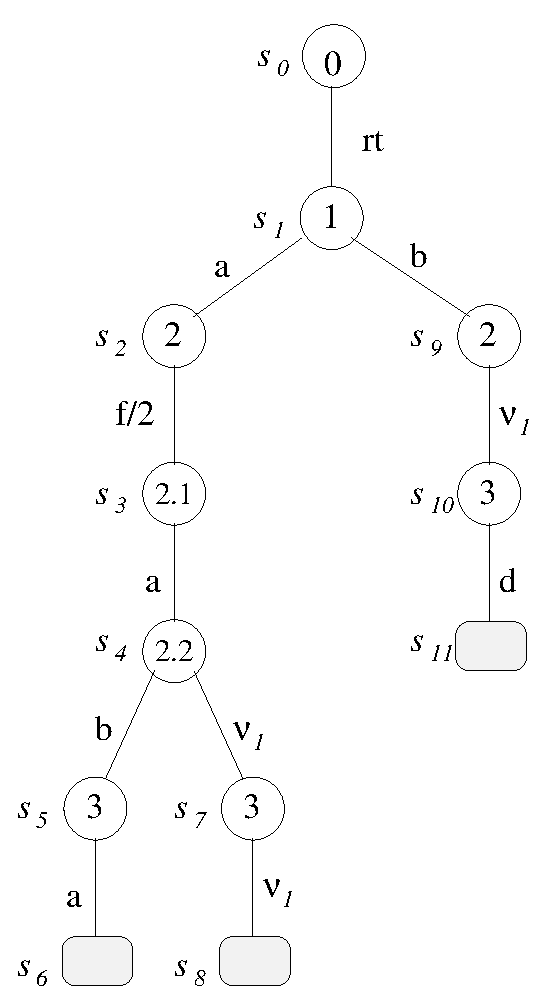
\epsfig{file=trie.eps,height=.3\textheight}
\end{tabular}
\caption{Terms Stored as a Trie}
\end{figure} 
Using a trie for storage has the advantage that discrimination can be
made on a position anywhere in a fact, and directly inserting into or
deleting from a trie is 4-5x faster than with standard dynamic code.
In addition, in trie-dynamic code, there is no distinction between the
index and the code itself, so for many sets of facts trie storage can
use much less space than standard dynamic code.  For instance,
Figure~\ref{fig:trie} shows how the prefix {\tt rt(a,f(a,...} is
shared for the first two facts.  However, trie storage comes with
tradeoffs: first, only facts can be stored in a trie; second, unlike
standard dynamic code, no ordering is preserved among the facts; and
third, duplicate facts are not supported.

In \version{} of XSB, tries that store facts may have the following
forms~\footnote{Future versions may support more types of tries}:
%
\bi
\item {\em Private, general} tries allow arbitrary terms to be
  inserted in a trie.  These tries are thread-private so that
  inserting a term in a trie $Tr$ in one thread will not be visible to
  another thread.  Although such tries are general, they have
  limitations in memory reclamation in \version{} of XSB.  If a term
  is deleted from $Tr$, memory will be reclaimed if it is safe to do
  so at the time of deletion~\footnote{That is, if no choice points
    are around that may cause backtracking into $Tr$.}; otherwise the
  will not be reclaimed until all terms in $Tr$ are removed by
  truncating $Tr$ or until the thread exits.

\item {\em Private, associative} Associative tries are more restricted
  than general tries: an associative trie combines a {\em key} which
  can be any ground term, with a {\em value} which can be any term.
  Memory for deleted key-value pairs in an associative trie is always
  immediately reclaimed, and insert or delete operations can be faster
  for an associative trie than for a general trie.  These tries are
  private to a thread, and in addition to reclaiming memory when a
  term is deleted, memory is reclaimed when the trie is truncated or
  dropped, and when the thread exits.

\item {\em Shared, associative} tries are associative tries that are
  shared among threads.  Memory for deleted key-value pairs is always
  immediately reclaimed, and xbwhen the trie is truncated or dropped.
\ei

\section{Examples of Using Tries}

A handle for a trie can be obtained using the {\tt trie\_create/2}
predicate.  Terms can then be inserted into or deleted from that trie,
and terms can be unified with information in the trie, as shown in the
following example:

\begin{example} \rm
First, we create a private general trie: 
{\small
\begin{verbatim}
| ?- trie_create(X,[type(prge)]).
X = 1

yes
\end{verbatim}
}
%
Next, we insert some terms into the trie
{\small
\begin{verbatim}
| ?- trie_insert(1,f(a,b)), trie_insert(1,[a,dog,walks]).

yes
\end{verbatim}
}
Now we can make arbitrary queries against the trie
{\small
\begin{verbatim}
| ?- trie_unify(1,X).

X = [a,dog,walks];

X = f(a,b);

no
\end{verbatim}
}
\noindent
Above, a general query was made, but the query could have been any
Prolog term.  Now we delete a term, and see what's left.
{\small
\begin{verbatim}
| ?- trie_delete(1,f(X,B)).

X = a
B = b

yes
| ?- trie_unify(1,X).

X = [a,dog,walks];

no
\end{verbatim}
}
\end{example}

The behavior of general tries can be constrasted with that of
associative tries as seen in the next example.
\begin{example} \rm
Now we start by creating a shared associative trie, with abbreviation
{\tt shas} using the multi-threaded engine
{\small
\begin{verbatim}
| ?- trie_create(X,[type(shas),alias(foo)]).
X = 1048577

yes
\end{verbatim}
}  \noindent
%
This time we used an alias so now we can use {\tt foo} to refer to
insert a couple of key-value pairs into the trie (we could also use
the trie handle itself) 
{\small
\begin{verbatim}
| ?- trie_insert(foo,pair(sentence(1),[a,dog,walks])), 
     trie_insert(foo,pair(sentence(2),[a,man,snores])).

yes
\end{verbatim}
} \noindent
However, inserting a general term into an associative trie throws an
error
{\small
\begin{verbatim}
| ?- trie_insert(foo,f(a,b)).
++Error[XSB/Runtime/P]: [Domain (f(a,b) not in domain pair/2)]  in arg 2 of pre\
dicate trie_insert/2 (Inserted term must be key-value pair in trie 1048577)
\end{verbatim}
}  \noindent
Finally, in an associative trie, if we insert a value for a key that
is already in the trie, it will {\em update} the value for that key.
{\small
\begin{verbatim}
| ?- trie_insert(foo,pair(sentence(1),[a,dog,snoress])).

yes
| ?- trie_unify(foo,pair(sentence(1),X)).
X = [a,dog,snores]

yes
\end{verbatim}
}

\end{example}

\section{Predicates for Tries} 
%
The following subsections describe predicates for inserting terms into
a trie, deleting terms from a trie, and unifying a term with terms in
a trie, further predicates for creating, dropping, and truncating
tries, as well as predicates for bulk insertes into and deletes from a
trie.  These predicates can apply to any type of trie, and perform
full error checking on their call arguments.  As such, they are safer
and more general than the lower-level trie predicates described in
Chapter 1 of Volume 2 of this manual.  Use of the predicates described
here is recommended for applications unless the need for speed is
paramount.

\begin{description}
%
\ouritem{trie\_create(-TrieId,+OptionList)}
\index{\texttt{trie\_create/2}}
%
{\tt OptionList} allows optional parameters in the configuration of a
trie to indicate its type and whether an alias should be used.  In the
present version of  
\bi
\item {\tt Type} can be one of
\bi
\item {\tt prge} (private, general) maintains information that is
  accessable only to the calling thread.  No other restrictions are
  made for accessing information in a private trie.  In the
  single-threaded engine, tries are private by default.

\item {\tt pras} (private, associative) creates a private trie that
  maintains key-value pairs in a manner similar to an associative
  array, using the term {\tt pair(Key,Value)}.  Each key must be ground,
  and there may be only one value per key.

\item {\tt shas} (shared associative) creates a shared trie that
  maintains key-value pairs in a manner similar to an associative
  array, using the term {\tt pair(Key,Value)}.  Each key must be
  ground, and there may be only one value per key.  This option is
  available only in the multi-threaded engine

%\item {\tt shared(full)} Maintains information that is accessable to
%  all threads, with no restrictions on its access.  In the
%  single-threaded engine, there is no distinction between private and
%  shared tries.
\ei
\item {\tt alias(Alias)}: Allow trie {\tt TrieId} to be referred to
  via {\tt Alias} in all standard trie predicates.  {\tt Alias}
  remains active for {\tt TrieId} until it is dropped.
\ei
%
{\bf Error Cases}
\bi
\item 	{\tt TrieId} is not a variable
\bi
\item 	{\tt type\_error(variable,TrieId)}
\ei
\item 	{\tt OptionList} is a partial list or contains an option that is a variable
\bi
\item 	{\tt instantiation\_error}
\ei
\item 	{\tt OptionList} is neither a list nor a partial list
\bi
\item 	{\tt type\_error(list,OptionsList)}
\ei
\item 	{\tt OptionList} contains an option, {\tt Option} not described above
\bi
\item 	{\tt domain\_error(trie\_option,Option)}
\ei
\item An element of {\tt OptionsList} is alias(A) and A is already
  associated with an existing thread, queue, mutex or stream 
\bi
\item {\tt permission\_error(create,alias, A)}
\ei
\item An element of {\tt OptionsList} is alias(A) and A its not an atom
\bi
\item {\tt type\_error(atom,A)}
\ei
\ei

\ouritem{trie\_insert(+TrieIdOrAlias,Term)}
\index{\texttt{trie\_insert/2}} 
%
Inserts {\tt Term} into the trie denoted by {\tt TrieIdOrAlias}.  If
{\tt TrieIdOrAlias} denotes an associative trie, {\tt Term} must be of
the form {\tt pair(Key,Value)} where {\tt Key} is ground.  If {\tt
  TrieIdOrAlias} is a general trie and already contains {\tt Term},
the predicate fails (as the same term cannot be inserted multiple
times in the same trie).  Similarly, if {\tt TrieIdOrAlias} is an
associative trie and already contains a value for {\tt Key} the
predicate fails.

{\bf Error Cases}
\bi
\item 	{\tt TrieIdOrAlias} is a variable
\bi
\item 	{\tt instantiation\_error}.
\ei
\item 	{\tt TrieIdOrAlias} is not a trie id or alias
\bi
\item 	{\tt domain\_error(trie\_id\_or\_alias,TrieIdOrAlias)}
\ei
\item 	{\tt TrieIdOrAlias} denotes an associative array, and {\tt Term} 
  does not unify with {\tt pair(\_,\_)} 
\bi
\item 	{\tt domain\_error(pair/2,Term)}
\ei
\item 	{\tt TrieIdOrAlias} denotes an associative array, 
  {\tt Term = pair(Key,Value)} but {\tt Key} is not ground 
\bi
\item 	{\tt misc\_error}
\ei
\ei
%

\ouritem{trie\_unify(+TrieIdOrAlias,Term)}
\index{\texttt{trie\_unify/2}} 
%
Unifies {\tt Term} with a term in the trie denoted by {\tt
  TrieIdOrAlias}.  If {\tt TrieIdOrAlias} denotes a general trie,
successive unifications will succeed upon backtracking.  If {\tt
  TrieIdOrAlias} denotes an associative trie, {\tt Term} must be of
the form {\tt pair(Key,Value)} where {\tt Key} is ground.

{\bf Error Cases}
\bi
\item 	{\tt TrieIdOrAlias} is a variable
\bi
\item 	{\tt instantiation\_error}.
\ei
\item 	{\tt TrieIdOrAlias} is not a trie id or alias
\bi
\item 	{\tt domain\_error(trie\_id\_or\_alias,TrieIdOrAlias)}
\ei
\item 	{\tt TrieIdOrAlias} denotes an associative array, and {\tt Term} 
  does not unify with {\tt pair(\_,\_)} 
\bi
\item 	{\tt domain\_error(pair/2,Term)}
\ei
\item {\tt TrieIdOrAlias} denotes an associative array, 
  {\tt Term = pair(Key,Value)} but {\tt Key} is not ground 
\bi
\item 	{\tt misc\_error}
\ei
\ei

\ouritem{trie\_delete(+TrieIdOrAlias,Term)}
\index{\texttt{trie\_delete/2}}
%
Deletes a term unifying with {\tt Term} from the trie denoted by {\tt
  TrieIdOrAlias}.  {\tt TrieIdOrAlias} denotes a general trie, all
such terms can be deleted upon backtracking.  If {\tt TrieIdOrAlias}
denotes an associative trie, {\tt Term} must be of the form {\tt
  pair(Key,Value)} where {\tt Key} is ground.  In either case, if {\tt
  TrieIdOrAlias} does not contain a term unifying with {\tt Term} the
preicate fails.

{\bf Error Cases}
\bi
\item 	{\tt TrieIdOrAlias} is a variable
\bi
\item 	{\tt instantiation\_error}.
\ei
\item 	{\tt TrieIdOrAlias} is not a trie id or alias
\bi
\item 	{\tt domain\_error(trie\_id\_or\_alias,TrieIdOrAlias)}
\ei
\item 	{\tt TrieIdOrAlias} denotes an associative array, and {\tt Term} 
  does not unify with {\tt pair(\_,\_)} 
\bi
\item 	{\tt domain\_error(pair/2,Term)}
\ei
\item {\tt TrieIdOrAlias} denotes an associative array, 
  {\tt Term = pair(Key,Value)} but {\tt Key} is not ground 
\bi
\item 	{\tt misc\_error}
\ei
\ei
%
\ouritem{trie\_truncate(+TrieIdOrAlias)}
\index{\texttt{trie\_truncate/1}}
%
Removes all terms from {\tt TrieIdOrAlias}, but does not change any of
its properties (e.g. the type of the trie or its aliases).  

{\bf Error Cases}
\bi
\item 	{\tt TrieIdOrAlias} is a variable
\bi
\item 	{\tt instantiation\_error}.
\ei
\item 	{\tt TrieIdOrAlias} is not a trie id or alias
\bi
\item 	{\tt domain\_error(trie\_id\_or\_alias,TrieIdOrAlias)}
\ei
\ei

\ouritem{trie\_drop(+TrieIdOrAlias)}
\index{\texttt{trie\_drop/1}}
%
Drops {\tt TrieIdOrAlias}.  {\tt trie\_drop/1} not only removes all
terms from {\tt TrieIdOrAlias}, but also removes information about its
type and any aliases the trie may have.

{\bf Error Cases}
\bi
\item 	{\tt TrieIdOrAlias} is a variable
\bi
\item 	{\tt instantiation\_error}.
\ei
\item 	{\tt TrieIdOrAlias} is not a trie id or alias
\bi
\item 	{\tt domain\_error(trie\_id\_or\_alias,TrieIdOrAlias)}
\ei
\ei

\ourmoditem{trie\_bulk\_insert(+TrieIdOrAlias,+Generator)}{intern}
\index{\texttt{trie\_bulk\_insert/2}}
% 
Used to insert multiple terms into the trie denoted by {\tt
  TrieIdOrAlias}.  {\tt Generator} must be a callable term.  Upon
backtracking through {\tt Generator} its first argument should
successively be instantiated to the terms to be interned in {\tt
  TrieIdOrAlias}.  When inserting many terms into a general trie, {\tt
  trie\_bulk\_insert/2} is faster than repeated calls to {\tt
  trie\_insert/2} as it does not need to make multiple checks that the
choice point stack is free of failure continuations that point into
the {\tt TrieIdOrAlias} trie.  For associative tries, {\tt
  trie\_bulk\_insert/2} can also be faster as it needs to perform
fewer error checks on the arguments of the insert.

\begin{example} \rm
Given the predicate 
\begin{verbatim}
bulk_create(p(One,Two,Three),N):- 
     for(One,1,N),
     for(Two,1,N),
     for(Three,1,N).
\end{verbatim}
and a general trie {\tt Trie}, the goal 
\begin{center}
   {\tt ?- trie\_bulk\_insert(Trie,bulk\_create(\_Term,N))} 
\end{center}
will add $N^3$ terms to {\tt Trie}.
\end{example}

{\bf Error Cases}
\bi
\item 	{\tt TrieIdOrAlias} is a variable
\bi
\item 	{\tt instantiation\_error}.
\ei
\item 	{\tt TrieIdOrAlias} is not a trie id or alias
\bi
\item 	{\tt domain\_error(trie\_id\_or\_alias,TrieIdOrAlias)}
\ei
\item   {\tt Generator} is not a compound term
\bi
\item   {\tt type\_error(compound,Generator)}
\ei
\item 	{\tt TrieIdOrAlias} denotes an associative array, and {\tt Generator} 
  does not unify with {\tt pair(\_,\_)} 
\bi
\item 	{\tt domain\_error(pair/2,Term)}
\ei
\item {\tt TrieIdOrAlias} denotes an associative array, and {\tt
  Generator} succeeds with a term that unifies with {\tt
  pair(Key,Value)} and {\tt Key} is not ground 
\bi
\item 	{\tt misc\_error}
\ei
\ei

\ourmoditem{trie\_bulk\_delete(+TrieIdOrAlias,Term)}{intern}
\index{\texttt{trie\_bulk\_delete/2}}
% 
Deletes all terms that unify with {\tt Term} from {\tt TrieIdOrAlias}.
If {\tt TrieIdOrAlias} denotes an associative trie, the key of the key
value pair need {\em not} be ground.

\begin{example}\label{ex:bulk-delete} \rm
For the trie in the previous example, the goal 
\begin{center}
{\tt ?-  trie\_bulk\_delete(Trie,p(1,\_,\_))} 
\end{center}
will delete the $N^2$ terms that unify with {\tt p(1,\_,\_)} from {\tt TrieIdOrAlias}.
\end{example}

{\bf Error Cases}
\bi
\item 	{\tt TrieIdOrAlias} is a variable
\bi
\item 	{\tt instantiation\_error}.
\ei
\item 	{\tt TrieIdOrAlias} is not a trie id or alias
\bi
\item 	{\tt domain\_error(trie\_id\_or\_alias,TrieIdOrAlias)}
\ei
\ei

\ourmoditem{trie\_bulk\_unify(+TrieIdOrAlias,\#Term,-List)}{intern}
\index{\texttt{trie\_bulk\_unify/3}}
% 
Returns in {\tt List} all terms in {\tt TrieIdOrAlias} that unify with
{\tt Term}.  If {\tt TrieIdOrAlias} denotes an associative trie, the
key of the key value pair need {\em not} be ground.

This predicate is useful for two reasons.  First, it provides a safe
way to backtrack through an associative trie while maintaining the
memory management and concurrency properties of associative tries.
Second, it enforces read consistency for {\tt TrieIdOrAlias},
regardless of whether the trie is private or shared, general or
associative.

\begin{example} \rm
Continuing from Example~\ref{ex:bulk-delete} the goal
\begin{center}
{\tt ?-  trie\_bulk\_unify(Trie,X),List} 
\end{center}
will return the the $N^3 - N^2$ terms still in {\tt TrieIdOrAlias}.
\end{example}

{\bf Error Cases}
\bi
\item 	{\tt TrieIdOrAlias} is a variable
\bi
\item 	{\tt instantiation\_error}.
\ei
\item 	{\tt TrieIdOrAlias} is not a trie id or alias
\bi
\item 	{\tt domain\_error(trie\_id\_or\_alias,TrieIdOrAlias)}
\ei
\item 	{\tt List} is not a variable
\bi
\item 	{\tt type\_error(variable,List)}.
\ei
\ei

\ouritem{trie\_property(?TrieOrAlias,?Property)}
\index{\texttt{trie\_property/2}} 
%
If {\tt TrieOrAlias} is instantiated, unifies {\tt Property} with
current properties of the trie; if {\tt TrieOrAlias} is a variable,
backtracks through all the current tries whose properties unify with
{\tt Property}.  In the MT engine, {\tt thread\_property/2} accesses
only tries private to the calling thread and shared tries; however
note that there is no guarantee that that the information returned
about shared tries will be valid, due to concurrency
issues~\footnote{{\tt trie\_property/2} is not yet implemented for
  shared tries.}.

Currently {\tt Property} can have the form 
\bi
\item {\tt type(Type)}: where {\tt Type} is the type of the trie.
%
\item {\tt alias(Alias)}: if the trie has an alias {\tt Alias}
\ei

{\bf Error Cases}
%
\bi
\item {\tt TrieOrAlias} is neither a variable nor an XSB trie id
  nor an alias
\bi
\item {\tt domain\_error(trie, TrieOrAlias)}
\ei
\item {\tt TrieOrAlias} is not associated with a valid trie
\bi
\item {\tt existence\_error(trie, TrieOrAlias)}
\ei
\ei

%\ouritem{trie\_property(+TrieIdOrAlias,Property)}
%\index{\texttt{trie\_property/2}}
%
\end{description}


\chapter{Hooks} \label{hooks}

Sometimes it is useful to let the user application catch certain
events that occur during XSB execution. For instance, when the user
asserts or retracts a clause, etc.  XSB has a general mechanism by
which the user program can register \emph{hooks} to handle certain
supported events. All the predicates described below must be imported
from {\tt xsb\_hook}.


\section{Adding and Removing Hooks}

A hook in XSB can be either a 0-ary predicate or a unary predicate.
A 0-ary hook is called without parameters and unary hooks are called with
one parameter. The nature of the parameter depends on the type of the hook,
as described in the next subsection.


\begin{description}
\ourmoditem{add\_xsb\_hook(+HookSpec)}{add\_xsb\_hook/1}{xsb\_hook}

This predicate registers a hook; it must be imported from {\tt xsb\_hook}.
{\tt HookSpec} has the following format:
%%
\begin{quote}
 {\tt
   hook-type(your-hook-predicate(\_))
   }
\end{quote}
%%
or, if it is a 0-ary hook:
%%
\begin{quote}
  {\tt
   hook-type(your-hook-predicate)
   }  
\end{quote}
%%
For instance, 
%%
\begin{verbatim}
    :- add_xsb_hook(xsb_assert_hook(foobar(_))).
\end{verbatim}
%%
registers the hook {\tt foobar/1} as a hook to be called when XSB
asserts a clause. Your program must include
clauses that define {\tt foobar/1}, or else an error will result.

The predicate that defines the hook type must be imported from {\tt
  xsb\_hook}:
%%
\begin{verbatim}
    :- import xsb_assert_hook/1 from xsb_hook.  
\end{verbatim}
%%
or {\tt add\_xsb\_hook/1} will issue an error.

\ourmoditem{remove\_xsb\_hook(+HookSpec)}{remove\_xsb\_hook/1}{xsb\_hook}

Unregisters the specified XSB hook; imported from {\tt xsb\_hook}. For
instance,
%%
\begin{verbatim}
    :- remove_xsb_hook(xsb_assert_hook(foobar(_))).
\end{verbatim}
%%
As before, the predicate that defines the hook type must be imported from
{\tt xsb\_hook}.
\end{description}


\section{Hooks Supported by XSB}

The following predicates define the hook types supported by XSB. They must
be imported from {\tt xsb\_hook}.

\begin{description}
\ourmoditem{xsb\_exit\_hook(\_)}{xsb\_exit\_hook/1}{xsb\_hook} 

These hooks are called just before XSB exits. You can register as many
hooks as you want and all of them will be called on exit (but the order of
the calls is not guaranteed). Exit hooks are all 0-ary and must be registered
as such:
%%
\begin{verbatim}
    :- add_xsb_hook(xsb_exit_hook(my_own_exit_hook)).
\end{verbatim}
%%


\ourmoditem{xsb\_assert\_hook(\_)}{xsb\_assert\_hook/1}{xsb\_hook} 
%
These hooks are called whenever the program asserts a clause. An assert
hook must be a unary predicate, which expects the clause
being asserted as a parameter. For instance,
%%
\begin{verbatim}
    :- add_xsb_hook(xsb_assert_hook(my_assert_hook(_))).
\end{verbatim}
%%
registers {\tt my\_assert\_hook/1} as an assert hook. One can register
several assert hooks and all of them will be called (but the order is not
guaranteed).

\ourmoditem{xsb\_retract\_hook(\_)}{xsb\_retract\_hook/1}{xsb\_hook} 
%
These hooks are called whenever the program retracts a clause. A retract
hook must be a unary predicate, which expects as a parameter a list of the
form {\tt [Head,Body]}, which represent the head and the body parts of the
clause being retracted. As with assert hooks, any number of retract hooks
can be registered and all of them will be called in some order.

\end{description}


%%% Local Variables: 
%%% mode: latex
%%% TeX-master: "manual1"
%%% End: 

\chapter{Debugging} \label{debugging}
%====================================
\index{debugger}

\section{High-Level Tracing}
%===========================
\index{high-level tracing}
\index{tracing!high-level}

\ourprolog\ supports a version of the Byrd four-port debugger for debugging
Prolog code.  In this release (\version), it does not work very well
when debugging code involving tabled predicates.  If one only creeps
(see below), the tracing can provide some useful information.  We do
intend that future versions will have more complete debugging help for
tabled evaluation.

To turn on tracing, use {\tt trace/0}.  To turn tracing off, use 
{\tt notrace/0}.  When tracing is on, the system will print a message each
time a predicate is:
\begin{enumerate} \index{debugger!ports}
\item initially entered (Call), 
\item successfully returned from (Exit), 
\item failed back into (Redo), and
\item completely failed out of (Fail).  
\end{enumerate}
At each port, a message is printed and the tracer stops and prompts
for input.  (See the predicates {\tt show/1} and {\tt leash/1} described
below to modify what is traced and when the user is prompted.)

In addition to single-step tracing, the user can set spy points to influence
how the tracing/debugging works.  A spy point is set using {\tt spy/1}.
Spy points can be used to cause the system to enter the tracer when
a particular predicate is entered. Also the tracer allows ``leaping'' from
spy point to spy point during the debugging process.

When the tracer prompts for input, the user may enter a return, or a single
character followed by a return, with the following meanings:
\index{trace!options}
\begin{description}
\item[{\tt c, <CR>}: Creep]
    Causes the system to single-step to the next port
    (i.e.\ either the entry to a traced predicate called by the executed clause,
    or the success or failure exit from that clause).
\item[{\tt a}: Abort]\index{abort!trace facility}
    Causes execution to abort and control to return to the top level
    interpreter.
\item[{\tt b}: Break]
    Calls the evaluable predicate {\em break}, thus invoking recursively
    a new incarnation of the system interpreter.
    The command prompt at break level $n$ is
    \begin{center}
    {\tt $n$: \tt ?-}
    \end{center}
    The user may return to the previous break level by entering the system
    end-of-file character (e.g.\ {\tt ctrl-D}), or typing in the atom 
    {\tt end\_of\_file}; or to the top level interpreter by typing in
    {\tt abort}.
\item[{\tt f}: Fail] Causes execution to fail, thus transferring control to
    the Fail port of the current execution.
\item[{\tt h}: Help] Displays the table of debugging options.
\item[{\tt l}: Leap] Causes the system to resume running the program,
    only stopping when a spy-point is reached or the program terminates.
    This allows the user to follow the execution at a higher level than
    exhaustive tracing.
\item[{\tt n}: Nodebug] Turns off debug mode.
\item[{\tt q}: Quasi-skip] This is like Skip except that it does not mask
    out spy points.
\item[{\tt r}: Retry (fail)] Transfers to the Call port of the current goal.
    Note, however, that side effects, such as database modifications etc.,
    are not undone.
\item[{\tt s}: Skip] Causes tracing to be turned off for the entire execution
    of the procedure.  Thus, nothing is seen until control comes back to that
    procedure, either at the Success or the Failure port.
\item[{\tt e}: Exit] Causes immediate exit from \ourprolog\ back to the
    operating system.
\end{description}

Other standard predicates that are useful in debugging are:

\begin{description}
\ouritem{spy(Preds)} \index{{\tt spy/1}}
%\predindex{spy/1~(L)}
    where {\tt Preds} is a spy specification or a list of such
    specifications, and must be instantiated. This predicate sets spy
    points (conditional or unconditional) on predicates.  A spy
    specification can be of several forms. Most simply, it is a term
    of the form $P$/$N$, where $P$ is a predicate name and $N$ its
    arity.  Optionally, only a predicate name can be provided, in
    which case it refers to all predicates of any arity currently
    defined in {\tt usermod}.  It may optionally may be prefixed by a
    module name, e.g.  $ModName$:$P$/$N$. (Again, if the arity is
    omitted, the specifaction refers to all predicates of any arity
    with the given name currently defined in the given module.)  A spy
    specification may also indicate a conditional spy point. A
    conditional spy specification is a Prolog rule, the head
    indicating the predicate to spy, and the body indicating
    conditions under which to spy. For example, to spy the predicate
    p/2 when the first argument is not a variable, one would write:
    $spy (p(X,\_):-nonvar(X)).$ (Notice that the parentheses around
    the rule are necessary). The body may be empty, i.e., the rule may
    just be a fact.  The head of a rule may also be prefixed (using
    $:$) with a module name. One should not put both conditional and
    unconditional spy points on the same predicate.

\ouritem{nospy(Preds)} \index{{\tt nospy/1}}
%\predindex{nospy/1~(L)}
    where {\tt Preds} is a spy specification, or a list of such
    specifications, and must be instantiated at the time of call.  What
    constitutes a spy specification is described above under {\tt spy}.
    {\tt nospy} removes spy points on the specified predicates. If a
    specification is given in the form of a fact, all conditional spy points
    whose heads match that fact are removed.

\ouritem{debug} \index{{\tt debug/0}} 
%\predindex{debug/0~(L)}
    Turns on debugging mode.
    This causes subsequent execution of predicates with trace or spy
    points to be traced, and is a no-op if there are no such predicates.
    The predicates {\tt trace/1} and {\tt spy/1} cause debugging mode
    to be turned on automatically.

\ouritem{nodebug} \index{{\tt nodebug/0}}
%\predindex{nodebug/0~(L)}
    Turns off debugging mode.  This causes trace and spy points to be ignored.

\ouritem{debugging} \index{{\tt debugging/0}}
%\predindex{debugging/0~(L)}
    Displays information about whether debug mode is on or not, and lists
    predicates that have trace points or spy points set on them.

\ouritem{show(PortList)} \index{{\tt show/1}}
%\predindex{show/1~(L)}
    Allows the user to specify at which ports should trace messages be
    printed. {\tt PortList} must be a list of port names, i.e., a sublist
    of ['Call', 'Exit', 'Redo', 'Fail']. {\tt show/1} is not a standard
    predicate but must be imported from the module {\tt debugger} before
    it can be called.

\ouritem{leash(PortList)} \index{{\tt leash/1}}
%\predindex{leash/1~(L)}
    Allows the user to specify at which ports the tracer should stop
    and prompt the user for direction.  {\tt PortList} must be a list of
    port names, i.e., a sublist of ['Call', 'Exit', 'Redo', 'Fail'].  Only
    ports that are {\tt show}-n can be {\tt leash}-ed.  {\tt leash/1} is
    not a standard predicate but must be imported from the module {\tt
    debugger} before it can be called.
\end{description}


\section{Low-Level Tracing}
%--------------------------------------------------
\index{low-level tracing} \index{tracing!low-level}

\ourprolog\ also provides a facility for low-level tracing of execution.
This can be activated by invoking the emulator with the {\tt -T} option
(see section~\ref{emulator_options}), or through the predicate {\tt trace/0}.
\index{\$trace/0} %\predindex{\$trace/0~(L)}
It causes trace information to be printed out at every call (including
those to system trap handlers).  The volume of such trace information
can very become large very quickly, so this method of tracing is not
recommended in general.


%%% Local Variables: 
%%% mode: latex
%%% TeX-master: "manual"
%%% End: 

\chapter{Definite Clause Grammars} \label{DCGs}
\index{definite clause grammars}\index{grammars!definite clause}
%===============================================================

\section{General Description}
%============================

Definite clause grammars (DCGs) are an extension of context free
grammars that have proven useful for describing natural and formal
languages, and that may be conveniently expressed and executed in
Prolog.  A Definite Clause Grammar rule is executable because it is
just a notational variant of a logic rule that has the following
general form:
\begin{center}
                {\em Head} {\tt -->} {\em Body.}
\end{center}
with the declarative interpretation that ``a possible form for {\em
Head} is {\em Body}''. The procedural interpretation of a grammar rule
is that it takes an input sequence of symbols or character codes,
analyses some initial portion of that list, and produces the remaining
portion (possibly enlarged) as output for further analysis.  In XSB,
the exact form of this sequence is determined by whether XSB's {\em
DCG mode} is set to use tabling or not, as will be discussed below.
In either case, the arguments required for the input and output lists
are not written explicitly in the DCG rule, but are added when the
rule is translated (expanded) into an ordinary normal rule during
parsing.  Extra conditions, in the form of explicit Prolog literals or
control constructs such as {\em if-then-elses} ({\tt '->'/2}) or {\em
cuts}\index{cut} (\cut)\index{\texttt{"!/0}}, may be included in the {\em
Body} of the DCG rule and they work exactly as one would expect.

The syntax of DCGs is orthogonal to whether tabling is used for DCGs
or not.  An overview of DCG syntax
 supported by XSB is as follows:
\begin{enumerate}
\item A non-terminal symbol may be any HiLog term other than a variable
      or a number. A variable which appears in the body of a rule is
      equivalent to the appearance of a call to the standard predicate
      {\tt phrase/3} as it is described below.
\item A terminal symbol may be any HiLog term. In order to distinguish 
      terminals from nonterminals, a sequence of one or more terminal
      symbols   $\alpha, \beta, \gamma, \delta, \ldots$
      is written within a grammar rule as a Prolog list 
         {\tt [} $\alpha, \beta, \gamma, \delta, \ldots$ {\tt ]},
      with the empty sequence written as the empty list {\tt [\,]}.
      The list of terminals may contain variables but it has to be a 
      proper list, or else an error message is sent to the standard 
      error stream and the expansion of the grammar rule that contains 
      this list will fail. If the terminal symbols are ASCII character
      codes, they can be written (as elsewhere) as strings.
\item Extra conditions, expressed in the form of Prolog predicate calls, 
      can be included in the body (right-hand side) of a grammar rule by 
      enclosing such conditions in curly brackets, {\tt '$\{$'} and
      {\tt '$\}$'}.
      For example, one can write:
      \begin{center}
                {\tt positive\_integer(N) --> [N], $\{$integer(N), N > 0$\}$.}
                \footnote{A term like {\tt $\{$foo$\}$} is just a
			  syntactic-sugar for the term {\tt '$\{\}$'(foo)}.}
      \end{center}
\item The left hand side of a DCG rule must consist of a single non-terminal,
      possibly followed by a sequence of terminals (which must be written as
      a {\em unique} Prolog list). Thus in XSB, unlike SB-Prolog 
      version 3.1, ``push-back lists'' are supported.
\item The right hand side of a DCG rule may contain alternatives (written 
      using the usual Prolog's disjunction operator {\tt ';'} or 
      using the usual BNF disjunction operator {\tt '|'}. 
\item The Prolog control primitives {\em if-then-else} ({\tt '->'/2}),
      {\em nots} ({\tt not/1, fail\_if/1}, \not\ or {\tt tnot/1}) and 
      {\em cut}\index{cut} (\cut)\index{\texttt{"!/0}} may also be included in the 
      right hand side of a DCG rule. These symbols need not be enclosed in 
      curly brackets. 
      \footnote{Readers familiar with Quintus Prolog may notice the difference
                in the treatment of the various kinds of not. For example, in 
                Quintus Prolog a {\tt not/1} that is not enclosed within curly 
                brackets is interpreted as a non-terminal grammar symbol.}
      All other Prolog's control primitives, such as {\tt repeat/0}, must
      be enclosed explicitly within curly brackets if they are not meant
      to be interpreted as non-terminal grammar symbols.
\end{enumerate}
 

\section{Translation of Definite Clause Grammar rules}
%=====================================================

In this section we informally describe the translation of DCG rules
into normal rules in XSB.  Each grammar rule is translated into a
Prolog clause as it is consulted or compiled.  This is accomplished
through a general mechanism of defining the hook predicate {\tt
term\_expansion/2}, \stdrefindex{term\_expansion/2} by means of which
a user can specify any desired transformation to be done as clauses
are read by the reader of XSB's parser.  This DCG term expansion is as
follows:

A DCG rule such as:

\stuff{
\> \> p(X) --> q(X).
}

\noindent
will be translated (expanded) into:

\stuff{
\> \> p(X, Li, Lo) :- \\ 
\> \> \>  q(X, Li, Lo).
}

If there is more than one non-terminal on the right-hand side, as in

\stuff{\> \> p(X, Y) --> q(X), r(X, Y), s(Y).}

\noindent
the corresponding input and output arguments are identified, 
translating into:

\stuff{
\> \> p(X, Y, Li, Lo) :- \\ 
\> \> \> q(X, Li, L1), \\
\> \> \> r(X, Y, L1, L2), \\
\> \> \> s(Y, L2, Lo).
}

Terminals are translated using the predicate {\tt 'C'/3} (See 
section~\ref{DCG_builtins} for its description).  For instance:

\stuff{\> \> p(X) --> [go, to], q(X), [stop].}

\noindent
is translated into:

\stuff{  
\> \> p(X, S0, S) :- \\
\> \> \> 'C'(S0, go, S1), \\
\> \> \> 'C'(S1, to, S2), \\
\> \> \> q(X, S2, S3), \\
\> \> \> 'C'(S3, stop, S).
}

Extra conditions expressed as explicit procedure calls naturally translate
into themselves. For example,

\stuff{
\> \> positive\_number(X) --> \\
\> \> \> [N], $\{$integer(N), N > 0$\}$, \\
\> \> \> fraction(F), $\{$form\_number(N, F, X)$\}$.}

\noindent
translates to:

\stuff{
\> \> positive\_number(X, Li, Lo) :- \\
\> \> \> 'C'(Li, N, L1), \\
\> \> \> integer(N), \\
\> \> \> N > 0, \\
\> \> \> L1 = L2, \\
\> \> \> fraction(F, L2, L3), \\
\> \> \> form\_number(N, F, N), \\
\> \> \> L3 = Lo. \\
}

Similarly, a cut is translated literally.

{\em Push-back lists} (a proper list of terminals on the left-hand side of 
a DCG rule) translate into a sequence of {\tt 'C'/3} goals with the first 
and third arguments reversed.
For example,

\stuff{\> \> it\_is(X), [is, not] --> [aint].}

\noindent
becomes

\stuff{
\> \> it\_is(X, Li, Lo) :- \\
\> \> \> 'C'(Li, aint, L1), \\
\> \> \> 'C'(Lo, is, L2), \\
\> \> \> 'C'(L2, not, L1).
}

Disjunction has a fairly obvious translation.  For example, the DCG clause:

\stuff{
\> \> expr(E) --> \\
\> \> \> \ \ expr(X), "+", term(Y), $\{$E is X+Y$\}$ \\
\> \> \>   | term(E).
}

\noindent
translates to the Prolog rule:

\stuff{
\> \>expr(E, Li, Lo) :- \\
\> \> \>   ( expr(X, Li, L1), \\
\> \> \> \ \ 'C'(L1, 43, L2), \> \% 0'+ = 43 \\
\> \> \> \ \ term(Y, L2, L3) \\
\> \> \> \ \ E is X+Y, \\
\> \> \> \ \ L3 = Lo \\
\> \> \>   ; term(E, Li, Lo) \\
\> \> \>   ).
}

\subsection{Definite Clause Grammars and Tabling}
%============================================================
\label{sec:dcg_tabling}

Tabling can be used in conjunction with Definite Clause Grammars to get the
effect of a more complete parsing strategy.  When Prolog is used to evaluate
DCG's, the resulting parsing algorithm is {\em ``recursive descent''}.
Recursive descent parsing, while efficiently implementable, is known to
suffer from several deficiencies:  1) its time can be exponential in the size
of the input, and 2) it may not terminate for certain context-free grammars (in
particular, those that are left or doubly recursive).  By appropriate use of
tabling, both of these limitations can be overcome.  With appropriate tabling,
the resulting parsing algorithm is a variant of {\em Earley's algorithm\/} and
of {\em chart parsing algorithms}.

In the simplest cases, one needs only to add the directive {\tt :-
auto\_table} (see Section~\ref{tabling_directives}) to the source file
containing a DCG specification.  This should generate any necessary
table declarations so that infinite loops are avoided (for
context-free grammars).  That is, with a {\tt :- auto\_table}
declaration, left-recursive grammars can be correctly processed.  Of
course, individual {\tt table} directives may also be used, but note
that the arity must be specified as two more than that shown in the
DCG source, to account for the extra arguments added by the expansion.
However, the efficiency of tabling for DCGs depends on the
representation of the input and output sequences used, a topic to
which we now turn.

\index{definite clause grammars!list mode}

Consider the expanded DCG rule from the previous section:

\stuff{ \>
\> p(X, S0, S) :- \\ 
\> \> \> 'C'(S0, go, S1), \\ 
\> \> \> 'C'(S1, to,S2), \\ 
\> \> \> q(X, S2, S3), \\ 
\> \> \> 'C'(S3, stop, S).  } 

In a Prolog system, each input and output variable, such as {\tt S0}
or {\tt S} is bound to a variable or a difference list.  In XSB, this
is called {\em list mode}.  Thus, to parse {\em go to lunch stop} the
phrase would be presented to the DCG rule as a list of tokens {\tt
[go,to,lunch,stop]} via a call to {\tt phrase/3} such as:

\stuff{\> \> phrase(p(X),[go,to,lunch,stop]).}

\noindent
or an explicit call to {\tt p/3}, such as:

\stuff{\> \> p(X,[go,to,lunch,stop|X],X).}

\noindent
Terminal elements of the sequence are consumed (or generated) via the
predicate {\tt 'C'/3} which is defined for Prolog systems as:

\stuff{\> \> 'C'([Token|Rest],Token,Rest).}

While such a definition would also work correctly if a DCG rule were
tabled, the need to copy sequences into or out of a table can lead to
behavior quadratic in the length of the input sequence (See Section
\ref{sec:TablingPitfalls}).  As an alternative, XSB allows a mode of
DCGs that defines {\tt 'C'/3} as a call to a Datalog predicate {\tt
word/3} \stdrefindex{word/3}:

\stuff{\> \> 'C'(Pos,Token,Next\_pos):- word(Pos,Token,Next\_pos).}

\noindent
assuming that each token of the sequence has been asserted as a {\tt
word/3} fact, e.g:

\stuff{
\> \> word(0,go,1). \\
\> \> word(1,to,2). \\
\> \> word(2,lunch,3). \\
\> \> word(3,stop,4).
}

\noindent
The above mode of executing DCGs is called {\em datalog mode}.  
\index{definite clause grammars!datalog mode}

{\tt word/3} facts are asserted via a call to the predicate {\tt
tphrase\_set\_string/1}.  Afterwards, a grammar rule can be called
either directly, or via a call to {\tt tphrase/1}.  To parse the list
{\tt [go,to,lunch,stop]} in datalog mode using the predicate {\tt p/3}
from above, the call

\stuff{\> \> tphrase\_set\_string([go,to,lunch,stop])}

\noindent
would be made, afterwards the sequence could be parsed via the goal:

\stuff{tphrase(p(X)).}

\noindent
or

\stuff{p(X,0,F).}

To summarize, DCGs in list mode have the same syntax as they do in
datalog mode: they just use a different definition of {\tt 'C'/3}.  Of
course tabled and non-tabled DCGs can use either definition of {\tt
'C'/3}.  Indeed, this property is necessary for tabled DCG predicates
to be able to call non-tabled DCG predicates and vice-versa.  At the
same time,tabled DCG rules may execute faster in datalog mode, while
non-tabled DCG rules may execute faster in list mode.

Finally, we note that the mode of DCG parsing is part of XSB's state.
XSB's default mode is to use list mode: the mode is set to datalog
mode via a call to {\tt tphrase\_set\_string/3} and back to list mode
by a call to {\tt phrase/2} or by a call to {\tt reset\_dcg\_mode/0}.

\section{Definite Clause Grammar predicates} \label{DCG_builtins}
%================================================================
The library predicates of XSB that support DCGs are the following:

\begin{description}

\standarditem{phrase(+Phrase, ?List)}{phrase/2}
    This predicate is true iff the list {\tt List} can be parsed as a phrase 
    (i.e. sequence of terminals) of type {\tt Phrase}.  {\tt Phrase} can be 
    any term which would
    be accepted as a nonterminal of the grammar (or in general, it can 
    be any  grammar rule body), and must be instantiated to a
    non-variable term  at the time of the call; otherwise an error
    message is sent to the standard error stream and the predicate fails. 
    This predicate is the usual way to commence execution of grammar rules.

    If {\tt List} is bound to a list of terminals by the time of the call,
    then the goal corresponds to parsing {\tt List} as a phrase of type
    {\tt Phrase}; otherwise if {\tt List} is unbound, then the grammar
    is being used for generation.

\standarditem{tphrase(+Phrase)}{tphrase/1} This predicate is
    succeeds if the current database of {\tt word/3} facts can be
    parsed via a call to the term expansion of {\tt +Phrase} whose
    input argument is set to {\tt 0} and whose output argument is set
    to the largest {\tt N} such that {\tt word(\_,\_,N)} is currently
    true.  

    The database of {\tt word/3} facts is assumed to have been
    previously set up via a call to {\tt tphrase\_set\_string/1} (or variant).  If
    the database of {\tt word/3} facts is empty, {\tt tphrase/1} will
    abort.

% TLS: handle error condition better in predicate.

\standarditem{phrase(+Phrase, ?List, ?Rest)}{phrase/3}
    This predicate is true iff the segment between the start of list 
    {\tt List} and the start of list {\tt Rest} can be parsed as a phrase 
    (i.e. sequence of terminals) of type {\tt Phrase} . In other words, if 
    the search for phrase 
    {\tt Phrase} is started at the beginning of list {\tt List}, then 
    {\tt Rest} is what remains unparsed after {\tt Phrase} has been
    found. Again, {\tt Phrase} can be any term which
    would be accepted as a nonterminal of the grammar (or in general, any
    grammar rule body), and must be instantiated to a non-variable term
    at the time of the call; otherwise an error message is sent to the
    standard error stream and the predicate fails.

    Predicate {\tt phrase/3} is the analogue of {\tt call/1} for grammar
    rule bodies, and provides a semantics for variables in the bodies of
    grammar rules.  A variable {\tt X} in a grammar rule body is treated
    as though {\tt phrase(X)} appeared instead, {\tt X} would expand into 
    a call to {\tt phrase(X, L, R)} for some lists {\tt L} and {\tt R}.  

\standarditem{expand\_term(+Term1, ?Term2)}{expand\_term/2} 
%
This predicate is used to transform terms that appear in a Prolog
program before the program is compiled or consulted.  The default
transformation performed by {\tt expand\_term/2} is that when {\tt
  Term1} is a grammar rule, then {\tt Term2} is the corresponding
Prolog clause; otherwise {\tt Term2} is simply {\tt Term1}
unchanged. If {\tt Term1} is not of the proper form, or {\tt Term2}
does not unify with its clausal form, predicate {\tt expand\_term/2}
simply fails.

Users may augment the default transformations by asserting clauses for
the predicate {\tt term\_expansion/2}\stdrefindex{term\_expansion/2}
to {\tt usermod}.  After {\tt term\_expansion(Term\_a,Term\_b)} is
asserted, then if a consulted file contains a clause that unifies with
{\tt Term\_a} the clause will be transformed to {\tt Term\_b} before
further compilation.  {\tt expand\_term/2} calls user clauses for {\tt
  term\_expansion/2} first; if the expansion succeeds, the transformed
term so obtained is used and the standard grammar rule expansion is
not tried; otherwise, if {\tt Term1} is a grammar rule, then it is
expanded using {\tt dcg/2}; otherwise, {\tt Term1} is used as is.
%Note that predicate {\tt term\_expansion/2} must be defined in the
%XSB's default read-in module ({\tt usermod}) and should be loaded
%there before the compilation begins.

{\bf Example:} 
%
Suppose the following clause is asserted:
%
\begin{verbatim}
?- assert(term_expansion(foo(X),bar(X))).
\end{verbatim}
and that the file {\tt te.P} contains the clause
%
{\tt foo(a)}
%
then the clause will automatically be expanded upon consulting the file:
%
\begin{verbatim}
| ?- [te].
[Compiling /Users/macuser/te]
[te compiled, cpu time used: 0.0170 seconds]
[te loaded]

yes
| ?- bar(X).

X = a

yes
| ?- foo(X).
++Error[XSB/Runtime/P]: [Existence (No procedure usermod : foo / 1 exists)] []
Forward Continuation...
\end{verbatim}

However, {\tt read/[1,2]} does not automatically perform term expansion
%
\begin{verbatim}
| ?- use_module(standard,[expand_term/2]).

yes
| ?- read(X),expand_term(X,Y).
foo(a).

X = foo(a)
Y = bar(a)

yes
\end{verbatim}




\standarditem{'C'(?L1, ?Terminal, ?L2)}{`C'/3}
This predicate generally is of no concern to the user.  Rather it is used 
    in the transformation of terminal symbols in 
    grammar rules and expresses the fact that {\tt L1} is connected 
    to {\tt L2} by the terminal {\tt Terminal}. This predicate is
    needed to avoid problems due to source-level
    transformations in the presence of control primitives such as
    {\em cuts}\index{cut} (\cut)\index{\texttt{"!/0}}, or {\em if-then-elses} 
    ({\tt '->'/2}) and is defined by the single clause:
    \begin{center}
                {\tt 'C'([Token|Tokens], Token, Tokens).}
    \end{center}
    The name 'C' was chosen for this predicate so that another useful
    name might not be preempted.

\standarditem{tphrase\_set\_string(+List)}{tphrase\_set\_string/1}
This predicate 

\begin{enumerate}
\item abolishes all tables;
\item retracts all {\tt word/3} facts from XSB's store; and
\item asserts new {\tt word/3} facts corresponding to {\tt List} as
described in Section \ref{sec:dcg_tabling}.
\end{enumerate}

\noindent
implicitly changing the DCG mode from list to datalog.

\ourmoditem{tphrase\_set\_string\_keeping\_tables(+List)}{tphrase\_set\_string\_keeping\_tables/1}{dcg}
This predicate is the same as {\tt tphrase\_set\_string}, except
it does not abolish any tables.  When using this predicate, the
user is responsible for explicitly abolishing the necessary tables.

\ourmoditem{tphrase\_set\_string\_auto\_abolish(+List)}{tphrase\_set\_string\_auto\_abolish/1}{dcg}
This predicate is the same as {\tt tphrase\_set\_string}, except
it abolishes tables that have been indicated as dcg-supported tables
by a previous call to {\tt set\_dcg\_supported\_table/1}.

\ourmoditem{set\_dcg\_supported\_table(+TabSkel)}{set\_dcg\_supported\_table/1}{dcg}
This predicate is used to indicate to the DCG subsystem that a
particular tabled predicate is part of a DCG grammar, and thus the
contents of its table depends on the string being parsed.  {\tt
TabSkel} must be the skeleton of a tabled predicate.  When {\tt
tphrase\_set\_string\_auto\_abolish/1} is called, all tables that have
been indicated as DCG-supported by a call to this predicate will be
abolished.

\ourmoditem{dcg(+DCG\_Rule, ?Prolog\_Clause)}{dcg/2}{dcg}
    Succeeds iff the DCG rule {\tt DCG\_Rule} translates to the Prolog
    clause {\tt Prolog\_Clause}.  At the time of call, {\tt DCG\_Rule}
    must be bound to a term whose principal functor is {\tt '-->'/2}
    or else the predicate fails.  {\tt dcg/2} must be explicitly
    imported from the module {\sf dcg}.

\end{description}


\section{Two differences with other Prologs}\label{sec-dcg-differences}
%===========================================
The DCG expansion provided by XSB is in certain cases different 
from the ones provided by some other Prolog systems (e.g.  Quintus Prolog, 
SICStus Prolog and C-Prolog). The most important of these differences are:
\begin{enumerate}
\item XSB expands a DCG clause in such a way that when a \cut\ is 
      the last goal of the DCG clause, the expanded DCG clause is always 
      {\em steadfast}.

      That is, the DCG clause:

      \stuff{
      \> \> a --> b, ! ; c.
      }

      \noindent
      gets expanded to the clause:

      \stuff{
      \> \> a(A, B) :- b(A, C), !, C = B ;  c(A, B).
      }

      \noindent
      and {\em not\/} to the clause:

      \stuff{
      \> \> a(A, B) :- b(A, B), ! ; c(A, B).
      }

      \noindent
      as in Quintus, SICStus and C Prolog.

      The latter expansion is not just optimized, but it can have a
      {\em different (unintended) meaning} if {\tt a/2} is called with
      its second argument bound.

      However, to obtain the standard expansion provided by the other Prolog
      systems, the user can simply execute:
      
      \stdrefindex{set\_dcg\_style/1}
      \stuff{
        \>\> set\_dcg\_style(standard).
      }
    
      To switch back to the XSB-style DCG's, call
      
      \stuff{
        \>\> set\_dcg\_style(xsb).
      }

\index{definite clause grammars!style}
      This can be done anywhere in the program, or interactively.
      By default, XSB starts with the XSB-style DCG's. To change that,
      start XSB as follows:

      \stuff{
        \> \> xsb -e "set\_dcg\_style(standard)."
        }

      Problems of DCG expansion in the presence of {\em cuts} have been known
      for a long time and almost all Prolog implementations expand a DCG
      clause with a \cut\ in its body in such a way that its expansion is
      steadfast, and has the intended meaning when called with its second
      argument bound.  For that reason almost all Prologs translate the DCG
      clause:

      \stuff{
      \> \> a --> ! ; c.
      }

      \noindent
      to the clause:

      \stuff{
      \> \> a(A, B) :- !, B = A ;  c(A, B).
      }

      \noindent 
      But in our opinion this is just a special case of a \cut\ being
      the last goal in the body of a DCG clause.


      Finally, we note that the choice of DCG style is orthogonal to
      whether the DCG mode is list or datalog.

\item Most of the control predicates of XSB need not be enclosed in
      curly brackets.  A difference with, say Quintus, is that predicates
      {\tt not/1}, {\not}, or {\tt fail\_if/1} do not get expanded when
      encountered in a DCG clause.  That is, the DCG clause:

      \stuff{
      \> \> a --> (true -> X = f(a) ; not(p)).
      }

      \noindent
      gets expanded to the clause:

      \stuff{
      \> \> a(A,B) :- (true(A,C) -> =(X,f(a),C,B) ; not p(A,B))
      }

      and {\em not\/} to the clause:

      \stuff{
      \> \> a(A,B) :- (true(A,C) -> =(X,f(a),C,B) ; not(p,A,B))
      }

      \noindent
      that Quintus Prolog expands to.

      However, note that all non-control but standard predicates (for example 
      {\tt true/0} and {\tt '='/2}) get expanded if they are not enclosed in 
      curly brackets.
\end{enumerate}



%%% Local Variables: 
%%% mode: latex
%%% TeX-master: "manual1"
%%% End: 

\chapter{Exception Handling}\label{exception}
\index{exceptions}

We use the term {\em exceptions} to define errors in program execution
that are handled by a non-local change in execution state.  The
preferred mechanism for dealing with exceptions in XSB is to use the
predicates {\tt catch/3}, {\tt throw/1}, and {\tt
default\_user\_error\_handler/1} together.  These predicates are
ISO-compatable, and their use can give a great deal of control to
exception handling.  At a high level, when an exception is encountered
an error term $T$ is {\em thrown}.  Throwing an error term $T$ causes
XSB to examine its choice point stack until it finds a {\em catcher}
that unifies with $T$.  This catcher then calls a {\em handler}.  If
no explicit catcher for $T$ exists, a default handler is invoked,
which usually results in an abort, and returns execution to the
top-level of the interpreter.

More precisely, a handler is set up when {\tt
catch(Goal,Catcher,Handler)} is called.  At this point a continuation
is saved (i.e. a Prolog choice point), and {\tt Goal} is called.  If
no exceptions are encountered, answers for {\tt Goal} are obtained as
usual.  Within the execution of {\tt Goal}, an exception can be
signalled by a call to {\tt throw(Error)}.  This predicate searches
for an ancestor of the current environment called by {\tt catch/3} and
whose catcher (second argument) unifies with {\tt Error}.  If such an
ancestor is found, program execution reverts to the ancestor and all
intervening choice points are removed.  The ancestor's handler (third
argument) is called and the exception is thereby handled.  On the
other hand, if no ancestor was called using {\tt catch/3} the system
checks whether a clause with head {\tt
default\_user\_error\_handler(Term)} has been asserted, such that {\tt
Term} unifies with {\tt Error}.  If so, this handler is executed.  If
not, XSB's default system error handler in invoked an error message is
output and execution returns to the top level of the interpreter.

The following, somewhat fanciful example, helps clarify these
concepts~\footnote{Code for this example can be found in {\tt
\$XSBDIR/examples/exceptions.P}.}.  Consider the predicate {\tt
userdiv/2} (Figure~\ref{fig:userdiv}) which is designed to be called
with the first argument instantiated to a number.  A second number is
then read from a console, and the first number is divided by the
second, and unified with the second argument of {\tt userdiv/2}.  By
using {\tt catch/3} and {\tt throw/1} together the various types of
errors can be caught.

%------------------------------------------------------------------------------------------
\begin{figure}[hbtp]
\longline
\begin{small}
\begin{verbatim}
:- import error_writeln/1 from standard.
:- import type_error/4 from error_handler.

userdiv(X,Ans):- 
        catch(userdiv1(X,Ans),mydiv1(Y),handleUserdiv(Y,X)).

userdiv1(X,Ans):- 
        (number(X) -> true; type_error(number,X,userdiv1/2,1)),
        write('Enter a number: '),read(Y),
        (number(Y) -> true ; throw(mydiv1(error1(Y)))),
        (Y < 0 -> throw(mydiv1(error2(Y))); true),
        (Y =:= 0 -> throw(error(zerodivision,userdiv/1)); true),
        Ans is X/Y.

handleUserdiv(error1(Y),_X):- 
        error_writeln(['a non-numeric denominator was entered in userdiv/1: ',Y]),fail.
handleUserdiv(error2(Y),_X):- 
        error_writeln(['a negative denominator was entered in userdiv/1: ',Y]),fail.
\end{verbatim}
\end{small}
\caption{The {\tt userdiv/1} program} \label{fig:userdiv}
\longline
\end{figure}
%------------------------------------------------------------------------------------------

The behavior of this program on some representative inputs is shown
below.

\begin{small}
\begin{verbatim}
| ?- userdiv(p(1),F).
++Error[XSB/Runtime/P]: [Type (p(1) in place of number)]  in arg 1 of predicate userdiv1/2
Forward Continuation...
... machine:xsb_backtrace/1
... error_handler:type_error/4
... standard:call/1
... x_interp:_$call/1
... x_interp:call_query/1
... standard:call/1
... standard:catch/3
... x_interp:interpreter/0
... loader:ll_code_call/3
... standard:call/1
... standard:catch/3

no
| ?- userdiv(3,F).
Enter a number: foo.
a non-numeric denominator was entered in userdiv/1: foo

no
|| ?- userdiv(3,F).
Enter a number: -1.
a negative denominator was entered in userdiv/1: -1

no
| ?- userdiv(3,Y).
Enter a number: 2.

Y = 1.5000

yes
\end{verbatim}
\end{small}

\noindent
Note, however the following behavior.

\begin{small}
\begin{verbatim}
| ?- userdiv(3,F).
Enter a number: 0.
++Error[XSB/Runtime/P] uncaught exception: error(zerodivision,userdiv / 1)
Aborting...
\end{verbatim}
\end{small}

\noindent
By examining the program above, it can be seen that if {\tt p(1)} is
entered, the predicate {\tt type\_error/3} is called.  {\tt
  type\_error/3} is an XSB mechanism to throw an ISO-style type error
from Prolog.  Such an error is known to the default system error
handler which prints out a message along with a {\em backtrace} that
indicates the calling context in which the error arose (see
Section~\ref{sec:backtrace}).  Alternately, in the second case, when
{\tt -1} is entered, the error term {\tt mydiv1(error2(-1))} is thown,
which is caught within {\tt userdiv/2} and handled by {\tt
  handleUserdiv/2}.  Finally, when {\tt 0} is entered for the
denomonator, an error term of the form {\tt
  error(zerodivision,userdiv/1)} is thrown, and that this term does
not unify with the second argument of the {\tt catch/3} literal in the
body of {\tt userdiv/1}, or with a known ISO error.  The error is
instead caught by XSB's default system error handler which prints an
uncaught exception message and aborts to the top level of the
interpreter.  

XSB's default system error handler recognizes certain error formats
(see Section \ref{sec:iso-errors}), and handles the rest as uncaught
exceptions, and takes actions that are often appropriate.  On the
other hand, there may be times when an application would like special
default handling: perhaps the application calls XSB from C, so that
aborts are not practical.  Alternately, perhaps XSB is being called
from a graphical user interface via Interprolog~\cite{Cale01} or some
other interface, and in addition to a special abort handling, one
would like to display an error window.  In these cases it is
convenient to make use of the dynamic predicate {\tt
  default\_user\_error\_handler/1}.  {\tt
  default\_user\_error\_handler/1} is called immediately before the
default system error handler, and after it is ascertained that no
catcher for an error term is available via a {\tt catch/3} ancestor.

Accordingly, suppose the following clause is asserted into {\tt
usermod}:
%
\begin{small}
\begin{verbatim}
?- assert((default_user_error_handler(error(zerodivision,Pred)):- 
        error_writeln(['Aborting: division by 0 in: ',Pred]))).
\end{verbatim}
\end{small}
%
The behavior will now be
\begin{small}
\begin{verbatim}
| ?- userdiv(4,F).
Enter a number: 0.
Aborting: division by 0 in: userdiv / 1
\end{verbatim}
\end{small}
The actions of {\tt catch/3} and {\tt throw/1} resemble that of the
Prolog cut in that they remove choice points that lie between a call
to {\tt throw/1} and the matching {\tt catch/3} that serves as its
ancestor.  However, if this process encounters a choice point for an
incomplete table, execution is aborted to the top user level.

\section{Representations of ISO Errors} \label{sec:iso-errors}
\index{ISO!errors}

All exceptions that occur during the execution of an XSB program can
be caught.  However, by structuring error terms in a consistent
manner, different classes of errors can be handled much more easily by
user-defined handlers.  This philosophy partly underlies the ISO
Standard for defining classes of Prolog errors \cite{ISO-Prolog}.
While the ISO standard defines various types of errors and how they
should arise during execution of ISO Prolog predicates, it does not
define the actual error terms a system should use.  Accordingly, we
define the formats for various ISO errors~\footnote{We note that XSB's
system predicates are in the process of being updated to handle these
errors.}.  Below, in Section~\ref{} we provide convenience predicates
for throwing various ISO errors and performing various error checks.

In the following predicates, {\tt Msg} is either a list of HiLog terms
or a comma-list of HiLog terms.  Each of the {\tt error/2} terms below
can also be represented as {\tt error/3} terms, where the third
arugment is instantiated to the representation of a backtrace.

\begin{description}
\item [error(domain\_error(Valid\_type,Culprit),Msg)] is the format of
  an ISO type error, where {\tt Valid\_type} is the domain expected
  and {\tt Culprit} is the term observed.  Unlike types, domains can
  be user-defined.
%
\item[error(evaluation\_error(Flag),Msg)] is the format of an ISO
  evaluation error (e.g. overflow or underflow), and {\tt Flag} is the
  type of evaluation error encountered.
%
\item [error(existence\_error(Type,Culprit),Msg)] is the format of an
  ISO type error, where {\tt Type} is the type of a resource and {\tt
    Culprit} is the term observed.
%
\item[error(instantiation\_error,Msg))] is the format of an ISO
  instantiation error.
%
\item [error(permission\_error(Op,Obj\_type,Culprit).Msg)] is the format of
  an ISO permission error, for an operation {\tt Op} applied to an
  object of type {\tt Obj\_type}, where {\tt Culprit} was observed.
%
\item[error(representation\_error(Flag).Msg)] is the format of an ISO
  representation error (e.g. the maximum arity of a predicate has been
  exceeded), and {\tt Flag} is the type of representation error
  encountered.
%
\item[error(resource\_error(Flag).Msg)] is the format of an ISO
  resource error (e.g. too many files are opened), and {\tt Flag} is
  the type of resource error encountered.
%
\item[error(syntax\_error,Msg)] is the format of an ISO syntax error.
%
\item[error(system\_error(Flag),Msg)] is the format of an ISO system error,
  and {\tt Flag} is the type of system error encountered.
%
\item[error(type\_error(Valid\_type,Culprit),Msg)] is the format of an
  ISO type error, where {\tt Valid\_type} is the type expected and
  {\tt Culprit} is the term observed.  This should be used for checks
  of Prolog types only (i.e. integers, floats, atoms, etc.)
%
\end{description}

In addition, XSB's engine also makes use of two other types of errors.
%
\begin{description}
\item[error(table\_error,Msg)] is the format of an error arising when using
  XSB's tabling mechanism.
%
\item[error(misc\_error,Msg)] is the format of an error that is not
  otherwise classified.
%
\end{description}

In \version{} of XSB, errors for ISO predicates are not always ISO
compliant.  First, when XSB determines it is out of avalable memory,
recovering from such an error may be difficult at best.  Accordingly
the computation is aborted in the sequential engine, or XSB exits in
the multi-threaded engine.  Second, errors in XSB code sometimes arise
as miscellaneous errors rather than as a designated ISO-error type.
We are, however, in the process of reclassifying errors to their ISO
types.

%---------------------------------------------------------------------------------------
\section{Predicates to Throw and Handle Errors}

\subsection{Predicates to Throw Errors}

XSB provides a variety of predicates that throw errors.  Those likely
to be of interest to users are:
\begin{description}
\ouritem{throw(+ErrorTerm)}\index{\texttt{throw/1}} 
%
Throws the error {\tt ErrorTerm}.  Execution traverses up the choice
point stack until a goal of the form {\tt catch(Goal,Term,Handler)} is
found such that {\tt Term} unifies with {\tt ErrorTerm}.  In this
case, {\tt Handler} is called.  If no catcher is found, the system
looks for a clause of {\tt default\_user\_error\_handler(Term)} such
that {\tt Term} unifies with {\tt ErrorTerm}.  Finally, if no such
clause is found the default system error handler is called.  {\tt
  throw/1} is most useful in conjunction with specialized handlers for
new types of errors not already supported in XSB.
%
\ournewitem{domain\_error(+Valid\_type,-Culprit,+Predicate,+Arg)}{error\_handler}
\index{\texttt{domain\_error/4}} 
Throws a domain error.  Using the default system error handler, an
example (with {\tt backtrace\_on\_error} set to off) is {\small
\begin{verbatim}
domain_error(posInt,-1,checkPosInt/3,3).
++Error[XSB/Runtime/P]: [Domain (-1 not in domain posInt)] in arg 3 of predicate checkPosInt/3
\end{verbatim} }
%
\ournewitem{evaluation\_error(+Flag,+Predicate,+Arg)}{error\_handler}
\index{\texttt{evaluation\_error/3}} 
Throws an evaluation error.  Using the default system error handler, an
example (with {\tt backtrace\_on\_error} set to off) is {\small
\begin{verbatim}
evaluation_error(zero_divisor,unidiv/1,2).
++Error[XSB/Runtime/P]: [Evaluation (zero_divisor)] in arg 2 of predicate unidiv/2
\end{verbatim} }
%
\ournewitem{existence\_error(+Object\_type,?Culprit,+Predicate,+Arg)}{error\_handler}
\index{\texttt{existence\_error/4}}
Throws an existence error.  Using the default system error
handler, an example (with {\tt backtrace\_on\_error} set to off) is 
{\small 
\begin{verbatim}
existence_error(file,'myfile.P','load_intensional_rules/2',2).
++Error[XSB/Runtime/P]: [Existence (No file myfile.P exists)]  in arg 2 of predicate load_intensional_rules/2
\end{verbatim}
}
%
\ournewitem{instantiation\_error(+Predicate,+Arg,+State)}{error\_handler}
\index{\texttt{instantiation\_error/4}}
Throws an instantiation error.  Using the default system error
handler, an example (with {\tt backtrace\_on\_error} set to off) is 
{\small 
\begin{verbatim}
?- instantiation_error(foo/1,1,nonvar).
++Error[XSB/Runtime/P]: [Instantiation]  in arg 1 of predicate foo/1: must be nonvar
\end{verbatim}
}
%
\ournewitem{permission\_error(+Op,+Obj\_type,?Culprit,+Predicate)}{error\_handler}
\index{\texttt{permission\_error/4}}
Throws a permission error.  Using the default system error
handler, an example (with {\tt backtrace\_on\_error} set to off) is 
{\small 
\begin{verbatim}
| ?- permission_error(write,file,'myfile.P',foo/1).
++Error[XSB/Runtime/P]: [Permission (Operation) write on file: myfile.P]  in foo/1
\end{verbatim}
}
%
\ournewitem{representation\_error(+Flag,+Predicate,+Arg)}{error\_handler}
\index{\texttt{representation\_error/3}} 
Throws a representation error.  Using the default system error handler, an
example (with {\tt backtrace\_on\_error} set to off) is {\small
\begin{verbatim}
representation_error(max_arity,assert/1,1).
++Error[XSB/Runtime/P]: [Representation (max_arity)] in arg 1 of predicate assert/1
\end{verbatim} }
%
\ournewitem{resource\_error(+Flag,+Predicate)}{error\_handler}
\index{\texttt{resource\_error/3}} 
Throws a resource error.  Using the default system error handler, an
example (with {\tt backtrace\_on\_error} set to off) is {\small
\begin{verbatim}
resource_error(open_files,open/3)
++Error[XSB/Runtime/P]: [Resource (open_files)] in predicate open/3
\end{verbatim} }
%
\ournewitem{type\_error(+Valid\_type,-Culprit,+Predicate,+Arg)}{error\_handler}
\index{\texttt{type\_error/4}}
Throws a type error.  Using the default system error
handler, an example (with {\tt backtrace\_on\_error} set to off) is 
{\small 
\begin{verbatim}
| ?- type_error(atom,f(1),foo/1,1).
++Error[XSB/Runtime/P]: [Type (f(1) in place of atom)]  in arg 1 of predicate foo/1
\end{verbatim}
}
%
\ournewitem{misc\_error(+Message)}{error\_handler}
\index{\texttt{misc\_error/3}} Throws a miscellaneous error that will
be caught by the default system handler.  For good programming
practice miscellaneous errors should only be thrown when the cases
above are not applicable, and the type of error is not of interest for
structured error handling.  Such situations occur can occur for
instance in debugging, during program development, or in small-special
purpose programs.  Note that this {\tt misc\_error/2} replaces the
obsolecent {\tt abort/1} and {\tt abort/2}.
%
\end{description}
%
% \ouritem{abort}\index{\texttt{abort/0}}
% Abandons the current execution and returns to the top level.  This
%     predicate should normally normally be used: 
% \begin{itemize} 
%\item when a non-ISO exception has occurred and the user wishes to
%abort the computation to the top-level of the interpreter.  
%
%\item {\em and} the type of the error is not of interest for
%structuring error handling.
%\end{itemize}
%
%Such situations occur can occur for instance in debugging, during
%program development, or in small-special purpose programs.
%
% \ouritem{abort(+Message)}\index{\texttt{abort/1}} \index{\texttt{STDERR}}
%    Acts as {\tt abort/0} but sents {\tt Message} to {\tt STDERR}
%    before aborting.

\subsection{Predicates to Handle Errors}

\begin{description}
\ouritem{catch(?Goal,?CatchTerm,+Handler)} \index{\texttt{catch/3}} 
Calls {\tt Goal}, and sets up information so that future throws will
be able to access {\tt CatchTerm} under the mechanism mentioned
above. {\tt catch/3} does not attempt to clean up system level
resources.   Thus, it is left up to the handler to close open tables
(via {\tt close\_open\_tables/0}, close any open files, reset current
input and output, and so on.
%
\ouritem{default\_user\_error\_handler(?CatchTerm)}
\index{\texttt{default\_user\_error\_handler/1}} Handles any error
terms that unify with {\tt CatchTerm} that are not caught by
invocations of {\tt catch/3}.  This predicate {\em does} close open
tables and release mutexes held by the calling thread, but does not
attempt to clean up other system level resources, which is left to the
handler.
%
\ournewitem{error\_write(?Message)}{standard}\index{\texttt{error\_write/1}}
\vspace{-0.3in}
\ournewitem{error\_writeln(?Message)}{standard}\index{\texttt{error\_writeln/1}}

Utility routines for user-defined error catching.  These predicates
output {\tt Message} to XSB's {\tt STDERR} stream, rather than to
XSB's {\tt STDOUT} stream, as does {\tt write/1} and {\tt writeln/1}.
In addition, if {\tt Message} is a comma list, the elements in the
comma list are output as if they were concatenated together.  Each of
these predicates must be implicitly imported from the module {\tt
standard}.

\ournewitem{close\_open\_tables}{machine}\index{\texttt{close\_open\_tables/0}}
%
Removes table data structures for all incomplete tables, but does not
affect any incomplete tables.  In \version{} this predicate should
only be used to handle exceptions in {\tt
  default\_user\_error\_handler/1}.  In addition, for the
multi-threaded engine, this predicate unlocks any system mutexes held
by the thread calling this predicate.

\end{description}

%----------------------------------------------------------------------------
\section{Convenience Predicates}

The following convenience predicates are provided to make a commonly
used check and throw an ISO error if the check is not satisfied.  All
these predicates must be imported from the module {\tt
  error\_handler}.

\begin{description}
\ournewitem{check\_atom(?Term,+Predicate,+Arg)}{error\_handler}
\index{\texttt{check\_atom/3}}
Checks that {\tt Term} is an atom.  If so, the predicate succeeds;
if not it throws a type error.

\ournewitem{check\_ground(?Term,+Predicate,+Arg)}{error\_handler}
\index{\texttt{check\_ground/3}}
Checks that {\tt Term} is ground.  If so, the predicate succeeds;
if not it throws an instantiation error.

\ournewitem{check\_integer(?Term,+Predicate,+Arg)}{error\_handler}
\index{\texttt{check\_integern/3}}
Checks that {\tt Term} is an integer.  If so, the predicate succeeds;
if not it throws a type error.

\ournewitem{check\_nonvar(?Term,+Predicate,+Arg)}{error\_handler}
\index{\texttt{check\_nonvar/3}}
Checks that {\tt Term} is not a variable.  If not, the predicate succeeds;
if {\tt Term} is a variable,  it throws an instantiation error.

\ournewitem{check\_var(?Term,+Predicate,+Arg)}{error\_handler}
\index{\texttt{check\_var/3}}
Checks that {\tt Term} is a variable.  If so, the predicate succeeds;
if not it throws an instantiation error.

\ournewitem{check\_nonvar\_list(?Term,+Predicate,+Arg)}{error\_handler}
\index{\texttt{check\_nonvar\_list/3}}
Checks that {\tt Term} is a list, each of whose elements is ground.
If so, the predicate succeeds; if not it throws an instantiation
error.
	    
\ournewitem{check\_stream(?Stream,+Predicate,+Arg)}{error\_handler}
\index{\texttt{check\_stream/3}}
Checks that {\tt Stream} is a stream.  If so, the predicate succeeds;
if not it throws an instantiation error~\footnote{The representation
of streams in XSB is subject to change.}.

\ournewitem{check\_one\_thread(+Operation,+Object\_Type,+Predicate)}{error\_handler}
\index{\texttt{check\_one\_thread/3}} 
%
In the Multi-Threaded Engine, checks that there is only one active
thread: if not, a miscellaneous error is thrown indicating that {\tt
  Operation} is not permitted on {\tt ObjectType} as called by {\tt
  Predicate}, when more than one thread is active.  This check
provides a convenient way to allow inclusion of certain operations
that are difficult to make thread-safe by other means.

In the single-threaded engine this predicate always succeeds.

\end{description}

%----------------------------------------------------------------------------
\section{Backtraces}

Displaying a backtrace in addition to an error message can greatly
expedite debugging.  For XSB's default error handler, backtraces are
printed out by default, a behavior that can be overridden for a given
thread by the command: {\tt set\_xsb\_flag(backtrace\_on\_error,off)},
For users who write their own error handlers, the following predicates
can be used to manipulate backtraces.

\begin{description}
\ournewitem{xsb\_backtrace(-Backtrace)}{error\_handler}
\index{\texttt{xsb\_backtrace/1}}
Upon success {\tt Backtrace} is bound to a structure indicating the
forward continuations for a point of execution.  This structure should
be treated as opaque, and manipulated by one of the predicates below.
%
\ournewitem{get\_backtrace\_list(+Backtrace,-PredicateList)}{error\_handler}
\index{\texttt{get\_backtrace\_list/2}}
Given a backtrace structure, this predicate produces a list of
predicate identifiers or the form {\tt Module:Predicate/Arity}.  This
list can be manipulated as desired by error handling routines.
%
\ournewitem{print\_backtrace(+Backtrace)}{error\_handler}
\index{\texttt{print\_backtrace/1}}
 This predicate, which is used by XSB's default error handler, prints
 a backtrace structure to {\tt STDMSG}.
\end{description}

\chapter{Restrictions and Current Known Bugs}

In this chapter we indicate some features and bugs of XSB that may
affect the users at some point in their interaction with the system.

If at some point in your interaction with the system you suspect that
you have run across a bug not mentioned below, please report it to
{\tt (xsb-contact@cs.sunysb.edu)}.  Please try to find the {\em
smallest} program that illustrates the bug and mail it to this address
together with a script that shows the problem.  We will do our best to
fix it or to assist you to bypass it.

\section{Current Restrictions}
\label{sec:CurrentRestrictions}

\begin{itemize}
\item The maximum arity for predicate and function symbols is 255.
%
\item The maximum length of atoms that can be stored in an XSB
      \emph{object} code file is in principle $2^{32}-1$, but in
      practice it is $2^{28}-1$ (i.e., in 32-bit platforms it is
      bounded by the size of the maximum integer; see below).
%
\item In the current version, you should never try to rename a byte code 
      file generated for a module, though you can move it around in your 
      file system.  Since the module name is stored in the file, renaming it
      causes the system to load it into wrong places.  However, byte code 
      files for non-modules can be renamed at will.
%
\item XSB allows up to 1 Gigabyte of address space for 32-bit SUNs and 512
      Megabytes of address space for other 32-bit platforms.  For SUNs the
      address space for integers is $-2^{28}$---$(2^{28}-1)$.  For
      MIPS-based machines (e.g. Silicon Graphics machines), the
      address space for integers is $-2^{26}$---$(2^{26}-1)$.  For all
      other machines it is $-2^{27}$---$(2^{27}-1)$.  This restriction can
      cause unexpected results when numbers are computed.  The amount
      of space allowed for floating point numbers is similar for each
      machine.  For 64-bit platforms, addresses, integers, and
      floating point numbers are all stored in 60 bits. However, as the
      \emph{object} code file format is the same as for the 32-bit versions,
      compiled constants are subject to 32-bit limitations.
%
\item	Indexing on floating-point numbers does not work, since, as
implemented in XSB, the semantics
      of floating-point unification is murky in the best case. Therefore, it
      is advisable that if you use floating point numbers in the first 
      argument of a procedure,  that you explicitly index the
      predicate in some other argument.
%
\item	The XSB compiler cannot distinguish the occurrences of a
      0-ary predicate and a name of a module (of an import declaration) as
      two different entities.  For that reason it fails to characterise the
      same symbol table entry as both a predicate and a module at the
      same time.  As a result of this fact, a compiler error is issued
      and the file is not compiled.  For that reason we suggest the
      use of mutually exclusive names for modules and 0-ary predicates,
      though we will try to amend this restriction in future versions of
      XSB.
%
\item Subsumption-based tabled predicates may not be \emph{delayed}.
      \index{tabling!subsumption-based!interaction with negation}
      Consequently,
      \begin{itemize}
      \item the truth value of a negative call on a subsumptive predicate
	    must be known at completion of the producing call, thus
	    avoiding a \emph{negative delay} of this negative call, and
      \item only unconditional answers may be derived for a subsumptive
	    predicate, thus avoiding the \emph{positive delay} of calls
	    which consume such an answer.
      \end{itemize}
      Violations of either of these conditions raise an exception and
      abort the computation.
%
\end{itemize}

\section{Known Bugs}

\begin{itemize}
\item The current version of XSB does not fully support dynamic code.
In fact the declartion {\tt :- dynamic} essentially instructs XSB to
fail on that code if it is undefined.
%
\item Currently the C foreign language interface does not work when
      XSB is {\em also} compiled with the Oracle interface on Solaris.
% I think this is mostly fixed: tls
%\item Explicit compilation (using {\tt compile/1}) of {\em very} large
%      files {\em may} cause a core dump due to unfinished memory
%      management.
\item Variables that appear in {\em compiled} arithmetic comparison
      predicates should only be bound to numbers and not evaluable
      arithmetic expressions.  That is, the variables are not evaluated
      to obtain an arithmetic value, but the XSB compiler assumes
      that they are evaluated.  For example, executing compiled code for
      the following program will cause an {\tt "Arithmetic exception"}
      error:
      \begin{verbatim}
            p(X) :- X =:= 1.

            ?- p(cos(0)).
      \end{verbatim}
      This behaviour is only exhibited in {\em compiled} code.
% Currently this solution does not work: kostis
%     For variables that is not known whether they will always be bound to
%     numbers, it is advisable that these variables are evaluated
%     by using {\tt is/2}.  In our example, predicate {\tt p/1} could
%     be written as:
%     \begin{verbatim}
%           p(X) :- X1 is X, X1 =:= 1.
%     \end{verbatim}
\item The reader cannot read an infix operator immediately followed 
      by a left parenthesis.  In such a case you get a syntax error.
      To avoid the syntax error just leave a blank between the infix
      operator and the left parenthesis.  For example, instead of 
      writing:

      \demo{	| ?- X=(a,b).}

      \noindent
      write:

      \demo{	| ?- X= (a,b).}
%
\item The reader cannot properly read an operator defined as both a
      prefix and an infix operator.  For instance the declaration 
      \begin{verbatim}
                :- op(1200,xf,'<=').
                :- op(1200,xfx,'<=').
      \end{verbatim}
      will lead to a syntax error.
%
\item When the code of a predicate is reloaded many times, if the old 
      code is still in use at the time of loading, unexpected errors may 
      occur, due to the fact that the space of the old code is reclaimed
      and may be used for other purposes.
\item Currently, term comparisons ({\tt ==},{\tt @<=},{\tt @<},{\tt
      @>}, and {\tt @>=}) do not work for terms that overflow the
      C-recursion stack (terms that contain more than 10,000 variables
      and/or function symbols).
\end{itemize}



\appendix

\chapter{GPP - Generic Preprocessor}
\label{gpp-man}

\begin{center}
  \large
Version 2.0 - (c) Denis Auroux 1996-99
\\
\verb|http://www.math.polytechnique.fr/cmat/auroux/prog/gpp.html|
\end{center}


As of version 2.1, XSB uses \emph{gpp} as a source code preprocessor for
Prolog programs. This helps maintain consistency between the C and the
Prolog parts of XSB through the use of the same .h files. In addition, the
use of macros improves the readability of many Prolog programs, especially
those that deal with low-level aspects of XSB.  Chapter~\ref{the_compiler}
explains how \emph{gpp} is invoked in XSB.

\section{Description}


{\it gpp} is a general-purpose preprocessor with customizable syntax,
suitable for a wide range of preprocessing tasks. Its independence on 
any programming language makes it much more versatile than {\it cpp},
while its syntax is lighter and more flexible than that of {\it m4}.


{\it gpp} is targeted at all common preprocessing tasks where {\it cpp} is not
suitable and where no very sophisticated features are needed. In order to be
able to process equally efficiently text files or source code in a variety
of languages, the syntax used by {\it gpp} is fully customizable. The
handling of comments and strings is especially advanced.


Initially, gpp only understands a minimal set of built-in macros, called
{\it meta-macros}. These meta-macros allow the definition of {\it user macros}
as well as some basic operations forming the core of the preprocessing
system, including conditional tests, arithmetic evaluation, and syntax
specification. All user macro definitions are global, i.e. they remain
valid until explicitly removed; meta-macros cannot be redefined. With
each user macro definition gpp keeps track of the corresponding syntax 
specification so that a macro can be safely invoked regardless of any
subsequent change in operating mode.


In addition to macros, gpp understands comments and strings, whose syntax
and behavior can be widely customized to fit any particular purpose.
Internally comments and strings are the same construction, so everything
that applies to comments applies to strings as well.
\section{Syntax}

\begin{verbatim}
  gpp [-o outfile] [-I/include/path] [-Dname=val ...]
      [-z|+z] [-x] [-m] [-n] [-C|-T|-H|-P|-U ... [-M ...]] 
      [+c<n> str1 str2] [-c str1]
      [+s<n> str1 str2 c] [infile]\end{verbatim}

\section{Options}


{\it gpp} recognizes the following command-line switches and options:
\begin{itemize}\item
{\bf -h} \\
Print a short help message.
\item
{\bf -o } outfile\\
Specify a file to which all output should be sent (by default, everything
is sent to standard output).
\item
{\bf -I} /include/path\\
Specify a path where the {\it \#include} meta-macro will look for include
files if they are not present in the current directory. The default is   
/usr/include if no -I option is specified. Multiple -I options may be
specified to look in several directories.
\item
{\bf -D} name=val\\
Define the user macro {\it name} as equal to {\it val}. This is strictly
equivalent to using the {\it \#define} meta-macro, but makes it possible
to define macros from the command-line. If {\it val} makes references to
arguments or other macros, it should conform to the syntax of the mode
specified on the command-line. Note that macro argument naming is not
allowed on the command-line.
\item
{\bf +z} \\
Set text mode to Unix mode (LF terminator). Any CR character in the
input is systematically discarded. This is the default under Unix systems.
\item
{\bf -z} \\
Set text mode to DOS mode (CR-LF terminator). In this mode all CR characters
are removed from the input, and all output LF characters are converted to
CR-LF. This is the default if gpp is compiled with the WIN\_NT option. 
\item
{\bf -x} \\
Enable the use of the {\it \#exec} meta-macro. Since {\it \#exec} includes
the output of an arbitrary shell command line, it may cause a potential
security threat, and is thus disabled unless this option is specified.
\item
{\bf -m} \\
Enable automatic mode switching to the cpp compatibility mode if the name
of an included file ends in '.h' or '.c'. This makes it possible to
include C header files with only minor modifications.
\item
{\bf -n} \\
Prevent newline or whitespace characters from being removed from the input
when they occur as the end of a macro call or of a comment. By default, 
when a newline or whitespace character forms the end of a macro or a comment 
it is parsed as part of the macro call or comment and therefore removed from 
output. Use the -n option to keep the last character in the input stream
if it was whitespace or a newline.
\item
{\bf -U } arg1 ... arg9\\
User-defined mode. The nine following command-line arguments are taken to
be respectively the macro start sequence, the macro end sequence for a call
without arguments, the argument start sequence, the argument separator,
the argument end sequence, the list of characters to stack for argument
balancing, the list of characters to unstack, the string to be used for
referring to an argument by number, and finally the quote character (if
there is none an empty string should be provided).
These settings apply both to user macros and to meta-macros, unless the -M
option is used to define other settings for meta-macros. See the section
on syntax specification for more details.
\item
{\bf -M } arg1 ... arg7\\
User-defined mode specifications for meta-macros. This option can only be
used together with -M. The seven following command-line arguments are    
taken to be respectively the macro start sequence, the macro end sequence
for a call without arguments, the argument start sequence, the argument  
separator, the argument end sequence, the list of characters to stack for
argument balancing, and the list of characters to unstack. See below for
more details.
\item
{\bf (default mode)} \\
The default mode is a vaguely cpp-like mode, but it does not handle
comments, and presents various incompatibilities with {\it cpp}.
Typical meta-macros and user macros look like this: \begin{verbatim}
  #define x y
  macro(arg,...)
\end{verbatim}
This mode is equivalent to \begin{verbatim}
  -U "" "" "(" "," ")" "(" ")" "#" "\\"
  -M "#" "\n" " " " " "\n" "(" ")"
\end{verbatim}
\item
{\bf -C} \\
{\it cpp} compatibility mode. This is the mode where gpp's behavior is the
closest to that of cpp. Unlike in the default mode, meta-macro expansion
occurs only at the beginning of lines, and C comments and strings are
understood. This mode is equivalent to \begin{verbatim}
  -n -U "" "" "(" "," ")" "(" ")" "#" ""
  -M "\n#\w" "\n" " " " " "\n" "" ""
  +c "/*" "*/" +c "//" "\n" +c "\\\n" ""
  +s "\"" "\"" "\\" +s "'" "'" "\\"
\end{verbatim}
\item
{\bf -T} \\
TeX-like mode. In this mode, typical meta-macros and user macros look like
this: \begin{verbatim}
  \define{x}{y}
  \macro{arg}{...}
\end{verbatim}
No comments are understood. This mode is equivalent to \begin{verbatim}
  -U "\\" "" "{" "}{" "}" "{" "}" "#" "@"
\end{verbatim}
\item
{\bf -H} \\
HTML-like mode. In this mode, typical meta-macros and user macros look like
this: \begin{verbatim}
  <#define x|y>
  <#macro arg|...>
\end{verbatim}
No comments are understood. This mode is equivalent to \begin{verbatim}
  -U "<#" ">" "\B" "|" ">" "<" ">" "#" "\\"
\end{verbatim}
\item
{\bf -P} \\
Prolog-compatible cpp-like mode. This mode differs from the cpp
compatibility mode by its handling of comments, and is equivalent to \begin{verbatim}
  -n -U "" "" "(" "," ")" "(" ")" "#" ""
  -M "\n#\w" "\n" " " " " "\n" "" ""
  +ccss "\!o/*" "*/" +ccss "%" "\n" +ccii "\\\n" ""
  +s "\"" "\"" "" +s "\!#'" "'" ""
\end{verbatim}
\item
{\bf +c} $<$n$>$ str1 str2\\
Specify comments. Any unquoted occurrence of {\it str1} will be
interpreted as the beginning of a comment. All input up to the first 
following occurrence of {\it str2} will be discarded. This 
option may be used multiple times to specify different types of comment 
delimiters. The optional parameter {\it $<$n$>$} can be specified to
alter the behavior of the comment and e.g. turn it into a string or make it
ignored under certain circumstances, see below.
\item
{\bf -c } str1\\
Un-specify comments or strings. The comment/string specification whose 
start sequence is {\it str1} is removed. This is useful to alter the 
built-in comment specifications of a standard mode, e.g. the cpp 
compatibility mode.
\item
{\bf +s} $<$n$>$ str1 str2 c\\
Specify strings. Any unquoted occurrence of {\it str1} will be
interpreted as the beginning of a string. All input up to the first 
following occurrence of {\it str2} will be output as is without any
evaluation. The delimiters themselves are output. If {\it c} is non-empty,
its first character is used as a {\it string-quote character}, i.e. a
character whose presence immediately before an occurrence of {\it str2}
prevents it from terminating the string.  
The optional parameter {\it $<$n$>$} can be specified to
alter the behavior of the string and e.g. turn it into a comment, enable
macro evaluation inside the string, or make the string specification 
ignored under certain circumstances, see below.
\item
{\bf -s } str1\\
Un-specify comments or strings. Identical to -c.
\item
{\bf infile} \\
Specify an input file from which gpp reads its input. If no input
file is specified, input is read from standard input.
\end{itemize}
\section{Syntax Specification}


The syntax of a macro call is the following : it must start with a
sequence of characters matching the {\it macro start sequence} as specified
in the current mode, followed immediately by the name of the macro, which
must be a valid {\it identifier}, i.e. a sequence of letters, digits, or
underscores ("\_"). The macro name must be followed by a {\it short macro end
sequence} if the macro has no arguments, or by a sequence of arguments
initiated by an {\it argument start sequence}. The various arguments are
then separated by an {\it argument separator}, and the macro ends with
a {\it long macro end sequence}.


In all cases, the parameters of the current context, i.e. the arguments
passed to the body being evaluated, can be referred to by using an
{\it argument reference sequence} followed by a digit between 1 and 9.
Macro parameters may alternately be named (see below). Furthermore, to
avoid interference between the gpp syntax and the contents of the input file
a {\it quote character} is provided. The quote character can be used to
prevent the interpretation of a macro call, comment, or string as anything
but plain text. The quote character "protects" the following character, and
always gets removed during evaluation. Two consecutive quote characters
evaluate as a single quote character.


Finally, to facilitate proper argument delimitation, certain characters can
be "stacked" when they occur in a macro argument, so that the argument
separator or macro end sequence are not parsed if the argument body is not
balanced. This allows nesting macro calls without using quotes. If an
improperly balanced argument is needed, quote characters should be added in
front of some stacked characters to make it balanced.


The macro construction sequences described above can be different for
meta-macros and for user macros: this is e.g. the case in cpp mode.
Note that, since meta-macros can only have up to two arguments, the
delimitation rules for the second argument are somewhat sloppier, and
unquoted argument separator sequences are allowed in the second argument
of a meta-macro.


Unless one of the standard operating modes is selected, the above syntax
sequences can be specified either on the command-line, using the -M and
-U options respectively for meta-macros and user macros, or inside an
input file via the {\it \#mode meta} and {\it \#mode user} meta-macro calls.
In both cases the mode description consists of 9 parameters for user macro
specifications, namely the macro start sequence, the short macro end
sequence, the argument start sequence, the argument separator, the long
macro end sequence, the string listing characters to stack, the string
listing characters to unstack, the argument reference sequence, and finally
the quote character. As explained below these sequences should be supplied
using the syntax of C strings; they must start with a non-alphanumeric 
character, and in the first five strings special matching sequences can
be used (see below). If the argument corresponding to the quote character
is the empty string that functionality is disabled. For meta-macro
specifications there are only 7 parameters, as the argument reference
sequence and quote character are shared with the user macro syntax.


The structure of a comment/string is the following : it must start with a
sequence of characters matching the given {\it comment/string start sequence}, 
and always ends at the first occurrence of the {\it comment/string end
sequence}, unless it is preceded by an odd number of occurrences of the
{\it string-quote character} (if such a character has been specified).
In certain cases comment/strings can be specified to enable macro evaluation
inside the comment/string: in that case, if a quote character has been
defined for macros it can be used as well to prevent the comment/string from
ending, with the difference that the macro quote character is always removed
from output whereas the string-quote character is always output. Also note
that under certain circumstances a comment/string specification can be
{\it disabled}, in which case the comment/string start sequence is simply
ignored. Finally, it is possible to specify a {\it string warning character}
whose presence inside a comment/string will cause gpp to output a warning
(this is useful e.g. to locate unterminated strings in cpp mode).
Note that input files are not allowed to contain unterminated comments/strings.


A comment/string specification can be declared from within the input
file using the {\it \#mode comment} meta-macro call (or equivalently
{\it \#mode string}), in which case the number of C strings to be given as
arguments to describe the comment/string can be anywhere between 2 and 4:
the first two arguments (mandatory) are the start sequence and the end
sequence, and can make use of the special matching sequences (see below). 
They may not start with alphanumeric characters. The first
character of the third argument, if there is one, is used as string-quote 
character (use an empty string to disable the functionality), and the 
first character of the fourth argument, if there is one, is used as
string-warning character. A specification may also be given from the
command-line, in which case there must be two arguments if using the
+c option and three if using the +s option.


The behavior of a comment/string is specified by a three-character
modifier string, which may be passed as an optional argument either 
to the +c/+s command-line options or to the {\it \#mode comment}/{\it \#mode 
string} meta-macros. If no modifier string is specified, the default
value is "ccc" for comments and "sss" for strings. The first character
corresponds to the behavior inside meta-macro calls (including user-macro
definitions since these come inside a {\it \#define} meta-macro call),
the second character corresponds to the behavior inside user-macro
parameters, and the third character corresponds to the behavior outside
of any macro call. Each of these characters can take the following 
values: 
\begin{itemize}
\item
{\bf i}: 
disable the comment/string specification.
\item 
{\bf c}: 
comment (neither evaluated nor output).
\item 
{\bf s}: 
string (the string and its delimiter sequences are output as is).
\item
{\bf q}: 
quoted string (the string is output as is, without the delimiter sequences).
\item
{\bf C}: 
evaluated comment (macros are evaluated, but output is discarded).
\item
{\bf S}: 
evaluated string (macros are evaluated, delimiters are output).
\item
{\bf Q}: 
evaluated quoted string (macros are evaluated, delimiters are not output).\end{itemize}


Important note: any occurrence of a comment/string start sequence inside
another comment/string is always ignored, even if macro evaluation is
enabled. In other words, comments/strings cannot be nested. In particular, 
the 'Q' modifier can be a convenient way of defining a syntax for 
temporarily disabling all comment and string specifications.


Syntax specification strings should always be provided as C strings, 
whether they are given as arguments to a {\it \#mode} meta-macro call or
on the command-line of a Unix shell. If command-line arguments are given
via another method than a standard Unix shell, then the shell behavior
must be emulated, i.e. the surrounding "" quotes should be removed,
all occurrences of '$\backslash$$\backslash$' should be replaced by a single backslash,
and similarly '$\backslash$"' should be replaced by '"'.
Sequences like '$\backslash$n' are recognized by gpp and should be left as is.


Special sequences matching certain subsets of the character set can be
used. They are of the form '$\backslash${\it x}', where {\it x} is one of:
\begin{itemize}
\item
{\bf b}: 
matches any sequence of one or more spaces or TAB characters ('$\backslash$b' is 
identical to ' ').
\item
{\bf w}: 
matches any sequence of zero or more spaces or TAB characters.
\item
{\bf B}: 
matches any sequence of one or more spaces, tabs or newline characters.
\item
{\bf W}: 
matches any sequence of zero or more spaces, tabs or newline characters.
\item
{\bf a}: 
an alphabetic character ('a' to 'z' and 'A' to 'Z').
\item
{\bf A}: 
an alphabetic character, or a space, tab or newline.
\item
{\bf \#}: 
a digit ('0' to '9').
\item
{\bf i}: 
an identifier character. The set of matched characters is customizable
using the {\it \#mode charset id} command. The default setting matches
alphanumeric characters and underscores ('a' to 'z', 'A' to 'Z', '0' to '9'
and '\_').
\item
{\bf t}: 
a TAB character.
\item
{\bf n}: 
a newline character.
\item
{\bf o}: 
an operator character. The set of matched characters is customizable
using the {\it \#mode charset op} command. The default setting matches
all characters in "+-*/$\backslash$\^{}$<$$>$=`$\sim$:.?@\#\&!\%$|$", except in Prolog mode
where '!', '\%' and '$|$' are not matched.
\item
{\bf O}: 
an operator character or a parenthesis character. The set of additional
matched characters in comparison with '$\backslash$o' is customizable using the
{\it \#mode charset par} command. The default setting is to have the
characters in "()[]\{\}" as parentheses.\end{itemize}


Moreover, all of these matching subsets except '$\backslash$w' and '$\backslash$W' can be 
negated by inserting a '!', i.e. by writing '$\backslash$!{\it x}' instead of '$\backslash${\it x}'.


Note an important distinctive feature of {\it start sequences}: when the
first character of a macro or comment/string start sequence is ' ' or one 
of the above special sequences, it is not taken to be part of the sequence 
itself but is used instead as a context check: for example a start sequence 
beginning with '$\backslash$n' matches only at the beginning of a line, but the 
matching newline character is not taken to be part of the sequence. 
Similarly a start sequence beginning with ' ' matches only if some
whitespace is present, but the matching whitespace is not considered to
be part of the start sequence and is therefore sent to output. If a context
check is performed at the very beginning of a file (or more generally of
any body to be evaluated), the result is the same as matching with a newline 
character (this makes it possible for a cpp-mode file to start with a
meta-macro call).
\section{Evaluation Rules}


Input is read sequentially and interpreted according to the rules of the
current mode. All input text is first matched against the specified
comment/string start sequences of the current mode (except those which
are disabled by the 'i' modifier), unless the body being evaluated is
the contents of a comment/string whose modifier enables macro evaluation. 
The most recently defined comment/string specifications are checked for 
first. Important note: comments may not appear between the name of a macro
and its arguments (doing so results in undefined behavior).


Anything that is not a comment/string is then matched against a possible
meta-macro call, and if that fails too, against a possible user-macro
call. All remaining text undergoes substitution of argument reference
sequences by the relevant argument text (empty unless the body being
evaluated is the definition of a user macro) and removal of the quote 
character if there is one.


Note that meta-macro arguments are passed to the meta-macro prior to
any evaluation (although the meta-macro may choose to evaluate them,
see meta-macro descriptions below). In the case of the {\it \#mode}
meta-macro, gpp temporarily adds a comment/string specification to
enable recognition of C strings ("...") and prevent any evaluation
inside them, so no interference of the characters being put in the C
string arguments to {\it \#mode} with the current syntax is to be feared.


On the other hand, the arguments to a user macro are systematically
evaluated, and then passed as context parameters to the macro definition 
body, which gets evaluated with that environment. The only exception is
when the macro definition is empty, in which case its arguments are not
evaluated. Note that gpp temporarily switches back to the mode in which
the macro was defined in order to evaluate it: so it is perfectly safe
to change the operating mode between the time when a macro is defined
and the time when it is called. Conversely, if a user macro wishes to
work with the current mode instead of the one that was used to define it
it needs to start with a {\it \#mode restore} call and end with a 
{\it \#mode save} call.


A user macro may be defined with named arguments (see {\it \#define}
description below). In that case, when the macro definition is being
evaluated, each named parameter causes a temporary virtual user-macro
definition to be created; such a macro may only be called without arguments
and simply returns the text of the corresponding argument.


Note that, since macros are evaluated when they are called rather than
when they are defined, any attempt to call a recursive macro causes
undefined behavior except in the very specific case when the macro
uses {\it \#undef} to erase itself after finitely many loop iterations.


Finally, a special case occurs when a user macro whose definition does not
involve any arguments (neither named arguments nor the argument reference
sequence) is called in a mode where the short user-macro end sequence is
empty (e.g. cpp or TeX mode). In that case it is assumed to be an 
{\it alias macro}: its arguments are first evaluated in the current mode
as usual, but instead of being passed to the macro definition as parameters
(which would cause them to be discarded) they are actually appended to the
macro definition, using the syntax rules of the mode in which the macro was
defined, and the resulting text is evaluated again. It is therefore
important to note that, in the case of a macro alias, the arguments
actually get evaluated twice in two potentially different modes.
\section{Meta-macros}


These macros are always pre-defined. Their actual calling sequence depends
on the current mode; here we use cpp-like notation.
\begin{itemize}
\item
{\bf \#define } x y\\
This defines the user macro {\it x} as {\it y}. {\it y} can be any valid
gpp input, and may for example refer to other macros. {\it x} must
be an identifier (i.e. a sequence of alphanumeric characters and '\_'),
unless named arguments are specified. If {\it x} is already defined, 
the previous definition is overwritten. If no second argument is given, 
{\it x} will be defined as a macro that outputs nothing. Neither {\it x} 
nor {\it y} are evaluated; the macro definition is only evaluated when 
it is called, not when it is declared.


It is also possible to name the arguments in a macro definition: in
that case, the argument {\it x} should be a user-macro call whose arguments
are all identifiers. These identifiers become available as user-macros
inside the macro definition; these virtual macros must be called without
arguments, and evaluate to the corresponding macro parameter.
\item
{\bf \#defeval } x y\\
This acts in a similar way to {\it \#define}, but the second argument {\it y}
is evaluated immediately. Since user macro definitions are also evaluated
each time they are called, this means that the macro {\it y} will undergo
{\it two} successive evaluations. The usefulness of {\it \#defeval} is   
considerable, as it is the only way to evaluate something more than once,
which can be needed e.g. to force evaluation of the arguments of a 
meta-macro that normally doesn't perform any evaluation. However since all 
argument references evaluated at define-time are understood as the arguments 
of the body in which the macro is being defined and not as the arguments of 
the macro itself, usually one has to use the quote character to prevent 
immediate evaluation of argument references.
\item
{\bf \#undef } x\\
This removes any existing definition of the user macro {\it x}.
\item
{\bf \#ifdef } x\\
This begins a conditional block. Everything that follows is evaluated only
if the identifier {\it x} is defined, until either a {\it \#else} or a
{\it \#endif} statement is reached. Note however that the commented text is
still scanned thoroughly, so its syntax must be valid. It is in particular
legal to have the {\it \#else} or {\it \#endif} statement ending the conditional 
block appear as only the result of a user-macro expansion and not explicitly
in the input.
\item
{\bf \#ifndef } x\\
This begins a conditional block. Everything that follows is evaluated only
if the identifier {\it x} is not defined.
\item
{\bf \#ifeq } x y\\
This begins a conditional block. Everything that follows is evaluated
only if the results of the evaluations of {\it x} and {\it y} are identical
as character strings. Any leading or trailing whitespace is ignored for 
the comparison. Note that in cpp-mode any unquoted whitespace character
is understood as the end of the first argument, so it is necessary to be
careful.
\item
{\bf \#ifneq } x y\\
This begins a conditional block. Everything that follows is evaluated only
if the results of the evaluations of {\it x} and {\it y} are not identical
(even up to leading or trailing whitespace).
\item
{\bf \#else} \\
This toggles the logical value of the current conditional block. What
follows is evaluated if and only if the preceding input was commented out.
\item
{\bf \#endif} \\
This ends a conditional block started by a {\it \#if...} meta-macro.
\item
{\bf \#include } file\\
This causes gpp to open the specified file and evaluate its contents,
inserting the resulting text in the current output. All defined user macros
are still available in the included file, and reciprocally all macros
defined in the included file will be available in everything that
follows. The include file is looked for first in the current directory,
and then, if not found, in one of the directories specified by the {\it -I}
command-line option (or {\it /usr/include} if no directory was specified).
Note that, for compatibility reasons, it is possible to put the file name 
between "" or $<$$>$.


Upon including a file, gpp immediately saves a copy of the current operating
mode onto the mode stack, and restores the operating mode at the end of the
included file. The included file may override this behavior by starting with
a {\it \#mode restore} call and ending with a {\it \#mode push} call.
Additionally, when the {\it -m} command line option is specified, gpp will
automatically switch to the cpp compatibility mode upon including a file
whose name ends with either '.c' or '.h'.
\item
{\bf \#exec } command\\
This causes gpp to execute the specified command line and include
its standard output in the current output. Note that this meta-macro is
disabled unless the {\it -x} command line flag was specified, for security
reasons. If use of {\it \#exec} is not allowed, a warning message is printed
and the output is left blank. Note that the specified command line is
evaluated before being executed, thus allowing the use of macros in the
command-line. However, the output of the command is included verbatim and 
not evaluated. If you need the output to be evaluated, you must use 
{\it \#defeval} (see above) to cause a double evaluation.
\item
{\bf \#eval } expr\\
The {\it \#eval} meta-macro attempts to evaluate {\it expr} first by expanding
macros (normal gpp evaluation) and then by performing arithmetic evaluation.
The syntax and operator precedence for arithmetic expressions are the same
as in C ; the only missing operators are $<$$<$, $>$$>$, ?: and assignment
operators. If unable to assign a numerical value to the result, the returned
text is simply the result of macro expansion without any arithmetic
evaluation. The only exceptions to this rule are the == and != operators
which, if one of the sides does not evaluate to a number, perform string
comparison instead (ignoring trailing and leading spaces).


Inside arithmetic expressions, the {\it defined(...)} special user macro
is also available: it takes only one argument, which is not evaluated, and
returns 1 if it is the name of a user macro and 0 otherwise.
\item
{\bf \#if } expr\\
This meta-macro invokes the arithmetic evaluator in the same manner as
{\it \#eval}, and compares the result of evaluation with the string "0" in
order to begin a conditional block. In particular note that the logical
value of {\it expr} is always true when it cannot be evaluated to a number.
\item
{\bf \#mode } keyword ...\\
This meta-macro controls gpp's operating mode. See below for a list of
{\it \#mode} commands.
\end{itemize}


The key to gpp's flexibility is the {\it \#mode} meta-macro. Its first
argument is always one of a list of available keywords (see below); 
its second argument is always a sequence of words separated by whitespace.
Apart from possibly the first of them, each of these words is always a
delimiter or syntax specifier, and should be provided as a C string
delimited by double quotes (" "). The various special matching sequences 
listed in the section on syntax specification are available. Any {\it \#mode}
command is parsed in a mode where "..." is understood to be a C-style
string, so it is safe to put any character inside these strings.
Also note that the first argument of {\it \#mode} (the keyword) is never
evaluated, while the second argument is evaluated (except of course for
the contents of C strings), so that the syntax specification may be obtained
as the result of a macro evaluation.


The available {\it \#mode} commands are:
\begin{itemize}
\item
{\bf \#mode save / \#mode push} \\
Push the current mode specification onto the mode stack.
\item
{\bf \#mode restore / \#mode pop} \\
Pop mode specification from the mode stack.
\item
{\bf \#mode standard } name\\
Select one of the standard modes. The only argument must be one of:
default (default mode); cpp, C (cpp mode); tex, TeX (tex mode); html,
HTML (html mode); prolog, Prolog (prolog mode). The mode name must be
given directly, not as a C string.
\item
{\bf \#mode user } "s1" ... "s9"\\
Specify user macro syntax.
The 9 arguments, all of them C strings, are the mode specification for
user macros (see the -U command-line option and the section on syntax
specification). The meta-macro specification is not affected.
\item
{\bf \#mode meta } \{user $|$ "s1" ... "s7"\}\\
Specify meta-macro syntax.
Either the only argument is {\it user} (not as a string), and the user-macro
mode specifications are copied into the meta-macro mode specifications,
or there must be 7 string arguments, whose significance is the same as
for the -M command-line option (see section on syntax specification).
\item
{\bf \#mode quote } ["c"]\\
With no argument or "" as argument, removes the quote character
specification and disables the quoting functionality. With one string
argument, the first character of the string is taken to be the new
quote character. The quote character cannot be alphanumeric nor '\_',
and cannot be one of the special matching sequences either.
\item
{\bf \#mode comment } [xxx] "start" "end" ["c" ["c"]]\\
Add a comment specification. Optionally a first argument consisting of
three characters not enclosed in " " can be used to specify a comment/string
modifier (see the section on syntax specification). The default modifier
is {\it ccc}. The first two string
arguments are used as comment start and end sequences respectively.
The third string argument is optional and can be used to specify a
string-quote character (if it is "" the functionality is disabled).
The fourth string argument is optional and can be used to specify a
string delimitation warning character (if it is "" the functionality is
disabled).
\item
{\bf \#mode string } [xxx] "start" "end" ["c" ["c"]]\\
Add a string specification. Identical to {\it \#mode comment} except that
the default modifier is {\it sss}.
\item
{\bf \#mode nocomment / \#mode nostring } ["start"]\\
With no argument, remove all comment/string specifications. With one
string argument, delete the comment/string specification whose start
sequence is the argument.
\item
{\bf \#mode preservelf } \{ on $|$ off $|$ 1 $|$ 0 \}\\
Equivalent to the {\it -n} command-line switch. If the argument is {\it on}
or {\it 1}, any newline or whitespace character terminating a macro call or 
a comment/string is left in the input stream for further processing. If the
argument is {\it off} or {\it 0} this feature is disabled.
\item
{\bf \#mode charset } \{ id $|$ op $|$ par \} "string"\\
Specify the character sets to be used for matching the $\backslash$o, $\backslash$O and
$\backslash$i special sequences. The first argument must be one of {\it id}
(the set matched by $\backslash$i), {\it op} (the set matched by $\backslash$o) or {\it par}
(the set matched by $\backslash$O in addition to the one matched by $\backslash$o).
{\it "string"} is a C string which lists all characters to put in the set.
It may contain only the special matching sequences $\backslash$a, $\backslash$A, $\backslash$b, $\backslash$B, 
and $\backslash$\# (the other sequences and the negated sequences are not allowed). 
When a '-' is found in-between two non-special characters this adds all 
characters in-between (e.g. "A-Z" corresponds to all uppercase characters). 
To have '-' in the matched set, either put it in first or last position
or place it next to a $\backslash$x sequence.
\end{itemize}
\section{Examples}
Here is a basic self-explanatory example in standard or cpp mode:
\begin{verbatim}
  #define FOO This is
  #define BAR a message.
  #define concat #1 #2
  concat(FOO,BAR)
  #ifeq (concat(foo,bar)) (foo bar)
  This is output.
  #else
  This is not output.
  #endif
\end{verbatim}
Using argument naming, the {\it concat} macro could alternately be defined
as
\begin{verbatim}
  #define concat(x,y) x y
\end{verbatim}
In TeX mode and using argument naming, the same example becomes:
\begin{verbatim}
  \define{FOO}{This is}
  \define{BAR}{a message.}
  \define{\concat{x}{y}}{\x \y}
  \concat{\FOO}{\BAR}
  \ifeq{\concat{foo}{bar}}{foo bar}
  This is output.
  \else
  This is not output.
  \endif
\end{verbatim}
In HTML mode and without argument naming, one gets similarly:
\begin{verbatim}
  <#define FOO|This is>
  <#define BAR|a message.>
  <#define concat|#1 #2>
  <#concat <#FOO>|<#BAR>>
  <#ifeq <#concat foo|bar>|foo bar>
  This is output.
  <#else>
  This is not output.
  <#endif>
\end{verbatim}
The following example (in standard mode) illustrates the use of 
the quote character:
\begin{verbatim}
  #define FOO This is \
     a multiline definition.
  #define BLAH(x) My argument is x
  BLAH(urf)
  \BLAH(urf)
\end{verbatim}
Note that the multiline definition is also valid in cpp and Prolog
modes despite the absence of quote character, because '$\backslash$' followed
by a newline is then interpreted as a comment and discarded.


In cpp mode, C strings and comments are understood as such, as illustrated
by the following example:
\begin{verbatim}
  #define BLAH foo
  BLAH "BLAH" /* BLAH */
  'It\'s a /*string*/ !'
\end{verbatim}
The main difference between Prolog mode and cpp mode is the handling of
strings and comments: in Prolog, a '...' string may not begin
immediately after a digit, and a /*...*/ comment may not begin immediately
after an operator character. Furthermore, comments are not removed from
the output unless they occur in a \#command.


The differences between cpp mode and default mode are deeper: in default
mode \#commands may start anywhere, while in cpp mode they must be at the
beginning of a line; the default mode has no knowledge of comments and
strings, but has a quote character ('$\backslash$'), while cpp mode has extensive
comment/string specifications but no quote character. Moreover, the
arguments to meta-macros need to be correctly parenthesized in default
mode, while no such checking is performed in cpp mode.


This makes it easier to nest meta-macro calls in default mode than in
cpp mode. For example, consider the following HTML mode input, which 
tests for the availability of the {\it \#exec} command:
\begin{verbatim}
  <#ifeq <#exec echo blah>|blah
  > #exec allowed <#else> #exec not allowed <#endif>
\end{verbatim}
There is no cpp mode equivalent, while in default mode it can be easily 
translated as
\begin{verbatim}
  #ifeq (#exec echo blah
  ) (blah
  )
  \#exec allowed
  #else
  \#exec not allowed
  #endif
\end{verbatim}
In order to nest meta-macro calls in cpp mode it is necessary to modify
the mode description, either by changing the meta-macro call syntax, or
more elegantly by defining a silent string and using the fact that the
context at the beginning of an evaluated string is a newline character:
\begin{verbatim}
  #mode string QQQ "$" "$"
  #ifeq $#exec echo blah
  $ $blah
  $
  \#exec allowed
  #else
  \#exec not allowed
  #endif
\end{verbatim}
Note however that comments/strings cannot be nested ("..." inside
\$...\$ would go undetected), so one needs to be careful about what to 
include inside such a silent evaluated string.


Remember that macros without arguments are actually understood to be
aliases when they are called with arguments, as illustrated by the
following example (default or cpp mode):
\begin{verbatim}
  #define DUP(x) x x
  #define FOO and I said: DUP
  FOO(blah)
\end{verbatim}
The usefulness of the {\it \#defeval} meta-macro is shown by the following
example in HTML mode:
\begin{verbatim}
  <#define APPLY|<#defeval TEMP|<\##1 \#1>><#TEMP #2>>
  <#define <#foo x>|<#x> and <#x>>
  <#APPLY foo|BLAH>
\end{verbatim}
The reason why {\it \#defeval} is needed is that, since everything is
evaluated in a single pass, the input that will result in the desired macro
call needs to be generated by a first evaluation of the arguments passed to
APPLY before being evaluated a second time.


To translate this example in default mode, one needs to resort to
parenthesizing in order to nest the \#defeval call inside the definition
of APPLY, but need to do so without outputting the parentheses. The
easiest solution is
\begin{verbatim}
  #define BALANCE(x) x
  #define APPLY(f,v) BALANCE(#defeval TEMP f
  TEMP(v))
  #define foo(x) x and x
  APPLY(\foo,BLAH)
\end{verbatim}
As explained above the simplest version in cpp mode relies on defining
a silent evaluated string to play the role of the BALANCE macro.


The following example (default or cpp mode) demonstrates arithmetic 
evaluation:
\begin{verbatim}
  #define x 4
  The answer is:
  #eval x*x + 2*(16-x) + 1998%x

  #if defined(x)&&!(3*x+5>17)
  This should be output.
  #endif
\end{verbatim}
To finish, here are some examples involving mode switching. 
The following example is self-explanatory (starting in default mode):
\begin{verbatim}
  #mode push
  #define f(x) x x
  #mode standard TeX
  \f{blah}
  \mode{string}{"$" "$"}
  \mode{comment}{"/*" "*/"}
  $\f{urf}$ /* blah */
  \define{FOO}{bar/* and some more */}
  \mode{pop}
  f($FOO$)
\end{verbatim}
A good example where a user-defined mode becomes useful is the gpp 
source of this document (available with gpp's source code distribution).


Another interesting application is selectively forcing evaluation of macros 
in C strings when in cpp mode. For example, consider the following input:
\begin{verbatim}
  #define blah(x) "and he said: x"
  blah(foo)
\end{verbatim}
Obviously one would want the parameter {\it x} to be expanded inside the
string. There are several ways around this problem:
\begin{verbatim}
  #mode push
  #mode nostring "\""
  #define blah(x) "and he said: x"
  #mode pop

  #mode quote "`"
  #define blah(x) `"and he said: x`"

  #mode string QQQ "$$" "$$"
  #define blah(x) $$"and he said: x"$$
\end{verbatim}
The first method is very natural, but has the inconvenient of being lengthy
and neutralizing string semantics, so that having an unevaluated instance
of 'x' in the string, or an occurrence of '/*', would be impossible without
resorting to further contortions. 

The second method is slightly more efficient, because the local presence of a
quote character makes it easier to control what is evaluated and what isn't,
but has the drawback that it is sometimes impossible to find a reasonable
quote character without having to either significantly alter the source file
or enclose it inside a {\it \#mode push/pop} construct. For example any
occurrence of '/*' in the string would have to be quoted.

The last method demonstrates the efficiency of evaluated strings in the
context of selective evaluation: since comments/strings cannot be nested,
any occurrence of '"' or '/*' inside the '\$\$' gets output as plain text,
as expected inside a string, and only macro evaluation is enabled. Also note
that there is much more freedom in the choice of a string delimiter than
in the choice of a quote character.
\section{Advanced Examples}


Here are some examples of advanced constructions using gpp. They tend to
be pretty awkward and should be considered as evidence of gpp's limitations.


The first example is a recursive macro. The main problem is that, since gpp
evaluates everything, a recursive macro must be very careful about the way
in which recursion is terminated, in order to avoid undefined behavior (most
of the time gpp will simply crash). In particular, relying on a
{\it \#if/\#else/\#endif} construct to end recursion is not possible and results
in an infinite loop, because gpp scans user macro calls even in the
unevaluated branch of the conditional block. A safe way to proceed is for
example as follows (we give the example in TeX mode):
\begin{verbatim}
  \define{countdown}{
    \if{#1}
    #1...
    \define{loop}{\countdown}
    \else
    Done.
    \define{loop}{}
    \endif
    \loop{\eval{#1-1}}
  }
  \countdown{10}
\end{verbatim}
The following is an (unfortunately very weak) attempt at implementing 
functional abstraction in gpp (in standard mode). Understanding this
example and why it can't be made much simpler is an exercise left to the 
curious reader.
\begin{verbatim}
  #mode string "`" "`" "\\"
  #define ASIS(x) x
  #define SILENT(x) ASIS()
  #define EVAL(x,f,v) SILENT(
    #mode string QQQ "`" "`" "\\"
    #defeval TEMP0 x
    #defeval TEMP1 (
      \#define \TEMP2(TEMP0) f
    )
    TEMP1
    )TEMP2(v)
  #define LAMBDA(x,f,v) SILENT(
    #ifneq (v) ()
    #define TEMP3(a,b,c) EVAL(a,b,c)
    #else
    #define TEMP3(a,b,c) \LAMBDA(a,b)
    #endif
    )TEMP3(x,f,v)
  #define EVALAMBDA(x,y) SILENT(
    #defeval TEMP4 x
    #defeval TEMP5 y
    ) 
  #define APPLY(f,v) SILENT(
    #defeval TEMP6 ASIS(\EVA)f
    TEMP6
    )EVAL(TEMP4,TEMP5,v)
\end{verbatim}
This yields the following results:
\begin{verbatim}
  LAMBDA(z,z+z)
    => LAMBDA(z,z+z)

  LAMBDA(z,z+z,2)
    => 2+2

  #define f LAMBDA(y,y*y)
  f
    => LAMBDA(y,y*y)

  APPLY(f,blah)
    => blah*blah

  APPLY(LAMBDA(t,t t),(t t))
    => (t t) (t t)

  LAMBDA(x,APPLY(f,(x+x)),urf)
    => (urf+urf)*(urf+urf)

  APPLY(APPLY(LAMBDA(x,LAMBDA(y,x*y)),foo),bar)
    => foo*bar

  #define test LAMBDA(y,`#ifeq y urf
  y is urf#else
  y is not urf#endif
  `)
  APPLY(test,urf)
    => urf is urf

  APPLY(test,foo)
    => foo is not urf
\end{verbatim}
\section{Author}
Denis Auroux, e-mail: auroux@math.polytechnique.fr. 

\noindent
Please send me e-mail for any comments, questions or suggestions. 

\noindent
Many thanks to Michael Kifer for valuable feedback and for prompting me
to go beyond version 1.0.



%%% Local Variables: 
%%% mode: latex
%%% TeX-master: "manual1"
%%% End: 



% TLS: taken out as it is rarely kept up-to-date, and there
% are alternate ways of conveying this information.
% \chapter{Standard Predicates and Functions} \label{standard_predicates}
%======================================================================


\section{List of Standard Predicates}
%====================================
\begin{tabbing}
12 \= 12345678901234567890123456789012 \=	\kill
 \> {\tt abolish(Name/Arity)}	\>					\\
 \> {\tt abolish(Name, Arity)}	\>					\\
 \> {\tt abolish\_all\_tables}	\>					\\
 \> {\tt abolish\_table\_call(Term)} \>					\\
 \> {\tt abolish\_table\_pred(Pred)} \>					\\
 \> {\tt abort}			\>					\\
 \> {\tt analyze\_table(Pred)}	\>					\\
 \> {\tt arg(Index, Term, Arg)}	\>					\\
 \> {\tt arg0(Index, Term, Arg)}\>					\\
 \> {\tt assert(Clause)}	\>					\\
 \> {\tt asserta(Clause)}	\>					\\
 \> {\tt assertz(Clause)}	\>					\\
 \> {\tt atom(Term)}		\>					\\
 \> {\tt atomic(Term)}		\>					\\
 \> {\tt atom\_chars(Atom, CharList)}	\>				\\
 \> {\tt bagof(Elem, Goal, Bag)}\>					\\
 \> {\tt break}			\>					\\
 \> {\tt 'C'(List1, Token, List2)} \>					\\
 \> {\tt call(Term)}		\>					\\
 \> {\tt callable(Term)}	\>					\\
 \> {\tt cd(Dir)}		\>					\\
 \> {\tt clause(Head, Body)}	\>					\\
%\> {\tt clause(Head, Body, Ref)} \> This predicate is not yet implemented.\\
 \> {\tt close(FileName)}	\>					\\
 \> {\tt compare(Res, Term1, Term2)} \>					\\
 \> {\tt compound(Term)}	\>					\\
 \> {\tt compile(Module)}	\>					\\
 \> {\tt compile(Module, Options)} \>					\\
 \> {\tt consult(Module)}	\>					\\
 \> {\tt consult(Module, Options)} \>					\\
 \> {\tt copy\_term(Term, Copy)} \>					\\
 \> {\tt cputime(Time)}		\>					\\
 \> {\tt current\_atom(Atom)}	\>				\\
 \> {\tt current\_functor(Functor)} \>				\\
 \> {\tt current\_functor(Functor, Term)} \>				\\
 \> {\tt current\_input(File)}	\>					\\
 \> {\tt current\_module(Module)}	\>				\\
 \> {\tt current\_module(Module, File)}	\>				\\
 \> {\tt current\_op(Precedence, Type, Name)} \>			\\
 \> {\tt current\_output(File)}	\>					\\
 \> {\tt current\_predicate(Predicate)} \>				\\
 \> {\tt current\_predicate(Predicate, Term)} \>			\\
 \> {\tt debug}			\>					\\
 \> {\tt debugging}		\>					\\
%\> {\tt display(Term)}		\> This predicate is not yet implemented.\\
 \> {\tt edit(File)}		\>					\\
 \> {\tt erase(Reference)}	\>					\\
 \> {\tt expand\_term(Term, Expanded\_Term)} \>				\\
 \> {\tt fail}			\>					\\
 \> {\tt fail\_if(Goal)}	\>					\\
 \> {\tt file\_exists(File)}	\>					\\
 \> {\tt findall(Elem, Goal, List)} \>					\\
 \> {\tt float(Term)}		\>					\\
 \> {\tt functor(Term, Functor, Arity)} \>				\\
 \> {\tt get(Char)}		\>					\\
 \> {\tt get0(Char)}		\>					\\
 \> {\tt get\_calls\_for\_table(Pred, Call, Empty)} \>			\\
 \> {\tt get\_returns\_for\_call(Call, Return)} \>			\\
 \> {\tt halt}			\>					\\
 \> {\tt hilog(Symbol)}		\>					\\
 \> {\tt hilog\_arg(Index, Term, Arg)}	\>				\\
 \> {\tt hilog\_functor(Term, Functor, Arity)} \>			\\
 \> {\tt hilog\_op(Precedence, Type, Name)} \>				\\
 \> {\tt hilog\_symbol(Symbol)}	\>					\\
 \> {\tt import PredList from Module} \>				\\
 \> {\tt index(Predicate, ArgNo, HashSize)} \>				\\
 \> {\tt instance(Ref, Instance)} \>					\\
 \> {\tt integer(Term)}		\>					\\
 \> {\tt is(Result, Expression)} \>					\\
 \> {\tt is\_list(Term)}	\>					\\
 \> {\tt is\_string(Term)}	\>					\\
 \> {\tt keysort(Input, Output)} \>					\\
 \> {\tt load\_dyn(Module)}	\>					\\
 \> {\tt listing}		\>					\\
 \> {\tt listing(Predicate)}	\>					\\
 \> {\tt ls}			\>					\\
 \> {\tt mc(Module, Options)}	\> This predicate is used in the 	\\
 \>				\> {\tt Makefile}s when self-compiling 
				   \ourprolog.	\\
 \> {\tt module\_property(Module, Property)} \>				\\
 \> {\tt name(Term, CharList)}	\>					\\
 \> {\tt nl}			\>					\\
 \> {\tt nodebug}		\>					\\
 \> {\tt nonvar(Term)}		\>					\\
 \> {\tt nospy(Predicate\_List)} \>					\\
 \> {\tt not(Goal)}		\>					\\
 \> {\tt notrace}		\>					\\
 \> {\tt number(Term)}		\>					\\
 \> {\tt once(Goal)}		\>					\\
 \> {\tt op(Precedence, Format, Operator)} \>				\\
 \> {\tt otherwise}		\>					\\
 \> {\tt phrase(Phrase, List)}	\>					\\
 \> {\tt phrase(Phrase, List, Remains)}	\>				\\
 \> {\tt predicate\_property(Predicate, Property)} \>			\\
 \> {\tt print(Term)}		\> Currently the same as {\tt write/1}.	\\
 \> {\tt prompt(New, Old)}	\>					\\
 \> {\tt proper\_hilog(Term)}	\>					\\
 \> {\tt put(Char)}		\>					\\
 \> {\tt read(Term)}		\>					\\
 \> {\tt real(Term)}		\>					\\
 \> {\tt reconsult(Module)}	\>					\\
 \> {\tt reconsult(Module, Options)} \>					\\
 \> {\tt record(Key, Term, Ref)} \>					\\
 \> {\tt recorda(Key, Term, Ref)} \>					\\
 \> {\tt recorded(Key, Term, Ref)} \>					\\
 \> {\tt recordz(Key, Term, Ref)} \>					\\
 \> {\tt rename(OldName, NewName)} \>					\\
 \> {\tt repeat}		\>					\\
 \> {\tt retract(Term)}		\>					\\
 \> {\tt retractall(Predicate)}	\>					\\
%\> {\tt save(File)}		\> This predicate is not yet implemented.	\\
 \> {\tt see(File)}		\>					\\
 \> {\tt seeing(File)}		\>					\\
 \> {\tt seen}			\>					\\
 \> {\tt set\_global\_compiler\_options(OptionsList)} \>			\\
 \> {\tt setof(Elem, Goal, Set)} \>					\\
 \> {\tt skip(Char)}		\>					\\
 \> {\tt sort(Input, Output)}	\>					\\
 \> {\tt spy(Predicate\_List)}	\>					\\
 \> {\tt statistics}		\>					\\
 \> {\tt statistics(Number)}	\>					\\
 \> {\tt structure(Term)}	\>					\\
 \> {\tt tab(Count)}		\>					\\
 \> {\tt table\_copy(Old, New)}	\>					\\
 \> {\tt table\_prop(Pred, Type, Value)} \>				\\
 \> {\tt table\_prop(Pred, Type, OldValue, NewValue)} \>		\\
 \> {\tt table\_state(Call, State)} \>					\\
 \> {\tt tell(File)}		\>					\\
 \> {\tt telling(File)}		\>					\\
 \> {\tt tbagof(Elem, Goal, List)} \>					\\
 \> {\tt tfindall(Elem, Goal, List)} \>					\\
 \> {\tt tsetof(Elem, Goal, List)} \>					\\
 \> {\tt tnot(Goal)}		\>					\\
 \> {\tt told}			\>					\\
 \> {\tt true}			\>					\\
 \> {\tt trace}			\>					\\
 \> {\tt ttywrite(Term)}	\> Same as {\tt write} but always writes to \\
 \>				\> the standard output.			\\
 \> {\tt ttywritenl(Terms)}	\>
		{\tt Terms} can be a comma list of terms. The predicate	\\
 \>	\>	calls {\tt ttywrite/1} to print all the terms in the list \\
 \>	\>	and then prints a new line symbol at the end.		\\
 \> {\tt unix(Command)}		\>					\\
 \> {\tt unix(Command, Result)}	\>					\\
 \> {\tt var(Term)}		\>					\\
 \> {\tt write(Term)}		\>					\\
 \> {\tt writeln(Term)}		\>					\\
 \> {\tt write\_prolog(Term)}	\>					\\
 \> {\tt writeq(Term)}		\>					\\
 \> {\tt write\_canonical(Term)} \>					\\
 \> {\tt xsb\_configuration(Feature, Value)} \>				\\
 \> {\tt xsb\_flag(Flag, Value)} \>					\\
 \> {\tt $\backslash$+ Query}	\>					\\
 \> {\tt !}			\>					\\
 \> {\tt X =:= Y}		\>					\\
 \> {\tt X =$\backslash$= Y}	\>					\\
 \> {\tt X $<$ Y}		\>					\\
 \> {\tt X $>$ Y}		\>					\\
 \> {\tt X =$<$ Y}		\>					\\
 \> {\tt X $>$= Y}		\>					\\
 \> {\tt X = Y}			\>					\\
 \> {\tt Term =.. List}		\>					\\
 \> {\tt Term \verb'^'=.. List}	\>					\\
 \> {\tt X == Y}		\>					\\
 \> {\tt X $\backslash$== Y}	\>					\\
 \> {\tt X @$<$ Y}		\>					\\
 \> {\tt X @$>$ Y}		\>					\\
 \> {\tt X @=$<$ Y}		\>					\\
 \> {\tt X @$>$= Y}		\>					\\
 \> {\tt [X$|$Y]}		\>					\\
 \> {\tt X ; Y}			\>					\\
 \> {\tt X , Y}			\>					\\
 \> {\tt X -$>$ Y}		\>					\\
 \> {\tt X \verb'^' Goal}	\>					\\
\end{tabbing}



\section{List of Standard Functions}
%===================================

\begin{tabbing}
12 \= 12345678901234567890123456789012 \=	\kill
 \> {\tt X + Y}			\>					\\
 \> {\tt X - Y}			\>					\\
 \> {\tt X * Y}			\>					\\
 \> {\tt X / Y}			\>					\\
 \> {\tt X // Y}		\> integer division			\\
 \> {\tt X mod Y}		\>					\\
 \> {\tt -X}			\>					\\
 \> {\tt X $\backslash$/ Y}	\> bitwise OR				\\
 \> {\tt X /$\backslash$ Y}	\> bitwise AND				\\
 \> {\tt $\backslash$ X }	\> bitwise negate			\\
 \> {\tt X $>>$ Y}		\> logical shift right			\\
 \> {\tt X $<<$ Y}		\> logical shift left			\\
 \> {\tt sin(X)}		\>					\\
 \> {\tt cos(X)}		\>					\\
 \> {\tt tan(X)}		\>					\\
 \> {\tt float(X)}		\>					\\
 \> {\tt floor(X)}		\>					\\
 \> {\tt exp(X)}		\>					\\
 \> {\tt log(X)}		\> logarithm with base $e$		\\
 \> {\tt log10(X)}		\> logarithm with base 10		\\
 \> {\tt sqrt(X)}		\>					\\
 \> {\tt asin(X)}		\>					\\
 \> {\tt acos(X)}		\>					\\
 \> {\tt atan(X)}		\>					\\
\end{tabbing}


\section{List of Standard Operators} \label{operator_list}
%=========================================================
The following operators are provided with the \ourprolog\ system:
\begin{tabbing}
12 \= 123456789 \= 1234567 \= 12345678901234567 \=	\kill
 \> {\tt op(1200,} \> \verb|xfx, [ | \> {\tt :-, --> ])}\>		\\
 \> {\tt op(1200,} \> \verb| fx, [ | \> {\tt :-, ?- ])}	\>		\\
 \> {\tt op(1198,} \> \verb|xfx, [ | \> {\tt ::- ])}	\>		\\
 \> {\tt op(1150,} \> \verb|xfx, [ | \> {\tt hilog, dynamic, multifile ])} \> \\
 \> {\tt op(1100,} \> \verb| fy, [ | \> {\tt index, ti, ti\_off ])}	\> \\
 \> {\tt op(1100,} \> \verb| fx, [ | \> {\tt ;, table, edb, mode, export,
						local, parallel ])} \> \\
 \> {\tt op(1100,} \> \verb|xfx, [ | \> {\tt using ])}	\>		\\
 \> {\tt op(1050,} \> \verb| fy, [ | \> {\tt import ])}	\>		\\
 \> {\tt op(1050,} \> \verb|xfx, [ | \> {\tt from ])}	\>		\\
 \> {\tt op(1050,} \> \verb|xfy, [ | \> {\tt -> ])}	\>		\\
 \> {\tt op(1000,} \> \verb|xfy, [ | \> {\tt ',' ])}	\>		\\
 \> {\tt op( 900,} \> \verb| fy, [ | \> {\verb|not, \+, spy, nospy ])|}  \> \\
 \> {\tt op( 700,} \> \verb|xfx, [ | \> {\verb|=, \=, ==, \==, @<, @=<, @>, @=>,|} \>	\\
 \>		   \>		     \> {\verb|=.., ^=.., is, =:=, =\=, <, =<, >, >= ])|}	\> \\
 \> {\tt op( 661,} \> \verb|xfy, [ | \> {\tt '.' ])}	\>		\\
 \> {\tt op( 600,} \> \verb|xfy, [ | \> {\verb|: ])|}	\>		\\
 \> {\tt op( 500,} \> \verb|yfx, [ | \> {\verb|+, -, /\, \/ ])|}	\> \\
 \> {\tt op( 500,} \> \verb| fx, [ | \> {\verb|+, - ])|}		\> \\
 \> {\tt op( 400,} \> \verb|yfx, [ | \> {\verb|*, /, //, mod, <<, >>, \ ])|} \>	\\
 \> {\tt op( 200,} \> \verb|xfy, [ | \> {\verb|^ ]|)}	\>	\\
\end{tabbing}
while the following is the list of operators in the Prolog draft standard
that are {\em not} provided:
\begin{tabbing}
12 \= 12345678901234567890123456789012 \=	\kill
 \> {\tt op(1150, \ fx, [ discontiguous ])}	\>		\\
 \> {\tt op( 400,  yfx, [ rem ])}	\>	\\
 \> {\tt op( 200,  xfx, [ ** ])}	\>	\\
\end{tabbing}



% TLS: taken out as it is rarely kept up-to-date, and there
% are alternate ways of conveying this information.
% input{module_list}

\bibliographystyle{abbrv}
\bibliography{manual}

\printindex
\printindex[pred]

\end{document}

\printindex

\end{document}
